\documentclass[10pt,twoside,twocolumn,openany,hidelinks]{book}
\usepackage{subfiles}
\usepackage{itdr_core}
\usepackage[utf8]{inputenc}
\usepackage[utf8]{luainputenc}
\usepackage{polyglossia}
\usepackage{todonotes}
\usepackage{wrapfig}
\setmainlanguage[babelshorthands=true]{german}
\usepackage{pdfpages}
\usepackage{tocloft}
\usepackage{placeins}
\usepackage{flushend}

% \addtolength{\cftsecnumwidth}{20pt}

\def \title {Die Helden von Klammsbrück}	% TITLE variable
\def \subtitle {Die gesammelten Tagebücher der Helden der Dritten Dämonenschlacht}	% SUBTITLE variable
\def \author {Iliricon Tannhäuser}	% AUTHOR variable
\def \version {v0.1}	% VERSION variable
\def \year {2025}	% YEAR variable
\def \keywords {Klammsbrueck}

\usepackage{booktabs}

% Spell List Index
\newindex{\spells}{Spell List}

\begin{document}
% \fontfamily{ppl}\selectfont % Set text font

\begin{titlepage}
\newgeometry{margin=1in,top=1.1in}
\begin{onecolumn}

% TITLE
\begin{center}
	\textBigTitle{\title}\\
	\hrule\vspace{2ex}
	\textSubTitle{\subtitle}\\
\end{center}



\dimage{cover}{468pt}

\vfill

% FOOTNOTE
\begin{center}\footnotesize
``\title'', gesammelt von \author{}

\end{center}


\vfill

\end{onecolumn}\end{titlepage}
\restoregeometry
\clearpage

\tableofcontents

\listoftodos

\part{Rückkehr der Finsternis}
\chapter{Euch zum Geleit}
Liebste, hochverehrte Chaostruppe, 

die tatsächlich, trotz aller Widrigkeiten, den Dämonenmeister in die Knie gezwungen hat.

Meine ersten Kommentare entstehen gerade lange vor eurem Sieg, in einer Stillen Stunde in Darmstadt. Seit dem ersten Spielabend sammle und formatiere ich eure Tagebücher in ein großes, allumfassendes Dokument eurer Taten. Ich musste streichen, einiges kürzen, von vielen der doppelten Tagebücher habe ich nur eine Version genommen, damit das ganze nicht zu lang wird. ich hoffe ihr verzeiht mir, dass nicht alle eure strahlenden literarischen Werke aufgenommen wurden.

Ja, für die die mich jetzt fragend anblicken, dass war (fast) immer einer der großen Gründe, warum ich so penetrant auf Tagebücher bestanden habe.\footnote{Einwurf von Claas 5 Jahre später: Nein, natürlich nicht, ich war einfach ein saumäßiges Arschloch und wollte mich hier geschickt rausreden. Die Idee kam mir irgendwann als die Baronie von Grunewaldt für den dritten Teil ausgearbeitet wurde. In der Ausarbeitung findet ihr den Hinweis dass Iliricon sich als Chronist versucht.} Wer so viele Jahre ein und dasselbe Ziel verfolgt, soll auch eine Widmung haben, die diesem würdig ist. Ich habe mir außerdem die Freiheit genommen und Kommentare geschrieben, um euch einen kleinen Einblick in den Entstehungsprozess einiger Spielabende zu geben, und einen Anhang vorbereitet, mit den wichtigsten und schönsten Handouts.
Zudem habe ich einen kleine Rahmengeschichte verpasst, ganz altertümlich als Briefroman. Der Charakter Waldemar wurde das erste mal in der Spielhilfe zu Grunewaldt namentlich genannt, als ich eine kleine Kurzgeschichte über ihn schrieb.

Ich hoffe, es hat euch so viel Spaß gemacht, wie mir. Ich bedanke mich von ganzem Herzen bei jedem, der das zusammen mit der Gruppe durchgestanden hat. Über viele Jahre fallen auch strenge oder stechende Worte, die meisten davon bereue ich (einige nicht, der Würfelwurf bei Borbarads Verkörperung war vollkommen angemessen und hat die Stimmung nicht noch mehr ruiniert :-P).

\chapter{Ein Brief an einen Freund}
Lieber Waldemar,

ich will dir sehr herzlich zu deiner Ernennung zum Magister Magnus gratulieren, du hast es dir redlich verdient. Ich kann mich noch gut daran erinnern, wie du mit großen Augen in Temyrs erster Vorlesung sahst und dir vor dem Anblick eines echten Elementars Angst und bang geworden ist. Wenn ich den Titel deiner Habilitation so anschaue, hast du diese Furcht ja nun verloren.

In den Ruinen der Trollpforte, nach der schrecklichen Schlacht, hast du mich gefragt was ich nun tun würde. Nachdem ich mit dem König Cuanu, dem Schwert der Schwerter, und der weinenden Aria die Leichen der Sieben Gezeichneten geborgen hatte, konnte ich dir nicht antworten. Ich habe die Akademie in Arias und deine treuen Hände gelegt und bin geflohen, zu schwer lasteten die Ereignisse auf meinem Gemüt. Ich habe mich auf den Rhodenstein zurückgezogen und mich dem Studium der Schriften gewidmet, die ich aus den Schlachten der Zeitalterwende retten konnte. Einige Berichte waren bruchstückhaft, viele Zeitzeugen waren gestorben und mein eigener Schmerz über den Verlust meiner alten Freunde lag noch frisch auf meiner Seele. Zusammen mit dem Ritter des Rhodensteins, Bernfried von Kiesfurten, habe ich die Ereignisse aufgearbeitet, Mythen und Legenden von der Wahrheit getrennt und hoffe, nun den ersten (fast) vollständigen Bericht über die Taten der Sieben Gezeichneten abliefern zu können.

Ihre Erhabenheit von Schattengrund hat diesen Bericht schon gesiegelt und ich darf dir stolz verkünden, dass dies die hochoffizielle Version ist, die in das Register der Rondragefälligen Helden aufgenommen wird.

Dies sind die Taten

Seiner seligen Eminenz Firnen Wulfgrimm, verbannt, verstoßen, zu Recht und zu Unrecht verurteilt, möge Hesinde seiner Seele gnädig sein,\par\smallskip
Seiner heiligen Exzellenz und Eminenz Toran Ostik von Klammsbrück, Erwählter der Peraine, möge seine Seele den Verlorenen in den Schwarzen Landen den rechten Weg weisen,\par\smallskip
Seiner seligen Exzellenz Baron Ragnos vom Svellt zu Grunewaldt, schnellster Schütze aller Zeiten, dem selbst der Rote Pfeil  Respekt zollte,\par\smallskip
Seiner Durchlaucht Rezzanjin von Klammsbrück, Kriegsfürst von Maraskan, möge seine Seele den Weg zur Wiedergeburt finden,\par\smallskip
Seiner seligen Magnifiziens Archomagus Spektabilität Temyr ibn Sahid, Erwählter des Nandussohnes, möge seine Weisheit die Suchenden erleuchten,\par\smallskip
Seiner seligen Exzellenz Irian Stahlschwinge von Rabemund, verstoßen und verbannt, Erwählter des Graufang, möge seine Seele mit der Wilden Jagd dem Wintervater folgen,\par\smallskip
Seiner seligen Eminenz Oleg Sicut Tonitrus Sjepsen von Klammsbrück, Heermeister der Rondrakirche in der schwersten Zeit.

Rondra, Hesinde, Firun und Peraine urteilten über diese Seelen und empfahlen sie uns als Vorbild und strahlende Helden an, auf das wir ihren Wegen folgen mögen.

Wir gedenken auch den anderen strahlenden Recken und großen Männern und Frauen, die die Gezeichneten begleitet haben:

% Erwen Lowanger, der Finsternis anheim gefallen und gerettet\par\smallskip
Spektabilität Calhadril Ignisfulgur zu Klammsbrück, Boron möge seiner Seele Gnädig sein,\par\smallskip
Frenglion Krennelsieks\par\smallskip
Cusimo Villar, der Finsternis anheim gefallen\par\smallskip
Baron Arngrimm von Ehrenstein der Jüngere, in der Schlacht um den Tuzaker Fürstenpalast gefallen, als er den Gezeichneten das Leben rettete\par\smallskip
Boronos te Partholon, Diener des Golgari, in der Wüste Gor gefallen

Die Götter mögen ihren Seelen gnädig sein.

Diese aber, die ersten Abschriften dieses Berichtes will ich an jene geben, die die Gezeichneten am besten gekannt und mit ihnen gelebt und gelitten haben.

Ich bin nun alt, aber noch nicht gebrochen. Ich will mich wieder in den aktiven Dienst der Grauen Stäben begeben und im Kampf gegen die verbleibenden Diener der Finsternis mein Ende finden, auf dass ich meine Freunde endlich wieder erblicken kann, in Alveran.

Dein alter Lehrmeister,

Spektabilitus Emeritus Iliricon Tannhaus, Ordo Defensores Lecturia


\chapter{Albtraum ohne Ende}

\section{Geleitwort}

Albtraum ohne Ende\dots das ist inzwischen so lange her, dass meine Erinnerungen langsam im Dunste Satinavs verschwinden. Ich hätte das Kommentieren früher anfangen sollen.

Ein wunderschöner Vorlesetext, der nur wegen seiner unglaublich packenden Geschichte nicht zu langweiligem Railroading führt, das ist meine heutige Einstellung zum Abenteuer. Ich kann mich noch daran erinnern, dass ich vor dem ersten Spielabend Albträume hatte, dass ihr innerhalb eines Jahres durch die Kampagne rennen würdet, ohne ihre Schönheit und Größe zu begreifen. Tja, da war ich wohl nicht ordentlich vorbereitet auf das, was noch kommen sollte. Inzwischen habe ich eher Albträume, das ich als Rentner die Dämonenschlacht spielen werde.

Alles in allem staune ich immer wieder, wie schnell wir das Abenteuer durchgezogen haben. Das epische In-die-Länge-ziehen fing erst während Pforten des Grauens an und erreichte mit dem Tobrienkrieg seinen glanzvollen Höhepunkt. Nur vier Spielabende haben wir von Klammsbrück bis nach Dragenfeldt gebraucht, ein absoluter Rekord!
Ich bin euch außerdem dankbar, dass ihr nach Markalms vorzeitigem Ableben seinen Brief immer als Mysterium behandelt habt und ihm einen epischen und weitreichenden Hintergrund unterstellt habt.

Philip, das geht vor allem an dich: Ich war dir so dankbar, dass du Markalm gegrillt hast! Das mag dich jetzt vielleicht enttäuschen, aber sein Grund euch nach Baliho zu rufen, war einfach fast nicht vorhanden, ich hatte nur keine andere Idee, wie ich euch aus dem friedlichen Klammsbrück hinein ins Abenteuer hätte Schubsen sollen. Der grobe Umriss dafür sah folgendermaßen aus:

Markalm kennt die Prophezeiungen und will sie sich zu nutzen machen, um Borbarads Rückkehr zu vereinfachen. Er glaubt, dass er das Schicksal so steuern kann, dass er die Sieben Gezeichneten erwählt, die er dann nutzt, um Borbarad zum Sieg zu verhelfen.

Vielleicht war die Begründung gut, vielleicht auch genauso fadenscheinig, wie sie mir heute vorkommt. So jedenfalls konnte der älteste oder vielleicht zweitälteste aller Running Gags daraus werden. Und nein, ich hatte niemals einen richtigen Monolog vorbereitet.

Ansonsten habe ich gute Erinnerungen an das Abenteuer, auch wenn es sicher geteilte Meinungen über die in mehr oder weniger guter Qualität aufgenommenen Albträume gab. Der Grund warum diese nicht wiederkehrten, war übrigens die saumäßige Arbeit für das Abmischen und Aufnehmen, die in jedem einzelnen steckte. Das war mir deutlich zu viel, um das selber zu machen, und auch noch neue Texte zu schreiben. Nach der Katastrophe von ``Kanäle von Grangor'' in dem mein Rahja-Traum nicht nur vollkommen unverständlich, sondern wegen meines Versuchs, meine Stimme auf eine Frauenoktave zu heben auch noch sehr lächerlich war, wollte ich mich eurem Spott nicht mehr preisgeben.

Stimmungsvoll war es auf jeden Fall, der Horrortrip nach Dragenfeldt, vielleicht für den ein oder anderen zu spannend ;-).


Die mir am besten in Erinnerung gebliebenen Szenen sind:
\begin{itemize}
\item das Rendevous des Ragnos, nach dem ich drei Outgame-Jahre brauchte, bis ich seinen Erzfeind endlich wieder eingeführt hatte
\item Calhadrils Ignissphäro im passendsten aller Momente
\item Calhadrils unsterbliche Aussage ``Ich gehe auf die Turmspitze, im Keller findet immer das finstere Ritual statt, das will ich jetzt nicht sehen''
\item ``Who wants to live forever'', eine Idee, für die ich leider keinen Lob verdiene, weil sie geklaut war.
\end{itemize}


\begin{flushright}
Claas Völcker, Darmstadt, den 2.2.2015
\end{flushright}


\section{Die Tagebücher}


\subsection{Die Ereignisse in Baliho nach Rezzanjin al'Ahjan}

\paragraph{25.Peraine 1015 n. Bosparans Fall:} Am Morgen übte ich mich ein wenig im Schwertkampf und am Nachmittag war ich auf einer kleinen Pirsch mit Ragnos. Immerhin einen Hasen haben wir erlegt. Im Jagen bin ich trotz der Übungsstunden mit Ragnos noch nicht wirklich gut. Liegt wohl auch daran, dass man mit einem Diskus normalerweise nicht jagt.

\paragraph{1. Ingerimm:} Die letzten Tage war eine Delegation von uns mal wieder beim Baron, um ihm einen Besuch abzustatten. Ich war natürlich dabei. Aber es war nur das übliche Gerede, nichts besonderes.

\paragraph{3. Ingerimm:} Heute waren endlich mal wieder alle auf der Burg. Iliricon bat uns fünf in ein Turmzimmer, da er dort einen Brief verlesen wollte. Der Inhalt war höchst merkwürdig, gleich einer Prophezeiung, und wir konnten nur wenig eindeutig deuten. Im Inhalt war auch vom Schatten der Tobimora die Rede, eine merkwürdige Gestalt, die wir einmal gejagt hatten. Sie war uns leider entkommen, also immer noch auf freiem Fuß. Auch der Absender war höchst seltsam. Anstatt eines ordentlichen Namens fanden wir nur irgendwelche Buchstaben und Kommata. Der Briefschreiber, den wir angeblich kennen sollen, da er mit uns, oder einem Teil von uns durch die Lande gezogen sei, lud uns in eine Stadt mit zwei Rädern ein, doch auch darauf konnten wir uns keinen Reim machen. Wir fragten schließlich Oleg, ob er wisse was dies bedeuten konnte. Er wies uns darauf hin das Baliho, eine Stadt in Weiden, ein Wappen mit zwei Rädern drauf habe. Der Brief wies auch auf viele Rinderweiden hin, so passte Baliho ins Bild. Nach kurzer Besprechung war klar, dass auch die Magier für kurze Zeit mitkonnten und so zogen wir noch heute gen Baliho und ließen Oleg, Iliricon und auch den nervigen, weil immer Vorträge haltenden Hesindegeweihten Erwen in Klammsbrück zurück. Nach langer Zeit zogen wir fünf, Toran, Temyr, Ragnos, Calhadril, und ich, die wir Liscom von Fasar besiegt hatten, wieder gemeinsam aus.

\paragraph{7. Ingerimm:}
Die letzten Tage ritten wir entlang der Tobimora und heute sind wir endlich auf den Passweg über die Sichel gekommen. Beim Abendessen in der Taverne trafen wir auf Flammenzunge, anscheinend einen ehemaligen Wegbegleiter von Temyr, Ragnos und Toran. So wurde der Abend mit viel erzählten Geschichten und Met verbracht.

\paragraph{16.Ingerimm:}
Nach den letzten doch recht nicht sehr ereignisreichen Tagen, war heute auf der Straße viel los. Sehr viele Praioten waren in Richtung Anderath unterwegs, gar eine goldverzierte prachtvolle Kutsche mit viel Begleitung überholte uns. In Anderath selbst, wo wir nächtigten, waren sie dann auch sehr stark vertreten.

\paragraph{21.Ingerimm:}
Heute kamen wir endlich in der prachtvollen Stadt Baliho an. In der Stadt wuselte es nur so von Gestalten, die morgen das Volksfest besuchen würden. Händler bauten schon ihre Stände auf und die Stadt putzte sich heraus. Wir nahmen uns selbstverständlich Zimmer im besten Hotel der Stadt.

\paragraph{22.Ingerimm:}
Wir waren früh auf den Beinen, um bei verschiedenen Wettbewerben, sowohl zuzuschauen, als auch teilzunehmen. Zuerst meldete sich Calhadril beim Kuhfladensetzen an und kaufte zwei Felder. Als nächstes Stand der Bogenschusswettbewerb an, bei dem Ragnos teilnahm. In einem spannenden Duell mit einer Elfe unterlag er knapp,(Bei 150 Schritt ins Schwarze zu treffen, ist auch schwer) doch die Elfe schenkte ihm immerhin den Siegespreis, ein Pfeil von Tenobal Totenamsel, da sie der Meinung war, er habe sich diesen verdient.

Als nächstes war der Saufwettbewerb dran. Temyr nahm dran Teil, gewann aber nichts mehr als einen Kater(Nachdem Toran ihn von sämtlichen Alkohol ``befreit'' hatte). Nach dem Wettbewerb lud uns die Traviageweihte, die den Wettbewerb geleitet hatte, ein am Abend in den Nordstern zu kommen, denn dort würde eine sehr rahjagefällige Tänzerin auftreten. Wir bejahten selbstverständlich.

Calhadril gewann beim Kuhfladensetzen nichts und so schlenderten wir ein wenig herum, bis ein Ausrufer tapfere Helden dazu aufforderte, sich im Kaiserstolz zu melden, um einen wichtigen Auftrag zu erledigen, bzw. sich dazu zu bewerben. Da wir ja sowieso die heldenhaftesten Helden sind und im Moment nichts zu tun haben, gingen wir hin. Direkt in der Taverne trafen die Söldnergruppe ``die formidablen Sechs'', die zum Teil auch an den Wettbewerben teilgenommen hatte. Als sie uns sahen machten sie sich direkt über uns lustig. Sie kamen gerade aus dem Zimmer, in das wir wollten. Calhadril schickte den arroganten Söldnern noch einen Zauber hinterher und dann gingen wir ins Zimmer. Dort saß Delian von Wiedbrück und schaute uns an. Nach einer kurzen Unterredung waren wir als undiszipliniert und unerfahren beschimpft wieder hinausgeworfen worden. Dieser Kerl hatte ja keine Ahnung, wen er da vor sich hatte. Auch meinte er, dass die formidablen Sechs sehr viel etablierter und erfahrener seien als wir. Dieser Typ hat doch keine blassen Schimmer, was er da faselt! Ragnos hat immerhin eine von denen in Grund und Boden geschossen. Aber nun gut, beide werden bald hoffentlich bald eines besseren belehrt. 


Wir ruhten uns danach im Hotel aus. Am Abend gingen wir in den Nordstern, eine Spielhalle, die in einem alten Efferdtempel liegt. Wahrlich ein prächtiges Haus. Schnell fanden die Traviageweihte Linai, mit der wir uns verabredet hatten, zusammen mit zwei Begleiterinnen an einem Tisch sitzen. Der Abend ging schnell herum und die Hauptattraktion wurde präsentiert. Die wahrlich schöne Novaditänzerin begann ihre Aufführung. Sie war einfach genial. Diese Bewegungen. Fast wie in einem Traum. Doch gen Ende der Vorstellung bekam die Traviageweihte plötzlich heftige Fieberschübe und Krämpfe und brach zusammen. Erst am Ende der Vorstellung endeten diese. Körperlich fehlte ihr laut Toran wohl nichts, aber sie hatte anscheinend eine ziemlich heftige Vision gehabt, wie sie uns erzählte. Mittlerweile war auch Ragnos zurück, der bei seinem Rendezvous mit einer beeindruckten ``Zuschauerin'' wohl einen Dolchstoß abbekommen hatte. Leider konnte diese ``Zuschauerin''(war vermutlich ein neidischer Teilnehmer, der Ragnos den Zweikampf mit der Elfe nicht gönnte) entfliehen. 


Dank der Vision, die sie wirklich mitnahm, wollte die Traviageweihte jetzt nach Dragenfeldt , dem Ort der Vision gehen, da sie dort wohl eine Tsageweihte hatte verbrennen sehen, die sie kannte. Wir konnten sie nicht von ihrem Wunsch nach Dragenfeldt zu gehen abbringen und so boten wir an mit ihr zu ziehen und sie auf ihrer Reise zu beschützten. Sie nahm zögerlich an. Wir brachten sie noch zum Tempel und machten uns dann auch zum Hotel auf.

\paragraph{23. Ingerimm:}
Heute morgen lief uns direkt eine der Begleiterinnen der Traviageweihten über den Weg. Als wir ihr berichteten, dass wir vorhaben, die Geweihte zu begleiten, wollte sie, dass wir ohne die Geweihte gehen, da diese zu angeschlagen sei, um die Reise zu wagen. Sie meinte es wäre im Sinne der Geweihten, wenn wir für sie nach dem Rechten schauen. Selbstverständlich nahmen wir an. Wenn die Gläubigen der Helfer von Rur was nicht erledigen können, dann müssen es wohl Gläubige Rurs tun. Sie gab uns eine Erlaubnis, dass wir im Namen der Geweihten frei handeln können. Und so zogen wir los gen Dragenfeldt \dots


\subsection{Von Baliho nach Braunsklamm nach Calhadril Ignisfulgur}
``Dunkles geschah dieser Tage in Dragenfeldt  und so zogen wir aus, alles wieder in rechte Bahnen zu lenken und das Mysterium um das dortige Geschehen zu ergründen.''
Calhadril, kurz vor seine Tode zu den Chronisten

\paragraph{23.Ingerimm}

Wir haben bei einem Alten in Baliho eine Karte gekauft, auf der Dragenfeldt  verzeichnet ist. Der Kartenmacher riet uns von einer Abkürzung des Weges im Norden ab, da dort kein Durchkommen sei, schon gar nicht zu Pferde. Wir haben dafür lediglich 5 Silbertaler gezahlt und Toran hat ihn mit Hilfe der Göttin von seinem chronischen Husten befreit. Lange noch klang uns die erste Strophe der Orkentodballade hinterher, die der Alte aus Freude über seine Wieder erlangte Gesundheit nach unserem Abschied anstimmte - Laut und Falsch!!!


In Anderath hielt uns ein junger Diener des Praios an und fragte nach unserem Reiseziel. Wir nannten ihm Dragenfeldt, worauf hin er uns bat, ihm zu seinem Obersten zu folgen, der an jeglicher Information über Dragenfeldt  interessiert sei. Anderath ist ein hübsches kleines Dorf. Vielleicht etwas zu klein, aber ganz nett. Nur laufen hier irgendwie zu viele von diesen Praioten herum, seit der Spaltung ihrer Kirche trifft man sie überall, sogar Sonnenlegionäre sah man, und ,was mich erstaunte, auch einige Weißmagier. Man brachte uns zum Hochinquisitor, Amando Lacondo da Vanja. Das Gespräch, bzw. die Befragung, führte allerdings der ``Erwählte'' (Oberster Bannstrahler) mit Toran. -> für diesen arroganten \dots scheinen nur Praioten und im Notfall auch andere Geweihte der Zwölf zu existieren. (fast schon ein monotheistischer Praiosglaube) Er berichtete von einem Traum, den schon mehrere Geweihte gehabt hätten: Ein Greifen-Ei liegt auf dem höchsten Gipfel in der ``Roten Sichel'', aus ihm schlüpft eine Eidechse, die sich in eine schwarze Schlange verwandelt und ihre Greifen-Eltern tötet. Wir / Toran berichteten ihm von unserem Auftrag im Namen der Perainkirche von Baliho. 


Nun reisen wir auch noch im Auftrag der Praioskirche. Man gab uns Zeit bis zum 15.Rahja das Rätsel um Dragenfeldt  zu lösen und unseren Erfolg in Anderath zu melden, ansonsten würde die Praioskirche mit der Durchsuchung und Überprüfung der Tsakirchen im Umfeld auf verräterische Umtriebe beginnen. (Immer diese übereifrigen Bannstrahler [auf redaktionellen Wunsch geändert]) Gegen Abend trafen wir auf einen kleinen Jungen der von uns als ``Räuberbaron'' einen Zoll von fünf Dukaten und einer schönen Maid verlangte. Geistesgegenwärtig konnte ich R. (Ich kann mir die Schreibweise des Maraskaners nie merken) von einem übereilten Streich gegen den gutgläubigen Jungen abhalten und schenkte diesem 5 Kreuzer. Der Kleine war hoch erfreut und lud uns ein, die Nacht im Hause seines Vaters zu verbringen. Nun liege ich hier im Stroh, während die anderen in Betten schlafen und schreibe diese Zeilen nieder. Im Laufe des Abends kam Ayla von Schattengrund, eine Rondrageweihte und häufige Besucherin von Oleg an und begehrte ebenfalls eine Bleibe für die Nacht. Da die Bauern nun ein Bett zu wenig hatten, erinnerte ich mich meiner guten Schule und erklärte mich bereit, ihr mein Bett zu überlassen und in der Scheune zu schlafen. Erstaunlich sauber ist es hier allerdings: Nur eine Spinne viel von einem der oberen Balken nach meiner magischen schnell Reinigung.

\paragraph{24. Ingerimm}

Man hat mich viel zu früh aus dem Schlaf gerissen. Nun sitze ich hier noch etwas schlapp beim Morgenmal und schreibe dies auf, ob der erstaunlichen und beunruhigenden Ereignissen in den frühesten Morgenstunden. Man holte mich zum Zimmer in dem auch Ayla schlief. Unruhig wälzte sie sich in ihrem Bett hin und her, ihr Laken war von Blute getränkt, von ihrem Blute, hatte sie doch im Schlafe versucht sich den Bauch auf zu reißen. Wir weckten sie und nachdem Toran sie mit Hilfe der Göttin Peraine geheilt, und sie sich ausreißend beruhigt hatte, war sie in der Lage uns von dem schrecklichen Traum zu berichten, der sie schon seit einiger Zeit verfolge und sie auch diese Nacht wieder geplagt habe. Sie sei umgeben von schwarzen Nebelschleiern, die sie, gleich Fesseln, zu umschlingen versuchen. Sie müsse diese aus einander reißen um sich ihrer zu erwehren. Noch zur frühen Stunde reiste sie ab, um so schnell wie möglich den Schutz ihres Ordens zu erreichen. Für den Bauern als Dank und Entschädigung ließ sie uns zwei Dukaten da, wir revanchierten uns mit nur vier Dukaten gesamt und werden unseren Weg heute hoffentlich bis Braunsklamm fortsetzen .
Wir kamen nur bis vor den Beginn der der engen, langen und gefährlich zu durchschreitenden Schlucht an den Braunwassern und schlugen dort unser Nachtlager auf. Rezzanjin (komisch jetzt fällt mir die Schreibweise wieder ein) übernahm die erste Nachtwache, ich befinde mich soeben bei der zweiten und die dritte wird meines Wissens Ragnos übernehmen.

\paragraph{25.Ingerimm}

Ich habe schon lange nicht mehr so gut geschlafen, ganz im Gegensatz zu Rezzanjin, der einen ziemlich lustlosen, erschöpften und missmutigen Eindruck macht, habe ihn doch die ganze Nacht ein Alptraum gequält: Er sei ein allmächtiger König und könne alles, alle würden ihm gehorchen und ganze Städte würden von Bergen verschluckt nur durch eine Fingerschnippen von ihm, oder so ähnlich. Allmählich mache ich mir ernsthaft Sorgen wegen der Träume. Werden sie uns noch alle heimsuchen?, Was werden wir uns oder anderen noch alles im Schlafe antun, wenn das so weitergeht!? Wir werden heute nun die Braunsklamm durchqueren und wahrscheinlich die Nacht im gleichnamigen Ort verbringen.
Ein seltsamer Tag und definitiv nicht Rezzanjins Phex-Tag. Es begann schon damit, dass er sein Pferd an einer besonders glitschigen Stelle zu führen versuchte, dabei trotz aller Vorsicht und redlichem Bemühen, stürzte er, immer hin zur vom Klammsfluss abgewandten Seite in eine abschüssige Felsgrotte. Als er daraus hervor kam brachte er einen seltsamen fremdmagischen Gegenstand mit: Eine Holzscheibe mit einer Nadel, die auf ein bestimmtes Ziel hinzuweisen scheint. Als wir schließlich in Braunsklamm ankamen erwartete uns dort gleich das nächste Mysterium. Das halbe Dorf war in Aufruhr und der Müller beklagte sich, das etwas das Mühlrad blockiere und das ganz Mühlgetriebe zerstört würde, unternähme man nicht bald etwas um das Mühlrad wieder frei zu bekommen.

\subsection{Ereignisse auf der Reise nach Dragenfeldt (bis Salthel) nach Rezzanjin al'Ahjan}

\paragraph{25. Ingerimm:}
Heute Nacht hatte ich einen richtig schlimmen Alptraum. Ich träumte Herrscher über alles zu sein und alles mit einem Fingerschnippen möglich machen zu können. So versenkte ich ganze Städte unter Bergen. Auf jeden Fall war ich ziemlich gerädert und fühlte mich total unwohl und schlapp. Wir ritten trotzdem weiter und erreichten die enge Schlucht. Der Boden war glitschig und so stieg ich ab, um nicht vom eventuell ausrutschenden Pferd zu fallen. Es half nichts, ich rutschte trotzdem aus und fiel in eine der höhlen am Rande des Wegs, die etwas tiefer lagen. Dort machte ich eine grausige Entdeckung: Hier lag ein Skelett. Außerdem hatte es etwas komisches in der Hand. Einen Holzpflock, auf dem eine Nadel montiert war, die in eine bestimmte Richtung zeigte. Ich nahm ihn mit und kletterte am Seil, das Ragnos mir zur Hilfe runter geworfen hatte, wieder ans Tageslicht. Dort begutachtete ich noch einmal den Pflock und drehte ihn.


Und siehe da, die Nadel zeigte immer noch in die selbe Richtung. Calhadril fand heraus, dass der Pflock mit irgendeiner fremdartigen Magie belegt war, aber nicht wie er funktionierte. Nach einem Ritt kamen wir dann in Braunenklamm an. Die Stadt war vollständig in den Fels gemeißelt und in einem Talkessel der Schlucht erbaut worden. Langsam ritten wir hindurch, als wir plötzlich auf einige Hilferufe aufmerksam wurden. Sie stammten, wie wir herausfanden, von einem Zwerg, der sich um seine Mühle sorgte, denn an dieser war das Hauptmühlrad stehengeblieben. Er vermutete, dass irgendwas am Grund des Mühlrades es blockierte. An der recht neuen Mühle konnte man den Wasserzufluss noch nicht umleiten, sodass jemand hinunter tauchen muss um die Blockade zu lösen. Da der Zwerg nicht schwimmen, geschweige denn tauchen konnte, musste einer von uns diese Aufgabe übernehmen. So übernahm ich diese Aufgabe bereitwillig, denn auch wenn ich nicht ein sonderlich guter Schwimmer bin, so bin ich immer noch der beste Schwimmer unserer Gruppe. 


Also stellte ich mich dem kühlen Nass. Doch ich hatte die Strömung unterschätzt. Sie schleuderte mich direkt gegen einen Felsen und zog mich dann unters Mühlrad. Dort entdeckte ich ein komisches Wesen. Es sah aus, wie ein Mensch, nur hatte es leuchtend gelbe Augen und es schien das Mühlrad zu blockieren. Plötzlich griff es nach mir und hielt mich fest. Nach einem kleinen Gerangel konnte ich mich lösen und auch das Wesen wurde von der Strömung weg gezerrt. So wurden wir beide auf den kleinen Wasserfall des Braunwasser zugetrieben und stürzten letztendlich auch drüber. Glücklicher Weise wurde ich zusammen mit dem Wesen in eine kleine Bucht getrieben bei der auch schon die anderen warteten. Als wir das Wesen begutachteten stellte sich heraus, das dies ein toter Mensch war. Nach einigen arkanen und heilkunde-technischen Analysen stellte sich heraus, dass diese Person schon recht lange tot war und anscheinend mal als Untoter durch die Gegend gelaufen ist. Außerdem fanden wir einen seltsamen Nagel in seiner Stirn. Wir beschlossen ihn zu bestatten, allerdings nicht auf herkömmliche Weise. Wir bauten ein Floß legten den Körper drauf und ließen in die Mitte der Bucht treiben. Dann schleuderte Calhadril einen Feuerball drauf, sodass das Floß und der Körper in den Fluten versanken. Doch es war schon zu spät zum weiterreiten geworden und der Besitzer der Mühle war bereit uns zum Dank für die Hilfe bei ihm übernachten zu lassen, sodass wir in Braunenklamm nächtigten.

\paragraph{26. Ingerimm:}
Auch diese Nacht suchte mich wieder ein schlimmer Alptraum heim. Ich träumte davon, in einer endlosen roten Ebene zu stehen, neben mir ein endlos hoher roter Turm. Irgendetwas verfolgte mich und ich rannte weg. Ich rannte immer weiter, hunderte von Meilen. Dann erreichte ich einen grünen Ort, durchschritt ein grünes Tor und wägte mich für kurze Zeit in Sicherheit, doch dann erwischte es mich und ich wachte auf. Anscheinend war ich nicht der einzige, der diese Nacht schlecht geschlafen hatte. Auch der Zwerg und Temyr waren nicht so gut drauf. Wir frühstückten und setzten unsere Reise fort. Bald trennte sich unser Weg von der Braunwasser und führte uns in eine Seitenschlucht. Als wir jedoch auf das seltsame Holzstück schauten, sahen wir, dass es uns weiter am Fluss entlang führen wollte. Wir entschieden uns jedoch weiter in Richtung Dragenfeldt  zu reiten. Nach einer Weile sahen wir drei Reiter aus einem kleinen Waldstück herausreiten. Sie stellten sich uns in den Weg und es stellte sich heraus, dass dies der hiesige Baron war, der gar nicht wie ein Baron aussah. Er forderte Wegzoll für seinen Abschnitt der Straße was durchaus verständlich war, allerdings war dieser viel zu hoch. Acht Silber von jedem wollte er haben. Nach einer kleinen Diskussion einigten wir uns auf vier Silber pro Person. Doch Calhadril wollte immer noch nicht zahlen. Doch anscheinend hatte der Baron außer seinen zwei Begleitern noch ein paar Untergebene, die im Busch drumherum saßen. Als Calhadril diese bemerkte sah auch er sich gezwungen zu zahlen. Mit erleichterten Geldbeuteln ritten wir weiter. Bei unserem Mittagsmahl in einem Gasthaus stellte sich heraus, was wir alle schon vermutet hatten: Der Baron war der berüchtigte Räuberbaron der Gegend gewesen. Die weitere Reise verlief ungestört, sodass wir am Abend in Salthel ankamen und uns in einem Gasthaus in die Arme von Bruder Boron begaben.

\subsection{Der dritte Teil nach Rezzanjin al’Ahjan}

\paragraph{27. Ingerimm:}
Auch diese Nacht blieben wir nicht von Alpträumen verschont. Diesmal hatte Calhadril einen. Er war anscheinend ein großer Krieger, der Feinde besiegen musste. Doch irgendwann waren alle Feinde tot und er richtete seine Wut gegen sich selber und riss sich das Herz aus der Brust. Das war natürlich begleitet von Schreien seinerseits, sodass wir wach wurden und ihn aufwecken konnten. Nach dem Frühstück machten wir uns schnell auf zu unseren Pferden. Wir ritten gerade über den Marktplatz, als wir in einer Seitengasse eine Menschenansammlung bemerkten. Wir bahnten uns einen Weg durch die Bauern hindurch und mussten den Anblick einer toten alten Frau, die ihr Herz in der Hand hielt und in ihren eigenen Blut lag, ertragen. Sofort tönte es aus der Menge: ``Das war die Hexe''. Jemand anderes: ``Sie ist bestimmt auch für die Alpträume verantwortlich, die ich nachts habe. Auf verbrennen wir sie!'' 


Schon bewaffneten sich die Bauern und zogen zur Hexe. Wir ahnten sofort, dass wir nicht die einzigen von Alpträumen geplagten Menschen in der Umgebung waren. So beschlossen wir die Hexe zu beschützten, da sie wohl auf keinen Fall für die Alpträume verantwortlich war, die wir schon in meilenweit entfernten Städten hatten. Die Menge war schon drauf und dran die Hexe zu verbrennen, doch mit gemeinsamen Kräften konnten wir sie von einem fairen Prozess für die Hexe zu überreden. Toran überredete die Dörfler den Vorsitz für das Gericht übernehmen zu dürfen und sprach die Hexe frei. Später riet ich ihr zur Flucht, da die Dörfler sie sicher für die mit Sicherheit noch folgenden Alpträume verantwortlich machen würden. Daraufhin gab sie mir ein Holzamulett, das wie Temyr herausfand anscheinend mit antimagischen Sprüchen belegt war.


Nach dieser Verzögerung machten wir uns auf nach Sichelweg. In dieser Ansammlung von Gehöften gab es leider kein Gasthaus und die Bewohner hatten gerade genug Mittagsmahl für sich selbst, sodass wir ihnen ein paar alte Äpfel abkauften. Wir erfuhren, dass der Schrecken der Tobimora anscheinend vor einem Tag hier gesehen worden war. Mit den Äpfeln im Gepäck ritten wir weiter. Nach gut einer Stunde sahen wir am Wegesrand zwei Gestalten, die sich über einen anscheinend toten Gefährten beugten. Als wir näherkamen riefen sie um Hilfe. Wir ritten zu ihnen heran. Sie erzählten uns, dass sie vom Schrecken der Tobimora überfallen worden sind. Eine Gefährtin von ihnen sei entführt, ihr Anführer, der Tote, getötet worden. Die Geschichte klang plausibel, aber sie verheimlichten uns etwas. Als wir sie aufforderten ihre Handgelenke zu zeigen, weil sie diese hinter ihren Rücken versteckten rannte einer weg, den anderen hinderten wir daran. An seinem Handgelenk war ein Eisenring. Er erzählte uns, dass sie Räuber seien und dem Schrecken der Tobimora aufgelauert waren. Allerdings hatte dieser sie vernichtend geschlagen. Das ganze war ungefähr einen Tag her. Der Schrecken der Tobimora hatte also immer noch einen Tag Vorsprung. Wir ließen die Räuber alleine und ritten weiter. Am Nachmittag erreichten wir Runhag, ein von vier Meter hohen Palisaden geschütztes Dorf. Angesichts der Räuberbanden schien diese Palisade auch nötig zu sein. Wir erfuhren hier, dass der Schrecken der Tobimora uns immer noch ungefähr einen Tag voraus ist. Da Runhag die letzte Siedlung vor Dragenfeldt  war, beschlossen wir hier zu nächtigen. Ich ging mit Ragnos in ein Zimmer. Die anderen drei zusammen in eines.

\paragraph{28. Ingerimm:}
Auch diesmal gab es kein Entkommen von den Alpträumen. Dieses Mal wurden Ragnos und Toran heimgesucht. Wie sie erzählten, fielen sie unendlich lang und schlugen irgendwann auf den Boden auf. Wir deckten uns noch mit Vorräten ein und ritten dann los. Nach einer Weile bemerkten wir, dass die Gegend ungewöhnlich ruhig und trostlos war. Kaum ein Vogel zwitscherte und es lagen schon braune Blätter auf den Boden, obwohl wir erst Frühling hatten. Nach einer Weile kamen wir zu einer kleinen Klamm. Über sie war eine kleine Brücke gespannt, aber diese war zerstört und stand kaum noch. Temyr beschloss einen Dschinn zu beschwören. Das dauerte eine Stunde und währenddessen ging Toran Kräuter sammeln.


Als das Hexagramm gezeichnet war, beschwor Temyr den Dschinn. Halb Mensch halb Stein baute er die Brücke wieder zusammen und verschwand danach. Sie war richtig kunstvoll geworden. Mittlerweile war Toran war mit ein paar Heilkräutern in der Hand zurückgekommen. So ritten wir weiter. Wir ritten noch ein gutes Stück, als wir plötzlich Armbrustschüsse hörten und zwei Bolzen vor unseren Füßen einschlugen. Auf einmal schleppte sich eine schwer verwundete Gestalt über den Hügel. Zwei weitere Bolzen landeten neben ihr. Sofort ritten Calhadril und ich über den Hügel, doch dort entdeckten wir niemanden mehr. Als wir zurückkamen behandelte Toran den Verletzten schon. Es war Delian von Wiedbrück und er war nur knapp dem Tode entronnen. Er wirkte überrascht als er uns erblickte. Auch meinte er, dass er sich wohl in uns getäuscht hatte. Als Toran ihn verbunden und mithilfe von Schwester Peraine geheilt hatte, schlief er ein. Da wir ihn nicht alleine lassen konnten, nahmen wir ihn mit. Calhadril legte ihn vor sich auf sein Pferd. ar

Nach der Hälfte einer Stunde war auf einer Hügelgruppe plötzlich ein schwarz gekleideter Mann mit einen ebenso schwarzen Pferd aufgetaucht. Sofort sprang ich von meinen Pferd ab. Mit seiner beängstigender Stimme forderte er uns auf, ihm Delian zu überlassen. Wir verneinten und auf einmal hatten uns drei Untote umkreist. Nur Momente später hatte eine gewaltige Flammenlanze Korobars Pferd getroffen und ich bedrängte den Untoten, der vor uns stand mit einer genial geführten Finte, die er leider parierte. Wir wurden zusätzlich von einem Armbrustschützen attackiert. Dann setzte ich einen Ausfall an und nach zwei Streichen lag mein Gegner am Boden. Dann eilte ich rüber zu den anderen, wo Temyr schon arg Probleme bekommen hatte. Mit zwei weiteren Streichen setzte ich auch dem Dasein dieses Untoten ein Ende. Calhadril hatte währenddessen dem Magier mit Zaubern so arg zugesetzt, dass dieser sich wegteleportierte. Jetzt blieb nur noch der Armbrustschütze. Mit großen Schritten rannte ich auf den Schützen zu, wich im Rennen einem Bolzen aus und streckte ihn mit einem gewaltigen Schlag nieder. 


Schon wieder war der Schrecken der Tobimora uns entwischt. Als wir die Untoten untersuchten entdeckten wir, dass sie die selben Nägel im Kopf hatten wie die Leiche am Mühlrad. Delian von Wiedbrück war jetzt wieder erwacht. Er erklärte uns, dass die Untoten Korobars mal seine Begleiter waren, also die formidablen Sechs. Wir gaben ihm ein wenig zu Essen mit, als er zurück nach Runhag ging. Wir ritten selbstverständlich weiter. Gen Abend wurde die Gegend immer trostloser. Der Boden war mit einer dünnen Schicht aus grauem Staub bedeckt. Die Bäume hatten mitten im Frühsommer kaum noch Blätter und die Äste der Bäume hingen Richtung Südwesten, als ob sie in diese Richtung fliehen wollten. Es war unheimlich still. Statt der für einen Wald typischen Geräusche hörte man nur noch das Schlurfen der eigenen Füße im Staub. Am Abend schlugen wir unser Lager in der Nähe der Herzogenstraße auf.

\paragraph{29. Ingerimm:}
Heute Nacht hatten Calhadril und ich einen besonders heftigen Alptraum. Ich war in einer ewig weiten Sandwüste und ging auf eine Düne. Von dort sah ich nur eine ewig lange trockene Ebene. Ich ging die Ebene entlang. Nach dem ich gefühlte Wochen gewandert war sah ich auf einen Hügel eine schwarze Gestalt. Sie hatte eine Maske auf und ich bekämpfte sie. Sie war genau gleich stark wie ich. Mittlerweile waren wir beide zu Giganten mutiert. Irgendwann konnte ich der Gestalt die Maske herunterreißen und schaute in mein eigenes Gesicht. Wir kämpften ewig so weiter. Jedes Mal wenn ich ihn traf, spürte ich die Schmerzen selber, die ich ihm zufügte. Bei ihm war es genauso. Irgendwann kam Temyr dazu und ich konnte ihn überreden mir zu helfen. Er wurde zum Giganten und gemeinsam besiegten wir den Gegner. Temyr hatte also ein in Liscoms Turm gefundenes Artefakt dazu genutzt in meinen, bzw. Calhadrils Traum einzudringen. Als wir uns gegenseitig ansahen, wirkten wir seltsam verändert: Der Bart sprießte als ob er einige Tage ohne Rasur geblieben wäre. Die Zeit schien schneller zu vergehen als normal. 


Ein wenig beängstigt und frisch rasiert ritten wir weiter. Mittlerweile war jede Bewegung anstrengend geworden und wir waren ziemlich erschöpft. Die Gegend war mittlerweile noch seltsamer geworden. Wir sahen teilweise seltsam verstümmelte und verkrüppelte Tierkinder herumliegen. Der Boden war jetzt von einer fingerdicken Schicht Staub bedeckt. Die Vegetation war kaum noch vorhanden und alles sah seltsam grau aus. Wir machten kurz halt, um eine kleine Mahlzeit zu uns zu nehmen und bemerkten, dass auch das Brot und die Würste gealtert waren. Die Würste schmeckten als wären sie drei Wochen alt und das Brot war steinhart. Ich bemerkte plötzlich, dass mein Schwert nicht mehr so glänzte und mein Hartholzharnisch machte beunruhigende Geräusche. Das Übel breitet sich also auch auf unsere Waffen aus. Am Nachmittag kamen wir zu einer Stelle, an der ein riesiges Massaker stattgefunden hatte. In der Mitte einer Lichtung war anscheinend ein Kreis mit Planwagen errichtet worden, die jetzt alle abgefackelt waren. Überall lagen tote Menschen, teilweise auf grausamste Weise hingerichtet, herum. Als wir sahen, dass die gut ausgebaute Straße hier endete, schwante uns übles. Hier war anscheinend der Bautrupp der Herzogenstraße auf der Lichtung verteilt. Wir beschlossen die vielen Arbeiter zu begraben. Es dauerte zwei Stunden, um das Grab auszuheben, die Arbeiter hineinzulegen und das Grab wieder zuzuschaufeln. Nach diesem Kraftakt suchten wir uns in der Nähe ein Lager und nächtigten.

\paragraph{30. Ingerimm:}
Auch in dieser Nacht waren die Alpträume wieder präsent. Wer ihn über was hatte weiß ich nicht mehr. An diesen Morgen waren unsere Bärte noch länger und ich beschloss meinen erst mal nicht zu rasieren. Nachdem wir eine kurze Zeit ritten und feststellen mussten, dass wir noch viel fertiger waren, als am Tag zuvor, hörten wir ein paar Kleinkinder schreien. Die Schreie kamen aus Nordosten und so folgten wir ihnen. Es stellte sich heraus, dass ein Lager von extrem alten Menschen ein wenig abseits des Weges lag. Es wurde von Wachen bewacht und wir warteten vor dem Lager, bis der Anführer zu uns kam. Ein Mann um die sechzig grüßte uns. In einem Gespräch stellte sich heraus, das dies die ehemaligen Bewohner von Dragenfeldt  waren, nur um Jahrzehnte gealtert. Die Jüngsten, eigentlich noch kleine Kinder, waren 25 Jahre alt. Der älteste war gerade 31. Sie gaben zu, dass sie die Tsageweihte verbrannt hatten, aber die Probleme begannen schon früher. Die Geweihte brachte den Feldsegen in einer komischen Sprache dar. Anfangs war alles wunderbar. Auf den Feldern wucherte es regelrecht, doch dann schmeckte die Ernte fade und die Rinder hatten Fehlgeburten. Die Geweihte wurde verantwortlich gemacht. Ohne die Geweihte lief es aber nicht besser, sodass die Bewohner gealtert beschlossen den Ort zu verlassen. Drei Tage waren sie schon unterwegs, aber erst eine Tagesreise von Dragenfeldt entfernt. Das war die gute Nachricht für uns. 


Schon am Abend könnten wir Dragenfeldt  erreichen. So wie sich die Dragenfelder sich zum Aufbruch bereitmachten, ritten wir los. Lange hielten die Pferde das aber nicht durch. Wir töteten eines, um das Fleisch als Proviant zu haben, die anderen ließen wir frei. Wie der Wind sausten sie los gen Südwesten. Mittlerweile erinnerte nichts mehr an die einst vermutlich grüne Landschaft. Der Staub lag spanndick über dem Boden und die gesamte Landschaft war grau in grau. Wir speisten am Mittag etwas, um bei Kräften zu bleiben, doch an jenen mangelte es uns schon lange. Ein wenig erinnerte mich die ganze Situation an einen der Alpträume, die ich hatte. Die Landschaft war genauso grau, doch hier gab es kein Grün, keine erkennbare Hoffnung. Wir schleppten uns so gut wir konnten durch die Landschaft, doch wir waren so gut wie am Ende. Doch da erklommen wir den letzten Hügel vor Dragenfeldt  und schauten auf den Ort hinunter. Er war praktisch nichts mehr übrig. Die meisten Häuser waren zerfallen oder es standen nur noch ein paar Holzbalken. Doch da erblickten wir den Tsatempel. Er stand noch und auch die ihn umgebende Wiese war noch vorhanden. Wir rannten auf den Tempel zu und erklommen erschöpft die letzten Stufen.  


Als wir hineingingen erstrahlte er in einer wahren Farbenpracht. Alle Regenbogenfarben waren vertreten und wir waren förmlich geblendet von gleißenden Licht. In Wahrheit war sogar der Tempel etwas zerfallen, aber im Vergleich zu dem, was wir gesehen hatten war er wunderschön. Wir wollten zuerst die Küche und etwas zu essen finden, stolperten aber über das Tagebuch der Geweihten, welches als wir es lasen fast alles erklärten. Die 200 Seiten legten uns die Geschehnisse offen. Die Geweihte war vor fünf Jahren damit beauftragt worden den Tsatempel in Dragenfeldt  zu übernehmen. Am Anfang war sie froh darüber, doch dann wurde ihr die Arbeit zu eintönig und sie bekam leichte Zweifel an ihrer Göttin. Sie hatte sich auf der Suche nach der wahren Gestalt Tsas sich mit einem seltsamen Fremden angefreundet, der sie alles über den früheren echsischen Tsakult lehrte. Diesen Frühling sprach sie in Abwesenheit des Fremden den echsischen Erntesegen und stürzte das Dorf ins Unglück. Der Fremde war ein seltsam anmutender Tulamide. Immer mit viel Duftwasser umnebelt, die Kapuze tief ins Gesicht geschoben und am gesamten Körper bekleidet schien er wahrlich seltsam zu sein. Er wohnte im Drachenturm und er ist es den wir finden und vernichten müssen, um das Übel zu beenden, für das er laut der Tsageweihten verantwortlich ist. Denn er hatte sie zum Sprechen der Liturgie ermutigt und er ist vermutlich der einzige der sie aufheben kann.

\subsection{Der Weg nach Dragenfeldt aus der Sicht des Ragnos zu Grunewaldt}

Wir verlassen Runhag um weiter gen Dragenfeldt  zu reiten, doch schon bald kommen wir an eine Kluft 8 mal 8 Schritte so schätze ich, allerdings war ich nie besonders gut im Schätzen. Jedenfalls ist die Steinbrücke, die die Klamm einmal überspannte zerstört worden und ich werde es nach meinem Albtraum im Leben nicht wagen sie ohne eine anständige Brücke zu überqueren. Zum meinem Glück habe wir ja Magier unter uns, wie Temyr, der es schafft nach einiger Zeit, während Toran Pflanzen sammeln ging, einen Erzdschinn zu rufen, welcher uns mit Freuden eine gigantische
eindrucksvolle Brücke aus dem Fels wachsen lässt. Ich muss dabei hinzufügen, dass diese Brücke wohl eher eine Prachtbaute der Natur ist, da sie unmöglich von Menschenhand geschaffen werden könnte. Nach diesem Hindernis reiten wir weiter nachdem Toran mit ein paar Kräuter, welche, so kann ich selbst mit meinen Augen von hier erkennen, nicht sonderlich spektakulär sind, aber wahrscheinlich kann der Geweihte sie irgendwie für Heilungen oder derlei Dinge gebrauchen.

Schon bald erreichen wir einen Hügel auf dessen Bergkuppe ein Mann erscheint, der auf uns zu rennt, doch vor unseren Augen zusammenbricht. Es ist Delian von Wiedbrück. Der Peraingeweihte macht sich sofort an die aufwendige Heilung des KGIA Agenten, der von mehreren Eisenbolzen schwer getroffen ist. Als er wieder außer Lebensgefahr ist legt Calhadril ihn sich quer über sein Pferd und wir reiten Vorsichtig den Hügel hinauf. Ein fauler Gestank schlägt uns entgegen und wir erblicken eine hünenhafte tiefschwarz gewandte Gestalt thronend auf einem Pferd, mit glühend roten Augen, verächtlich den Kopf nach uns drehend. Doch Calhadril hat seine Zeit genutzt und schleudert aus seinem Stab einen gigantischen Feuerball auf das Pferd, welches binnen Sekunden in Flammen aufgeht.

In dem Rauch erscheint nun aufrecht stehend grausam lächelnd der Schrecken der Tobimora, eine Hand auf uns deutend. Da bemerke ich dass wir umgeben sind von mehreren Gestalten, Untoten.

Ich erlege einige von ihnen mit grausamen Schüssen in ihre Köpfe in den etwas silbern schimmert.

Ich bekomme nicht viel mit von dem Kampf meiner Gefährten, versuche ihnen aber bestmöglich zu Helfen, als mir ein Schwert die Seite aufreißt und eine tiefe Wunde hinterlässt. Doch ich beherrsche mich und erlege einen um den anderen, doch als der letzte fällt und wir den Schrecken der Tobimora angreifen wollen, ergreift dieser feige die Flucht mit den Worten ``Transversalis''.

Toran verbindet die Verletzten von uns bestmöglich und der KGIA Agent kommt auch wieder zu sich er erzählt uns, dass er Korobar schon länger verfolge und er etwas von einem großen Ritual gehört habe, wo er viel Opfer bräuchte. Das würde gut passen zu den Entführungen.

Wir lassen Delian von Wiedbrück zurück, der wieder stark genug ist um alleine nach Runhag zurückzugehen.
Auf dem Weg weiter Richtung Dragenfeldt  kommt uns alles kraftloser vor wir, die Bäume, die Tiere, die Pflanzen, einfach alles.Es ist sehr seltsam an diesem Ort.Als wir um eine weitere Biegung der Straße reiten erblicken wir oder vielmehr riechen wir die niedergebrannten Zelte von den Arbeitern, welche zuvor wohl die Straße ausgebaut haben. Alles liegt voller Leichen zerstückelt, verbrannt, aufgeschlitzt oder von Bolzen durchlöchert. An diesem Schauplatz können wir nicht einfach vorüber reiten, wir beginnen damit ein großes Grab auszuheben und die Leichen und das was davon übrig ist zu bestatten. Nach einigen Worten des Perainegeweihten ziehen wir weiter nun auf einem Pfad.

Die Natur wird nun zunehmend seltsamer, die Bäume scheinen sich zu bewegen und fliehen zu wollen, aber wovor ? Es wird immer dunkler und ich mache mich mit meinen Gefährten auf die Suche nach einem sicheren Platz für ein Nachtlager. Doch meine Gefährten sind nicht sehr überzeugt von meinem Vorschlag sich vor einer Höhle zu Ruhe zu begeben aus der so meinen sie ein Knurren und röhren kämme, aber die haben ja auch keine Ahnung, naja ich lasse mich dann doch überreden woanders zu nächtigen. Wir teilen Wachen ein, ich übernehme die letzte Wache in der Morgendämmerung, meine Lieblingstageszeit, in der das Wild einem praktisch vor den Bogen springt. Da bemerke ich wie sich Calhadril und Rezzanjin am Boden wälzen, sich gegenseitig würgend. Ihre Augen aber sind noch geschlossen als würden sie träumen. Ich stürze mich auf sie und versuche sie auseinanderzuzerren, dabei wecke ich meine andern Gefährten mit einem Ruf aus dem Schlaf. Als ich es schaffe die Kämpfenden zu trennen, kippen sie zu Seite und bleiben reglos liegen, etwas rotes sickert aus ihnen hervor, doch der Peraingeweihte kann keine Wunden erkennen.

Sie scheinen zu sterben, da fällt Temyr der Traumring ein und streift ihn über. Auch er kippt zur Seite. Der Geweihte und ich können nichts tun, als alle Drei plötzlich wieder aufwachen und Calhadril als auch Rezzanjin, nachdem sie sich etwas erholt haben berichten, dass sie geträumt hätten sie würden gegen sich selbst kämpfen und kein Ende schien in Sicht, da sie sich nicht selber besiegen konnten, bis Temyr erschien und den Kampf beendete.

Als es heller wird brechen wir auf und bemerken in den ersten Sonnenstrahlen unseren ungewöhnlich starken Bartwuchs, welchen ich mit meinem Jagdmesser etwas zurechtstutze. Die Umgebung wird zunehmend älter so wirkt es und alles scheint sich von dem vor uns Liegenden zu fliehen, nicht nur die Tiere, selbst die einzigen jungen Knospen eines alten fast verrottenden Baumes weisen in die andere Richtung. Nach einigen Stunden bricht eines der Pferde zusammen sie
sind zu erschöpft um weiter zu gehen, wir beschließen sie zurückzulassen und eines als Nahrung zu schlachten. Ich bekomme die grausame Tat zu Teil ein Pferd zu schlachten. Als ich auf das am Boden liegende Pferd zu schreite, sehe ich das Leid in dessen Augen und ich erlöse es mit einem schnellen Schnitt. Ich will euch die Beschreibung des Zerlegens an dieser Stelle ersparen, doch so viel kann ich euch sagen schön ist was anders. Bevor wir weiter schreiten gehe ich zu meinem treuen Pferd, Lim'alagos, und befreie es von seinen Lasten und den Zügeln und mit den Worten
``northa na milbar sedyr meldir'' und es galoppiert davon, in die Richtung aus der wir kamen.

Wir holen die Karte hervor um zu sehen wo wir sind, da bemerken wir etwas seltsames, die Karte scheint Augenscheinliche Jahrzehnte alt und auch mein Messer sieht rostig und etwas Stumpf aus.

Trotzdem ziehen wir weiter und müssen schon bald ein Lager aufschlagen, als wir endlich einen geeigneten Platz finden fühle ich mich etwas schwach und ausgelaugt, doch Toran sieht man seine Kraftlosigkeit am ganzen Körper an und unsere Bärte sehen aus als ob sie heute morgen gar nicht gestutzt worden wären. Mir wird dieser Ort immer unheimlicher, etwas stimmt hier nicht.

Als wir am nächsten Morgen Aufwachen erzählen uns Temyr und Toran von einem neuem Albtraum mit einer Wüste, die genauso grenzenlose war wie ihr Hass. In diesem Moment hören wir Kinderschreie nicht weit von uns und wir packen hastig zusammen, um zu sehen wer hier an diesem verlassenem Ort noch lebt. Als wir eine Hügelkuppe erreichen bietet sich uns ein bizarrer Anblick, ein Lager voller Menschen, doch es sind nur alte Menschen und die von mittleren Alter
krabbeln auf dem Boden herum und verursachen die von uns gehörten Kinderschreie. Ein 80 jähriger Man so schätze ich kommt auf uns zu, als er uns bemerkt. Anscheinend hat er das Kommando über diesen Haufen von alten und sich merkwürdig benehmenden Leuten. Er erklärt uns, nachdem wir uns vorgestellt haben, dass sie die letzten Bewohner von Dragenfeldt   seien und sie es waren ,die die Tsageweihte verbrannten, in der Hoffnung dieser böse Zauber hier habe ein Ende, da sie dachten die Geweihte habe das durch seltsame Rituale bewirkt. Er erklärt uns auch, dass hier seit die Ernteweihe von der Tsageweihte gesprochen wurden, alles sehr schnell altere, so seien die augenscheinlich 30 Jährigen noch Jung-geborene und er eigentlich gerade mal 35 anstatt 80. Diese Gegend ist verflucht mit schwarzer Magie.In dem Lager erblicken wir auch einig aufeinander gestapelte Leichen, denen die Eingeweide herausgerissen wurden, als wir den Mann darauf ansprechen berichtet er von den Träumen die bei ihnen die Anzahl, der überlebenden immer weiter verringert. Und das obwohl bei ihnen sowieso schon immer wieder Leute verschwinden wie seine Tochter. Wir bedanken uns für die Auskünfte und ziehen weiter, dar wir den Menschen nicht helfen können. Endlich erreichen wir Dragenfeldt  in der Stadtmitte das verkohlte Kreuz, wie ein Mahnmal aufragend. Alles ist verfallen als habe hier schon seit Ionen nichts mehr gelebt. Da erblicken wir den Tsatempel, der wie eine Oase in der Stadt aufragt. In diesem Moment huscht etwas in meinem Augenwinkel an uns vorbei und ist verschwunden, da bricht plötzlich der Boden vor uns auf und rotes Blut sickert aus dem Boden hervor. Wir flüchten und mit letzter Kraft in den geweihten Tempel, wo der Perainegeweihte, der sich nicht mehr auf den Beinen halten kann im Gebet an die Götter vor dem Altar zusammenbricht. Wir schleppen uns mit den letzten Kräften hoch in die Gemächer der nunmehr verbrannten Geweihten und finden ihr Tagebuch welches Temyr vorzulesen beginnt. Daraus wird uns einiges ersichtlich. Doch nun will ich mich zur Ruhe legen und meinen müden Körper eine Pause gönnen.


\subsection{Die Entstehung der Weidener Wüstenei nach Temyr ibn Sahid}

\paragraph{30. Ingerimm}, sofern ich mich nicht verrechnet habe -- so lange schon ist mir jegliches Gefühl für den Fluss der Zeit vergangen.


Nach der Lektüre des Tagebuchs von Schwester Laniare saßen wir alle benommen in der kleinen Küche des Tempels, getroffen von der Wucht der Worte und Begebenheiten, von denen dieser schmale Band Zeugnis tut. Gleichwohl ich mich nicht als gläubigen Mann bezeichnen möchte, so erscheint mir der Frevel doch unvorstellbar -- ich wage nicht zu denken, was Toran in diesem Moment empfand. Mit tauben Gliedern verschafften wir uns Zugang zum Schlafzimmer -- beinahe hätte mich der zweite Schlag innerhalb weniger Augenblicke getroffen: Achtlos auf die Pritsche geworfen lag tatsächlich eine Ausgabe des Liber Zhammoricam per Satinav, eines der kostbarsten, seltensten und gefährlichsten Bücher überhaupt. So unscheinbar der in Echsenleder gebundene Folio auch wirken mag, der Inhalt ist doch von zeitloser Brisanz. Aus meiner Studienzeit ist mir noch einiges über dieses verschollen geglaubte Werk bekannt: Es umfasst eine Sammlung altechsischer Riten und Bräuche und gibt einen Überblick des saurischen Pantheons. Weiter wollte man damals nicht ausführen -- vielleicht liegt es daran, dass die von Laniare beschriebenen Echsengötzen in Name und Wirken unseren Zwölfgöttern so stark ähneln. Doch in der Schlafkammer wurden wir noch eines weiteren Buches gewahr -- des Codex Sauris. Dieses Werk ist nicht weniger sagenumwoben als der LZS und die Wahrscheinlichkeit, beide gleichzeitig in einem Raum zu finden, ist verschwindend gering. Die bereits vergilbten Seiten waren von zahllosen, handschriftlichen Kommentaren übersät; vielleicht als ergänzende Informationen für die Schwester. Des weiteren fanden wir auf dem Kissen einige Manuskripte bezüglich der Tempelabgaben, dito seitenweise Register für Formulare.


In einem schulterhohen Holzverschlag entdeckten wir schließlich drei Ampullen mit grünlich schimmerndem Inhalt, welche in einem Halter aus Eibenholz ruhten. Ich unterzog die Flüssigkeit einer oberflächlichen alchimistischen Analyse, doch meine Mühen gaben mir wenig Aufschluss über die Wirkung des Trunks. Tatsächlich kam ich zu überhaupt keinem Ergebnis. Toran hingegen spürte im Umfeld der Reagenzgläser eine zwölfgöttliche Präsenz, vielleicht sind es heilige Tränke der Göttin Tsa. Schweren Herzens zogen wir uns in die Kapelle zurück, denn die Gewissheit, diesen Ort in Bälde verlassen zu müssen, schlug uns aufs Gemüt. Toran, den es mit am schlechtesten erwischt hatte, sank verzweifelt vor dem Altar zu Boden und schrie ein Gebet zu den Zwölfen in die umfassende Stille hinaus. Da geschah etwas ganz und gar erstaunliches: Ein Lichtstrahl durchbrach die Bleiglasfenster und tauchte den Raum in warmes, goldenes Licht. Für einen Augenblick verflog die Angst in unseren Herzen und der Schmerz aus unseren Gliedern, als das Licht über uns hereinbrach wie Wasser. Als die Feuerlanze langsam verblasste, war es, wie aus einer Trance zu erwachen: Die Götter hatten uns nicht verlassen\dots

\paragraph{1. Rahja} Wie jedes Jahr pflegt man heute das Fest der Freuden zu feiern, doch der Gedanke an Fest und Tanz erfreut mich ganz und gar nicht.


An den Gesichtern meiner Freunde sah ich, dass auch auf ihnen der Schatten der kommenden Ereignisse lastete. Die Hoffnung des Vorabends war im Laufe der Nacht dem zerstörten Boden des Diesseits gewichen. Mürrisch und schweigsam verzehrten wir unser karges Mahl, als Calhadril einen weiteren Bogen Papier entdeckte, der zwischen den einzelnen Pergamenten unserem müden Blick entgangen war. Allerdings waren die Zeilen nicht gerade dazu angetan, unsere Stimmung zu heben, hielten wir doch, es kann kein Zweifel bestehen, eine Abschrift der Orakelsprüche von Fasar in den Händen, welche unter anderem von der Rückkehr einer urbösen und mächtigen Entität künden.


Der Umstand, dass man uns im restlichen Mittelreich bereits für die Einsicht in den LZS und den CS bei lebendigem Leib verbrannt hätte, ringt der ganzen Situation eine tragische Ironie ab: Ich brauche wohl nicht zu erwähnen, dass auch die Orakelsprüche von Fasar auf dem Index Librorum Prohibitorum zu finden sind, höchstwahrscheinlich auf den oberen Rängen. Allerdings fehlt es mir an Weisheit, um Schlüsse aus den Prophezeiungen ziehen zu können. Der Text berichtet von Legionen des Blutgottes, welche ins Herz des Greifen stoßen würden, von einem Toten, der den Toten beschwört -- trotz meiner mangelnden Kenntnisse auf diesem Gebiet scheint mir ein solcher Zauber schlechterdings unmöglich -- vom Ersten der Sieben Boten und von Seiner Macht. Diese Worte erfüllten mich mit kalter Angst, zu sehr hatte ich noch Mutter Linai in Erinnerung, wie sie die Vision vom Ende Laniares empfangend, vor Schmerz schreiend auf ihrem Stuhl zusammensank.


Im Morgengrauen brachen wir schließlich zur Festung Dragentod auf. Schweigend marschierten wir durch die desolate Landschaft, über der sich drohend der schwarze Turm ben Seyschabns erhob. Sobald wir den schützenden, geheiligten Boden des Tempels verlassen hatten, zehrte abermals der böse Zauber des Rituals an unseren Kräften; Schritt für Schritt entzog er uns unsere Energien. Gleichwohl es nur ein paar Stunden dauerte, bis wir vor den drohenden Mauern der alten Feste standen, kam es mir doch so vor, als wären es Jahre gewesen. 


Gegen Ende stolperten wir mehr unserem Ziel entgegen, während die Nacht über uns hereinbrach. Das Praiosgestirn war schon fast hinter den zerklüfteten Felsen der Sichel verschwunden, als wir endlich vor einem verrotteten Torbogen standen, der in einen verwinkelten Innenhof führte. Das mächtige Bollwerk hatte den Zorn des Verfalls am stärksten zu spüren bekommen: Sämtliche Steine waren brüchig und von rostroten Wurzeln aufgebrochen, das Metall der Türangeln war stumpf und weich geworden. Von dem einstigen Tor war nur noch kalter Staub zurück geblieben. Vorsichtig näherten wir uns dem verfallenen Portal, denn wir hatten leise Geräusche vernommen.


Als wir noch näher traten, sahen wir auch ganz deutlich, was die Ursache derselben war. In vielleicht zwanzig Schritt Entfernung drehte ein bleiches, vermodertes Gerippe seine Runden. Stofffetzen hingen von seinen blanken Knochen, vereinzelt waren Teile einer Ledergarnitur zu erkennen und in der Rechten hielt es ein schartiges Schwert. Es hatte uns noch nicht bemerkt, da wir durch eine vorschießende Wand verborgen waren, allerdings konnten wir so auch nur einen kleinen Teil des Hofes einsehen. Der Zwang zu einer schnellen Entscheidung lag schmerzhaft auf uns, wir mussten eine Wahl treffen, und zwar so schnell wie möglich. 


Ohne die Gewissheit um weitere Gegner gingen wir stumm zum Angriff über und Rezzanjin stürzte sich mit gezogener Klinge auf den wandelnden Leichnam. Doch er wurde in seiner Angriffsbewegung jäh unterbrochen, als wir eines weiteren Skelettes gewahr wurden, welches einen kompletten Eisenharnisch trug und mit einem Zweihänder bewaffnet war. Wir hatten gerade den Fokus auf diesen mächtigen Gegner gelegt, als das Portal des Turmes mit unglaublicher Wucht aufflog. Zwei weitere Skelette stürzten heraus, begleitet von einer ganz in schwarz gehüllten Gestalt: dem Schrecken der Tobimora. Die Gestalt führte beide Hände zum Kopf und zog mit einem Ruck die Kapuze aus dem Gesicht. Eisiges Grauen befiel uns, als wir in eine grausige Fratze eines alten Bekannten blickten. Es war Markalm, der sinistere Schwarzmagier aus dem Turm von Liscom  von Fasar, welchen wir seit langem für tot gehalten hatten. Tatsächlich ähnelte sein Antlitz mehr einem Toten als dem eines Menschen: In blutigen Fetzen hing die Gesichtshaut von seinen hervortretenden Knochen herab; seine roten stierenden Augen funkelten und er lachte schaurig und anhaltend. Der Kampf dauerte gewiss eine eine beinahe eine Stunde, wobei sowohl Markalm als auch seine Diener ihr gerechtes Ende fanden. Unser Blutzoll aber war auch beachtlich, trugen wir doch zahlreiche schwere Wunden davon, und Calhadril und ich mussten unsere gesamte magische Kraft aufwenden. 


Reichlich geschwächt betraten wir schließlich den Turm des Grauens. Überall an den kalten Steinwänden fanden sich schwarz-rote Banner mit dem Siegel der Thargunitoth, der Präzeptorin der heulenden Finsternis und Herrin der Nekromantie. Schaudernd erkundeten wir die oberen Etagen, wobei wir stets acht auf Fallen geben mussten. In einer Art Schrein befanden sich zwei Miniaturen aus schwarzem Stein, eine stellte offenbar eine Echse dar, während die andere das Bildnis eines Drachen mit dreizehn Hörnern war -- Satinav, der Wächter der Zeit. Mit wild pochendem Herzen begaben wir uns anschließend in die unteren Geschosse des alten Turms. Dort entdeckten wir eine kupferne Falltür, die durch ein Pentagramm gesichert war. Das Siegel nannte nur einen Namen in Zhayad: Sordul, den säuretriefenden Wächter. Da erinnerte sich Ragnos an den Entschwörungsring aus dem Turm des Liskom von Fasar, und so umgingen wir auch dieses Hindernis.


Unter der Falltür erstreckte sich ein düsteres Kellergewölbe. Der ganze Raum wurde beherrscht von einer tiefroten Kuppel, unter der endloser grauer Nebel waberte. In weiter Entfernung sahen wir schwach die Umrisse eines Tridekagramms aus hellem Metall. Calhadril und ich wechselten bedeutungsreiche Blicke, wussten wir doch beide, dass unter uns ein Durchbruch in die Welt zwischen den Sphären lag: Der Limbus erstreckte sich unendlich weit zu unseren Füßen, nur begrenzt durch einen magischen Schutzzauber. Durch den Einsatz unserer Zauberstäbe gelang es uns, den astralen Schild zu durchbrechen und wir tauchten ein in den Limbus. Doch wir spürten keinen festen Grund unter unseren Füßen, nur ein ewiges Gefühl des Fallens, während wir doch nicht fielen. Die Leere war vollkommen, von allen Seiten umgab sie uns, hüllte uns in ihre grauen Wogen. Kein einziges Geräusch war zu hören, nur fortlaufend die Stille zwischen den Welten. Wie wir uns dem Beschwörungszirkel nähern sollten, war mir schleierhaft, denn es gab keinen Widerstand, an den ich mich hätte klammern können. Umso überraschter war ich dann als wir den Ritualplatz immer näher kommen sahen und uns schließlich direkt im Zentrum befanden -- ich hatte nie das Gefühl gehabt, mich überhaupt zu bewegen. Silbriges Licht erhellte das Tridekagramm, an dessen Enden sich dreizehn Menschen in unvorstellbaren Qualen wanden, ihre Münder weit aufgerissen und in ihren Augen der Ausdruck von überirdischem Schmerz. Doch in der Mitte des Beschwörungskreises schwebte zwei Schritt über dem Boden ein weiterer alter Bekannter, den wir ebenso totgeglaubt hatten wie Markalm: Liskom von Fasar. Gekennzeichnet vom Tod durch das Drachenfeuer war er nicht mehr als eine Ansammlung von Knochen, die durch Sehnen und seine Kutte zusammengehalten wurden. In seinen Händen hielte er einen rot blitzenden Kristall. 


Das Siegel der Thargunitoth schmückte diesen Turm nicht umsonst. Liskom hatte sich über seinen eigenen Tod hinaus überlebt -- und von diesem erholte er sich erschreckend schnell: Während wir noch staunend das gesamte Ausmaß des Rituals zu erfassen suchten, gewann Liscoms Gestalt an Substanz, Muskeln sprossen aus seinem Leib, die Hautfetzen strafften sich, die Züge wurden fester und definierter. Sein gesamter Körper wurde von Sekunde zu Sekunde kräftiger und jünger, doch zu welchem Preis! Die gefesselten Opfer begannen, sich vor unseren Augen aufzulösen, je gesünder der Schwarzmagier wurde, desto mehr zerfielen sie. 


Mit ungezügelter Wut fielen wir über Liskom her, durchbohrten ihn, schlugen ihn, sprachen Zauber über ihn, löschten seine beleidigende Existenz aus, bis wir all seine Lebenskraft endgültig ausgemerzt hatten. Da hielten wir in unserer Raserei inne: Das Ritualgefäß war durch unser Handeln zerstört worden, doch das Ritual selbst war noch nicht gestoppt. Es war eine Ahnung von Hass, der die Kontinuität des Ritus ermöglichte, ein kalter, endgültiger, reiner Hass. Uns blieb nichts anderes übrig, als den letzten Schritt zu tun und die Opfer von ihrem Leid zu erlösen. Rezzanjin tat es mit seinem Schwert, und nur durch einen Zauber konnte ich ihn davon abhalten, alle Dreizehn niederzuschlachten -- immerhin zwei konnten wir mit den Tränken aus dem Tsatempel retten, die anderen bettete der Tod zur Ruhe. Kaum war der letzte von seiner Pein befreit, da durchströmte uns ein neues Gefühl, kein Hass mehr, sondern Macht. Grenzenlose Macht. Macht, so gewaltig, dass sie die Festen der Welt erschüttert -- und unser Ende bringt. Ich wusste es, wir wussten es alle, denn unser Leben zog an unseren Augen vorbei, in allen Einzelheiten, die guten wie die schlechten Tage. Seltsamerweise erfüllte uns der nahe Tod nicht mit Angst, sondern mit Befriedigung. Es war das wohlige, triumphierende Gefühl, etwas zum Ende gebracht zu haben. Dann war alles schwarz, denn Boron breitete seinen Mantel gnädig über uns aus\dots

\paragraph{Irgendwann im Rahja}
Als ich schließlich erwachte, wurde ich vom strahlenden Licht eines neuen Tages begrüßt. Ich blickte auf. Kein Zweifel -- dass hier war der Tsatempel von Dragenfeldt . Friedliche Stille umgab uns, so als hätte sich seit unserem Aufbruch nichts verändert. Noch immer hatte ich dieses Gefühl der Schwere in meinen Gliedern, immer noch dieses Gefühl des Alterns. Allerdings waren wir nicht allein. Auf den Altar gelehnt stand Delian von Wiedbrück, der KGIA-Agent, vor uns und betrachtete uns mit großer Sorge. Offenbar waren wir seit unserem letzten Zusammentreffen um Jahre gealtert -- daher dieses Gefühl. Delian berichtete uns, wie er nach seiner Genesung unserer Spur gefolgt war und uns schlafend im Tempel gefunden hatte. Seinerseits erzählten wir von unseren Erlebnissen, die er mit ungläubigem Staunen quittierte. Nachdem wir unsere Sachen gepackt und den Verlust unserer Habe verschmerzt hatten (wir alle bis auf Rezzanjin) machten wir uns auf den Rückweg nach Anderath, um dem Inquisitor Bericht zu erstatten.

Lange haben sie über diese schrecklichen Ereignisse geschwiegen, sie waren sich selbst nicht sicher, was sie bedeuten sollten. Erst durch lange Gespräche mit Meister Ignisfulgur konnte ich verstehen, was damals geschehen war. Diese Ereignisse prägten ihn und seine Gefährten maßgeblich. Wichtig ist vor allem, dass du verstehst, wieso Borbarad zurückkehren konnte und welche Auswirkungen auch nur sein Geist auf sein Umfeld hatte.

\chapter{Grenzenlose Macht}

\section{Geleitwort}
Grenzenlose Macht, größte Chronologische Katastrophe für meine weitere Planung in der Kampagn

Wie ihr sicher wisst, ist dies der dritte Teil der Kampagne, der bei uns an zweite Stelle gerückt war. Welche Auswirkungen das ganze haben sollte, war mir bis dahin noch nicht bewusst, aber sie waren gigantisch. Inneraventurisch war das ganze gar kein Problem, Grenzenlose Macht war damit einfach der erste Versuch Borbarads an einen Körper zu kommen, irdisch hat es mich dennoch manchmal in Verzweiflung gestürzt. Noch bis La Tzoumaz gab es Fragen über die Zeichenreihenfolge, denn der Schlangenreif war ja bis zum Ende nur ein Übergangszeichen, welches dann auch noch an falscher Stelle kam.

Grenzenlose Macht war und ist immer noch eines meiner allerliebsten Abenteuer der Kampagne. Schön und stimmig, lokal sehr begrenzt, weswegen man einige NPC'S toll entfalten konnte. Schade ist eigentlich nur, dass der Detektivplot  nicht aufgelöst werden sollte, denn ansonsten wäre das Abenteuer ja vor dem epischen Finale vorbei. Aber das haben die Abenteuer der Kampagne ja leider so an sich.

Zweitens war dieses Abenteuer wohl Schuld an einer Entscheidung, mit der ich immer wieder gehadert habe, nämlich die, Victor in die Gruppe aufzunehmen. Keine einfache Entscheidung, die mir tatsächlich nicht aus den bekannten Gründen schwer im Magen lag, sondern aus einem ganz anderen. Wir haben hiernach die Schwelle einer manage-baren Gruppengröße überschritten, was für viele Lehrläufe in den späteren Abenteuern mit verantwortlich ist. Solltet ihr jemals den Meisterposten übernehmen: Nehmt nie mehr als 4 Spieler in eure Gruppe auf, nur im allergrößten Notfall fünf. Sechs ist die Urkatastrophe

Trotzdem, ohne diese Entscheidung, die damals glaube ich sehr autokratisch von Philip und mir getroffen wurde, wäre unsere Runde nicht das was sie heute ist, und unsere WG wäre auf jeden Fall ein ganzes Stück langweiliger geworden. Ich bereue die Entscheidung auf jeden Fall nicht, auch wenn ich sie wahrscheinlich im Nachhinein anders getroffen hätte (zwei G7 parallel, man hat ja sonst keine Hobbys :-).

Zurück zum Abenteuer: 

Viele Namen aus diesem Abenteuer, welches wir ja nur mit der Hälfte der späteren Kerngruppe gespielt hatten, waren mir komplett entfallen. Ich weiß noch, dass ich den Namen von Robins Charakter glaube ich erst in der dritten Runde beherrschte, Victors Tagebücher stellen das erheiternd nach. Aber auch der Horasier bereitete mir Bauchschmerzen, denn nach nur drei Tagen Beschäftigung mit dem Hintergrund wusste Victor mehr über das Horasreich, als ich jemals wissen würde. Das hätte für mich eine rote Flagge sein sollen, aber ich dachte mir, diese Hintergrundbesessenheit legt sich bestimmt wieder. Hmm\dots. Außerdem war das Horasreich für die Kampagne ja auch nicht sonderlich relevant, ich hatte mich dort nur teilweise eingelesen. Als Arngrimm von Ehrenstein mir dann aber große Lücken in meinem Wissen um das tobrische Herrscherhaus offenbarte, da fing ich an mich zu fürchten, denn immerhin kannte ich mich dort ja, meiner Meinung nach, zu genüge aus.

Die Spielabende sind mir trotz, oder gerade wegen alle dem als sehr kurzweilig und schön in Erinnerung geblieben. Sollte Philip euch jemals zu sehr auf die NErwen gehen, spielt ``Epilogue -- Leaving Grasse'' aus dem OST zu \emph{Das Parfüm} ab. Er hat lange Zeit extremes Unwohlsein gegen[ber diesem St[ck geBei Bedarf kann ich dieses Stück gerne weitergeben.


Meine liebsten Momente (sonderbarerweise ist mir wenig so direkt in Erinnerung geblieben):


\begin{itemize}
\item ``SCHWEIG, Maraskaner'' Ucurian Jagos Catchphrase, ich hätte wissen sollen das solch eine Anrede Robins Trotz-Instinkt ins Unermessliche befeuern würde.
\item Victor arbeitet einen gigantischen Hintergrund zu seinem Charakter aus. Am ersten Spielabend mit Arngrimm war alles, was zu seinem Charakter  gesagt wurde: ``Arn''.
\item Ein toller Abschlusskampf gegen den Quitslinga auf der Turmspitze.
\item Offene Münder bei der Beschreibung des Tals der Elemente.
\end{itemize}

\begin{flushright}
Claas Völcker, Darmstadt, 2.2.2015
\end{flushright}



\section{Die Tagebücher}


\subsection{Aus dem Tagebuch des Cavalliere Cusimo Villars}

\paragraph{Ende Praios / Anfang Rondra 1016}
Ich war schon einem Monat im diesem Kaff ,was die Einwohner Stadt nennen gefangen, keine Ahnung was Timor hier will, jedenfalls befahl er mir hier zu bleiben (Was hat er für einen Narren am Norden gefressen, Al'Anfa war viel amüsanter).
Ich stand wie immer spät auf, da man hier nichts Gescheites machen kann.

Zur Zeit der 2. Praiosstund ging ich ins Gasthaus ''Drei Kronen''. Dort saßen schon ein paar der Greifenfurter und ein nostrianischer Weißmagier (Sein Name entfällt mir dauernd). Kurz nach mir kamen vier Personen in die Stube: Der Rondrianer Oleg ,der Perainegeweihte Toran ,der Jäger Ragnos und der tulamidische Magier Temyr. Erst bestellten sie dann ich, eine unverschämte Handlung gegenüber eines Adeligen (Die sind hier anscheinend nicht gut auf Horasier zu sprechen, wahrscheinlich wegen der Krönung Amenes zum Horas). Ich bekam eine trübe Brühe (gleicher Grund s.o.) und natürlich beschwerte ich mich lautstark über dies, es ist ja schließlich nicht auszuhalten, was die hier einem zu muten, zu Hause wäre der Wirt bestraft worden. Der Weißmagier und die anderen redeten auf mich ein, bis ich mich zu Frieden gab, als meiner Ehre Genüge getan war. Der Wirt verlangte von wir eine Dukate, von den anderen aber nur 2 Sibertaler.

Ich überhörte ein Gespräch von ihnen, sie sprachen über einen Brief und den Auftrag sich beim hiesigen Custos Lumini Anselm Horniger zu melden, um das Kloster der Hüter Arras de Mott zu beschützen ( Endlich etwas sinnvolles zu tun). Ich sprach sie darauf an. Wegen meines vorherigen Verhaltens wollten sie erst mich nicht mit nehmen, es gelang aber mit Gelöbnis auf Besserung (AH!AH!AH!), dass sie mich mitnahmen. Wir sprachen beim Custos Lumini vor und dieser sagte uns, das die Hüter in den nächsten Tagen einträfen und wir hätten solange zu warten.

Danach trennten wir uns Temyr und der Nostrianer (Hesinde erleuchte mein Gedächtnis) redeten über Magie, Oleg tanzt einen Klingentanz,Toran eilte in die Siechenhäuser, um als Perainegeweihter zu helfen, Ragnos ging in den Wald und erlegt einen Hirsch, den er später abgekommen bekam, wie ich am nächsten Tag hörte, auch trafen die sich später wieder im ``Drei Kronen'' und tranken sich gegenseitig unter den Tisch. Ich verbrachte den Nachmittag, Abend und die Nacht in der Fuchshöhle (Freudenhaus) mit einer schönen Tulamidin (Rahjane wird damit kein Problem haben, denn sie wird wahrscheinlich Ähnliches in Neetha tun). Am nächsten Tag traf ich mich mit den anderen als die Hüter in Greifenfurt einzogen, wir folgten ihnen und einige versuchten schon mal mit ihnen zu sprechen. Im Praiostempel besprachen wir uns mit den Hüter und es wurde beschlossen, dass man am nächsten Tag in zwölfgöttlicher Frühe aufbräche. Verabschiedete mich von den anderen und ging wieder in die Fuchshöhle und teilte diesmal mit einer bornlandischen Schönheit das Lager, auch die anderen legten sich früh schlafen.

Am nächsten morgen brachen mir endlich nach Arras de Mott auf, mit uns kamen noch vier Handwerker/innen und ein verrückter Zwerg namens Arthak, den Temyr an offensichtlich schon kannte. Wir brachen zu Fuß auf und Temyr versuchte die Handwerkerin zu betören.

Am Abend nach eine landen Marsch und einen herzhaften Abendessen saßen wir am Feuer und als wir Geräusche in einem Busch uns gegenüber hörten. Neun Orks sprangen uns entgegen, ich griffen den ersten Ork an, konnte ihm aber nur mäßig Schaden zu fügen, Oleg zerteilte den zweiten Ork mit einem gewaltigen Hammerschlag, der Dritte wurde an zwei Pfeilen von Ragnos aufgespießt, Temyr flambierte den Vierten mit Ignifaxius und der Nostrianer tötete den fünften Ork mit einem mir nicht geläufigem Zauber. Die nächsten Vier starben auf gleiche Weise, der erste Ork dagegen besiegte mich und ohne Torans Eingreifen wäre ich sicherlich gestorben, Oleg erschlug auch noch den ersten Ork.


\subsection{Aus den Tagebüchern des Frenglion Krennelsieks}

Nachdem die Orks besiegt waren, schlugen wir die Zelte auf. Wir beschlossen auch noch Wachen aufzustellen, wobei ich die erste übernahm. Ich schlummerte gegen Ende der Wache jedoch ein, aber Oleg wachte zu Glück auf, weckte mich und begann dann seine Schicht. Ich dagegen ging ins Zelt und begrüßte Boron das zweite Mal die Nacht.

Am nächsten Tag zogen wir dann Richtung Norden weiter. Während dem Gehen erzählte Emmeran, dass Nicola de Mott, der ``hohe Lehrmeister'', anfangs dagegen war Wachen einzustellen, aber als er selbst angegriffen wurde, entschloss er sich dazu doch welche einzustellen. Dennoch tat er es mit Widerwillen und würde uns vermutlich nicht allzu freundlich behandeln und Gründe suchen, um uns wider wegzuschicken. Auf die Frage, ob man nicht Bannstrahler oder andere Diener Praios als Wachen anheuern könne, antwortete Emmeran, dass diese zwar angefordert wurden, aber nicht bewilligt worden sind. 


Nach drei weitestgehend ereignislosen Tagen kamen wir in einem etwa zwei Meilen breiten Talkessel an. Das ganze Tal war bewaldet mit Nadelbäumen. Nur das Kloster, eine Ruine, vermutlich die des Dorfes, welches im Orkensturm vernichtet wurde, wie uns Emmeran erzählte, und ein schwarzer Hügel waren unbewaldet. Der Weg führte am rechten Rand entlang, das Kloster lag etwa an der Nordseite. Kurz vor Arras de Mott gingen die Zwerge und Arbeiter in das hier, etwas außerhalb, gelegene Handwerkerlager. Wir begleiteten den Tross der Praioten weiter in die Klosterruine. Hier drinnen sah es aus wie in einer Werkstatt. Überall lagen Werkzeuge und Baumaterialien herum und das Kloster wirkte mit seinen löchrigen Mauern und kaputten Gebäuden wie ein unfertiges Gesellenwerk. Nur der Klosterbau hob sich aus dem ganzen Bild, denn dieser war schon fast fertig. Es würde wohl noch etwas dauern die Kuppel zu schließen und hier und da die Feinarbeiten zu machen, aber diese Halle des Betens würde wohl am ehesten fertig werden. Vor eben dieser erwartete uns auch schon Nicola de Mott. 


Mit abwertenden Gesichtsausdruck erklärte er uns die Regeln, die größtenteils aus etlichen Verboten und Verpflichtungen zum Beten bestanden. Natürlich gab es ein striktes Magieverbot und leider durften wir die Bibliothek, in der die Bücher des Ordens der Hüter untergebracht waren, auch nicht betreten. Zum Schluss stellte er einen uns kaum weniger verachtenden Novizen mit Namen Serkis für uns ab, der uns das Kloster zeigen sollte. Dies tat er auch und wir bekamen Schlafplätze im Schlaftrakt der Praioten zugeteilt. Nachdem wir wussten wo unser Nachtlager zu finden war, ließen wir uns einen Plan des Klosters bringen und begannen unsere Wachschichten zu planen. 


Doch auch ein weiteres Problem erschloss sich uns. Wir konnten wohl kaum alle Lücken in der Mauer bewachen, wenn wir, wie wir vorhatten drei Schichten mit je einer Person am Kloster und einer am Handwerkerlager schieben würden. Also fragten wir nach Handwerkern, die uns helfen die Mauer zu verschließen. Doch der Bauleiter, ein nerviger Zwerg, verwehrte uns auch nur einen Handwerker. ``Sie würden alle am Kloster gebracht werden'', lautete die Begründung. Jedoch durften wir uns Werkzeuge aus dem Materialzelt holen. So fanden wir einige Äxte und Sägen und machten uns gleich an die Arbeit. Eine kleine Lücke konnten wir schließen und bekamen gleich Ärger mit Bormund, einen der oberen Geweihten, der peinlich genau auf die Ordnung achtete, weil wir keine Wachen aufgestellt hatten. Nach dem Abendgebet, welches wir alle besuchten, gab es das Nachtmahl und wir teilten die Wachen auf. Die Wache im Kloster, beschlossen wir, sollte sich hauptsächlich an der Kuppel und an zwei der Löcher in der Mauer aufhalten.

Die Kuppel war deshalb so wichtig, da dort bereits ein Arbeiter unter mysteriösen Umständen umgekommen war. Doch glücklicherweise passierte diese Nacht nichts.

Am nächsten Tag machte ich mich mit Oleg auf zum schwarzen Hügel, bei dem es, wie uns gesagt wurde, spucken soll. Auf einer vormaligen Lichtung waren die toten Orks aus dem Orkensturm verbrannt worden. Deshalb ist das jetzt wohl ein kleiner Hügel, auf dem verständlicherweise nichts wachsen wollte. Es lag ein Brand- und Modergeruch in der Luft und wir vermeinten gar eine blasse Gestalt zu sehen, waren uns beim in dem Moment herrschenden Nebel nicht sicher, ob es ein Geist war oder nur ein Nebelschleier. Daraufhin ritten wir zurück und mussten sogleich erfahren, dass alle sieben Hühner, die das Kloster besaß, gestorben waren. Wie unsere Freunde während unserer Abwesenheit herausgefunden hatten, wohl nicht auf natürlichen Weg, sondern durch ein Gift. Beim Mittagsgebet hielt der ``hohe Lehrmeister'' eine Hasspredigt auf Magie, wobei ich demonstrativ herausgegangen bin.


Dank der toten Hühner war das folgende Mittagessen nicht sehr reichlich. Dann fanden wir heraus, dass die Hühner das Gift, vermutlich Rattengift, wohl erst nach dem morgendlichen Füttern bekommen hatten. Irgendwer mochte wohl kein Huhn zum Mittag. Dann machten wir uns wieder ans Holzfällen und füllten weitere Lücken in der Mauer, zum Spott der vorbeilaufenden Handwerker, die unsere Arbeit nur belächelten. Auf einmal kam ein Handwerker und berichtete uns von einem Pferd, das im Handwerkerlager sein Unwesen trieb. Wir eilten sofort dorthin und tatsächlich vergriff sich ein Pferd am Handwerkerlager. Der Perainegeweihte konnte es beruhigen und da es anscheinend keinem der anwesenden Personen gehörte schauten wir in den Satteltaschen, ob wir anhand der darin vorhandenen Gegenstände, den Besitzer erkennen konnten. In der Tasche befand sich eine Ausgabe der ``Enzyklopaediea magicae'' und eine Ausgabe von ``Wunderbare Heilung ohne Wunder''. Des weiteren eine Phiole mit klarer Flüssigkeit und Onyx-Stein Amulett. 


Das Pferd gehörte offensichtlich einen Magier. Vermutlich Emmerich von Falkenstein, wie ein dazugekommener Praiot meinte. Dieser war vor einiger Zeit nach Lowangen geritten und schien, wie die Spuren der Pferdehufe andeuteten auch aus dieser Richtung gekommen zu sein. Nur hatte sein Pferd ihn abgeworfen oder er war sonst irgendwie zu Fall gekommen. Ein paar von uns suchten den Weg nach Norden nach den Spuren der Pferdehufe ab und kamen nach der Suche zum Ergebnis, dass das Pferd mindestens eine Stunde ohne Reiter geritten war, da wir den Reiter nicht ausfindig machen konnten. Ziemlich mysteriös. Temyr untersuchte unterdessen das Amulett auf Magie und stellte fest, das es höchstens vor längerer Zeit mit ebenjener in Kontakt kam.


Kurz vor dem Abendgebet war dann eine weitere spannende Sache. Der Zwerg Arthak schimpfte auch dem Hof in Rogolan. Wie einer der Zwerge meinte, beleidigte er die Praiospriester als Götzenanbeter. Er konnte beruhigt werden und einer der anderen Zwerge sagte uns, dass der vorherige Zwerg gelogen hatte und, dass Arthak in Wahrheit: ``Gefräßiges rotes Mondauge'', ``Wirbel des Regenbogens'' und ``Wagen der schwarze am Himmel des Wahns'' gesagt hatte. Wir konnten uns keinen Reim auf die Worte des seltsamen Zwerges machen. Nach dem Abendgebet und dem Nachtmahl teilten wir Wachen ein. Ich übernahm die erste am Handwerkerlager, in der Hoffnung, dass es ruhig bleiben würde. Tatsächlich bemerkte ich leider etwas.


Ins Materialzelt schienen ein paar Gestalten eingedrungen zu sein. Nur Augenblicke später fing es Feuer. Sofort schrie ich um Hilfe und die Handwerker wurden wach und fingen an Wasser vom Kloster herunter zu tragen, während ich vergeblich versuchte den Caldofrigo zu wirken. Nach langer Zeit war das Feuer dann gelöscht und die Aufregung legte sich. Ich erinnerte mich, dass die Gestalten vom Westen her, also vom Geisterhügel her kamen. Ragnos fand noch zwei Orkspuren in der Nähe und wir fragten uns ob die Orks tatsächlich dazu fähig waren ein Feuer zu legen. Nachdem wir auch die Schichten für die Wachen weiter organisiert hatten, legte ich mich schlafen. Am nächsten Morgen wurde ich geweckt und mir wurde mitgeteilt, dass es kein Morgengebet geben würde, da ein Priester tot im Wohngebäude aufgefunden wurde. Wir eilten hin und sahen ihn, wie er in einer Badewanne lag, völlig ausgeblutet. Toran untersuchte ihn und stellte fest, dass beide Pulsadern offen waren und, dass er eine Platzwunde am Hinterkopf hatte, an der er vermutlich gestorben war. Magie war keine im Spiel, das hatte ich überprüft. Anscheinend war hier ein Mord verübt worden. Und der Mörder hätte sich einzig und allein zur Zeit des Feuers ins Kloster begeben können. Es schien also genau geplant gewesen. 


Wir erfuhren, dass er sehr erfahren in Sternkunde war. Des weiteren fanden wir in seiner Hand einen Zettel mit einer seltsamen Zahl. M-S4-17. Wir zeigten es einem Praioten und dieser meinte, dass dies eine Ordnungszahl für die Bücher der Bibliothek war, in die wir nicht hinein durften. Der Priester war aber so nett und holte uns eben jenes Buch. In diesem fanden wir einen Zettel. Er war voll mit düsteren Prophezeiungen, allesamt abgeleitet von der momentanen Sternenkonstellation. Es deutete alles auf Unheil hin und auf einen Feind, der von innen kommt.


Ich wollte dies überprüfen, doch die Sternentafel, die der tote Bruder immer in seinen Zimmer hatte war weg. Am Vormittag klopfte noch ein alter anscheinend verletzter Mann, mit Namen Orbrand von Havena, ein Wundarzt. Ich brachte ihn zu Toran, der ihn heilte. Doch die Wunde war ein Rätsel auf. Angeblich von einem Dorn herbeigeführt, sah sie doch nicht so aus und war ungewöhnlich lang. Es musste schon ein komischer Busch gewesen sein, der so eine Wunde verursacht. Wir blieben skeptisch. Der alte Mann teilte uns mit, dass er vorhatte noch bis zum Mittagessen zu bleiben. 


Doch die Geschehnisse hörten nicht auf. So kam es kurz vor Mittag zu einer Schlägerei beim Kuppelbau. Es brauchte einen Harmoniesegen um die daran Beteiligten, fast alle anwesenden Handwerker zu trennen. Orbrand war auch dabei. Anscheinend wurde das ganze durch eine Lappalie ausgelöst. Ein Mensch war wohl über die Mauer eines Zwerges gesprungen. Es heißt ja, über eine hüfthohe Mauer zu springen bringe Unglück. Nur sah der Mensch die Mauer als kniehoch an, was den Zwerg erzürnte. Danach gab es das Mittagsmahl. Als wir am Nachmittag noch auf der Baustelle waren, wurden wir urplötzlich von einem Schwarm Sturmkrähen angegriffen und wehrten uns mit Schwert, Stock und Magie \dots

\subsection{Niedergelegt von Ritter Flammenzunge, nach einem Bericht seines Lehrmeisters}

Nachdem die Praiosscheibe hinter dem Horizont versunken war, kehrte Ruhe ins Kloster Arras de Mott ein. Die Handwerker entzündeten ein Feuer in ihrem Lager und tranken und redeten noch eine Weile vor sich hin. Ragnos der Waidsmann gesellte sich zu ihnen, während Toran die Wache im Kloster übernahm. Der Rest der Gefährten sattelte die Pferde, um den unheimlichen Hügel im Tal zu begutachten.

Einer der Zwerge, Kagrim, ging noch einmal zum Kloster hinauf und Ragnos begleitete ihn pflichtbewusst. Einen weiteren Mord wollte er nicht zulassen und ein einsamer Zwerg war ein verlockendes Opfer. So gingen die Beiden zum Kloster hinauf und besorgten beim Braumeister noch ein Fässchen Klosterbräu. Verwunderlicherweise bat Kagrim auch um ein Stückchen Kohle und auf Ragnos Frage, was das zu bedeuten habe, antwortete er: ``Ich habe heute beim Arbeiten unten in der Krypta einige merkwürdige Meißelungen in einem Stein gesehen. ich würde sie gerne kopieren.'' Nach einigem hin und her nahm Ragnos das Fässchen und ging hinunter zum Lagerfeuer, während Kagrim in die Krypta hinabstieg. Nach einiger Zeit kehrte er auch wieder zurück, leise auf Rogolan vor sich hinmurmelnd, und zeigte Ragnos einen Zettel mit mysteriösen Symbolen, auf die sich keiner der beiden einen Reim machen konnte.

Die restlichen Gefährten hatten indes den Hügel erreicht und standen in völliger Dunkelheit an seinem Fuße. Da meinten sie Schnüffeln und Knurren zu hören und zwischen den Bäumen bewegten sich finstre Schemen. Vorsichtig stiegen die Vier den Hügel hinauf um den Überblick zu behalten. Unten schlichen etwa zehn gigantische Wölfe und fletschten ihre Zähne. Sie trauten sich nicht den Hügel zu betreten und so harrten die Helden auf dem selbigen aus. Die Wölfe machten jedoch nicht den Anschein als ob sie sich verziehen wollten und zogen weiter ihre Kreise. Oleg wurde das ganze zu bunt und beschloss auf sein Pferd zu steigen und mit Temyr und Cusimo einen Ausbruch zu wagen. Mit einem lauten: ``Für Rondra!'' preschte er vor und schwang sein mächtiges Schwert, trampelte einen Wolf nieder und verpasste einem anderen einen langen Schnitt am Rücken. Die anderem folgten ihm, doch die Wölfe griffen die Vorderläufe der Reittiere an und die beiden landeten unsanft im Unterholz. Nach einem kurzen, aber heftigen Gefecht, zogen die Wölfe sich zurück, aber weder Reiter noch Ross sahen sich im Stande, noch weite Strecken zurück zu legen.

Frenglion,der nostrianische Magier, war der einzige, dessen Pferd das Scharmützel überstanden hatte. So schnell er konnte ritt er zum Lager zurück um den Perainegeweihten zu holen. So ritt Toran wieder zurück zum Hügel, wo Oleg inzwischen mit Rondras Hilfe sein Pferd kuriert hatte. Toran versorgte auch die anderen Verletzten und so ritt die ganze Truppe wieder zurück, ohne neue Erkenntnisse, aber mit vielen neuen Narben. Die restliche Nacht verlief ereignislos, jedenfalls im Kloster. Was in der Nacht im Arbeiterlager passierte, wird wohl auf ewig ein Rätsel bleiben, denn beide Wachhabenden Toran und Cusimo schliefen bei ihrer Wache ein.

Deshalb war es ein besonderer Schock, als am nächsten Morgen die Zwerge unter Jandrims Leitung ins Kloster gestürmt kamen und laut: ``Mord'' brüllten. In der Nacht war Kagrim erdrosselt worden. Toran, der im Lager verblieben war, untersuchte das Zelt und die Leiche, während der Rest noch oben diskutierte, fand aber außer dem am Vorabend gezeichneten Zettel nichts. Diesen steckte er ein, als auch schon die Zwerge mit dem Rest der Helden im Schlepptau kam. Jandrim hielt die gaffenden Arbeiter zurück, während die Helden über die Interpretation der mysteriösen Zeichen berieten. Temyr identifizierte sie als alchemistische Symbole für die Mondphasen und die sechs Elemente. Einen Reim konnte sich jedoch keiner der Helden darauf machen. Die Debatte, wie die Zeichen zu deuten seien, wurde jäh von Hüter Bormund unterbrochen, der die Arbeiter mit einigen barschen Worten hoch zum Kloster schickte. Danach verlangte er von der Gruppe eine Erklärung, die ihm jedoch keiner liefern konnte. Wütend ging auch er zum Frühstück.

Die Zwerge nahmen kurz darauf den Leichnam mit, um die Begräbnisriten zu vollziehen. Als Oleg fragte, ob er sie begleiten könne, wiesen sie ihn schroff zurück, dies sei eine rein zwergische Angelegenheit.

Die Helden gingen auch zum Frühstück. Die Stimmung war gedrückt und es versprach ein schwüler, heißer Tag zu werden. Insgesamt hing ein Sturm in der Luft, der im Begriff war auszubrechen. Nach dem Frühstück scheuchte Jandrim die Arbeiter zum Klosterbau und Bruder Emmeran bat die Helden in einen Seitengang. Er wollte sie selber zu den Ereignissen befragen und versicherte ihnen, dass er sie unterstützen würde, soweit es in seiner Macht stünde.

Nach dem Essen gingen die Helden in die Krypta, um den Stein zu betrachten, den Kagrim abgepaust hatte. Emmeran händigte ihnen den Schlüssel zur Krypta aus, nicht ohne den Gefährten erst einzubläuen, Hüter Bormund nichts davon zu sagen. Der Stein fand sich direkt vor dem eisernen Tor zur Krypta. Dieses ging ohne Probleme auf und die Helden betraten die altehrwürdige Grabkammer Arras de Motts. Die Gräber waren alle unbeschädigt geblieben, ein Wunder bei der langen Belagerung und Besetzung durch die Orks. Das Grab war sehr kunstvoll behauen, ein Greifenkopf mit aufgerissenem Schnabel zierte den Sarkophag und eine steinerne Tafel war in ihn eingelassen, mit der Aufschrift:


Hier ruht Arras de Mott\newline
sein Name sei des Rechtschaffenen Erbauung\newline
Des Unwissenden Ermahnung\newline
Und der Gezeichneten strahlender Fingerzeig\newline
Wenn dereinst\newline
das Licht der Finsternis weicht.

Toran fühlte sich sofort an die Prophezeiung erinnert, die er im Tsatempel zu Dragenfeldt gesehen hatte. Auch dort war von Gezeichneten die Rede und der erste Gezeichnete war Calhadril, einer seiner Freunde und Weggefährten. Sollten mit den Gezeichneten etwa sie gemeint sein?

Nach all diesen verwirrenden Rätseln verließen die Helden die Krypta wieder und beschlossen wenigsten zu versuchen zu klären, wer der Mörder Kagrims sein könnte. Die Helden befragten deshalb die Zwerge, was diese gesehen hätten. Jandrim meinte, nachdem Kagrim aus dem Kloster gekommen war, habe dieser ihn bei Seite genommen und habe ihn gebeten, dass Kloster mitsamt aller Zwerge zu verlassen. Jandrim habe natürlich abgelehnt. Trotzdem wurde Oleg das Gefühl nicht los, dass der Bauleiter etwas verschwieg.

Ballasch, der Bruder Kuwims und stellvertretender Bauleiter, konnte den Helden nicht weiterhelfen und auch der verrückte Arthak stellte nur rätselhafte Gegenfragen als die Helden ihn befragten. Kuwim war nicht auf zu finde, hatte aber wahrscheinlich eine Unterredung mit dem Hohen Lehrmeister. Die anderen Zwerge und Arbeiter waren an der Baustelle beschäftigt, weshalb die Helden beschlossen, sie nicht zu stören.

Fasziniert hörte Oleg den Ausführungen Torans zu den Orakelsprüchen zu. Um sowohl das Mysterium dieser, als auch das des Sarges in der Krypta zu klären, besuchte er Hüter Quanion in seinem Refugium in der Bibliothek. Hüter Bormund war, Rondra sei Dank, nicht zu gegen. Quanion war erst ein wenig abgeneigt, so mir nichts ,dir nichts, die Geheimnisse des Klosters aus zu plaudern, bekam es allerdings mit der Angst zu tun, als Oleg ihm eröffnete, dass die Prophezeiungen im Begriff seien, sich zu erfüllen. Er vertraute dem Rondrageweihten ein altes abgerissenes Stück Papier an, dass wohl schon bessere Tage gesehen hatte. Doch darauf verzeichnet waren Sehersprüche, ähnlich denen aus Fasar. Auch sie sprachen von Zeichen und Boten. Ganz aufgeregt fragte Oleg weiter nach, ob Quanion ihm noch etwas über den Gründer des Klosters geben könne. Dieser gab ihm dann tatsächlich noch ein kleines Büchlein, in dem unter anderem eine Interpretation des sonderbaren Namens des Hochheiligen stand. 


Dankbar wandte Oleg sich zum gehen, als Quanion ihm noch einschärfte, alles was er ihm gegeben hatte vor Bormund geheim zu halten. Oleg stimmte natürlich zu. Während Toran gerade dabei war, das Gelände zu patrouillieren, wurde er vom alten Regiardon überrascht, der ihm aufgeregt bedeutete mitzukommen. Er habe etwas seltsames entdeckt, meinte er und zeigte auf seinen Kräutergarten. Dort waren tatsächlich alle Pflanzen um mehrere Halbfinger gewachsen und das seit gestern. Toran konnte weder göttlichen, noch dämonischen Einfluss finden, nahm aber, unter heftigen Protesten Regiardons, einige Proben mit, um sie Temyr zur Analyse zu geben. Dieser fand jedoch keine Spuren von Astraler Beeinflussung. Trotzdem wurde er das ungute Gefühl nicht los, dass die astralen Kräfte der Umgebung sich aufbäumen. Er und sein Kollege Frenglion hatten eine viel zu schnelle Regeneratio ihrer freien Astralenergie gespürt. Temyr fühlte sich ungut an das Ritual zu Dragenfeldt erinnert.


Kurz vor dem Abendessen meldete sich ein etwas verschämter Ballasch bei den Helden. Er meinte, er sei nicht ganz aufrichtig gewesen, als sie ihn nach seinem Wissen gefragt hatten. Dann zeigte er ihnen einen Draht, den er zwischen seinen Kleidungsstücken gefunden hatte. Toran stellte nach kurzer, fachmännischer Untersuchung fest, dass dieser Draht sehr gut zu den Würgespuren an Kagrims Hals passe. Ballasch wusste jedoch nicht woher der Draht kam. Die Helden beschlossen, ihm zu glauben.

Am Abend ließ sich Emmeram alles was am Tag geschehen war von den Helden berichten. Er wirkte nachdenklich und lobte die Helden für ihre gute Arbeit. Trotzdem riet er ihnen vorsichtig zu bleiben. Bormund suche nur nach einem Vorwand, sie allesamt der Inquisition zu überreichen.

Die Nacht war genauso heiß, wie der vorangegangene Tag und die drückende Hitze legte sich schwer auf das Gemüt der Arbeiter. Als Oleg gegen Mitternacht an der Kapelle vorbei kam, hörte er auf einmal sonderbare Geräusche, wie von einem schlurfenden Wesen. Er zückte seinen Dolch und ging vorsichtig zur Kapellentür um hinein zu spähen. Drinnen sah er den Novizen Efferdin, der sich mit einem Topf roter Farbe, man will gar nicht wissen woraus er sich die zusammen gepanscht hat, an der Tempelwand zu schaffen machte. Als Oleg von hinten auf ihn zukam, bemerkte er es erst gar nicht. Er war wie in einem Traum gefangen. Als Oleg ihn jedoch an tippte, drehte der Novize sich blitzschnell um, und schlug im seinen Pinsel ins Gesicht. Er versuchte zu fliehen, hatte aber die schnellen Reflexe eines Rondrageweihten nicht bedacht. Mit einem schnellen Schlag auf die Schläfe schickte dieser ihn ins Traumland Borons. Schnell weckte Oleg die anderen und einer ging, um Emmeran zu holen. Zusammen befragten sie den Novizen, der sich an nichts mehr erinnern konnte. Erst eine magische Visitation durch Temyr enthüllte, dass ein komplexer Beherrschungszauber druidischen Ursprungs für das seltsame Verhalten des Jungen zuständig war.

Doch die Nacht hielt noch weitere Schrecken bereit. Kurz vor Morgengrauen schlug Cusimo Alarm, den einige Orks versuchten über die provisorischen Barrikaden zu springen und das Kloster zu plündern. Im Zuge eines heftigen Gefechts wurde ein großer Teil erschlagen und zwei durch vorschnelles Handeln von Temyr versteinert. Leider fiel den Plünderern das Dormitorium zum Opfer, dass angezündet wurde, um Verwirrung zu stiften. Durch die Hilfe der Arbeiter, die herbeigeeilt waren, löschten die Helden den Brand schnell, das Gebäude konnte jedoch nicht gerettet werden. Die beiden gefangenen Orks, die sich inzwischen wieder regten wurde bis auf weiteres in die Kerkerzellen des Klosters verfrachtet. 

\subsection{Die letzten Nächte im Kloster, nach Toran von Klammsbrück}

Nach dem nächtlichen Orkangriff mussten die Brüder im Spital übernachten. Schlafen konnten sie jedoch vermutlich nicht sehr viel, da für die nächsten paar Stunden ein heftiges Gewitter über das ganze Tal hereinbrach. Als die Praiosscheibe endlich am Horizont erschien hatte es sich zum Glück wieder verzogen und beim Morgengebet wurden alle von Bruder Emmeran aufgefordert offen und ehrlich alles zu melden was mit den mysteriösen Vorfällen der letzten Tage zu tun hat.

Später am Tag erreichte ein einsamer Pilger das Kloster. Er überreichte uns einen Beutel mit dreizehn Dukaten, die er angeblich von einem Wegelagerer bekommen hatte. Auf nähere Nachfrage hin verließ er das Kloster jedoch fluchtartig. Als wir Hüter Emmeran auf diesen merkwürdigen Fall hinwiesen empfahl er uns, aufgrund der unheiligen Anzahl der Münzen; möglichst schnell zwölf davon an die Praioskirche zu spenden, was wir auch umgehend taten.
Trotz dieser schnellen Maßnahmen wurden kurz danach alle außer den Geweihten (das heißt alle außer mir und Oleg) zu einer Anhörung ins Skriptorium beordert. Es stellt sich heraus, dass ein Anklage wegen Verstößen gegen die Klostergesetze und Vernachlässigung der Wachpflichten gegen sie erhoben wurde. Zwar konnten konkrete Bestrafungen erst einmal abgewendet werden, aber Oleg und Temyr mussten wegen der mangelnden Kommunikation zwischen Wachen und Bruderschaft alle bisherigen Ereignisse einem Novizen diktieren.

Während dem Mittagsgebet tauchte im Westen des Klosters ein hohe Rauchfahne am Horizont auf. Wir entschieden uns zum besseren Schutz des Klosters nur Cusimo auszusenden um nach dem Ursprung diese merkwürdigen Phänomens zu suchen. Im Nachhinein scheint das ein Fehler gewesen zu sein. Ich weiß nicht genau was passiert ist, doch als er wieder kam waren seine Aussagen eher unzusammenhängend. Von einer Gruppe Goblins war da die Rede, von einer Herde Bergziegen und zu allem Überfluss hatte er auch noch einen halbtoten Mann dabei der unter dem Schmutz eines offenbar sehr langen Waldaufenthalts immer noch ein Hütergewand trug. In seiner Tasche trug Cusimo auch noch ein paar Bücher wovon er eins sehr eifrig las. Er schien allgemein sehr merkwürdig.

Sein Verhalten wurde auch nicht besser nachdem wir aufs Klostergelände kamen. Nahe dem Baugerüst versuchte er, plötzlich vom Buch aufschauend, selbiges umzustürzen. Er wurde darauf hin in eine der Klosterzellen gebracht wo wir zwischen seine Sachen das Buch fanden, das er gelesen hatte. Es stellte sich als eines der schrecklichen Namenlosen Beherrschungswerke heraus und Oleg war gezwungen es mit heiligen Flamen zu zerstören\dots 

\subsection{Auszug aus den Tagebüchern des Oleg Sjepsen}

Cusimo war dem Namenlosen verfallen, bzw. dessen Buch. Ein schwarzer Tag für die Götter, vor allem Praios, in dessen Kloster dies geschah. Doch mit der geballten Macht der Zwölfe konnte der 13. nicht widerstehen und seine Schrift gab unter den starken Hieben von ``sicut Tonitrus'' nach. Cusimo aber war nicht mehr zu retten. Auf Bewilligung von Nicolas de Mott exekutierten wir ihn außerhalb des Klosters und begruben ihn in geweihter Erde. Mögen die Zwölfe sich seiner erbarmen.

Es kamen Pilger von Norden, drei an der Zahl und sie brachten uns, den Wachen, dreizehn Dukaten dar, von einem Alten im Wald. - Den Lohn eines Verräters, an die Wachen- Halbwegs geschickt entledigten wir uns ihrer in einer Spende von vierzehn Dukaten an die Kirche des hl. Praios.

Später kamen noch zwei Händler von Norden, denen ihr Führer, ein Elf, an etwa der Stelle des Alten entschwunden war. Bei ihnen war auch ein stämmiger Krieger, Arn. Er schloss sich uns, der Wache, an und ich denke, dass er ein brauchbarer Ersatz für Cusimo abgeben wird. Hoffentlich vor allem wacher.

Später am Nachmittag, kam es plötzlich zu einem heftigen Sturm, der das Gerüst der Kuppel zu zerstören drohe. Doch drei der Hüter wirkten diesem magischen Angriff entgegen und bald zeigte sich Praios Antlitz zwischen den Wolken. Da wir hinter dem Sturm wieder unsern alten ``Freund'' den Druiden vermuteten, zogen wir in den Wald gen Norden, doch auch Ragnos konnte keine Spuren ausmachen. Enttäuscht kehrten wir zurück ins Kloster.

Während meiner Schicht begegnete ich Quanion, der mir ein Schreiben überreichte. Er habe eine schreckliche Entdeckung gemacht, die er uns nach der nächsten Morgenandacht genauer erklären würde. Die Nacht überlebte Quanion nicht. Wir fanden seine Leiche am nächsten Morgen. Was immer er gewusst hatte, es war zu viel und richtig.

Es war unerhört. Ein Hüter war gestorben. Eine Schande. Alle waren schockiert.

und die Schuld gab man den Wachen, die es nicht verhindert hatten können. Die unter uns, die nicht einem zwölfgöttlichen Orden unterstanden, wurden vor ein Hütertribunal bestellt. Außer Arn, der mit den bisherigen Geschehnissen nichts zu tun hätte haben können. Bormund verkündete, das die Inquisition hinzugeholt werden würde unter der Leitung von Ucurian Jago ( der nach den Ereignissen in Dragenfeldt, wohl nicht mehr zu halten sein würde, meine Freunde und Gefährten zu verbrennen.) Die beschuldigten wurden bis zum Eintreffen der Inquisition unter Arrest gestellt. Wir drei übrigen begannen die Wache unter uns aufzuteilen.

Arn begab sich auf die nunmehr fertig gestellte Kuppel. Da erschien ihm, wie er berichtete, das Abbild eines Magiers, der behauptete im ``goldenen Berg'' von einem Druiden gefangen gehalten zu werden. Er bat um dringende Hilfe.
In der folgenden Nacht verließen wir das Kloster. Da die Inquisition von Greifenfurt her unterwegs war, zogen wir nach Norden.

An jener Stelle im Wald, an der wir so vergeblich nach dem Alten gesucht hatten, fanden wir Goblinspuren, und später auch die eines Menschen und die, eines Elfen. Wir folgten den Spuren und im Morgengrauen fanden wir das Goblinlager. Wir rasteten etwa eine bis zwei Stunden, anschließend begaben sich Frenglion, Temyr und Toran zu den Goblins um etwas über die wahrscheinlich Gefangenen zu erfahren. Wir Krieger und Ragnos hielten uns bereit einzugreifen, sollten die Worte versagen, doch sie genügten. Die Goblins führten uns auf einen Berg in dem ein Magier wohne, der sie drangsaliere. Wir betraten eine Riesige Höhle, an deren Ende sich ein Magisches Tor nach Art der Geoden befand - ein einfaches Elementarrätsel. danach folgten Hallen zu jedem Element mit Gegnern als Prüfung, nur der Obelisk des Humus war zerstört.

Im Tal bot sich ein erschrecken der Anblick. - kein Leben regte sich, alles war versteinert. Am größten Baum lag ein angeketteter Kaiserdrache-Stein.

Wir fanden bald eine Hütte mit dem zugerichteten Magier und dem Elf. anschließend fanden wir auch den Verantwortlichen Den berühmt-berüchtigten Druiden Archon Megalon, der hier eine seiner Wahnwitzigen Studien betrieb.

Wir halfen ihm einen Geodensteinkreis zu richten und gelangten in eine darunterliegende Elementarhöhle.

Temyr gelang es, zum großen Ärger des Druiden, den Halsreif von Eschen vom Quell, einem Geoden, an sich zu bringen, während der Halsreif in Form einer Schlange, Archon Megalon in die Hand biss. Der Halsreif scheint etwas mit Elementen etc. zu tun.

Als wir die Höhle wieder verließen war die Mächtige Blutulme in der Mitte des Tals zerstört, der Kaiserdrache lag tot davor. Eine Baumdryade erzählte von einem die Elemente schändendem Ritual, das wohl, wie wir kombinierten, in Arras de Mott geschehen würde.

Geschwind ritten wir zurück. Das Tor gab unter den Hufen der Kriegsrösser nach und wir sprengten auf den Hof des Klosters.

Am Himmel bildeten sich leichte Astralwirbel. Die Magier führten das auf viel freigesetzte Astralenergie zurück. Auf dem Bergfried stand Nicola de Mott mit den zwei zwergischen Baumeistern, eindeutig die Initiatoren des Geschehens. Temyr, Toran und ich begaben uns so gleich mit dem Zepter in die Krypta. In den Sarkophag eingesetzt, öffnete das Zepter einen Gang in den Untergrund.

Unter der Krypta befand sich ein Raum. Auf dem Boden waren magische Sterne gemalt, in denen dunkle Kutten erschienen, in der Mitte des Raumes schwebte eine gigantische magisch strahlende Kugel, die ein Hauptfokus des Rituals zu seien schien.

Die schwarzen Kutten zögerten nicht lange und warfen sich uns mit dämonischer Macht uns entgegen. Ich bereitete mich auf mein letztes Gefecht vor. Die Gesänge von Thalionmel laut anstimmend begegnete ich den Kutten mit Göttlicher Hilfe. Temyr bahnte sich einen Weg zu der mysteriösen Kugel und vernichtete sie mit seinem Halsreif. Von einem Streiche arg verwundet zog er sich anschließend aus dem Kampf zurück. Toran versorgte ihn, während ich mich mit letzter Kraft der Dämonen entledigte. Dort unten sollte ich noch nicht sterben, denn Rondra schenkte mir ein weiteres Leben.

Die andern erwehrten sich oben auf dem Turm eines Dämons, der schon länger die Gestalt Nicola de Motts übernommen hatte. Sie besiegten ihn mit Ragnos magischem Elfenpfeil und auch die beiden Zwerge, die sich als Borbaradianer entpuppt, konnten ihrem Schicksal nicht entkommen. 

\chapter{Unsterbliche Gier}

\section{Geleitwort}
Unsterbliche Gier, ein Abenteuer, das aus der Gruppe (fast) die finale  Belegung machte und so viele Unsterbliche Momente enthält, das ich einige vergessen werde.

Ich liebe dieses Abenteuer und alle Erinnerungen daran. Zusammen mit dem Finale vom Tuzaker Fürstenpalast und der Schlacht um Klammsbrück sind hier die Szenen versammelt, die mir immer noch so ins Gedächtnis gebrannt sind, dass ich sie nicht loswerde.

Eine Auswahl:

Die Einführung mehrerer wundervoller NPCs:

Waldemar der Bär hatte am ersten Spielabend sein Debüt, zusammen mit Walpurga von Löwenhaupt und Dietrand von Ehrenstein, auch wenn sich die meisten von euch an dieses kleine Gastspiel nicht erinnern werden. Es folgte dicht darauf Vodk\dots äh Borgil, mit dem ich meinen Ruf für den miserabelsten russisch-arabisch-türkischen Crossover-Akzent gefestigt habe. Sein Stelldichein hat glaube ich immer für Erheiterung gesorgt.

Dschelef ibn Jassafer, ob Erzmagier oder nicht ist ja jetzt auch völlig egal :-). Auch wenn sein Stern später von einer ganzen Riege anderer Magier übertroffen wurde, die deutlich öfter vorkamen, bleibt der gute, alte Dschelef doch ein Urgestein der Kampagne und mir ein wichtiges Werkzeug, um ein bisschen Hintergrundwissen oder einfach nur eine gute Idee an die Gruppe zu bringen.

Und natürlich Borbarad und Pardona, die Bösewichter schlechthin. Wenn der Auftritt Borbarads hier auch nur kurz war, verglichen mit den späteren Abenteuern, so legte dieses Abenteuer ihn dennoch fest, als größten und genialsten aller Schwarzmagier, als Gott so erfüllt von Hybris, dass er ein Bündnis mit dem Namenlosen selbst ausschlägt und seinen eigenen Weg geht. Und Pardona als Sinnbild für Verführung war wohl eine Sache, die den armen Calhadril in den Selbstmord geführt hat.

Der Bauernhof von Übermorgen den wir gestern besucht haben, einen Weiher, der ein Weiher war, etc.
Dieses Zitat aus dem Tagebuch von Philip, dass ich gerne verwende, um mich daran zu erinnern, warum ma\par Abhängigkeiten in Sätzen klar machen muss: ``Nur eine Spinne fiel von einem der oberen Balken nach meiner magischen Schnell-Reinigung. War interessant sie kennengelernt zu haben, aber mir wäre sie physisch zu präsent.'', er meinte im zweiten Satz wieder Ayla.

Ein weiteres Glanzlicht war sicherlich der tragische (wenn auch abgesprochene) Tod von Calhadril, von dem wir, glaube ich, nichts erzählt hatten, was sicherlich einigen eine Überraschung bereitet hat. Am besten ist mir noch die lange Absprache mit Philip in Erinnerung geblieben, was nun aus seinem Charakter werden sollte und die Verlesung von Calhadrils Testament.

Der wundervolle vorletzte und letzte Spielabend, die Acheburg, Luzelins Tod, die Zeichnung des Zweiten Gezeichneten, der Ritt vom Blautann über den Rhodenstein zum Nachtschattenturm, der furiose Kampf gegen die Shakagra, Walmir von Riebeshoff, der Erzvampir, und ein kleiner Würfelwurf für den ich mich mein Leben lang schäme, all das wären sicherlich meine besten Erinnerungen, wenn da nicht eins wäre:\par\bigskip

Der Pakt\dots

Was soll man dazu noch schreiben. Auftakt war die meiner Meinung nach dümmste, genialste Idee, die ich je in meinem Leben gehört hatte, zusammen mit einer Hintergrundgeschichte, die nur danach schrie, ausgenutzt zu werden und das größte Missverständnis aller Zeiten: Philip, als ich dir sagte, du solltest dich an überderische Wesen richten, meinte ich die Götter, nicht die verdammten Erzdämonen! Aber als diese Idee einmal ausgesprochen war, wollte ich dich in keinem Fall mehr aus meinem Netz lassen. Blakharaz zu verkörpern hat mir unglaublich Spaß gemacht, ich hätte dich so gerne in einen richtigen Pakt gedrängt, aber da war der Glaube eines späteren Theologiestudenten wohl zu fest :-). Trotzdem, ich bin so dankbar für diese einmalige Chance und werde sie auf jeden Fall immer wieder am Schopf packen, wenn sie sich mir bietet.

\begin{flushright}
Claas Völcker, Darmstadt, 2.2.2015
\end{flushright}



 
 
\section{Die Tagebücher}


\subsection{Tagebuch von Rezzanjin al'Ahjan}

Zwei Tage nachdem ich auf Klammsbrück angekommen war, kamen auch die anderen, die dem Ruf der Praioskirche zum Kloster im Finsterkamm gefolgt waren. Doch es war kein gewöhnlicher Wach-Auftrag gewesen. Wie sie mir erzählten, fanden sie das Tal der Elemente und gerieten in einen Astralsturm, der das ganze Praioskloster zerstörte. Natürlich passierte noch viel mehr, aber ich kann noch nicht alles in Worte fassen. Auf jeden Fall bereute ich es langsam, dass ich nicht mit zu dem Kloster gekommen war. Auch ich hatte natürlich einiges zu erzählen, sodass es ein lustiger Abend war.


In den nächsten Tagen setzten die Herbststürme ein und wir zogen es vor am warmen Kamin der Burg zu sitzen. Gut zwei Wochen nach Monatsbeginn kam dann ein völlig durchnässter Beilunker Bote und überreichte einigen von uns, unter anderem auch mir, einen Brief. Es war ein Siegel drauf, welches wir als das Siegel von Waldemar dem Bären identifizieren konnten. Ich war überrascht, denn ich wusste zwar, dass Waldemar der Bär Herzog von Weiden war, ich hatte aber nicht gewusst, dass er von mir wusste, obwohl es sich dennoch herumgesprochen haben musste, dass ich ein meisterhafter Führer des Tuzakmessers bin. Noch mehr überraschte mich der Inhalt des Briefes. Waldemar der Bär, der Herzog von Weiden wollte, dass ich mit Temyr, Calhadril, Toran und Ragnos nach Weiden kommen sollte, damit wir ein Problem für ihn lösen. Sofort fingen wir alle an, unsere Sachen zusammenzusuchen, um am nächsten Morgen aufbrechen zu können. Iliricon beschwerte sich mal wieder, dass er nicht zu solchen Abenteuern eingeladen werde und das er schon wieder die Schüler der Akademie alleine unterrichten müsste. Temyr versuchte ihn zu besänftigen, indem er ihm erzählte, dass er für seine Schüler Aufgaben aufgeschrieben hätte, die sie alleine machen könnten. Daraufhin meinte Iliricon nur noch, dass wir gefälligst mehr Geld mitbringen sollen, als beim letzten Mal. Wir packten also unserer Sachen zusammen, vor allem die warmen Klamotten, da wir ahnten, dass es in Weiden wohl kalt werden würde.

Doch als wir nach vier Wochen ankamen, wir brauchten länger, da im Pass über die schwarze Sichel noch die Wüstenei war und wir diesen Weg deshalb nicht nehmen konnten, war Weiden komplett verschneit und wir froh, wenn wir am Abend eine warme Schänke fanden. Besonders Temyr und ich hatten zu kämpfen, da wir solche Kälte nicht gewohnt waren. So waren wir froh, als wir ungefähr vier Wochen nach unserer Abreise in Klammsbrück in Trallop ankamen. 


In der Stadt war nicht wirklich viel los und so kamen wir schnell zu der Herzogsresidenz, wo wir, nachdem wir unsere Briefe vorgezeigt hatten, auch Einlass bekamen. Auf dem Hof übte gerade eine Schar Krieger mit dem Schwert und als zwei derjenigen uns sahen kamen sie zu uns. Es stellte sich heraus, dass der eine Arn war, ein Ritter, der auch zeitweise beim Praioskloster war und ein Teil der anderen daher kannte, der andere hingegen war Dietrand von Ehrenstein, den zufälligerweise auch ein paar von uns kannten. Gemeinsam gingen wir zur Burg. Man ließ uns vorstellen und so traten wir in den gewärmten Thronsaal ein und erblickten am Ende einer langen Tafel einen Mann der Statur eines Bären. 


Es war Waldemar der Bär und er, machte seinem Namen alle Ehre. Stämmig, wie ein Bär saß er an der Kopfseite des Tisches. Er wartete, bis wir vorgestellt wurden und erklärte uns dann den Auftrag. In Weiden gab es anscheinend eine Serie von verschwundenen Leuten. Bisher konnte man noch nicht aufklären, warum und wer diese Leute umgebracht hatte. Doch diese Fälle waren anscheinend nicht um Trallop herum geschehen, sondern eher um Baliho herum. Des weiteren schien man in Trallop nicht viel zu wissen, denn der Herzog fragte uns auch, was es neues im Orkensturm gab, welcher seit gut zwei Jahren vorbei war. Er bot uns an in der warmen Burg Quartier zu beziehen und meinte, dass am nächsten Morgen alles für unsere Abreise bereit sein würde. Er lud uns ein, dass wir am Abend noch mit ihm speisen konnten und ließ und dann noch unsere Zimmer zeigen. Wir schlugen das Angebot nicht aus und so aßen wir mit Waldemar dem Bären zu Abend. An der Tafel waren noch zwei weitere Personen des Adels, deren Namen ich mir jedoch nicht merkte. Auch Waldemars Frau war zugegen.

Am nächsten Morgen bestellte uns der Herzog noch einmal in den Thronsaal. Er gab uns einen Siegelring und einen Brief, den wir vorzeigen sollten, wenn wir Probleme bekämen. Warme Kleidung bekamen wir auch von ihm. Auch bat er Arn, dass er uns begleiten möge. Wir hatten nichts dagegen, da wir Verstärkung immer gebrauchen konnten. Zu unserer Überraschung stellte er uns noch eine Kutsche bereit, die wir nehmen sollten.

Der Kutscher, ein Bornländer, begrüßte uns im Hof und half uns unser Gepäck in die Kutsche mit Kufen einzuladen. So konnte wir am Vormittag noch losfahren. Ich saß auf dem Kutschbock, da mir der Innenraum zu eng war.

Durch das Schneegestöber kamen wir nicht sehr gut voran, sodass wir am ersten Tag nicht sehr weit kamen. Am Abend des zweiten Tages kamen wir dann in Braunfurt an und bereiteten unser Nachtlager in einen Gasthaus. Ich teilte mir mit Temyr ein Zimmer. Am Morgen wachte ich auf und fühlte mich wie gerädert. Toran war über mich gebeugt und hatte mir anscheinend warme Suppe eingeflößt. Die anderen standen in dem Zimmer und blickten mich mit besorgten Mienen an. Auf einmal bemerkte ich die vielen Kratzspuren an der Zimmerwand. Doch nicht nur die Zimmerwand war betroffen. Auch ich hatte einen zerkratzten Körper. Toran verband mir die schlimmsten Kratzer und ich erklärte darauf, dass es mir einigermaßen gutgeht und wir gingen runter, um zu frühstücken. Als wir unser Gepäck zusammengepackt hatten und in die Kutsche gepackt hatten und ich mich auch in jene gesetzt hatte meinte Toran, mich in einen Heilschlaf versetzen zu müssen, da ich mich noch ziemlich schwach fühlte.

Ich schlief also in der Kutsche ein\dots 

\subsection{Aufzeichnungen von Temyr ibn Sahid}

\paragraph{Travia}
Regungslos standen wir um den Aschenhaufen jener grausigen Kreatur, welche einst ein beherzter Junge von vielleicht zehn Jahren gewesen war -- vor langer Zeit, scheint es mir. Welche unheilige Macht auf Deren ist in der Lage, solche Wesenheiten zu gebären? Mir schaudert bei dem Gedanken, die Antwort auf diese Frage zu erfahren. In solch düsteren Gedanken versunken fand uns schließlich Rezzanjin, der nach einer Weile mit gezogener Waffe die Holzstiege hinauf polterte -- offenbar war es auch ihm nicht wohl, das Haus zu erkunden. Nachdem wir Calhadril notdürftig verbunden und von dem hölzernen Pfeil in seiner Seite befreit hatten, dito einiger sehr unfeiner Ausdrücke aus halbelfischem Munde, kämpften wir uns zurück zu unserer Kutsche. 


Schnee\dots In Khunchom gibt es so etwas nicht. Und wenn ich ehrlich sein soll, so kann ich auch getrost darauf verzichten. Vor dem zweispännigen Schlitten erwartete uns, den Kopf reuevoll zum Boden geneigt, Arngrim, dem sein Rauschkrautexzess noch deutlich anzusehen war. Wir tadelten ihn nicht -- selbst Toran hielt an sich -- aber er nahm trotzdem bereitwillig auf dem Kutschbock neben Borgil Platz. 


Es zeigte sich jedoch alsbald, welchen Nutzen ein kräftiger Mann im Weidener Winter haben kann, denn an der Böschung eines zu durchquerenden Waldes wurde unser Vorankommen von einer gewaltigen Schneewehe gestört. Ich bezweifle, dass Oleg sie hätte überblicken können. Borgil zügelte seine Rösser und Arn stürzte sich mit einem Spaten auf das Hindernis. Er war noch nicht weit gekommen, als mit einem Mal ein gewaltiger Schatten über unsere Köpfe hinweg rauschte, größer als alle Vögel, die mir bekannt sind. Wir hielten in der Kutsche den Atem an -- und hörten schließlich das Geräusch eines mächtigen Aufpralls. Beklommen traten wir ins freie hinaus. Der Spur nachgehen und auf ein Wesen treffen, dessen Möglichkeiten wir nicht einschätzen konnten erschien uns wenig reizvoll, aber hatten wir eine Wahl?


Wir ließen Arn und Borgil im Schutze der Kutsche zurück und gingen in jene Richtung, aus der wir den Aufschlag gehört hatten, tiefer in den Wald hinein. Nicht nur das dichte Unterholz, sondern auch die dräuende Nacht erschwerten uns die Sicht. Nach etwa hundert Schritt blickten wir in eine kleine Senke hinab, in der die Bäume lichter standen. Plötzlich sahen wir auf der anderen Seite einen Schatten zwischen den Bäumen. Ohne zu zögern riss Rezzanjin sein Schwert aus der Scheide und stürmte vor -- wir anderen folgten weit weniger ungestüm. Doch als wir zu ihm aufschlossen, war von dem Wesen keine Spur zu finden. Stattdessen wurden wir eines leisen Schluchzens hinter einer mächtigen Eiche gewahr -- das Schluchzen einer Frau.

  
Wir umrundeten den Stamm und erstarrten: Im Schnee kauerte, entblößt und an allen Gliedern zitternd vor Kälte und Angst, eine Elfe. Sie hielt den Kopf auf ihren Knien und bemerkte uns erst, als wir langsam näher kamen. Niemals zuvor habe ich solche Furcht gesehen, dass es mich im tiefsten Herzen traf. Calhadril jedoch schien aufgelöst in Empathie beim Anblick dieses zarten Wesens. Nachdem wir ihr versichert hatten, dass sie nun keine Furcht mehr leiden müsse und der schwarze Schatten weit und breit nicht zu sehen sei, beruhigte sie sich zusehends und erzählte uns von ihrer misslichen Lage. Offenbar war sie schon seit längerem von dieser unbekannten Wesenheit verfolgt worden, seit sie ihre Heimat verlassen hatte. 


Auf Ragnos und Toran schien ihr Bericht allerdings eine wesentlich nachhaltigere Wirkung gehabt zu haben, jedenfalls schloss ich dies aus dem staunenden und misstrauischen Ausdruck in ihren Gesichtern. Ich sollte ihre Gedanken erst später erfahren. Auf dem Rückweg schmiegte sich Lysira, so hatte sie sich uns vorgestellt, eng an Calhadril. Dies mag teilweise aus Gründen der Kälte geschehen sein, aber ich kenne die tiefere Bedeutung solcher Gesten\dots


Arngrim war keineswegs müßig gewesen und so fanden wir den Weg freigeräumt bei unserem Antreffen bei der Kutsche. Zwar verzichteten Rezzanjin und Arn auf ihren Sitzplatz, doch trotzdem war es rechtschaffen eng darin, was Lysira für weitere Avancen nutzte. Die beiden anderen warfen mir bedeutungsvolle Blicke zu, offensichtlich hatten auch sie begriffen. Wir erreichten Wittenberge erst nach Einbruch der Dunkelheit und fuhren sofort den Gasthof an. Während wir aus der Kutsche herauskletterten, ließen sich Lysira und ihr Beschützer länger Zeit -- die ganze Nacht, wie wir bald erfahren sollten. Zunächst jedoch erfreuten wir uns an einer warmen Speise und an Met. So langsam gewöhne ich mich an diesen gegorenen Most, aber ich vermisse den südländischen Wein. Wir hatten es damit kaum bis zur dritten Runde geschafft, als Borgil an unseren Tisch trat und sich schwer auf einem der Holzschemel niederließ. Wir entnahmen seinen Schilderungen, dass es den beiden Abwesenden nicht allzu schlecht ergehen konnte und wandten uns unserer Reiseplanung zu. Irgendwann, es muss nach der zehnten Stund gewesen sein, betraten zwei Bardinnen den Schankraum und erfüllten die Halle mit anmutigem Gesang. Ich beschloss, es Calhadril gleich zu tun und diese Nacht nicht allein zu verbringen, schließlich lebt man in unserer Zeit recht gefährlich\dots


Allerdings sollte die Nacht noch einige Überraschungen bereithalten, von denen ich am nächsten Morgen erfuhr. Offenbar war wieder in das Zimmer meiner Gefährten eingedrungen worden und abermals wurde Rezzanjin angegriffen. Diesmal jedoch schien ein Gefühl der Kälte die Schrammen auf seinem Körper zu ersetzen -- ein hoffnungsloses, verzweifeltes Gefühl. Noch schlimmer hatte es jedoch Calhadril getroffen: Lysira war verschwunden, ebenso wie Calhadrils magischer Augenersatz, wie wir entsetzt feststellen mussten. Blut lief unter seiner Augenklappe hervor und ergoss sich über seine Brust -- es war ein furchtbarer Anblick. Trotzdem mussten wir das gute Wetter für unsere Weiterfahrt nutzen. Ich hatte auf der langen Fahrt in der Kutsche reichlich Gelegenheit, Calhadril zu studieren: Er war ja schon immer etwas exzentrisch in seinem Habitus, vor allem nach der Sache in Dragenfeldt, aber jetzt\dots Er sitzt die Stunden apathisch und stumpf ab und scheint in tiefen, düsteren Gedanken zu verweilen. Doch wer ist in diesen Zeiten nicht schwermütig?


Unser wilder Ritt wurde allerdings jäh unterbrochen, als Borgil fernab der nächsten Ortschaft seine Pferde zum Stehen brachte. Als wir aus dem Fenster blicken, konnten wir auch den Grund für diese Handlung sehen: Auf dem gefrorenen, vom Schnee bedeckten Boden lag die reglose Gestalt eines Mannes. Nach einer Weile gespannten Schweigens verließen wir unser Gefährt und näherten uns zögerlich. Doch es war keine Gefahr in Verzug -- denn der Mann war bereits tot. Wir drehten ihn auf den Rücken und blickten in eine Fratze des starren Entsetzens. Mit ungutem Gefühl untersuchten wir seinen blassen Hals, und fanden enge Bissspuren, wie wir sie in letzter Zeit viel zu häufig gesehen haben. Ratlos waren wir über das Fehlen seiner rechten Hand, doch wir wollten uns verständlicherweise nicht allzu lange damit befassen. 


Da wir ihn nicht der Witterung und den Tieren ausgesetzt gottlos und unwürdig herumliegen lassen wollten, beschlossen wir, seine sterblichen Überreste bis nach Ifirnskapell überzuführen -- der nächsten Ortschaft, wie uns Borgil unterrichtete. Hinter Rezzanjin und Arngrim auf das Dach der Kutsche geschnallt setzten wir unseren Weg fort. Die Praiosscheibe war bereits im Sinken begriffen, als wir die Ansammlung von Hütten und Gehöften erreichten. Wir müssen keinen besonders vertrauenerweckenden Eindruck bei unserer Einfahrt gemacht haben; jedenfalls wurden wir mit grimmigen Mienen und Mistgabeln erwartet. Doch wir hatten gut daran getan, den Leichnam mit uns zu führen, denn der Dorfvorsteher konnte ihn, wenn auch widerwillig, identifizieren: Ein Mann namens Geldor, vom gleichen Aussehen wie dieser Körper hier, habe am Vorabend das Dorf passiert und sei seitdem nicht mehr gesehen worden. Zwar zeigten sie sich nicht angetan von dem Vorschlag, ihn auf dem nahen Boronsanger göttergefällig zu bestatten, doch wir konnten uns schließlich durchsetzen.


Bei Speis und Trank im Traviatempel erfuhren wir, dass seit dem letzten Neumond mehrere Menschen vermisst wurden, während die Bauern über gerissenes Vieh klagten. Einer dieser Fälle schien sich ganz in der Nähe abgespielt zu haben: Ein kleiner Junge namens Fredo war von seinem Vater als verschwunden gemeldet worden und wir erinnerten uns alle des kleinen Jungen vom Bauernhof, den ein grässliches Schicksal ereilt hatte. Wir beschlossen, den armen Mann über den Vorfall auszufragen, den seine Familie ereilt hatte, doch auf unser wiederholtes Klopfen erhielten wir keinen Einlass. Das Gebot der Travia in Erinnerung warteten wir einige Zeit vor der hölzernen Türe, doch als die Winde an uns zerrten, begaben wir uns zur hinteren Scheune mit dem Beschluss, notfalls gewaltsam um Eintritt zu ersuchen. Ich bot zwar meine magischen Künste zur Öffnung des Scheunentores an, welche mit bereits in Khunchom gute Dienste geleistet hatten, doch da hatte Arngrim die Pforte bereits ``in Fetzen'' getreten. Körperliche Kraft schön und gut, aber ich bevorzuge doch subtilere Methoden. Innerhalb der Scheune vermochten wir ein leises Wimmern oder Schluchzen in der oberen Etage zu vernehmen. Mit blanker Klinge schlichen wir uns hinauf. 


Im Halbdunkel entdeckten wir eine kleine Gestalt, die sich über einen reglosen Mann gebeugt hielt, in beständigem Weinen begriffen. Wir traten näher, die Gestalt fuhr herum -- und wir blickten in hasserfüllte, entstellte Züge, Geifer und Galle verspritzend. Das Wesen richtete sich halb auf und zeigte uns seine langen, gewetzten Klauen, die mit scharfen Nägeln besetzt waren. Es war nicht schwer zu erraten, wozu es diese gebrauchen würde, wenn wir nicht schnell eine Entscheidung träfen. Calhadril und ich warfen uns schnelle Blicke zu; wir waren uns einig, ballten die Fäuste und versteinerten mit gemeinsamen Kräften das Untier. 


Während Arngrim nach dem Traviageweihten lief, untersuchten wir die Leiche des Mannes. Er wies keine äußeren Verletzungen auf, nicht mal die bekannten Bisse konnten wir finden. Der Geweihte vergaß seinen Zorn über unser forsches Eindringen rasch, als er den versteinerten Corpus gewahr wurde: Seine Züge und sein Gesicht wurden aschfahl und er schlug eifrig schützende Handzeichen. Mit zitternder Stimme erklärte er, dass es sich bei dem Wesen um den vermissten Jungen Fredo handelte -- der nächste Fall von Elternmord in wenigen Tagen. Wir beschlossen, den Unheiligen zu dem nahen Tempel zu begeben, damit eine weitere Gefahr für die ansässigen Menschen ausgeschlossen bliebe. Als der Geweihte den versteinerten Körper anfasste, um den Trägern behilflich zu sein, stieß er einen Schrei aus, denn seine Finger färbten sich urplötzlich tiefschwarz. Welche unheilige Kraft treibt diese Geschöpfe nur an, was verleiht ihnen diese Schnelligkeit, dieses Geschick? Mit diesen Gedanken verließ ich Ilmars Haus und wir begaben uns nach dem Tempel, doch als wir gerade die Schwelle geweihten Bodens zu überschreiten begriffen waren, zerfiel das versteinerte Wesen zu dunklem Staub. 


Ich denke, in diesem Augenblick wurden wir der Gefahr bewusst, in der wir uns befanden. Ein Kampf gegen Kreaturen, derart von götterlästerlicher Kraft durchflossen, dass geheiligter Boden sie tötet -- wir werden mächtige Verbündete brauchen, um das Gefecht heil zu überstehen. Dies riet uns auch der Geweihte der Travia: In der nächsten Stadt, Anderath, sollten wir die Diener des Praios um Beistand ersuchen. Zwar hatten wir bislang keine erfreulichen Erfahrungen mit diesem Menschenschlag gemacht, aber was blieb uns auch anderes übrig?


Die Fahrt verlief ereignislos, was durchaus von Vorteil war. Schließlich erreichten wir Anderath, das in den letzten Monaten schwer unter den Raubzügen und Plünderungen der Schwarzfelle gelitten hat. Der einstmals prächtige Tempel des Praios schwelt noch immer unter dem Rauch der Zerstörung und die Einwohner meiden diesen Ort. Wir schnappten weitere Gerüchte über Vermisste und neuerdings Gebissene auf und begaben uns anschließend nach dem provisorischen Sitz der Praioten. Dort zeigte man sich erschüttert über unseren Rapport und versprach uns Beistand: Ein alter Geweihter bot sich an, einen mächtigen Trank zu unserem Vorteil zu brauen, wenn wir ihm eine Menge an Bernstein brächten. Wir nahmen sein Angebot natürlich an, immerhin können wir Hilfe jeder Art gut gebrauchen. Des Abends im Gasthaus machten wir die Bekanntschaft eines ehemaligen Hochgeweihten des Praios, der sich inzwischen häretischen Äusserungen verpflichtet hatte. Von meinem Standpunkt aus ist seine Argumentation durchaus nachvollziehbar, aber Calhadril dürfte anderer Meinung sein. Das Gespräch nahm einen ungünstigen Verlauf, als Bruder Emmeran die Schenke betrat, Emmeran, der einzige erträgliche Praiosgeweihte, dem ich je begegnet bin. Unsere Zusammenkunft endete mit einer Prügelei zwischen Emmeran und unserem Gesprächspartner, die zu Ungunsten letzteren ausging, auch weil Arngrim intErwenierte und ihn bewusstlos schlug.


Am nächsten Tag, nahmen wir die Weiterfahrt in Anlauf mit der Aussicht, Baliho noch am gleichen Tag zu erreichen. Tatsächlich fuhren wir am späten Nachmittag in der Grafenstadt ein und bezogen Quartier auf der Grafenburg. Dann stürzten wir uns in unsere Nachforschungen. Ich will mir die Beschreibung des ständigen Herumlaufens ersparen und lieber für später die Ergebnisse protokollieren, als da wären:

\begin{itemize}
\item Sämtliche Opfer starben in kurzem Zeitraum um Neumond herum.
\item Das Zeichen der Travia war ihnen auf den Bauch geritzt, darunter stand: Rache.
\item Vielen Opfern wurden Gliedmaßen abgetrennt.
\item Der Täter ist vermutlich Rechtshänder, der mit einer Säge arbeitet.
\item Treulinde, die zunächst verdächtigt wurde, ist unschuldig. Damit ist der potenzielle Verdächtigen Kreis erst einmal erschöpft
\end{itemize}


Am Abend gingen wir einer Spur der Kurtisane nach, welche uns in den Nordstern führte. Dieses Etablissement war mir natürlich gut bekannt, ebenso wie die Tatsache, dass dort bester Wein ausgeschenkt wird. Wein! Die entbehrungsreichen Stunden ohne diesen Trunk der Götter können in diesem kärglichen Land nicht gezählt werden. Verständlicherweise sprach ich dem vorzüglichen Wein ordentlich zu. Aber auch unsere Pflichten vernachlässigten wir nicht: Aus dem Gespräch mit dem Besitzer des Lokals haben wir nun zwei Hauptverdächtige: Den Pelzhändler und einen Schneider, welche beide am betrefflichen Abend gesehen wurden. Nun, es wird spät und der Tag morgen wird lang. Dies soll fürs erste genügen. 


\subsection{Ein weiteres Tagebuch von Rezzanjin al'Ahjan}

Den 28. Travia wollten wir für Ermittlungen nutzen. Nach ein paar kleinen Streitigkeiten beschlossen wir, dass wir das Haus der ermordeten Kurtisane noch einmal durchsuchen wollten. Leider mussten wir feststellen, dass keiner von uns wusste, wo dieses Haus war. Also fragten wir den Hausverweser. Etwas zögerlich gab uns dieser dann preis, wo das Haus der Kurtisane liegt. Anscheinend war er schon öfter in jenem Haus. 


Wir gingen los, doch nicht alle kamen mit. Arn ging zum Waffentraining bei den Gardisten, während wir anderen uns auf die Suche mach dem Haus machten. Wir fanden es in der Oberstadt, nahe des Südtors und der Pelzhändlergasse. Das Haus bestand aus mehreren Apartments. Wir betraten jenes, in dem das Bordell untergebracht war und wurden direkt von einer etwas beleibteren Frau begrüßt. Nachdem wir ihr unser Anliegen vorgebracht hatten und erst einmal andere Dienste abgelehnt hatten, führte sie uns in ein einfach ausgestattetes Hinterzimmer. Die Frau stellte sich als Esmeranza vor und fing direkt an zu reden. 


Sie wusste genau wer wir waren, was wir die letzten Jahre gemacht hatten und was wir wollten. Sie wusste Dinge, die sie unmöglich nur vom gewöhnlichen Klatsch kennen konnte. Uns wurde richtig unwohl, bei dem Gedanken andere könnten ähnlich viel wissen. Sie bot uns sogar noch mehr an. Sie würde uns die Informationen, die wir benötigen geben, wenn wir ihr im Gegenzug etwas anderes geben würden. Doch sie wollte kein Geld, sondern auch Informationen, die wir zu dem Zeitpunkt noch nicht wissen konnten. Informationen über den Grund des Übels. Informationen über das Rätsel, das wir noch nicht im Ansatz gelöst hatten. 


Wir erklärten es ihr, woraufhin sie meinte, dass wir ihr einen Tropfen Blut von jemanden von uns übergeben sollten sollten, das wir zurück kriegen würden, wenn wir ihr die geforderten Informationen übergeben würden. Sie ließ uns kurz im Hinterzimmer allein und wir besprachen uns. Sie hatte vorher schon angedeutet, dass sie wohl nur das Blut eines Magiers akzeptieren würde. Nach dem die Magier es uns weniger gebildeten erklärten, verstanden wir warum und nach einiger Zeit ließ sich Calhadril breitschlagen einen Tropfen Blut zu spenden. Wir würden jedoch die nötigen Sicherheitsbedingungen treffen, damit sie den Tropfen nicht anderweitig verwenden könnte. So hatten wir vor die Frau mit einem Eidsegen zu belegen und die Flasche zu versiegeln und sie zusätzlich mit Zaubern gegen Missbrauch durch Diebstahl und ähnliches zu schützen. 


Die Frau erklärte sich bereit und schwor den Eid. Calhadril spendete sein Blut und wir versiegelten die Flasche mit dem Siegel des Herzogs. Nun gab sie uns die Informationen: Esme, so hieß die Kurtisane, sei nicht, wie von der Stadtwache angegeben, erdrosselt worden. Sie schien schon vorher gestorben zu sein und zwar an einem Biss am Hals, der durch die roten Striemen der Erddrosselung überdeckt war. Doch es war kein Fleisch raus-gerissen worden, sondern es waren nur vier kleine Löcher zu erkennen gewesen, die in einem Rechteck angeordnet waren. Wir alle vermuteten sofort, dass es sich um einen Vampir handeln musste. Wir wussten nicht viel über diese sagenumwobenen Wesen und auch die Frau wollte uns keine Auskunft darüber geben. 


Sie erzählte uns auch, wer ihr letzter Klient gewesen sei. Ein hochgewachsener Mann in einem ordentlichen Pelzmantel, den Namen wusste sie nicht. Des weiteren schien er nicht weit gegangen zu sein, da seine Stiefel wohl nicht besonders dreckig waren. Außerdem wusste sie, dass die Stadtwache anscheinend ein Überbleibsel von ersten Mord mitgenommen hatte. 


Das war erst einmal mehr als genug Information für uns. Es war nun klar, dass die Mordserie durch einen Vampir verübt wurde, der in der Näher des Pelzhändlerviertels hauste. Warum er nur Huren umgebracht hatte, wussten wir noch nicht. Wir beschlossen in die Pelzhändlergasse zu gehen, um den Verdächtigen ausfindig zu machen. Und gleich das erste Haus in das wir gingen war ein Treffer. Es war das Haus des verschwundenen Pelzhändlers. Seine Witwe begrüßte uns und wir baten sie uns etwas über den Tag, an dem ihr Mann verschwunden war zu erzählen. Sie tat dies auch. Er war an dem Abend anscheinend im Nordstern gewesen und habe den Herzog von Mersing-Eberstamm getroffen. Danach wäre er nicht wieder zurück gekommen. Da dies nicht sehr aufschlussreich war und uns nur unwesentlich weiterhelfen würde, fragten wir sie ob ihr Mann irgendwelche Feinde hätte. Ihr fiel nur ein, dass der Tuchhändler Bertrand mit ihm im Streit gelegen habe.


Wir bedankten uns und machten und sofort auf zu jenem, der nur ein paar Straßen weiter wohnte. Doch wie sich herausstellte war dieser zum Zeitpunkt des Attentates in Altennorden gewesen, kam also als Täter nicht in Frage. Wir nutzten die Gelegenheit und fragten ihn, wo denn der nächste Feinschmied zu finden sei, denn wir hatten vor Bernstein einzukaufen und er erklärte uns den Weg. Einen Feinschmied gefunden, gingen wir nun zu diesem und kauften 20 Karat Bernstein, das wir für das Ritual des Praioten brauchten.


Nun wollten wir dem Hinweis nachgehen, dass die Stadtwache noch ein Beweisstück von ersten Mord hatte. Der von unseren vielen Besuchen angenervte Hauptmann der Wache bestätigte unsere Information, machte uns allerdings nicht viel Hoffnung das Beweisstück wiederzufinden. Wir konnten ihn davon überzeugen uns zu helfen, er führte uns ins Archiv, das, wie sich herausstellte, das komplette Chaos war. Beweisstücke waren achtlos übereinander gestapelt worden und vollkommen unsortiert. Der Wachhauptmann gab uns noch dem Tipp nach einem Messer zu suchen, da er sich daran erinnerte, dass ein solches beschlagnahmt wurde. Also suchten wir in einer halben Stunde alle Messer zusammen, die wir finden konnten. Wir fanden dann 15, die als Tatwaffe in Frage kamen. Dann kam auch der Hauptmann wieder und half uns beim aussortieren der Messer. 


Wir konnten den Kreis der verdächtigen Messer auf vier reduzieren, wobei drei der Messer, wie uns der Hauptmann erzählte, von dem Zwergenschmied Ingramm geschmiedet wurden. Wir holten uns vom Hauptmann die Erlaubnis ein die Messer mitnehmen zu dürfen und machten uns auf zu besagtem Schmied. Der war etwas mürrisch und beschäftigt, konnte uns jedoch weiterhelfen, indem er ein Messer aussortierte, weil es zu verrostet war, um für den Mord in Frage zu kommen. Des weiteren konnte er uns sagen, dass eines der Messer ein Kürschnermesser war, das andere ein Fleischermesser. Da er nur an einen Kürschner verkaufte, nämlich Elbaran, machten wir uns gleich zu diesem auf, nachdem Ragnos sich noch ein neues Messer bestellt hatte. 


So machten wir uns wieder auf und es war schon recht spät am Abend, als wir die Tür zur Kürschnerei öffneten. Die dort anwesende Assistentin meinte, dass Elbaran gerade nicht zu sprechen sei und wollte uns schon abwimmeln, doch wir schafften es sie zu überreden, dass wir Elbaran sprechen konnten. Sie ging die Treppe zu den Zimmern hoch und wir warteten ab, dass sie herunterkommen würde und uns Bescheid geben würde. Wir warteten die Hälfte einer Stunde, bis es uns zu blöd wurde und wir laut rufend nachfragten, was denn oben los sei. Als keine Antwort kam beschlich uns ein Verdacht und wir gingen hoch. Oben war es stockdüster und Temyr entfachte ein Licht. Calhadril war schon gegangen, da er am nächsten morgen früh los wollte und Kräuter kaufen gehen wollte. Aus einem Raum schien Licht und als wir darauf zugingen, stoppte uns eine düstere Stimme. Sie schien uns aufzuhalten wollen und betonte lautstark, dass wir verschwinden sollten. 


Doch wir wollten nicht und nach einem riskanten Wortwechsel fanden wir heraus, dass er ein Vampir war und damit anscheinend gar nicht glücklich. Er fragte Toran um Hilfe und dieser bot an ihn mit einer Liturgie der Peraine zu heilen. Er ging in das Zimmre hinein, legte ihm die Hand zögerlich auf den Kopf und sprach ein Gebet. Nachdem er geendet hatte, schrie der Vampir auf, verdrehte Toran den Arm und brach auf dem Boden zusammen. Sterbend raunte er uns zu, dass, wenn wir noch etwas herausfinden wollten, wir nach Mensheim gehen müssten. Dann verging er zu einem Häufchen Asche\dots 

\subsection{Aus den Berichten des Arngrimm von Ehrenstein des Jüngeren}

\paragraph{28.Travia}
Nachdem Tod des Kürschners, einem Vampir, untersuchten Temyr, Toran, Calhadril und Rezzanjin das verdunkelte Zimmer. Toran untersuchte die Leiche und schiente seinen Arm. Sie berichteten dem Hauptmann anschließend davon und unterrichteten mich davon, da ich in der Stadtwache Leibesertüchtigungen nachgegangen bin. Den Rest des Tages verbrachten wir in der Grafenburg zu Baliho.

\paragraph{29.Travia}
Am Morgen des 29.Travia ritt Calhadriel frühmorgens den Kräuterhändler/Alchimist in Rudein, um Toniskraut zukaufen. Diesen fragte er auch, ob er Mittel gegen Vampire kennen. Laut der Volkssagen, helfe Sonnenlicht, Peraine Heiliges, heiliges Holz und die Al'Anfaner benüzten Silber, war seine Antwort. Währenddessen besuchten Rezzanjin und Temyr Mutter Linai im Traviatempel, um ihr die letzten Geschehnisse kundzutun. Ragnos holte seinen bestellten Zwergendolch ab und ich selbst stählte meinen Körper, nur Toran schläft. Nach der Rückkehr der anderen und dem Austausch von Neuigkeiten ging ich Borgil holen, während die andere die Kutsche beluden. Zum Abschied gab uns der Vogt zu Baliho fünf Dukaten. Am Abend kamen wir in Altnord an, dort fragten wir über einen verschwundenen Pelzhändler nach. Man gab uns keine wirkliche Antwort.

\paragraph{1.Boron}
An diesem Morgen erfuhren wir, dass letzte Nacht ein toter Arbeiter gefunden wurde. Rezzanjin und ich ging die Boroni befragen. Ihr war nichts merkwürdiges aufgefallen. Beim Frühstück erzählte Toran von seinem nächtlichen Traum: Er stand auf einem Feld und um ihn herum verging die Welt. Wir brachen auf, nach einer Stunde fahrt trafen wir die hexe Morena, die von Auen über Baliho nach Nordhag reisen wollte. Sie erzählte, dass sie Calhadriel kenne. Sie gehört dem Blautanner Hexenzirkel an. Dieser wurde von der Eulenkönigin kontaktiert. Diese hatte eine Prophezeiung, dass wenn die Elfen umher ziehen und sechsmal der Weltenbrand stattgefunden hat, etwas geschieht. Außerdem wollte der Zirkel etwas Calhadriel geben. Danach verabschiedete sie sich. Ein paar Stunden später zog ein gewaltiger Schneesturm auf. Wir schafften es gerade so noch zur Fallinger Linde. Die Perainepriester der Linde ließen uns im Gästehaus übernachten.

\paragraph{2.Boron}
Am nächsten Morgen fanden wir Toran bewusstlos an der Fallinger Linde. Er hatte wieder eine Vision gehabt: das Land verging wieder vor seinen Augen, aber diesmal sah er auch sieben Gestalten, die ihn versuchten ein zu kreisen. Die Sieben wurden von Einen Bildnis zu sahen gehalten, und erst als dass Bildnis seinen Griff lockerte, konnte Toran aus dem Kreis fliehen. Nach dem Frühstück beschlossen wir zu Fuß nach Mensheim uns zu begeben, Borgil sollte uns schnellst möglich mit der Kutsche folgen.

Wir stapften zwei Tage lang durch das winterliche Weiden, welches die Temperaturen der Grimmfrostöde hatte. Am Abend des 3.Boron quartierten wir uns in Mensheim in der Schenke ``Zum Geldbeutel'' ein.

\paragraph{4.Boron}
Wir sprachen bei Baron von Mersing-Eberstamm zu Menzheim und er lud uns ein in seinem Gutshof zu nächtigen. Er verwies uns an den Haushofmeister, unsere erste Befragung des Haushofmeisters ergabt: Zwei Stallburschen waren verschwunden. Wir kehrten zur Schänke ``Zum Geldbeutel'' zurück, um unsere Sachen zu holen. Dabei stellten wir fest, dass die Bevölkerung von Menzheim uns nichts erzählen wollte. Wir erfuhren trotzdem das es seit den namenlosen Tagen jeden Neumond Tote gab, außer während des Neumonds des Efferds. Wieder auf dem Gut besprachen wir unser weiteres Vorgehen ab.
Während ich herausfand, dass einer der verschwundenen Stallburschen des Haushofmeister Sohn war und der andere Verschwundene anscheinend eine Nacht mit der Baroness verbringen wollte. Dies passierte kurz vor dem Rondra Neumond. Zu dieser Zeit waren Baron und Baroness auf Reisen. Bei der zweiten Befragung erzählte uns der Haushofmeister, dass sein Sohn eines morgens in der Sonne einfach zu Staub zerfiel. Der Sohn des Haushofmeister war ein Vampir gewesen, es warf außerdem die Frage auf, ob die Baroness ein Vampir war. Wir beschlossen nachts einen Bannkreis um den Esstisch zu ziehen. Nach dem Abendessen beobachteten wir von unserem Zimmer aus durch einen Zauber wie der Baron und die Baroness heftig diskutierten. Ich wollte Wache halten, wurde aber kurz, nachdem sich die anderen niedergelegt hatten, niedergeschlagen.

\paragraph{5.Boron}
Früh morgens standen Toran und Rezzanjin den Bannkreis um den Tisch. Wenig später wurden wir zu Tisch gebeten, interessanterweise waren weder der Baron noch die Baroness noch Calhadriel anwesend. Am Ende des Essen stand Temyr auf und sagte:'' Leute, wir haben Bannstaub gegessen.'' Dann kamen der Baron, die Baroness und Calhadriel herein, Calhadriel wurde befohlen uns zu töten. Er verwandelte sich in einen gleißenden Feuerball und das Haus in eine brennende Hölle.
Wir sprangen vom brennenden Teppich und Rezzanjin führte einen Ausfall gegen Calhadril. Fast gleichzeitig schoss Ragnos einen Pfeil in das linke Auge des Barons. Während Calhadriel starb, rief er etwas von einem Brief, deshalb stürmten Temyr und ich aus dem Zimmer um diesen Brief und um unsere Eigentum sicherzustellen. Nach dem Tod Calhadrils stürmten Rezzanjin gegen die Baroness und fällte sie nach zwei bis vier Schlägen. Währenddessen verschoss Ragnos Pfeile gegen den Baron, was aber keine Wirkung zeigte, und dieser fiel erst nachdem sich Rezzanjin mit ihm duelliert hatte.

Gerade so schafften wir es uns und unsere Sachen in Sicherheit zu bringen. 


\subsection{Bericht des Temyr ibn Sahid}

\paragraph{Am Morgen des 5. des Monats Boron}
Mit letzter Kraft rannten die Gefährten aus den brennenden Ruinen des Gutes Menzheim. Der bewusstlose Calhadril verging unter den Strahlen der Morgensonne und in Torans Armen blieb nur die Kleidung des alten Freundes und ein Häufchen Asche übrig. Hinter ihnen verging die Haupthalle in einem flammenden Inferno und begrub die Leichen der beiden Vampire unter sich. Keiner der 5 sprach, als sie sich umdrehten und ihr Werk betrachteten. Der Verrat des Calhadril, dessen, mit dem sie so lange gereist und so vielen Gefahren getrotzt hatten, lastete ihnen schwerer auf der Seele als Blei und schmerzte tiefer als die schweren Wunden, die sie im Kampf mit ihrem ehemaligen Gefährten erlitten hatten.

Immer noch wie gelähmt, konnten die Anderen nur stumpf zusehen wie der Magier Temyr ibn Sahid den Brief, den Calhadril kurz vor seinem Tode verfasste, an sich nahm und mit schwerer Stimme zu lesen begann. Fast schien es so, als würde die traurige Stimme des Verstorbenen den Brief verlesen und seinen Verrat erklären. Der Magier schrieb davon, dass er seine Seele für Informationen über die Plage verkauft habe und bat die Anderen darum, ihm noch ein Begräbnis zukommen zu lassen, wie er es als Mensch verdient hätte. Außerdem vermachte er all seinen weltlichen Besitz an die Kirche der Peraine, damit wenigstens ein Teil seiner Schuld gesühnt werden konnte.

Dem letzten Wunsch ihres Freundes nicht nachzukommen, wäre den Gefährten nie in den Sinn gekommen und so machten sich Ragnos und Rezzanjin daran, ein Boronsrad aus den Überresten des Gutes zu bauen, während Temyr und Toran begannen, den gefrorenen Boden aufzuhacken und ein Grab auszuheben. Arngrimm erklärte derweil den aufgebrachten Bürgern von Menzheim, den Gaffern und Wachen, das die Gruppe im Auftrag des Herzogs handelte und scheuchte sie davon. Trotzdem legte man ihm nahe, das er mit den Seinen den Ort bald verlassen solle. Nachdem Calhadrils Grab fertig war, betteten sie seine Asche, seinen Stab und die Überreste seiner Kleidung in das kalte Loch und schlossen es. Die Gefährten standen noch eine Weile am Grab und nachdem Toran sein Segensgebet beendet hatte und das Grab feierlich eingesegnet hatte, sprach jeder noch ein kurzes Wort des Abschieds. Dann versorgte der Priester der Peraine die Wunden seiner Kameraden und zusammen humpelten sie traurig von dannen.

Die Menzheimer wollten trotzdem nicht, dass die Gruppe noch lange in Menzheim bleibt, weshalb sie sich schon am nächsten Tag nach Norden aufmachte. Die neuen Schneeschuhe leisteten gute Dienste und am Mittag trafen sie auf Borgil und die Kaleschka. Zur allgemeinen Überraschung war Borgil jedoch nicht alleine angereist. Ein einsamer Wanderer, in einen Wolfspelz gehüllt saß auf dem Kutschbock. Trotz der schneidenden Kälte hatte er seine Oberarme frei, seine Unterarme und Handflächen waren mit einer seltsamen Kreuzung aus Armschiene und Handschuh verdeckt, wie man sie sonst nur bei Regimentsschützen sieht.

\paragraph{7. Boron}
Auf Anraten des Fremden, welcher sich als Firnen Wulfgrimm vorstellte, machten die Gefährten noch einen Abstecher ins Dorf Espen, da dort angeblich ein Vampir hausen sollte. Auf dem Weg zur Burg des ``Vampirs'' fanden sie lediglich einen alten Tulamiden, der halb erfroren im Schnee lag. Schnell verfrachtete man ihn in die Kutsche und auf dem Gutshof angekommen stellte sich auch heraus, dass der vermeintliche Vampir schon seit Wintereinbruch nicht mehr im Ort gewesen war. Toran und die alte Haushälterin pflegten den Alten soweit gesund, dass er wenigstens in der Lage war, kurze Gespräche zu führen, aber noch nicht, länger wach zu bleiben oder gar zu laufen. Erstaunlicherweise stellte er sich als Kenner der Prophezeiungen heraus und gab seinen Rettern seine eigene Übersetzung eines der Sprüche. Schnell fanden sich Parallelen zur momentanen Situation und die Gruppe schloss darauf, dass bald der zweite Gezeichnete kommen sollte, was Verwirrung stiftete, da ja schon zwei Leute gezeichnet waren. Außerdem weihten sie Firnen in ihren Auftrag ein, da er sowieso schon zu viel mitbekommen hatte. Er fand zwar wenig Gefallen an der Aussicht, bald auf Vampire und andere unheilige Wesen zu stoßen, doch er versprach ihnen zu helfen.

\paragraph{8. Boron}
Nachdem sich die Fährte nach Espen als kalt herausgestellt hatte, wollten die Klammsbrücker ihre Reise nach Westen fortsetzten, um der enigmatischen Jägerin auf die Spur zu kommen. Der Tulamide Dschelef war jedoch in keinem Falle reisefähig. Am Morgen war er wieder in eine Ohnmacht gesunken und murmelte im Delirium tulamidische Wort- und Satzfetzen vor sich hin. Trotzdem beschloss man, ihn wenigstens bis Baliho zu transportieren und dort dem Vogt zur Genesung zu übergeben.

\paragraph{9. Boron}
Die Gruppe erreichte Baliho am späten Nachmittag. Schnell wollten sie zur Grafenburg fahren, um den kranken Dschelef zu versorgen. Doch auf dem Weg durch die Unterstadt stellte sich ihnen ein muskulöser Schrank von einem Mann entgegen. Er überreichte ihnen eine Vorladung in die Schenke Kaiserstolz \& Orkentod, die Rinderbarone wollten sie sehen. Die Klammsbrücker bezogen schnell Quartier auf der Burg und rüsteten sich, Arn sogar in voller Platte. Dann machten sie sich auf, den Baronen einen Besuch abzustatten.
Das Gespräch war kurz und fruchtlos. Die Barone verlangten Satisfaktion für den Handel mit Esmeralda, die sie wohl verachteten, und waren enttäuscht, dass Calhadril sein Leben gelassen hatte, da sie sein Kopfgeld kassieren wollten. Um dem Debakel ein Ende zu setzten, beschloss Firnen in einem unerklärlichen Akt der Selbstlosigkeit, sich selber an die Barone auszuliefern, da sein Kopfgeld weit höher war, als das des Calhadril, welches die Barone eintreiben wollten. Sein Plan war, heimlich zu entkommen (siehe Firnens Bericht der Ereignisse).
Er tauchte erst am frühen Morgen wieder auf, als seine Gefährten sich gerade rüsteten, um ihn zu suchen.

\paragraph{10. Boron}
In Anderath machten die Gefährten halt, um den Praioten den gewünschten Bernstein zu bringen. Diese beendeten daraufhin das Sonnenlichtelixier und überreichten es Toran mit der Anweisung, es nur in aller größter Not zu verwenden.

\paragraph{11. Boron}
Schnell brachen sie in Richtung Efferd auf, um die Jägerin noch zu finden.

\paragraph{14. Boron}
Am Rhodenstein angekommen hörte die Gruppe Gerüchte über eine Geweihte der Rondra, die eine Novizen ermordet haben sollte und nach Norden geflohen sei. Als die Gefährten in den Blautann aufbrechen wollten um den Hexen von Calhadrils Tod zu berichten, trafen sie auf Morena. Die Schöne Hexe erzählte ihnen, dass ein Blutsaugerin den Hexen einen wichtigen Ritualgegenstand entwendet hat, der essentiell für das Vorhaben des Zirkels sei. Die Dieben war nach Norden geflohen, genau in Richtung Acheburg\dots 



\subsection{Bericht der Verkörperung Borbarads von Rezzanjin al'Ahjan}
Nachdem uns die Hexe damit beauftragt hatte das Horn des schwarzen Einhorns von der Jägerin zurück zu holen, beschlossen wir zuerst nach Nordhag zu fahren, um uns von dort in Richtung Norden zu wenden, da wir Anzeichen dafür hatten, dass die Jägerin dort verweilen würde. In Nordhag selbst hörten wir in der Taverne Gerüchte, dass eine Frau am Tag Tage zuvor erschossen worden war. Wir fanden den Tatort, jedoch keine weiteren Spuren. Wir waren uns sicher, dass es die Jägerin war, da auch der Verlobte der Frau, die getötet worden war, bei der Tat anwesend war und danach verschwunden blieb. Wir reisten am nächsten Tag gen Norden und fanden am späten Nachmittag einen Weiler. Wir traten ein, nachdem keine Antwort auf unser Klopfen erfolgt war. Drinnen fanden wir eine komplette Familie ermordet vor. Zwei davon starben vermutlich am Pfeilen. Wir verbrannten ihre Leichen und reisten dann weiter. 


Vor Einbruch der Dunkelheit erreichten wir keinen Weiler mehr und so schlugen wir ein Lager im Wald auf. Wir stellten auch Wachen auf, was sich gelohnt hatte, da Ragnos bei seiner Schicht ein Bande Orks bemerkte, die uns ausrauben wollte. Wir konnten sie in die Flucht schlagen und die die nicht vorher durch unsere Hand starben, schienen nicht sehr viel entwendet zu haben. Der Reisetag darauf verlief ereignislos, jedoch kamen wir in Wolfspfort an, einem kleinen Dorf. Jedoch erregten wir ganz schön Aufmerksamkeit, da wir am Dorfrand zwei Leichen gefunden hatten, die wir beim Boronsanger vergraben wollten. Als ein Dörfler uns hinführte entdeckte , dass eines der Gräber aufgewühlt war. Wir fanden keine Hinweise wieso und wohin die darin vergrabene Leiche hin sein könnte. In der Nacht kamen wir bei einem Bauern in der Scheune unter. Am Abend darauf kamen wir in Scheutzen an und konnten die Burgruine schon sehen. Dort soll der Herr der Acheburg hausen und dort würden wir wohl auch die Jägerin finden. Dieses Dorf hatte, im Gegensatz zu Wolfspfort eine Schänke, jedoch bestand dort nicht die Möglichkeit Zimmer zu mieten. Doch wir mussten nicht nach einem Zimmer Ausschau halten, da nach kurzer Zeit die Rittfrau der Stadt in die Taverne kam. Sie bot uns ein Zimmer bei sich an und wir nahmen an.
Am nächsten morgen brachen wir Richtung Acheburg auf. Nicht, ohne vorher etliche Male gewarnt zu werden, dass dies sehr gefährlich sei.

Nach einem Großteil der Strecke hörten wir auf einmal einen Pfeil zischen und instinktiv warfen wir uns zu Boden und versteckten uns. Dann hörten wir die Stimme der Jägerin und noch weitere Pfeile zischen.
Nachdem wir nach dem Verstecken und dem so-schnell-wie-möglich-durchs-Schussfeld-laufen im Turm angekommen waren, war es ein leichtes sie zu überwältigen und zu töten. Wir fanden das Horn bei ihr und machten uns, erleichtert doch nicht zur Acheburg gehen zu müssen, auf den Rückweg.

Die nächsten Tage beeilten wir uns, wieder rechtzeitig zurück nach Norburg zu kommen. Am Abend gingen wir zum Waldrand und wurden von einem Uhu, der seltsamerweise sprechen konnte, tief in den Wald geführt. Dort kamen wir zu Haus der Oberhexe, nachdem wir längere Zeit gewandert waren. Dort überschlugen sich die Ereignisse:
Toran wurde ein Zeichen zuteil. Er bekam den Auftrag Frieden zwischen den Völkern zu schließen und unnötigen Streit zu verhindern, um den Fokus einzig auf den Kampf gegen Borbarad zu richten.

Temyr braute mithilfe mehrerer uralter Elfen mächtige Heiltränke.

Toran bekam gleich eine Gelegenheit um Streit zu schlichten, da eine uralte Hexe, mit der einige aus der Gruppe anscheinend schon Bekanntschaft gemacht hatten, die Herrschaft über die Hexen an sich zu reißen versuchte. Toran schaffte es sogar, trug nur leider eine Wunde durch einen Dolch davon.

Wir waren bis in die Nacht beschäftigt und beschlossen dann am nächsten Morgen aufzubrechen. Ein Problem hatten wir jedoch noch nicht gelöst.

Wir wussten nicht wo das Ritual stattfinden würde, geschweige denn wie viel Tagesreisen es entfernt war. Wir vermuteten, dass es auf einem Nodix stattfinden würde. Was das genau ist, war mir noch nicht klar. Doch anscheinend hatte Firnen durch das Auge die Gabe solche Dinge zu sehen. Und auch für den Transport hatten wir eine Lösung. Anscheinend waren meine Freunde noch in Besitz eine alten elfischen Artefaktes, mit dem man sich Firnponys rufen konnte, die einen Tag und Nacht unermüdlich folgen, bzw. transportieren würden würden. Wir beschlossen auch noch bei der Burg Rhodenstein vorbeizuschauen, um ein paar Rondrianer mitzunehmen, die uns beim Kampf behilflich sein würden. Nachdem wir dort zwei Rondrageweihte mitsamt Knappen für uns gewinnen konnten riefen wir weitere Firnponys für diese. Wir machten uns auf weiter Richtung Osten und kamen bald an einem See, in dessen Mitte ein kleiner Turm auf einer Insel stand. Firnen bestätigte, das hier das Ritual ablaufen würde. Über das dünne Eis schlichen wir uns in Richtung des Turms. 


Schnell konnten wir sehen, dass um den Turm mehrere Gestalten herumrannten. Dies waren wohl die Vampire. Wir entschieden uns für einen Überraschungsangriff, doch wir wurden überrascht, dass sich nicht nur Vampire als unsere Gegner entpuppten, sondern auch Dunkelelfenkrieger. Letztendlich konnten wir den Kampf auch durch Torans Hilfe gewinnen(Vampire scheint der Heilsegen zu schaden), jedoch war es nicht einfach. In dem Turm wurden wir von einer Stimme in den Keller gelotst. Dort fanden den Herrn der Acheburg, der darum bat ihn aus einem Dreizehnstern gebildet aus Praiosheiligtümern zu befreien. Er versprach uns sogar, dass er uns hilft. Sobald wir jedoch die ersten Heiligtümer wegräumten verschwand er aus dem Turm in die Dunkelheit. Wir machten uns auf den Weg nach oben, denn dort erwartete uns das Ritual. Als wir oben ankamen sahen wir, wie Pardona ein Ritual um einen großen Kessel herum ausführte. Wir versuchten sie anzugreifen, doch sie hielt uns fest und wir mussten tatenlos zusehen, wie sie Borbarad erschuf, er sich nicht bei ihr bedankte, wie sie es gewollt hatte und dann verschwand Borbarad noch durch ein Loch in der Turmwand, das er vorher einfach dort hinein gesprengt hatte. Wir rannten wieder bewegungsfähig aus dem Turm hinaus und konnten noch Pardona beobachten, wie sie sich mit einem weißen Drachen in die Lüfte erhob. Die Rondrageweihten hatten tapfer gekämpft, waren jedoch beim Kampf umgekommen.

Wir machten uns zurück nach Trallop und wurden dort von Waldemar von Weiden empfangen. Er verlieh uns allen die Ritterwürde und gewährte jedem von uns eine Jahresrente von 100 Dukaten\dots 



\chapter{Schlussworte}
Dies beschließt den ersten Teil der Ereignisse um Borbarads Rückkehr. Hiernach trennten sich die Wege der Gruppe, jeder ging seines Weges, immer wieder versammelten sie sich auf Klammsbrück. Du kannst dich vielleicht noch an diese Zeit erinnern, es war der Anfang von Firnens Lehrtätigkeit in Klammsbrück, die Ernennung von Arngrimm zum Baron, was wegen der engen Freundschaft zwischen Spektabillität Temyr und dem Baron zu einem großen Wirtschaftlichen Aufschwung führte. In jene Zeit fällt auch jene furchtbare Nacht, in der Toran Firnens Packt brach. Wegen meiner Vergangenheit mit dem erzdämonischen Fürsten der Rache verbrachte ich diese Nacht betend in einem Schutzkreis, der von Erwen und Toran mit göttlicher Macht gespeist wurde. Die Berichte an jenes grauenhafte Ereignis sind verschollen, kaum einer kann sich noch daran erinnern. Ich weiß noch, wie Oleg tapfer dämonische Gestalten und wahnsinnige Geister abwehrte, Toran in tiefster Meditation entrückt den Erzheiligen Therbûn sprach, Firnen den Erzdämon selbst davon abhielt, seinen Geist in die Niederhöllen zu zerren. Ragnos strenge Gestalt, wie er Toran ein um das andere Mal das Leben rettete, Flammenzunge, der damals auf Klammsbrück weilte, den Weg zur Göttin fand und Temyr mächtige Zauber warb, während er Firnen die nötige Kraft gab, um gegen der Erzdämon zu bestehen.

Doch auch andere Ereignisse fallen in diese Zeit. Firnens lange Studienreise nach Fasar und Selem, wo er viel über die Geschichte Zulhamids und des Auges erfuhr, Temyrs und Arngrimms Reise nach Khunchom, Torans Treffen mit den Perainegeweihten Tobriens, bei dem sein Name das erste Mal einen glanzvollen Klang erhielt. Rezzanjins erste Rückkehr nach Maraskan fand auch in dieser Zeit statt, von seiner zweiten werde ich bald berichten. Dort half er den Priestern von Rur und Gror die Heiligen Rollen der Beni Rurech zu entschlüsseln, lernte einige der zerstrittenen Rebellengruppen des Eilandes kennen und machte sich bei den Besatzern nicht gerade beliebt. Was aus dieser Geschichte wurde, darf ich nicht schreiben, ich kenne auch die Einzelheiten nicht, aber wenn wir uns einmal persönlich wiedersehen, kann ich dir davon berichten.


\part*{Handouts I}
\addcontentsline{toc}{part}{Handouts I}
\chapter{Al'Anfanische Prophezeiungen}

\textbf{Einleitung}

Wohl erzittert der Sterbliche, wenn sich der Kelch der Katastrophe über ihn ergießt, doch wisse, dass die Ungaben der Unsterblichen oft zwiefach sind.

\textbf{I. Spruch: Von der Zweiheit der göttlichen Ungaben}

Zweimal, nicht einmal wird der Zwist der Zwillingsbrüder offenbar, und der Geber der Gestalt unterliegt, damit der Nehmer der Welt unterliegen muß.\\
Zweimal, nicht einmal werden die tumben Söhne Ogerons dem Kreuz des Nordens folgen.\\
Zweimal, nicht einmal werden die Botschafter von Ordnung und Einheit zweiteilen Ordnung und Einheit.\\
Zweimal, nicht einmal werden die Legionen des Roten Mondes vor das Haus der Gelben Sonne treten.\\
Zweimal, nicht einmal wird der Rabe nach dem Thron des Herren über Zwölf greifen.

\textbf{II. Spruch: Von Drachen und Kaisern}

Wenn sich Drachenblut mit Menschenblut auf einem Berg von Gold verbindet.\\
Wenn sich wegen des Schicksals der Zwillingskaiser nicht erfüllen kann das Schicksal der Kaiserzwillinge.\\
Wenn der alte Elfenkönig und der neue Elfenkönig mit Schiff und Roß heimgekehrt und bewiesen, dass der Elfenkönig nimmermehr wahr.\\
Wenn der alte Kaiser dem neuen Kaiser nachfolgt.\\
Wenn in der Neunflüssigen ein Alter Drache bar eines Karfunkels und ein Alter Karfunkel bar eines Drachen weilen.

\textbf{III. Spruch: Von den Handlangern des Untergangs}

Wenn der Diener jenseits des Todes den Meister außerhalb des Todes ruft.\\
Wenn die Verderberin der Leiber einen Leib dem Verderber der Welten verschafft.\\
Wenn die verlorenen Scharen der Gestaltlosen annehmen die Gestalt der Schar der Verlorenen.\\
Wenn aus kristallenem Herz der geraubte Schlangenfürst spricht.\\
Wenn die Bäume auf der See wurzeln, die Festungen über Land wandeln, und die Belagerungstürme über den Himmel ziehen.

\textbf{IV. Spruch: Von den sieben Gezeichneten}

Wenn der alleine Ahnende mit dem almadinen Auge angekommen.\\
Wenn der Bote des wandelnden Bildes zum Bündnis bittet.\\
Wenn das kühne Tier mit dem Krötensinn seinen Kürschmeister gekürt.\\
Wenn fünf firnglänzende Finger den Fluch der Felder gefunden.\\
Wenn nur mehr die stählerne Stirn den schrecklichen Schatten standhält.\\
Wenn das geflügelte Geschoß dem Grauen der Götter gilt.\\
Wenn aus sieben Schalen Schärfe schäumt, dagegen kein Schrecknis gewachsen ist.

\textbf{V. Spruch: Vom Ende des Zeitalters}

Dann wird in den Kerker der feurige Blick des Weltenschöpfers fallen.\\
Dann wird die rote Saat der Gor aufgehen.\\
Dann wird die letzte Kreatur geboren und gebären.\\
Dann werden Löwin und Einhorn zu Zweien ins Tal der Finsternis gehen.\\
Dann werden die Wasser blutig und die Brunnen sauer, der Regen brennend und das Land schimmelig.\\
Dann wird die Brut den Boden verschlingen.\\
Dann wird der Rausch der Ewigkeit über die Schöpfung wehen.


\section{Die Orakelsprüche von Fasar (vollständig)}

Dies ist die Kunde von den Zeiten da sich das Angesicht der Welt wandeln wird

\textbf{Spruch I}

\begin{enumerate}
    \item Wenn der Drache seinen Karfunkelstein verliert, wird sich die Kunde verbreiten von SEINER künftigen Macht und SEIN Diener stirbt und kann doch nicht sterben.
    \item Wenn der Sohn des Raben von der Tochter der Schlange niedergestreckt wird, erhebt sich wieder das leuchtende Zelt, und der Herrscher des Zeltes wird sein der dritte seines Namens.
    \item Wenn der Kaiser aus Borons Schlund ins Goldene Land vertrieben wird, werden die Legionen des Blutgottes ins Herz des Greifen stoßen, und ein Sohn des Fuchses wird den Namen seines Oheims und seiner Muhme tragen.
    \item Wenn der Tote den Toten beschwört, werden sich auftun die Sphären, und es wird sein ein Heulen und Zähneknirschen unter den Zauberern und Gegenzauberern und den Leuchtenden Erleuchteten.
    \item Dann wird erscheinen der Erste der Sieben Gezeichneten und sein Zeichen wird sein der Rubin und das Wissen um SEINEN Namen.
\end{enumerate}

\textbf{Spruch II}

\begin{enumerate}
    \item Wenn der geblendete Blender die verblendete Blenderin trifft, wird ihr gieriger Blick fallen auf die Gier der Menschen und auf IHN, und was ihr zuteil ward, das soll auch IHM zuteil werden.
    \item Wenn die gespaltene Zunge die Schwerter und die geflügelte Zunge die Szepter führt, werden Drachen wieder kreisen und Greifen wieder reisen, alte Partner wieder streiten und alte Gegner wieder zusammenfinden.
    \item Wenn der Schlaf des Hüters gestört wird und sein Heim in dunkle Klauen fällt, wird ein alter Pakt erfüllt, eine alte Schuld gesühnt, ein altes Geheimnis gelüftet und ein alter Plan vollführt werden.
    \item Wenn die Ketzerin den Ketzer knechtet, wird der weiße Pelz des Bären rot sein von Blut, und es wird ihr Blut sein und doch nicht ihres, und das formlose Grauen wird annehmen grausame Form.
    \item Dann wird erscheinen der Zweite der Sieben Gezeichneten, und sein Zeichen wird sein die Kreatur und das Wissen um SEINE Gestalt.
\end{enumerate}

\textbf{Spruch III}

\begin{enumerate}
    \item Wenn zwiefach Offenbarungen sich zwiefach offenbaren, werden Zwei eins und ungeschlagen, und Eins zwei und untrennbar sein, und SEINE Feinde werden ihre Freunde sein und SEINE Freunde ihre Feinde.
    \item Wenn von allen einer ahnt, was die Ahnen aller mahnen, werden sich die erwählten Stämme erheben, um zu erheben einen Erwählten, auf dass der Eine alle acht über sich, alle sieben um sich, alle sechs in sich und alle fünfe unter sich vereine.
    \item Wenn das Rund des Frevlers in der Runde der Frommen ruht, wird er den Größten gehören und die Größten ihm und es wird sich schließen der Kreis, um einst zu beenden, was einst beginnt.
    \item Wenn Mönch und Meuchler den Platz für die Nacht teilen, werden die Bannlande erbeben und drei Tore aufgestoßen, und es werden wahre Pforten des Grauens sein für alle die, die da aufrecht sind im Geiste.
    \item Dann wird erscheinen der Dritte der Sieben Gezeichneten, und sein Zeichen wird sein die zweite Haut und das Wissen um SEINE Macht.
\end{enumerate}

\textbf{Spruch IV}

\begin{enumerate}
    \item Wenn die alte Tochter eine neue Mutter gefunden hat, wird die Betrügerin betrogen und die alte ewiggebärende Herrin wird sich gebären eine neue ewige Dienerin, und sie wird IHN erwarten in Unrast und IHM aufwarten in Undank.
    \item Wenn acht Hörner sieben Winde bannen und acht Gehörnte sieben Plagen rufen, wird die Nacht grün sein und der Tod rot, und Wahnsinn und Blut tragen sie vor sich her, und Blut und Wahnsinn folgen ihnen auf dem Fuße.
    \item Wenn die falsche Schlange den Kopf verliert, wird das funkelnde Verderbnis erneut funkendes Verderben verbreiten, und der Drachen Herzen werden rasend schlagen in Einmut und Zwietracht und Liebe und Hass und Leben und Tod.
    \item Wenn der Einhändige Erschaffer und die Erschaffung der Vielhändigen um sich die vergessenen Scharen scharen, werden sie vielgestaltig Schande über vielfach geschändeten Ort bringen und beide werden ihren Meister finden.
    \item Dann wird erscheinen der Vierte der Sieben Gezeichneten, und sein Zeichen wird das der Linken sein und das Wissen um SEINE List.
\end{enumerate}

\textbf{Spruch V}

\begin{enumerate}
    \item Wenn der unheilige Verführer Einzug hält in die heiligen Hallen der Verführung, wird sich die stetig Entfesselnde mit dem stets Gefesselten verbinden, und die Ketten werden gelockert werden, auf dass SEINE Stunde schlage und SEINE Zeit komme.
    \item Wenn die Finsterkrone in der Weltenwunde bohrt und siebenstrahlig Schatten wirft, wird die Schwester ihrer Königin folgen und glorreich Einzug halten in die hehren Hallen, und ihr geflügelter Retter wird ihr Schicksal sein.
    \item Wenn der Boden unter toten Schritten schreit und der Himmel in den Schwingen des Untodes kreischt, werden die versprengten Glieder der sphärensprengenden Bestie zucken, die Luft roten Samen spucken und die Erde ihre Kinder schlucken.
    \item Wenn dem größten Grauen Tür und Tor geöffnet werden, wird die Not groß sein und die Zeit knapp, und der Nehmer der Welt wird dem Geber der Gestalt weichen, und es wird sein ein Jubeln und Triumphieren unter denen, die da siegreich waren und ein grimmer Trotz unter denen, die da das Erbe für den Sproß des Gefallenen tragen.
    \item Dann wird erscheinen der Fünfte der Sieben Gezeichneten, und sein Zeichen wird sein die Stirn und das Wissen um SEINEN Frevel.
\end{enumerate}

\textbf{Spruch VI}

\begin{enumerate}
    \item Wenn die Meister der Sechs ihre Tore öffnen, werden die Sphären in Aufruhr sein und ihre Herren in Zorn geraten, und ihre Diener werden durch die Lande streifen, um Ausschau zu halten nach IHM und sich bereit zu machen für IHN.
    \item Wenn der Ruf des Falschen Goldes lockt und der Reif der Niederhöllen das Land erdrückt, wird die Kalte Kuppel bersten unter der Last und kalter Haß wird geschürt, kaltes Grausen gespürt und kalte Rache geübt werden, wenn die Schar der Geflügelten verheert das Heer des Gezeichneten.
    \item Wenn der Hüter des Verbotenen Wissens den Hüter des Verbotenen Ortes stürzt, wird der gerupfte Balg des Wächters der Zweiten künden von der Dritten, und das Lied des Friedens wird unerreicht erklingen in unerhörten Höhen.
    \item Wenn der Geifer der Siebten in den Nabel der Dritten tropft, wird der Anbeginn der Schöpfung das Ende der Welt schauen, und der nimmermüde Blick des Schöpfers wird erschöpft in den Kerker fallen und mit sich reißen all das, was seine Kinder Ordnung heißen.
    \item Dann wird erscheinen der Sechste der Sieben Gezeichneten, und sein Zeichen wird sein die Lanze und das Wissen um SEINEN Plan.
\end{enumerate}

\textbf{Spruch VII}

\begin{enumerate}
    \item Wenn die Horden des bleichen Fleisches wieder dem Kreuz des Nordens folgen und der gesprenkelte Schlächter wieder nächtens wandelt, werden die Länder erzittern und ihre Herren erschaudern ob der Macht, die sie gekostet, und gewappnet werden sie SEINER harren, um gerüstet zu sein für die Größe SEINES Geistes.
    \item Wenn die Sterbende gepfählt wird mit Nadeln aus kaltem Schmerz und sich die Schwarzfaulende Brut an ihrem Blute labt, wird das Wasser brennen, die Luft glühen und der Boden schmelzen, und vereint, was die Götter zu trennen befahlen.
    \item Wenn Raschtuls Kinder ihren Frieden machen, wird ihr Urteil fallen und ihre Stunde schlagen, und es wird von ihnen genommen werden, was ihnen zusteht, und sie werden zur Letzten Waffe greifen und erwecken den Letzten Feind der Götter, dem Grauen zum Greuel.
    \item Wenn die Schatten der Zwölfe den Himmel sprengen und auf die Erde fallen, werden sie die Verräter verraten und die Verdammten verdammen, doch Niemand wird IHN aufhalten, weil Nichts IHM widerstehen kann, wenn erst der Rausch der Ewigkeit über die Schöpfung weht bis ans Ende aller Zeiten.
    \item Dann wird erscheinen der Siebte der Sieben Gezeichneten, und sein Zeichen wird sein der Streich und das Wissen um SEINE Zeit.
\end{enumerate}

Wenn das Erste Zeichen Seinem Haß erliegt, das Zweite Seinem Willen gehorcht, das Dritte Seinen Krieg führt, das Vierte Seinen Weg beschreitet, das Fünfte Seinen Zwist begräbt, das Sechste Seine Göttlichkeit besiegelt und das Siebte Seine Bestimmung annimmt, dann werden geopfert die Sieben Zeichen sein, und ewig bleiben wird nur ER und die Ruhe vor SEINEM Sturm. 

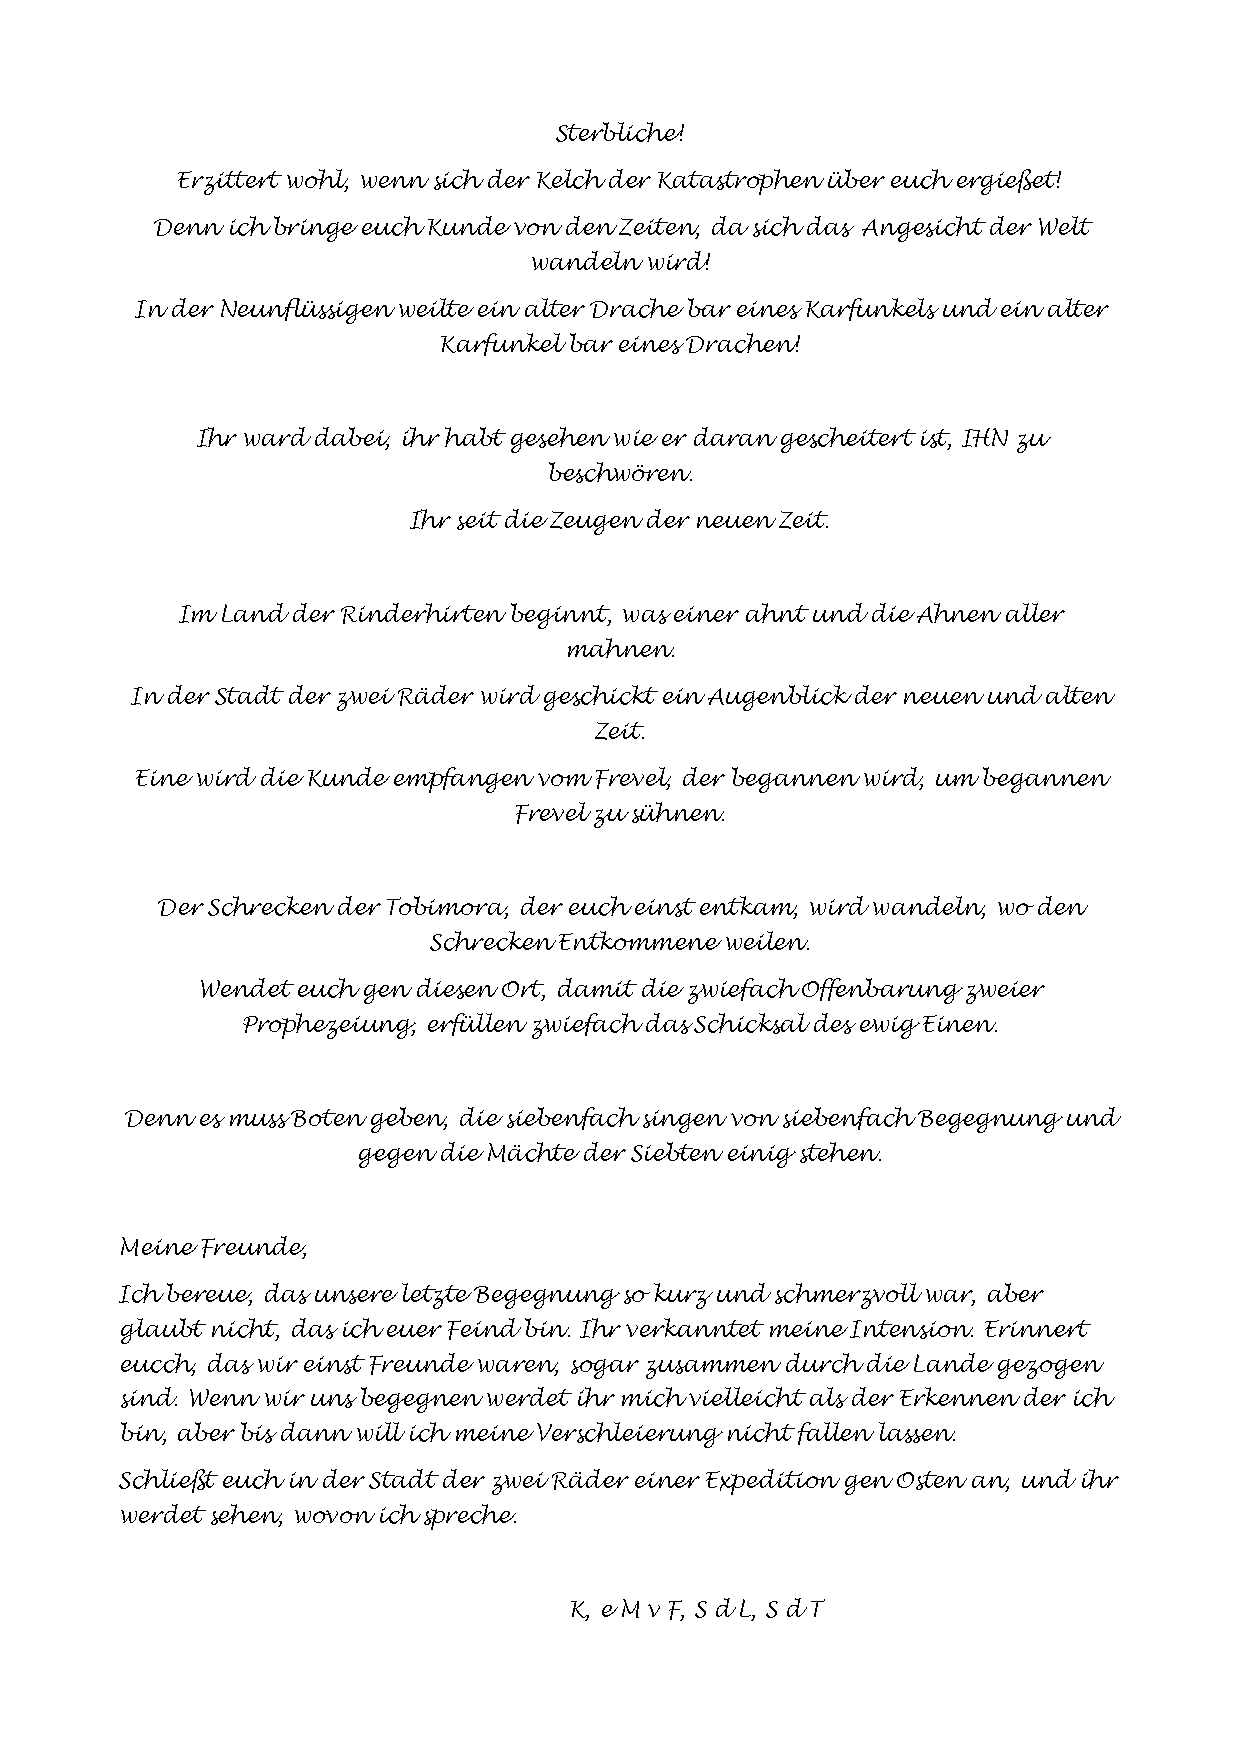
\includepdf[scale=0.9,pages=-]{handouts/part_1/aoe_brief_markhalm.pdf}

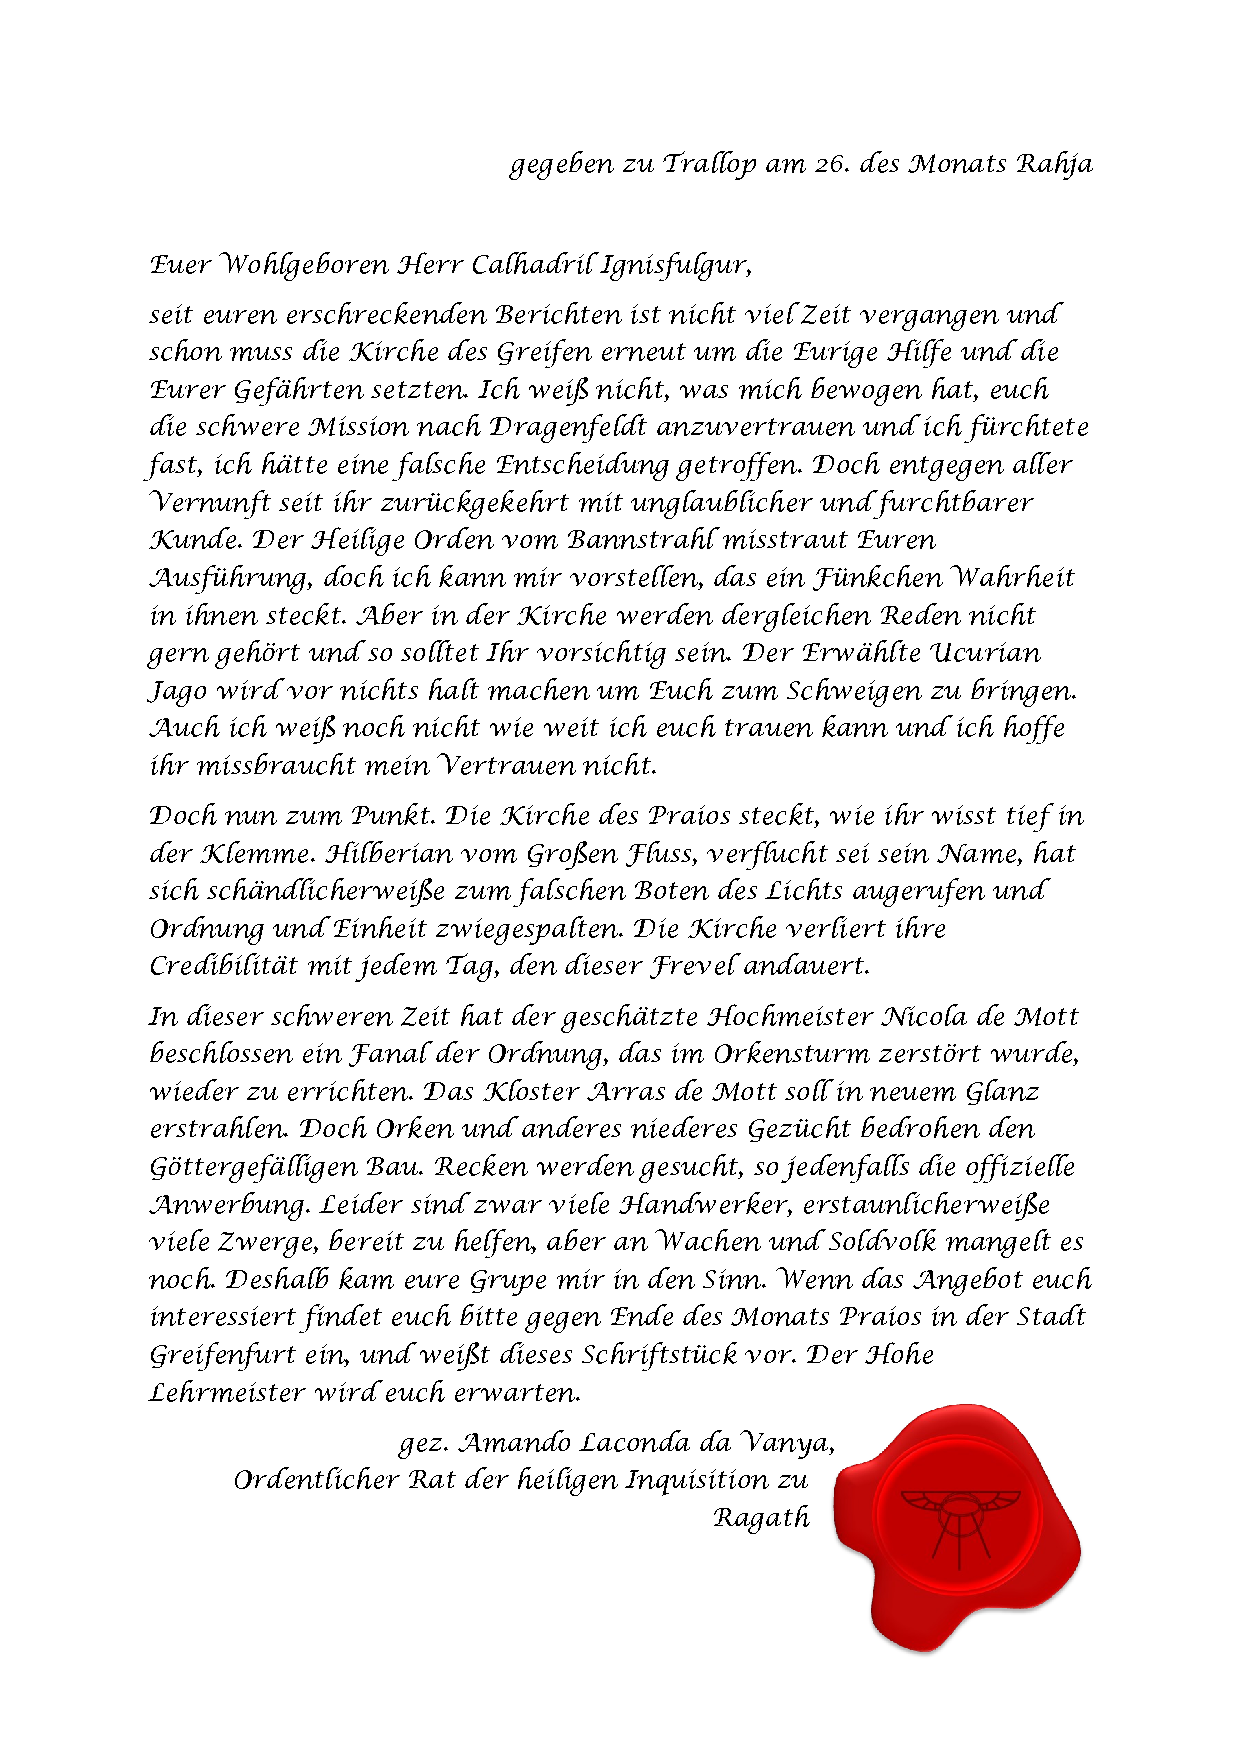
\includepdf[scale=0.9,pages=-]{handouts/part_1/gm_brief_temyr.pdf}


\includepdf[scale=0.9,pages=-]{handouts/part_1/ug_waldemars_brief_Thoran.pdf}

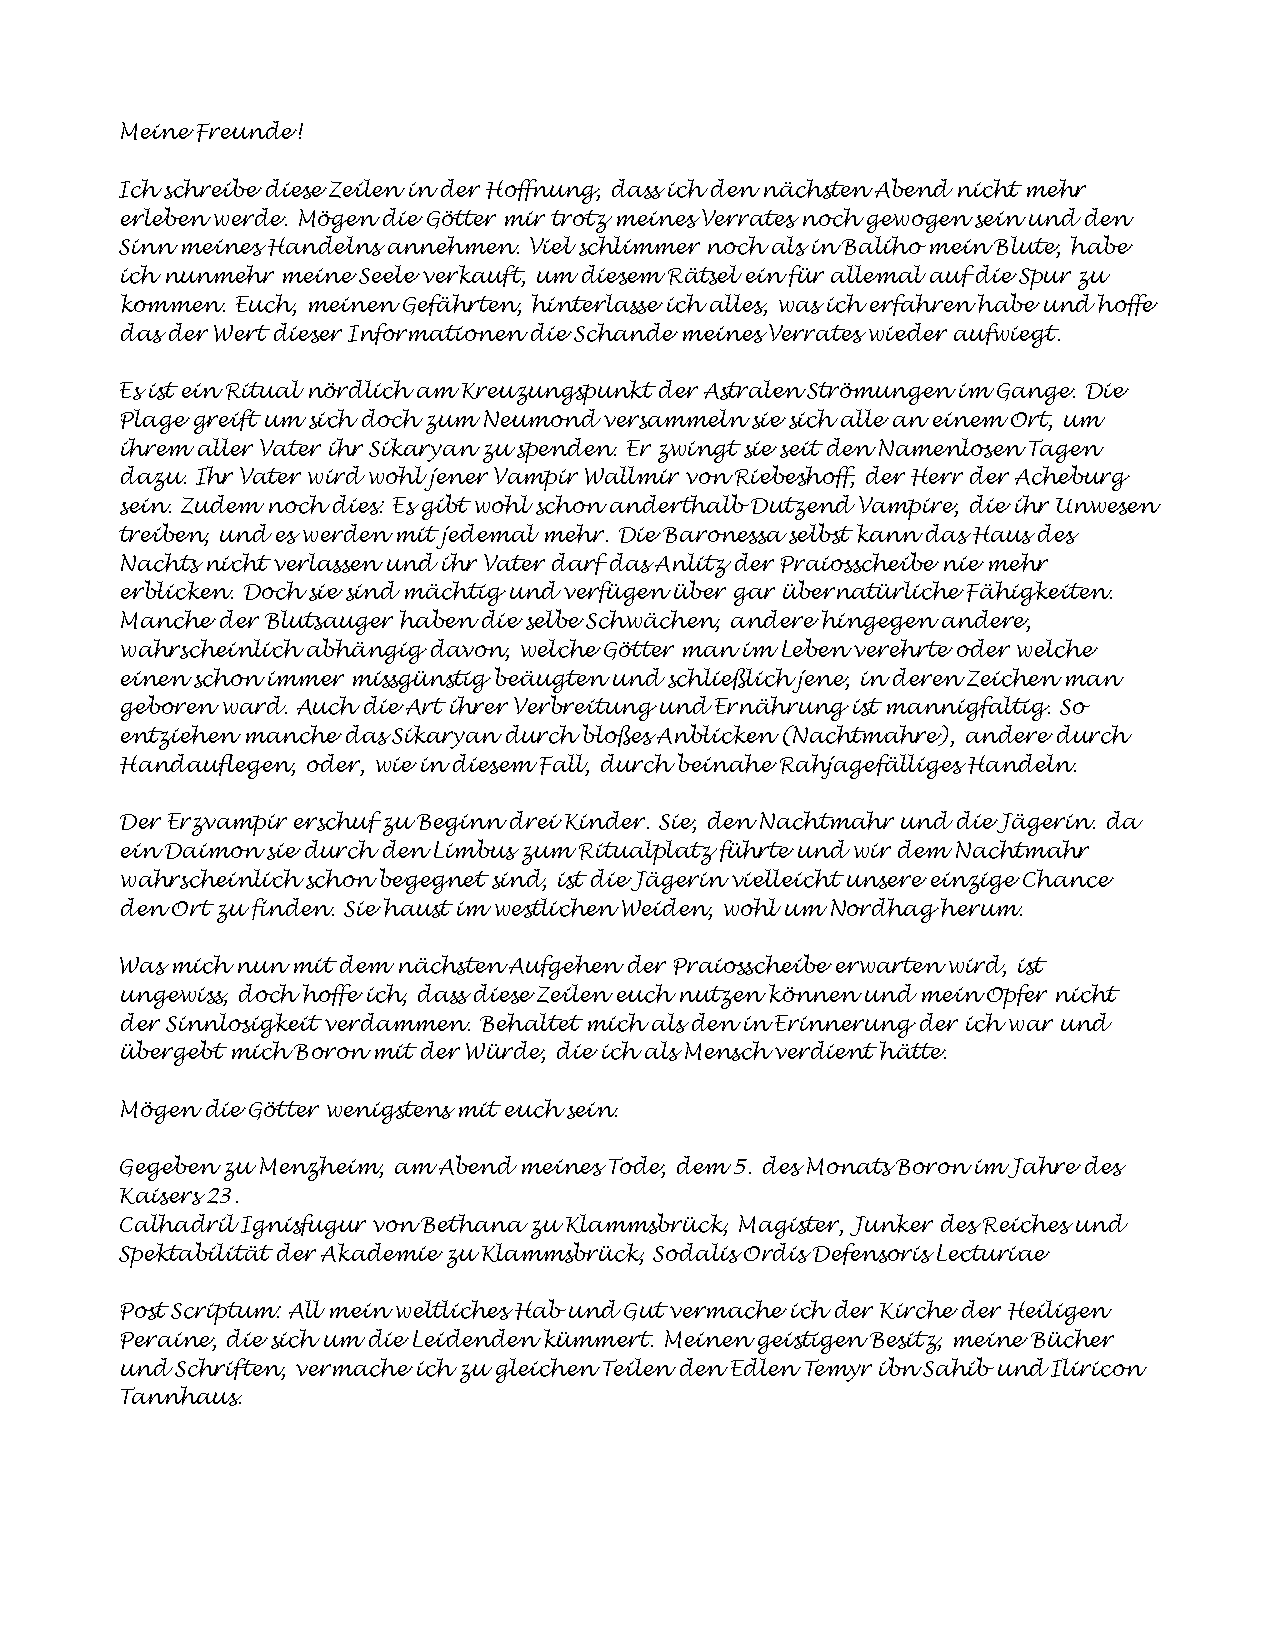
\includepdf[scale=0.9,pages=-]{handouts/part_1/ug_abschied_calhadril.pdf}

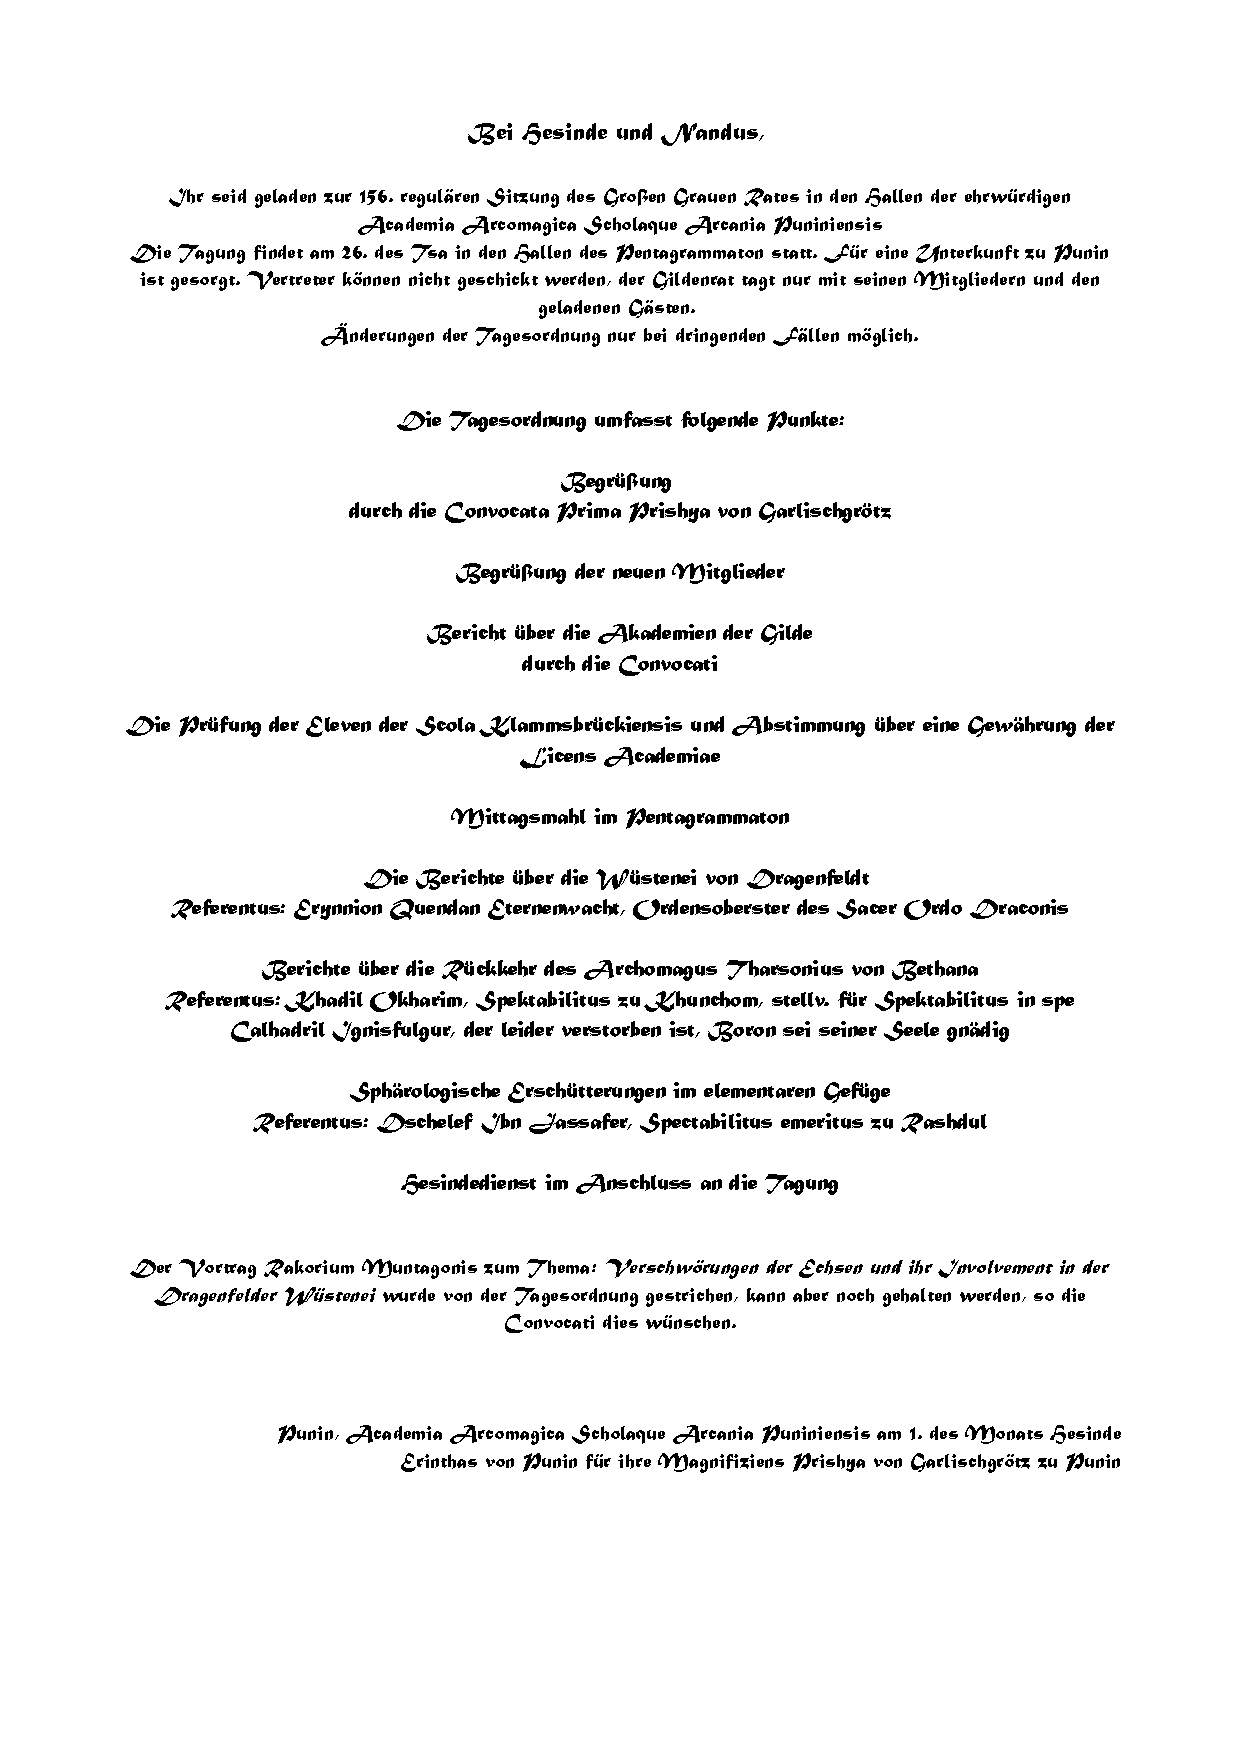
\includepdf[scale=0.9,pages=-]{handouts/part_1/einladung_gildenconvent_ggg.pdf}

\part{Meister der Dämonen}
\chapter{Euch zum Geleit}
Lang, lang ist es nun her dass die Gezeichneten gefallen sind. Während ich die Tagebücher der Rückkehr der Finsternis noch in Darmstadt zusammen gesammelt habe, ist es nun fast 10 Jahre her dass wir unsere Runde beendet haben. Naja, nicht ganz, aber 10 klingt dramatischer als 9.

Die Bücher der Borbaradkampagne sind inzwischen in Philips Besitz über gegangen, und ich glaube ich habe seit mehr als 5 Jahren kein DSA mehr gespielt. Es ist schwierig Leuten zu vermitteln dass sie erstmal 3 Bücher auswendig lernen müssen um dann vlt ab und an (wenn man es überhaupt organisiert bekommt) einen Spielabend besuchen zu dürfen :). Aber selbst in Kanada bin ich dem Hobbz treu geblieben und habe, zusammen mit Freunden aus aller Welt, über einige Jahre eine erfolgreiche Kampagne an einem der größten KI Forschungsinstitute Nordamerikas organisiert.

Diese Projekt habe ich wieder aufgegriffen als ich angefangen habe zu überlegen, was ich zu Philips Hochzeit vorbereiten könnte. Mein alter Laptop aus Darmstadt hatte den Zwölfen sei Dank noch eine komplette Sicherheitskopie des alten Forums! Und so ist dieses zweite Buch vor allem und natürlich euch, aber auch unseren Partnern und Partnerinnen gewidmet. Amor vincit Omnia!

\chapter{Bericht über die dreuenden Schatten}


Mein liebster Waldemar,

Es war eine sonderbare Zeit, nach der Verkörperung, aber vor dem Angriff der dämonischen Horden.
Nur wenige wussten um das was uns bevorstehen würde, und ich gestehe, selbst ich war mir nicht sicher ob alles wahr was, was sie mir erzählten.
Nachdem die Rückkehr des Dämonenmeisters vor allem im Weidenschen stattfand, führten diese Ereignisse unsere Freunde in weit entfernte Lande.
Eine zeit lang reisten sie alleine durch die Gegend, und versuchten Verbündete gegen die drohende Gefahr zu finden.

Dein alter Lehrmeister,\par
Spektabilitus Emeritus Iliricon Tannhaus, Chronist des Sacer Ordo Draconis



\chapter{Pforten des Grauens}

\section{Geleitwort}

Die Kommentare werden nun wohl noch schwieriger werden, nachdem ich weitere 5 Jahre habe verstreichen lassen. Trotzdem, Pforten des Grauens hat mir persönlich wahrscheinlich fast am meisten Freude bereitet. Wobei das vielleicht etwas zu viel über meinen Hang zum Sadismus aussagt? Mir ist noch sehr deutlich in Erinnerung was für eine Folter dieses Abenteuer für die Helden war, und ich habe Stunden damit verbracht, mir die bescheuertesten Kreaturen auszudenken.

Reine Wildnisabentuere sind oft schwierig besonders interaktiv zu gestalten, weil die Wildnis einfach nicht viele Müglichkeiten für gute Spielentscheidungen liefert. Ich hoffe, es ist euch trotzdem eher als spannende Geschichte und weniger als kitschiger Horrorvorleseroman in Erinnerung geblieben. Nachdem ich vor kurzem einige Tage in Sngapore verbracht habe, habe ich inzwischen deutlich mehr Mitleid mit armen Abenteurern, die sich durch schwüle Hitze schlagen müssen.

Die mir am besten in Erinnerung gebliebenen Szenen sind:
\begin{itemize}
\item Jagdgraß, eine wirklich gruselige Vorstellung für einen Campingurlaub
\item keine Szene an sich, aber eine unserer längsten Spielabende an Victors Geburtstag bei ihm zu Hause, bei dem wir wirklich alle fast eingepennt sind
\item Victors nächster Charaktertod, wirklich schnell nach dem vorherigen
\end{itemize}


\begin{flushright}
Claas Völcker, Toronto, den 25.05.2025
\end{flushright}


\section{Die Tagebücher}

\subsection{Maraskan aus ``Blutrosen und Marasken''}
Informationen aus den Büchern des Hesindetempels:

Die maraskanische Hauptinsel hat eine Länge von rund 650 Meilen und mißt an der breitesten Stelle etwa 250 Meilen. Dem Südzipfel Maraskans sind (von Nord nach Süd) die Inseln Jandraskan, Etlaskan und Jilaskan vorgelagert, der Südostküste (ebenfalls von Nord nach Süd) die Inseln Buli, Saijana und Andalkan sowie dort etliche namenlose Eilande mit häufig wechselnden Küsten. Direkt unter der Südspitze Maraskans, nur wenige Meilen von Sinoda entfernt, liegt die ``Affeninsel'' Beskan.

Abgesehen von einem schmalen Küstenstreifen von 10 bis 20 Meilen Breite ist die Insel bergig bis gebirgig und mit dichten Urwäldern bedeckt. Wie ein steinernes Rückgrat zieht sich die Maraskankette von Norden nach Süden. Eine schmale Senke trennt sie vom zerklüfteten Amdeggynmassiv. Die höchsten Berge sind der Amran Gerbald (6.500 Schritt) im Norden der Insel und der Amran Thjemen (6.300), der ziemlich genau im Schwerpunkt des Dreiecks Jergan-Boran-Tuzak liegt. Dagegen wirken die höchsten Erhebungen des Amgeggyns -- Amran Thurak (3.400 Schritt) und Amran Thjalgyn (3.200) -- fast bescheiden. Die Insel besitzt vier größere Flüsse, die in etwa den vier Himmelsrichtungen folgen, und zwar den Hira im Norden, die Mendrina im Osten, den Roab im Süden und die Obogyn im Westen. Mehrere kleinere Flüsse münden in sie. Die Küstenlinie weist zahlreiche Buchten auf, die schon immer beliebte Piratenverstecke waren. Auch nach achthundert
Jahren Besiedlungen sind große Teile des maraskanischen Binnenlandes unbekannt.

Das Küstenklima ist angenehm, auch wenn es oft von Festlandsbewohnern gleicher Höhe als zu heiß eingeschätzt wird. Im Landesinnern hingegen herrscht ganzjährig eine unerträgliche, schwül-drükkende Hitze vor, die erst in den größten Höhen der Maraskankette, deren höchste Gipfel auch im Winter nur selten von Schnee bedeckt sind, gemäßigten Temperaturen Platz macht. Die Hauptregenzeit ist zwar im Phexmond, verschiebt sich jedoch gelegentlich um mehrere Wochen. Schwere Regenstürme überziehen dann die ganze Insel und lassen die Flüsse über die Ufer treten. Eine zweite, kleinere Regenzeit (von den Einheimischen nicht als solche bezeichnet) tritt im Frühherbst ein. Generell ist die Osthälfte der Insel wesentlich feuchter als
die Westhälfte.

Zu den vielen Eigenheiten der maraskanischen Pflanzenwelt gehört eine starke Rottönung des Blattwerks während des kurzen Winters, so daß das Rot der Wälder, unterbrochen vom Gelb der verdorrten Felder und Lichtungen, dem Ocker und Schwarz der Berge aus der Luft an den Rücken einer Maraske erinnert. Typisch für die Flora der Insel ist eine Neigung zum Riesenwuchs, was sich nicht nur in Baumriesen ausdrückt, sondern etwa auch in Farnen mit über drei Schritt hohen Wedeln.

Der maraskanische Dschungel gilt als einer der gefährlichsten Wälder ganz Aventuriens. Nicht wegen Großraubtieren, von den es nur wenige Arten gibt, sondern wegen seiner Schlangen, seines schier unendlichen Artenreichtums an kleinen und kleinsten, oft giftigen Lebewesen und nicht minder bedrohlichen giftigen und fleischfressenden Pflanzen, von denen sogar einige Arten -- wie etwa Jagd- und Fallgras -- selbstbeweglich sind. Das nachfolgende Zitat des Magisters Majian da Meran ist keineswegs eine Übertreibung: ``Die maraskanischen Wälder stelle man sich besten wie ein Land vor, um dessen Besitz viertausend Könige gleichzeitig erbittert kämpfen. Jeder von ihnen hat mächtige Heerscharen aufgeboten. Menschen gelten nicht als kriegsführende Partei. Sie sind nur für die Provianteure und Marketenderinnen von Interesse.''

Die einheimische Tierwelt -- wir nehmen hier die Tierarten aus, die seit der Besiedlung eingeführt wurden, wie etwa Phraischaf oder Rind -- kennt nur wenige Großtiere, erwähnt seien Perldrache, Maran, Parder, Maraskantarantel, der waschbärgroße Baumwürger, der Harnischgürtler oder das mittlerweile äußerst seltene maraskanische Wollnashorn. Eine größere Vielfalt zeigen kleinere Tiere wie Mungo, Stinkfrettchen, Baumschleimer, Biberratte, das giftige Stachelschwein und verschiedene Kleinaffenarten. Unter Berücksichtigung der Unerforschtheit großer Teile der Insel sind diese Aussagen mit einem gewissen Vorbehalt versehen: Es gilt als nicht sehr wahrscheinlich, daß der Tuzakwurm der einzige Vertreter seiner Art auf der Insel war, auch wenn seither kein ähnliches Tier mehr gesichtet wurde.

Maraskan ist reich an Bodenschätzen: Das Gestein der Maraskankette enthält Kupfer, Quecksilber, Zinn, Blei und Eisen, letzteres vor allem im Südwesten in gehaltvollem Erz, doch auch Edelmetalle sind in geringerem Maße vorhanden, hinzu kommen Alabaster und Graphit; berühmt ist die Insel wegen der einzigen zugänglichen Enduriummine Aventuriens. Doch auch die Wälder Maraskans sind eine Schatztruhe für Heilkundige, Gewürzsucher, Giftmischer und Alchimisten. Traditionelle Anbauprodukte der Insel sind Zuckerrohr, Reis, Pfeifenkraut, Tee, Shatak, Obst und Mandeln. Die bekanntesten Ausführgüter waren bisher Edelhölzer, die als Roabwolltuch bekannte Phraischafwolle, Gewürze wie Paprika, Pfeffer oder Ingrim, Heilpflanzen, Erze und Tuzaker Stahl.

Das maraskanische Volk zählt nach unterschiedlichen, stark divergierenden Schätzungen 80.000 bis 150.000 Köpfe. Bis vor rund dreißig Jahren galt: Ein Sechstel aller Maraskaner lebt in den vier Städten Jergan, Boran, Sinoda und Tuzak, ein weiteres Fünftel in etwa vierzig Ansiedlungen, manchmal so groß wie Kleinstädte, in ihrer nächsten Umgebung, der Rest in zahllosen kleinen Dörfern, Weilern, Gehöften und auf Plantagen, von denen die wenigsten mehr als fünfzig Meilen weit im Landesinneren lagen.


\subsection{Die Anreise nach Firnen}
\paragraph{20. Ingerimm 1018 BF}
Heute kam Arngrimm mit einer Boronia vorbei. Sie überbrachte uns den Aufruf uns in Punin vor dem hl. Raben einzufinden. Ich denke wir werden gleich morgen aufbrechen.

\paragraph{22. Rahja 1018 BF}
Sind vorhin in Punin angekommen. Ein ziemlich großes Gebäude dieser Borontempel. Die Boronkirche (sowohl Punier- als auch Al'anfaner-Ritus) sendet uns aus, illegal auf Maraskan Nachforschungen über eine Endurium- Lieferung anzustellen, die verschwunden ist (nicht einmal ein Zeichen auf dem Schwarzmarkt, deshalb wahrscheinlich nicht die Rebellen.) Zur Überfahrt wird uns in Kunchom eine Zedrakke erwarten.

\paragraph{1. Prajos 1019 BF}
Die Namenlosen Tage haben wir in einem Dorf, eine Stunde vor Zhammorah, verbracht. Im Anschluss habe ich mich an den Rand der uralten Ruinen begeben, sehr zur Freude Zulhamids (Zulhamid iben Zahier = das almadiene Auge), welcher mir eine eindrucksvolle Stadtbeschreibung gab. Außerdem offenbarte er mir den mächtigen astralen Nodix, dessen Kraftlinien seltsam zerrissen und zerfranst schienen. Die Stadt strahlt etwas dunkles aus, aber auch die Verlockung uralter Geheimnisse und Macht. Wer kann sagen, was man in Zhammorah alles zu finden vermag, und welche Schrecken vergangener Beschwörungen noch immer lauern, bereit jeder Zeit wieder zu erscheinen. Sehr bedeutend schien auch ein gewisser Bastrabun zu sein (ich glaube Erbauer der Stadt\footnote{Was für eine gescheiterte Geschichtswissen-Probe spricht.}). Zhulhamid erwähnte ihn häufig und sprach auch von den Fünf Obelisken von Bastrabuns Bann. Die Stadt zu betreten wagte ich nicht

\paragraph{4. Praios 1019 BF}
Haben Kunchom erreicht. Habe mit Kadil O'Karim gespeist und einen fünmal nutzbaren Abvenumstein erhalten -> Gegenleistung= ein kleiner Gefallen der noch aussteht.
Ich habe mir auch die astralen Strömungen in Kunchom angesehen, der Nodix-Astralis scheint gestört, und auch Temyr meinte etwas von einer spürbaren "Schändung der Elemente"
Habe außerdem in Reiseberichten von zwei Hesindegeweihten einiges über Maraskan geslesen, hauptsächlich zu ihrer Kultur. Wichtige Erkenntnis: Irgendwie sind die Maraskaner untereinander über ein paar Ecken alle verwandt. Dies führt zu einem leichten Paradoxon bei Familienfehden zwischen zwei Familien (oder wäre es nicht eigentlich dann innerhalb einer Familie / der Familie: "Maraskan"?)

\paragraph{5. Prajos 1019 BF}
Sind heute ausgelaufen. Haben die Passierscheinkontrolle gut überstanden. Hängen jetzt kurz vor Maraskan in der "Flaute vor dem Sturm"

\subsection{Der Sturm nach Ragnos}

\paragraph{5. Praios}
Ein Windhauch streicht über meine Wange, als ich Richtung Maraskan schaue, welches nicht mehr weit entfernt sein sollte. In diesem Moment werde ich der tief schwarzen Wolken am Horizont gewahr, wie auch der Rest der Mannschaft an Bord. Es bricht Hektik aus, die Seeleute beginnen Ladung zu vertäuen und die Segel einzuholen, auch ich beginne unsere Ausrüstung in Bündel zu schnüren und zu sichern. Der Wind nimmt zu und ein Schaukeln ergreift das Schiff welches uns hin und her wirft, als auch die Wellen sich zu echten Wänden auftürmen. Ich sehe noch wie eine gewaltige Welle den Steuermann erfasst und in den Fluten verschwinden, Boron sei ihm gnädig. Firnen hangelt sich Richtung Ruder und versucht einen Kurs zu halten, auch wenn ich nicht weiß wir er diesen bestimmt. 

Plötzlich kehrt Ruhe ein und ein kurze Pause wird uns gewährt, während das Auge das Sturms über uns zieht. Toran heilt und versorgt die schwer verletzten Matrosen wo er nur kann doch bei einigen reichen auch die Segen der Perain nicht aus. Der Kapitän geht seiner grausamen Pflicht nach und überreicht die nicht mehr zu rettenden Boron und der ewigen See. Doch es bleibt kaum Zeit die Toten zu betrauern und um ihre ewige Ruhe zu bitten. 

Die übrigen Verletzten werden unter Deck vertäut und von Toran in einen heilenden Schlaf gelegt. Firnen hält das Ruder und bindet sich zusätzlich an der Reling fest um nicht wie der Steuermann über Bord zu gehen. Da bricht auch schon mit einem Schlag die schwarze wirbelnde Wand über uns herein und zerfetzt den Hauptmast, welcher nun droht das Schiff in die See zu ziehen. Zum Glück schaffen wir es noch die Seile zu kappen. Ein Ruck geht durch das Schiff und Schlag aus dem Bug lässt mich darauf schließen das sich die Ladung gelöst hat und dabei die Wand zerschlagen hat. 

Als kurz darauf die letzten beiden Masten abbrechen und dem Sturm zum Opfer fallen, greifen wir uns unsere wichtigsten Habseligkeiten und Ausrüstung um anschließend über Bord zu springen. Wasser ist überall, in meinen Augen, meinen Mund, um mir herum und wir schwimmen immer weiter weiter bis alles schwarz wird \dots

\paragraph{6. Praios}
Es ist hell mitten am Tag. Ich denke es der 6 doch ich bin mir nicht mehr sicher.
Als ich mich aufsetzt wird mir kurz schwarz vor Augen, dann sehe ich 300 Fuß entfernt eine grüne Wand, da wird mir bewusst, dass wir es geschafft haben, wir sind auf Maraskan, der grünen Hölle. Als ich meine Freunde gefunden habe und einige verbliebene der Schiffsbesatzung, bauen wir ein Lager am Rande des Dschungels auf. Toran vollbringt dort ein wahres Wunder, er ruft einen Krug welcher nicht auszutrinken ist und wenn ihr mir es nicht glaubt mögt, ich habe es selber versucht. Als wir 3 Stunden später ein neues Lager aufbauen in der nähe eines Flusses, verschwindet Toran im Dschungel, er sagte irgendwas von einer Pflanze und der Harmonie mit der Natur.

Am Abend legen wir uns erschöpft schlafen, leider scheint aber auch die Wache der Schlaf überkommen zu haben, da ich unsanft von einem Schlag in den Rücken geweckt werde und ich in ein wenig schmeichelhaftes Gesicht eines Rebellen aufsehe, wie ich vermutete. Nach einer kurzen Rangelei werden wir in den Dschungel geführt, ich verstehe kein Wort aber das haben diese verdammten in Maraskan so an sich. Nach einem längeren Gespräch mit dem Anführer erhalten wir von diesem Ausrüstung und Wasser und einen Führer, da er unseren Auftrag anscheinend für sinnvoll hält ich weiß es nicht.

\paragraph{7. Praios}
Nach einem wenig geruhsamen Schlaf bei den Gefangen, brechen wir auf mit unserem Führer in den Dschungel. Nachdem wir eine Marschordnung gefunden haben, finden wir uns schon bald tief im tiefem Grün wieder. Nach kleineren Hindernissen und einigen befremdlichen Tieren lässt uns unserer Führer eine Wasserquelle suchen, um darin etwas Übung zu haben bevor er uns am nächsten Tag verlassen wird. 

Nach kurzer Zeit finde ich mit meinen Kenntnissen der Natur einen Tümpel. Als Firnen jedoch Wasser schöpfen will greift ihn plötzlich ein Alligator an und in diesem Moment fallen mir weitere seltsame Schatten im Wasser auf und einige weiter Alligatoren kommen aus dem Tümpel. Nach einigen Ignifaxius Zaubern und einigen wohl platzierten Schüssen, sowie kräftigen Schwertstreichen, ziehen sich die Alligatoren zurück und lassen nur einen Toten Artgenossen zurück, welchen ich mit etwas Mühe frisches Fleisch entnehmen kann. 

Nachdem wir unsere Wasservorräte aufgefüllt und gereinigt haben, machen wir uns wieder auf in die alles verschlingende grüne Hölle, bei allen zwölften wie ich diese Insel jetzt schon hasse.

\subsection{Die ersten Tage auf Maraskan nach Temyr}

\paragraph{Maraskanexpedition 3. Tag}
Nachdem wir die geschuppten gûl zurück in ihr brackiges Wasser gescheucht hatten, füllten wir unsere Taschen mit zähem, sehnigem Fleisch, derweil Thoran sich der Wunden unseres halbelfischen Freundes annahm. Ich fürchte, in diesem maldrûn Dschungel wird die Versorgung von Kranken ein schwieriges Unterfangen werden, zumal die Moskitos und die drückende Hitze -- gegen welche die khunchomer Wärme eine schmeichelnde Brise ist -- auch uns Gesunden arg zusetzt. 

Wir setzten den Gewaltmarsch fort, nicht ohne ein ungutes Gefühl meinerseits, welches ich jedoch als unbedenkliche Nichtigkeit abtat. Das Letzte woran ich mich deutlich erinnere sind Koliken, Fieberschütteln und Halluzinationen, zu denen sich die Beschwerden erwuchsen… Dieses Land haben selbst die seleyah -- der große Bastrabun möge meine Worte verzeihen -- nicht verdient, das einen Mann derart vertrocknen und verfaulen lässt. (Die nächsten Zeilen sind angefüllt mit wüsten Flüchen und Verwünschungen, die einen Al`Anfaner Kopfschlächter zum Erbleichen bringen könnten, glücklicherweise aber auf Urtulamidya verfasst sind.)

\paragraph{4. Tag}
Wie dem auch sei, müssen meine Gefährten um mein Wohl während der Umnachtung besorgt gewesen sein, denn den nächsten Morgen erwachte ich mit neu erwachsenen Kräften und ohne Anzeichen meines vorabendlichen Kollapses. Dies, so wird sich zeigen, sollte uns zum Vorteil in einer späteren Auseinandersetzung gereichen. Zuvor sahen wir uns jedoch einem natürlichen Hindernis ausgesetzt: Ein Gehölz aus scharfen Dornen und kräftigen Ranken erstreckte sich zu allen Seiten unseres Pfades, dem wir seit den frühen Morgenstunden gefolgt waren. Nach Erwägung der uns gegebenen Wegbeschreibung und dem Rat der Sterne entschlossen wir uns für ein Umgehen des Dickichts, was gerne den halben Praioslauf in Anspruch nahm. 

Mit dem Erreichen des ausgewiesenen Sumpfes setzte auch der beständige Regenguss wieder ein, der auf Maraskan wegen der besonderen klimatischen Verhältnisse alltäglich herabfährt. Vom nassen Element umgeben fuhren wir in unserem Marsch fort, bis auf einmal die dunstverhangene Luft von einer Vielzahl klebriger Fäden zerteilt wurde und Rezzanjins Beine umschlungen. Wir duckten uns sofort hinter die Pfahlwurzeln naher Bäume und versuchten, des Aggressors gewahr zu werden, doch durch den feinen Nebel war nichts auszumachen. 

Bedächtig tasteten wir uns in die Richtung des Schusses, bis Arngrimm wortlos auf eine Baumruine vor uns deutete. Dort, von den knorrigen Ästen hängend, sahen wir zwei weiße, fahläugige und für meinen Geschmack deutlich zu große Spinnen. Der Weidener löste seinen Bidenhänder in der Scheide und stürmte auf die Monstrositäten zu, während ich eines günstig hängenden Astes über ihnen ersichtig wurde. Mit eines einfachen Motoricus` Hilfe verstärkte ich seinen natürlichen Wunsch, Sumus` Griff nachzugeben und ließ ihn auf die Spinnen fallen. Eine wurde durch die Wucht des Treffers und des eigenen Aufschlages getötet, die andere fällte Arngrimm mit einem kühnen Schwertstreich. 

Nach diesem denkwürdigen Zwischenfall suchten wir einen Rastplatz für die Nacht, einen solchen erspähte Ragnos mit geübtem Auge. Wie betäubt fielen wir in tiefen, in meinem Fall traumlosen Schlaf.

\paragraph{5. Tag}
Der nächste Morgen graute unter wenig guten Voraussetzungen. Als wir erwachten, fanden wir Thoran in einem fürchterlichen Zustand vor: Aus seinen Armen und Beinen brachen aus schwarz geränderten Wunden Büschel von Gras, so als wollte eine Pflanze aus seinem Innern erwachsen. ``Jagdgras``'', meinte Rezzanjin, ``wir werden es ausbrennen müssen.``'' Nach seiner Anleitung verfuhren wir und entfernten das Unkraut aus Thorans Körper -- der Anblick war nicht erbaulich. Geradezu erfreulich stellte sich hingegen der Gesundheitszustand meines geschätzten Collegus Firnen heraus, der über Nacht komplett genesen zu sein schien. 

Wenig gestärkt brachen wir zu einem weiteren Teil unserer Durchquerung auf, der bis auf einen Moment vollkommener Stille im Wald dankbarerweise ereignislos verlief, bis wir an die ersten Ausläufer des maraskanischen Primärwaldes gelangten. Etwa um die Mittagsstunde gelangten wir nämlich auf eine Lichtung, welche einen grausamen Fund bereithielt: Auf blutgefärbtem Waldboden, das Herz aus dem geöffneten Brustkorb gerissen, lag dort die Leiche eines Echsenmannes. Seine Kleider waren überreich mit Musterungen und Applikationen versehen und in einer seiner Taschen fanden wir einige Edelsteine, weshalb Firnen und ich auf ein Mitglied der Kristallomantenkaste schlossen. 

Angsterfüllt schlugen wir einen Weg gen Osten ein, so wie es uns einer der Rebellen geraten hatte. Hier wucherten allerorts große Pilze mit schwarzgefleckten Fächern aus dem Boden, manche davon einen Schritt hoch. Zu gerne hätte ich eines dieser Gewächse näher untersucht, doch eine Probe wäre unnötiger Ballast auf unserem kräftezehrenden Marsch gewesen. 

Einige Zeit später hallten unvermittelt durchdringende Schreie durch den Baumstand, und als wir unsere Blicke zum Himmel wandten, sahen wir dort einen Schwarm großer Vögel mit scharfen Krummschnäbeln, die über einer vor uns liegenden Lichtung ihre Kreise zogen. Kaum hatte Rezzanjin seinen Fuß auf diese gesetzt, so stürzten sich die Flugbestien auf ihn und hackten mit ihren Krallen nach ihm. Wir entschlossen uns einstimmig, um die Lichtung herumzugehen, eine Entscheidung, die wir im Nachhinein noch bereuen sollten. Das Gebüsch, welches wir der fliegenden Gefahr vorzogen, war nämlich von weitaus gefährlicheren Übeln bewohnt. 

Abermals wurde Rezzanjin, welcher vorne mit Arngrimm lief, angefallen, doch mit welchen Folgen! Urplötzlich schoss, nur als weißer Schemen erkennbar, eine armdicke Schlange aus einem Strauch in der Nähe und verbiss sich in seine unbedeckte Haut. Noch im Sturz durchstieß Rezzanjin das Ungetüm und nagelte es in die weiche Erde, als Arngrimm vorsprang und der zweiten lauernden Viper glatt weg den Kopf abhieb. Thoran eilte dem Getroffenen zu Hilfe, der, all gesunder Lebensfarbe beraubt und am Leib zitternd, keuchend auf dem Boden lag. Verzweifelt kniete der Geweihte neben ihm und musste ansehen, wie die Kraft aus dem Körper unseres Gefährten rann. Doch die Göttin der Felder hatte Erbarmen mit Rezzanjin, und so sollte er weiterhin auf unseren Pfaden wandeln. Doch der Erfolg der Behandlung blieb für uns zunächst ungewiss…

\subsection{Die Hochzeit nach }

Wieder sind wir einer Bestie der grünen Hölle entkommen. Dank Thoran kann Rezzanjin sich wieder bewegen und so brechen wir wieder auf in die Richtung des Herzen dieser verderbten Insel Maraskan und ich will nicht wiesen was uns noch an tödlichen Gefahren erwartet. Ich sehe nur grün, grün und noch mehr grün und man weiß nie was einen nach ein paar Metern erwartet. 
Temyr sagt er höre menschliche Stimmen aus nördlicher Richtung, ich höre nur die Geräusche des Dschungels. Woher weiß er eigentlich bei diesem dämmrigen Grün aus welcher Richtung die Stimmen kommen?

Nach Stunden, so kommt es mir vor, erreichen wir einen Pfad, es ist erste Zeichen von Zivilisation auf diesem götterverlassenen Eiland. Es entbrennt eine Diskussion in welche Richtung wir gehen sollen, schlussendlich entscheiden wir uns Richtung Süden zu begeben. 

Endlich verlassen wir den Dschungel und ich wünschte mir müssten ihn nicht nochmal betreten, aber die Ohren der Götter sind taub. Der Pfad führt über einen Damm durch eine Sumpflandschaft und Ragnos schießt einen fremdländischen Vögel, der laut Rezzanjin eine Spezialität ist, aber bei manchen Rebellen als heilig gilt. Weiter dem Damm runter finden wir eine zwei Tage alte Lagerstätte, dort bereitet Ragnos den Vogel vor und wir braten den Vogel über den Flammen der Zauberstäbe. Wir lassen den allabendlichen Regen über uns ergehen, der anscheinend abnimmt. 

Wir raffen uns nochmal auf, um noch etwas weg zurückzulegen. Hinter einem Hügel erblicken wir einen Bauernhof. Es öffnet uns ein kleines Mädchen, das meint:``Ihr stinkt!`` Die Hausherrin lässt uns herein, davor müssen wir alle baden, wobei Firnen als Letzter dran ist und zweimal muss, da er in irgendwelchen Käfern geschlafen hat. Während wir ins Haus gehen, muss Firnen die Nacht in der Scheune verbringen. Es gibt Reis zu essen, die Gastfreundschaft und Küche dieses Landes ist exquisit. 

In dieser Nacht habe ich einen Traum, an den letzten kann ich mich nur noch schwach erinnern, es kommt mir vor, als wäre es in einem anderen Leben geschehen. Ich wache frühmorgens auf und warte bis die anderen aufstehen. Die alte Frau erklärt uns den weg nach Alrurdan und rät uns im Rur \& Gror-Tempel nachzufragen, wenn wir den Haran suchen.

Am selben Nachmittag brechen wir nach Alrurdan auf. Dort erfahren wir im Tempel, dass wir alle steckbrieflich gesucht werden. Firnen wir im Fort vom Kommandanten erkannt und kann gerade so in den Tempel fliehen. Eine Nacht verbringen wir in Alrurdan. Ein Priester will uns zum Haran führen. Um nicht erkannt zu werden, färben wir uns mit einen Kraut die Haare.

Schon wieder betreten den Dschungel, aber diesmal den inneren tödlicheren Teil. Ich verstehe nicht, warum das Mittelreich so viele Ressourcen für diese Insel verschwendet, außerdem sind mir auf Maraskan mittlerweile die Rebellen deutlich sympathischer als diese von der KGIA gesteuerten Gardisten.

Unser Pfad kreuzt sich einmal mit dem Weg einer Patrouille, die aber zu unserem Glück ihre Steckbriefe vergessen hat. Später stoßen wir auf einen Kampfplatz, wo der Diskus von Boran gegen den Dajin gekämpft hat. Abend kommen wir zu einem Dorf, indem gerade eine Hochzeit gefeiert wird. Rezzanjin und ich lassen uns die Haare noch einmal färben. Während die anderen feiern, bleibe ich nüchtern und ausgerechnet mir passiert es, dass die Braut sich an mich schmiegt und der Bräutigam mich schlagt. Ich beherrsche mich und schlage nicht zurück, weil es anscheinend ein maraskanischer Hochzeitbrauch ist. Mitten in die Feier platzt der Weibel der Patrouille mit elf Drachengardisten. Er hält die Feier für rebellische Umtriebe und will alle verhaften. Nach dem wir den Weibel, seine beiden Korporale und drei weitere Soldaten getötet haben, flieht der Rest. Derweil sinke ich halbtot und fast ohnmächtig zu Boden.

\subsection{Rebellen nach Rezzanjin}

\paragraph{Mitte Praios im Lager des Haraniadad}
Nachdem wir den Hauptmann und die Weibel niedergerungen hatten, flohen die restlichen mittelreichischen Feiglinge. Doch wir und die Dorfbewohner waren nicht ohne Wunden davongekommen. Zwei Tote gab es auf Seiten des Dorfes zu beklagen. Zu ihnen zählte unserer Führer. Doch auch Arngrimm und mich hatte es erwischt. Ihn, als unbegabten Kämpfer, der auch noch mit der für ihn falschen Waffe kämpfte, hatte es natürlich noch schlimmer erwischt als mich. Toran hatte seine helle Freude an dem Heilen der Wunden. Doch auch diesmal verbanden seine Hände die Wunden als wären sie von Schwester Peraine persönlich geführt worden. Ich redete mit den Maraskani und einer von ihnen war so nett uns für die Nacht aufzunehmen. Vorher jedoch durchsuchte Firngrimm die Mittelreicher und fand das Dienstbuch des Hauptmannes. Es stellte sich heraus, dass der Trupp zu einem Fort, anscheinend nicht allzu weit von hier entfernt, von dem man anscheinend seit längerem keine Nachricht mehr erhalten hatte, gehen wollte. In diesen Fall waren das fünf Monde. Meine Freunde begruben die Mittelreicher und wir nahmen an dem üblichen maraskanischem Begrabungsritual für die Toten teil.

Nachdem wir am nächsten Morgen gefrühstückt hatten, erfuhren wir von den erfahreneren Mitgliedern der Dorfgemeinschaft, dass Delian von Wiedbrück anscheinend mit einem Begleiter vor circa fünf Monden bei dem Dorf vorbeigekommen ist und zum Fort 16 oder Fort Retogau, dem Fort zu dem auch der Trupp Mittelreicher gehen wollte, weitergegangen ist. Des Weiteren konnten wir in Erfahrung bringen, dass Hilbert von Puspereiken, der Echsenforscher, circa zwei Tagesreisen von hier in Richtung Norden sein Lager aufgeschlagen hat. Dieser, so die Brüder und Schwestern, wüsste vielleicht, wo das Haraniadad zu finden sei. Jedoch sei die Reise gefährlich, da das Gebiet links von dem Bach, der den größten Teil des Weges bildet, von der Rebellengruppe Diskus von Boran besetzt ist, die, wie wir wussten, mit dem Haraniadad verfeindet sind.

Wir entschieden uns jedoch zum Fort zu gehen, um zu schauen was dort los war. Der Waldweg der einst dort hingeführt hatte, war größtenteils überwuchert und sehr schwer wiederzufinden. Noch dazu kam, dass es in diesem Teil des Dschungels besonders schwül und heiß war. Nach einer Weile hörten wir die Geräusche einer Axt. Wir warteten ein wenig und schnell fanden wir uns mit einem mittelreichischen Soldaten konfrontiert. Dieser, namentlich Gefreiter Bernhelm, wirkte ein wenig verwirrt und suchte einer seiner Kameraden, der angeblich in den Dschungel gegangen seien soll. Er war uns nicht böse gesonnen und wir konnten ihn schnell überreden uns zum Fort zu begleiten. Auf den Weg dorthin kamen wir an einem Wachturm vorbei. Ich wollte hochklettern, um denjenigen der dort oben schlief zu wecken, jedoch krachte direkt die erste Stufe unter meinen Füßen zusammen. Wir weckten den oben Schlafenden, der direkt die Stufen hinunter steigen wollte, jedoch brach bei der ersten Stufe das Holz direkt weg und er stürzte in die Tiefe und blieb reglos liegen. Das wirkte doch alles recht seltsam, als ob er mehrere Monate schlafend auf den Turm verbracht hätte. 

Als wir in das Lager kamen trauten wir unseren Augen nicht. Der Kommandant scheuchte einige Soldaten mit voller Ausrüstung im Lager herum, an einer Destilliere lagen ein paar offensichtlich durch gepanschten Wein gestorbene herum und allgemein wirkte das Fort ziemlich planlos und verwittert. Selbst die Mittelreicher dürften wissen, dass man sich in einem Dschungel anders verhält. Wäre eine Rebellengruppe vorbeigekommen, würde sie innerhalb einer halben Stunde wohl alle Mittelreicher vernichtet haben. Wir fanden noch einen einigermaßen bei Sinnen gebliebenen Heiler, der uns ein wenig durch das Lager führte. Während wir noch in dessen Zelt weilten, war Arngrimm hinaus gegangen und hatte es doch tatsächlich geschafft, sich mit dem Hauptmann anzulegen und sich verhaften zu lassen. Wir konnten ihn befreien und ich konnte den Hauptmann davon überzeugen, dass Arngrimm eigentlich ein Baron sei, woraufhin dieser beschloss ein Festmahl für ihn auszurichten. Der Fraß war grausam und wir aßen allesamt nichts. Irgendwann beschloss der Hauptmann den noch übrigen Gefangenen, die wohl schon alle gestorben waren auch etwas zu essen zu geben. Alle anderen Soldaten gingen mit dem Hauptmann mit, bis auf einen. Dieser wirkte relativ normal, denn auch er rührte sein Essen nicht an. Auf Nachfrage bestätigte er, dass er erst seit kurzem im Lager weilt und, dass sogar der Medicus, den wir für normal gehalten haben, eigentlich ziemlich verrückt sei, da er das Skelett, das beim ihm Zelt liegt, eigenständig mit dem Mund von dem unnötigen Fleisch befreit hat. Wir versuchten die Nacht unbeschadet zu überstehen und kehrten am nächsten Tag wieder ins Dorf zurück, wo wir noch eine Nacht verbrachten. 

Am nächsten Tag deckten wir uns im Dorf mit Nahrungsvorräten ein und holten uns letzte Informationen über den Echsenforscher ein. Den nach Süden führenden Bach zur Quelle Richtung Norden folgend, machten wir uns auf und marschierten durch das Sumpfgebiet. Der Tag war brutal, wir kamen jedoch vergleichsweise schnell voran. Am Abend suchten wir, von unzähligen Mückenstichen überseht, ein Lager und fanden dies schnell. In dieser halbwegs ruhigen Nacht konnten alle außer Firnin recht gut schlafen.

\paragraph{Einschub aus dem Tagebuch Firnin Wulfgrimms} Der Traum im Dschungel:
Verfolge die Spur eines Pferdes, doch es ist kein Pferd, das die Spur
hinterlässt. Bei dem Wesen trottet ein Bluthund treu ins Verderben. Wen
ich ihn nicht finde, ist er verloren. Am Himmel im Efferd zeigt sich ein
sechs fingeriges Madamal.

\paragraph{Der folgende Tag}
Den Tag drauf folgten wir dem Bach weiter und trafen bald auf die Quelle. Eigentlich ein wirklich beschaulicher Ort, so aussehend wie der Dschungel klischeehaft immer beschrieben wird. Jedoch waren wir uns nicht mehr sicher, ob wir hier richtig waren. Nach kurzer Diskussion machten wir uns weiter auf Richtung Osten zur Ruine, die der Echsenforscher gerade erforscht. Schon bald gingen wir bergan und trafen auch schon bald auf ein Hindernis. Gerade so konnten wir vor einem jähen Abgrund stehen bleiben. Mittels mehr oder weniger magischen Mittel schafften wir es alle sicher hinunter. Nicht weit dahinter fanden wir einen wahrhaft imposanten Echsentempel, der von einigen Zelten umstellt war. Es handelte sich glücklicherweise um den von Puspereiken erforschten Tempel. Diesen fanden wir recht schnell und nachdem wir ihn ein wenig ausgefragt hatten, wurde offensichtlich, dass wir auf dem richtigen Weg waren. Um das Haraniadad zu finden empfahl er uns an seinen Zeugmeister weiter. Dieser bestätigte was Puspereiken schon angedeutet hatte. Die Forschertruppe unterhielt Beziehungen zu den Rebellen. Kurze Zeit später kamen auch schon zwei dieser vorbei und ließen sich überreden, uns ins Lager des Haraniadads mitzunehmen. Dann am Abend kamen wir ins Lager, was sich gar nicht großartig von anderen Rebellenlagern zu unterscheiden schien: Die Häuser waren unscheinbar in die Bäume gebaut worden. Wir wären wohl daran vorbei gelaufen, hätten unsere Führer nicht Halt gemacht. Schnell wurden wir zu einem kleinen Platz gebracht, wo schon mehrere Moha-Maraskani auf uns warteten. Ein großer muskulöser begrüßte uns und fragte uns erstmal aus. Erst nach einer Weile wurde mir bewusst, dass ich dem Haran gegenüber saß. Er willigte sogar ein, dass er uns die Mine zeigen würde, jedoch mussten wir ihm vorher mit einem Spinnenproblem helfen, was wohl ziemlich groß war, wenn man die Größe der Spinne betrachtet. Wir bekamen ein Nachtlager zugeteilt und waren froh dass wir uns nach den Strapazen des Dschungels endlich mal wieder auszuruhen zu können.

\paragraph{In der Nacht nach dem Traum:}
Doch die Nacht wurde unruhig. Ich hatte wieder eine dieser extrem unheimlichen, doch anscheinend bedeutsamen Träume. Wieder kämpfte ich, wieder besiegte ich, wie könnte es anders sein, alle meine Gegner. Doch der letzte, der stärkste, der Platzhalter, der, der dazu bestimmt war zu verlieren, stand mir noch im Weg. Eine Echse, doch alt, zu alt. Ich wusste, ich würde ihn besiegen.
An dieser Stelle wachte ich auf einmal auf und blickte auf. Wie schon bei meinem ersten Traum dieser Art im Dschungel blickten mich zwei gelbe Augen durch die Tür des uns zugeteilten Hauses an. Doch genauso schnell, wie ich mir überlegte aufzustehen, waren sie auch schon verschwunden.

\paragraph{Der Tag danach:}
Der Tag brach an, doch etwas schöneres als das Lager sollten wir an diesem Tag nicht erblicken. Nach dem Frühstück brachen wir mit dem Haran, fünf maraskanischen Kriegern und der Maraskani Alwidja auf um nach der Spinne zu suchen. Schon bald fanden wir erste Hinweise: Netze, die von Baum zu Baum gespannt waren. Doch schon bald konnte man nicht mehr durch zwei Bäume hindurchgehen, da man sonst in ein Spinnennetz geraten wäre. Der ganze Wald war ein einziges Spinnennetz. Wir schlugen uns durch und fanden nach einigem Suchen einen Gang der ins Erdreich führte. Da hier der Boden und die Bäume besonders dicht von Spinnennetzen bedeckt waren, vermuteten wir, dass die Spinne sich in der Höhle befinden musste. Nach einiger Zeit schafften wir es durch Ausräuchern sie aus der Höhle herauszuholen.Wir kämpften gut, doch die Spinne verteidigte ihr Leben aufopferungsvoll und sie ging , sich mit eine Übermacht konfrontiert sehend, vom Ausweichen ins Gegenhalten über. Das setzte uns ziemlich zu und Arngrimm brach kurz nachdem er die Spinne mit einem Streich besiegt hatte zusammen. Er scheint doch kein allzu schlechter Kämpfer zu sein. Toran versorgte ihn und wir machten uns auf den Rückweg\dots

\subsection{Fragmente gesammelt von Iliricon}

\paragraph{Mitte des Sonnenmondes, aus dem Tagebuch der Alwidja}
Die Fremdjis haben sich der schwarzen Brazurgah (AdV: die schwarze Spinne) angenommen. Gepriesen sei Rurs göttlicher Plan, dass dieser Stachel von unserem Rücken genommen wurde. Wie versprochen bringe ich die Fremdjis zur Amran-Anji-Mine. Ein junger Späher begleitet uns, hoffentlich ist das genug um Zusammenstöße mit dem Diskus zu vermeiden. Die Gruppe wird es nie bis zur Mine schaffen. Der Fremdji-Adlige (es ist unglaublich auffällig, dass keiner wirklich auf seinen Stand hört) ist schwer mitgenommen von seinem Kampf gegen die Spinne. Trotzdem hat er es geschafft ,mehrmals auf sein dummes Schwert hinzuweisen, Rur, warum hast du den Garethjis keinen Verstand gegeben. Seine Waffe wird ihm im Dschungel auch nicht viel nützen, wenn er sie nicht schwingen kann.

\paragraph{Aus dem Spionagebericht 26/b, Empfangene Depesche des Spitzels im Pass-Fort}
Die Gotongi berichten, dass die gesuchte Gruppe sich weiter durch den Dschungel kämpft. Ein Überfall durch maraskanische Tausendfüßler, Federn genannt, hat ihren Marsch kurzzeitig gestoppt, jedoch nicht aufgehalten. Ihre Rebellen-Freunde scheinen jedoch tot. Die Hexe Laaranya immer noch wütend wegen ihres Familiari. Einer der Flüchtlinge, der tobrische Magus, ist fast zu Boron gegangen, wurde jedoch gerettet. Im selben Zuge wurden alle daimonischen Spitzel vernichtet. Vorfall muss erst weiter überprüft werden.

\paragraph{Bericht ZZsl'ast, Petromant und Diener der H'sintoi}
Wir haben den Auftrag des Wächters von Ssel'Altach erfüllt. Das Szepter der H'Charyb'Yzz wird geborgen. Wir fanden den Warmblüter im Tempel der ZZah, und seine Gefährten scheinen den Namen gefunde zu haben. Die Tür bleibt jedoch verschlossen, das Siegel ungebrochen.
Ich weiß nicht ob dieser müde Warmblüter bereit für das N'Churr ist, aber wir stellen die Weißheit des Eivaters nicht in Frage. Ein weiterer H'Charyb'zak wurde ausgemacht. Irgendetwas braut sich am Meer zusammen, die tiefe Göttin hat ein Auge auf uns geworfen. Das ist nicht gut.
Einer unserer Späher ist zum Heiligtum aufgebrochen. Sollten die Warmblüter Erfolg haben, so wird er sie zum Tempel bringen.

\paragraph{Ende des Sommermondes, Aus dem Notizbuch Irasijad}
Wir haben eine Gruppe abgerissene Reisende aufgegriffen. Der ewige Wald scheint ihnen heftig zugesetzt zu haben, denn sie sind abgemagert und stinken. Doch, bei Rur, uns geht es auch nicht besser. Habe mit ihnen vereinbart, sie bis zur Mine zu führen, dort werden wir herausfinden, was mit Dajin (AdV: ihrem Gatten) geschehen ist. Die Reisenden sind eindeutig Fremdjis, aber scheinen von ihren eigenen Leuten verfolgt zu werden. Eine wirre Geschichte, der ich nicht ganz folgen konnte. Merechdjin, Alrandra und mein Sohn begleiten uns.

\paragraph{Einige Tage später:}
Wir haben die Mine erreicht. Alle tot, ich kann nicht mehr. Haben nur einen kleinen Teil unserer Gefährten gefunden, wo ist der Rest. Die Mine scheint verlassen, die Garethjis und unsere Mannen, sowie Paktierer der Bruderlosen, so behaupten die Magier der Fremdjis, alle tot. Die Garethjis kümmert nur das Erz, sie pressen uns weiter. Bruder Boron, wenigstens haben sie eingewilligt, uns zu helfen, die Toten zu verbrennen.
Sie murmeln unter sich, meinen wir hören nicht zu. Ein gewisser Praiot von Rallegau, so glauben sie, ist irgendwie für das Massaker verantwortlich. Bei den zwölf Geschwistern, bei Rur und Gror, ich werde diesen Kerl finden und ihn so lange prügeln, das er Tsas Geschenk gar nicht mehr empfangen will.


\subsection{Der Friedhof der Seeschlangen nach Firnen}
\paragraph{Vor wenigen Tagen war wohl Anfang Rondra:}
Wir haben eine mehrfach wieder Freigehauene ehemalige Straße entdeckt, die vom Friedhof der Seeschlangen zum Tempel, welcher der Ursprung der der dämonischen Pervertierung der elementaren Kraftlinien zu seien scheint, führt. ein stück weiter Richtung Tempel sind wir in ein Kreuzfeuer geraten, welches wir bloß alle überstanden haben, weil sich uns Perain ein weiteres mal gnädig erwies. Es waren der Bogenschützen zweie, ihre Pfeile verströhmten Niedrhöllische Kälte, und ein Schwertkämpfer der mächtig drein zuschlagen vermochte und mehrfach den ämon Kamoth erwähnte in seinen Redewendngen. Meinen ersten vermutungen nach, handelt es sich hier bei um zwei Nagrach- und einen Belhalharpaktierer. Für die Nacht haben wir uns hinter den Tempel begeben, weil dort werden sie gewiss nicht nach uns suchen.
Die See liegt gespenstisch dunkel vor der Steilküste, auf welcher der Tempel steht, und Toran der noch schwer verwundet darniederlag, wollte weg von diesem Ort, wo die Dämonen ihrere Präsenz so zur Schau stellen, das der Rechtgläubige die nähe seiner Götter nicht mehr zu spühren vermag, als mieden selbst sie diesen Ort.

\paragraph{Nächster Tag:}
Geschlafen habe ich wieder rcht schlecht lediglich meine Astralen kräfte fühlen sich stärker an, als ich nach nur einer Nacht vermutet hätte.Nach unserem kurzen Morgenmahl werden wir uns dem Tempel widmen, auf dass er uns sen Geheimnis, welches er birgt, offenbare, und wir herausfinden, wer die Paktierer als Wachen aufgestellt hatte.

\paragraph{Notizen zum Tempel:}
Wir haben eine Schmiede gefunden in einer ehemaligen Schlafstatte. Eine unvollendete Endurium-Plattenrüstung hing auf einem Ständer und drei Stein Endurium in Barren lage auf der Wegerkbank. Aus den Notizen, die in einer Mischung aus Zelemja, Hialding und Zayat verfasst waren, kann ich entnehmen, dass sie außerdem hier noch drei Schwerter aus Endurium geschmiedet haben, die sie in einem längeren Ritual drei Erzdämonen zu weihen gedenken.

Fast noch verstörender ist die achsische Schrift, im geradeaus führenden Gang des Tempels, die von einer Weiheanrufung des neun Armigen Sohnes der nachtblauen Tiefen, Sohn der dunklen Herrin, und Zorn des Meeres, verkündete. Wahrscheinlich auch ein Bestandteil der Schwertweihe.

In einer noch vor kurzem benutzten Schlaf- und Wohnstätte fanden wir soeben weitere, sehr interessante Informationen:
Einen Briefwechsel von Rallerau, der meist mit irgendwelchen Kontaktpersonen in Tuzak geführt wurde, und einen beutel mit (entwerteten) Effertsteinen.
Ebenso fanden wir einen gefesselten Magus, der bei lebendigem Leibe zu verrotten schien. Der Preis für den Nutzen niederhöllischer Macht ist oftmals der eigene Zerfall.
 Wir erlösten ihn durch einen schnellen Kopfschuss.

Am Ende des Haupteinganges befindet sich eine Kammer, in der ein gigantisches Portal konstruiert wurde. Es führt in irgendeiner Weise in die Tiefen, wo das Ritual von Statten geht. Es ist ein grausermer Anblick mächtiger, bösartiger Magie -- keine ganze Ottar bekommt mich dort durch (Mir graust es bei jedem Gedanken daran, was sich in den Tiefen alles befinden könnte.)

Nachtrag: Keine ganze Ottar? Nein, aber Arngrimm! Die anderen schienen nicht begriffen zu haben, was ich ihnen über mein Analyseergebnis das Portal betreffend mit zuteilen versucht hatte. Mit roher Gewalt buxierte Arngrimm mich hindurch, die anderen folgten uns einfach freiwillig.

Wir fanden uns in einem uralten Kellergang wieder, der schließlich in einer großen Grotte endete. Dort gewahrten wir dann das Ritual:
3 Pforten zu den Niederhöllen waren geöffnet worden, dem Herrn des verbotenen Wissens, der frostigen Jagd, und der Herrin der tiefblauen See zum Durchschreiten. 3 Dämonen (wohl jeder Domaine entsprungen) waren gebannt in ein großes Heptagramm in der Mitte zwischen den Pforten.
Rallerau befand sich auch unter den Ritualhelfern!

Wir schlugen sie vernichtend und schickten einen Großteil der Beteiligten in die Niederhöllen. Doch mussten wir schließlich fliehen, als ein Paktierer aus der Charyptoros Pforte den neunarmigen Sohn selber zu beschwören schien. Ein Kraken von gigantischem Ausmaß und Niederhöllischer Macht. Er zerschlug den mächtigen magischen Schutzschild, den ich während des Kampfes gegen die Dämonen und ihre dienenden Herrn gewebt hatte, mit nur einem Schlag einer seiner Tentakeln, fast vollständig. Aus dem Ritual retten konnten wir, neben unserem Leben, nur das Zepter der Charyptoros, das die Echsen von Rezzandjin begehrten. Selbiger aber kann froh sein dass er überhaupt entkam, denn aus unzähligen Wunden bluten, hatte er während des Kampfes danieder gelegen, doch Peraine gewährte Toran ein weiters Leben zu retten, und er schaffte tatsächlich Rezzandjin am Leben zu halten.
Die dämonisch ``geweihten'' Schwerter stürzten wohl mit in die Niederhöllen, auf dass sie dort verrosten mögen in Belhalhars kaputtem Reich!

Es grenzt an ein Wunder, das wir den Tempel überhaupt wieder verlassen haben und ich frage mich ernsthaft, wie meine Gefährten noch immer sich um des verräterischen Mamons wegen (Endurium) streiten können. Den Zusammenhalt unserer treuen Gefährtengrupe vermag er zu gefärden, und trotz solch göttlicher Wunder, wie sie uns fast schon zuofft wiederfahren sind, wollen sie entgegen Torans Weisung ihr Endurium nicht zu Ehren der Götter, denen sie ihr Leben verdanken, deren Kirchen opfern, sondern aus reiner Eitelkeit und purem Egoismus sich selbst daran, über ein gebotenes Maß hinaus, berreichern. Oh Hesinde, du Mutter aller Weißheit, Nandus du Herr der alles Wissen verschenkt und gütige Mutter Peraine, die du uns Menschen stets zugewand warst, in unseren Nöten, lasset Einsicht wachsen in meinen Gefährten, auf das sie nicht um des Mamons willen fehlen und die ``Gefährten im Kampf gegen Bobarad'' auseinander brechen und sich zerstreuen, ohne je etwas zu erreichen versucht zu haben.

\subsection{Der Dritte der Sieben Gezeichneten nach Temyr}

\paragraph{Maraskanexpedition 21. Tag}
Schwarze Wolken bekränzten das Firmament, als der Tempel des Schreckens für alle Zeiten in den Fluten versank und die Ausgeburt der Niederhöllen mit in die brodelnde Tiefe zog -- ein wahrlich bittersüßer Moment für uns. Denn weit draußen wartete bereits die Dämonengaleere, Paktierer und Ritualfoki aufzunehmen. Der harte Kampf und all die Opfer waren vergebens, wir hatten gefehlt: Die Pforten des Grauens waren geöffnet worden. In sicherer Entfernung betrachteten wir das Schauspiel, die Finsternis in Herz und Hirn spürend, bis wir schließlich den Rücken kehrten und nicht mehr zurücksahen. Schweigend zogen wir an den gewaltigen Knochen der Seeschlangen vorbei und folgten der herabschießenden Steilküste, bis wir endlich wieder frei atmen konnten -- wir hatten die pervertierte Zone hinter uns gelassen. Doch den daimonischen Fängen waren wir noch längst nicht entkommen, zeigten die Verletzungen meiner Gefährten doch nun das volle Ausmaß ihrer üblen Kraft. Rezzanjin war wohl am härtesten getroffen und musste von Ragnos und Arngrimm mehr tot als lebendig getragen werden; er hatte es in den Katakomben mit drei Gegnern zugleich aufgenommen. Überhaupt schienen Thoran und ich als einzige von jeglichen Wunden verschont geblieben zu sein, trotzdem hatten wir einen hohen Blutzoll gezahlt. Mühsam schleppten wir uns denn zu einem Rund aus Baumstämmen und Findlingen, welches Ragnos als brauchbarsten Lagerplatz erspäht hatte. Während die Sonne blutrot im Perlenmeer versank, errichteten wir eine provisorische Bettstatt und behandelten die schwärenden Verletzungen des Gefechtes. Unter den heilsamen Händen des geschätzten Thoran versanken die Getroffenen alsbald in einen heilsamen Schlaf, in welchen ich mich in Anbetracht des beshar Essens ebenfalls gewünscht hätte. (Ragnos ist ein guter Mann und ich möchte seine Jagdkünste nicht missen, aber über die Zubereitung von Speisen weiß er herzlich wenig…)

Im Schein des Feuers studierte ich das Kartenmaterial, welches ich vorsorglich in dieses Tagebuch übertragen hatte, insbesondere jene Aufzeichnungen über Maraskan sowie die Berichte der Besatzungsmannschaften. Am Klügsten erschien es mir, zuvörderst den Weg nach Boran einzuschlagen, dann jedoch die Straße in Richtung kleinerer Küstendörfer zu verlassen. Mit Glück und Verstand ließe sich gewiss ein Schiff finden, welches uns durch die Blockaden schleusen könnte. Thoran stimmte meinen Überlegungen zu, wollte jedoch zunächst auf das Urteil Rezzanjins warten, welcher über profunde Kenntnisse der maraskanischen Geographie und der mittelreichischen Besatzung verfügte. Zudem gab er zu bedenken, dass wir zur Überfahrt nach Khunchom einerseits ein potentes Schiff benötigten, andererseits aber auch noch dem Rätsel um Delian von Wiedbrücks Verhalten nachgehen müssten. ``An Tuzak kommen wir also nicht vorbei'', meinte der Geweihte und widmete sich dem soeben erwachten Rezzanjin, der, ausreichend genesen, die Bewachung unseres Lagers übernehmen wollte. In Gedanken über das weitere Vorgehen schlief ich schließlich ein…

\paragraph{22. Tag}
Der nächste Tag dräute unter dem Stern des Verrats: Tatsächlich hatte Rezzanjin während seiner Nachtwache einigen Echsen den Zugang zu unserem Lager gewährt. Echsen! Es grenzt an ein Wunder, dass uns diese geschuppten gûl nicht Nächtens erdolchten, während wir hilflos schlafend danieder lagen! Als ob der Maraskaner nichts aus den letzten Tagen gelernt hätte, wo er doch unter dem Einfluss dieser niederträchtigen Kreaturen fast getötet worden wäre -- überhaupt, wann hätte man je Gutes von diesen Wesen gehört? All ihr Wissen bedient sich höchst zweifelhafter Praktiken, und ihres Hanges zur Beschwörung von Wesenheiten der siebten Sphäre sind wir ja alle ansichtig geworden\dots

Dennoch bin ich von ihnen beeindruckt. Sie strahlen eine Ruhe und Sicherheit aus, wie es wohl nur alten Kulturen vergönnt ist. Besonders faszinierend ist ihre Art der arkanen Wirkung. Die Zauber, welche ich sie wirken sah, erscheinen mir alle eine ähnliche Entsprechung in der Spruchmagie zu haben, jedoch überwiegt bei ihnen die rituelle Komponente: Zur Ausführung bediente sich der Echsenmagier einiger Edelsteine, wodurch er etwa die Kraft eines Balsam Salabunde potenzierte und die Wunden meiner Gefährten mit Leichtigkeit schloss. Vielleicht sollte ich mich in naher Zeit der Erforschung der Kristallomantie widmen, allein des uralten Wissens wegen.

Wie sich herausstellte, waren uns Gruppen von Echsen gefolgt, um die Erfüllung ihres ``Auftrags'', namentlich die Beschaffung des von uns geretteten Artefaktes aus dem Echsentempel, zu überwachen. Dementsprechend erregt waren sie, als wir ihnen das Zepter aushändigten. Ihr Anführer, der Kristallomant, dankte uns in der gemeinen Sprache für den Dienst, den wir seinem Volk erbracht hätten und forderte uns auf, ihn bei der Übergabe des Zepters zu begleiten: Abermals zog er edle Steine aus den Taschen seines bestickten Gewandes und vollführte eine Art magischen Tanz; minutenlang zischte er Beschwörungen in der Sprache der Echsen und rieb dabei die Diamanten in seinen Händen. Schließlich richtete er sich unvermittelt auf, nickte uns bedeutend zu und lief mit seinen Begleitern in den Dschungel hinein -- allerdings an den zweiten Teil so schnell wie ein kräftiger Mann zu rennen vermag. Sprachlos blickten wir ihnen hinterher, dann folgten wir den Echsenmännern. Diesen wilden Lauf durch den Urwald werde ich niemals vergessen: Mit ungeheurer Geschwindigkeit jagten wir durch das Unterholz, während links und rechts Pflanzen wie Tiere an uns vorbei schossen, ohne unseren Weg zu stören. Es war, als wichen alle Hindernisse, die unser eigenes Vorankommen so sehr verzögert hatten, bei unserem Erscheinen aus, stets fand sich eine Lücke im dichtesten Gestrüpp und kein einziges Mal wurden wir von Raubtieren behelligt. Dabei wurden wir des Laufens nicht müde, unerbittlich und fern jeglicher Anstrengung preschten wir voran. Firnen bestätigte mir schließlich, was ich bereits vermutet hatte: Der echsische Magus hatte die Kraft des Humus und des Windes auf uns herab geholt und so ein gefahrloses und schnelles Bewegen innerhalb der Wälder ermöglicht. Meine Achtung für die Echsen wuchs durch dieses Ritual ganz erheblich.

\paragraph{25. Tag}
Volle drei Tage rannten wir so durch den Dschungel und legten beträchtliche Entfernungen zurück. Jeden Morgen wiederholte der Kristallomant seinen Zauber und den restlichen Tag ging es in einem Ritt durch maraskanischen Wald. Am Abend jenes letzten Tages traten wir schließlich unvermittelt auf eine blau schimmernde Lichtung, die von einem gewaltigen Tempelbau beherrscht wurde. Rund um die Kultstätte drängten sich zerschlissene Zelte und Werkbänke, Tonamphoren und Steinscherben lagen wild verstreut auf dem zerstampften Boden -- augenscheinlich handelte es sich um das verlassene Lager des Hilbert von Puspereiken. Unsere echsischen Begleiter bedeuteten uns, vor dem Tempel zu warten und verschwanden für gewisse Zeit in der Stufenpyramide. Die Minuten verstrichen in angespannter Erwartung -- dann traten sie, gekleidet in kunstvoll ziselierte Brustpanzer, wieder auf den Vorplatz. Gleichzeitig erhoben sie die Stimmen und stießen einen kehligen, zischenden Schrei aus, der sanft in den Wäldern hinter uns nachhallte. Wie zur Antwort trat ein uralter, von Wunden gezeichneter Echsenkrieger aus dem Schatten des Tempelportals auf die Lichtung. Mit seinen drei Schritt Höhe überragte er Arngrimm mühelos um vier Haupteslängen, und die brachiale Kriegsaxt, welche er schulterte, maß gewiss die Länge eines Andergasters. Lange starrte er uns aus getrübten Augen an, dann wandte er sich in seiner gutturalen Sprache an die gerüsteten Echsen. ``Kniet nieder, ihr, die ihr solch einen großen Dienst an unserem Volk getan habt und neigt euer Haupt vor dem Wächter Akrabaals, des Letzten der Leviatanim'', wies uns der kleinere Echsenkrieger an. ``Ihr seid würdig, euch mit den größten Kriegern der Echsen zu messen. So stellt euch der verpflichtenden Ehre im Duell, als Beweis eurer Würde!''

Ohne eine Sekunde zu zögern, trat Rezzanjin entschlossen nach vorn: ``Ich werde für die Ehre der Menschen kämpfen!'' Ich kann nicht sagen, dass mich dies überraschte, hatte Rezzanjin doch auf unserer Reise die engsten Kontakte mit den Echsen geknüpft und zeichnete sich zudem durch seinen meisterlichen Umgang mit der Klinge aus. Die Echsen nickten ernst und forderten uns auf, ihnen in den Tempel zu folgen. Doch kaum hatte ich die Schwelle übertreten, regte sich die Schlange um meinen Hals und zuckte ekstatisch, so wie ich es nie zuvor gesehen hatte. ``Das zerrissene Weltengefüge!'' zischte sie angeregt in mein Ohr, ``Es setzt sich wieder zusammen -- doch nicht wie du es kennst!'' 

Verwirrt schloss ich wieder zu meinen Gefährten auf, die dem Gang unentwegt hinunter gefolgt waren. Der steinerne Korridor erweiterte sich bald zu einer geräumigen Halle, die angefüllt war mit den verschiedensten Waffen: An den Wänden hängend, in schmalen Ständern stehend oder verstreut auf ehernen Tischen lagen Exemplare jeder erdenklichen Waffe, sowohl bekannte menschliche, als auch fremdartige, von anderen Humanoiden gefertigte, versehen mit Zacken und Stacheln und oftmals gefertigt aus den seltensten Materialien. Ein alter Echsenmann in schimmernden Kleidern empfing uns: ``Der Streiter der Menschen ist eingetroffen. Wer sind eure Sekundanten?'' Rezzanjin deutete auf Firnen, Thoran und mich. ``Diese drei sollen den Wettstreit bezeugen.'' Doch es war keine menschliche Stimme, die da aus Rezzanjins Munde kam, sondern ein tiefes Zischen und Fauchen, welches wir zu verstehen jedoch keine Not litten. Denn auch wir waren keine Menschen mehr, sondern waren unbemerkt selbst Echsen geworden. Erstaunt blickten wir an unseren geschuppten Körpern herunter, während der Turniermeister die Regeln des Schiedes erklärte: ``Es wird gekämpft bis zum zweiten Blut, bis zum Fasttod. Es ist den Probanden untersagt, göttlichen oder arkanen Beistand zu fordern, sowie Maßnahmen, die im Widerspruch zum Ehrenkodex der Echsen stehen: Die vollkommene Gleichheit der Kämpfer. Der Glaube eurer Kriegsgöttin zählt in dieser Welt nicht. Wählet nun eure Waffe, Mensch!''

Rezzanjin zog sein Tuzakmesser wie zur Antwort aus der Rückenschnalle und hielt es beidhändig vor sein Gesicht: ``Ich habe die Wahl bereits getroffen.'' Der alte Echsenmann geleitete uns in einen anschließenden Gang, welcher zu einer Seite hin in ein enormes Portal überging, ausgefüllt von einer hölzernen Wand mit eisernen Beschlägen. Gedämpft drangen von der anderen Seite Geräusche an unsere Ohren: Stimmen, Gelächter, der Lärm einer großen Menge von Echsen. Auf ein Hornsignal hin wurde die Wand an Ketten nach oben gezogen und gab den Blick frei auf eine wahrlich gigantische Arena, ein sandgefülltes Rund von wenigstens 100 Schritt Durchmesser, umgürtet von hohen Mauern. Rings darauf waren Emporen mit Rundgängen und Sitzplätzen für die Zuschauer angebracht; die Reihen des Publikums erhoben sich scheinbar endlos in den gelben Himmel. Die Zahl der Anwesenden mag in die Zehntausende gegangen sein, ein Meer aus Schuppen und Reptilienaugen fieberte angespannt dem schicksalsträchtigen Ereignis entgegen. Manche der Echsen ähnelten eher uns, andere hingegen unterschieden sich in Form und Farbe ihrer Augen oder der Körpergröße: Es gab welche, die an Wesen des Meeres erinnerten, mit kurzen gedrungenen Gliedmaßen und Schwimmhäuten an Händen und Füßen, aber auch solche mit ledrigen Flügeln und krallenbewerten Greifern. Alle Echsen Aventuriens, vielleicht auch Deres, schienen diesem Ereignis beizuwohnen, dem Ruf des Kampfes und der Ehre gefolgt.

Auf der uns gegenüberliegenden Seite hatte der alte Echsenkrieger bereits seine Kampfstellung eingenommen -- jedoch war er von allen körperlichen Gebrechen geheilt, keine einzige Wunde bedeckte sein Schuppenkleid. Zusammen mit dem Turniermeister zogen Firnen, Thoran und ich uns zurück, während Rezzanjin in der Arena selbst zurückblieb. Auf Geheiß des Meisters wurde ein silberner Gong geschlagen, augenblicklich wurde es still in der Arena und der Kampf der Völker konnte beginnen.

Regungslos standen sich die beiden Kontrahenten zunächst an den Enden der Arena gegenüber, ein gespanntes Warten auf die erste Aktion des Gegners, ein Duell im Geiste, wer zuerst dem Druck nachgeben werde -- die Spannung war körperlich spürbar. Fast zeitgleich begannen die beiden, einander zu nähern, in weiten, langsam gezogenen Bahnen umkreisten sich Rezzanjin und der Echsenkrieger, als tanzten sie eine höfische Choreographie. Plötzlich sprang Rezzanjin vor, keine zehn Schritt mehr von seinem Gegner entfernt, und stürmte mit gestrecktem Schwert auf ihn zu. Dieser wartete regungslos, seine langstielige Axt zur Abwehr erhoben. Rezzanjin zog sein Schwert in einem diagonal geführten Streich gegen die Schulter seines Kontrahenten, doch jener blockte den Schlag mit dem flachen Axtbart ab und setzte zum Konter an. Mit dem stählernen Ende seiner Stabaxt stieß er nach Rezzanjins Kopf, nur um in letzten Augenblick abzubremsen und die Axtschneide rückwärtig auf Rezzanjins Beine zu führen. Der konnte seine Klinge gerade noch rechtzeitig herunterreißen und dem Schlag die Wucht nehmen, dennoch riss die Axt eine Fleischwunde in seinen Oberschenkel. Rezzanjin sprang zurück und attackierte seinen Widersacher erneut, diesmal mit einem Hieb gegen den Kopf. Doch der Echsenmann schlug das Schwert behände zur Seite, während er sich darunter hinweg duckte, täuschte abermals einen Streich zur Brust an und versenkte seine Waffe tief in unseres Freundes Seite. Blut schoss aus der Wunde und färbte den Sand des Kampfplatzes rot ein; gleichzeitig ging Rezzanjin auf die Knie nieder, das Gesicht schmerzverzerrt. Ohne die Worte des Turniermeisters abzuwarten sprangen wir hinunter zu Rezzanjin und versorgten die grässliche Verletzung mit Magie und Götterhilfe, derweil die Zuschauer ob des spektakulären Kampfes schrien und ihrem Streiter applaudierten. Dann erhob sich Rezzanjin wieder und abermals ertönte der Gong, die zweite Runde des Schieds anzukündigen. Dieses Mal blieb Rezzanjin wachsam, ohne sich durch den Punktverlust einschüchtern zu lassen. Ruhig und abwartend nahm er Verteidigungsstellung in der Mitte der Arena ein, die schlanke Klinge vor das Gesicht erhoben, jede Bewegung seines Gegners verfolgend. Durch seinen Sieg ermutigt wagte sich nun der Echsenmann als erster vor: Beidhändig schwang er seine Axt herunter, als wolle er den Schädel seines Kontrahenten spalten, zog sie jedoch vorbei und schlug auf die Brust Rezzanjins ein. Dieser freilich hatte ein solches Manöver erwartet und das Schwert nur halb zur Verteidigung geführt, so dass er flink zur Seite sprang und die Wucht des Axthiebes gebrauchend mit doppelter Härte gegen den Gegner schlug. Das Stadion erzitterte, als Stahl auf Stahl traf und die Axt der Echse zur Seite gedrängt wurde; sie versuchte noch, nach oben auf Rezzanjins Hüfte zu schlagen, doch im nächsten Augenblick trieb der die feindliche Waffe aus den Händen seines Besitzers. Die Stabaxt flog durch die Luft und landete scheppernd im Staub der Arena. Der Echsenkrieger wich ein paar Schritte zurück und klaubte seine Waffe vom Boden auf, während Rezzanjin ungerührt auf seine Rückkehr wartete. Nach diesem Zwischenfall wurde die Runde fortgesetzt: Mit einem wilden Vorhandschlag drosch Rezzanjin auf den Echsenmann ein, welchen dieser mit der Stabseite abwehrte und mit einem ebenso heftigen Hieb gegen die Schläfen erwiderte. Rezzanjin zog die gebogene Klinge in einem weiten Kreis durch die Luft, wobei er die nahende Axt parierte und sofort gegen die Beine seines Widersachers vorging. Der hatte Mühe, den tiefen Schlag abzufangen, und öffnete so einen Moment lang seine Deckung. Der Stahl biss in seine Seite und sprenkelte den Tuzaker Stahl mit schillerndem Echsenblut. Rezzanjin befreite seine gierige Klinge aus dem Körper der Echse und ging einige Schritte zurück -- diese Runde hatte er entschieden. Auf der Empore brachen wir in Zustimmung über diesen glänzenden Sieg aus, während die Echsen anerkennend murmelten. Rezzanjin jedoch blieb vollkommen ruhig und besonnen, so als existierte kein Stadion und kein johlendes Publikum, kein Kampf der Völker. Er befand sich im Zustand jener höchsten Konzentration, die alles andere vergessen macht, die unser Denken beschleunigt und den Körper mit analytischer Kälte erfüllt. Ich vermag es nicht anders auszudrücken, aber -- Rezzanjin lebte in diesem Moment nur noch für den Kampf. Als der Echsenkrieger versorgt war, erklang wieder der Gong, doch sein hallender Ton ging in den Zurufen der Zuschauer unter, die sich angesichts der entscheidenden letzen Runde von den Sitzen erhoben und das Stadion mit ungeheurem Lärm erfüllten. Weder Rezzanjin noch sein Gegner hielten sich nun mit langem Herantasten auf, mit gezückter Waffe stürmten sie aufeinander zu und offenbarten ihre wahre Kampfstärke in einem Schauspiel, wie man es zuvor noch nicht gesehen hatte: Axt und Schwert küssten sich mehrmals die Sekunde, so schnell, dass man kaum mit den Augen folgen konnte; es war, als führten die beiden eine einstudierte Choreographie der Kampfkunst aus. Jede Attacke und jeder Treffer des Echsenkriegers fanden eine entsprechende Antwort von Rezzanjin, jeder Schlag wurde gleichfalls erwidert. Es ist jener Tanz, den zwei vollkommen gleich starke Recken zu tanzen pflegen, wenn sie aufeinander treffen, ein Wirbel von Stahl und Holz, die ekstatisch miteinander ringen. Der Echsenkrieger schlug eine tiefe Wunde in Rezzanjins Schwertarm und erhielt sogleich einen Schnitt ins Bein, Rezzanjin zog einen Streich quer über die Brust seines Gegners und nahm dafür einen Schlag in die Seite hin. Beide waren blutüberströmt, doch hielten sie keinen Moment in ihrer Raserei inne und nahmen die Verletzungen hin. Niemand im gesamten Stadion hätte zu sagen vermocht, welcher der beiden den Sieg wohl davontragen würde. Schließlich holten beide Streiter zu einem vernichtenden Schlag aus und hieben ihre Waffen mit übermenschlicher Wucht gegeneinander. Es gab ein hässliches Klingen, als Echsenbeil und Schwert aufeinander krachten, die Axt aufgrund ihres höheren Gewichtes und der größeren Hebelwirkung Rezzanjins Klinge zurückdrängte und in hart auf der Brust traf. Die Härte des Aufpralls schleuderte ihn nach hinten, so dass er in den fahlen Staub der Arena fiel. Der Echsenkrieger hatte gewonnen.

Dennoch rührten sich keine Jubelschreie unter den Zuschauern, niemand sprang auf und spendete Beifall -- Stille lag über dem Stadion. Schwer atmend ließ der große Echsenkrieger seine Axt sinken. Sollte alles vorbei sein? ``Ihr habt uns einen großen Kampf geliefert'', hub endlich der Turniermeister an, ``Aber dieser Mensch hat euch einen harten Kampf geliefert -- einen Kampf auf Augenhöhe. Er ist würdig, dass N'Churr zu erhalten. Dann werden wir sehen, wer der größere Streiter ist!''

Und mit einem Mal erhob sich Rezzanjin aus dem blutigen Sand des Kampfplatzes, von allen Wunden ebenso wie sein Gegner geheilt, seine Waffe fest umschlossen. Der wahre Kampf hatte noch nicht einmal begonnen. Es fällt mir schwer, Worte zu finden, die den nun darauffolgenden Geschehnissen gerecht werden -- denn unsere Sprache hat die Worte vergessen, die dazu in der Lage wären, ebenso wie wir entsprechende Kämpfe vergessen haben. Im Rund der Arena kämpften keine Echsen oder Menschen, sondern Naturgewalten gegeneinander, so zäh und verbissen wurde die Schlacht geführt. Die beiden Kämpen lebten nicht nur den Kampf -- sie waren der Kampf. Jede ihrer Bewegungen verriet eine unirdische Präzision und Hingabe, so als wohne man einem Kampf zweier Halbgötter bei. Der Kampf schien mehrere Stunden zu dauern, vielleicht auch Tage; ich weiß es nicht. Fest steht nur, dass einer am Ende siegreich die Arena verließ: Rezzanjin. Kaum hatte er den schicksalhaften Streich geführt, der Stahl, Lederweste und Schuppen durchfuhr, fanden wir uns zu unser aller Erstaunen auf der Lichtung vor dem Echsentempel wieder, die Glieder von schmerzhaftem Ziehen erfüllt -- wir hatten unsere menschliche Gestalt wieder angenommen. Auf den Tempeltreppen lag der hünenhafte Echsenmann, vom Kampf schlimmer gezeichnet denn je. ``Ihr habt für euer Volk einen großen Sieg errungen, Mensch'', meldete sich der Kristallomant der Echsen zu Wort, nachdem er unseren tapferen Gefährten zu sich gerufen hatte. ``Auch habt ihr unserem Volk einen großen Dienst erwiesen, indem ihr das Zepter der Charypto an seinen angestammten Ort gebracht habt. Ihr habt gezeigt, dass ihr Ehre habt. Wahrlich ist niemand würdiger als ihr, der neue Wächter von Akra'baal zu werden. Ihr seid der Streiter der zwei Völker, Rezzanjin.''

Nach dieser bewegenden Ansprache war es für die Echsen Zeit, wieder ihren eigenen, verschlungenen Pfaden zu folgen, wussten sie doch ihre Stadt in sicheren Händen. Gleichwohl ich nicht behaupten möchte, Freundschaft mit diesen seleyah geschlossen zu haben -- der Abschied fiel mir schwer. Gerne hätte ich mehr über ihre Kultur und ihr Wissen erfahren, und ich werde in nächster Zeit gewiss in dieser Richtung forschen. Doch noch hielten uns dringende Fragen auf Maraskan: Wer hatte von Rallerau seine Befehle erteilt? Welche Rolle spielte Delian von Wiedbrück in dieser Sache? Nicht zu vergessen unsere Verpflichtung gegenüber der Boronkirche, die uns erst auf diese verfluchte Insel gebracht hatte. An Tuzak kamen wir also nicht vorbei, und so setzten wir unseren Plan zum Erreichen dieser Stadt in die Tat um. In den folgenden Tagen reisten wir also stets nach Süden, den letzten freien Häfen auf Maraskan entgegen. In der Nähe der großen Urwaldstraße stieg jedoch auch die Gefahr, patrouillierenden Gruppen mittelreichischer Soldaten zu begegnen, und es forderte all unser Geschick heraus, solche Zusammentreffen zu vermeiden. Oft genug bot uns der so gehasste Urwald Zuflucht und Schutz, insbesondere in der Nacht, wo wir zu ständiger Aufmerksamkeit genötigt waren. Nach drei Tagen Reise erreichten wir schließlich die Ostküste Maraskans -- schon von weitem konnten wir die Seeblockade vor Boran sehen. Dort schlugen wir den Weg zu einem der zahlreichen kleinen Fischerdorfe ein, die noch über einen ungehinderten Zugang zum Meer verfügten. Tatsächlich gelang es uns in jenem Dorf einige Fischer zu finden, die einwilligten, uns nach Sinoda zu bringen. Von dort würde man Wege nach Tuzak finden, bestenfalls direkt in den Borontempel hinein. Ich für meinen Fall bin gespannt, ob unserer Aktion Erfolg beschieden sein wird, zumindest sind die Fässer für unsere Überfahrt recht geräumig..

\subsection{Die Ankunft in Tuzak nach Temyr}

\paragraph{Maraskanexpedition 32. Tag Anfang Rondra, der Leuin}
Eine gute Woche mag vergangen sein, seitdem ich die Fortführung dieses Berichtes in Anbetracht einer streng geheimen Seereise zu westlicheren Gefilden unterbrach -- und nun doch heil in Tuzak angekommen! Unter dem Gesichtspunkt einer ausgewachsenen Seeblockade ein durchaus ansehnlicher Erfolg, doch von diesem erreichte uns zu diesem Zeitpunkt in unserem meisterlichen Versteck -- enge modrige Fässer, zum Transport weitaus unempfindlicherer Güter gedacht -- keinerlei Gehör. So verließen wir also unser schwimmendes Gefährt ebenso, wie wir es in Sinoda betreten hatten, von Matrosen unsanft verschleppt und ungewiss, welches Schicksal uns ereilen werde. Nach einer Weile in den lebhaft lauten Straßen der fürstkomturischen Hauptstadt wurden unsere Fässer eine Art Stiege hinuntergelassen, um anschließend in einem muffigen, weitläufigen Raum aufgestellt zu werden. Die vernagelten Deckel unserer Gefängnisse wurden mit Brecheisen geöffnet und gaben den Blick auf ein finsteres, unterirdisches Gewölbe frei -- und auf zwei Gestalten im dunklen Gewand der Diener Borons. Diese bedeuteten uns schweigend, ihnen tiefer in das Gebäude zu folgen, während die Matrosen durch eine eherne Luke zum Tageslicht zurückkehrten. Die beiden Novizen führten uns -- immer noch schweigend -- durch eine Vielzahl fackelbeschienener schmuckloser Gänge, bis sich diese schließlich zu einer weiten Halle öffneten. An den Wänden hingen polierte mannsgroße Boronsräder aus glattem Dschungelholz, welche vom allgegenwärtigen Kerzenlicht nur schwach beleuchtet wurden. Die Luft war schwer vom Weihrauch, der in fein gearbeiteten Kassetten büschelweise verbrannt wurde und den Raum mit seinem beißenden Dunst erfüllte. In der Mitte des Raumes stand eine in schwarzen Samt gehüllte Frau, deren erhabener Habitus und Ornat sie als Donna des Tempels auswiesen. Haar und Augen waren von tiefstem Schwarz und schienen alles Licht in der Umgebung aufzunehmen; und obwohl ihre Züge Härte und Kälte ausstrahlten, sah sie uns doch keinesfalls unfreundlich an. Sie empfahl uns höflich aber bestimmt, die Spuren der Reise abzuwaschen und neue Gewänder anzulegen, bevor nähere Einzelheiten besprochen werden sollten. In dieser Weise wies sie die beiden Novizen an, die bislang respektvollen Abstand gewahrt hatten, und bereits eine Stunde später saßen wir zusammen mit der Donna um einen runden Tisch bei einem Glas schweren, schwarzen Weines zusammen.

``Euer Ruf eilt euch wahrlich voraus'', eröffnete sie uns mit leiser, weihevoller Stimme. ``In der ganzen Stadt wurden Steckbriefe auf eure Verhaftung verteilt und unter gutes Kopfgeld gesetzt. Auch streifen Wachen umher und beobachten jeden, der auch nur im Entferntesten mit euch in Kontakt stehen könnte -- und manchmal schleifen sie einen Unglücklichen in den Palast und er kommt nie mehr zurück. Ihr sollt euch mit Freischärlern eingelassen und daimonisches Gezücht bekämpft haben. Der Kladdj behauptet auch, ihr betriebet Umgang mit dem Echsenvolk\dots Ich weiß nicht, welche dieser Gerüchte wahr sind, aber ihr bereitet der ansässigen Herrschaft Unbehagen, die Situation hier in Tuzak steht kurz vor der Eskalation. Ich würde euch also bitten, mir zu erklären, was bei allen Göttern ihr in der letzten Zeit getan habt!''

So berichteten wir also in knappen Worten von unserer Reise zur Miene und dem dortigen Zusammentreffen mit dem Daimonen, von der Sicherung des Erzes und der unheilvollen Entdeckung der Soldatenleichen nahe der Küste, um schließlich die grauenhaften Ereignisse im Echsentempel zu repetieren: ``Rallerau hat seine Männer vergiftet und die Pforten des Grauens geöffnet'', führte Firnen am Ende unseres Berichtes aus, ``aber er handelte nur auf Befehl hin. Der eigentliche Drahtzieher muss aus den höchsten Kreisen der Tuzaker Militärregierung stammen, und somit ein Kommissar der mittelreichischen Besatzung sein. Alle unsere Beweise deuten auf Delian von Wiedbrück hin, doch das ergibt keinen Sinn: Zuerst bekämpft er im Auftrag der KGIA Borbaradianer, bittet in einem Schreiben um unser Kommen und stellt die Expedition von Puspereikens unter seinen persönlichen Schirm und Schutz, nur um anschließend seine Männer das Lager verwüsten zu lassen, uns strafrechtlich verfolgt und sich mit Paktierern einlässt? Das ist nicht der Delian von Wiedbrück, den ich kenne.''

Die Donna, welche während unserer Ausführungen lediglich nachdenklich geschwiegen hatte, meldete sich wieder zu Wort: ``Diese Widersprüche folgen in der Tat einer Reihe von Ungereimtheiten, die in der letzten Zeit aufgetreten sind. Seht, nach der faktischen Entmachtung Fürst Herdins im Zuge der Besatzung Maraskans wurde Delian von Wiedbrück an die Spitze der neuen Regierung gesetzt -- zur Zufriedenheit der meisten. Denn er übte seine Macht zum Wohle des Volkes aus, stets gerecht und umsichtig. Doch dann änderte sich alles: Es schlug ein neuer, despotischer Ton an, Unschuldige wurden verhaftet, Dörfer ausgelöscht. Maraskan wurde ein weiteres Mal von Gewalt verschlungen. Jene, die ihren Unmut laut zu äußern wagten, wurden als Erste entfernt, bis die Übergriffe immer willkürlicher, chaotischer wurden. Erst jüngst sind die Spektabilitäten der ansässigen Magierakademie verschwunden, die restlichen Magi stehen unter strenger Beobachtung. Tuzak wurde abgeriegelt -- gegen Fremdeinwirkung, hieß es. Heute wissen wir, was wirklich damit gemeint war. Auch wir kennen einen anderen Delian von Wiedbrück.''

``Also stellt sich doch die Frage'', übernahm meine Wenigkeit, ``inwieweit ist er selbst für diesen Sinneswandel verantwortlich? Ich wäre nicht verwundert, stünde er unter bösem Einfluss borbaradianischer Elemente, nach allem, was wir bereits erlebt haben. Aber gleich wie die Antwort lauten sollte, denke ich doch, dass die Ereignisse eine nähere Untersuchung rechtfertigen.''

``Wenn ihr mit euren Vermutungen Recht habt, so müsst ihr umgehend Nachricht an den Reichsbehüter und die Kirchen sowie die Magiervereinigungen senden.'', antwortete die Donna mit besorgter Miene, ``Einer solchen Bedrohung muss rasch beigekommen werden, sonst vermag sie leicht zu wachsen. Nun'', sprach sie, während sie sich von ihrem Sitz erhob, ``ich danke euch für eure Schilderung, und auch für euren Einsatz. Aber eure Anwesenheit bedeutet Gefahr für den Tempel und für die Bewohner Tuzaks. Sobald ihr also eure Nachforschungen abgeschlossen habt, werdet ihr diese Insel verlassen. Ihr sollt die nächste sichere Überfahrt erlangen, die wir arrangieren können.''

Mit diesen Worten wandte sie sich zum Gehen, blieb jedoch an der Tür ein weiteres Mal zurück: ``Eins noch: Wenn ihr die Mauern dieses Tempels verlasst, so seid ihr auf euch allein gestellt. Tragt die Roben unserer Novizen, während ihr in den Straßen wandert, und geht immer nur paarweise aus. Fragt nach ehemaligen Palastdienern, wenn ihr Informationen über Aufbau und Funktion der Machtzentrale erhalten wollt. Möge der Segen des Herrn Boron euch in euren Träumen beschützen.'' Dies gesagt, verließ sie die Kammer.

Nachdem die Donna die Tür hinter sich geschlossen hatte, ergingen wir uns in Plänen über unsere weiteren Investigationen in den nächsten Tagen: Rezzanjin wollte sich nach seinem Onkel, einem berühmten Schwertmeister mit angeblichen Kontakten zum Widerstand, erkundigen und zu diesem Zwecke dem Tempel der Geschwister Rur und Gror einen Besuch abstatten. Firnen und ich zogen es vor, in den Spelunken Tuzaks nach ausgeschiedenem Personal der Alabasternen Festung zu recherchieren, während sich Arngrimm erbot, unsere Ausrüstung zu bewachen.

\paragraph{33. Tag}
Doch dieser Teil des Plans schlug fehl -- selbst unter Verwendung unseres beträchtlichen Scharfsinnes gelang es uns nicht, einen suspendierten Diener ausfindig zu machen. Rezzanjin seinerseits hatte größeren Erfolg: Zwar schien sein Onkel das Eiland Marustan bereits vor geraumer Zeit verlassen zu haben, doch die Vorstehenden des Tempels versprachen, Untergrundorganisationen auf ganz Marustan zu informieren und möglicherweise zu mobilisieren. Zudem versprach er uns, das Haus seines Onkels in der Stadt nach hilfreicher Ausrüstung zu durchsuchen, sollte sich dazu die Gelegenheit bieten. An diesem Abend begaben wir uns alle zeitig in Borons Arme, um den nächsten Tag gebührend nutzen zu können.

\paragraph{34. Tag}
Am nächsten Morgen wurden wir allerdings noch vor dem Frühstück einer nächtlichen Aktivität ansichtig, welche unsere Pläne schlagartig um eine neue Komponente erweiterte: Jemand hatte einen beschriebenen Zettel auf dem Boden hinterlassen, auf welchem die ``Freunde Alwidjas'' uns nahelegten, in der ``Fidelen Zedrakke'' nach dem ``Habiharan'' zu Fragen. Ragnos und Arngrim nahmen sich dieser Spur an, während der Rest unserer Truppe im Tempel verblieb. Spät am Nachmittag kehrten die beiden mit weiteren Informationen in die Sakristei zurück: Ein Kontaktmann, zu welchem Ragnos und Arngrimm durch Nennung des Kennwortes Einlass ersucht hatten, hatte sie an zwei weitere Etablissements verwiesen, welche seiner Aussage nach die Aufenthaltssorte zweier ehemaliger Kammerdiener seien. Einer, eine junge Frau, habe eine neue Anstellung als Schankmaid im Teehaus ``Zur Jerganlilie'' gefunden, während der andere, ein älterer Mann, sich in der Gaststube ``Zur goldenen Gans'' beworben habe. Firnen und Rezzanjin beschlossen, dem Teehaus einen Besuch abzustatten, Ragnos und Arngrim verfolgten derweil die zweite Fährte.

Diesen Abend kamen wir zu einem außerordentlichen Treffen zusammen: Firnen und Rezzanjin hatten offenbar die Schankmaid ausfindig gemacht, wohingegen unser Waidmann und Ritter mit Schnitten und Prellungen aufwarteten. Auf ihrer Suche nach dem Kammerdiener waren sie von Wachen erkannt und in einen Kampf verwickelt worden, denen sie nur unter größten Anstrengungen entkommen konnten. Doch die Sichtung der Zofe erwies sich als Glücksgriff: Sie hatte einen Plan der Festungsanlagen zeichnen können, der uns bei unserer strategischen Arbeit sicherlich äußerst nützlich sein wird. Im Gegenzug verlangte sie allerdings eine Fluchtmöglichkeit vom Eiland, einen Gedanken, den ich nur zu gut teile.

``Ihr könnt auf demselben Schiff reisen, sobald wir eines gefunden haben.'', meinte die Donna nachdenklich, ``Doch zuvor sollten wir uns Gedanken über das weitere Vorgehen machen. Wenn ihr Truppen haben wollt, so müsst ihr sie erst einmal mobilisieren. Überlegt euch gut, an wen ihr welche Worte richten wollt, um Hilfe zu ersuchen. Ruft mich, wenn ihr die Nachricht geschrieben habt.''

Damit verließ sie, in Begleitung der jungen Frau, die Kammer. Nach langen Überlegungen kamen wir schließlich zu dem Schluss, Sendung an Dexter Nemrod, Amando Laconda da Vanya, Ayla von Schattengrund sowie, gegen Firnens Unmut, Saldor Foslarin aufzugeben. Im knappen Stil einer Eildepesche redigierten wir so folgende Zeilen:

``Borbaradianer unterwandern Maraskan;\\
Rallerau ist Paktierer, Position von Wiedbrücks unbekannt;\\
Dämon in Enduriummine, Pforten des Grauens geöffnet;\\
Brauchen größtmögliche Unterstützung in Tuzak;\\
Weiterleiten an Nemrod, da Vanya, von Schattengrund, Foslarin.''

Jetzt bleibt uns nur noch zu warten; zu warten und zu hoffen\dots

\subsection{Maraskan-Bericht des Inquisitionsrats Amando Laconda da Vanya zu Ragath an Großinquisitor Rapherian von Eslamshagen}

Wir erhalten die Nachricht, dass die Diskusstafette verboten worden ist, da anscheinend Rebellen die Stafette als Deckung benutzen wollen, um in den Palast einzudringen. Daraufhin kommt es zu Aufständen in Tuzak am 19. Rondra, die aber von der Stadtgarde niedergeschlagen werden. Desweiteren wird eine totale Nachrichtensperre von von Wiedbrück über Maraskan verhängt. Die Gezeichneten beschwören einen Feuerdschinn und bitten die Magierakademie von Tuzak um Hilfe, die Magier lehnen auf Grund eigener Probleme jegliche Hilfestellung ab. Die Rur \& Gror-Kirche erzählt den Gezeichneten von gefangenen Rebellen im Kerker des Palastes.

\paragraph{27. Rondra}
Am 27. Rondra erreicht die Seeadler von Beilunk endlich Tuzak . Unser Trupp besteht aus 64 Sonnenlegionären, 12 Bannstrahlern, 10 KGIA-Agenten, Hochgeweihten Rondrasil Löwenbrand von Arivor, Hochmeister Ucurian Jago und mir, Inquisitionsrat da vanya zu Ragath. Im Hafen von Tuzak werden wir von alten Bekannten, den Reichsverrätern, in Empfang genohmen. Wir werden zum Borontempel geführt, in dem uns die Vermutungen der Gezeichneten dargelegt werden. Die KGIA-Agenten versuchen unterdessen den Tuzaker Fürstenpalast zu infiltrieren. Am Abend werden zwei Köpfe der Agenten von einem offensichtlich besessenen Mann zurückgebracht. Wir sprechen die vollständige Begnadigung der Reichsverräter aus.

\paragraph{28.Rondra}
Am nächsten Morgen wird ein Gottesdienst im Namen des Herren Praios, der Herrin Rondra, des Herren Boron und der Herrin Peraine abgehalten. Rondrasil spricht das Gebet ``Segnung der Schlacht'', danach ziehen wir zum Fürstenpalast. Der Weg dorthin ist von Schaulustigen gesäumt und die beiden ersten Tore des Palasts werden ohne Vorkommnisse passiert. Der Trupp nimmt Aufstellung auf dem Platz vor dem Palast. Auf dem Dach steht der Obrist der Drachengarde und führt ein Gespräch mit Arngrimm von Ehrenstein, welches mit dem Austausch von Bolzen endet. Ein Trupp aus 8 Sonnenlegionären, 6 Bannstrahlern, den Gezeichneten, Jago, Löwenbrand und mir dringt Richtung Kerker vor. Auf dem Weg trifft mein Trupp auf Liliengardisten. Nachdem 10 besiegt worden sind, dringen die Gezeichneten und ich weiter vor, während der Rest die Gardisten beschäftigt. Vor dem Kerker besiegen wir mit Praios Hilfe ein Pandämonium und dämonisch pervertierte Hunde. Im Kerker finden wir den seelenlosen Gefährten der gezeichneten und knapp zehn wahnsinnige Rebellen, die die restlichen Hunde zerfleischen. Als wir den Kerker wieder verlassen, stelle ich fest, dass die Hälfte unserer Truppen tot ist, dafür aber der Palast zum großen Teil gesäubert ist, es wird nur noch um den Fürstentrakt und ein paar letzte Räume in den anderen Trakten gefochten. Wir unterstützen Löwenbrand gegen götterlose Paktierer, bevor wir uns in die Eingangshalle des Fürstentrakts begeben, wo Sonnenlegionäre gegen Soldaten, Hunde, Heshtotim, einen großen schwarzen Dämon und einen Schwarzmagier. Der Magier Firnen bannt durch einen Pentagramma mehrere Dämonen. Arngrimm von Ehrenstein erschlägt den Schwarzmagier. Die restlichen Dämonen werden von Praios gleißendem Licht niedergeworfen. Im Audienzsaal treffen wir auf den wahnsinnigen Fürst Herdin und auf Delian von Wiedbrück, der sich als Borbarad, der sechs Finger hat, entpuppt. Borbarad bietet von Ehrenstein an das Reich in Frieden zulassen, wenn er Maraskan dafür bekommt. Von Ehrenstein geht nicht auf sein Angebot ein, sondern erklärt, man habe Borbarad einmal besiegt, man werde Borbarad wieder besiegen. Daraufhin verlässt Borbarad uns auf einem Wagen, der von sieben Schlangendämonen gezogen wird. Durch Borbaradsstab entsteht eine Pforte des Grauens im Audienzsaal. Durch ein Wunder der gütigen Mutter Peraine heilen unsere Wunden. Die Gezeichneten versuchen den Stab zu erreichen. Auf dem Weg dorthin opfert sich Baron Arngrimm von Ehrenstein für den Maraskaner Rezzanjin al'Ahjan. Der tulamidische Magier Temyr ibn Sahid schafft es schlussendlich den Stab zu kontrollieren und bannt alle Dämonen.

Hochmeister Jago und ich überantworten den Stab Borbarads den Gezeichneten. Der Baron Arngrimm von Ehrenstein soll ein Ehrengrab in der Familiengruft der von Ehrenstein auf Burg Ehrenstein erhalten. Wir fragen sie, wer ihrer Meinung nach Delian von Wiedbrück auf Maraskan ersetzen soll. Wir kommen zu dem Schluss, dass dies nur Reichserzmarschall Graf Helme Haffax von Wehrheim kann.

\paragraph{29.Rondra}
Die Gezeichneten brechen mit dem Schiff Perlbeißer Richtung Khunchom auf, um von dort weiter zum Gebrochenen Rad von Punin zu reisen.

\subsection{Der Sturm des Fürstenpalasts nach Temyr}

\paragraph{Maraskanexpedition 40. Tag Mitte Rondra, der Leuin}
Die Nachricht wurde erhalten! Nach fast einer geschlagenen Woche der Anspannung und Angst ist diesen Morgen endlich die lang ersehnte Meldung eingetroffen: Die Angehörigen der Geweihtenzirkel, die Mitglieder der Magierakademien und die Repräsentanten der Reichsordnung sind über die Zustände auf Marustan in Kenntnis gesetzt; nun müssen Taten und Truppen folgen. Die Nachricht wurde erhalten! Niemals vermochten vier Worte mir eine solche Linderung und Hoffnung zu geben wie diese. Doch wir dürfen uns nicht von Gefühlen leiten lassen -- noch nicht. Die Männer Fürst Herdins streifen weiterhin durch die Straßen Tuzaks und durchsuchen die Tempel nach uns. Magierkollegen stehen unter strengster Bewachung oder werden getötet, während ich diese Zeilen schreibe. Nein, noch ist nicht die Zeit des Aufatmens, da Finsternis über Marustan liegt. Aber es ist ein kleiner Erfolg, der in den Herzen der Menschen ein Feuer der Hoffnung entfacht.

\paragraph{43. Tag -- 19. Rondra}
In der Zeit, die wir bislang in Tuzak verbrachten, war die Verzweiflung und Angst der Menschen deutlich spürbar -- sie leerten die Straßen und Gassen der Stadt, bedrückten die Gemüter und legten sich einem Schatten gleich auf die Herzen. Doch nun wurden sie zu Wut und Zorn entflammt und gegen ihre Peiniger gerichtet. Heute erhob sich ganz Tuzak aus seiner Starre und füllte die Plätze mit pulsierendem Leben und brennendem Hass. In diesem Zorn geeint begehrten die Menschen gegen die Machthaber in der Alabasternen Festung auf -- und wurden blutig niedergeschlagen. Veränderung liegt in der Luft, und nur die Zwölfe wissen, was diese Veränderung bringen wird. Abermals wurden heute die Tempel auf der Suche nach zwei Magiern, zwei Kriegern, einem Geweihten der Perain und einem Jägersmann durchsucht -- doch diese waren nicht dort. Schon als die Aufstände begannen, nahmen wir unsere Ausrüstung zusammen und flohen zum Hause von Rezzanjins Onkel. Den Tag über schlossen wir uns in den Kellergewölben ein und trafen erste Vorbereitungen für die Erstürmung der Festung: So erneuerten wir die arkanen Ladungen der Artefakte; auch einen Dschinn des Feuers beschworen wir zu diesem Zwecke und bannten ihn in meinen Ring. Spät in der Nacht kehrten wir zum Tempel zurück. Die Donna erwartete uns bereits in unseren Gemächern. ``Ich habe Schmuggler ausfindig machen können, die euch von dieser Insel bringen werden -- so ihr dies wünscht.'' Verständlicherweise wünschten wir nicht…

\paragraph{45. Tag -- 21. Rondra}

Ragnos ist verschwunden! Diesen Morgen zum Hafen aufgebrochen, ist er von seinen Untersuchungen nicht zurückgekehrt -- ich fürchte, die haben ihn. Mein Herz krampft bei dem Gedanken, ihn in den Kerkern der Alabasternen Festung zu wissen, in den Händen von Borbardianern. Doch alleine können wir ihn nicht befreien, wir sind zum Warten und Nichtstun verdammt, das ist das Schlimmste. Zu mutlos zum Weiterschreiben.

\paragraph{52. Tag -- 28. Rondra}
In der gestrigen Nacht hatte ich einen bemerkenswerten Traum: Ich übersah eine leere Fläche, welche sich unendlich in alle Richtungen erstreckte und von blendender Finsternis erfüllt war. Über mir am Firmament dräute ein Madamal, dem, einer menschlichen Hand gleich, sechs lange, feingliedrige Finger entwuchsen. Die Finger waren in rastloser Bewegung, ballten sich zur Faust, entspannten sich, nur um wieder in wilde Zuckungen zu fallen. Doch all das konnte mich nicht schrecken, denn am Horizont sah ich ein Licht aufflammen, zuerst unendlich klein, ein Funke nur, aber rasch wachsend und näher kommend. Dabei wurde ich eines hellen Schemens ersichtig, der die Quelle dieses überirdischen Leuchtens zu sein schien: Mit sinkender Entfernung konnte ich vermehrt Einzelheiten des Wesens ausmachen, Arme und Beine, die aus einem mächtigen Körper sprossen, ein Hals, der sich in die Länge zog und dann zu einem Kopf mit Raubtierschnabel verdichtete. Goldbraune Federn zogen sich über den Leib des Wesens und mächtige Schwingen schossen aus den Flanken, die wie die Augen selbst von purem Gold und Licht erfüllt waren: Und ich erkannte die Gestalt und wusste, dass eine Entscheidung bevorstand. Denn es war ein gigantischer Greif, welcher der schrecklichen Hand gegenübertrat im entscheidenden Kampf.

Am Morgen wollte ich meinen Gefährten gleich von dieser prophetischen Erscheinung berichten, doch ihnen war dieselbe in eben jener Nacht widerfahren. Wie von einer frohen Ahnung getrieben, brachen Firnen und ich zum Hafen auf, der ob der frühen Stunde und der Seebarrikade in sanfter Stille da lag. Das Perlenmeer, für seinen rauen Wellengang gefürchtet, glich diesmal einer glatten spiegelnden Fläche, nur gelegentlich von sanftem Wind gekräuselt. Gedankenversunken sahen wir in die Ferne und genossen den Anblick der sich erhebenden Praiosscheibe, die den Himmel mit Feuerschein überzog. Da tauchte am fernen Horizont ein Segel auf, wie ein Funken, der dem Feuer entspringt, doch deutlich sichtbar. Rasch kam das Schiff im nun stärkeren Wind näher und durchpflügte die glitzernde blaue Fläche unter sich. Weitere Masten wurden sichtbar, Streichhölzer vor einer goldenen Leinwand, erst einer, dann zwei; insgesamt drei Masten, behangen mit weißen Segeln: Eine Fregatte schickte sich an, in den Hafen einzulaufen. Firnen und ich liefen den größten Pier entlang, während die Umrisse des Schiffes immer größer wurden, und endlich erkannten wir, dass auf die größte der Leinenwände ein Tier genäht war: Der güldene Greif der Seeadler von Beilunk. Majestätisch flog sie über das Wasser in einer Krone aus Schaum und Gischt, und der Greif wand sich im Wind, als sei er tatsächlich lebendig geworden. Firnen reckte die Faust in die Luft und ein roter Lichtblitz schoss hinauf in den Himmel. Die Mannschaft der Seeadler hatte offensichtlich verstanden, denn sie drehten bei und liefen nun unseren Pier an, welcher bereits von zahlreichen Schaulustigen bevölkert war. Die Offiziere der Fregatte riefen Befehle durch die Luft, Matrosen kletterten in die Wanten und refften die Segel, und gerade, als die Sonne vollends aus dem Meer gestiegen war, lief die Seeadler in den Hafen Tuzaks ein.

Als die Fregatte endlich am Steg befestigt war, fuhren Matrosen Planken aus und zwei mir wohlbekannte Männer, gefolgt von einem dritten, verließen das Deck: Der Großinquisitor der Praioskirche Amando Laconda da Vanya sowie der Hochmeister der Bannstrahler Ucurian Jago. Der Inquisitor schien bei meinem Anblick nur milde überrascht und meinte lächelnd: ``Wo auch immer sich große Ereignisse zutragen, pflegt eure Gruppe zu sein, scheint mir. Mit dem ehrenwerten Ucurian Jago seid ihr ja vertraut, doch vielleicht kennt ihr den dritten in unserem Bunde noch nicht?'' Der solcherart Angesprochene trat nach vorne. Er war groß kräftig und stützte sich auf einen edlen Biedenhänder, welcher ihn mitsamt seinem roten und weißen Ornat als Geweihten der Rondra auswies. ``Dies ist Rondrasil Löwenbrand, Ritter und Hochgeweihter der Leuin und ein ebenso furchtloser wie fähiger Streiter gegen die dunklen Mächte.'' Rondrasil zeigte sich ob dieses Lobes bescheiden und meinte nur, dass es ihm eine Ehre sei, an der Seite zweier so rechtschaffener Männer für seine Göttin zu kämpfen. Ucurian Jago war über den Umstand meiner Anwesenheit weitaus weniger erfreut und stellte meinen Gefährten und mir einen schmerzhaften Tod in Aussicht, sollten unsere Schilderungen über die vorläufige Situation nicht zutreffen: ``Stellt sich heraus, dass wir eine Kohorte Sonnenlegionäre und mehrere Bannstrahler aufgrund unhaltbarer Spekulationen mobilisiert haben, so werdet ihr brennen, Magier! Ihr und der Rest eurer Gemeinschaft.'' ``Wir werden sehen, Hochmeister.'', erwiderte da Vanya trocken. ``Vorerst sollten wir aber einen genauen Bericht dieser Herren abwarten und Unterkünfte für unsere Männer finden. Kennt ihr einen solchen Ort, Magister Temyr? Ich möchte mich ungern über Angelegenheiten der Sicherung der göttergefälligen Ordnung hier im Hafen unterhalten.'' So führten also Firnen und ich die drei Hochgeweihten, 64 Männer und Frauen der Sonnenlegion, 12 Bannstrahler sowie 10 verhüllte Agenten der KGIA durch die engen Straßen Tuzaks zum Borontempel.

An diesem Abend saßen denn also die Vertreter der Kirchen des Praios, der Rondra und des Boron mit einer Gruppe von Abenteurern in der Sakristei des Tuzaker Borontempels zusammen, um den Sturm der Alabasternen Festung zu planen. Einstweilig zeigte sich selbst Ucurian Jago von unseren Argumenten und Beweisen überzeugt, gleichwohl er in seiner üblichen Skepsis verharrte. Die in der Schlachtenführung erfahrenen Rondrasil und Arngrim arbeiteten auf der Grundlage des Grundrisses des Fürstenpalastes eine Strategie zur Eroberung desselben aus. ``Während wir mit dem Großteil unserer Streitkräfte den direkten Weg über das Hochplateau der weißen Residenz nehmen, werden die Agenten der KGIA versuchen, einen alternativen Weg ins Innere der Anlage zu finden.'', führte Rondrasil seine Überlegungen aus. ``In Anbetracht der Autorität des ehrenwerten Inquisitors und des Hochmeisters der Bannstrahler werden sich die einfachen Soldaten der Öffnung des ersten Tores nicht erwehren. Sollten wirklich korrumpierende Kräfte am Werk sein, so werden wir mit dem Zweiten größere Probleme haben, fürchte ich. Aber mit dem Beistand der Götter werden wir auch dieses Hindernis überwinden. Innerhalb des Palastes erscheint es günstig, die Attacken auf den Fürstentrakt zu fokussieren, welcher sicherlich auch am stärksten bewacht ist. Derweil kann eine kleinere Gruppe, '', dabei wies er auf uns, ``in die Kerkeranlagen vordringen und die dortigen Gefangenen befreien. Wir können jeden erdenklichen Kämpfer auf unseren Seiten gut gebrauchen, und festgesetzte Feinde der Tuzaker Machthaber werden gewiss für diese Zeit zu unseren Freunden zählen.'' Dies gesprochen, nahm er wieder an der Stirnseite der Tafel Platz. Der Großinquisitor erhob sich. ``Ich danke euch für eure Ausführungen, Hochgeweihter. Wir werden so vorgehen, wie ihr es vorgeschlagen habt. Wir alle hier werden an der Spitze unserer Truppen ins Gefecht ziehen als Zeichen unseres Mutes und unserer Rechtschaffenheit. Wenn es euch Recht ist, so werde ich mich an unsere Abenteurer hier wenden, sobald wir das Innere der Festung erreicht haben. Ich eigne mich weniger für den frontalen Kampf, als ihr oder Ucurian es tun. Lasst uns nun zusammen speisen und dann die Nacht über Kräfte für unsere Queste sammeln. Morgen früh werden wir in einem Götterdienst für den Beistand der Zwölfe und für das Gelingen unserer Unternehmung bitten.'' Nach diesen Worten wurde ein Nachtmahl aus Suppe, Brot und gebratenem Fleisch von Novizen aufgetischt. Während des Essens klopfte es an der Pforte und einer der wachhabenden Offiziere trat ein. ``Verzeiht die Störung, edle Herren, doch die Männer berichten von frevlerischen Machenschaften von der weißen Festung her. Wir haben dort… grausam zugerichtete Köpfe gefunden, die auf dämonische Rituale hinweisen. Eine gute Nachtruhe.'' ``Nun,'', meinte Ucurian Jago und trank einen Schluck Wein, ``jetzt werden wir euch wenigstens nicht hinrichten lassen -- in dieser Hinsicht habt ihr wahr gesprochen.''


\paragraph{53. Tag -- 29. Rondra}
Am folgenden Morgen fanden sich alle zum Götterdienst zusammen. Die Hallen des Borontempels waren mit Standarten des goldenen Greifen und der feuerroten Leuin ausgeschmückt worden und wurden vom einfallenden Licht der Sonne in strahlenden Glanz getaucht. Der Inquisitor da Vanya, der Hochmeister Jago und der Hochgeweihte Löwenbrand standen in glänzenden gewirkten Roben über ihrem Rüstzeug vor dem zentralen Altar und vollzogen die traditionellen Riten. In Lobliedern, Chorälen und Gebeten beschworen sie die Tapferkeit und den Mut aller Anwesenden im Angesicht der gesichtslosen Gefahr. Nun, ich bin beileibe kein Mann der Götter, doch die ernste und feierliche Atmosphäre berührte mich tatsächlich tief in meinem Innersten, und wie eine einzige Stimme erfüllte unser vielstimmiger Gesang den Raum. Als das Praiosunser gesprochen war, bat uns Rondrasil, nach vorne zu treten. ``Kniet nieder und empfangt den Segen Rondras, der Blitzeschleuderin und feurigen Leuin Alverans. Ihre Hitze möge euer Blut durchströmen, ihre Kraft eure Arme führen, und ihr Mut eure Herzen erfüllen. Ich segne diese Waffen und ihre Streiter, auf dass sie ein Leuchtfeuer der Hoffnung in diesen finsteren Tagen sein mögen und die Feinde der göttlichen Ordnung in Furcht erzittern lassen, denn rechtschaffen ist ihr Werk. Amen.'' Bei diesen Worten breitete er die Hände über uns und unseren blank gezogenen Waffen aus, und ein heißer Wind schien von ihm auszugehen, der jeden in der Halle schaudern ließ. Nachdem wir uns erhoben hatten, bat auch Toran um Aufmerksamkeit: ``Gebt mir eure Hände.'' Wir legten unsere Hände in die seinen und Toran sprach: `` Mutter Perain, halte deine heilende Hand schützend über diesen Männern, dass sie von deiner Weitsicht und Güte erfüllt seien. Lasse das Licht deiner Weisheit über ihnen erstrahlen und gib ihnen den Willen, dem Bösen zu trotzen und das lebendig Gute zu schützen. Möge ihr Geist die Saat deiner großartigen Schöpfung empfangen.'' Kaum hatte Toran geendet, so spürte ich eine Klarheit in meinen Gedanken, wie ich sie schon lange nicht mehr gespürt hatte. Endlich war mein Geist von allen Sorgen und Ängsten, allem Ballast und störenden Einflüssen befreit, die ansonsten meine Hand zittrig oder mein Handeln zögernd gemacht hätten. Gestärkt brachen wir zur Festung auf, gefolgt von 70 tapferen Männern und Frauen.

Die Stadt lag friedlich im Morgennebel vor uns, während wir durch das Gewirr der menschenleeren Gassen zur Alabasternen Festung des Herdin von Tuzak schritten. Sobald wir die ersten Ausläufer des äußersten Mauergürtels erreicht hatten, wurden die gusseisernen Tore von einem verborgenen Mechanismus geöffnet und die Wachmannschaften ergaben sich geschlossen in unsere Hände. So marschierte unsere Kohorte verschworener Krieger und Geistlicher ohne Gegenwehr auf dem Plateau zu Füßen des inneren Festungsbezirks in Formation auf. Der Großinquisitor trat vor und rief zu den besetzten Zinnen hinauf: ``Im Namen des zölfgöttlichen Zirkels und der Autorität des Reiches und seines Behüters Brin von Gareth! Ihr werdet beschuldigt des Vergehens wider weltliches Recht und des infamen Frevels an der göttergefälligen Ordnung, der ihr untersteht. Weiterhin wurden Beweise für diese gefunden und in den Augen dieses Inquisitionsrates für angemessen erfunden. Öffnet die Tore und legt die Klingen nieder, auf dass wir die Schuldigen von den Unbescholtenen trennen mögen, oder wir werden im Kampfe all die töten, die sich uns verweigern! Die Autorität des Diesseits und des Jenseits schaut auf euch herab!''

Da schallte ein ungeheures Geschrei von den Mauern hinab und auf die Brüstung trat ein Mann in schimmernder schwarzer Robe, die ringsum mit roten Schriftzeichen besetzt war. Höhnisch beugte er sich hinab: ``Gleich, auf welche eurer nichtswürdigen Autoritäten ihr euch berufen wollt, wir wählen den Kampf! Überschreitet nur diese Pforte und es wird euch schlecht ergehen, denn eure Götter werden euch nicht schützen!'' ``Sprecht nur ein Wort, Herr,'' , meldete sich einer der Offiziere zu Wort, ``und unsere Bogenschützen holen ihn von dort herunter. Seine lästerliche Rede soll er büßen.'' Der Inquisitor hatte während den Beleidigungen keinerlei Regung zeigen lassen, doch das Funkeln in seinen Augen verriet seine Wut. ``Gebt Befehl zum Angriff. Lichtet ihre Reihen mit Pfeilen, dann brechen wir das Tor auf.'' Die Sonnenlegionäre spannten ihre Bögen und legten Pfeile an, zielten und füllten den Himmel mit tödlichen Geschossen. Diesmal waren es Schmerzens- und Todesschreie, die von den Drachengardisten erklangen -- doch vom Schwarzmagier prallten alle Pfeile wirkungslos ab, und er lachte abermals laut und schallend. Dann drehte er sich um die Achse und verschwand im Wirbeln seines Umhanges. ``Dieser feige Rückzug wird ihn auch nicht retten!'', rief Ucurian Jago, ``Lasst uns die Tore stürmen.'' Daraufhin stellten sich der Inquisitor, Rondrasil und er selbst Schulter an Schulter zusammen und erhoben die Hände gen Himmel. Vom Firmament herab schossen goldene Strahlen und Blitze und zerschmetterten das schwere Portal samt der angrenzenden Mauer. ``Es hat begonnen!'', riefen sie und liefen in den Palast hinein, gefolgt von uns und den Truppen, den Schlachtruf ``Für die Zwölfe'' rufend. Hinter dem Torhaus lag eine große, mit Marmorfliesen ausgelegte Halle, von der zahlreiche Gänge und eine zentrale Treppe tiefer in die Anlage hinein führten. Kaum hatten wir den Raum betreten, da flogen die Türen am Ende des Aufstiegs auf und Drachengardisten drängten heraus. Ich legte rasch ein arkanes Fesselfeld auf das Portal, so dass die feindlichen Soldaten in ihrer Bewegung gehindert wurden und gegeneinander prallten. Sofort fielen unsere Männer mit blank gezogenem Schwert über sie her und tränkte den Boden mit ihrem Blut. Doch immer mehr Feinde liefen gegen die Tür an und schoben die dort gehaltenen trotz allem heraus, und bald hatte sich die Zahl der Kämpfenden verdreifacht. ``Wir sollten zum Kerker vorstoßen, sonst werden wir in der Halle zerrieben!'' , rief der Großinquisitor uns zu, während er mit seinem Zepter den Helm eines Drachengardisten zerschmetterte. ``Es geht durch diesen Gang dort!'' Somit beendeten wir unsere Scharmützel und rannten mit da Vanya in den angrenzenden Trakt hinein. Doch auf einmal brachen aus dem Boden Tentakel hervor, geifernde Mäuler schnappten nach unseren Füßen oder verspritzten ihr ätzendes Sekret. Beißender Schwefelgestank erfüllte die Luft; niederhöllische Kälte ergriff unsere Glieder. ``Ich kann diesen Schrecken exorzieren, doch währenddessen müsst ihr mich beschützen, das Ritual dauert seine Zeit.'' Mit diesen Worten ließ sich da Vanya auf die Knie fallen und begann, den Ritus zu intonieren. Kaum hatte er begonnen, da hörten wir laute Rufe und das Geräusch vieler Schritte, die sich in unsere Richtung bewegten: Am Ende des Ganges erschienen mehrere Drachengardisten sowie Hunde, die mit unnatürlicher Geschwindigkeit daher preschten und ein Spur von Geifer und schwarzem Dunst hinterließen. Ihre Augen waren feuerrot, ihr Fell pechschwarz, und die Laute, die sie ausstießen, waren nicht von dieser Welt. Arngrim und Rezzanjin sprangen sofort mit dem Schwert in der Hand nach vorn, um ihnen den Weg zu versperren, wohingegen Toran einen Schutzkreis um uns zog und Firnen sein astrales Schutzschild beschwor. Mit unvermittelter Geschwindigkeit sprangen die Hunde heran und prallten gegen göttlichen und magischen Schirm. Zwei Schwerter blitzen freudig im Fackellicht und rissen tiefe Wunden in die daimonischen Leiber. Dies hinderte freilich nicht die Gardisten, die nun unsere Gruppe in die Zange nahmen: Je zwei kamen auf Arngrim und Rezzanjin, die anderen beiden stürzten sich auf Firnen und mich. Es gelang mir glücklicherweise, den wild geführten Streichen meines Gegners zu entgehen und gewann so ausreichend Zeit, ihm mittels eines Zaubers hart gegen den Helm zu schlagen. Er sackte bewusstlos in sich zusammen und ich flankierte Firnens Widersacher. Dieser konnte zwar meinen Stockhieb parieren, wurde jedoch von Firnens Spruch gegen die Wand geschleudert und blieb tot liegen. Doch schon nahten weitere Mordbuben und droschen mit geschwungenen Klingen auf uns ein. Einer schlug Arngrim auf den Arm, welcher gleichzeitig noch mit einem Hund zu kämpfen hatte, doch der Schlag hinterließ dank der Rüstung nur einen kleinen Schnitt. Arngrim riss sein Schwert herum, durchbohrte den Gardisten in Brusthöhe und trieb den Stahl glatt durch den Hals des Hundes. Von unheiliger Macht erfüllt lief der Rumpf noch weiter, wurde jedoch von den anderen Bestien gierig verschlungen. Endlich richtete sich der Inquisitor keuchend auf und göttliches Licht flutete den Gang. Die Tentakel, Mäuler und Hunde zerfielen umgehend zu Staub, die Gardisten fielen geblendet den durstigen klingen zum Opfer. ``Ich bin sehr geschwächt.'', erklärte da Vanya mit dünner Stimme und lehnte sich gegen die Wand. ``Wir sollten rasch die Häftlinge befreien, bevor mehr dieser Abscheulichkeiten kommen.'' So spurteten wir den Gang entlang und erreichten schließlich eine verschlossene Stahltüre, die Rezzanjin aufbrach. Wir hasteten eine raue Steintreppe hinunter und fanden uns in einem dunklen, stinkenden Gefängnis wieder, das von Kohlefeuern nur unzureichend beleuchtet wurde. In den Zellen saßen zehn abgemagerte, von der Folter gezeichnete Maraskaner und sahen uns mit dumpfen Augen an. Ihre zerschlissene Kleidung zeigte noch Reste der bunten Farbe, wie wir sie so oft in den Straßen Tuzaks gesehen hatten. Doch das grausamste war der Anblick Ragnos‘ in der letzten Zelle. Obwohl er körperlich keinen Schaden gelitten zu haben schien, waren seine wirklichen Wunden deutlich sichtbar: Nicht eine einzige Regung ging von ihm aus, kein Wort verließ seinen Mund, kein Anzeichen deutete auf Empfindung hin. Er saß einfach nur da und starrte mit leeren Augen in die Ferne. Sofort eilte Toran hilfsbereit auf ihn zu, doch kaum hatte er ihn berührt, fuhr er erschrocken zurück. ``Sie haben ihn seiner Seele beraubt!'', stieß er schockiert hervor und sank auf dem Boden zusammen. Entsetzt starrten wir auf die traurige Hülle, die einst unser Jägersmann gewesen war. Doch vorerst konnten wir ihm nicht helfen, nein, vorerst mussten wir einen Auftrag erfüllen. Wir schlossen die Zellen der Maraskaner auf und diese stürmten umgehend die Treppe hinauf -- direkt in die Fänge der Hunde. Es folgte ein furchtbarer Schmerzensschrei, gefolgt von wildem Fauchen und dem Geräusch zerreißenden Fleisches. Als wir den Absatz erreichten, fanden wir die Überreste von vier Maraskanern, blutige Fetzen und Eingeweide, doch von den Hunden lebte kein einziger mehr. Die Männer hatten sie mit Nägeln und Zähnen zerfetzt. Als wir in die große Halle zurückkehrten, war diese gesäumt mit den Leichen von Drachengardisten und Sonnenlegionären und der kalte Geruch des Blutes war allgegenwärtig. Ucurian Jago erwartete uns bereits, auf sein Richtschwert gestützt. Blut lief aus einem tiefen Schnitt an seiner Seite, und sein Umhang hing in Fetzen von seiner Schulter. ``Wir haben sie zurückgeschlagen!'', knurrte er mit zusammengepressten Zähnen. ``Aber unser Blutzoll war hoch, wir haben fast die Hälfte der Männer verloren. Die anderen führt Rondrasil gegen den Fürstentrakt und diesen verruchten Schwarzmagier. Wir sollten ihnen helfen.'' Also eilten wir die Treppe hinauf und folgten der Spur aus toten Körpern zum Fürstentrakt. Plötzlich erschienen direkt vor uns mehrere verhüllte Wesen, die mit feurigen Peitschen und Schwertern bewaffnet waren: Heshtotim. ``Ihr werdet niemals siegen, Sterbliche!'', zischten sie und funkelten uns mit roten Augen boshaft an. ``Ihr seid schwach, aber er ist stark, ihr könnt ihn nicht bezwingen.'' Damit gingen sie zum Angriff über. Firnen zog aus seinem Gewand einen Teppich und warf ihn auf den Boden; darauf befand sich, aus feinen Silberfäden gewirkt, ein Pentagramm. Die Heshtotim zuckten zurück und schrien in ihrer grausamen Sprache Flüche und Verwünschungen. ``Pentagramma!'', rief Firnen mit donnernder Stimme und das Pentagramm begann zu glühen. Die Linien traten hervor, verschmolzen und öffneten sich zu einem Strudel magischer Gewalt, der die Wesen mit unwiderstehlicher Kraft in ihre schreckliche Welt herüber zerrte. Mit einem letzten Kreischen schloss sich der Durchbruch zur Sphäre und die Heshtotim waren verschwunden. Nach diesem Zwischenfall verloren wir keine Zeit und stürmten in den großen Audienzsaal Tuzaks hinein.

Die Schlacht war bereits in vollem Gange, als wir endlich eintraten und des fürchterlichen Chaos‘ gewahr wurden: Gut 20 verbliebene Sonnenlegionäre und Bannstrahler fochten gegen eine kleine Armee aus Heshtotim, Hunden und Drachengardisten, die unerbittlich die Reihen unserer Freunde lichteten. In der Mitte des Saales befand sich ein sechs Schritt großer, vollschwarzer Daimon, der mit seinen gewaltigen Klauen und Füßen alles und jeden zerquetschte, der das Pech hatte, in diese hineinzugeraten. Der Boden war derart bedeckt mit toten Körpern, dass man kaum einen Schritt tun konnte, ohne auf eine Leiche zu steigen. Der Gestank von Blut, verbranntem Fleisch und Sulfur hing in der Luft und vermischte sich mit dem niederhöllischen Gekreisch und dem Schreien der Männer zu einer Kakophonie des Todes und der Gewalt. Und im Zentrum des Grauens stand der Schwarzmagier und lachte aus vollem Halse. Ungeachtet der Gefahr stürzte sich Arngrim auf den Magus und drosch mit seinem Zweihänder auf ihn und seine Knechte ein. Diese rissen ihm schwere Wunden, doch er kämpfte ungeachtet dessen weiter. Wir anderen scherten uns um Toran zusammen, der abermals einen Schutzkreis gegen daimonische Kräfte zog und somit die Heshtotim auf Abstand hielt. Nicht weit genug jedoch, um sie mit Schwert und Zauber anzugreifen, was wir auch umgehend taten. Trotzdem mussten wir ansehen, wie ein Sonnenlegionär nach dem anderen zu Boden sank und nicht mehr aufstand oder von gierigen Kiefern zermalmt wurde. Derweil war es Arngrim gelungen, den Magus in arge Bedrängnis zu bringen und ihm zahlreiche Wunden zu reißen. Doch dieser drehte sich auf einmal auf der Stelle und tauchte am anderen Ende der Halle wieder auf -- dafür stand Arngrim nun dem großen Daimonen gegenüber. Wir sprangen ihm zu Hilfe und sofort fielen Heshtotim von allen Seiten über uns herein, doch sie konnten Firnens Schild nicht durchdringen. Hiebe nach links und rechts austeilend bahnten wir uns so unseren Weg durch die daimonische Masse, gerade als der Daimon Arngrim zertreten wollte. Im nächsten Moment waren wir bei Arngrim, der ob seiner Verletzungen zu Boden gesunken war, und der Fuß des Riesen prallte an der magischen Wand ab. Während Toran sich um unseren Ritter kümmerte, fochten wir wider das daimonische Ungetüm. Wieder und wieder schlugen wir Schwerter und Stäbe in das schwarze Fleisch, ohne ihn wirklich verletzen zu können. Doch dafür zeigten unsere Zauber größere Wirkung und der Gigant krümmte sich vor Schmerz. ``Kämpft euren Kampf allein weiter, Magier!'', rief er dem Beschwörer zu und verschwand ohne ein weiteres Wort. Der Kultist sah sein Ende nahen und floh zum Eingang der Halle, nur um dort Ucurian Jago und Amando Laconda da Vanya in die Arme zu laufen. Ein Schwertstreich später war auch diese Gefahr gebannt. Wieder vereinigt entledigten wir uns der restlichen Daimonen und trieben sie in ihre unheilige Welt zurück. Die Schlacht des Audienzsaales war gewonnen -- doch zu welchem Preis. Kein einziger unserer Soldaten weilte noch unter den Lebenden, zudem das ungewisse Schicksal der Truppe um Rondrasil Löwenbrand, die einen Weg am den Audienzsaal herum gesucht hatten. Nun, es blieb keine Zeit, über diesen Umstand nachzudenken, wir mussten uns einem größeren Übel stellen. Und so betraten wir durch eine große Flügeltür den kleinen Audienzsaal Tuzaks.

Der Raum war vom glühenden Licht der Abendsonne erfüllt, deren breite Strahlen durch Fenster zur Meerseite hin einfielen. An der Kopfseite der Halle saß einsam und zusammen gesunken Fürst Herdin auf seinem reich geschnitzten Thron und kicherte leise vor sich hin. Er bemerkte uns und sah zu uns herüber: Der schiere Wahnsinn funkelte in seinen leeren Augen und verzog sein Gesicht zu einer diabolischen Fratze. ``Seid still, Herdin!'', wies ihn eine Gestalt am Fenster mit gelangweilter Stimme zurecht, ohne dabei den Blick vom Perlenmeer zu wenden. Endlich wandte sich der Mann vom Fenster ab und blickte uns an: Es war Delian von Wiedbrück, den Mund zu einem spöttischen Lächeln verzogen, und die Hände, mit sechs langen Fingern besetzt, gelassen ineinander verschränkt, einen dünnen schwarzen Zauberstab haltend. ``Dieser Makel scheint mir jedes Mal anzuhängen, egal welche Gestalt ich annehme -- nun ja.'' Mit diesen Worten griff er sich ins Gesicht und zog das Fleisch einer Maske gleich ab. Darunter lag ein altes, aber vollkommenes Antlitz jenes Mannes, dessen Geburt wir vor Jahren im Nachtschattenturm miterlebt hatten. Borbarad. Wie er so da stand und die Hülle des Delian von Wiedbrück achtlos hinter sich warf, konnten wir keinen Muskel im Leib bewegen, festgehalten von seiner grenzenlosen Macht. ``Ich hatte euch bereits früher erwartet -- aber so seid ihr Menschen eben, unzuverlässig und schwach.'' ``Immerhin konnten wir eure Schergen beseitigen, Schurke!'', spuckte Arngrim vor ihm aus. ``Denkt ihr wirklich, dies müsse euren Fertigkeiten zugeschrieben werden? Glaubt ihr im Ernst, dass es euer eigener Verdienst war, der euch her brachte? Nein, ihr seid hier, weil ich es so wollte, und nicht weil euch einer eurer Götter die Kraft dazu gab. Eure Geweihten dort können nicht einmal sprechen, solange ich es ihnen nicht gestatte. Wo sind ihre Götter jetzt, statt ihnen beizustehen? Ich will es euch sagen: Die Götter helfen nicht, weil sie keine Macht haben, vielmehr noch, sie nehmen jenen Macht die sich ihnen unterwerfen. Stellt euch nur das ungeheure Potential der Wissenschaften vor, befreit von den Ketten eurer belanglosen Moral, losgelöst von Gesetzen und Ordnung, einzig und allein dem Willen des Suchenden verhaftet. Ich habe Dinge gesehen, gespürt, die keiner von euch sich je erträumen könnte, den Schlüssel zu grenzenloser Macht. Ihr hingegen führt sinnlose Kriege, zerstört das Wissen alter Kulturen und bindet euch Fesseln um, alles im Namen eurer Götter. Ihr Magi solltet das am besten verstehen. Wie leicht stößt man doch an die Grenzen der konventionellen arkanen Kunst, muss sich zähneknirschend einer höheren Instanz beugen, muss sich seine eigene Schwäche eingestehen. Doch je weniger ihr an Götter glaubt, desto weniger Einfluss haben diese, und ihr realisiert zum ersten Mal, dass ihr frei seid, frei zu tun und zu lassen, was ihr wollt. Will ich unendlichen Reichtum, so nehme ich ihn mir einfach. Will ich unendliches Wissen, so nehme ich es mir einfach.'' ``Und was wollt ihr diesmal?'', entgegnete Firnen zornig. ``Nun, vorerst gebe ich mit dieser Insel zufrieden. Überlasst mir Maraskan für meine Pläne, so wird euch und eurem Reich nichts geschehen. Wer von euch ist in dieser Angelegenheit befugt?'' ``Ihr werdet meine Heimat niemals kriegen!'', schrie Rezzanjin wutentbrannt auf. Borbarad blinzelte nur einmal kurz und der Maraskaner stieß einen gellenden Schmerzensschrei aus. ``Euch habe ich nicht um Antwort gefragt, Maraskaner, schweigt einfach. Aber ihr, Ritter von Ehrenstein, könnt sicherlich für die mittelreichischen Machthaber sprechen. Wie lautet eure Entscheidung?'' ``Ich schließe mich meinem Freund an. Ihr sollt Maraskan niemals rechtmäßig besitzen.'' ``Ich hatte erwartet, dass ihr ablehnt, dennoch überrascht mich immer wieder die Dummheit und Ignoranz der Menschen. Nun, ich habe noch einige meiner Pläne umzusetzen, deshalb wollt ihr mir sicher für mein Gehen verzeihen.'' Mit diesen Worten sprengte er die ganze Westfassade des Audienzsaales mitsamt Fürst Herdin zu Asche und trat durch die Trümmer nach draußen, wobei er den Zauberstab zurückließ. Im nächsten Augenblick erschien ein von sieben Schlangendaimonen gezogener Wagen, den Borbarad bestieg, und wir konnten uns wieder regen. Toran eilte umgehend zu Rezzanjin, um sich seiner Verletzungen anzunehmen, da begann der Zauberstab sich vom Boden zu lösen und senkrecht in der Luft zu verharren. Ein fahles Leuchten ging von ihm aus, ebenso wie dünne pulsierende Schwingungen, die jedoch rasch stärker und kräftiger wurden. Plötzlich riss die Welt hinter dem Zauberstab wie nasses Papier und die Temperatur sank um mehrere Grade. Ein eisiger Hauch fuhr durch den Saal, ein Hauch aus einer anderen, verbotenen Welt: den Niederhöllen. Und mit einem Mal sprangen drei Zantim aus dem Riss hervor, drei Schritt hohe Säbelzahntiger mit säuregetränkter Haut im aufrechten Gang, gefolgt von einem formlosen Knäuel von Tentakeln und Mäulern. ``Erscheine, Dschinn!'', rief ich, und die elementare Gewalt schoss aus dem Ring und stürzte sich auf das Untier. Hinter uns wurde die Tür aufgetreten und Rondrasil stand im Eingang gefolgt von zwei Bannstrahlern, alle übel zugerichtet, aber mit grimmigem Funkeln in den Augen und blank gezogenem Schwert. ``Ich hole mir den Stab!'', schrie ich durch das Getöse zu den anderen hinüber, ``Aber ich brauche Rückendeckung!'' Die anderen nickten zum Zeichen ihres Verständnisses und stürzten sich auf die Daimonen, während ich mich geschirmt von Firnen, Toran und Rezzanjin auf den Zauberstab Borbarads zuarbeitete. Es war, als kämpfte man gegen einen übergroßen Widerstand an, so langsam bewegte ich mich vorwärts, ungeachtet der Gefahren, die um mich tobten. Ich war der Hilfe meiner Freunde vollkommen ausgeliefert, da ich mit aller Kraft fortzukommen suchte. Nur verschwommen nahm ich meine Umgebung war, auch im Geiste stets fokussiert auf das Ziel, den Stab. Derweil herrschte ein vollkommenes Chaos im Saal: Ucurian Jago warf sich mit einem ``Für Praios'' auf den Lippen gegen einen Zant, der gerade im Sprung zu mir begriffen war; der Dschinn des Feuers riss dem unbeschreiblichen Wesen einen seiner Tentakel aus; die Rüstung eines Legionärs wurde von spritzender Säure verbrannt; Rondrasil tobte wie ein Derwisch unter den Daimonen und sein Schwert stach und schlitzte unermüdlich. Immer wieder droschen die Zantim auf Firnens Schutzkuppel ein und ließen den Boden erbeben, doch sogleich war ein Kämpfer zur Stelle und focht gegen das Untier. War jedoch ein Tiger besiegt, so erschienen an seiner Stelle drei neue, und in kurzer Zeit war die Zahl der Monster auf das Doppelte angestiegen. Ungeachtet dessen bewegten wir uns weiterhin auf die Quelle des Übels zu, die nun noch eine halbe Raumeslänge entfernt war. Aus den Augenwinkeln sah ich, wie der von mir beschworene Dschinn von Tentakeln zerrissen wurde und flammende Überreste auf die Kämpfenden herab regnete. Ein Zant packte einen Sonnenlegionär und schleuderte ihn quer durch die Halle. Und immer mehr der Untiere entstiegen dem Sphärenriss und stürzten sich auf die tapfere Schar Menschen. Auf einmal war das Tentakelwesen direkt über uns und holte mit seinen kraftvollen Armen zu einem verheerenden Schlag aus -- da warf sich Arngrim nach vorn und wurde frontal getroffen. Sein Körper fiel leblos zu Boden und sein Schwert rutschte über den Boden. Von grauenhafter Wut gepackt sprang Rondrasil nach vorn und trieb sein Schwert bis zum Heft ins Herz der Tentakel. Schwarzes Blut spritzte über seine Arme und Beine und das Monster sackte in sich zusammen. Durch die Trauer und den Zorn angespornt verdoppelten wir unsere Anstrengungen und standen nun endlich direkt vor dem Zauberstab. Eine unwirkliche, aber körperlich spürbare Macht ging von ihm aus und durchströmte unsere Körper. Ich versuchte den Stab zu greifen, doch es gelang mir nicht -- eine unsichtbare Barriere hielt mich zurück. Gemeinsam drückten Toran und ich immer wieder gegen den Schild, und endlich kamen wir näher, während die Schlacht mit unverminderter Härte tobte. Quälend langsam schoben sich unsere Hände auf den Stab zu, Stunden schienen zu verstreichen, dann packte ich endlich das Holz mit festem Griff. Warm pulsierte es in meiner Hand, als sei es von wärmendem Blut durchströmt. Und um mich herum fiel ein Schleier, der mich den Saal, die Kämpfenden, das ganze Chaos gedämpft sehen ließ. In dieser unendlichen Weite, in der ich schwebte, waren sie alle bewegungslos, in ihrer Aktion erstarrt, nur Spielfiguren in einem zeitlosen Spiel. Ich wusste, dass ich mit diesem Zauberstab alles erreichen könnte, solange ich es nur forderte, und sei es unsterbliches Leben. Mit einem einzigen leichten Wink bannte ich die gesamten Daimonen im Raum und vertrieb sie in ihre Sphäre zurück. Dann fiel ich in eine tiefe Ohnmacht.

Als ich erwachte, befand ich mich noch immer im zerstörten Audienzsaal Fürst Herdins, den Zauberstab Borbarads in der Hand. Am anderen Ende der Halle standen Firnen, Toran, da Vanya, Rondrasil und all die anderen Überlebenden in einem Kreis zusammen und blickten betrübt zu Boden. ``Mühsam richtete ich mich auf und humpelte auf die anderen zu. ``Was ist passiert?'' Statt zu antworten, traten sie nur schweigend beiseite und gaben den Blick auf Arngrims toten Leib frei, neben welchem Rezzanjin kniete.

\paragraph{54. Tag -- 30. Rondra}
Am nächsten Morgen brachen wir mit dem Schiff ``Perlbeißer'' nach Khunchom auf, Arngrims sterbliche Überreste sicher im Laderaum verstaut. Es schmerzt mich, einen weiteren Gefährten verloren zu haben; noch dazu einen, der so tapfer kämpfte. Wir werden ihn in einem Ehrengrab der Familiengruft der Ehrensteins beisetzen lassen, sobald wir wieder das Festland erreichen. Wir sind es ihm schuldig, sein Andenken zu bewahren und ihm die letzte Ehre zu erweisen. Maraskan wird an den Reichserzmarschall Helme Haffax übergeben werden; die Sendung wurde bereits aufgegeben. Er scheint der fähigste zu sein, diese strategisch wichtige Insel zu halten und gegen jenen Schrecken zu verteidigen, dem wir dort begegnet sind. Doch wir dürfen uns nun keine Ruhezeit gönnen, jetzt wo Borbarad wieder verschwunden ist. Wo auch immer er das nächste Mal auftaucht, wir sollten vorbereitet sein. Vielleicht kann uns dabei ja sein Zauberstab helfen, der sich ebenfalls in unserem Gepäck befindet. Nach einer oberflächlichen Analyse scheint er Ragnos' Seele gefangen zu halten, aber auch keine eigene astrale Macht zu besitzen -- zumindest keine, die wir erkennen konnten. Die Geschichte berichtet vom Zauberstab des Tharsonius von Bethana ``Seelenfresser'': Ein Stab, aus einer Blutulme geschnitzt, fähig, Seelen zu reißen und halten. Die Parallelen liegen auf der Hand. Jetzt gilt es, geschlossen und stark vorzugehen, denn das Schicksal des Kontinents liegt in unseren Händen. Wir dürfen nicht die Trauer über das Vergangene in unsere Herzen lassen, sondern müssen froh der Dinge ausharren, die da kommen mögen. Ein Glück, dass wir dies nicht alleine zu tun haben; wir können immer noch auf Freunde zählen. Diese Hoffnung darf niemals sterben.

\chapter{Bastrabuns Bann}

\section{Geleitwort}

Bastrabuns Bann ist leider wohl eines der schwächeren Abenteuer der Kampagne, auch wenn die Prämisse an sich nicht schlecht ist.
Archäologie und alte Geschichten in einer orientalischen Landschaft, mit Rivalen und dem vagen Versprechen, etwas über die Vergangenheit des Dämonenmeisters zu erfahren, all das sind ja eigentlich vielversprechende Elemente.
Aber leider bekommt man als Spielleiter sehr wenig Hilfe dabei, wie man diese Elemente aneinanderknüpfen soll.
Hinzu kommt, dass die Bannmauer selbst für den weiteren Verlauf der Kamapgne keine Rolle spielt, was natürlich eine vergebene Chance ist.

Die Vergangenheit und der Charakter Borbarads sind mit die größten Schwierigkeiten der ganzen Kampagne.
Der Dömonenmeister beginnt am Anfang als ein Gerücht, als ein vager Name ohne Form, EIgenschaften, oder Ziel, und dennoch muss er über den Verlauf der gesammten Erzählung konkret genug werden um am Ende als tatsächlicher Gegner auftreten zu können.
Die Kampagne hilft allerdings nur wenig dabei, diesen Bogen sauber aufzuspannen.
Borbarad selbst kann nicht (oft) auftreten, denn er ist zu allmächtig als dass die Helden es überleben sollten.
Insgesamt trifft die Gruppe ihn planmäßig nur 5 Mal: in den ersten 4 Abenteuern tatsächlich jedes Mal, allerdings während er noch seine Kraft sammelt.
Nach dem Tuzaker Fürstenpalast gibt es nur zwei weitere Begegnungen: das Duell mit Rohal nach dem Magierkonvent, und die Endschlacht an der Dämonenpforte.
Damit ist Bastrabuns Bann auch das erste Abenteuer dass sich sonderbar weit weg von der eigentlichen Geschichte wendet, denn der Bösewicht taucht gar nicht auf!
Und seine dämonischen Horden sind auch noch nicht dabei das Kaiserreich direkt anzugreifen.

Irgendwo zwischen diesen Begegnungen müssen die Helden verstehen dass Borbarad ein Wiedergänger ist, der in jedem vergangenen Zeitalter erscheint und dessen Taten mehr oder weniger direkt zum Untergang des selben führen.
Eigentlich ist diese Lektion der Sinn von Bastarbuns Bann, aber als das Abenteuer ursprünglich geschrieben wurde gab es diesen gesammten Plan noch nicht, weshalb die Rahmengeschichte, Bastrabuns Bann, etwas losgelöst von der Mythologie existiert.

Das hier so einmal auszuschreiben ist wahrscheinlich nur ein billiger Versuch einer Selbsttherapie, aber sollte jemals einer von euch wieder Finger an die Geschichte der sieben Gezeichneten legen (Philip?), dann schreibt dieses Abenteuer einfach komplett um.
Macht aus der ganzen Sache explizit einen Wettlauf gegen Borbaradianer die im Tulamidenland nach Artefakten ihres Meisters suchen, spannt die Gorische Wüste als Schaffungsort Borbarads ein, und bereitet den großen Plan vor.
Was der Plan genau ist, schreibe ich euch später wenn es ans Magierkonvent geht.

Doch genug der Beschwerden, das Abenteuer hatte auch viel Gutes zu liefern! Beim Durchgehen der Tagebücher wurde ich direkt daran erinnert, dass direkt am ersten Spielabend der wahrscheinlich bescheuerteste Einkauf aller Zeiten geschah: das Astrolabium! Komplett nutzlos, 8000 Dukaten, und ein eindeutiges Zeichen dass Geld aufgehört hatte eine sinnvolle Rolle zu spielen.
Später


\begin{flushright}
Claas Völcker, Toronto, den 25.05.2025
\end{flushright}


\section{Die Tagebücher}

\subsection{Auftakt nach Rezzanjin}

\paragraph{Ende Rondra 1019 BF}
Tuzak schrumpfte in der Ferne immer mehr zusammen und verschwand schließlich aus unserer Sicht, während wir an Bord der Zedrake Perlbeißer meine schöne Heimat gen Kunchom verließen. Bald erinnerten nur noch die hoch aufragenden Berge an die Schönheit, die dieses Eiland bietet und an die Strapazen, Gefahren und Kämpfe, die wir dort erlebt hatten. Beinahe so ein Gefühl wie Erleichterung und Entspannung machte sich an Bord breit, einzig durch das Schicksal unserer beiden Freunde betrübt. Arngrimm war im Kampf gegen die von Stabe Borbarads beschworenen Dämonen gefallen und Ragnos, der nur noch körperlich anwesend ist, hatte seine Seele an den Stab verloren, doch waren wir guter Hoffnung, dass die Seele sich noch im Stab befinden würde und, dass man sich an der Magierakademie in Kunchom unseres Problems annehmen und es lösen würde. Gen Abend, als die Sonne sich schon anschickte hinter dem Horizont zu versinken, machte ich mich daran, mich auf die Kraft zu konzentrieren, die ich seit dem Ritual und dem Kampf mit dem Wächter spürte, aber bisher nie richtig fassen konnte. Doch diesmal schien es ein leichtes zu sein. Als ich die Kraft nach kurzem Ringen gefasst hatte und in mir spürte schlug ich die Augen auf und erblickte die Welt mit anderen Augen. Meine Gefährten schienen seltsam hervorgehoben aus der der sonst monotonen Umgebung, und auch die Flammen der Laternen strahlten heller, sie blendeten mich sogar, sodass ich meinen Blick abwenden musste. Als ich dann auf das Meer blickte, das wiederum irgendwie kalt erschien, dämmerte es mir: Ich konnte Wärme sehen. Ein weiterer Aspekt dieser geheimnisvollen Kraft, die ich seit den Tag bei den Echsen zu besitzen scheine. Ich bin gespannt, ob ich noch mehr Kräfte finden kann.

Kunchom ist noch nicht in Sicht, doch wir hoffen es morgen zu erreichen.

\paragraph{Anfang Effert, Kunchom}
Nach nur einem Tag Seereise liefen wir von der aufgehenden Sonne begleitet in den Hafen von Kunchom ein. Nach einer kurzen Diskussion war schnell klar, dass wir erst zur Magierakademie gehen würden, um den Stab zu untersuchen und um Ragnos Seele mit seinen Körper zu vereinen und danach Richtung Punin zur Boronkirche, um unsere verdiente Belohnung abzuholen und zumindest Teile des Enduriums abzuliefern. Schon im Hafen merkten wir, dass wir im Tulamidenland und nicht mehr auf Maraskan waren. Braungebrannte Händler in reich verzierter Gewandung scheuchten ihre Schiffsjungen durch die Gegend, mehrere Händler, die neu in den Hafen eingelaufenen Reisenden versuchten alles mögliche zu verkaufen und die prächtigen Schiffe der Tulamiden vervollständigten das Bild. 

Schon im Hafen war das Gedränge dicht, doch in der Stadt war es noch dichter. Temyr warnte uns noch einmal vor den vielen Straßenjungen, die nur darauf aus waren, einem dem Geldbeutel vom Gürtel zu stibitzen. Eine Warnung, die nicht neu für mich war, dennoch schaffte es ein flinker Junge mir meinen Geldbeutel zu entreißen. Zu schnell war er in der Menge verschwunden als das ich ihm hätte nachjagen können. Groß war der Verlust so wie so nicht. 

Mir fiel auf, dass die Leute uns mehr Aufmerksamkeit schenkten als sonst. Bald fiel mir auf, dass Ragnos es war, der die Aufmerksamkeit auf sich lenkte. Wie er geistesabwesend in der Gegend herumstolperte, seinen Blick dauerhaft in die Ferne gerichtet, das war fürs geschäftige Tulamidenvölkchen sicherlich ein erschreckender Anblick. Temyr fühlte sich in der bekannten Umgebung sichtlich wohler und führte uns zielsicher an den größten Gedrängen vorbei zum Platz vor der Magierakademie. 

Dort ließen wir es uns dann nicht nehmen noch ein wenig in der dort feilgebotenen Auslage zu stöbern. Oder genauer gesagt: Die Magier ließen sich das nicht nehmen. Das meiste erwies sich als nutzloser Kram, doch ein paar Objekte waren, so die Temyr und Firnen, sehr vielversprechend. Firnen zeigte gleich sein Gespür, das teuerste Objekt auf dem gesamten Markt zu finden. Ein plastisches Modell der Zugbahnen der bekannten Sterne für nur 8000 Dukaten. Es schien zwar gut gearbeitet, aber 8000 Dukaten waren wahrhaftig zu viel. Firnen konnte den Magier, der es feilbot zwar noch auf 6000 Dukaten herunterhandeln, dennoch überstieg es die gesamten Mittel der Akademie, wie mir schien. Temyr fiel die auch auf, sodass wir Firnen, der schon fast versprochen hatte es zu kaufen doch noch davon losreißen konnten. Als wir uns dann endlich durch das Gedränge am Markt gekämpft hatten, standen wir vor dem imposanten Tor der sogenannten Dracheneiakademie in Kunchom. Der standesgemäße Dschinn im Tor der Akademie machte keine allzu großen Probleme, sodass uns recht schnell Einlass gewährt wurde. Doch viel weiter kamen wir nicht. Wie es sich für arrogante und große Magier wohl gehört, wurden wir erstmal warten gelassen, obwohl unser Anliegen sehr dringend war und unsere Beziehungen dank Temyr auch recht groß. Nach einer nicht wirklich kurzweiligen Zeit wurden wir von einem Luftdschinn namens Wolkentanz, der uns zu seinem Herrn ``Khadil'' bringen würde, abgeholt. Natürlich verzichtete dieser nicht darauf uns auf dem Weg zum Gemach von Khadil Okharim die halbe Geschichte der Akademie und die der Magier, die einst hier verweilten näher zubringen. Nach kurzer Zeit lernte ich mehr über Magier, als ich in meinem gesamten Leben zuvor gehört hatte. Dann endlich kamen wir auch zu Khadils Empfangsraum, wo wir auch schon von ebenjenem Magier und zwei anderen Gesichtern, die ich schon mal auf Klammsbrück gesehen hatte, begrüßt wurden. Wie sich herausstellte waren das Rakorium Muntagonus, der uns schon in Verbindung mit dem Echsenforscher auf Maraskan bekannt und ein zweiter Magier Dschelef, den wir aus dem tobrischen Winter gerettet hatten. Als wir erwähnten, dass wir gerade von meiner schönen Heimatinsel kamen, machte sich der eindeutig paranoide Rakorium dran uns alle zu mustern. Doch alles weitere der Gespräche würde wohl warten müssen, da Khadil Okharim es wohl nicht mehr ertrug unseren ziemlich heruntergekommenen Anblick in seinem reich geschmückten und prächtig ausgestatteten Zimmer zu ertragen. Sein Angebot ein Bad zu nehmen und uns noch ein wenig auszuruhen kam gerade recht. Als wir nach zwei Stunden ausgeruht, rasiert und in neuen tulamidischen Kleidern zu ihm ins Zimmer kamen, erwartete uns gleich ein ``kleines'' Mahl, mit dem man wohl jeden Straßenjungen in Kuhnchom für einen Tag durchfüttern könnte. Hungrig wie wir waren, machten wir uns auch gleich ans Essen. Schon während dem Essen erzählten wir von unseren zurückliegenden Erlebnissen. Von dem Schiffsbruch im Sturm über das Treffen mit Puspereiken, die Begegnung mit dem Dämon in der Mine, die Ereignisse im Tempel auf dem Friedhof der Seeschlangen bis hin zur entscheidenden Schlacht um die alabasterne Residenz. Meine Zeichnung ließen wir außen vor, um Rakorium nicht vollständig zu Brodeln zu bringen und selbstverständlich erzählten wir auch nichts über das Haraniadad. Unsere Zuhörer lauschten der Geschichte gespannt und stellten ab und zu mal Zwischenfragen. Kurz nachdem wir fertig waren mit erzählen wandelte sich das Gespräch in eine Diskussion, woher Borbarad seine Kraft hätte und nach kurzer Zeit verlor ich den Gesprächsfaden komplett und verstand das Kladeradadj der Magier gar nicht mehr. Irgendwann wollten die Magier dann den Stab analysieren. Doch bevor diese das tun konnten, ließ Toran uns alle einen Eid auf die zwölf Brüder und Schwestern sprechen, dass wir den Stab nicht benutzen würden, um irgendwem zu schaden. Nachdem das vollzogen wurde machten sich die fünf anwesenden Magier daran den Stab mittels Magie zu analysieren. Die Prozedur gab in etwa das Bild ab, das man in tulamidischen Märchen von mächtigen Magiern beim Zaubern bekommt. In einem Kreis um das mächtige Artefakt stehend, murmelten die fünf in reich geschmückten tulamidische Gewändern gekleideten Magier gleichzeitig die Formel, die die Zauber, die in den Stab hinein gewebt waren, für sie zum Vorschein bringen würden und machten dabei geheimnisvolle Bewegungen mit den Händen, um es mystischer aussehen zu lassen. Das konnte man zumindest von Kadil Okharim behaupten. Doch nachdem sie die Formel gesprochen hatten, zeigten ihre Gesichter eine Mischung aus Enttäuschung und Erstaunen, anstatt des eigentlich erwarteten wissenden Lächelns. Wie sie kurz später erklärten sei der Stab von Zaubern geschützt, die kein weiteres Analysieren in dieser kleinen Runde zuließen. Statt der erwarteten Lösung also nur weitere Rätsel und Schwierigkeiten. Dann machte sich Toran daran den Stab zu untersuchen. Er, mit der Fähigkeit Seelentiere zu sehen erkannte recht schnell, dass ziemlich viele dieser nahezu regungslos im Stab verharrten, darunter auch das von Ragnos. Es war also klar, dass seine Seele noch im Stab gefangen war. Weitere Versuche Torans dem Stab weitere Informationen zu entlocken scheiterten an der Mächtigkeit desselben.

Doch wir waren nicht die einzigen, die etwas zu erzählen hatten. Auch die drei Magier, besonders Dschelef, schienen nicht untätig gewesen zu sein, denn sie erzählten uns von Nachforschungen, die sie gemacht hätten. Bastrabuns Bann, der wie ich wusste die Echsen aus den Tulamidenlanden fernhält, sei aus einem Netz arkaner oder irgendwie anders gearteter Artefakte aufgebaut und man könnte es gegebenenfalls Nutzen, um Borbarad fernzuhalten, wenn man es denn modifiziert. Mehr habe ich davon nicht mitbekommen, da die Magier wieder in ihr eigenwilliges Kladeradadj zurückfielen. Des Weiteren seien die von uns aufgestellten Theorien vielleicht richtig, aber man müsse das nachprüfen. So beauftragten sie uns ein paar Feldforschungen anzustellen. Wir nahmen an, jedoch unter der Bedingung erst nach Punin gehen und Ragnos heilen zu wollen, bevor wir uns ihren Studien widmen würden. Bei der Erwähnung, dass wir nach Punin gehen wollten, fragte und Khadil Okharim, ob wir denn einen Geweihten des Borons mitnehmen würden, der hier in Kunchom nur nerven und die angehenden Magier in der Bibliothek nur von der Arbeit abhalten würde. Wir willigten ein ihm diesen Gefallen zu tun.

Aus Gründen, die ich immer noch nicht ganz nachvollziehen kann, wollten wir uns um Mitternacht an der Akademie treffen. Die Zeit davor nutzte ich um meine Verwandten im Maraskanviertel in Kunchom zu treffen. Es war eine schöne Zeit und ich war froh endlich wieder ein paar nähere Verwandte zu treffen. Mein Onkel und meine Tante waren von der Geschichte, bzw. den Neuigkeiten, die ich mitbrachte erstaunt und ich wusste: In drei Tagen würde es das gesamte Viertel wissen, was es neues von unserer Heimatinsel gab.

Danach wurde es komisch. Das letzte woran ich mich erinnern konnte war, dass ich in die Akademie in Kunchom ging, danach war ich mit meinen Freunden anscheinend schon in Punin in der dortigen Akademie. Zusammen mit Toran wurde ich zu den Magiern gebracht, die anscheinend getrennt von uns hergebracht wurden. Gereist sein konnten wir nicht sein, daran hätte ich mich erinnert und jede andere Form von Teleportation etwa durch Firnen wäre, nach allem was ich mitbekommen habe, unmöglich. Dennoch vermute ich, dass die Magier etwas damit zu tun haben. Immerhin sind wir in einer Magierakademie wieder aufgetaucht. Doch in diesem Falle sollten ich ihnen wohl das Geheimnis überlassen. Komisch war auch, dass der Geweihte des Borons nicht bei uns war, obwohl er eigentlich mit uns kommen sollte. 

Nachdem wir uns einigermaßen zurechtgefunden hatten, wollten wir zum Haupttempel von Bruder Boron gehen. Dort herrschte über unsere Ankunft helle Freude. Na ja sollte wohl herrschen. Doch wie immer waren die Brüder und Schwestern in Bruder Borons Diensten sehr schweigsam, als ob sie die Wunder der Welt gar nicht kennen würden, sondern sich nur im Dunkeln nach draußen wagen und dann nur mit verbundenen Augen, um auch gar nichts von der Welt mitzubekommen. Doch wie immer war der Tempel von Bruder Boron ein Erlebnis. Er war ziemlich abgedunkelt und man sah die Schreine an denen verschiedenen Geweihte von Bruder Boron im stillen Gebet versunken waren erst spät. Insgesamt hatte das Bauwerk seit unserem letzten Mal nichts an Imposantheit verloren. Wir wurden recht schnell durch die ganzen Tunnel zum Oberhaupt der Boronkirche weitergeleitet. Der Rabe, wie er sich nannte gab immer noch die selbe unheimliche und gleichzeitig geheimnisvolle Gestalt ab. Seltsamerweise schien der Raum um ihn herum noch dunkler und noch stiller zu sein, als er es in einer Boronkirche eh schon war. Wir sahen, dass auch die Vertreter der Al Anfaner Boronkirche anwesend waren. Als wir berichteten was auf Maraskan vorgefallen war und, dass wir das verlorene Endurium und sogar noch mehr dabeihatten, konnte man fast meinen, dass bei einigen der Boronis ein Lachen im Gesicht zu finden war. Leider war es mir nicht gelungen etwas von den Endurium für mich und die restlichen Maraskaner mitzunehmen, da ich eigentlich geplant hatte auf den Weg nach Kunchom über meine Verbindungen etwas mitgehen zu lassen. Wir bekamen natürlich Belohnungen in entsprechender Form: 200 Dukaten für jeden. Diese ganze Prozedur wurde immer wieder unterbrochen von Zwischenrufen der der Al Anfanerin, die klarstellen wollte, dass auch die Al Anfanische Boronkirche an der Belohnung und dem Dank beteiligt war. Uns wurde dann eine ganz besondere Belohnung versprochen und wir wurden durch weitere Kellergewölbe immer tiefer hinein in die Räume unter der Hauptkathedrale geführt. Auf einmal standen wir vor einer großen Holztür, die für uns geöffnet wurde. Der Raum in den wir hineingeführt wurden war riesig. Ganz aus Stein gehauen standen hier sieben beeindruckend große aus Stein gehauene Gräber. Die Tafeln auf denen die Namen derjenigen stehen würden, die einmal hier begraben werden würden waren leer. Die Geweihte von Bruder Boron erklärte uns, dass hier einmal die sieben Gezeichneten liegen würden, also wir. Man würde den Raum noch vergrößern wenn ein paar Gezeichnete sterben würden, was nicht unwahrscheinlich war, um auch sie hier bestatten zu können. Man würde den ganzen Kontinent absuchen um unsere Leichen zu finden, nur um uns hier begraben zu können. Ich nahm das ganze mit gemischten Gefühlen auf. Einerseits war es grausam so direkt die Möglichkeit des eigenen Todes aufgezeigt zu bekommen, andererseits war mir das neuerdings auf eine seltsame Weise weniger wichtig. Was jedoch noch verstörender war, war die Tatsache, dass diese Fremdjis doch tatsächlich glaubten mich hier in diese Gruft einsperren zu können wo die Schönheit dieser Welt weiter entfernt war, als damals in der Gor. Hier drinne würde mich Schwester Tsa doch nie finden können und ich würde bis zu dem Zeitpunkt hier verharren müssen, wenn Gror die Weltendiskus fängt, wenn nicht noch länger. Doch in diesem Augenblick hielt ich mich zurück: Die Fremdjis würden die Schönheit der Welt hier unten und mit ihrer einseitigen Sichtweise nie erkennen können, so sehr ich sie ihnen erklären wurde. Doch einen Lichtblick gab es. Die Kirche von Bruder Boron hatte die Gefahr Borbarads erkannt, sonst hätten sie diese Gräber nicht gebaut. Wir bedankten uns und wollten zur Magierakademie zurückkehren, um uns des zweiten Problems anzunehmen, als uns die Al Anfanische Geweihte des Boron aufhielt. Sie versprach uns eine Überraschung, wenn wir morgen früh zu ihr kommen würden, was nicht mehr viele Stunden hin sein würden. Wir kamen dann an der Magierakademie an und wurden erst einmal zu Zimmern gewiesen, da die leitende Spektabilität erstmal schlafen wollte. Es war mitten in der Nacht und so nahmen wir das Angebot an. Erst jetzt merkte ich meine Müdigkeit, die schon beträchtlich war und legte mich schlafen. Am Morgen wurden wir dann geweckt. Firnen und Temyr erklärten der Akademieleiterin, was sie vorhatten. Als diese hörte, was das für ein Stab war, fuhr sie aus ihrer Haut. Sie schimpfte wie Magier nur so etwas so unsicher aufbewahren konnten und noch ein paar Sachen mehr, doch hatte sie sich bald beruhigt. Firnen und Temyr wollten mehrere Zauberer sammeln und gemeinsam den Stab analysieren. Nachdem die Leiterin der Akademie dies hörte wollte sie noch ein wenig Zeit für haben, um Räume für das Ritual vorzubereiten. Ich wurde während dieser Zeit regelrecht eingesperrt und vermute es ging den anderen genauso. Als ich herausgelassen wurden, wurde ich in einen Raum geführt, in dem mehrere Pentagramme auf den Boden eingezeichnet waren. Ich wurde angewiesen mich in ein eher abseits befindliches Pentagramm zu stellen und sah, dass auch Toran dies tun musste. Die Magier, Es waren Rakorium, Temyr, Firnen, die Leiterin der Akademie Garlisch-Grötz und noch ein paar andere Magier, die ich nicht kannte. Das Ritual war im Vergleich zu dem in Kunchom eher langweilig und eintönig. Doch es schien mehr dabei herauszukommen. Die Zauberer verweilten noch etwas in der Unterredung in ihrem eigenen Kladderradatsch, bis sie den Wunsch äußerten den Stab noch zum Tempel von Bruder Boron zu bringen, um Ragnos Seele aus dem Stab zu bekommen, da sie bei der Analyse wohl keine Mölichkeit gefunden hatten es auf magische Weise zu tun. Die Leiterin der Akademie beschwerte sich dann als Firnin den Stab mit der bloßen Hand nehmen wollte und zeterte ein wenig herum. Mir wurde es zu viel und ich nahm mir den Stab und wollte davongehen, doch die Akademieleiterin hatte für mich außer dem lauten Aufschrei auch noch einen Versteinerungszauber parat. Ich konnte mich nicht mehr bewegen und mir wurde der Stab aus der Hand genommen. Das schlimmste bei einen solchen Zauber ist die Tatsache, dass man alles mitbekommt, was um einen herum geschieht, man kann aber nicht reagieren. Nach einer gefühlten Stunde kam ich frei und eilte meinen Freunden hinterher, die schon fast beim Tempel von Bruder Boron angelangt waren. Im Tempel ließen wir einen Geweihten holen und vertrauten ihm unser Problem an. Er leitete uns in einen Raum und kurze Zeit später kam eine Boroni rein, die uns erklärte, sie sei das Ordensoberhaupt der Golgariten und wolle den Stab untersuchen. Nachdem wir den beinahe leblosen Körper von Ragnos in die Mitte gelegt hatten fing sie an leise vor sich hin zu murmeln. Doch nach einer Stunde Gebet teilte sie uns mit nichts für unseren Freund tun zu können. Wir sollten warten. Sie ging fort und nach etwas längerer Zeit kam dann der Rabe, das Oberhaupt der Kirche von Bruder Boron und fing an im Gebet versunken leise, aber doch deutlich hörbar Bruder Boron um Gnade für diese Seelen zu bitten. Nach geschätzten zwei Stunden wandte er sich an uns und zum ersten mal hörten wir ihn sprechen: ``Selbst mit der Kraft Borons konnte ich nur zwei Seelen aus diesem Stab befreien. Die eures Freundes und noch eine andere. Wir werden denStab bei uns behalten bis alle Seelen aus ihm befreit sind. Ich muss mich jetzt ausruhen. Boron sei mit euch.'' Diese Worte schienen keinen Wiederspruch zuzulassen und so beugten wir uns ihnen und eilten, als er den Raum verlassen hatte, zu Ragnos. Dieser schien eine ganze Zeit lang keine Veränderung zu zeigen, doch dann konnten wir kleine Bewegungen erkennen. Er zuckte ein paar mal, doch seine Augen blieben geschlossen. Ein paar Novizen kamen herein und trugen ihn hinaus. Sie erklärten uns, dass unser Freund ein wenig Ruhe brauchte und das sie ihn in einen Raum für Kranke bringen würden. Unentschlossen, ob wir auf ihn warten sollten oder nicht wurden wir von der Al Anfanischen Geweihten von Bruder Boron unterbrochen und gefragt, ob wir denn kurz Zeit hätten. Wir bejahten und sie leitete uns nach draußen wo schon eine Kutsche wartete. Als wir alle in der Kutsche waren wurden wir ins Umland von Punin, dessen malerische Weinberge man aus der Stadt nur unzureichend sah, gebracht. Nach einer Weile bogen wir von der Hauptstraße ab und fuhren einen Hügel hoch. Als die Kutsche hielt, sah man aus dem kleinen Fenster ein stadtliches Haus idyllisch zwischen den Weinbergen gelegen. Wir wurden hineingeführt und standen in einer prächtigen Empfangshalle. Drei Leute, offensichtich Dienstleute warteten schon auf uns. Die Boroni eröfnete uns dann, dass das Haus ein Geschenk der Al Anfarischen Kirche von Bruder Boron war. Sie führte uns herum und zeigte uns alles. Auch wenn das Haus nichts von der praktischen Schönheit eines maraskanischen Hauses hatte, so war es doch auf seine Weise schön und gur eingerichtet. Zusätzlich zu dem Haus wurde jedem von uns ein prächtiges Pferd versprochen, das wir uns aussuchen dürften. Als ich auf dem Balkon im ersten Stock stand und das Treiben auf der Handelsstraße beobachtete hatte ich das Gefühl, dass das das erste mal seit langem war, dass ich richtig glücklich war und, dass Ragnos sich erholen würde\dots

\subsection{Teil 2 nach Rezzanjin}

Anfang Efferd in Kuhnchom, nach den Abendessen mit Khadil Okharim.

Nachdem wir die kurze Strecke von unserer Villa nach Punin zurückgelegt hatten, gingen wir zum Borontempel und holten unseren Freund Ragnos ab. Dieser saß ziemlich verwirrt bei einem Nebenaltar des Tempels und schien sich seit seiner Gefangennahme an nichts mehr zu erinnern. Wir erzählten ihm die Geschichte und berichteten auch vom Tod unseres Gefährten Arngrimm. Ragnos schien auch noch danach ziemlich verwirrt zu sein, dennoch beschlossen wir nach Kunchom aufzubrechen. Den Teil unserer Reise habe ich vergessen. So wie unsere Hinreise haben wir uns aber anscheinend hin und wieder zurück teleportiert, da anscheinend kaum ein Tag verging. Vielleicht lüftet sich das Geheimnis noch irgendwann. Die Magier scheinen bei dieser Geschichte mehr zu wissen als sie vorgeben.
In Kuhnchom wurden wir gleich bei Khadil Okharim zum Abendessen eingeladen. Eine Einladung die wir nicht ausschlagen konnten. Doch bis zum Abendessen war noch Zeit und so ging ich noch in das Maraskanerviertel und besuchte meinen Onkel. Wir tauschten den üblichen Tratsch aus und er konnte mir netterweise noch einen guten Lehrmeister empfehlen, den ich am nächsten Tag aufzusuchen beschloss. Am Abend saßen wir im prächtigen Saal der Magierakademie und speisten. Außer Okharim waren noch Rakorium, Dschelef und ein paar andere Magier anwesend, die wohl ausschließlich dazu da waren, um den ebenfalls an der Tafel sitzenden Borongeweihten vom Essen abzuhalten. Nach dem Essen erklärte Khadil Okharim noch einmal allen Anwesenden was den unser Auftrag sei. Da merkten wir, dass er uns den Borongeweihten unterjubeln wollte, was wir nach kurzer Diskussion nicht mehr verhindern konnten. Wir sollten im Tulamidenland nach Artefakten suchen, die einst den Bann von Bastrabun unterstützt haben sollten. Die Magier der Akademie hatten die Hoffnung, dank der gefundenen Artefakte den Bann wieder herstellen zu können. Suchen könnten wir am Mahanadi, und bei der Linie Kunchom, Anchopal, Fasar. Nach einer weiteren Einweihung durch andere Magier, ließ Khadil Okharim uns alleine, nur einen Geldbeutel für Besorgungen ließ er zurück. Wir planten über die nächsten paar Tage Besorgungen wie Pferde, Schaufeln, Ausgrabungswerkzeuge, Zelte und ähnliche Dinge zu tätigen und uns in der Stadt nach Informationen umzuhören. Mir fiel dabei der Teil zu, die Erzähler der Stadt nach mystische Geschichten, von alten Grabstädten und ähnlichem abzufragen, ein Teil den ich sehr gerne übernehme.

Eine Woche später, Ende erster Reisetag

Nach dem wir die Woche Informationen gesammelt hatten, beschlossen wir erst über den Mahanadi nach Zhamorrah und dann nach Anchopal und Fasar zu reisen. Die erste Station würde Temphis sein. Danach würden wir einen Abstecher nach Al`Ahabad machen. Doch am letzten Tag vor der Abreise erreichte jeden von uns ein Brief vom Fürsten von Kunchom. Als wir am Vormittag in seinen Palast eintrafen, traten wir dann auch schon eine halbe Stunde später, mit den Gepflogenheiten vertraut, wie man sich denn gegenüber einem Kalifen zu verhalten habe, vor den Kalifen höchstselbst. Er lobte unsere Taten, von denen er schon viel Gehört habe und machte schnell klar, was er von uns wollte: Sein Sohn, ein kleiner, dicklicher Knabe von 14 Jahren, der neben dem Herrscher saß, habe die Gabe der Magie und solle in Mherwed unterrichtet werden. Da wir in diese Richtung reisen, könnten wir ihn mitnehmen. Bisher sei er immer nur im Palast gewesen und solle auf dem Weg ruhig mal ein paar Abenteuer erleben. Nichts Böses dachten wir uns am Anfang. Die Belohnung würde gut sein und es würde auch keinen Umweg bedeuten. So waren wir am nächsten Morgen früh mit gepackten Sachen vor dem Palast und warteten. Während Temyr und Firnen aus Langeweile eine Partie Rote und Weiße Kamele spielten und Temyr dabei haushoch gewann, hatten wir anderen nicht so viel Zeitvertreib. Nach zwei langen Stunden kam der kleine Kalif dann aus dem Palast und ließ sich sein großes Reisegepäck von ein paar Dienern oder Sklaven nach draußen stellen. Sofort forderte er uns auf, dass wir doch beginnen könnten, die Kutsche zu beladen. Nachdem wir ihm klargemacht hatten, dass er nicht mit einer Kutsche, sondern zu Pferd reisen würde und auch nicht sein Gepäck verpackt bekommen würde, war er ziemlich überrascht. Nach etwas längerer Diskussion, gingen dann Firnen, Toran und Boronos, der Borongeweihte noch ein Pferd kaufen, da der Prinz keines hatte. In der Zwischenzeit hatte er uns seinen Namen mit geteilt, was bei uns für Erheiterung sorgte. Er hieß Stippen. Als wir nach der Herkunft dieses Namen fragten, bekamen wir die Antwort, dass es der Name eines nebachotischen Ur -onkels sei. Daraufhin entglitt Toran die Frage, ob das eine Herkunft oder eine Krankheit sei und wir lagen lachend am Boden. Als Firnen irgendwann mit den Pferden wiederkam, weigerte der Junge sich immer noch. Als mir irgendwann der Einfall kam, seinen Vater Bescheid zu sagen, kam der Junge in die Gänge und packte seine Sachen. Doch als ich mich umdrehte riss mir die Naht meiner Hose am Hintern auf. Anscheinend hatte der Junge das mit seinen noch unreifen magischen Kräften geschafft. Ich beschwerte mich nicht weiter, sondern ging nochmal auf den maraskanischen Markt und kaufte mir zwei Ersatzexemplare. Dann endlich, es war schon fast Mittag brachen wir nach Temphis auf\dots

\subsection{Teil 3 nach Toran}

Eine kurze Zusammenfassung lange zurückliegender Ereignisse für die Memoiren des Toran Ostik:

\dots Später am selbigen Tage verließen wir Kunchom. Mit uns reiste der Sohn der Fürsten von Kunchom ein gewisser Stippen. Unsere Queste sollte uns durchs Elmadital und nach Temphis führen. Doch schon nach einer halben Tagesreise stießen wir auf Probleme. Nachdem man uns freundlicherweise beim Dorfältesten eines kleinen Dorfes in dem wir die Mittagshitze überdauern wollten zum Essen einlud, mussten wir feststellen, dass unsere Pferde gestohlen worden waren. Dank Ragnos geschultem Auge konnten wir sie jedoch schnell an einer naheliegenden Quelle wiederfinden und schafften am selben Tag noch ein gutes Stück Strecke bevor wir in einem angenehmen Olivenhain Unterschlupf für die Nacht fanden. Die nächtliche Unterbrechung durch in unserem Proviant wühlende Hyänen bekam ich kaum mit, da Rezzanjin sich ihrer annahm.

Am nächsten Morgen ging es weiter bis Chefe wo wir unseren knapp gewordenen Proviant aufstocken konnten. An die unangenehmen Vorkommnisse des nächsten Reiseabschnitts kann ich mich schlecht erinnern. Es kam zu einem schlimmen Unwetter und eine Gruppe rauer Gesellen wollte wohl die Gelegenheit beim Schopf packen und sich an uns etwas bereichern. Der gute Temyr, dem die Hitze viel weniger zuzusetzen schien als uns anderen, war jedoch so schnell mit seinen Zaubern wie er es sonst mit seiner Zunge ist und wir ließen die Ganoven gefesselt zurück. Trotz des bereits sehr ereignisreichen Tages schafften wir es zum Mittag noch nach Challef. Firnen schien die Reise nicht sehr gut bekommen zu sein, er wirkte kränklich. Bis auf weiteres schätzte ich seinen Zustand jedoch nur als einen vorübergehenden Schwächeanfall durch zu wenig Schlaf ein. Als wir am Abend jedoch Jamin erreichten schien sich sein Zustand jedoch noch verschlimmert zu haben. Mit Prainors Hilfe erkannte ich, dass es sich wohl um eine Lungenentzündung handelte. Eine solche Erkrankung ließe sich normalerweise mit einigen Tagen Bettruhe und einem ordentlichen Kräuter-Honig Sud heilen, doch angesichts der Eiligkeit unserer Mission bat ich die Göttin um Hilfe und schon am selben Abend konnte mein Gefährte wieder schmerzfrei handeln.

Kurz bevor die Sonne am nächsten Tag den Zenit überschritt erreichten wir Temphis. Wir gaben das Päckchen bei genannter Adresse ab wurden aber nicht hineingelassen. Beim einem sehr nötigen Besuch in einem der berühmten tulamydischen Badehäuser erfuhren wir mehr über diesen ``Alfessir'' bei dem wir unsere Ware abgeliefert hatten. Er war ein regional sehr bekannter Edelsteinhändler, was uns angesichts unserer Versuche Mondsteine ausfindig zu machen gerade zu Pass kam. Frisch gewaschen und in mein offizielles Ornat gekleidet gewährte man mir eine Audienz bei ihm. Leider besaß er selbst nur kleinere Mondstein Splitter, allerdings konnte er uns nach Samara verweisen, wo es angeblich einen sehr großen Stein im Besitz des Efferdtempels gab.

Nach einer ausnahmsweise sehr erholsamen Nacht in Temphis brach die Gruppe Richtung Ehristar auf. Der sonst so schweigsame Firnin ließ uns jedoch schon nach einigen Stunden an einem alten tulamydischen Hügelgrab halten, durch das seiner Aussage nach ein ``Kraftlinie'' floss. Das aus Entfernung eher unscheinbare Konstrukt stellte sich als 4-stufige Pyramide heraus, die von Tierstatuen umgeben und mit, nach Temyrs Aussage, urtulamydischen Runen besetzt war. Er schätzte das Alter auf etwa 1500 Jahre. Auf der zweiten Stufe der Pyramide fanden wir noch eine Inschrift, die vor großer Gefahr beim Betreten warnte, doch meine übereifrigen Gefährten Rezzanjin und Ragnos hatten bereits einen versteckten Mechanismus entdeckt und durch eindrücken der zweiten Ebene tat sich eine Öffnung in die Tiefen des Grabes auf. Es stellte sich heraus, dass man die Warnungsinschriften wohl doch hätte ernst nehmen sollen, denn schon nach ein paar Schritt in den unterirdischen Gang blieb mir die Luft weg und nur geradeso schfften wir es alle wieder aus der Pyramide heraus\dots

Es stellte sich heraus, dass man die Warnungsinschriften wohl doch hätte ernst nehmen sollen, denn schon nach ein paar Schritt in den unterirdischen Gang blieb mir die Luft weg und nur geradeso schafften wir es alle wieder aus der Pyramide heraus\dots

Ein anderer Eingang der Pyramide stellte sich als vielversprechender heraus. Ohne weitere Probleme drangen wir tief in die Eingeweide der Pyramide vor und entdeckten die längst vergessene Grabkammer eines lange verstorbenen Fürsten Goriens. Zuerst dachten wir, das Grab sei längst geplündert worden, denn nur noch einige zerschlagene Steinkrüge deuteten auf die einst prächtigen Grabeinlagen hin. Doch schnell merkten wir, dass dies nur ein Trick war, um Eindringlinge vom Auffinden der richtigen Grabkammer abzuhalten, denn in den Sarkopharg eingebettet war ein Mechanismus, um eine weitere Treppe in die Tiefe zu öffnen.

Und tatsächlich hatten wir Glück! Die List des Sultans hattte tatsächlich die Plünderer Goriens davon abgehalten, seine Grabkammer zu entweihen und wir stießen auf ein perfekt präserviertes Grabmahl. Wir konnten auch einige Komponenten des Bannes dort finden, denn wie wir gehofft hatten, handelte es sich bei diesem Fürsten um den Sultan Shamscherib, der lange Zeit mit der Instandhaltung des Bannes beauftragt war.

Doch Rezzanjins Gier trieb uns fast in den Ruin. Er konnte seine Finger nicht von den prächtigen güldenen Grabeinlagen lassen und als er sie berührte, rumpelte es tief in der Kammer. Tiefe Risse brachen in der Decke auf und die Grabkammer begann einzustürzen. Während wir alle Hals über Kopf aus der Pyramide flohen, kam Firnen die überaus intelligente Idee, sich versteinert vor den herunterstürzenden Trümmern zu retten. Doch dies führte nur dazu, dass die Trümmer seinen starren Leib einquetschten.

Draußen hielten wir Rat und Temyr blieb nichts andered übrig, als das mächtige Elementarwesen zu rufen, dessen wahrer Name ihm aus Maraskan noch bekannt war. Das Wesen lies sich überzeugen, Firnen aus den Trümmern zu bergen, doch dieser war von den Steinen schwer verletzt und kaum noch am Leben.

Verzweifelt, denn auch meine karmalen Fähigkeiten waren langsam erschöpft, suchten wir nach einer Stadt oder wenigstens einer Karavanserei, in der wir uns erholen könnten. Und, wie es in tulamidischen Märchen manchmal erzählt wird, fanden wir auf einmal in der Mitte der kargen Steppe Goriens die sagenumwobene Stadt Al'Ahabad. Wie ein Märchen erschienen uns die alabasternen Arkaden und grünen Gärten, die aus dem rostroten Sand in die Höhe ragten. Dort fanden wir eine Unterkunft und Firnen wurde von den Heilern des Sultans Hasrabal gesund gepflegt.

Wir wurden zu einer Audienz von eben jenem Herrscher geladen und ich muss sagen, der Herrscher Goriens verdient die Bewunderung, die man ihm zukommen lässt, auch wenn er ein Ungläubiger ist. Von stattlicher Statur ist er, aber seine wahre Macht liegt in seiner diplomatischen Art und in seiner Zaubermacht begründet. Er bot uns seine Hilfe an, aber im gegenzug sollten wir ein Buch für ihn holen. Das einzige Problem dabei war, dass dies in der Akademie von Rashdul zu finden sei, die seit der Übernahe durch Belizeth Dschelefsunni verschlossen war\dots

\subsection{Teil 4 nach Temyr}

Nachdem wir uns also solcherart der Hilfe des Sultans versichert hatten, verbrachten wir noch eine kurze Zeit im Schoße der fürstlichen Hofanlagen, namentlich, um die Gastfreundschaft und Wunder dieses Ortes aufzunehmen, eigentlich, um Firnens Wunden auszukurieren\dots
So brachen wir denn am nächsten Tag gegen Rashdul auf, um unseren Teil des Geschäfts ein- und "Das Große Elementarium" in unseren Besitz zu bringen. Stippen indes, der als Sprössling des Khunchomer Herrschaftszweiges Gefallen an Hasrabals Hofe zu finden hatte, blieb in sicherer Verwahrung des Magierpotentaten. Später sollten wir erfahren, dass die Annehmlichkeiten der hasrabalschen Fürsorge sich durchaus auch auf dessen Tochter erstreckten, und alsbald wurde die Vermählung zweier Dynastien aus Khunchom und Gorien bekannt gegeben.
Wie dem auch sei, führte unser Schicksal zunächst weiter den verschlungenen Mhanadi herauf, von Yostra und Palatechk über Kansul und Sertar und weitere Hundert-Seelen-Nester, deren Name auf keiner Karte verzeichnet ist; am Ende des staubgedeckten Weges jedoch lag Rashdul, "Deren Alter nicht zu ermessen ist". Vor dem Gang zur Akademie stand jedoch die Suche nach dem nächsten Mondstein an, der ja für die Forschungen der Khunchomer von so großer Bedeutung war. Es zeigte sich jedoch schnell, dass uns diesmal jemand bei unserer Suche zuvorgekommen war: Ein liebfelder Adliger namens Bravaldi hatte offensichtlich schon vor Wochen Erkundigungen über Ruinen außerhalb der Stadt eingezogen und ein Expeditionskorps für Ausgrabungen zusammengestellt. Und tatsächlich befand sich einige Meilen vor den Toren Rashduls die schwer gesicherte Grabungsstätte, in welcher der Horasier Stellung bezogen hatte. Bravaldi zeigte sich nicht gerade begeistert von unserem Begehren, verweigerte uns die Herausgabe des Mondsteins und entließ uns mit der Bemerkung, bei der nächsten Störung von seinen Söldlingen Gebrauch zu machen. Während dieser Unterredung wich ihm eine junge Frau keinen Augenblick von der Seite, die eindeutig nicht aus dem Horasreiche zu stammen schien. ----ich erwähne sie nicht nur deshalb, weil sie so außerordentlich fehl neben dem Liebfelder wirkte, sondern auch, weil wir es noch öfters mit ihr zu tun haben werden. So verlegten wir unsere nächsten Schritte denn auf den Schutz der Nacht, um den Mondstein auf Diebesfüßen seinem Besitzer zu entwenden. Die Sache ging so lange gut, bis wir unvorsichtigerweise beim Öffnen einer Truhe eine magische Falle auslösten, wodurch das Lager in helle Aufruhr geriet. Die Falle stammte von der bereits erwähnten jungen Frau, die ganz offensichtlich der magischen Zunft angehörte und eine Tochter Madas war. Hätte Ragnos nicht mit Pfeil und Bogen ausgeholfen, wir wären aus der Sache nicht eben lebend herausgekommen. Mit einem weiteren Mondstein im Gepäck begaben wir uns nach Rashdul zurück. Es fiel uns nicht gerade schwer, die Hallen der Akademie im Gewirr der Straßen und Gassen auszufinden - denn traditionell stellen die Schulen der magischen Zunft im Süden die größten und prachtvollsten Gebäude einer Stadt - , wohl aber, hinein zu kommen. Das kommt so: Seit der Zeit der Magierkriege sind die Pforten der Akademie von Dschinnen verschlossen und öffnen sich schlechterdings vor keiner Macht der Welt, am wenigsten aber für unerwünschte Besucher. Glücklicherweise aber hieß man uns als Kollegen und forschungswillige Besucher, welche die Wunder der Rashduler Bibliothek mit eigenen Augen zu erblicken wünschten, willkommen, und verbrachte uns mit Lastkörben ins Innere der Akademie. Dort trafen wir denn auf die Spektabilität und Tochter unseres guten Freundes Dscheleff, Beliseth, deren magische Fähigkeiten, insonderheit der Dämonenbeschwörung, schon reichlich Kunde im ganzen Land gemacht hatten.
Ich untertreibe nicht, wenn ich den oft bemühten Schauer zitiere, der mir während der nachfolgenden Unterhaltung mit der Spektabilität den Rücken hinab lief: Von betörender Schönheit, aber unnachgiebiger Härte und Kälte des Gemüts, erwies sich Beliseth als die Frau, unter deren Augen man am allerwenigsten einen Raubzug, dazu noch im Auftrage eines befeindeten Magierfürsten, durchführen wollte. Nachdem sie die Führung der Akademie aus den Händen ihres Vaters gerissen hatte, war das traditionelle Gleichgewicht der elementaren und beschwörenden Zweige in Rashdul arg aus den Fugen geraten, und die verbliebenen Magister der Elementarschule hatten sich unter Beliseths Knute fügen müssen. Solcher Geschichten eingedenk bezogen wir also Quartier in den weitläufigen und angenehm gelegenen Gästezimmern, bevor wir uns in das Gewirr der Regale und Lesealkoven der Bibliothek stürzten. Doch selbst mit der tatkräftigen Hilfe der vertrauten Archivare war das gesuchte Exemplar nicht nur nicht aufzufinden, es schien überhaupt niemals im Bestand gewesen zu sein. Weitere Nachforschungen brachten uns dann jedoch auf den Gedanken, dass Beliseth möglicherweise das Buch konfisziert und in ihren Privatgemächern unter Verschluss gehalten hatte. So fassten wir den Plan, unserem Raubzug auch einen echten Einbruch hinzuzufügen\dots
Dazu bedurften wir der Hilfe eines Bekannten von Dscheleff, welchem wir uns zu erkennen gaben: Im Schutze eines Wettstreits, welchen die Elemenmtarmagier vom Zaun zu brechen gedachten, wollten wir den Streich wagen. Und so geaschah es, dass wir am nächsten Tag im Schutze eines gewaltigen Spektakels erwartungsvoll durch die prachtvollen Gänge des Hauptgebäudes schlichen, bis wir schließlich die Gemächer Beliseths erreicht hatten. In Windeseile drangen wir in den nun leeren Raum ein, und Firnen entdeckte vermittels eines Odem ein magisch verschlossenes Geheimfach. Mit einem wohlgewirkten Foramen wurden wir des Inhaltes gewahr - des gesuchten Buches - , verschlossen den Mechanismus eilig wieder und flohen das Gemach noch bevor Beliseth von ihrer Strafaktion zurückgekehrt war. Da wir den Folio schnell aus den Mauern der Akademie bringen mussten, überwanden wir die Mauern mit Magie und flohen der Aufregung und der Rache Beliseths, ohne zurück zu blicken.
Hasrabal zeigte sich sehr erfreut über unsere Anstrengungen und schickte sich an, seinen Teil der Abmachung zu erfüllen.

\subsection{Teil 5 nach Boronos}

28. Efferd 1019 BF

Am Morgen nach dieser götterverlassenen Nacht machten wir uns auf den Weg in das ungläubige Mherwed, was ich ja nicht mehr betreten durfte.
In der Sonne des scheidenden Tages erhob sich vor uns endlich die gewaltige Brücke Bastrabuns. Ich verabschiedete mich von meinen Weggefährten und schlug mein Lager in Sichtweite der Brücke auf. Währenddessen suchten die Anderen die Mherweder Zauberschule in der alten Sommerresidenz des Kalifen auf. Sie wurden beim Akademieleiter vorstellig und rangen dem Rastullahanbeter eine Erlaubnis zum Besuch der hiesigen Bibliothek ab. Sie quartierten sich in einen der Gasthäuser in der Mitte von Mherwed ein.

29. Efferd 1019 BF

Temyr und Firnen versuchten einen Dispens zu erwirken, der ihnen erlaubte in der Stadt zu zaubern. Der Akademieleiter erlangte dafür aber die Konvertierung zum Rastullahglaube, was beide- den Götter sei Dank- ablehnten. In der Bibliothek fand man heraus, dass eine geheime Sekte in Anchopal, Die Hüter des Netzes des Bastrabun, gibt ( Vielleicht finden wir mehr Informationen in Keshal Rohal). Außerdem gibt es anscheinend einen Statuette aus Mondstein, die der Schlüssel zum Bannnetz sei und damit eine zentrale Komponente des Banns. Deren Aufenhaltort könnte Yash-Hualay, Elem, Nebachot, Yol-Fasar, Zamorrah oder Yasra sein.
Zum Mittagessen speisten sie mit den Magistern und begangen ein paar Unhöflichkeiten, für die sich sich später entschuldigten.
Magister Omaran sprach sie nach dem Essen an, denn er habe Informationen, dass auf dem alten Boronsanger vor der Stadt entweder Bastrabun oder einer seiner engsten Vertrauten begraben sei.
Am Abend holten mich die Anderen ab und wir begaben uns zum Treffpunkt auf dem Anger. Kurz nach dem Eintreffen Omarans tauchten Ghule auf und im entstehenden Chaos flüchtete Omaran. Nachdem Kampf, bei dem Rezzanjin, Temyr und Firnen veletzt wurden, segnte ich den Friedhof neu ein.

30. Efferd 1019 BF

Firnen und Temyr waren von einer seltsamen Krankheit ergriffen, die sich als Schlafkrankheit, welche Ghule durch ihr Gift übertragen, herausstellte.

31. Efferd 1019 BF

Nachdem Firnen und Temyr wieder auf dem Beinen waren, plante man, wie man Omaran einen Besuch abstattet und den Mondstein von der Brücke raubt. Unter Einwirkung eines Bannbaladin erzählte Omaran den Anderen, dass er mit der Asfaloth-Domäne gearbeitet hatte. Eine Person, die sich selbst Meister nannte(sehr wahrscheinlcih Abu Terfas von Al'Churam, dieser soll einen verwunschenen Palast im Khoramgebirge haben und ein Asfaloth-Paktierer sein), hatte ihn kontaktiert und Informationen zu Asfaloth gegeben, als Gegenleistung sollte er Bücher aus der Bibliothek entwenden und der Hexe Acharia Zugang zur Bibliothek verschaffen.
Den Stein entwendeten Temyr und Firnen mit Hilfe der Zauber Ignorantia Ungesehn und Motoricus Geisteshand. Danach brachen wir nach Al'Ahabad auf, um Sultan Hasrabal von Gorien das Gantorana zu bringen.

3. Travia 1019 BF

Nach zwei beschwerlichen Tagen durch Gorien erreichten wir die Oase um Al'Ahabad. In der Stadt gaben wir das Gantorana dem Sultan. Er sagte, dass jeder an den Dschinn nur eine, eine einzige Farge stellen kann und dass der Dschinn alles Gesprochene als Frage auffasst. Wir sollten nach einer Stunde wiederkommen.
Wir wurden in Hasrabals Beschwörungszimmer geführt, auf dem Boden war ein gewaltiges Hexagramm gezeichnet. Um das Hexagramm waren sieben Pentagramme gezeichnet und Hasrabal wies uns an, in jeweils ein Pentagramm zu gehen und es nicht zu verlassen. Hasrabal fing an uralte Zauberformel zu intonieren und langsam entzündeten sich der Holzkreis im Hexagramm. Es manifestierte sich eine zwei Schritt hohe Flammensäule, aus der zwei kräftige Arme und ein Kopf entstanden.
Wir stellen unsere Fragen an den Dschinn:
1. Wo befindet sich das magische Artefakt in Form eines silbernen Handschuhes, das Bastrabun zu seiner Lebenszeit erstellte und bei sich trug, heute?
2.Wo befinde sich die Foki, die Bastrabun benutzte um seine magische Bannmauer zu erstellen, heute?
3. Wo befindet sich die Statuette, die der Schlüssel zur Veränderung von Bastrabuns Bann ist, heute?
4. Wo genau sind die sterblichen Überreste des Bastrabun begraben worden?
5. Welche Bewegungen, Sprüche und Zeichnungen hat Bastrabun genutzt um das Ritual zur beschwörung seiner Bannmauer durchzuführen?
6. Was ist die Verbindung zwischen Assarabad und Borbarad?=

Dies waren seine Antworten:
1. Er befindet sich am Arm des einhändigen Frevlers.
2. Die Foki werdet ihr in Al'Churam im Khoramgebirge, in Samra, Khunchom, Anchopal und einen Zeltlager vor Mherwed finden.
3.Ich brachte sie einst einem in den Palast der drei Herrscher, sie liegt am Eingang zu einer Welt, die nicht sein kann , die nicht sein darf.
4. Sein Körper liegt in der unheiligsten Stadt der Echsen, dessen Geheimnisse er erforscht, ewig vor Satinavs Griff geschützt.
5. Viele Hundert, die simultan an verschieden Ort in den Tulamidenlanden ausgeführt werden müssen. Die Anweisungen habt ihr gefunden und wieder verloren, ihr werdet aber zwei treffen, die die Anweisungen gefunden haben.
6. Die Stadt der drei Herrscher gehörte einem, gehörte schon immer einem, und der ist ER allein.

Am folgenden Tag brachen wir Richtung Zamorrah auf.

\subsection{Teil 6 nach Rezzanjin}

Auszüge aus dem Tagebuch des Rezanjin al-Ahlan

Tagebucheintrag Ende Effert/Anfang Travia

Nachdem wir die letzten 4 Tage durch die staubige Landschaft Goriens gereist sind, es geschafft hatten unbemerkt an Merwhed vorbei zu kommen, wo man unseren Diebstahl zweifelsfrei erntdeckt hatte und nach uns suchte, herausgefunden hatten, dass uns Bravaldi um mindestens einen Tag voraus war, uns bei einem Haiamundi in Manessipur eine von den normalen Geschichten über den Untergang Zamoras abweichende Variation angehört hatten, kamen wir heute, nach einem weiteren Tag anstrengender Reise, in dem Ort Borbra an, welches interessanterweise sogar einen Tempel von Schwester Tsa beherbergte. Gerade als wir in Borbra am Hauptplatz ankamen und voller Verwunderung die auf dem Hauptplatz stehende Eiche, die so gar nicht in das sonst recht tulamidische Bild des Dorfes hineinpasste, sahen wir den Geweihten von Schwester Tsa, einen Mann mit roten Haaren vor dem Tempel kleinen Kindern Geschichten erzählen. Wir suchten uns eine Herberge und gingen zu den örtlichen Händlern um unsere Vorräte aufzustocken. Bei diesem kleinen Stadtrundgang entdeckten wir zwei weitere Schreine der zwölf Geschwister. Einen von Bruder Praios und einen von Schwester Peraine, den Toran am Abend auch gleich zu einem Gebet ansteuerte. Firnen dagegen übernahm die Aufgabe herauszufinden, was die örtlichen Geschichtenerzähler über die Historie des kleinen Örtchens selbst zu berichten wussten. Wie er uns eben erzählte wurde er an den Geweihten von Schwester Tsa weiter gewiesen. Dieser erzählte ihm wohl unter anderem die Geschichte über die Entstehung der Eiche, welche stark mit der Lokalbekanntheit Tarlisin von Borbra zusammenhing. Aus dem zerbrochenen Magierstab von diesem sei der Eichenbaum entstanden, welcher heute als Heiligtum von Schwester Tsa gesehen wird. Was er erzählte war jedoch alles in allem recht uninteressant, bis auf die Tatsache, dass Bravaldi wohl vor einigen Tagen hier vorbeigekommen war.

Tagebucheintrag einen Tag später

Nach einem halben Tag später kamen wir im Dorf Samra an, welches von Zamora aus auf der gegenüberliegenden Seite des Mahandi liegt. Wir mussten feststellen, dass Bravaldi sein Lager schon auf der Seite Zamoras aufgeschlagen hatte. Doch wir wussten, dass sich eine weiterer Mondstein wohl in Samra befinden würde. Doch zuerst fragten wir bei einem Wirt nach einer Möglichkeit zum Übersetzten nach Zamora. Dieser warnte uns zugleich diese verfluchte Stadt zu betreten. Eine Warnung, die wir weder zum ersten noch zum letzten mal gehört hatten. Danach wollten wir den Tempel von Bruder Effert aufsuchen, zu dem man uns gewiesen hatte, weil dort ein großer Mondstein sein sollte. Wir fanden nur einen Tempel von Schwester Peraine, den wir zugleich betraten. Dort entdeckten wir schnell einen Mondstein, der genau die richtige Größe hatte und in den Händen einer Statue lag. Firnen bestätigte, dass es sich um einen magischen Mondstein handele. Nach etwas längeren und zähen Verhandlungen mit den herbeigeeilten Geweihten der Peraine durften wir den Mondstein im Austausch gegen 25 Maravedi unser Eigen nennen. Am Abend besuchten wir noch einen einen blinden Haiamund, der zwar unsere Frage nach der Stadt der drei Herrscher nicht beantworten konnte, uns jedoch viel über den angeblich unter Zamora hausenden Golem und über die Stadt selbst mitteilen konnte. Auch er sprach eine Warnung aus Zamora nur bei Tag zu betreten, wenn wir es schon betreten wollten. So konnten wir uns beruhigt ins Bett legen mit dem Bewusstsein einen weiteren Mondstein im Gepäck zu haben.

Tagebucheintrag einem weiteren Tag später

Am Morgen des nächsten Tagesbrachen wir dann auf Richtung Flusshafen und fanden bald einen Fischer, der bereit war uns für relativ viel Geld überzusetzen. Wir ließen uns weiter flussabwärts bringen, wo wir gleich hinter einem Hügel, versteckt vor den Blicken Bravaldis und seiner Söldner, ein kleines Lager aufbauten. Dann wagten wir uns in die Stadt.
Zu Beginn suchten wir relativ sinnlos in der Gegend herum und konnten uns durch intelligentes Verstecken und ein paar Zauber auch der Begegnung mit Bravaldi persönlich durch die Gefangennahme durch einige seiner Söldner entziehen. Dann beschlossen wir zu schauen, was Bravaldi vorhat und schlichen uns zu seinem Lager. Der Versuch daran vorbei zu schleichen scheiterte allerdings, da Temyr und Toran entdeckt wurden. Der Rest ging ziemlich schnell, Temyr zauberte kurz etwas, verschwand dann auf einmal und wir fanden uns auf der Flucht vor den heranstürmenden Söldnern, die wohl leicht wütend waren, da wir anscheinend ein paar ihrer Kumpane getötet hatten. Nun hieß es um unser Leben zu laufen und das taten wir. Toran bog als Erster vor den schnell aufholenden Söldnern in eine Seitengasse ab. Zwei der sechs Söldner, die uns verfolgten hechteten hinter ihm her. Zwei weitere taten dasselbe mit Boronos, als dieser die größere Hauptstraße verließ. Ragnos und ich, die wir noch am schnellsten rannten, legten den Söldnern einen Hinterhalt. Als sie nichtsahnend nach uns suchten hatte nur der, den Ragnos nicht getroffen hatte eine Chance zu kämpfen, doch er war zu langsam um meiner Klinge zu entkommen. So machten wir uns auf die Suche nach Boronos, den wir im Kampf gegen einen der Söldner in großer Bedrängnis vorfanden. Auch diese Söldners entledigten wir uns mit einem Pfeil recht schnell. Ich konnte das komische Gefühl, dem Söldner jetzt sein Herz herauszureißen zu wollen schnell abschütteln, auch wenn es mich ein wenig überraschte so zudenken. Nachdem Boronos seine Wunden geheilt hatte, wollten wir weiter nach Toran suchen, als eine kleine Katze plötzlich vor uns entlang spazierte. Als Boronos diese, er hielt sie für einen ruhelosen Geist, schon entschwören wollte, erklang plötzlich Torans Stimme in meinem Kopf und ich erinnerte mich daran, das diese Katze sein Zeichen war. Er klärte uns über seinen Aufenthaltsort auf und wir fanden unter Führung der Katze schnell zu dem bewusstlosen Toran, der den Wächter, der etwas entfernt von dem Gebäude stand, in seiner Katzenform schon verjagt hatte. Ragnos bezog einen guten Aussichtspunkt und legte sich auf die Lauer. Wir kamen dann zu Toran und die Katze verschwand und Toran erwachte. Wir tüftelten einen Plan aus, wie die Wächter zu bezwingen seinen und baten Toran in Katzenform nach der Hexe zu suchen. Er fand sie nicht, konnte aber die Wächter verjagen. Ich schlich zu Ragnos um die Lage zu überblicken als plötzlich die Hexe inmitten des Loches auftauchte, das die Arbeiter gebuddelt hatten und das große Tor öffnete. Die Arbeiter und Söldner rannte bei diesem Anblick zurück zu ihrem Lager, wir jedoch folgten der Hexe, wissend, das sie zu Firnen oder Temyr aufschließen würde, die Toran mit einer seltsamen neuen Gabe seines Zeichens angeblich dort unten aufgespürt hatte. Wir versuchten der Hexe zu folgen, doch wir verloren sie in den verzweigten Gängen schnell. An einer zweiten Tür, die offensichtlich vor nicht allzu langer Zeit geöffnet wurde hielten wir an, da wir erkannten, dass auch wir verfolgt wurden. Als plötzlich Bravaldi auftauchte. Er erklärte, dass die Hexe ihn betrogen hatte und wir verfolgten nach geschlossenen Frieden der Hexe weiter. Dann kamen wir endlich in einem Raum mit einer komischen riesigen Statue, die am Baden lag. Wir entdeckten sofort Temyr und Firnen, die uns nach einer kurzen Begrüßung erzählten, dass die Hexe in einen Gang geflüchtet war, der von einem Dämon bewacht wurde und wir doch in die Schutzkuppel um Firnen kommen sollten. Nach einen Zauber war der Dämon verschwunden und auch Bravaldi, der sich erst vor dem Dämon gefürchtet hatte, folgte uns mit seinen Schergen. Doch eine weiteres Hindernis versperrte uns den Weg in den Raum, in dem die Hexe sich befand. Eine unsichtbare Schutzkuppel war aufgespannt worden, die wir mit unseren Waffen nicht zu durchdringen vermochten. In dem Raum selber bot sich uns ein schrecklicher Anblick. Die Hexe hatte eine kleine Statue in der Hand die sich langsam verformte. Plötzlich stand Firnen mit Temyr in der Mitte, des Raumes, der Wohl die Grabkammer Bastrabuns darstellte. Doch Firnen schien nicht er selbst zu sein. Als die Hexe auf ihn einredete, schien er das Angebot von Macht, das sie ihm machte annehmen zu wollen. Auch sein Akzent hatte sich verändert, er benahm sich auf ganz anders und wollte wohl zur Hexe um sich mit ihr weg zuteleportieren. Doch Toran, vorher leise im Gebet versunken stürmte durch die Schutzkuppel, zerstörte sie und warf sich auf Firnen, der dem Gewicht des Geweihten nicht widerstehen konnte und umfiel. Die Hexe war auf einmal weg und Toran, dem Temyr erzählt hatte, dass Sulhamid, der Geist, der in seinem Rubin-Auge saß, von ihm Besitz ergriffen hatte, vertrieb diesen aus Firnens Geist. Bravaldi war sehr erbost über das Verschwinden der Hexe, hatte sie ihn doch betrogen, als sie ohne ihn in die Katakomben von Zamora ging. Immer noch ein wenig erstaunt von der schnellen Wendung der Ereignisse erzählten wir Bravaldi von unserem Auftrag\dots

\subsection{Teil 7 nach Rezzanjn}

… Wir gingen erstmal wieder an die Erdoberfläche und gesellten uns in sein Lager. Dort besprachen wir die Ereignisse und klärten Bravaldi über die Umstände unseres Handelns auf und fanden geraus, dass er erstaunlich viel wusste. So konnte er uns mitteilen, dass die Hexe einen Begleiter hat, einen Krieger in schwarzer Rüstung. Es war gut zu wissen, auf was wir uns bei unserem nächsten Treffen mit ihr vorzubereiten hatten. Letztendlich beschlossen wir, dass Bravaldi seine gesammelten Informationen an die Kunchomer Magierakademie weitergeben sollte und wir erstmal nach Anchopal weiterreisen würden. Wir gingen in Richtung Süden, den Fluss entlang, um zu unserem Lager zu gelangen, doch wurden wir noch vom Söldnerführer aufgehalten, der Blutgeld für seine dank uns gefallenen Kameraden forderte. Wir zahlten ihm was er wollte und gingen dann weiter in Richtung unseres wohl unnötig aufgebauten Lagers und packten die Sachen zusammen und mussten nicht lange auf den Fischer, der uns hingebracht hatte warten. Er brachte uns auch wieder zurück. Er fragte, was wir gemacht hätten, was mich sehr verwunderte, da er eigentlich nichts besonderes von uns mitbekommen haben sollte, immerhin liegt Samra ja auf der anderen Flussseite. Doch als wir auf der Flussmitte waren, dämmerte es mir. Zehn Reiter der örtlichen Reiterei warteten auf uns, um uns in Gewahrsam zu nehmen, da wir, bzw. die Hexe mit dem Öffnen der Tore wohl einige Geister aufgeschreckt hatten, die wiederum die Dorfbewohner aufgeschreckt hatten. Wir konnten letztendlich noch mit dem Hauptmann darüber verhandeln, dass er uns freiließ und so zogen wir Richtung Anchopal. Doch freilich kamen wir nicht innerhalb des Tages dort an und so machten wir uns daren eine Lagerstelle zu finden. Diese war schnell entdeckt und dazu noch zwei weitere Gestalten, Steinmetzgesellen, mit denen wir zu Abend speißten. Wie Temyr feststellte unterhielten sie sich über einen Fund, sogenannte Käfereier, den sie erst kürzlich gemacht hatten. Es waren Relikte vom großen Schwarm, in Sandstein eingeschlossen. Gerade als einer der beiden Gesellen in das Zelt ging, um etwas zu holen, schien das Käferei in der Hand des anderen zu bröseln. Plötzlich brach ein Käfer aus dem Ei heraus und griff den Gesellen an. In kürzester Zeit attakierte der Käfer dessen Gesicht und riss ihm die Haut von diesem. Firnen reagierte schnell und tötete den Käfer auf Magische Weise, bevor er den Gesellen zerfleischt hatte. Doch bevor wir uns über diese wahrhaftig grausame wie merkwürdige Schauspiel wundern konnten, stürtzte eine zweiter Geselle, über den gesamten Leib mit Käfern gespickt aus dem Zelt. Er starb innerhalb kurzer Zeit und hätten wir Firnin nicht dabeigehabt, so wäre es auch unser Ende gewesen, da man solche Massen an Käfern unmöglich mit dem Schwert bekämpfen konnte. Er tötete auch diese Käfer mit einem Zauber, woraufhin sie zu Staub zerfielen. Der zweite Steinmetz rannte weg, doch wir hatten ihn wieder eingesammelt und werden ihn nach Anchopal begleiten. Im Moment grübeln die Magier noch, woran es gelegen sein könnte, dass die Käfer wieder lebendig wurden, doch eine Vermutung hatten sie: Es konnte nur Abu Terfas dahinter stecken. Jetzt wo er den Schlüssel zum Schwarm hatte, war er der einzige, der so etwas heraufbeschwören könnte.

Tagebucheintrag Anfang Travia In Borbra

Kurz ist die Zeit um die zurückliegenden Ereignissen niederzuschreiben. Nachdem wir in Anchopal angekommen waren teilten wir uns auf: Die Magier gingen zur Ordensburg der grauen Stäbe wir anderen zum Perainetempel. Dort erfuhren wir, dass wir nicht die einzigen waren, die von Käfern angegriffen worden waren. Wohl eine flächendeckende Auswirkung des Rituals. Jedoch hatten wir mit der Suche nach Mondsteinen und dem Aufenthaltsort von Abu Terfas, den wir wohl finden müssen, um das Grauen zu beenden, keinen Erfolg. Die Magier jedoch schienen zumindest einen Teilerfolg zu haben. Der Leiter der grauen Stäbe, Tarlisin von Borbra, würde sich um seine Verbindungen bemühen, um den Aufenthaltsort von Abu Terfas herauszufinden. Auch würde er die Giftkammern der Ordensburg nach dem Mondstein durchsuchen lassen. Am nächsten Morgen sollten wir uns mit ihm im örtlichen Badehaus treffen. Dies taten wir auch. Im Dampfbad erwartete er uns. Gerade als wir die Angelegenheiten besprechen wollten, schien er plötzlich einen Hustenanfall zu haben. Und auch ich bemerkte, dass es schwerer wurde zu antworten. Doch bevor irgendwer etwas tun konnte stürmten zwei in schwarz gekleidete Gestalten den Raum. Ich vollkommen nackt, schaffte es gerade so den einen in Schach zu halten, nachdem der Dolch, den er in der Hand gehalten hatte plötzlich, wie von Geisterhand bewegt, wegflog. Doch nachdem ich ihn mit den effektiven Hruruzattritten, die mir mein Meister einst gezeit hatte beseitigt hatte, erkannte ich das wahre Ausmaß des Anschlags. Boronos hatte eine böse Wunde am Hals davongetragen und lag keuchend am Boden. Auch der Leiter der Grauen Stäbe hatte eine schlimme Stichwunde davongetragen. Doch Toran und die Magier schienen die Lage unter Kontrolle zu haben. Während sie die Sterbenden versteinerten, um die Wirkung des Giftes aufzuhalten, hörte ich in dem eigentlich abgeschossenen Raum, in dem unsere Sachen lagerten, Geräusche. Ich lauschte erst kurz an der Tür und öffnete diese dann schwungvoll, nur um einen verdutzten Maraskaner in schwarzer Rüstung zu sehen, der bei meinen Anblick so erschreckte, dass er schnell das weite suchte. Als die Verletzten wieder aufwachten, waren sie anscheinend gesund und Tarlisin erklärte uns, dass ein Stamm von Ferkinas im Khoramgebirge wüsste, wo sich Abu Terfas Palast befinden würde. Auch der Mondstein sei gefunden worden und werde auf Wunsch nach Kunchom geschickt. Der Attentäter, den ich unschädlich gemacht hatte erzählte uns, dass der Maraskaner sie angeheuert hatte und eine stattliche Menge an Geld geboten hette für unseren Tod. Auch mit dem Gift hätte er sie ausgestattet. Bestürtzt von den Ereignissen, auf uns war ein Giftanschlag verübt worden, vermutlich von dem Begleiter der Hexe, zogen wir uns an und wollten zurück zur Burg der grauen Stäbe, da liefen wir direkt in ein Menschenmenge hinein. Der dem Sie lauschten erzählte von Chimären, die sich in Massen um das Koramgebirge befinden sollen. Wir kämpften uns durch die Menschenmenge und sprachen mit ihm persönlich. Er erzählte uns, dass er vor zwei Tagen aus dem Tal in dem die Ferkina wohnen, die wir besuchen wollen, die Chimären kamen. Er habe gerade noch fliehen können. Wir gingen weiter zur Ordensburg und beschlossen unsere gesamten Mondsteine von dort aus nach Kunchom zu schicken. Dann begann am Mittag der Eilritt Richtung Samra, und dann, nachdem wir erfahren hatten, dass die Chimären Borbra angegriffen hatten, es jedoch noch nicht gefallen war, ritten wir weiter nach Borbra. Dort fanden wir das Dorf von Verteidigungsringen aus Holzgerümpel umrandet. Wir wurden reingelassen und ließen unsere vom Eilritt erschöpften Pferde außerhalb der Palisaden. Der Dorfrat tagte unter der Eiche in der Dorfmitte und wir setzten uns dazu und berieten sie bei den Verteidigungsmaßnahmen. Zusätzlich boten wir an ihnen zu helfen. Die Chimären würden wohl am Abend angreifen und das Dorf hatte wenige Kämpfer, die es verteidigen können. Wir halfen nach der Besprechung dabei die Frauen und Kinder sicher in den halbwegs pasabel gesicherten Häusern unterzubringen. Wir beschlossen besonders den Dorfplatz zu schützen. Kaum hatte die Dämmerung begonnen, kamen die Chimären, es waren zum Teil Wesen, den Khoramsbestien ähnlich, zum Teil auch Bären mit Stierköpfen. Der Anführer war ein Mantikor von großen Ausmaßen, den wir, so hatten wir es beschlossen, zu vernichten versuchen würden. Boronos weihte den Boden um die Eiche. Der Angriff kam schnell und von allem Seiten, war aber auch wieder schnell verebt, nachdem sie bemerkt hatten, dass die Eiche durch den Schutzkreis geschützt wurde. Bronos meinte der Schutzkreis würde noch etwa anderthalb Stunden halten. Diese Zeit nutzten wir. Die Chimären, die noch in der Stadt waren un den Rückzug noch nicht mitbekommen haten, töteten wir, die Dorfbewohner wiesen wir an, an verschiedenen Stellen Hinterhalte zu Legen. Die Magier nutzten die Zeit um drei mächtige Dschinne zu beschwören und wir bereiteten uns vor die jetzt hauptsächlich von Süden kommende Chirmärenarmee aufzuhalten. Die Dschine sollten sich, so die Anweisung, auf den Mantikor konzentrieren. Ich postierte Ragnos auf den Dach und mich daneben, um ihn zu schützten. Kaum waren wir mit unseren Vorbereitungen fertig, da stürmten die Chimären schon auf den Platz. Die, die sich unten auf dem Platz befanden, bekämpften sie, doch bald wurden es zu viele und ich sprang vom Dach, um ihnen zu helfen. Anscheinend hielten die Dschinne viele Chimären in Kämpfen rund um das Dorf in ausreichender Entfernung zum Dorfplatz, sodass der Ansturm leichter als erwartet ausfiel. Dennoch waren wir mit den vorhandenen Chimären beschäftigt genug beschäftigt, als plötzlich ein Knäuel aus Dschinn und Mantikor auf dem Dorfplatz landete. Der Mantikor zerschmetterte den Dschinn und griff den Tsageweihten an. Sofort wussten alle, dass wir den Mantikor jetzt angreifen mussten. Ich versetzte mich ins N`churr und machte mit. Schnell versetzten wir dem Mantikor teils schwere Wunden, doch er schien sich fast mühelos im Kampf gegen mehrere Leute unsererseits verteidigen zu können. Mitlerweile gingen die anderen Chimären dazu über uns anzugreifen, und damit ihren General oder Anführer zu verteidigen. Doch der Mantikor bekam mitlerweile Probleme und taumelte schwer von Boronos getroffen Richtung Eiche. In einem letzten verzweifelten Aufbäumen rammte er seinen Stachel in die Eiche\dots

\paragraph{Teil 7 nach Toran}

\dots Wieder zurück an der frischen Luft konnten wir uns näher mit dem Horasier, der sich als ein gewisser Antonio Bravaldi herausstellte, befassen. Länger als erwartet tauschten wir Informationen aus und konnten uns letztendlich darauf einigen, Bravaldi alleine nach Kunchom zu senden, damit er die Akademie informierte, während wir uns der Hexe annehmen würden. Dieser recht frische Plan stockte schon in seinen Kinderschuhen, als wir beim verlassen des Lagers einen uns nur zu sehr bekannten Söldnerhauptmann trafen. Unwillig uns näher mit einem solch abscheulichen Individuum zu befassen zahlten wir ihm sein Blutgeld und setzten unsere Reise fort. Dies sollte jedoch nicht das letzte Problem mit den militärischen Einheiten der Gegend gewesen sein. Schon an der Brücke trafen wir auf die Soldaten der Stadt, die es sich nicht nehmen lassen wollten uns festzusetzen. Nach einigen erhitzen Diskussionen zwischen Temyr und dem Kommandanten der Reiterei in für mich viel zu schnellem Tulamidya zogen sich die Truppen zurück und man nahm uns das Versprechen ab sofort die Stadt zu verlassen. Endlich konnten wir auch das Lager der Stadttruppen hinter uns lassen, nicht jedoch ohne das Ragnos ein merkwürdiger silberner Handschuh im Zelt des Kommandanten auffiel. Unfähig mehr zu diesem Thema zu tun lenkten wir unsere Schritte gen Anchopal. Nach einem ereignisarmen Nachmittag trafen wir am Abend zwei Steinmetzgesellen, die Säcke voll Sandstein bei sich trugen, in den Insekten eingeschlossen waren. Sie schienen diese verkaufen zu wollen, doch daraus wurde nichts, denn als wir uns mit ihnen zum Abendmahl niederließen brachen die totgeglaubten Fossilien krachend auseinander und wir mussten uns einem Schwarm wütender Insekten stellen. Einer der armen Gesellen wurde bis auf die Knochen von ihnen zersetzt bevor Firnin die meisten mit einer Welle des Schmerzes töten konnte.

Nach nur minimalen Ehrerbietungen für den toten Gesellen mussten wir am nächsten Morgen weiterziehen. Der zweite der beiden hatte nur minimale Verletzungen davon getragen und wir ließen ihn mit ein wenig Proviant alleine zurück.

Von hier an reisten wir einige Tage ereignislos nach Anchopal.

Der Anblick des grün/weiß schimmernden Hains der Mutter Perain ließ die Anstrengungen der Reise schnell von uns fallen, als wir Anchopal erreichten. Das Bollwerk des göttlichen Gartens gegen das Voranschreiten der Wüste, war schöner als ich es mir je vorgestellt hatte. Zudem schien wir gerade zu einem wichtigen Zeitpunkt eingetroffen zu sein, denn die Straßen waren gefüllter den je mit Pilgern und Ladenpredigern, die ihre Gebete von zweifelhafter Herkunft mit vorbildlichem Eifer vortrugen. Nachdem sich die Gruppe einquartiert hatte teilten wir uns auf. Die Magier gingen zur Burg des Ordo Defensores Lecturia und der Rest besucht den Peraintempel. Nachdem man die Magier an den Türen der Burg zum Archiv verwies machten wir uns auf den Weg zum Rand der Stadt, wo uns die Geweihten der Perain freundlichst empfingen. Beunruhigender Weise konnte uns einer der Brüder von mehr Vorfällen wie dem auf unserer Reise nach Anchopal berichten. Unterdessen hatten Temyr und Irian die Chance sich mit der Archivarin des Ordo zu unterhalten. Betreffend die ``Stadt der drei Herrscher'' verwies diese auf Borbra oder Elem. Zu Al'Churam konnte sie uns nichts sagen doch sie riet uns Abu Terafs über seine ungewöhnlichen alchemistischen Zutaten ausfindig zu machen. Über die Mondsteine wusste sie ebenfalls nichts.

Am nächsten Tag trafen wir uns mit Tarlesin von Borbra in einem tulamydischen Dampfbad. Offensichtlich wollte jemand nicht, das wir uns mit ihm unterhielten, denn schon im eigentlichen Bad wurden wir von Meuchelmördern überfallen die mit schwer vergifteten Dolchen auf uns losgingen. Zwar war Rezzanjin ihnen haushoch überlegen, doch das Gift auf den Dolchen stellte sich als so starke alchimistische Tinktur heraus, dass nur mit viel Hilfe der Göttin der Tod von Tarlesin abgewendet werden konnte. Als wäre das nicht genug gewesen traf Rezzanjin noch eine schwarz vermummte Gestalt in den Umkleideräumen, die jedoch flüchtete bevor sie irgendetwas stehlen konnte. Nach dieser Aufregung verließen wir das Bad nur um draußen einen verzweifelten Flüchtling anzutreffen, der uns von schrecklichen Chimären berichtete, die Aborea und andere Städte in der Umgebung angegriffen hatten. Sofort brachen wir gen Samara auf.

In Samara verwies der Kommandant der Wache uns nach Borbra.

Als wir die Stadt erreichten finden wir sie verbarrikadiert und nur nach einigem hin und her ließ man uns ein. Die Bedrohung durch die Chimären schien hier haut nah zu sein und wir trafen uns mit den Dorfältesten und dem Tsa-Priester um die bevorstehende Verteidigung zu planen. Bei Sonnenuntergang folgte der Angriff. Boronos, der Dorfpriester Tsadika und ich zogen Schutzkreise um die Eiche in der Mitte des Ortes was die Chimären zum Rückzug zwang. Temyr nutzte die Zeit um 3 Dschinne zu beschwören, die sich bei nächsten Angriff voller Wut auf die Dämonen stürzten\dots

\emph{Ab hier sind die Aufzeichnungen beschädigt\dots}

\subsection{Teil 8 nach Firnen}

Die Chimärenhorden zogen sich nach dem Tod ihres Anführers zurück, doch mit der Zerstörung der Tsaeiche, scheint mir der angriff allgemein von Erfolg gekrönt gewesen zu sein. Noch in den frühen Morgenstunden brachen wir auf, die Wurzel des Bösen, Abu Terfas, zu finden, und aus zu reißen. Den Weg zu finden sollte nicht sehr schwer werden, immerhin hinterlässt ein ganzes Heer tonnenschwerer Chimären, gewisse Spuren in der Landschaft.
Wie sich herausstellte schienen die Chimären jedoch einen riesigen Umweg gelaufen zu sein, und wir beschlossen einen kürzen Weg quer über die engen Bergpfade zu finden.
Eine Horde Ferkinas (die wilden Bergstämme des Südens) lauerte uns auf, und schien von Rezzanjins pathetischer Rede, von wegen Befreiung vom bösen Chimärenmeister, nicht begeistert zu sein. mit göttlichem Wirken unterband Toran einen Kampf, allerdings wurden wir nun als Geister zu ihrem Schamanen geleitet, dass er uns entschwöre.
Wir erläuterten dem Schamane, mit Abu Terfas Handel treiben zu wollen, und gaben 2 der Ferkinas in Folge dessen. Tabak und maraskanische Trockenfrüchte mit. Ich teleportierte mich aus dem Lager und folgte ihnen unauffällig, bis ich auf dem glatten Stein am Rande einer Schlucht ausrutschte und fiehl. Phex war mein Hirte und Peraine meine Rettung. Ein Fellsforschprung 10 Meter tiefer stoppte meinen Sturz und Toran heilte mein Bein gebrochenens Bein. Sie hatten sich im Schutz der Nacht auss dem LAger der Ferkinas fortgeschichen, um mir zu folgen, und fanden mich schließlich. Wir gingen den "Pfad" den auch die beiden Ferkinas genutzt hatten weiter entlang, und gelangten schlussendlich in ein Tal mit einer alten tulamidischen Festung. Nach dem wir einer wilden Stierhorde die dort zu grasen gedachte entgangen waren schwebten wir mit Hilfe des Nihilogravo über die Mauer. Ein sonderbarer Gärtner begegnete uns im langem "Garten", der den Platz zwischen Mauer und Hauptgebäudekomplex füllte. Wir erzählten uns im Gebirge verirrt zu haben, und vor der Stierhorde über die Mauer geflüchtet zu sein. Ich denke nicht, dass er uns wirklich glauben schenkte, doch er brachte uns in ein Zimmer im Gästehaus. Die Geweihten bat er jedoch vor dem Haus zu warten. Boronos und Toran folgten uns nach, nachdem sie im Garten auf die hexische Gehilfin von Abu Terfas gestoßen und nur knapp ihrem Anfriff entgangen waren. Weiter hinten im Gästehaus führte ein Gang in ein tieferes Kellergewölbe, und von da aus in ein unterirdisches Kammernsystem, das als Arbeitsstätte zu dienen scheint. Beunruhigend wirkten vor allem die übernatürlich ghohen und breiten Durchgäng zwischen den einzelnen Raumabschnitten. Hinter einer großen Ritualkammer, fanden wir ein Verlies mit den sonderbarsten Versuchsergebnissen. Besonderes Mitleid erregte ein kleiner verwirrter Junge, der an Stelle von Armen nun große Fledermausflügel besaß. Einziges noch zurechnungsfähiges Individuum dieses Gefängnisses stellte ein junger, wie sich herausstellt Phexensjünger dar, den Temir sogleich als den jungen Da Merinaldie wiedererkannte, der vor einigen Jahren den Überfall am Rande der Gor überlebte. (sieh Staub und Sterne) Er hatte das große Chimärenbuch aus der Akademie zu Rashdul entwendet und an Abu Terfas für 666 Dukaten verkauft. Als die Akademie eine Blohnung von 777 Dukaten auf die Wiederbeschaffung aussetzte, versuchte er das Buch zurück zu stehlen. Abu Terfas fand ihn, verkrüppelte ih nachhaltig die Hände, und lies ihn in dieser Zelle versauern. Wir gaben ihm zu Essen und zu Trinken, und durhsuchten weiter die Kaverne. Abu Terfas fanden wir zusammen mit der Hexe und einem Haufen Gepäck in einem Beschwörungsraum. Abu Terfas lachte uns aus, befahl einer riesigen Drachen-Troll-Chimäre in Borbaradianergewandung uns zu töten und verschwand mit der Hexe und dem Gepäck durch den Limbus. Wir erwerten uns nach bestem Können dem Chimärenmonstrum und gingen am Ende auch tatsächlich siegreich aus der Auseinandersetzung hervor. In den persönlichen Gegenständen des monsters, das ganz offensichtlich als Abu Terfas persönlicher Diener gearbeitet hatte, fanden wir eine Packliste, auf die kurioser Weise auch ein Tsageweihter gesetzt worden war. Angesichts dieses Gepäcks und dem Angriff auf Borbra und die Tsaeiche scheint sein Reiseziel eindeutig. Doch ist es nun schon zu spät um noh durch die Bergschluchten zu wandeln. Wir werden die Nacht über noch im Palast des Chimärenmeisters verbringen, und morgen nach Borbra zurückkehren. Hoffentlich kommen wir noch rechtzeitig um das Schlimmste zu verhindern.

\subsection{Teil 9 nach Boronos}

Ende Travia 1019 BF Al'Churam, Khoramgebirge

Nachdem wir diese Monstrosität aus Drache und Troll besiegt haben, untersuchen wir Abu Terfas Anwesen. Hinter dem Bild eines Mannes, der anscheinend Abu Terfas darstellen soll (deutlich kleiner und älter, aber mit Bastrabuns Hand), was uns schon vorher aufgefallen ist, finden wir einen Tresor mit den Büchern: borbaradianisches Geflüster (ungekürzt) und das Hybridiarum, welches den Chimärenbau auf höheren Niveau behandelt.
Danach verlassen wir Al'Churam.

Sechs Tage später kommen wir endlich in Borbra an und verängstigte Bauern erzählen uns, dass vor sechs tagen ein Mann, Abu Terfas, und eine Frau; Acharia, erschienen sind und in den Tsa-tempel gegangen sind. Einen Tag später folgte ihnen Tarlisin von Borbra und eine Söldnerin. Tarlisin befahl den Tsa-Tempel zu verbarrikadieren. Wir dringen in den Tempel ein finden aber nur ein heilloses Chaos vor und ein Loch im Boden vor dem Altar, auf dem ein geopfertes Kind liegt. Wir steigen in das Loch hinab.
Nach einer kleinen Ewigkeit erreichen wir einen kleinen Saal, die Einrichtung ist alt modisch. Wir untersuchen die Gewölbe und uns erscheinen Eiblicke in das Leben dieser Gewölbe vor 500 Jahren. Am Ende der Gewölbe finden wir eine Treppe, die weiter in die Tiefe führt. Dort treffen wir wieder auf Gewölbe, die selben nur diesemal zur Zeit von Assarabad, und es geht weiter hinab. Die letzten Gewölbe sind aus der Zeit der Echsen. Dort treffen wir in einem großen Saal auf Abu Terfas und seine verrückte Hexe, welche eine Pforte des grauens in die Domäne der Asfaloth geöffnet haben.
Nach einem harten Kampf, indem Ragnos seinen Unterarm verliert und Echsen-Chimären uns stark mitnehmen, stößt Ragnos Abu Terfas in die Pforte des Grauens, nachdem er ihm den Handschuhe Calamans abgenommen hat, und kann diese Schließen.
Tarlsin von Borbra eilt uns zur Hilfe, doch entpuppt sich, dass Borbarad von ihm Besitz ergriffen hat, da Tarlsin einen Zauber aus dem bobaradianischen Cantus benutzte. Borbarad verhöhnt uns, bevor er uns zum Sterben in der einstürzenden Globule zurücklässt. Mit letzter Kraft schaffen wir es zu flüchten. Im Dorf kann uns dann der Tsa-Priester heilen.


\part*{Handouts II}
\addcontentsline{toc}{part}{Handouts II}
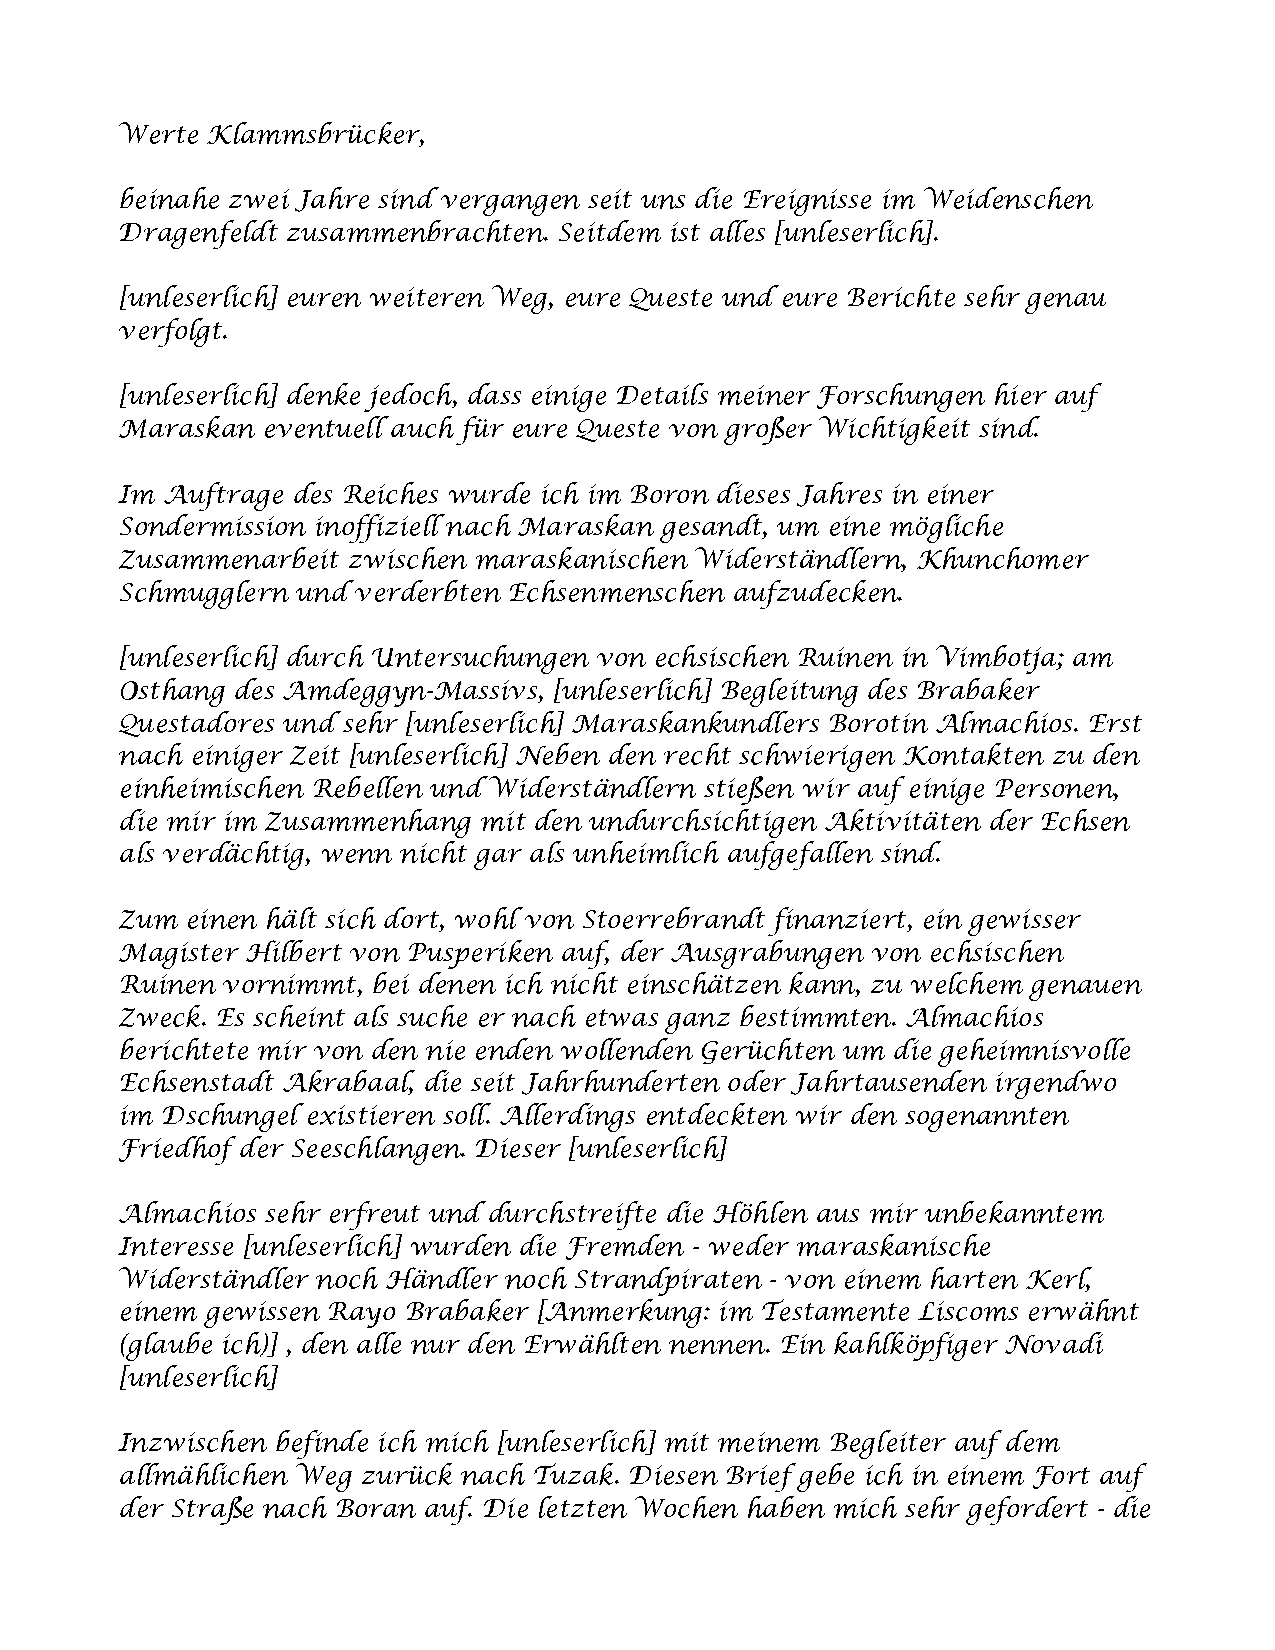
\includepdf[scale=0.9,pages=-]{handouts/part_2/pdg_brief_delian.pdf}

\includepdf[scale=0.9,pages=-]{handouts/part_2/pdg_haftbefehl.pdf}
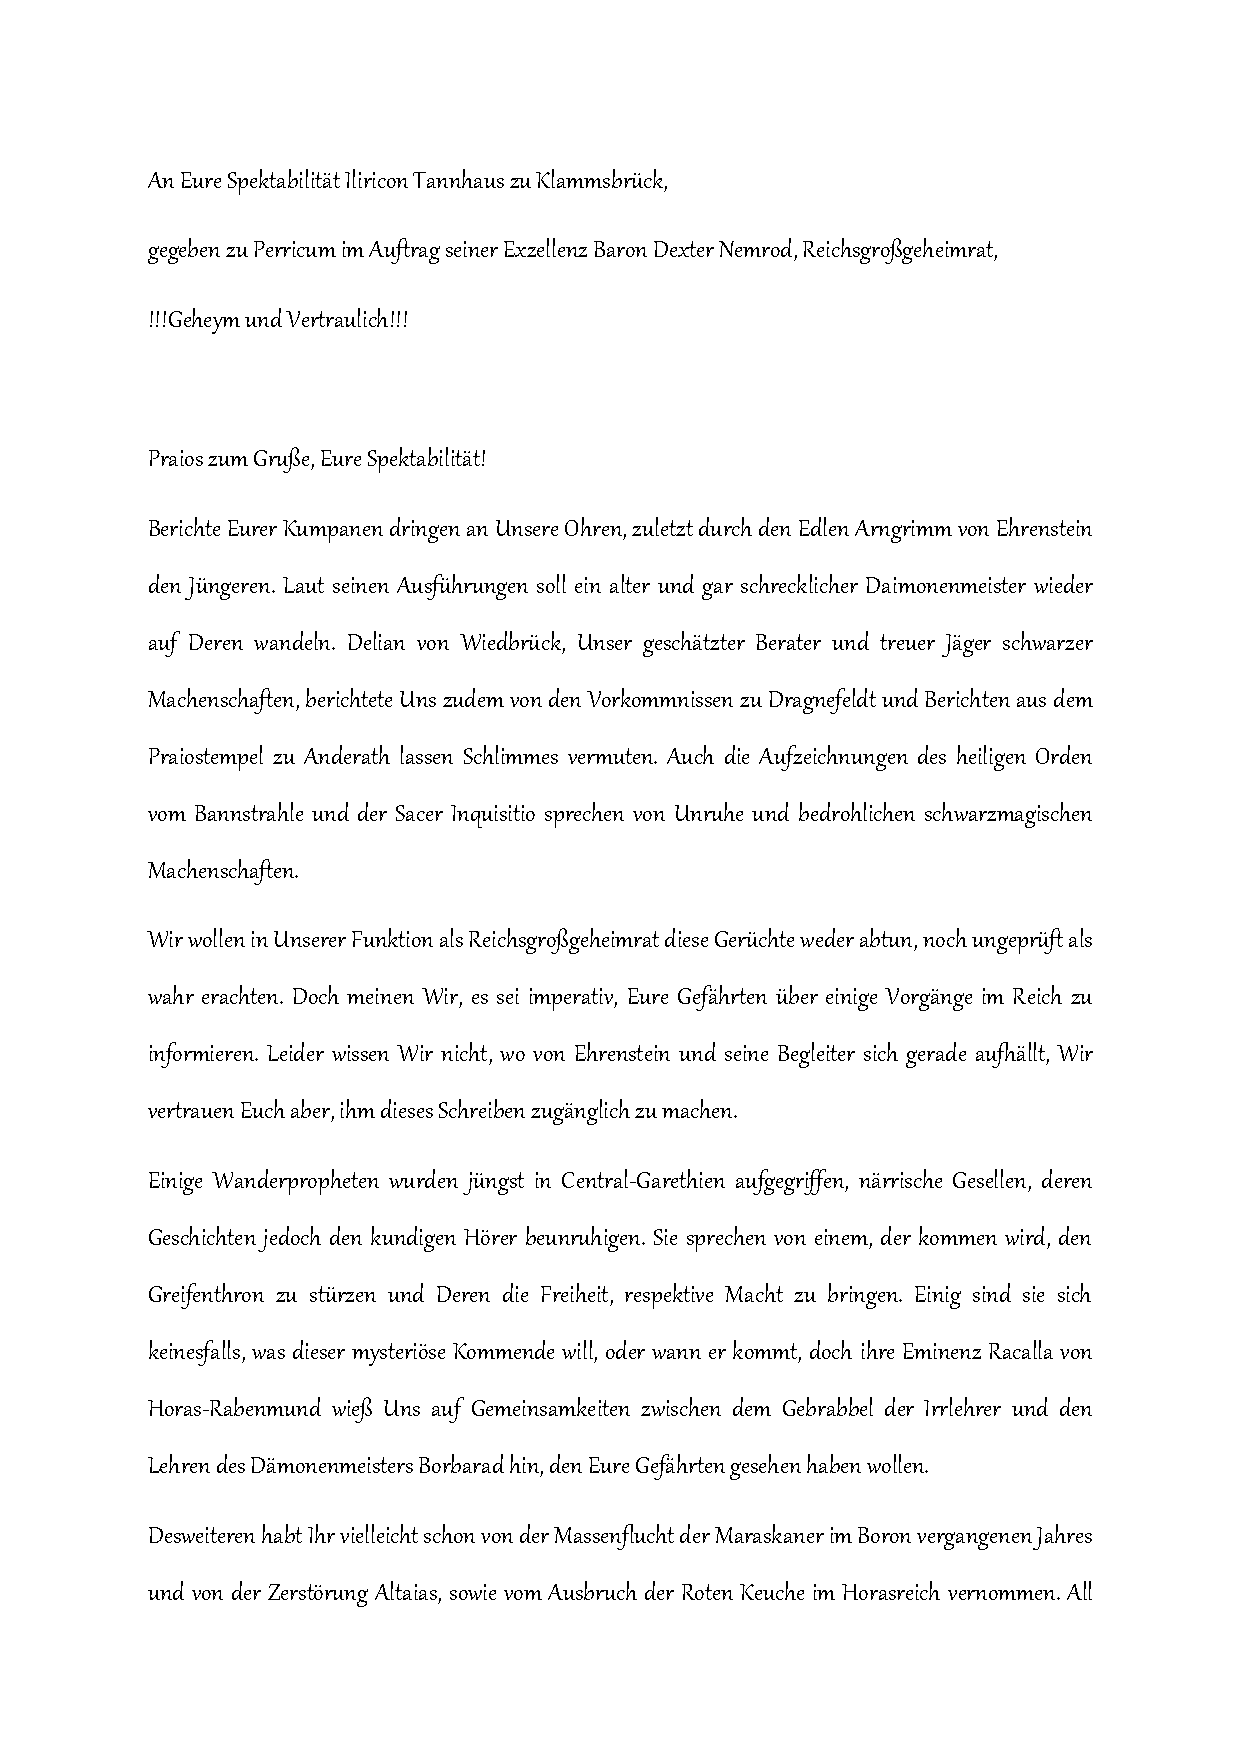
\includepdf[scale=0.9,pages=-]{handouts/part_2/siz_brief_dexter.pdf}



\part{Invasion der Verdammten}
\documentclass[11pt]{scrreprt}

\usepackage[utf8]{inputenc}
\usepackage[top=3cm,bottom=4cm,left=3cm,right=3cm]{geometry}
\setlength{\parskip}{6pt}
\setlength{\parindent}{0pt}

\title{Die Sieben Gezeichneten}
\subtitle{Invasion der Verdammten}
\author{Die Herren von Klammsbrück}
\date{2011 - 2016}

\begin{document}
\maketitle

\begin{abstract}
Die gesammelten Tagebücher der Helden der Dritten Dämonenschlacht, die ihr Leben gaben, um dem Dämonenmeister, dem Schänder der Sphären, dem Alveraniar des Verbotenen Wissens Einhalt zu gebieten.
\end{abstract}

\chapter{Euch zum Geleit}

\chapter{Bericht über die dreuenden Schatten}

\chapter{Pforten des Grauens}

\section{Geleitwort}


\begin{flushright}
Claas Völcker, Toronto, den 25.05.2025
\end{flushright}


\section{Die Tagebücher}

\end{document}


\part*{Handouts III}
\addcontentsline{toc}{part}{Handouts III}
\chapter{Texte aus der Vorbereitung}

\section{Ein Spionagebericht}
{\itshape
Diese Berichte scheinen Helme Haffax, Azaril Scharlachkraut, Arngrimm von Ehrenstein, und Travian von Rabenmund zu beschreiben.
}

``Wie steht es um das Südheer?'', fragt der große Mann in den Raum. Fackeln erleuchten ihn nur schwach und das unregelmäßige Licht wirft große Schatten an die steinernen Wände. Der hagere Magier erblasst, das Licht lässt ihn wie verhungert erscheinen: “D.. die G.. Gotongis sind in die 7. Sphäre zurück gefahren, Herr. Wir haben keine Informationen über das Verbleiben der Obristin von Perricums oder ihres Generalsstabs. Wir, wir müssen davon ausgehen, dass das alle magischen und exsphärischen Einheiten des Verbandes vernichtet wurden.” Er reibt nervös seine Hände und blickt sich um. Die anderen Gestalten im Raum bleiben regungslos und starren zurück, ihre Mienen verraten nichts. Kaum merklich nickt der große Mann und der Magier eilt aus dem Raum \dots

\dots In einem Schankraum, in einer düsteren Ecke sitzt eine wunderschöne Frau. Ihr edles Kleid, ihr hochnäsiger Blick und ihr vorsichtig geschminktes Gesicht machen deutlich, dass sie von Stand ist und doch sitzt sie ohne Begleitung oder Eskorte in einer Taverne. Die Atmosphäre ist gedrückt, das Licht erhellt den späten Abend nur schwach. Die Namenlosen Tage verbringt niemand gerne außerhalb der eigenen vier Wände.

Ein Schatten fällt auf die Frau und ihr maskenhaftes Gesicht verzieht sich zu einem dünnen Lächeln. Sie nickt zu dem freien Stuhl neben sich und dabei wird ein Blick auf ihre Ohren frei, auf spitze Ohren. “Habt ihr euch an die neuen Umstände gewöhnt?” fragt sie den Neuankömmling, eine Gestalt, die komplett durch einen langen schwarzen Mantel verhüllt ist. „Ja“, gibt dieser zurück und setzt sich . „Seid ihr sicher, dass sie kommen werden?“, fragt er langsam, als müssten sich seine Lippen noch an die Worte gewöhnen. Eine silberhelles Lachen ertönt, doch es klingt wie eine Glocke auf einem Boronsanger, „Wo sollen sie denn sonst hingehen“, fragt die Frau und blickt den dunklen Mann direkt an. ``Sie werden kommen, das verspreche ich euch, und wir werden auf sie warten...'' \dots

\dots Zwei Männer reiten über ein Schlachtfeld, um sie herum ertönt das Stöhnen der Verwundeten und die Schreie derer, die mehr gesehen haben, als sie sollten. Die beiden Männer scheinen das nicht zu bemerken, sie blicken auf die brennende Burg vor ihnen. Sie sehen sich sehr ähnlich, in ihrem prunkvollen silbernen Rüstungen, die die Zeichen der Schlacht tragen. Auf ihren Schildern prangen ein Wolf und ein Rabe und ihre Klingen sind noch rot vom frischen Blut vieler toter Soldaten.

``Die Thronräuber und Verräter fliehen wie die Ratten vor dem Feuer!'', meint der Jüngere mit dem Rabenwappen triumphierend, und richtet seinen Blick auf den Älteren neben ihm ``Bald werden wir vor den Mauern Wehrheims stehen und dann werden sie wissen, dass eine neue Ära angebrochen ist!'' Der Ältere blickt weiter grimmig auf das flammende Inferno und meint: ``Die Verräter und Ursupatoren werden büßen, für das was uns genommen wurde! Und das schon bald!'' Plötzlich wendet er seinen Kopf zu seinem Gefährten und fährt dann bestimmt fort: ``Du wirst verlangt.'' Der Rabenritter blickt ihn überrascht an und antwortet mit fester Stimme: ``Was immer ihr befiehlt, Herr, ich bin euer gehorsamster Diener!'' ``Es wird eine Jagd geben und die Legatin des Meisters verlangt einen Bluthund.'' Unterwürfig verneigt sich der Jüngere: ``Ich bin bereit für die Hatz.'' ``Folge dem Heer. Ihr werdet euch bald treffen. Und das Wild wird dir ganz besonders gefallen...'' \dots

\section{Die Trümmer von Kurkum}

Die Trümmer der mächtigen Wehrmauern und Gebäude Kurkums ragen schwarz vor Ruß in den Himmel auf. Die Luft riecht nach Rauch und Asche, das Knacken von schwelenden Balken dringt an euer Ohr. Das Tal ist still, tot, nach dem Lärm der Schlacht. Leises Schluchzen erklingt, eine alte Frau stöhnt verzweifelt als die Überlebenden den Tempel der Rondra verlassen. Wie ein Stück einer anderen Welt steht der Leuentempel da, wie eine Erinnerung an eine vergangene Zeit, unberührt von Schlacht ud Flammenmeer. Vielen um euch herum kullern Tränen über die Wangen und hinterlassen Furchen in dreckigen Gesichtern. Der beißende Geruch nach Rauch, der heiße Staub, all das lässt auch eure Augen tränen. Das stoze Volk der Amazonen, die hehren Soldatinnen der Rondra sind in die Hallen des Mythraelsfeldes eingegangen.

Rohana von Kurkum, die letzte Kriegerin der Feste, tritt zwischen euch. Ihr Harnisch ist verbeult und ihre Kleidung von Blut durchtränkt. Sie trägt einen tiefen Schnitt über ihre linke Wange und humpelt ein wenig. In ihrem bleichen Gesicht zeichnet sich Verzweiflung ab und in ihren kraftlosen Fingern hält sie ein zerbrochenes Schwert. Unter dem Dreck und der Asche erkennt ihr einen kunstvoll gearbeiteten Griff. Es ist das Schwert der Königin, zerbrochen durch den letzten Schlag des furchtbaren Dämons.

``Geht hinaus!'' flüstert sie mit letzter Kraft, ``Verkündet der Welt, dass Yppolita von Kurkum gefallen ist! Das Kurkum gefallen ist!''

\chapter{Ausarbeitung der Baronie}

{\itshape
Lieber Waldemar,

Ich habe hier einige Aufzeichnungen zusammen getragen, die einst die Chronik der Baronie hätten werden sollen. Ich hoffe, sie sind als Kontext für die Berichte der Gezeichneten nützlich.
}

\section{Grunewaldt: Geschichte}

Grunewaldt, ehemals Ebersberg, ist eine kleine Baronie im westlichen Tobrien. Nachdem der alte Verweser des Grafen, Baron von Stahlheim zu Ebersberg, seine Befugnisse überschritten und die Region maßlos ausgebeutet hat, eroberte der junge Jasper von Grunewaldt, ein Edler der Region, die Baronie und schlug den Söldnerhaufen des Stahlheimers. Der Edle wurde in der wirren Kaiserlosen Zeit von Graf Rondradan von Streitzig als Herrscher von Grunewaldt eingesetzt. Um den Göttern für die Wendung des Schicksals der Baronie zu danken beschloss der junge Jasper dem Praios eine Siegeskirche zu bauen. Diese Kirche verschlingt nun schon seit mehreren Jahren Unsummen, und langsam beginnen die Bauern der Region unmütig zu raunen.

Nach dem tragischen Tod des Jasper von Grunewaldt bei der Jagd, fiel die ertragreiche Baronie an den Herrn zurück, da der verblichene keine Kinder hinterließ. Um Schulden beim Herzog von Tobrien auszugleichen, beschloss von Streitzig, diesem die Baronie zu vermachen, ein Entschluss, der ihm einiges an Überwindung abverlangte. Die Baronie wurde einem jungen Sprössling des Hauses Ehrenstein, Arngrimm dem Jüngeren als Lehen verliehen, der sich sofort an eine weitere Ausbeute der Minen und einen Ausbau der wirtschaftlichen Vormachtstellung machte. Viele der älteren Bewohner nahmen dies nicht gut auf; sie waren skeptisch wegen der großen Träume ihres Herren. Die jüngeren aber träumten genau wie Arngrimm von einer Heimat, die man in einem Zuge mit Ysilia, Warunk und Mendena nennen würde. Das bis dahin der Weg noch sehr weit war, ignorierten viele fröhlich.

Nach Arngrimms vorzeitigem Ableben beim Scharmützel von Tuzak war die Baronie wieder herrenlos und wurde von Ratsherr Eichmannsson im Name des Herzogs von Tobrien regiert. Nach der Rettung des Herzogs Bernfried in der Schlacht von Vierreichen, wegen der großen Verdienste um das Herzogtum in den Schlachten von Kurkum, Eslamsbrück und Vierreichen und wegen der Beschaffung der Hauer des Mendenischen Ebers erhob der Herzog den Edlen Ragnos vom Svelltal zu Klammsbrück in den Rang eines Barons zu Grunewaldt. Er sollte die Bewohne seiner neuen Baronie in die letzte Schlacht gegen den Dämonenmeister führen.

\section{Grunewaldt: Land und Leute}

Die Nähe der schwarzen Sichel mit ihren Silberminen und Steinbrüchen macht die Baronie einigermaßen ertragreich, obwohl sie inmitten einer armen Region liegt. Der Norden der Baronie ist größtenteils bewaldet und versumpft, der Süden hingegen ist zur landwirtschaftlichen Nutzung geeignet. Hier wird ein Großteil des Korns der Baronie geerntet. Die Minen im Westen brachten lange nur wenig ein. Während der kurzen Herrschaftszeit Arngrimms des Jüngeren von Ehrenstein wurden diese Minen jedoch deutlich vergrößert so dass kurz vor dem Tobrienkrieg der Handel zu florieren begann. 

Die Baronie hat drei größere Städte: Grunewaldt (ehem. Ebersberg), mit 530 Einwohnern die größte und wichtigste Stadt, Kornheim, mit 350 Bürgern das Getreidezentrum im Süden und Stahlheim, ehemals 600 Einwohner, heute noch etwa 200, der ehemalige Hauptsitz der Barone.

\section{Die Stadt Grunewaldt}
Die Stadt Grunewaldt ist die Hauptstadt der Baronie und zeigt dies auch offen und stolz. Durch Handel und Friede ist die Stadt sehr wohlhabend geworden und nennt sich trotz praktisch fehlendem Stadtrecht: Stadt. Das ist auch das Ziel dieser kleinen und kämpferischen Gemeinde. Aber man ist dem Herrscher Jasper trotzdem nicht abgeneigt gewesen, die Kleinbürger waren durchaus stolz, dass „ihr“ Edler die Baronskrone errungen hat. Auf den neuen Verwalter der Baronie blickt man mit typischer konservativer Skepsis, ist einer Neuerung aber nicht grundsätzlich abgeneigt.

Auf dem Weg zum Stadtrecht haben die Städter sich eine eigene „Verwaltung“ und die Befreiung aus der Leibeigenschaft erkämpft. Grunewaldt ist sozusagen Stadt mit dem Baron als Stadtherrn.

Wichtige Orte der Stadt sind der Marktplatz und die Burg. Dort befinden sich eigentlich alle wichtigen Gebäude. Einige Gewerbe und Handwerker haben sich dort niedergelassen. So findet sich dort das „Große Handelshaus und Lager“ welches für den Handel mit Silber und Stein zuständig ist und bescheidenen Reichtum erwirtschaftet hat. Auch ein Silberschmied und Schmuckmacher, weit über die Grenzen der Baronie hinaus berühmt hat hier seine Werkstadt, nebenbei ist er am äußerst lukrativen Silberhandel beteiligt.

\subsection{Gebäude und wichtige Orte der Stadt}

Das Garnisionshaus, welches ein größeres Haus nahe der Stadtmauer ist, bietet den Stadtbütteln einen Platz zum Schlafen, Gefängniszellen zum Festhalten von auffällig gewordenen Bürger und einen ausreichend großen Innenhof, der als Übungsplatz für die Büttel dient. Die meisten Büttel sind jedoch für ein ausreichend großes Handgeld bereit ein Auge zuzudrücken. 

\subsection{Tobimorahafen}
Der 25 Schritt lange seitlich in den Fluss hinein gebaute Holzdock mit dazugehörigem steinernem Hafenhäuschen, den die Bewohner liebevoll Hafen nennen, bietet kleinen Flussschiffen eine Anlegestelle für die Nacht und die Möglichkeit ihre Waren zu löschen und neue aufzunehmen. Da die Tobimora hier nur einen Bruchteil so groß ist, wie weiter unten an der Mündung bei Mendena, ist der Handel über den Fluss auch von geringerer Bedeutung, da größere Flusssegler können hier nicht anlegen können und somit nur der Transport von kleinen Warenmengen möglich ist. Und überhaupt trauen sich nur erfahrene Flussschiffer zu, die Stromschnellen bis zur nächsten größeren Stadt Ebelried zu meistern. Der Hafen liegt nicht innerhalb der Stadtmauern. Doch allein die Tatsache einen Tobimorahafen zu besitzen, steigert das Ansehen der Stadt gewaltig. Im kleinen Hafenhäuschen sitzt der Hafenverwalter Eberhard Karjensen zusammen mit den Handelsaufzeichnungen der letzten zehn Götterläufe und führt Buch über die eingehenden und ausgehenden Waren, sowie über die Zollabgaben. Er ist ein kauziger alter(60) Kerl, der die Handelsregister des Hafens beinahe auswendig kennt. Die zum Hafen zugehörigen Lagerhäuser stehen innerhalb der Stadtmauer.

\subsection{Marktplatz \& Händler}
Gleich mehrere reiche Händler haben sich am Marktplatz angesiedelt und verkaufen dort ihre Waren. Unter anderem der überregional bekannte Silberhändler, ein Steinhändler und ein Holzhändler.

Alle vier Wochen in den Sommermonaten findet hier ein überregionaler Markt für Güter aller Art statt, auf dem sowohl die Waldbauern, die nur selten in die Stadt finden, als auch alle Händler aus der Stadt, sowie vorbei reisende Händler ihre Waren anbieten.

\subsection{Tempel und Schreine}
\paragraph{Praioskathedrale}
Die Praioskathedrale wird als Siegeskirche für den Sieg der Grunewalder über die Stahlheimer gebaut und wurde vom alten Baron Jasper von Grunewaldtin Auftrag gegeben. Doch auch nach vielen Jahren Bauzeit steht zurzeit nur das Grundfundament und mit den nicht sehr üppigen Geldspritzen des Barons wird sich das nicht so schnell ändern. Doch dank des Bauvorhabens sind immer ein paar Priester des Praios, sowie ein paar Bannstrahler in der Stadt.   

\paragraph{Perainetempel}
Der Perainetempel ist die feste Vertretung der Perainekirche in der Region. Er liegt ein wenig entfernt vom Marktplatz, zwischen diesem und dem Stadttor. Tatsächlich lassen sich die meisten Perainegeweihten jedoch auf den Feldern im Süden der Stadt finden, wo sie den Bauern bei der Arbeit helfen und die Felder segnen. Doch auch wenn man mit einer Verletzung, einer Krankheit oder einem anderen Anliegen in den Tempel kommt, wird einem geholfen. Meist kümmert sich die alte Tempelvorsteherin Treunai Jolen von Reiherweiher um einen gleich persönlich, meistens beobachtet von mindestens einem der Novizen des Tempels. Mit ihrer freundlichen, unaufgeregten und beruhigenden Art ist sie sehr beliebt bei ihren Patienten. Dank ihres Alters hat sie viel Erfahrung, ist jedoch körperlich nicht mehr in der Lage lange auf dem Feld zu arbeiten. 

\paragraph{Boronschrein}
Der kleine Boronschrein liegt zwar innerhalb der Stadtmauern, jedoch in guter Laufnähe zum Boronsanger, der außerhalb der Stadt liegt. Er wird vom alten Borongeweihten Anshag Kohlmoor betreut, der auf seine alten Tage sein Leben der Erhaltung des Tempels und des Boronsangers gewidmet hat. Auf seine alten Tage hört er und sieht er nicht mehr gut und spricht mit kratziger Stimme. Sein Geist ist jedoch noch scharf. Er lebt von den Spenden der Bewohner. 

\paragraph{Firunsschrein}
Der Firunsschrein wird vom Jäger des Barons betreut. Er ist auch für die Opfer für den eisigen Gott verantwortlich. Nur selten kommt ein Firunsgeweihter vorbei um selbst Opferrituale abzuhalten. Der Firunsschrein ist direkt an der Stadtmauer gelegen und karg gehalten. Nur eine Statue aus Stein ziert den Schrein.

\paragraph{Ingerimmsschrein}
Der Ingerimmsschrein steht direkt neben der örtlichen Schmiede, denn er wird auch vom örtlichen Schmied und seinen Lehrlingen geführt. Wie bei den anderen Schreinen kommt ein Geweihter nur alle paar Monde vorbei.

\subsection{Die Burg des Barons}
Die Burg des Barons von Grunewaldtliegt verschiedenen Berichten zufolge gleichzeitig direkt neben der Stadt Grunewald, von zwei kleinen Flüssen eingerahmt und nahezu uneinnehmbar vom Fluss aus und nur schwer einnehmbar von der Stadt aus oder wahlweise auf einem der Hügel der Umgebung auch hier schwer befestigt aufgrund der Streitigkeiten mit den Stahlheimern. Die Burg ist nicht groß. Platz genug im Haupthaus für den Baron und seine Dienerschaft, die nicht sehr groß ist, einen kleinen Stall, einen Trutzturm, einen Brunnen und einer kleinen Kaserne für die wenigen Soldaten, aber sonst nicht viel.

\subsection{Schänken und Gasthäuser}
\paragraph{Burgblick:} Direkt am Marktplatz gelegen, ist das steinerne dreistöckige Gasthaus die erste Wahl am Platz. Im Schankraum verkehren die reichen Händler der Stadt und die Reisenden, die es sich leisten können. Auch halten hier die Ratsherren den Stammtisch ab, an dem sie sich die Sorgen und Fragen der Bevölkerung anhören. Die monopolähnliche Stellung schlägt sich auch auf den Preis nieder und so ist hier alles ein wenig besser, jedoch deutlich teurer. Norsold Neuenhag leitet die Schänke. Der untersetzte Mitvierziger mit gepflegtem Vollbart versteht es seine hohe Kundschaft zu unterhalten. Er hat viel Erfahrung in seiner Tätigkeit und schon Gasthäuser in Beilunk und Ysilia geleitet, bevor es ihn nach Grunewaldtverschlagen hat. Dementsprechend führt er seine 3 Mägde und 2 Knechte mit strenger Hand. Seine rundliche Frau ist eine begnadete Köchin und hat die Leitung in der Küche inne. Neben tobrischen regionalen Gerichten werden hier saisonal auch immer wieder exotische Spezialitäten angeboten. Nach den ersten harten Anfangsjahren läuft das Geschäft, auch dank der nach Klammsbrück durchreisenden Magier immer besser.

\paragraph{Zur Kathedrale:} Die neu neben der Kathedrale entstandene Schenke bietet der bürgerlichen Schicht und den anwesenden Verantwortlichen der Praioskirche einen großen Schankraum, in den man bei gelegentlicher Unterhaltung durch lokale Barden gemütliche Abende bei gutem Bier und zünftiger Mahlzeit verbringen kann, ohne, dass einem gleich der ganze Geldbeutel gelehrt wird. Die regelmäßig zusammentreffenden gutbürgerlichen Stammtische halten ihre konservative Meinung oft nicht zurück und kritisieren für den ganzen Raum hörbar die Magierakademie, um im gleichen Satz den verstorbenen Baron Grunewaldtfür das Errichten der Praioskathedrale zu loben. Die verwitwete Wirtin Nalle Trutzquell führt die Schenke mit viel Hingabe und Leidenschaft, seht zur Freude ihrer Gäste.
Tobimora-Schänke: In einer engen Gasse nahe der Stadtmauer befindet sich die Tobimora-Schenke. Hier verkehrt hauptsächlich die ärmere Bevölkerung der Stadt und natürlich der Teil, der nicht gesehen werden will. Bei verwässertem Bier, heruntergekommener Einrichtung und schlechter Beleuchtung werden Fremde hier nicht gerne gesehen. Nur selten muss der schmierige, hagere Wirt Leuegrimm Schafbühler die Schlüssel für seine beiden mit Spinnenweben verhangenen 6-Personen-Schlafräume herausgeben, da kaum jemand, der es vermeiden kann, sich in ein solches Zimmer einmietet. Oftmals starten hier Prügeleien, die jedoch schnell zu Ende sind, sobald die beiden von Wirt als Streitschlichter eingestellten, muskelbepackten Holzfäller eingreifen. 

\subsection{Die Wichtigsten Bewohner der Stadt}
\paragraph{Ratsherr Wulfgrimm Eichmannsson:} der ernannt „Ratsherr“, eigentlich ein bescheiden-reicher Händler mischt sich regelmäßig in die Geschäfte des Barons ein, um zu sehen: „Ob des da oben alles so mit rechten Dinge zugeht!“ Er gilt als gemütlicher, aber erzkonservativer Mann.

Seine drei Ratskollegen bilden einen Stammtisch in der Schenke Burgblick und hören sich regelmäßig die Beschwerden der Bürger an um sie dem Baron vorzutragen. Eigentlich müsste ml wieder gewählt werden, aber damit hat es keiner eilig.

\paragraph{Hauptmann Eichinger:} der charismatische, quasi unkorrumpierbare Hauptmann der Wache ist der eigentliche Held der Stadt. Seitdem seine Frau bei einem Überfall auf den Silberhändler unter unglücklichen Umständen ums Leben gekommen ist, lebt er fast nur noch für die Wache. Tag und Nacht verbringt er im Wachhaus und macht Pläne wie er gegen das mehr oder weniger organisierte Verbrechen vorgehen kann. Durch kluges Vorgehen hat er bereits einen großen Kreis an Freunden und Vertrauten und hat sich einen eigenes Informationsnetzwerk geschaffen, mit dessen Hilfe er die kleinen Verbrechen in der Stadt besser aufklären will. Er ist groß gewachsen, aber eher hager und 28 Jahre alt, jedoch schon Hauptmann der Wache, da er sich durch seine Verdienste für die Stadt hervorgetan hat, als der Posten vakant wurde. Er hat einen einnehmenden sympathischen Charakter und wird überall gerne gesehen, nicht allerdings bei Verbrechern. Er ist in die Heilerin verliebt.

\paragraph{Preslaw aus Festum:} der alte Alchemist ist geheimnisumwittert und lässt sich nur selten in der Stadt blicken. Man munkelt, er sei mit Dämonen im Bunde und kenne alle Namen der Dinge zwischen Alveran und den Niederhöllen. Die Akademie von Klammsbrück kennt ihn jedoch als guten Handelspartner und, wenn auch etwas kauzigen, Lehrer. Er stammt aus Festum und hat nach eigenen Aussagen in den Laboren des Roten Salamanders studiert.

\paragraph{Stine Weyhenmoos:} Die Heilerin, Barbierin, Baderin und in besonders seltenen Fällen auch Kurtisane von Grunewaldtist eine gutaussehende, junge Frau mit vielen Talenten. Gegen eine gute Bezahlung erfüllt sie viele Wünsche. Die rahjagefälligsten gibt es jedoch nicht gegen Bezahlung, sondern nur bei persönlichen Gefallen erfüllt. Sie ist Viertelzauberin. Sie findet den Hauptmann der Wache sehr gut, doch die beiden haben bisher noch nicht zusammengefunden.

\paragraph{Angela:} Die Kräuterfrau hat einen kleinen Laden namens Angelas Stübchen in einer Seitengasse. Dort verkauft sie Kräuter, Tinkturen und magisches Allerlei. Oft kommen die Magier von Klammsbrück hierher, um seltene Kräuter und Zutaten für ihre Tränke zu kaufen. Manche Dorfbewohner munkeln, dass sie eine Hexe sei, was tatsächlich zutrifft. Sie ist eine eher beleibte, intelligente Frau mit schulterlangen dunklen Haaren, bei der man das Gefühl hat, dass sie mit ihren dunklen Augen direkt in die eigene Seele blicken kann. Ihrem Gesicht kann man kein Alter wirklich zuordnen, aber den Laden scheint sie seit mindestens 20 Jahren zu besitzten.

\section{Die Gemeinde Kornheim}

Etwa zwei Tagesreisen von Grunewaldtentfernt liegt Kornheim, eine Ansiedlung von weit verstreuten Höfen die hauptsächlich Getreide, aber auch andere landwirtschaftliche Erzeugnisse, wie Äpfel, verschiedene Gemüsesorten und seit neuestem auf ein paar wenigen ausgewählten Feldern auch bornländische Kartoffeln anbauen. Innerhalb der etwa 150 von insgesamt 350 Bewohnern enthaltenen Palisaden befindet sich zentral eine kleine Kapelle, in der sich ein Peraine-Schrein befindet, dem die meiste Zeit des Jahres über mindestens einer der 3 Peraine-Priester aus der Stadt beiwohnt, sowie ein Phex Schrein. Des Weiteren sind dort die Kornkammern befindlich, sowie die Häuser der Bauern, die die Felder um die Stadt herum bestellen. Im großen Haus des Dorfvorstehers Wulf Weidenhude ist immer ein Platz für einen Reisenden und abends versammelt sich das halbe Dorf im großen Versammlungsraum, um Geschichten zu lauschen, Klatsch und Tratsch auszutauschen und um die Bewohner der um das Dorf herum liegenden Höfe zu treffen.

Jedes Jahr nach der Ernte findet in Kornheim ein großer Markt statt, an dem die Bauern der Umgebung ihre Waren überregional verkaufen. Viele Nachbarbaronien stocken ihre Getreidevorräte auf diesen Markt auf.

\subsection{Personen}
Wulf Weidenhude: mittelgroßer etwas beleibter rothaariger Mann mit Vollbart, 38 Jahre alt, lebt mit Frau und Kindern im großen Haus. Ihm liegt das Wohl des Dorfes sehr am Herzen, wie auch die althergebrachten tobrischen Traditionen. Seine Ansichten verteidigt er stur wie ein Zwerg und bei seiner Rechtschaffenheit macht er den meisten Praiosgeweihten Konkurrenz. Dies führt auch immer zu kleinen Zwisten mit den Magieschülern der Klammsbrücker Akademie, wenn sie auf dem großen Markt Nachschub für die Akademie kaufen.

\section{Stahlheim}
In der größtenteils noch immer verwüsteten Stadt, geht der Wiederaufbau nur langsam voran. Die etwa 150 Bewohner, die sich hier wieder angesiedelt haben sind hauptsächlich ehemalige Bewohner. Vor der Stadt betreiben sie ein wenig Landwirtschaft, Handel betreiben sie kaum, da alle Händler, die was auf sich hielten, ins zwei Tagesreisen entfernte Grunewaldtabgezogen sind.

\section{Steinbruch}
Der Steinbruch liegt etwa drei Tagesreisen von Grunewaldtentfernt in einer mittelgebirgsartigen Region. Er ist mittlerweile recht groß geworden und wird immer noch von einer Holzpalisade eingezäunt. Aus ihm wird vor allem die Praioskathedrale versorgt, jedoch auch die restlichen Bauten, bei denen Steine gebraucht werden. Etwa dreißig Arbeiter arbeiten hier, sie kommen in Holzbaracken unter. Alle drei Tage bewegt sich eine Schlange von Wagen den gut ausgearbeiteten Feldweg nach Grunewaldthinab. Zwar gäbe es einen kürzeren, jedoch würde dieser direkt durchs grüne Moor führen. Im Steinbruch hat ein Vorarbeiter des Verwalters der Baronie die Aufsicht, da der Steinbruch der Baronie gehört.

\section{Silbermine}
Seitdem der ehemalige Baron Arngrimm von Ehrenstein mithilfe der Magierakademie die Silbermine ausgebeutet hat, ist die Anzahl der Minenarbeiter stark gesunken. Doch der ehemalige Söldner Aytan ibn Feqadir hat sein Glück gesucht und gefunden und hat einige Meilen vom ehemaligen Fundort entfernt eine weitere Silbererzader gefunden. Zusammen mit fünf ehemaligen Minenarbeitern und dem Zwerg Brodrosch Sohn des Cobaltosch, der sich auf der Durchreise befindlich, spontan dazu entschlossen hat, bei dem Projekt mitzumachen und sein Wissen im Bergbau mit einfließen zu lassen, baut er dort das Silbererz ab, welches er an den bekannten Silberschmied und -Händler in Grunewaldtverkauft. Regelmäßig wird die kleine Karawane, die zusätzlich mit vom Silberschmied angeheuertem Söldern verstärkt wird, von den Wilderern überfallen, jedoch ohne größere Erzverluste. Dass diese Überfälle keine Zufälle sind, wissen Aytan und die Wilderer allein, da diese ein Abkommen geschlossen haben, um das Silber mit Gefahrenaufschlag teurer verkaufen zu können.

Die Mine ist durch eine massive Holztür geschützt. Innerhalb der umzäunenden Palisade befindet sich außerdem ein etwas größeres Holzhaus, in dem die Männer schlafen, essen und in dem das Erz verwahrt wird. Da die Mine etwas abgelegen in den Bergen liegt, ist sie nur durch einen kleinen Trampelpfad zu erreichen.

\subsection{Personen des Steinbruchs}
\paragraph{Aytan ibn Feqadir:} Männlich, 32 Jahre alt, Wohnort: an der Silbermine, Familie: keine in der Baronie, mittelgroßer drahtiger Tulamide, mit an den Schläfen ergrauendem schwarzem Haar, seine Gerissenheit als Söldner hat er eins zu eins auf sein Händlerdasein übertragen. Alles, was ihm zum Vorteil gereicht ist ihm recht, solange es kein höheres Verbrechen ist. Nach außen hin sehr nett und zuvorkommend, eher bescheiden. Ziele: Aufbau eines Vermögens, Aussorgen. Ängste: von Hauptmann Eichinger erwischt werden, mit dem er sich angefreundet hat, ihm aber ungerne erklären wöllte, dass er im Konflikt mit dem Gesetzt steht. Er ist immer noch ein begabter Kämpfer mit dem Säbel.

\paragraph{Brodrosch Sohn des Cobaltosch:} Männlich, Erzzwerg, 96 Jahre alt, Wohnort Silbermine, Hauptverantwortlich für die Silbermine in Sachen Abbau und Minensicherheit, Familie lebt in Xorlosch, für einen Zwerg recht groß, grummeliger Zeitgenosse, der sich am liebsten über Minen, Erz und dergleichen unterhält, guter Saufkumpan, geht zweimal im Jahr in die Schenke Zur Kathedrale, Wirtin gibt ihm immer kostenlos Bier, weil er guter Stimmungsmacher ist und die Taverne immer voll ist an diesen Abenden. Ziele: ein wenig Gold kann nie schaden, gutes persönliches Verhältnis zu Aytan. 

\section{Das grüne Moor}
Ein Moor Firun von Grunewaldtgelegen. Es beherbergt Sumpfranzen und ist bis auf ein paar vorgegebene Feldwege lebend und ohne Begegnung mit dem heimischen Sumpfranzen  kaum zu durchqueren. In dem Moor haust der verrückte Eitel Windkuppe, der sich anscheinend mit den Sumpfranzen angefreundet hat und manchen sich im Sumpf verlaufen habenden den Weg aus dem Sumpf weißt. Andere überlebten nur knapp und meinten in der Fern das Gelächter eines Mannes gehört zu haben. Über seine Vergangenheit ist nichts bekannt und wenige haben ihn je zu Gesicht bekommen. 

\subsection{Die Waldbauern}
Die Waldbauern sind mehrere auf Höfen im Wald verteilte Bauernfamilien, die Schafe und Rinder auf ihrem Wiesen weiden lassen. Sie kommen zum jährlichen Markt in Kornfeld und zu den Märkten in Grunewaldt. Manche stellen auch Holzkohle her. Über die Waldbauern erzählt man sich so manches unheimliches und sie sollen eher dem Sumukult der Druiden als dem wahrhaftigen Glauben der Zwölfe anhängen.

\section{Wirtschaft der Baronie}
Die Baronie erwirtschaftete in den letzten Jahren in einem Götterlauf nach Abzug aller Steuer etc. 1500 Dukaten Reingewinn. Unter Jasper von Grunewaldt floss ein Großteil dieses Geldes in den Bau der Praioskirche, etwa 500 D, und noch einmal so viel jedes Jahr auf die Nordlandbank als Rücklage. Die letzten 500 Dukaten zahlen das Leben des Barons, weshalb man zwar nicht sagen kann, dass er im Luxus lebt, aber auch nicht in bitterer Armut. Viel zusätzlich über sein Brot und Leinen konnte er sich allerdings nicht leisten.

Die Einnahmen der Baronie kommen nach wie vor zu großen Teilen aus dem Kornhandel und dem Hofzehnt, der bei allen Bewohnern der Baronie erhoben wird. Seit Argrimms Reformen gewinnt auch der Silberhandel und der Steinhandel deutlich an Bedeutung und immer größere Summen werden an den Baron abgeführt.

\section{Klammsbrück}
\subsection{Das Leben auf Klammsbrück}

„Aufstehen!“, dröhnte es durch die kleine Kammer. Stöhnend richtete Waldemar sich auf und blinzelte verschlafen. Die Kammer war durch die kleinen Fensterschlitze nur diffus erleuchtet und undeutlich konnte er die kleine, drahtige Gestalt in der Tür erkennen. Es war natürlich der Lehrer Erwen, ein Meister im Quälen von verschlafenen Schülern. Die Luft war erstaunlich kühl für Ende Praios und Waldemar fröstelte es leicht, während er sich langsam umblickte. Die vier anderen Schüler, die mit ihm in einem Raum schliefen, waren auch gerade dabei sich den Schlaf aus den Augen zu reiben oder verkrochen sich in ihren dünnen Decken. „Aufstehen Jungs!“, dröhnte Erwens unerbittliche Stimme noch einmal durch den Raum. „Praios Scheibe schaut schon auf euch herab und ihr liegt faul herum. Ihr habt Glück das Meister Calhadril nicht hier ist, der würde euch aber Beine machen. In zehn Minuten erwarte ich euch unten.“ Und mit diesen Worten drehte sich der junge Lehrer um und verschwand in dem langen Gang. Zurück blieben fünf müde Jungen im Alter zwischen elf und sechzehn Jahren, die sich alle irgendwo auf dem Weg zwischen Schlaf und diesseits befanden.

Waldemar wusste, dass man Erwen besser gehorchen sollte, vor allem am Morgen. Der Geweihte der Hesinde war berühmt-berüchtigt für seine schlechte Laune in den frühen Morgenstunden. Vor einer Woche hatte er den jungen Falkenhardt mit einem vollen Eimer Wasser geweckt. Der Arme hatte nur versucht nach einem langen Abend noch ein wenig Schlaf zu bekommen, aber Erwens Sternkundelektionen waren dem Lehrer wichtiger gewesen. Tropfnass und nur mit einem dünnen Mantel bekleidet, musste der jüngste Sohn des Barons von Grunewaldt herauf auf den Hauptturm steigen. Hesinde sei Dank war es eine laue Hochsommernacht gewesen, ansonsten hätte er sich den womöglich Tod geholt und wochenlang im Bett gelegen.

Waldemar wollte nichts riskieren und stieg deswegen schnell von seinem schmalen Nachtlager. Geschwind schlüpfte er in das lange, braune Gewand, das Pflicht für die Schüler der Schule von Klammsbrück war und eilte zur Tür. Falkenhardt hatte die Schlafkammer schon vor ihm verlassen, offenbar wollte auch er nicht noch einmal mehrere Nächte in einem nassen Bett schlafen. Die beiden eilten den langen Gang hinab, fest in der Absicht, dem Lehrer keinen Grund zur Klage zu liefern. Die unausgesprochene Drohung ohne Frühstück den Tag beginnen zu müssen, stand bedrohlich in der Luft. Vor den Fenstern, die leider nicht mit Glas, dafür aber mit schweren Fensterläden ausgestattet waren, zeigte sich ein atemberaubender Sonnenaufgang am anderen Ende des Tals von Klammsbrück. Praios Scheibe hatte sich schon über die Gipfel der umliegenden Berge gequält und tauchte das Land in rot goldenes Licht. Es  blendete Waldemar für einen Augenblick, tat seinem verschlafenen Geist jedoch sehr gut. Langsam schüttelte er die letzte Müdigkeit ab und blickte sich noch einmal um. Hinter ihm schlichen die letzten drei Schlafmützen aus der Kammer, die hochtrabend „Schlafsaal der Knaben“ genannt wurde. Die drei waren allesamt jünger als Waldemar, der als Ältester schon den illustren Rang eines Studiosus bekleidete.

'Sonderbar', dachte er sich, 'meine Brüder schuften jetzt schon im Stall oder auf dem Feld und ich grummle über Aufstehen mit dem Sonnenaufgang.' Fünf Jahre war es her, dass der Magier Iliricon das große Bauernhaus seiner Eltern betreten hatte. Er war damals elf, der jüngste von fünf strammen Burschen und sehr eingeschüchtert vom hohen Besuch. Man hatte sich im Dorf schon von den mächtigen Männern erzählt, die eine Burg im Norden der Baronie in Besitz genommen hätten und dem Baron so lange eingeheizt hätten, mit Wort und Zauberspruch, bis er ihnen gestattete, dort zu verweilen. Auch fünf andere Versionen der Geschichte kursierten in der Gegend, alle mehr oder weniger fantastisch. Die Männer, zwei Magier und einige Begleiter, hätten den Bau der Kathedrale in Grunewaldt verhindert oder sabotiert, manchmal auch gerettet. Inzwischen kannte Waldemar natürlich die Wahrheit und konnte nur noch über die verbrämten Gerüchte lachen die sich um Magister Temyr ibn Sahid und Iliricon Tannhaus rankten.

Die Wahrheit war, dass die Beiden zusammen mit dem Geweihten Oleg Sjepsen, dem Zwerg Korscho und dem Bornländer Rahjan als Karawanenbegleitung nach Grunewaldt gekommen waren. Sie beförderten teures Glas für die Fenster der Kathedrale, die in der Nähe der Stadt gebaut werden sollte. Als ihr Dienst für den Händler erledigt war, bat der Herr von Grunewaldt, Baron Jasper, die Fünf einige seltsame Vorkommnisse beim Bau zu untersuchen. Die Reisenden fanden heraus, dass der alte Baron, der Herr von Stahlheim, für die Sabotage verantwortlich war. Er hatte es Jasper nie verziehen, dass dieser ihm wegen seiner Unterdrückung der Bauern mithilfe von Kunibald von Ehrenstein gestürzt hatte. Die Magier und ihre Begleiter stellten den Verbrecher in seiner Burg in den Bergen, die vorher nie gefunden worden war und machten ihn den Garaus. Zum Dank übergab ihnen Jasper von Grunewaldt die desolate Festung und nahm sie als Junker und Vasallen auf.

Inzwischen war aus der Ruine ein stattliches Gut geworden. Zwei Bauernfamilien hatten das Tal bezogen und versorgten Herrn und Besatzung der Burg. Doch nur Junker zu werden, gefiel den hohen Herrn nicht. Durch mehr oder weniger legale Methoden waren sie an genügend Bücher gekommen, um eine ganze Bibliothek zu errichten. Bis an die Zähne mit arkanem und weltlichem Wissen gerüstet, hatten die Beiden, zusammen mit ihrem neuen Freund Calhadril Ignisfulgur, vor dem Gildenrat der Grauen plädiert, eine Schule für magisch Begabte in Tobrien errichten zu dürfen. Nach einigem Zögern und Zähneknirschen wurde ihnen dies unter der Auflage gewährt, kein eigenes Akademiesigel führen zu dürfen. Erst wenn sie bewiesen hätten, dass sie der hohen Würde der Spektabilität würdig seien, wäre der Gildenrat bereit, sie in ihren Rängen Willkommen zu heißen.

„Waldemar, du träumst schon wieder!“ Mit einem Mal befand der junge Magier sich wieder im hier und jetzt. „Du kommst am Ende doch noch zu spät zum Morgenmahl!“ Falkenhardt hatte den Kopf angewinkelt und blinzelte Waldemar genervt an: „Erst rappelst du dich endlich einmal pünktlich aus dem Bett und dann stehst du einfach in der Gegend rum, anstatt dich zu beeilen.“ Der Gescholtene schüttelte kurz den Kopf und eilte mit fliegendem Gewand los, um nicht doch noch zu spät zu kommen. Der kleinere Baronssprössling rief ihm hinterher: „Hej, das hieß nicht, dass du einfach wegrennen...“ Aber Waldemar war schon am Treppenhaus und eilte die ausgetretenen Steinstufen herab. In der geräumigen Halle der Burg brannte schon ein prasselndes Feuer und die meisten anderen Bewohner der Burg saßen an ihren Plätzen. Waldemar wollte sich gerade dazusetzten, als ihn eine starke Hand schmerzhaft im Genick packte. „Was sind die obersten Tugenden eines Ritters?“, fragte eine brummige Stimme. Waldemar antwortete sofort: „Ehrlichkeit, Tapferkeit, Gehorsam, Mut... Weisheit...“ Er stockte. „Und weiter, Bürschchen?“, fragte die Stimme etwas barscher. „Pünktlichkeit gehört meines Wissens nicht dazu“, antwortete der Schüler trotzig, „ Herr Sjepsens, währt ihr so freundlich und würdet mich zum Essen lassen? Ich bin nämlich kein Knappe und deshalb kann mir das Rittertum auch...“ Der Mann, der ihn festhielt, lachte einmal kurz und schlug ihm dann seine mächtige Pranke auf die Schulter. Waldemar keuchte. „Gut gekontert, Bürschchen, aber auch ihr Zauberstabschwinger müsst ein wenig Anstand lernen. Und Pünktlichkeit ist keine ritterliche Tugend, aber dennoch eine Tugend.“ Dann drehte der bärbeißige Ritter sich um und lachte erneut, als er in Falkhardt sein nächstes Opfer die Treppe herunter eilen sah. Panik stand dem Kleinen ins Gesicht geschrieben, als der große Mann mit fiesem Lächeln auf ihn zu stapfte.

\subsection{Buch der Burg Klammsbrück}

Das Vermögen der Herren zu Klammsbrück vor Borbarads Verkörperung
\begin{itemize}
    \item Barvermögen: 1700 Dukaten in Gold und Wechselbriefen
    \item 25 Stein Mindorit (laut Herrn Temyr 2500 - 3000 Dukaten wert)
    \item Alchemistische Ingredienzen im Wert von circa 100 Dukaten
    \item 8 persöhnliche Siegelringe mit Initialien und dem Wappen Klammsbrücks bzw. Abänderungen desselbigen
    \item 1 Edelstein, laut Herrn Temyr der Karfunkel eines Drachen, Geschenk von Teklador
    \item Bibliothek der Herrn Magi:
    \begin{itemize}
        \item Im Giftschrank:
        \begin{itemize}
            \item Arcanum (gekürzt)
            \item Codex Dimensionis 
            \item Astralen Geheimnisse (ungekürzt!)
            \item Codex Septasphaericum (Khunchomer Original)
            \item Vom Leben in seinen Natürlichen und Übernatürlichen Formen (stark gekürzt)
            \item Borbarads Testament
        \end{itemize}
        \item Zur freien Einsicht
        \begin{itemize}
            \item Annalen des Götteralters - Kaiser Retho Ausgabe
            \item 4 Bücher der Schlange aus einem nahegeliegnen Hesindetempel, Abschrift von Herr Erwen, befassen sich mit Philosophie, Theologie, Rhetorik und Logik
            \item 20 Bücher über die Combativa, die Transformatio und eines über die  Arkanogenese
            \item 30 Bücher über Land, Leute und Geschichte Aventuriens (erworben von Iliricon Tannhaus)
        \end{itemize}
    \end{itemize}
    \item Aus dem Besitz des Liscoms von Fasar:
    \begin{itemize}
        \item 1 Tiegelchen Schlafgift
        \item 2 Tiegelchen Athrax
        \item 1 Ampulle Omaris
        \item 1 Ring aus Eisen mit Onyxen und Boronssymbolen, als Artefakt zum Eindringen in Träume identifiziert
        \item 1 Amulett, eine dämonische Fraze zeigend (nicht analysiert)
        \item 1 Amulett, trägt laut Calhadril ein antimagisches Sieglum
    \end{itemize}
\end{itemize}
\subsection{Bewohner der Burg und der Ländereien:}

\paragraph{Gernot von Klammsbrück \& seine Frua Praiogard (Vogt \& Vogtin)}
Aufrichtige Seelen, die nun etwa 60 Götterläufe zählen. Der alte Gernot kümmert sich mit Fleiß und einer wahrhaft phexgefälligen Genauigkeit um die Finanzen des Lehens, während seine Frau die gute Seele der Burg ist, die für jeden als Ansprechpartnerin fungiert und die Küche betreibt.

Gernot ist ein hagerer alter Mann, der seinen Lebensabend in Ruhe verbringen will. Als ehemaliger Kämmerer der Herren von Stahlheim wollte er nicht länger in der Stadt Grunewaldt wohnen und verrichtet nun sein Handwerk auf Klammsbrück, wo ihn sowohl die Bewohner der Burg, als auch die Bauern und Jäger respektieren und schätzen gelernt haben (Typ: Albert [Batman]).

Seine Frau ist eine quirlige alte Dame, untersetzt mit einigen Steinen zu viel auf der Hüfte, die das Gegenteil ihres Mannes zu sein scheint. Der Garten der Burg ist ihr ein und alles, dort lässt sie selbst Iliricon nur unter ihrer Aufsicht ernten. Dem Geweihten Toran jedoch bringt sie ein Mischung aus Respekt und mütterlicher Fürsorge entgegn. Hätte sie Söhne gehabt, so wären diese natürlich zur Perainekirche geschickt worden. (Typ: Mrs. Sprout [Harry Potter])

\subsection{Die Baueren:}
\paragraph{Familie Wulfenbruck, deren beiden Söhne Klammsbrücks Wachmannschaft sind.}
Die Familie Wulfenbruck hat ihr Land während des Zuges der Oger vor 15 Jahren verloren. Nachdem sie sich mit ihren beiden damals noch sehr jungen Söhnen als Tagelöhner entlang der Tobimora bei verschiedenen Fischern und Schiffern durchgeschlagen hatten, halfen sie auf den Feldern von Kornheim als Tagelöhner aus. Als die Herren von Klammsbrück neue Pächter suchten, waren sie bereit, alles aufzugeben, um im Tal von Klammsbrück zu arbeiten.

Folgende Wulfenbrucks nennen Klammsbrück ihr Zuhause: Oma Wulfenbruck, Vater \& Mutter Wulfenbruck, 2 ältere Söhne, drei jüngere Töchter

\paragraph{Familie Treublatt, deren Sohn Alrik Klammsbrücks umstrittener Torwächter ist.}
Die Familie Treublatt wiederum verpachtet selber einige Höfe in Kornheim und ist ein Clan, der in der ganzen Baronie einiges an Einfluss hat. Der Patriarch der Familie Wulfenhardt Treublatt, ist ein Kaufmann in Grunewaldt, während seine Kinder, Enkel und Neffen, beziehungsweise Nichten auf verschiedenen Höfen das sagen haben. Der alte Treublatt war auch der Berater der letzten Barone von Grunewaldt und machte sich als dieser nicht nur Freunde.

Folgende Treublatts wohnen in Klammsbrück: Vater (Sohn des alten Treublatts) \& Mutter Treublatt, fünf Söhne (zweitjüngster ist Alrik) und drei Töchter

\subsection{Die Lehrmeister}
\paragraph{Iliricon Tannhaus, stellv. Spektabilität der Akademie, Magister Transformationes}
Magister Magnus Tannhaus, stellvertretende Spektabilität zu Klammsbrück, ODL, ist ein meisterlicher Verwandlungsmagier, der einst zur Abenteurergruppe der Herren von Klammsbrück gehörte. Nachdem seine Mutter im Orkensturm ermordet wurde, geriet er in die Fänge des Erzdämons Blakharaz und konnte nur durch den heldenhaften Einsatz seiner Kumpanen gerettet werden. Heute lebt er sehr zurückgezogen, über seine Zeit hinaus gealtert, in Klammsbrück und verwaltet dort die Akademie. Sein zweites Projekt ist das Sammeln von allerlei Informationen zu Borbarads Rückkehr, vor allem die Erlebnisberichte der Gezeichnete selbst. Aus ihren Tagebüchern und Erzählungen schreibt er eine Chronik.

Tannhaus trägt trotz seines jungen Alters von knapp 35 Götterläufen tiefe Falten im Gesicht, die seine elfenhaften Züge etwas verblassen lassen. Er ist jedoch nach wie vor ein guter Stabkämpfer und kompetenter Magus.

\paragraph{Falk Kornberg, Magister Combatitivus}
Magus maior Kornberg ist ein alter Freund Iliricons aus Lowangen. Er forschte mit einer kleinen Gruppe lange Zeit in den Elfenwäldern, um den Verwandlungen der Elfen hinterher zu spüren, allerdings vertrieben ihn diese vor drei Jahren, als er eine Sippe beim Salasandra störte. Da Lowangen tief im orkischen Gebiet lag, wollte er nicht dorthin zurück, sondern begab sich ins Raulsche Reich, wo er sich in Ysilia als Lehrmeister bewarb. Man verweigerte ihm jedoch eine Anstellung, da man keinen Dozenten für Verwandlungen benötigte und außerdem keinen Graumagier in den eigenen Reihen aufnehmen konnte. Der Magus, der sich aber zum Lehrer berufen sah, nachdem seine Forschung misslungen war, wurde nach Klammsbrück geschicjt, um dort bei der Lehre zu helfen.

Kornberg ist Mitte 30 und ist groß und schmal wie ein Greifvogel. Seine markante Hakennase hat ihm den Spitznamen Adlernase eingebracht, was ihn regelrecht zur Weißglut bringen kann.

\paragraph{Arn Wulfgardt, Adeptus minor combatitvus}
Arn Wulfgard ist ein hochgewachsener kräftig gebauter Mann (der fast die Statur Olegs heran reicht)
Das dunkelblonde Haar trägt er aus praktischen Gründen immer kurz, in völliger Missachtung des Codex. Der Bart ist stets ordentlich gestutzt. Und das Gewand ordentlich gefaltet (Da schlägt die adlige Früherziehung durch.)
Wenn auch vollkommen von Sich und seinen Fähigkeiten überzeugt, ist er ein freundlicher Zeitgenosse, der gerne bereit ist die Anderen an seiner Weisheit teilhaben zu lassen.
Trotz seiner Abstammung hat ihn die ganze Etikette, Weltgewandheit und Allgemeinwissen nie groß interessiert. Die Nachmittage verbrachte er lieber mit dem Schnizen an Holzstöcken (wo er ein erstaunliches Können entwickelte) und seine Berufung zur Magie war der Einstieg in das Abenteuer seines Lebens.

Mit Faszination begeistert er sich für Sagen und Legenden, alles was die Historie an Schlachten zu bieten hat. Aus reinem Interesse hat sich einiges an Wissen über die Kriegskunst angeeignet. Wenn man Fragen im Heraldischen Bereich hat, heute, wie in der Vergangenheit, ist man bei ihm an der richtigen Adresse.
Die Begeisterung am Kampfe setzt sich auch Körperlich fort. Mit dem Stab versteht Arn es vorzüglich um zu gehen, auch wenn sein Stil wenig elegant ist, ist er doch um so effizienter, und mit einer Liebe für's Detail, entgeht seinen kalt blauen Augen, nicht der geringste Fehler seines Gegners.
Seine Spezialität im arkanen Bereich, sind die Zauber: Armatrutz, Gardianum, Horiphobus, Ignifaxius und Paralysis. In der Analyse (Odem und Analysis) ist er ausreichend bewandert und auchden Unitatio beherscht er gut.
Das alte Tobrische Blut (vlt. mit der ein oder anderen Bornländischen Wurzel) prägt sich vor allem durch ein überdurchschnittliches Vertragen alkoholischer Substanzen, in kalten Wintermonden, aus. 

\paragraph{Tanja Winterkalt, Adepta minor transformationes}
Adepta Winterkalt hat zusammen mit Arn Wulfgardt ihre Prüfung vor einer Sonderkomission des Pentagrammatons zu Punin abgelegt und damit den Grundstein gelegt, dass Klammsbrück eine richtige Akademie werden konnte. Sie ist heute neben Iliricon eine Hauptinstruktorin an der Akadmie und kümmert sich neben ihrem eigentlichen Feld, der Transformation, vor allem um die etwas in den Hintergrund gerückte Hohe und Niedere Alchemie, also um Trankherstellung und Arkanogenese. Ihr momentanes Projekt ist die Herstellung von Pentagramma-Artefakten zusammen mit der Akademie zu Ysilia.

Winterkalt ist ein junge hübsche Frau (Anfang 20) mit Sommersprossen, die ihr Haar gerne offen trägt. Ihre Robe ist recht freizügig geschnitten, was ihr immer wieder Rüffel der älteren Bewohner Klammsbrücks einbringt. Immer wieder verbringt sie Zeit in Ysilia, man munkelt, sie habe dort einen Liebhaber gefunden. Das immer wiederkehrende Gerücht, sie habe ein Verhältnis mit Ilircon wird von beiden dementiert.\footnote{Ich kann dir versichern, lieber Waldemar, dass meine Beziehung zu Adepta Winterkalt stehts freundschaftlich aber immer von angemessener Distanz gewesen ist! Teile dieser Auzeichnungen wurden von Firnen annotiert!}

\paragraph{Die Schüler}
Waidgard Fredor, Adepta\\
Ferling Bugen, Adeptus\\
Waldemar Tiefhuser, Eleve\\
Ardare Tiefhuser, Elevin\\
Falk von Kornheim, Eleve\\
Alinde Westhalfen, Novizin\\
Hilda Treublatt, Novizin

\subsection{Die Jäger des Gutes}
Der Jagdmeister Bornholm ist ein alter Freund des Vogts und wurde von Gernot aus Grunewaldtabgeworben, mit der Aussicht auf ein ruhiges Alter in einem netten kleinen Tal.

Bornholm Erlenfold ist ein stämmiger kurzer Mann von 35 Lenzen, der nicht viele Worte verliert. Er kümmert sich um die Pflege des Klammsbrücker Waldes und versorgt die Akademie in unregelmäßigen, aber geringen Abständen mit schmackhaftem Wildbret. (Über die Bauernlümmel, die im Walde außerhalb des Tales ab und zu Fallen legen, oder den ein oder anderen Hasen schießen sieht er hinweg, solang es im Rahmen bleibt.) Begegnet einem irgendwelches Getier im Wald, dann kann Meister Bornhlom es einem bestimmt benennen. Wenn es um die Natur geht weiß der Jagdmeister Bescheid, doch auch Gesichter merkt er sich wie kein Zweiter. Wehe dem, den er zweimal in seinem Wald beim Jagen erwischt.

Als effizienter Zeitgenosse, der er ist, jagt er am liebsten mit seiner leichten Armbrust, aber auch im Umgang mit dem Bogen ist er bewandert, und seine Tochter sieht man des öfteren mit einem Kurzbogen durch die Wälder ziehen.

Cella Erlenfold ist eine Frau von Format, die mit Kochlöffel, Bratpfanne, und Besen gewiss nicht nur so harmlose Dinge wie den Haushalt führen kann. Sie weiß wo die schmackhaftesten Beeren im Wald wachsen, und ihre Wild-Gerichte sind unübertroffen. Aktuell trägt sie nach langer Zeit, und trotz ihres Alters von 33 Lenzen, noch ein Kind aus. (Das ganze Tal ist gespannt und Oma Wulfenbruck hat schon viele "hilfreiche" Tipps verlauten lassen.

Morena ist die 12 jährige Tochter der Erlenfolds, sie ist im Wald groß geworden und kennt sich gut darin aus. Als eine grazile Schönheit kann man sie nicht gerade bezeichnen, doch sie ist Handfest, beherzt, und den glücklichen Mann den sie einmal heiratet hat sie bestimmt ebenso gut im Griff wie ihren Vater.

Am liebsten geht sie diesem bei der Waldarbeit zu Hand, aber die gute Erziehung der Mutter, hat das ein oder andere Rezept und grobe Kenntnisse vom Stricken trotzdem einprägen können.

Valpo Tucher ist der Geselle des Jagdmeisters. Er ist 21 Lenze alt, und mit einer Körpergröße von 1,60 ein recht kleiner Gesell (was ihm den Spitznamn Waldgnom eingebracht hat). Bei seinem geschickten Umgang mit dem Stock, und seiner beachtlichen Schlagkraft dauerte die Hänselei aber nicht lange an. Er ist gewandt mit Bogen und Speer, versteht es zu Angeln und findet mit seinen noch jungen Augen die Fähren, die seinem Meister durch die Lappen gehen. Er hat noch viel zu lernen, doch er zählt für die Erlenfolds bereits als Teil der Familie und wird einmal das Gewerbe des Jagdmeisters übernehmen. (Falls ihm Morena bis dahin nicht den Laden streitig macht.

\section{Die Akademie}

\begin{tabular}{l|l|l}
Zauber &  Merkmale &  Lehrer\\\hline
Adlerschwinge &  Form &  Iliricon\\
Axxeleratus &  Eign &  Iliricon\\
Balsam &  Heil, Form &  Iliricon\\
Fulminictus  &  Scha, Krft &  Arn Wulfgard\\
Ignifaxius  &  Scha, Elem (Feuer) &  Arn Wulfgard\\
Paralys &  Form, Elem (Erz) &  Iliricon\\
Unitatio &  Verst, Krft &  Tanja Winterkalt\\
Attributo &  Eign &  Iliricon \\
Armatrutz  &  Eign, Elem (Erz) &  Iliricon \\
Arcanovi  &  Obj, Meta &  Temyr, Tanja\\
Analys &  Hell. Meta &  Temyr, Firnen\\
Blitz &  Einf &  Iliricon\\
Corpofesso &  Eign &  Arn Wulfgard\\
Pentagramma  &  Scha, Obj &  Firnen, Tanja\\
FlimFlam &  Umwt &  alle\\
Gardianum &  Anti, Krft, Meta &  Iliricon\\
Memorans &  Hell,Eign &  Iliricon \\
Odem &  Hell, Krft &  Temyr\\
Motoricus &  Tele &  Temyr\\
Verw. beenden &  Anti, Form &  Iliricon\\
Transversalis &  Limbus, Bewe &  Firnen\\
Dschinnenruf &  Herbei, Elem &  Temyr
\end{tabular}

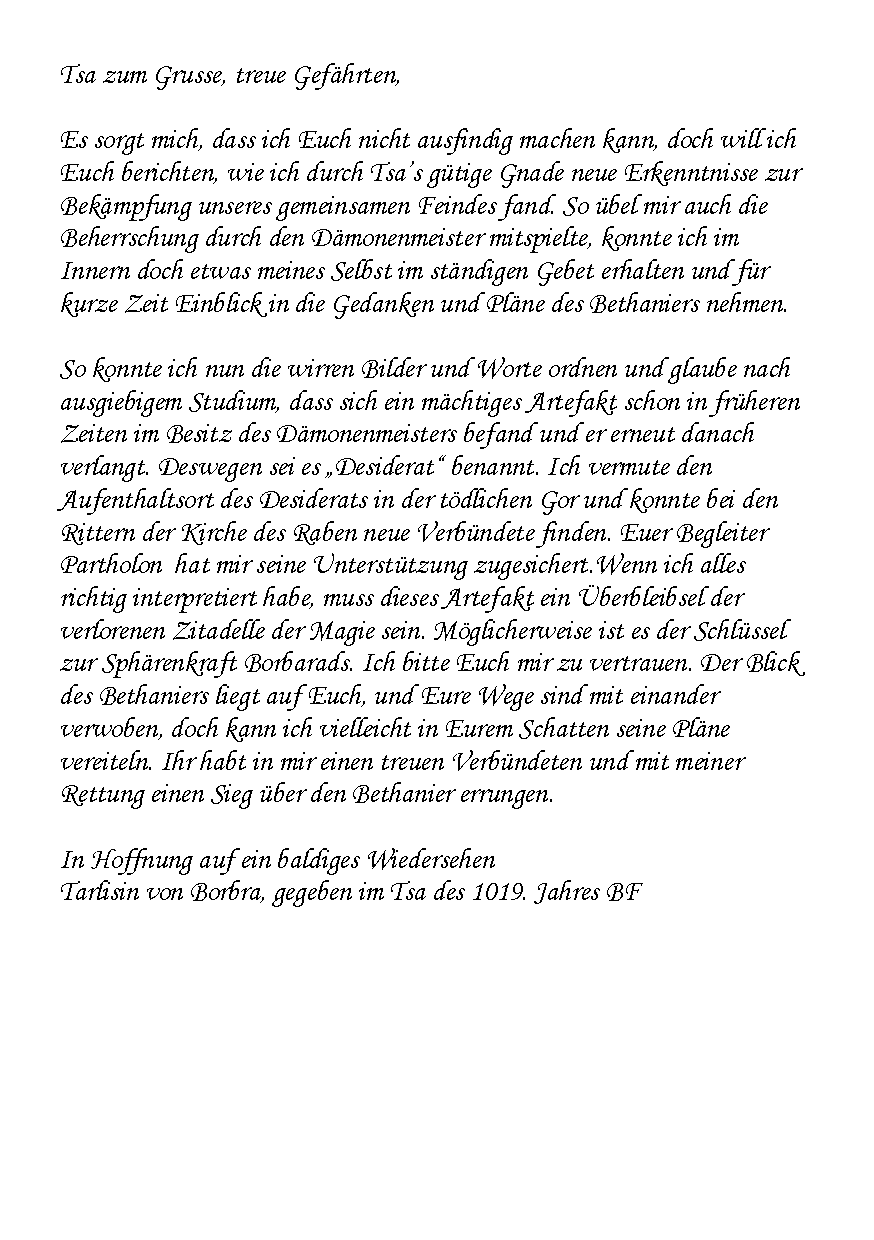
\includepdf[scale=0.9,pages=-]{handouts/part_3/gbabg_tarlisins_brief.pdf}

\includepdf[scale=0.9,pages=-]{handouts/part_3/Stahlburgurkunde.pdf}
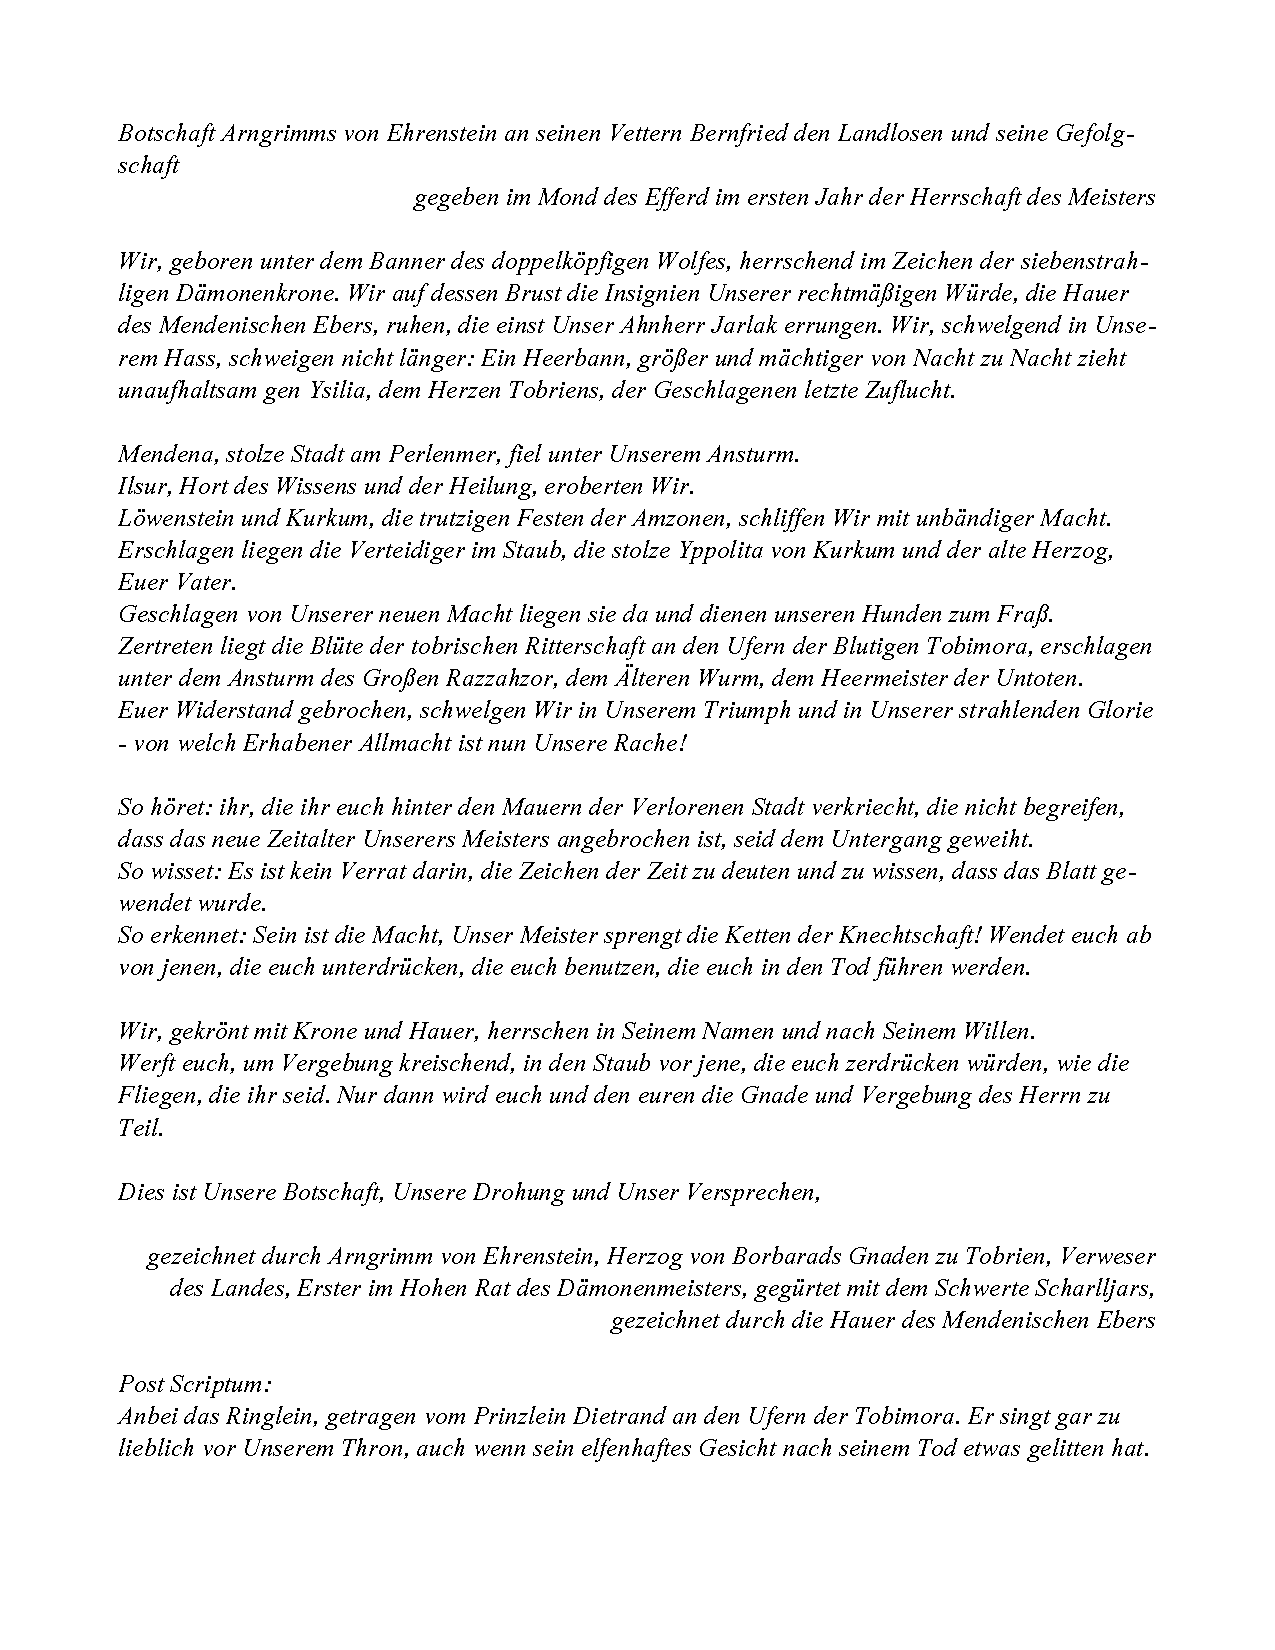
\includepdf[scale=0.9,pages=-]{handouts/part_3/wdw_botschaft_arngrimm.pdf}
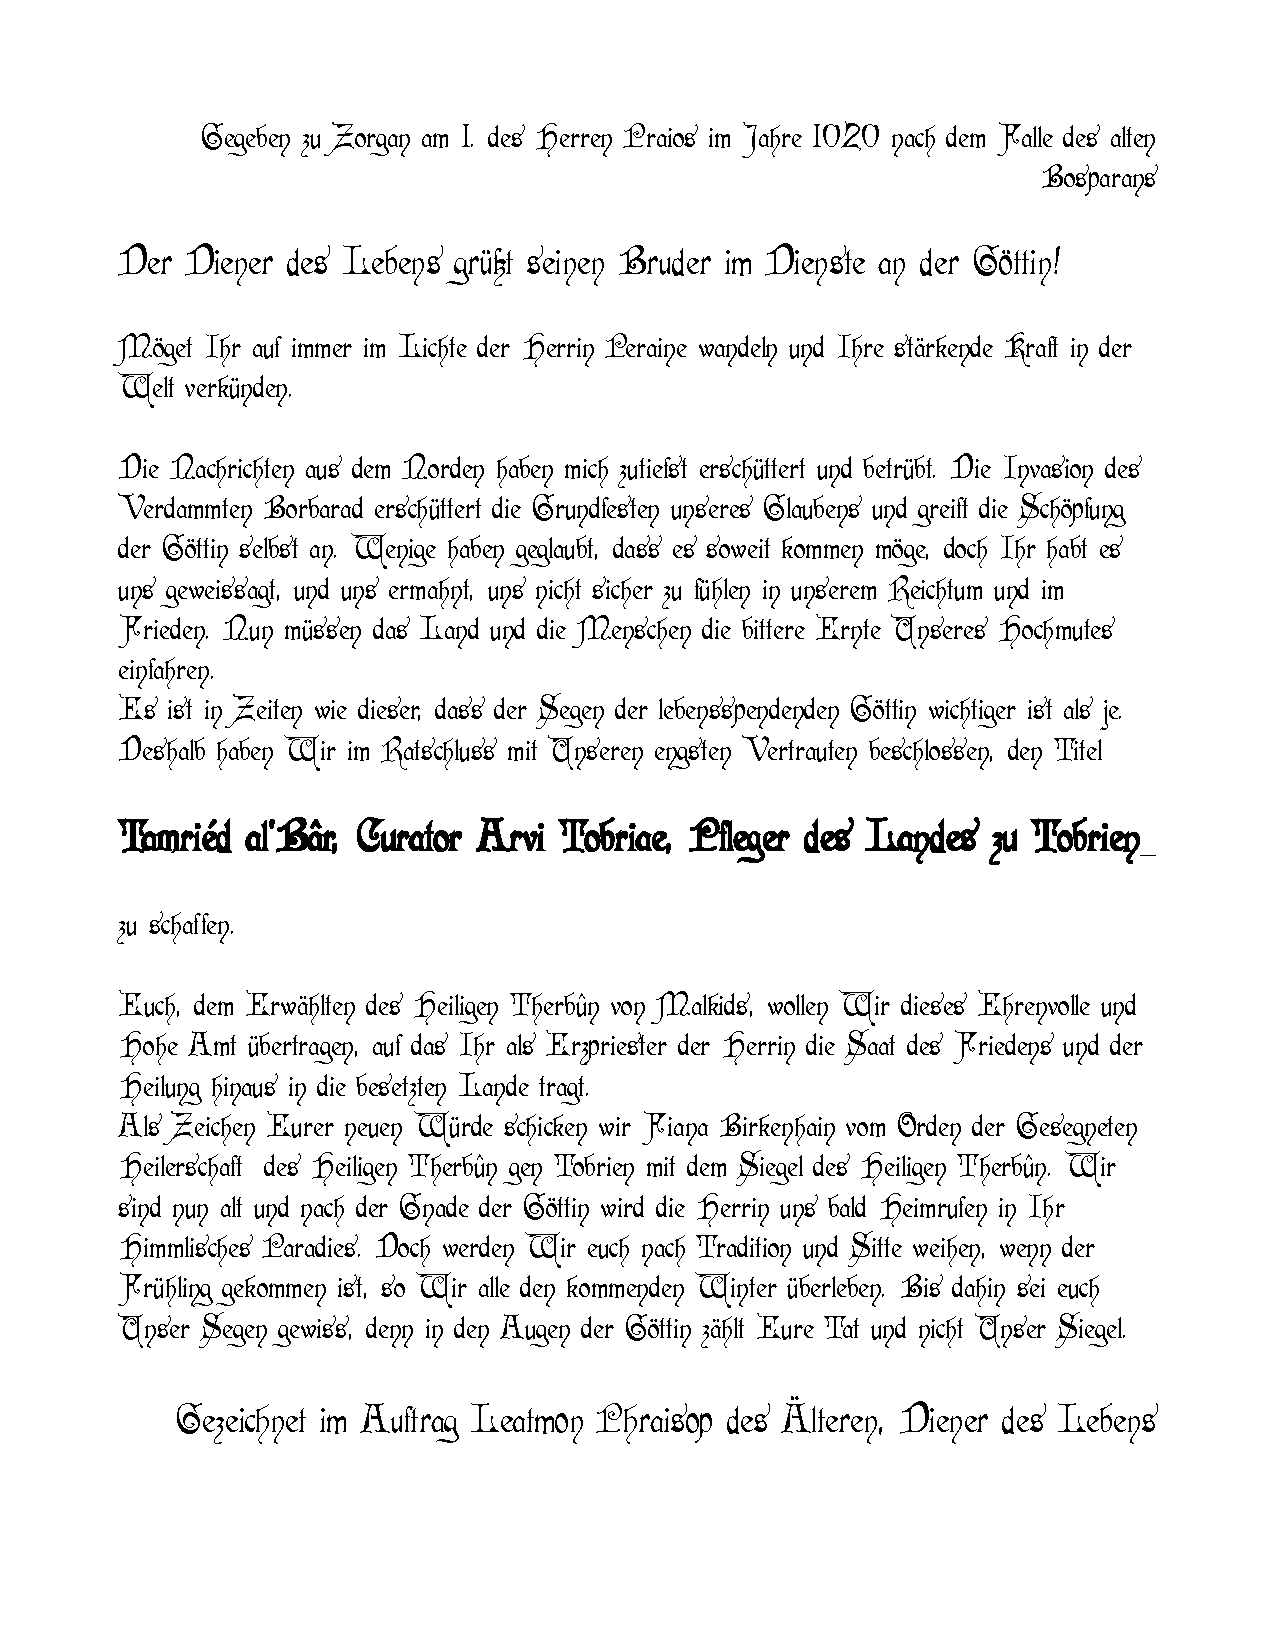
\includepdf[scale=0.9,pages=-]{handouts/part_3/wdw_brief_toran.pdf}
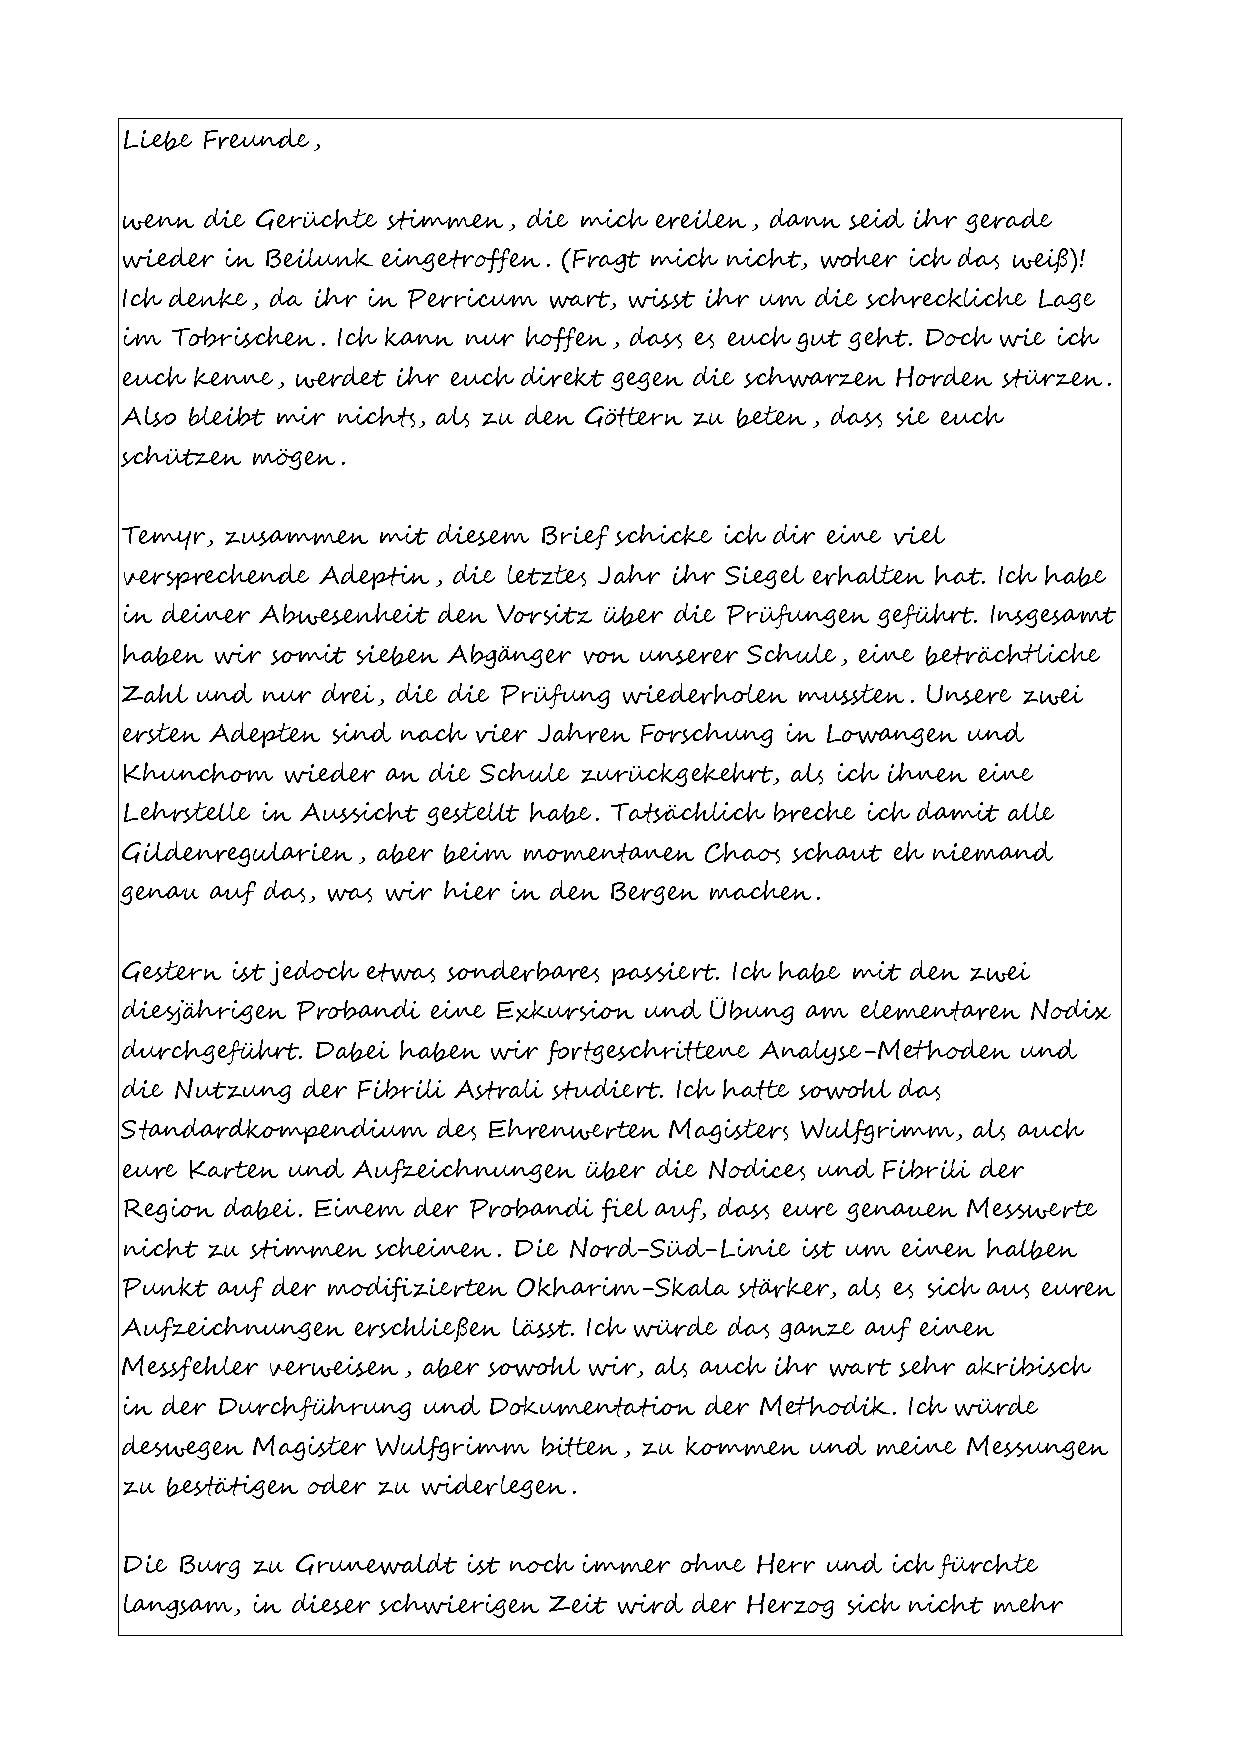
\includepdf[scale=0.9,pages=-]{handouts/part_3/wdw_brief_iliricon.pdf}

\part{Mächte des Schicksals}
\chapter{Euch zum Geleit}

Wir neigen uns dem Ende zu!
Im letzten Teil der Kampagne fehlen uns leider viele Abenteuer.
Das ist natürlich zum einen dem Studium geschuldet, und sicher auch dem Fakt dass niemand mehr großes Interesse daran hatte, nach dem Ende der Kampagne noch weiter zu schreiben.
Die AP hätte man ja gar nicht mehr ausgeben können!

Derrisch ist das hier nun die Darmstädter (und manchmal noch Kelkheimer) Zeit.
In Erinnerung geblieben ist mir natürlich als erstes unser monströser Tisch.
Ich glaube, nicht anderes hat mich in meinem Leben je so sehr den Respekt vor Handwerkern gelehrt wie dieses wackelige Konstrukt.
Über die Jahre hat er Kerzenreste, Pizzaflecken, und viele Erinnerungen aufgenommen, bis ich ihn (glaube ich ?) bei meinem Wegzug aus der Hoffmannstraße entsorgt habe.
Eine besserer Schriftsteller als ich würde hier jetzt noch eine große Lektion oder ein 


\chapter{Auf ein letztes Mal}

Lieber Waldemar,

Dieser letzte Teil der Geschichte wird wohl am kürzesten und fragmentiestark fragmentiert ausfallen. Von den Ereignissen auf der Queste nach den Sieben Kelchen, der Begegnung mit den Trollen, und der grausamen letzten Schlacht sind kaum noch Berichte zu finden.
Dennoch konnte Aria mir zumindest einen extrem detaillierten Bericht über die Schlacht auf den Vallusanischen Weiden zur Verfügung stellen, den Temyr verfasst hatte.
Auch wenn es vielleicht ein Vorurteil ist, aber ich denke, er beweist einmal wieder das Tulamiden unter all den vielen Völkern auf Deren die Wortgewandtesten sind.

Bitte füge die nächsten Zeilen nicht deinen eigenen Berichten zu, sondern verbrenne sie nachdem du diesen Brief erhalten hast. Ich muss dir von einer Geschichte erzählen, die vor einigen Wochen geschehen ist, aber niemand darf von ihr erfahren.

Seit Jahren hatte ich wenig von Temyrs Witwe Aria gehört. Die letzte Information, die ich hatte, war dass sie nach Khunchom gezogen war. Nach der Schlacht hatte sie wohl mehrere Jahre in Drakonia verbracht und bei den Elementarmeistern studiert. Aber nach diesem Exil hat sie eine Stelle an der Akademie in Khunchom angenommen, und ist wohl eine enge Vertraute der Akademieleiterin.

Ich hatte nur wenig Kontakt zu ihr, und sie war immer recht kalt in ihren Briefen. Ich hatte vermutet, dass ihr Schmerz um den Tod ihres Ehemannes einen Kontakt zu mir, oder zu anderen Gefährten aus der Zeit Klammsbrücks zu schmerzhaft für sie machte, und hielt es daher für höflich, nicht aufdringlich zu werden.
Aber mein Projekt, und das der Rhodensteiner, drang immer mehr in jene Zeit vor in der auch sie Teil der Geschichte wurde, und so beschloss ich im Zuge einer Studienreise einen Abstecher nach Khunchom zu machen. Ich wollte die Gelegenheit ergreifen in Temyrs Geburtsort ein paar Nachforschungen anzustellen. Im Zuge dessen erschien es mir angemessen, ihren Wohnort zu erfragen und sie um ein Gespräch zu bitten.

Doch dazu sollte es zuerst nicht kommen! Es war ein heißer Herbstabend, und ich hatte den gesamten Tag in der Akademie über Berichte über den Dämonenkrieg gebrühtet. Mein Tulamyd ist über die Jahre leider sehr rostig geworden, ohne Temyrs blumiges Fluchen in unseren Hallen, und so zog sich meine Arbeit bis zur späten Stunde hin. In der Art alter Menschen vergaß ich, dass es eigentlich zu spät für einen freundlichen Besuch war, und machte mich auf zu Arias Stadthaus.

Als ich auf die Tür zuging, fiel mein Blick durch ein Fenster. Ich weiß, es ist nicht die feine Horasische Art, aber die Neugierde war immer meine größte Sünde. Normalerweise würde ich einer alten Freundin auch nicht nach spionieren, aber was mich erblickte erstaunte mich so, dass ich nicht anders konnte als vorsichtig zu lauschen. Bitte verzeih mir dies!

In Arias Empfangszimmer saßen mehrere in lange, graue Reisemäntel gehüllte Gestalten. Elementarwesen servierten dampfende Getränke, doch das war nicht das auffälligste. Einer von ihnen saß so, dass ich sein Gesicht halb erblicken konnte, und das war es, was mich wie Rondras Donner traf: elfische Züge, die blasse Haut eines Nordmanns, und eine Augenklappe. Es war Firnen! Ich weiß, es ist unmöglich, aber ich schwöre dir, es war Meister Wulfgrimm. Seine Haut war dünn, fast schon Pergamentartig, und seine gesamte Gestalt hatte einen etherischen Character an sich, ich kann es nicht besser beschreiben.

Ich konnte nicht viel vernehmen, aber sie sprachen von Splittern und den Heptarchen! Mir wurde schnell bewusst dass ich nichts davon hören sollte, und ich schlich mich feige davon.

Als ich am nächsten Tag, zu angemessener Stunde, Arias Haus erneut aufsuchte, wurde ich freundlich, aber immer noch etwas kalt empfangen. Aria spielte eine perfekte Gastgeberin, lenkte aber von allen Fragen nach Firnen und Temyr geschickt ab. Ich denke auch um mich ruhig zu stellen gab sie mir den Bericht ihres Ehemannes von den Vallusanischen Weiden und schob mich mit diesem in den Händen fast schon zur Tür hinaus.

Ich werde weitere Nachforschungen antreten und dir als bald von ihnen berichten. Bis dahin überlasse ich dir das Ende meiner Arbeit hier, den finalen Abschnitt über das Wirken der Gezeichneten.

Dein alter Lehrmeister,\\
Iliricon Tannhaus

\chapter{Rohals Versprechen}

\section{Geleitwort}


\begin{flushright}
Claas Völcker, Toronto, den 28.05.2025
\end{flushright}


\section{Die Tagebücher}

\subsection{Der Auftakt des Conventes nach Firnen Wulfgrimm}
\paragraph{01. Ingrimm 1020 Bosparans Fall}
Heute zur Mittagsstunde haben ich und meine Freunde in der Yaquiertaler Hof Unterkunft bezogen. Abgesehen, von einem thorwalsschen Magus, der sich mit einem tulamidischem Magierer über den Preis, eines von dessen Seite aus unverkäuflichem nur wenig magischem Amulett stritt, verlief die Reise problem und ereignislos. Als Begleiter seiner Spektabilität iben Sahid haben wir den überzogensten Luxusflügel bekommen. Wir erwarten noch die Ankunft Torans in den nächsten Stunden, bis spätestens morgen, dann sind wir wieder alle vereint.

Es gild diesen Konvent ausreichend zu nutzen. Meine Verteidigung für die Verhandlung meiner Anklage sollte ich ausreichend untermauert haben bis dahin. Und viele Hypothesen habe ich in den letzten 3 Wochen ausgearbeitet, bezüglich unseres Feindes, und die werde ich nun, in Rücksprache mit den Forschergeistern, die die letzten 6 Jahre sicherlich so manches erdacht haben, zu bestätigen oder Verwerfen suchen.

Viel zu Denken gab mir vor allem das Gespräch mit Talesin von Borbra, den ich jüngst besuchte. Talesin war mit einer Expedition in die Gor aufgebrochen, und war nahe der schwarzen Festung vom untoten Drachen Razzzazor angegriffen worden.
Er meinte al Borbarad seinen Körper in Besitz genommen hatte habe er ein paar Gedanken des Sphärenschänders gesehen. Borbarad suche demnach nach einem irgendwie geartetem Desiderat, eim Schlüssel, der ihm die Sphären öffne. Und wie sich auch jetzt am Drachen zeigt, hat Borbarad trotz seiner Umtriebe im tobrischen immer noch starkes Interesse am alten Zentrum seiner Macht.

Wir unterhielten uns auch über die letzte Schlacht gegen den Bethanier, geführt von Rohal dem Weisen. Wir wälzten ein paar alte Schriften und fanden schließlich eine Abschrift, die den Bannfluch des Los zitierte. Seinerseits gesprochen von Rohal dem Weisen, verschwanden er und der Bethanier darauf hin aus der derischen Sphäre. Rohal riss demnach den Geiste Borbarads mit sich in eine Globule. Zeitlich und räumlich von Dere getrennt sollte niemals ein lebendes Geschöpf, den bösen Geist je wieder beschwören können. Zu blöd das es durch einen Toten geschehen konnte.

Zur borbaradschen Beherrschung bei der Verwendung borbaradianischer Canti ist wohl Cayonon Silberbraue zu befragen. Über die Globulenabschnitte unter Borbra sollte ich mich vielleicht einmal mit Aleya Ambaret unterhalten. Vielleicht schaffe ich es sogar heraus zu finden, wie der Dämon vor Ysilia meinen Schutzzauber umgehen konnte.
Heute Abend ist bereits erstes gemeinsames Bankett in der Akademie. Mal sehen, wen ich dort so antreffe.

Welch ein Disaster. Den Göttern sei Dank dass ich trotzdem jetzt hier sitzen und diese Zeilen schreiben kann.
Meine Reputation ist momentan nicht die Beste vor der weißen Gilde und auch die Graue schaut gespalten auf mich herab. Ich hate gerade erst problemlos alle Sicherheitskontrollen durchlaufen, als ein Rohalswächter auftauchte und behauptete ich sei bereits gekommen. In einm fast einstündigem Verhör unter allerlei magischen Überprüfungen konnt ich schließlich beweisen, das ich der Richtige bin, aber offensichtlich läuft auf dem Konvent ein Doppelgänger umher. Bzw. jetzt da er die Kontrollen passiert hat, ist er in wechselnder oder vielleicht sogar ursprünglicher Gestalt nicht mehr zu finden.

Mit Aleya Ambaret konnte ich bereits srechen und er meinte, dass die derische Sphäre um sich zu schützen. schadhafte Orte einfach abstoße. Als Globule in sich geschlossen liegen sie dort wo sie waren im Limbus verbannt. Wo sich heute das kleine Dorf Borbra befindet, erhob sich in früheren Zeiten, sowohl die Prachtvolle Residenz Assarabads, alsauch die Hallen des Tharsonius von Bethana, der sich Borbarad nennt. Offensichtlich hat Borbarad in früheren Zeiten ebenso an diesem Ort Sphärenrisse entstehen lassen um dämonischen Wessen Einzug zu ermöglichen.

Cayonon Silberbraue war leider nicht Anwesend, aber er hält morgen einen Vortrag, bei dem ich ihn eigendlich erwischen sollte.
Es war ein langer Tag und vor den Anstrengungen von mehreren Tagen Essens, unterbrochen durch mehrstündige Vorträge komplizierter wissenschaftlicher Sprechweise, mindestens in Bosparano gehalten, können wir alle eine gute mütze Schlaf durchaus vertragen.

\subsection{Der erste Vortrag nach Rezzanjin Al'Ahjan}

\paragraph{15.Ingerimm}
Da saßen wir also im großen Puniner Hörsaal als einige von vielen, denn der Hörsaal war bis zum Rand gefüllt und warteten erwartungsfroh auf den ersten Vortrag des Magierkonvents, welches an ebenjenem Tag begonnen hatte.

Doch dieser sollte auf sich warten lassen, da mehrere Weißmagier versuchten den vortragenden, Karjunon Silberbraue, ein anscheinend sehr umstrittener Magier vor allem bei der weißen Gilde, am Betreten des Hörsaals zu hindern. Es ging erst weiter als Firnen Nostrianus Eisenkolber, den Ordensanführer der Pfeile des Lichts mit seiner Anwesenheit ablenkte, sodass dieser seine ganze Wehemenz nicht mehr uneingeschränkt dem Verhindern der Vorlesung schenken konnte. Es ist ganz und gar nicht gut, dass der Kerl, der Firnen offensichtlich nicht leiden kann im Gericht über sein Wohl und Wehe entscheiden wird.

Als der Vortrag dann endlich begann, wurde schnell klar, dass ich unerwünscht bin, da der Vortrag auf Bosparano gehalten wurde. Ich ging also und beschloss den geheimnisvollen Treppenmord mal genauer zu untersuchen. Hierzu musste ich erst einmal herausfinden, ob der ermordete noch im Besitz des Amuletts war, um welches er mit den Thorwaller vor Punin gestritten hatte. Ich fragte also im Borontempel nach dem Verstorbenen Elenviner Magier. Diese hatten die Leiche tatsächlich aufgenommen, die weltlichen Besitztümer jedoch nicht bekommen. Also fragte ich bei Koosmar, dem Organisator des Konvents nach und tatsächlich hatte dieser die Gegenstände aufbewahrt. Da seine Assistentin, mit der ich sprechen konnte, aber nicht herausrücken wollte, ob das Amulett noch in seinem Besitz war, musste ich warten bis sich er selbst der Aufgabe annahm.

Da wir bis zur Mittagsstunden nichts mehr zu tun hatten, beschlossen wir unsere Zeit in der Teestube zu verbringen, wo wir auch Tarlisin von Borbra trafen, welcher gerade einer kleinen Truppe Schaulustiger von seinen Abenteuern berichtete. Anscheinend genervt von diesen übergab er uns die Aufgabe des Erzählers gewandt und machte sich aus dem Staub. Lang und breit erzählte ich daraufhin den versammelten Jungmagiern von den Abenteuern der Gezeichneten. Gegen Mittag wollte ich dann mit den anderen, die beim Vortrag zugehört hatten in der Stadt etwas essen gehen. Doch kaum waren wir auf dem Hof, schon hörten wir einen Schrei aus dem Garten. Schnell eilten wir zum Ort des Geschehens und fanden dort eine panische Elfe, sowie Elcarna von Hohenstein, der über den leblosen Körper eines horasischen Magiers gebeugt war. Neben diesem war ein Weinglas, der Inhalt zum größten Teil auf dem Boden verteilt und der Magier hatte keine sichtbaren Wunden. Man musste also davon ausgehen, dass der Wein vergiftet war. Schon kurze Zeit später kam auch Sirdon Koosmar angerannt und begutachtete den Toten. Ich fragte ihn nach dem Amulett des am Vortag verstorbenen Elenviner Magiers, doch er wusste noch von nichts. Wir überließen den toten Horasier den Magiern zum Untersuchen und gingen essen. Vor der nächsten Vorlesung ging ich nochmal zu Koosmars Assistentin und ließ mir erzählen, dass das Amulett nicht mehr im Besitz des Toten war. Das machte es umso dringlicher den Thorwaller aufzusuchen mit dem er gestritten hatte. Diesen fand ich zugleich in der nächsten Vorlesung und stellte ihn danach zur Rede. Nachdem ich Aleya Ambareth abgewimmelt hatte, der ihn begleitete, stellte ich den Thorwaller zur Rede. Es stellte sich heraus, dass er wohl nichts mit dem Mord zu tun hatte. Darüber hinweg wollte er auch nicht herausrücken, wieso er die Amulette brauchte, da er sie für seine Spektabilität Cellyana von Kunchom sammelte. Darüber hinaus gab er mir zu verstehen, dass diese einen Vortrag über ebenjenes Thema halten würde. Wieder waren wir nicht weiter gekommen. Aber es blieb uns wenig Zeit darüber zu grübeln, da wir uns für den am Abend stattfindenden Ball fertig machen mussten. Er war ein lustiger Abend, wir trafen viele bekannte Leute und feuerten ausgelassen. Doch gegen Mitternacht verschwand Temyr auf einmal und ward bis zum nächsten Morgen nicht mehr gesehen\dots

\subsection{Firnens Urteil nach Irian von Rabenmund}
\paragraph{16. INGERIMM im Jahr 5 nach Borbarads Erscheinen}
An diesem Nachmittag erfolgte die Analyse des Zweiten Zeichens, von der ich nur aus zweiter Hand berichten kann, da ich auf Grund meiner nicht zugehoerig zur magischen Zunft noch den gezeichneten ausgeschlossen war. So wurde anscheinend die Geschichte, wie Toran zu dem Zeichen kam und dessen Faehigkeiten, sowie die passenden Prophezeiungen besprochen.

\paragraph{17. INGERIMM}
Zur Morgenstund hoere ich mir den Vortrag zur Blutigen See an, waehrend die anderen im Vortrag zu den Untersuchungen ueber die Zerstoerung Altaias sitzen.

Am Vormittag finden die Analyse des Dritten Zeichens statt, an der aus oben genannten Gruenden auch nicht teilnehme.

Die wichtigsten Punkte waren, so wurde mir zumindest berichtet, Frage ueber einen Asfaloth-Pakt (Goetter und Daemonen, sind auch nur zwei Seiten derselben Medaille) durch Carolan Schlangenstab, ob es Einblicke in die echsische Kulur gaebe durch den Spinner Muntagonus, sowie Theamtisierung von Rezzanjin's Empathielosigkeit und der Verfolgung der Inkarnations-Theorie.

Gegen Mittag erhalten wir die Einladung zum Zwölfgötterjosten im Rondra in Perricum.

Zum Mittagessen werden wir von Rohezal vom Amboss in einer abgelegen Taverne eingeladen, der Firnen immer wieder besorgten Blicke zu wirft.

Als wir gerade wieder zur Akademie kommen, taucht plötzlich ein Karakilim über Punin auf und laesst den abgeschlagenen mit einer B-Zhayad-Rune gebranntmarkten Kopf von Atavar Friedenslicht fallen, aus dessen toten Mund die bedeutenden Worte kommen:

``Euer Zeitalter ist zu Ende, Kehrt zurueck ins Licht, Fabelwesen!''
Am Abend treffen wir auf Bitten Eternenwachts mit Rumina von Vinsalt und diskutieren mit ihr ueber die Moeglichkeit Borbarad als Sohn Nandus zu verdammen, da diese wehemmt dagegen ist, ein goettliches Wesen seine eigene Goettlichkeit abzuerkennen. Sie leidet gerade als Nandusgeweihte unter den taten den Nandussohns und hat eine Sinneskrise.
Bei unserer Rueckkehr wird Firnen beschuldigt den Magier Veranesco ermordet zu haben.

\paragraph{18. INGERIMM}
Am Morgen des 18. Ingerimms erleben wir, wie der Großmeister der Grauen Staebe, Tarlisin von Borbra, vom Hochmeister der Rohalswaechter Nostrianus Eisenkolber wegen Daemonenbuendelei angeklagt wird. Ein wahrhaft schwarzer Tag für die Einigkeit der Magier!

Wir wohnen Eternenwacht's Vortrag ueber die wachsende Borbarad und Daemonenverehrung in den gefallenen Landen bei, die sorgniserregend beobachtet wird, wozu aber noch keine Problembekaempfung gefunden wurde.
Am Ende des Vortrags erheben die Ucuriaten das Wort und verkuenden für die Welt, dass die Einigkeit der Kirchen für die Kampf wider dem gefallenen Alveraniar oberste Prioritaet hat, so nehmen die Ucuriaten nun Mitglieder aller Kirchen auf und wollen diesen als sacrosankte Botschafter dienen.

Am Nachmittag versammelt sich das Konvent, um über die Zusammensetzung von Rohals's Stein des Weisen zu entscheiden. Zur Dikussion steht, ob man die Onyx-Splitter wieder vereinen soll oder ob man auf Niobara's Warnung hoeren soll. Nach langen Ringen, gerade unter den Anhaengern von Rohals's Lehren, entschließt man sich den Stein des Weisen neu entstehen zu lassen.

Am diesen Abend finden wir uns ein,um dem Urteil ueber die Verfehlungen des Firnen Wulfgrimms zu lauschen.
Das Gericht setzt wie folgt zusammen:

Kläger: Spectabilitus Saldor Foslarin, vertreten durch Hauptfrau Lanzelind Heilenhorst, Pfeile des Lichts

Collegium Iustitium

Hohe Richterin: Spectabilita Racalla von Horsen-Rabemund, Convocata Secunda\\
Erster Gerichtsdiener: Spectabilitus Olorand von Gareth-Rothenfels zu Perricum\\
Zweiter Gerichtsdiener: Archomagus Rohezal vom Amboss\\
Erster Beisitzender: Spectabilitus Nostrianus Eisenkolber, Ordo Defensores Lecturia\\
Zweite Beisitzende: Spectabilita Prishya von Garlischgrötz, Convocata Prima der Grauen\\
Dritter Beisitzender: Archomagus Elcarna Erillion von Hohenstein zu Lowangen\\
Protokollant: Archomagus Carolan Schlangenstab zu Kuslik

Wächter des Argelionsrechts: Inquisitor Parinor von Oppstein\\
Weiser des Argelionsrechts: Magister Erechton, Sacer Ordo Draconis

Die Anklagepunkte lauten:

\begin{enumerate}
\item Besitz und Gebrauch verbotenen Schrifttums nach Codex Band V § 16.1
\item Täuschung der Obrigkeit durch Anwendung der Magie nach Codex Band V § 3.2
\item Kenntnis und Anwendung von untersagten Formeln und Canti nach Codex Band III § 14
\item Falschaussage vor einem Gildentribunal nach Codex Band V § 24.3
\item Flucht vor einem Gildentribunal nach Codex Band VI § 24.2
\item Heimtückischer Mord in zweifacher Ausführung durch Anwendung von Magie nach Codex Band V § 2.1
\item \begin{enumerate}
\item Der Mord an Wachmann Ernst Travian Rondratreu, Stadtwache zu Ysilia
\item Der Mord an Magister Minorum Dexter Hufstädter, Agent der Pfeile des Lichtes
\end{enumerate}
\item Paktierei mit dem Allerunheiligsten Herren der Rache in willentlicher Verleumdung der Zwölfgötter und aus niedersten Beweggründen Codex Band I § 14.1
\item Entzug als angeklagter Seelenpaktierer aus der Gerichtsbarkeit der Gilden durch den unter 6.1 genannten Mord nach Codex Band V § 2.3
\end{enumerate}


Im ersten Punkt kommt es zu einem Freispruch aufgrund eines Formfehlers der Anklage, er muss aber ein Bußgeld von 10 Dukaten bezahlen.

Unter Punkt 2 wird Firnen im Punkto: Anmaßung eines anderes Standes, als nicht schuldig angesehen, aber schuldig gesprochen für die Aneignung von mittelreichischem Staatseigentum, was an ein weltliches Gericht verwiesen wird.

Firnen gibt die Kenntnis von Tempus Stasis und Verbotenen Pforten zu und muss deshalb 10 Dukaten Bußgeld zahlen. Die Anklage zur Beherrschung der Blutmagie und der heptasphaerischen Invocation wird allerdings zurück gezogen.

Punkt 4 wird von der Anklage zurückgezogen.

Bei Punkt 5 müssen die besondern Umstaende beachtet werden unter denen sich Firnen für schuldig erklaert.

Bei beiden Morden wird Firnen wegen Mangel an Beweisen fuer unschuldig gehalten. Ihm wird aber vertretbarer Totschlag vorgehalten und er hat schon wieder ein Bußgeld von 10 Dukaten zu zahlen.

Firnen leugnet den Daemonenpakt nicht, haelt aber seinen Kampf gegen Borbarad und Seine Schergen dagegen.

Schlußendlich wird der Magier Firnen Wulfgrimm als schuldig in den Hauptanklagepunkt gesehen. Er wird aber aufgrund seiner Verdienste wider dem Nanduszwilling nicht der Purgation unterzogen, sonder aus der Großen Grauen Gilde des Geistes verbannt.

\subsection{Das Auffinden des Mörders nach Temyr ibn Sahid}

\paragraph{19. Ingerimm im Jahre 1020 nach dem Falle Bosparans}
Am nächsten Morgen begaben wir uns direkt nach dem Frühstück in die Hallen der Akademie zurück, um dem traditionellen Götterdienst oder der Konkurrenzveranstaltung des Tomeg Aterion -- ``Warum wir nicht im Götterdienst sind'' -- beizuwohnen. Die Inhalte der letzteren lassen sich freilich in einem äußerst populären tulamidischen Sprichwort zusammenfassen, dessen Erklärung hier aber zu weit gehen und die leutseligen Gemüter meiner Gefährten unnötig belasten würde\dots Kaum hatten wir uns jedoch hernach wieder zusammengefunden, als Sidor Kosmaar mit ahnungsvollen Schritten herangeeilt kam und unsere Sorgenliste um einen weiteren Punkt ergänzte. Der Mörder, dessen verachtenswertes Geschick schon die letzten Tage den Konvent in Atem gehalten, hatte ein weiteres Opfer gefordert: eine junge Magistra namens Yaneska Yanolof, die auf dem Weg zu ihrer Herberge erdrosselt aufgefunden worden war.

Was war das Ziel des Attentäters? Wie stand er in Verbindung mit den Plänen des Thorwaler Magus und seiner Vorgesetzten, Seliana von Khunchom, in welche Rezzanjin Einblick zu gewinnen versucht hatte? Und war es eben dieser, der bereits am ersten Tage in Gestalt Firnens den Konvent aufgesucht hatte? Über all diese Fragen diskutierten wir reiflich und hitzig, und griffen dabei einen Gedanken auf, den Firnen als erster gefasst hatte, nämlich die Identität des Assassinen betreffend. Handelte es sich bei dem Schurken, der ja in der Kunst der Magie durchaus bewandert schien, um einen der abtrünnigen Tuzaker Magier, die so früh schon unsere Pläne gestört hatten? Wenn ja, so würde er mit Sicherheit auch hinter uns selbst her sein, und seiner Chance unter allen Umständen harren. Die Überlegung schien naheliegend, und so fassten wir den Plan, dem Täter eine falsche Fährte auszulegen und seiner in persona habhaft zu werden. Als Ausleger der Falle wählten wir meine feierliche Ernennung zum Erzmagus, der sich nach guter tulamidischer Tradition eine weniger offizielle, aber dafür weitaus ausschweifendere Festivität anschließen musste. Mit meinem Kopf in Reichweite, so folgerten wir, würde es dem Mörder eine unwiderstehliche Verlockung präsentieren, erneut zuzuschlagen. Nur dass in diesem Augenblick, selbstverständlich, wir selbst zuschlagen würden\dots

Wir besprachen den Plan in aller Eile, aber gebotener Vorsicht mit der Magistra Prima von Garlischgrötz, die unserem Vorhaben zustimmte und erste Vorbereitungen in die Wege leitete. Als wir uns zurück in das Gedränge des Konvents begaben erreichte uns eine Depesche des Hesindetempels, welche zur Audienz bei der ehrenwerten Haldana von Ilmenstein lud. Nach dem letzten Vortrag des Tages, in welchem Dscheleff in einer flammenden Rede den Zusammenhalt der Magierschaft beschwor und zur Unterstützung der Gezeichneten aufrief, verließen wir die Hallen der Akademie am Nachmittag und wandten unsere Schritte zum Haus der weisen Göttin. Die Magistra der Magister empfing uns freundlich und dankte für unsere Bemühungen im Kampf gegen Borbarad. Ebenso lag es ihr jedoch daran, Erkundigungen einzuziehen, worin wir ihr mittels eines ausführlichen Berichts aushelfen konnten. Über unser Auskünfte war es schon Abend geworden, und die Geweihte hieß uns zu bleiben für ein Treffen von Hesinde- und Magiergeweihten. Uns so trafen dann im Herzen der Nacht, zur Hesindestund, die Geweihten der Göttin ein, um die allgemeine Verdammung des Borbarad vor den Augen von Göttern und Menschen zu beschließen. Die höchsten Geweihten des Phex, des Nandus' und der Hesinde traten um den Altar, und mit donnernden Stimmen, die nicht Menschen, sondern Göttern gehörig waren, verkündeten sie das Wort vom einigen Ratschluss. Ein würdiges und gerechtes Zeichen im Angesicht eines Götter und Menschen verachtenden Gegners!

\paragraph{20. Ingerimm}
Der folgende Tag begann mit einer gewaltigen Überraschung, der sich noch weitere anschließen sollten -- gute wie schlechte. Als wir nämlich wie üblich unsere Schritte zum Pentagrammaton lenkten, versperrten uns dort die Rohalswächter unter Nostriamus Eisenkolber den Weg. Selbiger trat mit gequälter Miene vor und übergab Toran mit zitternden Händen seinen Onyxstab, den er zuvor unter keinen Umständen herzugeben bereit war. So erstaunt waren wir über dieses kleine Wunder, dass wir kein Wort hervor brachten -- im Gegensatz zu Eisenkolber, der uns mürrisch beschimpfte und auch sonst wieder ganz der Alte zu sein schien. Mit diesem Schatz in den Händen begaben wir uns ohne Umschweife zu Seliana von Khunchom, die über alle Maße erfreut über einen Stein dieser Größe war. Danach widmeten wir uns weiterhin der Vorbereitung unserer Falle, bis die ersten Vorträge des Abends unsere Aufmerksamkeit verlangten. Abermals teilten wir uns unserer Interessen gemäß auf und besetzten verschiedene Hörsäle, um das Angebot des Konventsplans auszuschöpfen. Der Vortrag des Khadil Okharim beleuchtete die Fortschritte bei der Erstellung des bastrabunschen Bannschildes, an welchem wir selbst tatkräftig mitgewirkt hatten. Die Rekonstruktion der Bannformeln schien gut voranzugehen, doch hatten sich tiefere Probleme bei der Entschlüsselung der materiellen Komponenten der Spruchform aufgetan. Magister Okharim war gerade dabei, die feineren Züge seiner Analysen zu erläutern, als auf dem Flure ein unglaublicher Tumult ausbrach und die versammelte Magierschaft in heilloses Durcheinander stürzte: Während des parallelen Vortrages der Magistra von Garlischgrötz hatte sich, wie Firnen später atemlos berichtete, ein Riss im Sphärengefüge aufgetan, aus welchem sich unaufhörlich Zantim ergossen und die Zuhörer angegriffen hätten. Irgendwie gelang es zwar, den Dämonen Herr zu werden, aber unter welchen Verlusten! Viele hatte die Dämonenbrut hingemetztelt oder schwer verletzt; das eigentliche Unglück wurde aber erst später offenbar. Im Schutze der Verwirrung und Panik waren nämlich die gesammelten Onyxsplitter aus den Räumen der Seliana von Khunchom entwendet worden, nicht ohne ihrem treuen Untergebenen Ilachim die Kehle durchzuschneiden.

Nun hieß es, auf das Gelingen unserer Falle zu bauen und den Mörder, wenigstens jedoch die Steine, zurückzubringen. Nachdem der feucht-fröhliche Abend im besten Gasthaus Punins ausgeklungen war, begab ich mich allein durch die nächtliche Gassen der Stadt zurück zu unserer Unterkunft -- stets gedeckt von den unsichtbaren Schatten meiner Freunde, die mir unauffällig folgten. Und tatsächlich dauerte es gar nicht lange, bis sich der Unhold aus seinem Versteck begab. ``Paralysis!'' hörte ich hinter mir eine Stimme schreien und eine Welle magischer Energie brandete über mich hinweg. Da ich aber mit einem solchen Zug gerechnet hatte, gelang es mir den Zauber abzuschütteln und dem Magus -- es handelte sich tatsächlich um einen Maraskaner -- einen saftigen Ignifaxius entgegen zu schleudern. Sogleich sprangen meine Gefährten hervor und warfen sich in das Kampfgetümmel. Der Magier hatte mit so viel Gegenwehr freilich nicht gerechnet und versuchte sofort, dem Kampf zu entgehen: Sein ganzer Körper schien in sich zusammenzufallen, zu schrumpfen, da wuchsen schwarz-ledrige Schwingen daraus und mit raschem Flügelschlag verschwand der Blutsauger in der Nacht. Rezzanjin jedoch rannte, von der Kraft eines Zaubers erfüllt, hintendrein, und konnte den Maraskaner bis zu einem verfallenen Turm verfolgen, in dessen labyrinthischen Eingeweiden er den Kerl aber verlor. Als der Rest von uns endlich mit menschlicher Geschwindigkeit dort eintraf, hatte Rezzanjin bereits das ganze Versteck auf den Kopf gestellt und neben den Steinen auch einen Brief entdeckt, der an einen gewissen Torben Dergeler adressiert und von unserer alten ``Freundin'' Azariel Scharlachkraut unterschrieben war. Offfenbar hatte sich die Hexe noch bis gestern selbst in Punin aufgehalten und hatte das Wirken des Tuzakers überwacht. Weiterhin enthielt das Schreiben Anweisung, eine gewisse Hexe aus Maraskan namens Lavinia aufzusuchen, sobald der Auftrag erledigt wäre. Wenigstens dem hatten wir einen Stich versetzen können. Mit den Steinen im Gepäck begaben wir uns zur Akademie.

\paragraph{21. Ingerimm}
Das Arbeitskabinett der Convocata Prima war schon bis auf den letzten Platz ausgefüllt, als wir tags darauf auf dem Konvent eintrafen. Seliana von Khunchom hatte bereits die Fakten rund um die Onyxsteine und ihre Arbeit resümiert, und erging sich dann in weiteren Ausführungen über die nun zu beschließende Vorgehensweise. Zunächst einmal galt es, für den Stein der Weisen die fähigsten Artefaktmagier, Analysten und Handwerker auszuwählen, die diesem delikaten Gegenstand Form verleihen sollten. Die anwesenden Magier diskutierten wohl manche lange Stunde, bis endlich die fünf Betreffenden zusammengestellt waren. Der Ratschluss lautete auf: Salpicon Savertin, Firnen Wulffgrimm, Salandrion Farnion Finkenfarn, Ragnos vom Svelltal und mich, Temyr ibn Sahid. Das Wunder konnte vollzogen werden.

\subsection{Der Stein der Weisen nach Firnen Wulfgrimm}

\paragraph{21 Ingrimm 1020 Bosparans Fall}
Der Stein des Weisen soll nun beschlossener Maßen wieder zusammen gesetzt werden. Sowohl Temyr als fähiger Artefaktmagierer, als auch ich, mit meinen überdurchschnittlichen Analysefähigkeiten, werden dabei mithelfen dürfen. Da Temyr sich bereits ein paar Gedanken machen wollte, über eine mögliche Artefakt Thesis, zur Reaktivierung der vorhandenen Strukturen, analysierten wir noch einmal einen Großteil, der Splitter. Dabei erregte Zulhamid in mir einen schrecklichen Verdacht. Ich wollte soeben einen Analys zaubern, da offenbarte mir der Magiermogul bereits den gewünschten Anblick. Er war völlig aus dem Häuschen und wollte keine Sekunde länger mit dem Zusammensetzen warten. Die magischen Strukturen trügen SEINE Signatur, die Art und Weise, des Assarabat, beziehungsweise des Bethaniers, und das Artefakt brächte uns einen Weg IHN zu finden. Was ist nun, wenn wir weder Kontakt zu Rohal erreichen, noch ihn beschwören können, sondern den Bethanier rufen? Ich vermag mir dieses Schreckensszenario kaum auszumalen. Das Artefakt ist unsere einzige Handlungsmöglichkeit und ich bete zu den Göttern, dass sie uns etwas Gutes bringt.

Toran kam kaum später herein. Er hatte im Tempel meditiert und eine beunruhigende Ahnung hatte ihn erreicht. In Gedanken an die Göttin, sah er einen Turm wie aus Glas und goldene Schuppen, und ein ungutes Gefühl beschlich ihn, dass ihn jetzt noch frösteln lässt, wenn er daran zurückdenkt. Der einzige unsichtbare Turm, er wird eigentlich nur durchscheinend, den ich kenne, ist der Hofmagierturm im Ambossgebirge. Derzeitig verwahrt und bewohnt von Rohezaal vom Amboss.

Wir wollten Rohezaal von unseren Theorien und Befürchtungen in Kenntnis setzen, doch er bat uns ihn erst am frühen Abend in der kleinen Bibliothek zu treffen. Torans Vision könnte eine seiner Theorien bestätigen.

Rezzanjinn beschloss uns zur Unterredung zu begleiten, Irian hatte schon am Mittag die Stadt verlassen, warum wusste keiner. Tatsächlich erwartete uns Rohezaal bereits in der kleine Bibliothek. Er hob gerade zu sprechen an, uns eine Mitteilung immenser Bedeutung machen zu müssen, als er nach vorne sackte. Ein kleiner Borndorn ragte aus seinem Nacken. Während Toran, Temyr und ich uns erfolgreich bemühten den Erzmagier im Leben zu halten, bemühte sich Rezzanjinn den bereits bekannten Maraskaner, der hinter einem Vorhang verborgen gestanden hatte, dingfest zu machen. Trotz eines abgeschlagenen Armes, entkam der Asfalothpaktierer als Vogel durch das Fenster. der Arm wuchs nach. Rohezaal erklärte uns von einem Hexagramm aus Orten, die mit Rohals Wirken zu tun gehabt haben. In der Mitte des Hexagramms der Ort Wagenhalt, in dem Rohezaal der Legende nach erschien. Rohezaal glaubte, das der weise Magier im Falle einer Beschwörung, über diese Orte seinen Weg gehen würde von einer geistigen Gegenwart, bis zur Verkörperung. Sobald sich die Theorie bestätigen würde, wolle er in den Amboss reisen, und versuchen, eine Verkörperung zu verhindern, den usn allen klingt noch immer die Warnung Nihobaras von Anchopal in den Ohren: "Niemals vollendet sei der Ruf nach den Beiden, um göttliche Allmacht auf Deren zu meiden." Der Plan Rohezaals klingt verrückt, aber er könnte klappen.

Eine geraume Zeit schon von unseren Stäben, durch ihre Zerstörung entbunden, beschlossen Temyr und ich ihre Spektabilität zu Punin zu bitten, uns Material aus den Akademiegewölben nehmen zu dürfen, um uns neue Stäbe zu erschaffen. Die Bitte schlug sie uns nicht ab, und nun wird sich zeigen, ob wir in einer Nacht zu vollbringen vermögen, zu dem der Eleve knapp eine Woche benötigt.

Ich fand einen knorrigen Stab von etwa eineinhalb Schritt Länge, aus dem Holz der Steineiche, das ich nicht im Besitz einer Punier Akademie vermutet hätte. Vielleicht war es ein Experiment gewesen, das die Akademie einst beschlagnahmt hatte, denn es befand sich in die Verästelung am oberen Ende des Stabes geschnitzt, eine ebenso ungewöhnliche Walrune, wie bei den Thorwalern üblich. Die Verästelung beinhaltete bereits eine Fassung, nur der Stein schien abhanden gekommen zu sein. Ich fand passend einen bordeaux farbenen grobbehauenen Topas, den eine Silberne Mondsichel zierte.

Das Holz scheint eine ungewöhnlich große Affinität zu Blitzen und Feuer zu haben. Der Stein hat eine eigene antimagische Kraft. Die Walrune hat sich magisch mit der silbernen Mondsichel verbunden. Es muss eine Art thorwalsches Zauberzeichen sein, es wirkt der Verständigung zugehörig. Kaum hatte ich den Stein in den Stab eingesetzt, erschienen magische Zeichen, des Feuers und der Antimagie in silbrigem Arkanum, und ebenso Flammen die, sich um den Stab rankend, diesen schmücken in unvergleichlicher Weise. Ich denke der Stab ist passend wie kein zweiter. Und ich danke den Götter für die merkwürdige Vielfalt der Sammlung einer so alten Akademie wie der in Punin.

Etwa zwei Stunden vorm Weckruf der Kirchenglocken traf ich Temyr in der großen Halle der Akademie. Er war ebenso fertig geworden. Es war ihm gelungen einen etwa zwei Schritt langen Stab aus Rashtulszeder zu bergen. Nun schmückte ihn zu dem ein Amethyst in Form einer stilisierten Rose.

Müde und zufrieden kehrten wir in unser Gasthaus zurück. Wenigstens die letzte Stunde werde ich noch zu schlafen versuchen, bevor vielleicht der Größte Tag seit langer Zeit anbricht.

\paragraph{22. Ingrimm 1020 Bosparans Fall}
Es bereits Abend ich bin gleichermaßen erschöpft und verstört. Die Ereignisse des Tages übertreffen fast alles bisher erlebt an Unvorstellbarkeit. Doch bei allem Schrecken bleibt ein Schimmer der Hoffnung.

Also von Vorn: Wir begannen bereits zu früher Stunde mit der Rekonstruktion des Steins des Weisen. Die bereits angefertigten detaillierten Analysen erleichterten das Vorankommen erheblich. Stück für Stück setzte sich das Artefakt zusammen, und obgleich es ungemein Kräfte zehrend war, dauerte es nur wenig Stunden. Das ungeheuerlichste Artefakt, das ich je gesehen hatte war zusammen gesetzt worden. Ein Schwarzes Auge, in Form einer etwa Kopfgroßen Kugel, das nicht die Zeit, sondern die Spähren zu durchblicken scheint, und eine Invokation herbeiführen konnte die nicht der siebten Sphäre zugeordnet werden kann.

Die drei Konvokati Primae der Gilden legten ihre Hände an das Artefakt und schienen in Trance zu versinken. Bilder zogen durch den Raum, Bilder jener Orte, die Rohezaal dem Hexagramm zugeordnet hatte. Er schien also in seinen ersten Punkten Recht zu behalten. Er bat uns ihn zu seinem Turm zu begleiten, und mit ihm flogen wir auf seinem Freund, Faldegorn, einem Kaiserdrachen, ins Ambossgebirge.

Tatsächlich offenbarte sich uns dort das gelegentliche aber seltene Spektakel, den unsichtbaren Turm zu sehen, in der durchscheinenden spiegelnden Art, die ihm im Volksmund diesen Namen einbrachte. Rohezaals Tochter eilte uns entgegen. Sie sagte alle Tiere habe die Gegend verlassen, beziehungsweise, haben sich auf einer Bergwiese, ein Stück unterhalb des Turmes gelegen, versammelt. Auch wir eilten schnellen Schrittes zu dieser Wiese und tatsächlich: Als wir dort ankamen bot sich uns ein Anblick, den ich auf immer in meinem Herzen tragen werde. Aus den leichten Schwaden eines Bergnebelfeldes heraus kam ein Mann geschritten. Seine Haltung edel, sein Gang bewusst und rechtschaffend, sein Blick voller Güte und seine Worte voll Weisheit. Sein Wesen voller Freundlichkeit. Rohal war zurückgekehrt. Als wir mit seiner Hilfe unsere Sprache wieder fanden, bedrängten wir ihn schließlich doch mit den dringlichsten Fragen, die uns seit geraumer Zeit nun schon, so arg beschäftigten. Was sollten wir unternehmen um Borbarad aufzuhalten? Rohal sah uns unsere Zielstrebigkeit nach, auch wenn er uns ermahnte stets auch die Welt im Auge zu behalten, wenn wir unseren Weg zu sehen versuchen. Er verriet uns die Schwachstelle Borbarads: Der Bethanier hat Satinav um seine Zeit gebracht, als er sich zurück holen ließ, und mehr denn je hat er seine Zeit verkauft. Wenn wir den Bethanier nun zu hindern gedächten, so sollten wir seine Zeit finden und hüten. Diese Aufgabe übertrug er uns und im besonderen Temyr, dem er zum Zeichen seines Auftrages, die Kappe des Weisen auf sein Haupt setzte. Der fünfte Gezeichnete ist erschienen. Er trägt das Zeichen der stählernen Stirn und das Wissen um seinen Frevel.

So erleichtert über die Einsicht in die Tiefen der Welt und die begründete Hoffnung auf ein Morgen, standen wir ahnungslos auf der Bergwiese und redeten noch von Angesicht zu Angesicht mit dem Weisen persönlich, als das Unheil heraufzog. Der Himmel verfinstert sich und die Vögel hatten längst das Weite gesucht, als sich die Sphären öffneten und Borbarad hervor trat. Auf seinem Haupt trug er, und noch jetzt schaudert mich die bloße Erinnerung dieses Anblicks, die siebenstrahlige Dämonenkrone. Sieben Erzdämonen hatte er seine Seele versprochen in der Gewissheit, dass sie sie nie würden fordern können. Sie sollten sich selber gegenseitig zerfleischen, um den größten Schatz der Niederhöllen, seit der Versuchung des Namenlosen, die Seele des Alveraniers des verbotenen Wissens.

Borbarad lachte Rohal aus, ob der Schwäche ihn nicht vernichtet zu haben, er beschämte die Liebe die ihm der weise Zwillingsbruder entgegenbrachte, überhörte die Warnungen und den Rat. Er lästerte seines Unvermögens auf die Hilfe des Los angewiesen zu sein, und sprach den ebenso schrecklichen wie verächtlich kurzen "Bannspruch des Borbarad": "Rohal sei nicht mehr!" wir wollten fliehen, wie Rohal uns als letzte Worte riet, doch der Bethanier hielt die Zeit, und ließ sie nach seinem Willen fließen. Wir mussten mit ansehen, wie Rohal langsam verblasste, bis er schließlich verschwand. Unsere Freiheit erlangten wir erst wieder, als Borbarad sich abwendete. "Zerreißt sie!", sprach er und überließ einem Dutzend Zants das Feld. Wir kämpften einen ungleichen Kampf. Ich sah noch wie Irian von zwei Zants in die Zange genommen, ein Bein ausgerissen wurde, als mir selbst, durch die erlittenen Wunden die Sinne schwanden. Rezzanjinn hat sich gut geschlagen, und Temyr hatte, Phex muss ihm geholfen haben, kaum ein Kratzer abbekommen. Toran muss beinahe mit seinem Leben für unser Überleben bezahlt haben, doch die Göttin gewährte ihm ihre Gunst. Und ohne die Unterstützung Rohezaals, und vor allem Faldegorns, hätte wahrscheinlich keiner von uns diesen Massaker überlebt, aber Borbarad hatte uns unterschätzt, unser Freunde die uns helfen, und die Götter die uns schützen.

Er hat uns den Weisen Anführer genommen, doch die Saat war längst gelegt. Der Auftrag längst erteilt, sein Zeichen längst gegeben. Auf dass er verschwinden musste, nicht aber konnte genommen werden, jenen die nun nach seinem Rate handeln.

\subsection{Borbarads Zeit rekonstruiert durch Iliricon}

{\itshape

}
\todo[inline]{Fragment}

\subsection{Die Reise nach Drakonia nach Rezzanjin al'Ahjan}

\paragraph{Mitte Rahja}
Nach dem Zwischenfall in dem kleinen beschaulichen Jassafheim, bei dem Irian fast umgekommen wäre setzten wir unsere Reise fort. Entgegen unserer Erwartungen und zu unserer Freude ließen sich unsere Verfolger vorerst nicht mehr blicken. Keine lächerlichen Hinterhalte und auch keine als Dorffrauen verkleideten Hexen, die versuchten uns umzubringen. Wir hatten also ein paar schöne Tage, in der ich die Schönheit des Yaquirtals im Sommer genießen konnte.

Am frühen Nachmittag dann kamen wir in Tenn an, einem beschaulichen Dorf an der Mündung des Bosquirs in den Yaquir. Eigentlich mussten wir hier, laut Arya, ab, um den Bosquir bis zur Quelle zu folgen, um von dort aus in Hochgebirge vorzustoßen. Doch vorher wollten wir noch Ausrüstung besorgen, um in den auch im Sommer schneebedeckten Bergen des Raschtulswalls nicht zu erfrieren. Wir beschlossen nach kurzer Diskussion, dass diese in Punin wohl am besten zu holen sein würde, weshalb wir den halbtägigen Eilritt zu unserer Villa vor Punin auf uns nahmen. Unser Hausverwalter war ziemlich überrascht, als wir am späten Abend in der Villa ankamen. Doch schon am nächsten Morgen brachen wir nach Punin auf. Es dauerte eine ganze Weile, bis wir die Winterkleidung zusammenhatten, im Sommer ist sie nur schwer zu bekommen, und noch eine ganze Weile länger, bis Temyr von seinem eigenen kleinen Einkaufsrundgang zurück war. Danach machten brachen wir wieder auf und erreichten am früher Abend, gerade noch rechtzeitig für die Feierlichkeiten anlässlich des Rahjamondes, das kleine Örtchen Schlangentod. 

Nachdem wir uns im örtlichen Gasthaus einquartiert hatten, mischten wir uns, bis auf Irian und Ragnos unter die Feiernden. Doch plötzlich, die Praiosscheibe war noch nicht hinter dem Horizont versunken, schoss ein Feuerpfeil über die angrenzenden Häuser und schlug in das große Festzelt ein, welches sofort Feuer fing. In dem nun ausbrechenden Tumult hörte ich Ragnos auf einem Dach noch schreiend auf Angreifer aus dem Wald hindeutend, bevor er von seinem Dach verschwand und ich, mein Tuzakmesser ziehend, in Richtung Wald lief. Dort sah ich Ragnos, vermutlich einem Pfeil ausweichend hinter einem Baum verschwinden und einen bulligen Mann mit einem Tuzakmesser in der Hand auf mich zu rennen. Schnell entwickelte sich ein Kampf, in dem ich plötzlich mit fürchterlichen Schmerzen flachlag, als der Bruderlose vor mir mich berührte. Den Treffer, den er landete, heilte Toran, der wohl auch gekommen war. Doch kaum hatte ich mich erholt, waren auch schon fast alle Gegner wieder verschwunden. Nur Firnen hatte mit der Hilfe von Temyr einen Zwerg erledigt, der, wie Firnen erklärte, wohl mit dem Praios entgegenstehenden Erzdämonen ein Pakt geschlossen hatte und sich deshalb Firnen entledigen wollte. Irian war mal wieder, wie immer, von Travian von Rabenmund mit einem Schlag erledigt worden, während Ragnos irgendwie drei Gegner beschäftigt hatte, ohne mehr als ein paar Kratzer einzustecken. Insgesamt konnten wir sechs Gegner ausmachen. Travian von Rabenmund, der Kerl mit dem Tuzakmesser, Savolina die Hexe, mit der Temyr schon in Grunewaldteine Auseinandersetzung hatte, eine brabaker Magierin, eine weitere Hexe und der nun tote Zwerg. Hierzu würde wohl noch Torben Dergeler hinzukommen, der im Kampf, wohl aufgrund seiner hierbei unzureichenden Fähigkeiten keine Erscheinung gemacht hat, aber uns schon zuvor angegriffen hatte.

In der Nacht erholten wir uns von unseren Verletzungen, immer darauf gefasst, dass ein weiterer Angriff erfolgen könnte, doch es blieb ruhig. Nach eineinhalb Tagen Reise erreichten wir Wildenfest und befanden uns auch endlich wieder am Bosquir. Nicht mehr lange und wir würden unsere Pferde hinter uns lassen müssen. Doch vorerst behielten wir diese und gaben sie kurz bevor wir die Klamm des Bosquirs erreichten an einem kleinen Gehöft ab. Nachdem wir auch die Klamm hinter uns gelassen hatten führte uns Arya einem kleinen Bergpfad in das Gebirge hinein. Erst hier, als ich den Djer Tulam, den höchsten Berg des Raschtulswalls an Horizont aufragen sah, wurde mir bewusst, in was für ein Gebirge wir uns begeben wollten. Anstrengende Tage lagen vor uns. Doch schon vor dem Sonnenuntergang sollte sich uns das erste Wunder dieser Berge zeigen. In einem Tal hörten wir plötzlich einen Gong, der von einer Felswand her zu kommen schien. Diese lag auf unserem Weg und so kamen wir näher. Aus der Nähe betrachtet zeigte sich und ein Gebäude in die Felswand hineingebaut, welches unten ein Loch hatte. 

Als wir uns bemerkbar gemacht hatten, wurde aus dem Loch ein Korb hinabgelassen, in dem wir einer nach dem anderen hochgezogen wurden. Wie sich herausstellte, war das Gebäude ein Boronkloster, namens Rabennest, in dem wir für die Nacht gerne beherbergt wurden. Auch hier stellten wir vorsichtshalber Wachen auf, was sich hätte auszahlen können, hätte nicht ich die Wache gehabt. Ich sah noch eine Eule und schon hörte ich die ersten Schritte hinter mir. Dann entbrannte der Kampf. Da ich in einem anderen Raum war, konnte ich meine Freunde nicht warnen. Allerdings versperrte mir auch der Kerl mit dem Tuzakmesser den Weg. Er war gewiss ein guter Kämpfer und so brauchte ich etwas um seiner Herr zu werden, während sich hinter meinem Rücken ein weiterer Bruderloser mittels Tiergestalt begeben hatte. Ich hörte nur das Schlagen von Flügeln. Doch endlich brachte ich den Tuzakmesserkämpfer mit einem Schlag zum Kopf danieder und drehte mich sofort um, um dem anderen Bruderlosen Verräter, welcher Torben Dergeler war, auch eine mitzugeben, was mir auch gelang. Dieser fiel sofort tot um, weshalb ich nach oben eilte um meinen Freunden zu helfen. 

Wie erwartet war es ziemlich chaotisch. Irian lag verletzt am Boden, Travian von Rabenmund stand über einem blutenden Toran und Firnen und Temyr versuchten sich gemeinsam mit Ragnos der Magierin, Savolina und der anderen Hexe zu erwehren. Sofort forderte ich den Rabenmund zum Duell, doch während wir noch aufeinander zuschritten hatten sich ein paar Boronpriester auf die Hexe gestürzt und Firnen war drauf und dran mit seinem Schwert die Magierin anzugreifen, weshalb Travian, seine Niederlage eingestehend, wohl mithilfe eines Tranversalis Ringes entschwand. Sofort nahm ich mich der Brabakerin an, welche unter meinem unwiderstehlichen Schlag fiel. Doch Savolina schaffte es sich ihren Besen zu schnappen und flog aus dem Gebäude, nur um fünf Schritt davor, in der Luft schwebend stehen zu bleiben und ihren Bogen mit einem ihrer immer treffenden Pfeile auf Ragnos zu richten. Ihre letzten Worte deuteten auf den Kummer hin, den ihr der durch Ragnos verursachte Tod ihres Geliebten wohl gemacht hatte, weshalb sie ihn rächen wollte. Dann schoss sie den Pfeil ab. Doch er traf nicht Ragnos, sondern sie selbst. Nagrach hatte wohl was dagegen, dass Ragnos stirbt. Ob man sich deshalb Sorgen machen sollte? Wohl nicht.

Die Boronpriester kümmerten sich schnell um die noch sterbende Brabakerin und versuchten ihre Seele zu retten. Ohne Erfolg, wie ich hoffe, denn die Schandtaten, die sie sterbend gestand waren grausam. Ich schaute derweil nach den beiden Toten ein Stockwerk tiefer. Dergeler war verschwunden, schon wieder, aber er war wohl oder übel tot, ich hatte ihn gut getroffen. Die andere Paktiererleiche brachte ich zu den Boronis hoch.

Am nächsten Tag setzten wir unseren Weg in die Berge fort. Die folgenden Tage waren anstrengend und begleitet von stetigen Auf- und Abstiegen tiefer ins Gebirge hinein. Irgendwann wurde es so kalt, dass wir unsere Winterkleidung anziehen und unsere Schritte durch den Schnee setzten mussten. Am 30. Rahja wurde uns gen Abend auf einmal der Weg durch einen Haufen Steine versperrt. Glücklicherweise stand darauf ein schwer verständlicher Ferkinakrieger, der uns in seinem seltsamen Tulamidya erklären wollte, dass wir das Gebiet hinter ihm nicht betreten durften. Nach ein paar Verständnisproblemen erklärte er uns, dass dies nur Ferkina Krieger dürften. Man müsste schon einen im Kampf besiegen, um vom Schamanen für würdig erachtet zu werden. Glücklicherweise kamen auf ein Handzeichen des schon etwas in die Jahre gekommenen Kriegers gleich mehrere junge Ferkinas hinter den Felsen hervor. 

Um das Ganze abzukürzen zog ich mein Schwert, doch ihre erschreckten Gesichter verrieten mir, dass sie wohl einen Faustkampf meinten. Folglich griff ich den nächstbesten mit meinen Fäusten an. Doch dieser kannte sein Handwerk gut und so brauchte ich eine ganze Weile, bis ich ihm einen finalen Tritt verpassen konnte. Daraufhin willigte der Ferkinakrieger ein uns zu ihrem Schamanen zu bringen. Er führte uns eine Weile in ein kleines Seitental, in dem eine paar Fellzelte und Hütten standen. Er brachte uns direkt zum größten und am meisten mit Knochen verzierten Zelt, doch die größte Überraschung saß am Lagerfeuer. Es war Raidri Conchobair, der größte Held Aventuriens, der Bezwinger der Blutzwillinge, klar zu erkennen an dem Schwerterpaar, welches neben ihm auf dem Boden lag. Doch zuerst verlangte der Schamane unsere Aufmerksamkeit. Er begutachtete mich eine längere Zeit und meinte dann, nachdem er mir mit einem Messer ein wenig Blut abgezapft hatte, dass mein Blut gut genug sei und, dass wir das Gebirge durchqueren dürften, jedoch erst nachdem wir eine Nacht bei den Ferkinas verbrachte hatten. Wir gesellten uns danach zu Conchonair an Feuer und merkten schnell, dass er uns zumindest von Hören her kannte. Wir verbrachten dann noch einen geselligen Abend am Feuer, nur gestört von den Ferkinafrauen, die und abwechselnd Fleisch und vergorene Ziegenmilch andrehen wollten, die wir nach einiger Zeit ablehnten.

Am darauffolgenden Tag ging es weiter in die Berge hinein. Die Ferkinas gaben uns noch stinkendes Ziegenfett mit, welches wir auf unserer Haut verteilen sollten. Conchobair meinte, es helfe gegen die unerbittliche Höhensonne. Gegen Mittag sahen wir auf unserem Weg eine große Statue. Als wir näher kamen stellte sich heraus, dass es sich um eine stark verletzten Troll handelte. Firnen meinte sogar, dass dieser sehr zauberkräftig sei und keine zwei Tage lang versteinert war. Plötzlich fing der Troll an sich langsam und dann immer schneller zu bewegen. Als wir schließlich mit ihm redeten, stellte sich heraus, dass der Troll ein Schamane, auf dem Weg zum Konzil war. Firnen heilte ihn zum Teil, doch als wir mit ihm weiterreisen wollten, stellten wir fest, dass die Reisegeschwindigkeit des Trolls weit über der unsrigen lag. Am Abend bekamen wir noch einmal einen atemberaubenden Blick auf dem Djer Tulam, der hinter zwei hohen Berggipfeln aufragte. Am nun folgenden zweiten Tag des Bruderlosen sollten wir laut Arya das Hohe Tal erreichen. Ein grünes Wunder inmitten der weißen Gebirgslandschaft. Etwa am Mittag erblickten wir es dann etwa 300 Schritt unter uns. Tatsächlich war das etwa eine Meile lange begrünte Tal eine wahre Pracht. Ein Ort des Lebens inmitten einer lebensfeindlichen Umgebung. Wie wir schon einmal ein Tal in der Gor gesehen hatten.

Doch stellte sich jetzt das Problem, wie wir dort hinunterkamen. Arya meinte es gebe einen Pfad hinunter, der würde jedoch lange dauern und sei gefährlich. Wir entschieden uns dazu mittels Nihilogravo hinunter zu schweben. Ein wahrhaftiges Erlebnis, auch wenn es von kurzer Dauer war, da Temyr den Spruch nicht lange aufrechterhalten konnte. Unten angekommen suchten wir uns erstmal einen Weg aus dem Dschungel zum nächsten Wunder dieses Gebirges, der Himmelstreppe, die uns bis zum Dach der Welt führen sollte. Auf dem Weg durch das Dickicht sahen wir immer wieder kleinere Tiere, vor allem Zeigen, die in dem grünen Paradies lebten. Am Ende des Tals wich der dichte Wald einer kahlen Wiese und dort sahen wir sich den nächsten Steilhang hinaufwindend die Himmelstreppe. Bis zum Ende konnten wir gar nicht sehen, so hoch war sie, und so beschlossen wir für die Nacht hier zu rasten, um den anstrengenden Aufstieg mit 6000 Stufen, so sagte Arya am nächsten Tag zu beginnen.

Das taten wir dann auch und es nahm den größten Teil des Tages ein. Immer wieder legten wir Pausen ein, doch am Ende der Treppe brannten bei allen die Beine und wir waren froh sie hinter uns gelassen zu haben. Doch wir waren jetzt auf dem Dach der Welt, welches eine weitläufige Hochebene war, welche von drei weißen Gipfeln und drei Vulkanen begrenzt wurde. Über die weite mit Gras und weißen Blumen bewachsene Ebene hinweg sah man schon Drakonia, eine riesige Festung, die je näher wir ihr kamen nur noch größer wurde. Auch Zitadelle der Elemente genannt, wie Arya einwarf, war dieses mit hoch emporragenden Türmen gespickte Sechseck wahrhaftig imposant. Doch erst am Tor dämmerte mir, dass diese Festung nicht von und nicht für Menschen geschaffen war. Durch das Tor hätte Faldegorn, Rohezals Kaiserdrache, spazieren können, ohne den Kopf einziehen zu müssen. Geziert wurde es von einem gigantischen Vogelbild, welches wohl den Lichtvogel, dessen Erscheinen wir beizuwohnen gedachten, zeigte. 

Doch einfaches Anklopfen öffnete das Tor nicht. Zuerst erschienen sechs Elementarwesen, welche uns nach dem Grund unseres Besuches fragten. Wir wollten zuerst die Suche nach dem Kind Yasinthe von Tuzaks unerwähnt lassen, doch da uns der Eintritt so verwehrt blieb, erwähnten wir es schließlich. Die sich dem Tor anschließende Halle war beeindruckend. Wir wurden von einer Adepta in Empfang genommen und schließlich auch von Pyriander di Archos, welcher der Akademieleiter war. Wir bekamen Quartiere zugewiesen und uns wurde erklärt, dass wir die Akademie gerne besichtigen könnten, jedoch besser einen Führer mitnehmen sollten, um uns in dem riesigen Bau nicht zu verlaufen. Auf die Frage, ob denn Yasinthe von Tuzak mit ihrem Kind da seien, bekamen wir die nur mäßig zufriedenstellende Antwort, dass sie zwar da seien, aber in ihrer Meditation nicht gestört werden sollten. So wollten wir das auch nicht tun. Wir trafen vor unserem Zimmer Morena vom Blautann zusammen mit Ruban dem Rießlandfahrer, die beide auch eingeladen worden waren. Des Weiteren waren noch zwei hohe Vertreter der Zwerge, der rote Pfeil, auch bekannt als Tenobaal Totempfeil, sowie Xenos von den Flammen anwesend, welchen wir schon in Punin getroffen hatten. Ich fand auch noch zwei Magier aus Maraskan, welche meine schöne Insel schon seit ihrer Kindheit nicht mehr gesehen hatten, weshalb ich ihnen gerne davon erzählte.

Insgesamt hatten wir bis zum 1. Praios nicht viel zu tun. Temyr, Firnen und Irian besichtigten deshalb intensiv die Akademie zu besichtigen, während ich lieber mit den anwesenden Leuten sprach. Als wir uns nach dem Kind umhörten mussten wir feststellen, dass es weder Junge noch Mädchen war und, dass es allgemein als seltsam beschrieben wurde.

Am ersten Praios dann fanden wir uns vor dem Erheben der Praiosscheibe in der großen Halle der Akademie ein. Dort hatten sich schon die meisten Leute eingefunden, die dem Ritual um den Lichtvogel beiwohnen wollten. Die sechs Elemantarzweige hatten sich in ihren Gruppen zusammengefunden, um ihre vorbereiteten Rituale zum Raschtulkanscharot, dem Vulkan, in den sich der Lichtvogel hineinstürzen würde, hinzutragen. Die eingeladenen Gäste sammelten sich auch und wurden in die Mitte der nun losgehenden Prozession genommen. Erfreut stellten wir fest, dass Yasinthe von Tuzak und ihr Kind auch bei der Prozession dabei waren. Am Raschtulkanscharoth angekommen verteilten sich die sechs Elementzweige auf sechs kleine Tempel oder Erhebungen ihres Elementes und bereiteten ihre Rituale vor. 

Kurz bevor sich die Praiosscheibe erhob setzte Pyriander de Archos zum Sprechen an und eröffnete feierlich die Rituale. Schon erhoben sich die Stimmen der Elementarmagier und von den verschiedenen Tempeln aus ertönte Musik oder Gesang. Mit dem Aufgehen der Praiosscheibe vereinigten sich diese und von ganz weit oben herab flog ein Vogel aus purem Licht, der aus allen sechs Elementen zu Bestehen schien. Er kreiste kurz über unseren Köpfen, um dann schließlich langsam herabzusteigen und sich in den Krater zu stürzen. Der Krater selbst leuchtete kurz auf, als der Lichtvogel ihn berührte. Dann nichts. Eine kurze Weile später stieg aus dem Krater ein Ei aus Licht auf und schwebte vor dem Tempel des Feuers. Doch plötzlich verdunkelte sich der Himmel aus dem Nichts und ein Vogel schwarz wie die Nacht, groß wie der Lichtvogel selbst, stürzte sich aus dem Himmel herab in Richtung Ei. Unvermittelt tauchten in allen Tempeln Massen an Dämonen auf, die die Magier überraschten. Während in den Tempeln ein Kampf entbrannte, an dem wir uns auch beteiligten, verwandelte sich der schwarze Vogel in eine Raubkatze und umklammerte das Ei. Flammenlanzen, die jetzt vereinzelnd von den Tempeln auf das Unwesen schossen, schienen an seinem Fell einfach verschluckt zu werden. Schließlich verwandelte sich der Dämon in einen Vogel und flog mit dem Ei weg. Der Dämonen wurden wir schnell Herr, doch das Ei war weg. Schnell fand sich eine Gruppe zusammen, angeführt von Raidri Conchonair, mit uns, Morena, Ruban dem Rießlandfahrer, dem roten Pfeil, Pyriander di Archos und weiteren Leuten, die auf Elementaren dem Nachtschattendämon, wie Firnen erläuterte, zu folgen, das Ei zurückzuholen und schließlich Los ermöglichen wieder ein Auge auf Dere zu werfen.

\subsection{Fragmente der Drakonia- und Lichtvogelexpedition}

{\itshape
Über die legendäre Lichtvogelexpedition konnte ich in den Schriften der Gezeichneten selbst leider nur weniges entdecken. Es stellt sich aber heraus, dass Teile der Tagebücher Firnens wohl in den Wirren der Schlacht an der Trollpforte verschollen gegangen sind. Diese Fragment wurde aus den Ruinen von Burg Hageltrog im Finsterkamm geborgen.
Es wurde scheinbar von einem gewissen Kunibald van der Vaag zusammngestellt, über den ich jedoch nichts nöheres in ERfahrung bringen konnte.

Die folgenden Forschungstagebucheinträge und Schrifenzusammenführungen wurden vom Rohdensteiner Galan von Blaufelden angefertigt, der die schwer beschädigten Fragmente teilweise zu rekonstruieren vermochte.}

In den folgenden Schriften ist eine Geschichte zusammen getragen, die so großartig wie unglaublich ist. Eine Geschichte die Einblick gewährt in die Spielregeln der Götter. Eine Geschichte die vom Weltenende erzählt, und wie in Aventurien ein neues Zeitalter anbricht. Es gibt verschiedene Balladen, die von Heldentaten und Abenteuern berichten. Aber die Zusammenhänge und Historischen Fixpunkte, die der Geweihte Galan von Blaufelden, in der folgenden Sammlung offenbart sind, wie von Hesinde persönlich gezeichnet.

Es ist fast zuviel was mir die Götter offenbarten. Fast 7 Jahre habe ich gebraucht um die Puzzelstücke der Historie zusammen zutragen. Aufmerksam wurde ich durch eine Schrift die sich auf den Magus Firnen Wulfgrimm zurückführen lässt. Meine Recherche führte mich durch Sagen und Legenden doch ich glaube erkannt zu haben, dass die meisten Lieder und Geschichten, weit wahrer sind als sie sich je gewünscht hätten.

Die Schrift Firnen Wulfgrimms, der Träger des ersten Zeichens war, gehen auf den 29. Rahja des Jahres 2019 nach Bosparans Fall zurück. Die Mehrzahl der Wörter sind stark verblasst, oder vom Wind und Wasser verunstaltet, doch es lässt sich etwa folgende Geschichte daraus ablesen:

Sechs Tage ist es her seit wir die Horasische Grenze passierten. Die Zwischenfälle mit Travian von Rabenmund und dem Rest seiner Schergen verblasst schon fast zu einem Schatten meiner Erinnerung, so viel hat dieser Tage meine Konzentration beansprucht. Ich weiß schon gar nicht mehr wie es dazu kam, dass sie uns des Nachts in einem Bergkloster der Boroniten überfallen konnten, doch wie ich mich erinnere hat Azzariell Scharlachkraut den Tot gefunden, durch einen Freipfeil von Ragnos.

Vor knapp einer halben Woche haben wir Unterwegs Raidri Conchobair getroffen und ich bin froh, das Rezzanjinn und Raidri sich nun endlich aus dem Weg gehen können. Aus den Umfangreichen Erzählungen von und um den Schwertkönig geht hervor, dass er die Gezeichneten tatsächlich etwa am 25. Rahja \dots

Die abwechselnden Pralereien und überzogenen Sticheleien der Beiden gingen mir allmählich gehörig auf den Geist. Heute Mittag ist uns auch der Troll-Schamane wieder begegnet, dem wir vor zwei Tagen geholfen haben. Tatsächlich erkannte er uns wieder und sprach uns in gebrochenem Tulamidia an. Er dankte für die Unterstützung die wir ihm Gewährt hatten. Er sagt uns, wir seinen ``Ro-Shott-door'', vermutlich etwas wie ``Ich stehe in eurer Schuld'' oder ein Äquivalent der Trolle. Der Schamane blieb nicht bis zur Jahreswende, sondern zog wohl gleich wieder seiner unbekannten Pfade.

Die folgenden Abschnitte beschäftigen sich mit der Ankunft in den Hallen des Konzils. Sie sind kaum zu rekonstruieren, aber aus den verwendeten Adjektiven geht Staunen und Ehrfurcht hervor. Das Mächtige Tor der Festung, gehütet von einem Elementaremn Meister und von Sterblichen nicht zu öffnen, ist dabei, obgleich häufig beschrieben, nicht das eindrucksvollste an dieser Anlage. Auch aus anderen Schriften ist seit der Offenbarung des Konzils viel über die beeindruckenden Hallen und uralten Gänge bekannt geworden. Die Magistrae Ignazia von der Wehl, Absolventin zu Punin, reiste einst zum Konzil der Elemente und beschrieb es etwa wie folgt:

``Tief in den Höhen des Rashtulswalls gelegen, hinter sagenumwobenen Tälern und Legendenumrankten Gipfeln, erhebt sich eine Festung gleich einem Berg. Geschaffen vor Äonen, bewohnt von Wesen aller Zeitalter, und von einem Ausmaß das kein Sterblicher je erfasste. Zwischen verwunschenen Orten voller Magie, ein Quell den viele magische Zünfte unserer Zeit besuchen, finden sich in den alten Gängen, Hölen und Hallen, Reliefs und Bibliotheken aus längst vergessener Zeit, Was dort geschrieben steht hat noch keiner je erkannt, und je weiter man durch die Anlage streift, desto mehr überkommt einen Ehrfurcht und Staunen vor diesem Abriss der Äonen, vielleicht seit Leben auf Aventurien existiert.''

Ich denke die Eindrücke der werten Magistrae, decken sich in etwa mit denen die auch der Gezeichnete Magus mitteilen wollte, von seinem ersten Besuch im Konzil der Elemente. In den Berichten Wulfgrimms findet der Name Yasinthe Erwähnung. Möglicherweise bezieht es sich auf Yasinthe von Tuzak. Sie war in den Jahren zuvor Geliebte der Göttin gewesen, bis sie ein Kind bekam und bald darauf verschwand. Es ist Überliefert, das die Gezeichneten zu einem Späteren Zeitpunkt Kontakt zu ihr hatten und auch das Kind eine wichtige Rolle spielte im Kampf gegen den Dämonenmeister. Ob sich ihr erstes zusammentreffen allerdings bereits auf diese Tage datieren lässt, bleibt uns vorenthalten.

Die Aufzeichnungen zu den nächsten Tagen sind zum Glück umfassender erhalten und ließen sich vollständig rekonstruieren:

Es ist nun der 30. Rahja und der letzte Tag vor der Wende des Jahres. Ich habe mir ein paar Stunden ruhe gegönnt und mich mit diesen meinen Aufzeichnungen zurück gezogen. In den Hallen des Konzils herrscht ein Trubel, wie ich ihn in Kunchom auf dem Basar nicht erlebt habe. Alle sind in heller Aufregung. In der Mitte der Nacht so erzählen die Magier und Druiden, wird der Lichtvogel, ein Geschöpf des Los, herabsteigen in die Gluten des Vulkans. Wenn er vergeht, so steigt sein Ei herauf, und mit den ersten Strahlen der Sonne wird sich der Vogel erneut daraus erheben. Seit die Bewohner des Konzils ihre Chronik kennen, bringen alle Zweige der dort ansässigen Magier mächtige und kunstvolle Geschenke zu Ehren des Lichtvogels dar. Die Elementaristen haben sich, nach allem was ich bisher gesehen habe, bei weitem Übertroffen. Kunstvolle Gebilde, geschaffen aus einem reinem Element, gepaart mit Darbietungen der Magier selbst. Die sonst recht schweigsamen Magi des Eises haben sogar einen alten Choral eingeübt. Auch viele Fremde sind schon zusammen gekommen. Heldenfiguren, die bereits zu Lebzeiten in die Legenden eingegangen sind, wie Raidri Conchobaire oder Sintbart der Entdecker. Auch einige Diener und Dienerinnen Sumus, sowie Magier der näherliegenden Südlande sind zu diesem Spektakel angereist. Ich bin gespannt welch Wirken der Götter und der Welt uns heute Nacht offenbar werden wird.


In unserer Zeitrechnung schreiben wir heute den ersten Namenlosen und die Tage scheinen mir düsterer als jemals zuvor. Auf den sanften Lüften eines Dschinns schwebe ich weit über dem Land und erholte mich noch einmal von den Schrecken der Nacht, die noch immer anhält und nicht weichen möchte. So erhebend es hier oben auch sein könnte, so niedergeschlagen und bedrückt wie heute waren wir höchstens als der Dämonmeister höchst selbst erschien und uns Rohal nahm, in der Stunde, da alle Hoffnung auf ihm Ruhte. Doch damals erhielten wir die Kappe des Weisen und seit her ziert sie Temyrs Haupt. Heute jedoch erhielten wir nichts und verloren alles. Ich will es euch von vorne berichten.

Zur Feier der Wiedergeburt des Lichtvogels hatten sich alle in oder kurz vor der Festung auf einem Felsplateau versammelt, das den Krater eines alten, Vulkanes umsäumt. Die Geschenke wurden dargebracht, die Vorführungen dargeboten, und als die Nacht am schwärzesten war, erschien ein geflügeltes Wesen am Himmel nicht als Schatten vor dem Mond, sondern als Mond vor den Schatten der Welt. Ein Vogel von gewaltiger Größe doch Anmut. Der Lange Schwanz zu den Enden gegabelt, die Schwingen mächtig wie die eines Greifen, die Federn nicht etwa in güldenem Glanz sondern wie vom Lichte selber umhüllt. Freude herrschte unter den Anwesenden doch der Vogel schien keine Notiz davon zu nehmen. Dann zu meinem Erschrecken stürzte er in die Mitte des Vulkans und verging dicht über den Gluten umhüllt von Feuer so alt wie die Zeit. Noch immer jubelten die Anwesenden, denn sie glaubten zu wissen, dass sich der Vogel bald wieder erheben würde. Quälend langsam schlich die Zeit dahin. Nur die Magie der Geschenke und das Glühen des Vulkanes erhellten matt die Dunkelheit. Ich begann mich längst ernsthaft zu sorgen und auch unter den Anderen machte sich die Spannung der Erwartung breit. Und tatsächlich, funken stiben aus dem Krater empor und von einem Funkenregen umhüllt und schimmernd wie die Glut, stieg aus dem Feuer des Berges ein Ei empor, so klein wie ein Geborenes im ersten Winter. Es verharrte auf Höhe unserer Köpfe, gehalten von den Funken, mitten über dem Krater und wir warteten darauf, dass Prajos sein Antlitz über die Gipfel des Kandscharot erhebt. Gleich einem Gebet rezitierten die Druiden alte Verse, die von der Geburtsstunde des Lichtvogels künden:

``Und sieh die Sonne erhob sich über die Spitzen der Berge und ihre Strahlen füllten das Tal, langsam kroch das Licht die Hänge hinab und hüllte Pflanzen und Steine in güldenes Licht. Und sieh das Licht erfüllte alles was da ist, und das Ei bekam Risse und strebte zum Licht. Und sieh, schimmernd wie der Regenbogen, brachen sich die ersten Strahlen der güldenen Scheibe, an der feurigen Ummantelung des Eis und da\dots''

Da zerriss ein Kreischen die kühle Luft des Morgens. Der Himmel verfinsterte sich bis kein Licht der Götter mehr das Antlitz der Erde erreichte. Wir gerieten alle in Panik, keiner wusste was los ist. Kluge Köpfe eilten umher unschlüssig was sie tun sollten. Mächtige Helden, die der Gefahr sooft gespottet hatten sahen sich verwirrt um und bangt dessem das da kam. Ein Vogel stieg aus den Schwärzen des Himmels herab. Und ihm folgten Herrscharen der siebten Sphäre. Karakilim stürzten sich auf die Anwesenden Magier, einige Zants erschienen mitten unter uns und bagannen ihr grausiges Werk. Mehrköpfige Wölfe der Höllenpforte, rannten durch die Luft und stürzten sich in einen wilden Kampf mit den Elementaren Wesenheiten, die die Magier des Konzils verzweifelt zur Hilfe riefen. Ich jedoch sorgte mich nicht um all dies. Denn ich habe mich viel mit dem Gezücht der Niederhöllen beschäftigt, und wusste um das Wesen, das viel schrecklicher ist, als all das andere Gezücht. Der riesenhafte Vogel, umhüllt von Dunkelheit und selber Dunkler als die Schwärze der Nacht: Man nennt ihn den Nachtschattendämon. Und es heißt Kein Zauber, und keine Waffe, können ihn Verletzen, kein Göttlicher und kein Sterblicher könne ihn vernichten, solange die Nacht ihn vor den Augen der Götter verbirgt. Dies war kein Geschöpf der Höllen, sondern ein Teil von ihnen. Und es zerriss erneut die Zeit mit seinem Schrei, der jedes Blut in den Adern gefrieren lässt, bei dem die Herzen der Sterblichen, für den Moment aufhören zu schlagen. Und der Dämon stieß herab. Kein Zauber fand sein Ziel, kein elementares Wesen konnte in seiner Nähe bestehen. Nichts konnte ihm Schaden zufügen und als er sich wieder in die Lüfte erhob, trug er das Ei des Lichtvogels in seinen Klauen. Mit einem letzten Schrei verschwand er über den Bergen im Nordosten und so schnell wie der Spuk über uns herein gebrochen, so schnell war er auch vorbei. Die Kreaturen der Niederhöllen waren ihrem Anführer gefolgt oder längst in andere Sphären verschwunden. Nur die Verletzten zeugten von dem kurzen aber heftigen Kampf. Es war als wäre sonst nichts geschehen. Und ohne das Ei des Lichtvogels in unserer Mitte, würde vielleicht auch nichts mehr geschehen.

Die Stimmung grenzte an bodenlose Verzweiflung. Schließlich traten wir zusammen, mit den obersten Magiern und größten Helden unserer Zeit berieten wir und fassten den Beschluss, den Nachtschattendämon zu verfolgen. Wir würden das Ei des Lichtvogels zurück bringen. Die Konzilsmagier gaben uns je ein Artefakt mit, einen Dschinnenring zu jedem Element. Außerdem beschworen sie uns Luftdschinne, die uns ermöglichen sollten den Dämon zu verfolgen und den Kontinent in kurzer Zeit zu überqueren. Und da sind wir nun. Toran, Temyr, Ressanjinn, Ragnos, Irian und Ich. Und uns begleiten dieses Mal Raidri Conchobaire, sowie Sintbart der Entdecker (der auf die Fähigkeiten seines eigenen fliegenden Teppichs zurückgreifen kann), und außerdem Luzellin vom Blautann (die natürlich ihren Hexenbesen zur Verfügunghat und ebenfalls nicht auf die elementarenWesen angewiesen ist).

Ich hätte mir schönere Umstände einer solch beeindruckenden Reise wünschen können. Aber wer weiß, was die Zukunft bringen wird. Und so die Götter wollen, werden wir den Lichtvogel zurückbringen und es wird eine Zukunft geben.

\subsection{Niobaras Bericht über die Dämonenzitadelle}

Niobaras Bericht

Es ist wie wir vermutet hatten. Die Luft ist kalt und schneidet scharf dort, wo mein Umhang mich nicht schützen kann. Ich will meine Kräfte nutzen, um mich zu wärmen, aber ich wage es nicht, denn die Gegend ist trügerisch und das bisschen, was mir noch an Energie bleibt, will ich lieber nutzen, uns vor dem sicheren Sturz in den Abgrund zu bewahren.

Seit Festum sind 3 Wochen vergangen, Notmark haben wir vor einer verlassen. Immernoch, so scheint es, klettern wir nur durchs Vorgebirge, denn hinter jedem Pass oder Sattel, scheinen sich die Berge noch höher aufzutürmen. Wir haben die Baumgrenze schon lange hinter uns gelassen, und unsere Vorräte können wir nur mit dem Aufstocken, was wir erjagen.

[\dots]

Ein lebendiger Kaiserdrache ist ein erhabener Anblick. Selbst meine Augen, die schon so viel stolzes und wunderliches geschaut haben, können nicht anders als staunen. Die Länder der Sterblichen liegen wahrhaftig hinter uns, und selbst meinen analytischen Geist überkommt eine seltsame Frömmigkeit beim Anblick dieser Gebrigsmassen. Das, was ich bisher für den Hauptkamm hielt, ist nur ein stolzer Tributar gewesen, dahinter stürtzte der Fels fast drei Meilen tief in eine Schlucht und dahinter erhob sich eine Wand von so unermesslichen Außmaßen, dass die Drachen, die darin nisten, wie Bienen aussehen.

Diese Berge vor uns müssen fast 9000 Fuß hoch sein und dahinter kann man weitere noch höhere Gipfel erahnen. Ich möchte wetten, dass es fast unmöglich sein wird, dort oben zu atmen, denn schon im Raschtulswall bleibt einem Bergsteiger schon die Luft weg, wenn er närrisch genug ist, sich an die Steilhänge des Djer Tulams zu wagen.

[\dots] 

Zwei unserer Begleiter haben sich in den Abgrund gestürtzt. Die Notmärker sind ein abergläubisch Volk, und paarende Drachen scheinen ein schreckliches Omen zu sein. Der eigentlich profane, fast schon vulgäre Akt erschien mir wie eine echte Naturgewalt. So kann ein Mensch erahnen, wie das Äonengewitter erschienen sein muss, als der schreckliche Kor gezeugt wurde.

Es scheint an der Gewaltigkeit dieses von Magie so durchdrungenen Ortes zu liegen, aber das zweite Gesicht überkommt mich immer öfter, manchmal gar am Tag, wenn ich es am wenigsten gebrauchen kann. Doch die Bilder scheinen wahnvoll, gigantisch und unvollkommen, wie die Malerei eines Kindes, welches die Pracht einer mathematischen Berechnung erfassen will. Knöcherne Drachen und Vögel aus Nacht und Tod sehe ich vor meinen Augen um das Schicksal der Welt streiten, mächtige Echsenkrieger und Magier mit steinernen Augen stellen ihnen nach. Ich will schreiben, die Qual der Vorhersehung drängt mich dazu, aber dies Papier ist zu kostbar, denn Fuldigors Worte sind wichtiger als meine Wahngesichter.

[\dots]

Am Ende des Fadens, der sich von Notmark imer weiter nach Nordosten zieht, an einem See aus brennenden Stein so groß wie die Stadt der Kaiser, da liegt Fuldigors Hort. Eine Legende von vielen, aber jahrelanges Suchen in den Schriften der Gelehrten lassen mich wissen, dass ich auf dem richtigen Weg bin. Immer wieder muss ich mir das vor Augen halten, denn der Weg scheint erbarmungslos und unschaffbar. Wir mussten den Rest der Begleiter hinter uns lassen, nur noch der treue Arachos und ich schleppen uns die letzten Schritte. Hinauf, immer weiter hinauf\dots

\todo[inline]{Fragment}

\chapter{Die Schlacht auf den Vallusanischen Weiden}

\section{Geleitwort}

\begin{flushright}
Claas Völcker, Toronto, den 
\end{flushright}

\section{Die Tagebücher}

\subsection{Aufzeichnungen des Temyr ibn Sahid}

\paragraph{24. Praios im Jahre 1020 nach Bosparans Fall}
Das Schicksal, werte Freunde, mag launisch sein, aufbrausend und zürnend, gewiss; aber es ist auch ein sturer, unbeirrbarer Herr. Und wiewohl man es auch zu täuschen gedenkt, man täte besser daran, einen tulamidischen Basarhändler auch nur um einen Schekel des gebotenen Preises beschwatzen zu wollen. Denn sobald es sich über seinen eigensinnigen Weg bewusst wird, weicht es keinen Zoll davon ab, und treibt das Weltgeschehen munter vor sich her. Was hierzu gesagt werden soll und muss: Unter den Männern und Frauen im Lager hatte man es leider versäumt, diese Weisheit zu verbreiten. Schon seit unserer überraschenden Einkunft hatten sich die Anzeichen auf die bevorstehende Schlacht gehäuft, bevorzugt in Form von Aaskrähen und anderer Galgenvögel, die sich auf den Ästen der entfernten Baumruinen lautstark um die besten Plätze für das anstehende Blutmahl rissen. Und ebenso eifrig hatte man versucht, die Boten und ihre Botschaft zu ignorieren. Wohin einen die nervösen und vor Erschöpfung zitternden Beine auch trugen -- denn zu schlafen vermochten nur die Toten -- überall versicherte man sich wort- und umfangreich der eigenen Seelenruhe. An den blakenden Feuern versammelten sich alle naselang Kämpen, Feldscher oder einfache Bader und ergingen sich im Kartenspiel. So einer einen Stich gesetzt hatte, was nur selten geschah, da niemand einen Blick auf den Verlauf des Spiels verschwendete, klaubte er mit dramatischen Gesten die Karten zusammen und bemerkte mit schriller Stimme, welches Glück ihm Phex da doch wieder an die Hand gegeben hätte. Nein -- von der Hoffnung, die vor zwei Tagen gleichsam mit unserer Ankunft in das Lager geweht ward, ist nicht mehr viel verblieben, und der klägliche Rest passt mühelos in einen namenlosen Holzsarg. Verzeiht meinen hässlichen Ton, tapfere Freunde, doch ich mag mich kaum der erschreckenden Eindrücke erwehren, derer ich alltäglich Zeuge werde. Es liegt der Duft der Verdammnis in der schwülen Hitze, welche unbarmherzig auf dem Heerlager liegt, wiewohl doch eisige Kälte ums Herz herrscht. Mehr noch, ein sehr bestimmtes Gefühl hat sich auf meine Seele gelegt, und das war noch nie ein gutes Zeichen. Ob es die astralen Präsenzen sind, die vom Feind herüberwehen und in meinen Ohren schreien, oder die Flut dunkler Wolken, welche das Firmament benetzen, weiß ich nicht -- wohl aber, dass es mich mit rasender Angst erfüllt. Der morgige Tag wird zeigen müssen, ob das Zeitalter der Menschen wirklich Bestand hat, oder aber unweigerlich der Verderbnis geweiht ist\dots

\paragraph{25. Praios im Jahre 1020 nach Bosparans Fall}
Noch in der nämlichen Nacht schwärmten die Scharführer aus, und in aller Stille wurde das gesamte Heer auf der Vallusanischen Weide massiert: Wohl an die 3000 Männer und Frauen aus den verschiedensten Provinzen, Baronien und Markgrafschaften der Garethischen Krone; als da wären Berittene und Fußvolk der Schildlande Tobrien und Weiden, insonderheit Pikeniere und schwere Kavallerie; Ritterschaft aus den Stammlanden des Mittelreiches, dort Bogenschützen im Verein mit Kürassieren, Plänklern und weiteren Gerüsteten; und die natürliche Vielzahl an gemeiner Infanterie, leichte wie schwere, deren Erscheinung von regionalen und kulturellen Grenzen verschont bleibt. Unter den matten Augen der Gestirne wurden Zelte abgebrochen, Pferde gezäumt und Kutschen und Wagen bereitet. Schwertgurte wurden geschnürt, Platten und Brünnen sicher angepasst, Freunde nahmen ein letztes Mal Abschied. Feldscher und Wundärzte, Zeugwarte, Schmiede und Bader fassten ihre Instrumente mit prüfendem Blick und bereiteten sich auf die kommenden Stunden vor. Die Offiziere, die alldieweil durch Straßen und Gässchen der Zeltfluchten schritten, brauchten ihre Stimmen nicht sehr zu heben -- eine Totenstille lag in der Luft, die trotz der kriegerischen Aufwendungen kaum gestört wurde. Auch in unsere Schlafstatt schlüpfte zu gegebener Zeit ein Knabe -- er mag kaum mehr als 14 Götterläufe gezählt haben -- und hieß uns aufstehen. Die Gewissheit der baldigen Schlacht wrang meinen Magen wie ein allzu nasses Tuch, so dass ich keinen Bissen der kargen Ration hinunterbekam. Meine Gefährten hatten dessentwegen aber durchaus keinen Vorteil, denn das Frühstück zählte ohnehin nur einen Bissen. Der erdrückenden Dunkelheit überdrüssig hätte ich wohl gerne ein Feuerchen entzündet, doch ebendies war allen Kämpfern strengstens untersagt worden.

``Ein Feuerschein, zumal in dieser Gegend,'' hatte Ayla am Tage unserer Ankunft vor ihren Generälen doziert, ``kann meilenweit gesehen werden und dem Feind wichtige Hinweise auf unsere Truppenbewegungen und Aufstellung geben. Auch wenn euch nach Licht dürstet -- vor der Offensive will ich Feuersteine und Stahl sicher in Taschen und diese Taschen fest verschlossen wissen. Verstanden?''
Und ein jeder hatte sich nun eilig bemüht, ihrer Aufforderung nachzukommen.

Über die flache Graslandschaft der Auen ließ sich der Blick tatsächlich mächtig weit schweifen, so dass man nicht umhin kam zu bemerken, dass auch das gegnerische Lager in hektische Betriebsamkeit ausgebrochen war. Die tausendfachen Schemen verschwommen im nebligen Halbdunkel zu einer einzigen, vielarmigen Gestalt, die ihre widerlichen Auswüchse gierig nach uns streckte. Nicht nur ob der nächtlichen Kälte zitternd bezogen wir schließlich die uns zugewiesene Aufstellung bei der Heerführung. Während die Tausendschaften an Soldaten aus allen Winkeln des Lagers zusammengezogen wurden und schweigend Aufstellung bezogen hatte ich ausreichend Muße, mir die Dimensionen und geographischen Feinheiten des Kampfplatzes in Erinnerung zu rufen. Denn wiewohl ich freilich kaum etwas davon zu erkennen vermochte, so hatte ich doch den letzten Tag genutzt, mir die Landschaft einzuprägen.

Zu unseren Füßen erstreckten sich die nördlichen Ausläufer der Vallusanischen Weiden hinab in eine flache Talsohle, welche weit im Süden vom Wasser eines mächtigen Stromes zerschnitten wurde: der Misa. Schnurgerade wie ein Schwerthieb teilte der Fluss die beidseitigen Steppen, die bis an seine Ufer mit dichten Farnbüschen und Gräsern bewachsen waren und in glücklicheren Zeiten allerlei Viehzeug zum Äsen gereicht hatten. Gen Osten setzte sich diese Flora beharrlich fort, bis die dichte Grasdecke schließlich unversehens abriss und Morasten und Schilfpflanzen wich; die Misa selbst jedoch mündete dort in die Tobrische See. Hier, ein Dutzend Meilen stromaufwärts, saß die Stadt Vallusa, deren Außenmauer keck an das Südufer des Flusses drängte. Darin eingefasst, von Türmen und Lagerschauern bekränzt, präsentierte sich der Hafen, gleichsam Lebensader wie Stolz Vallusas. Als letzter Umschlagplatz für auf der Misa geschiffte oder geflößte Waren vor dem Meer hatte die Stadt schon früh ihre tragende Rolle im Nah- und Fernhandel wahrgenommen; auch konnte man sich hier mühelos nach Medina oder gar Perricum einschiffen, und alsbald erfreuten sich die Ratsherren ihrer Einkommen aus der zivilen Seefahrt. Nun jedoch lagen die sonst so betriebsamen Docks und Stege, die Kontore, Kaimauern und Werftplätze in aller Stille da. Die Hafenpforte war verschlossen und mit Schutt und Geröll verstopft worden, während auf den Wehrgängen und in den Wachstuben eifrige Betriebsamkeit herrschte -- so zumindest tat es der Fackelschein kund, der allgegenwärtig auf der Stadtmauer kreiste. Die Armee der Notmärker hatte ihre stählernen Finger um die Stadt geschlossen und drohte nun, diese allmählich und qualvoll zu ersticken. Bislang hatte man noch keine Anstrengungen unternommen, die Mauern im Sturm zu nehmen, doch die Kollaborateure hatten sorgsam alle Versorgunglinien entlang der Misa abgeschnitten, wodurch die gesamte Lebensmittelversorgung auf einmal verlustig ging. Gleichzeitig liefen unsere eigenen Truppen, die gemäß des Schlachtplans frühzeitig auf die südliche Seite des Flusses übersetzen sollten, somit beträchtlich Gefahr, einer weiteren Übermacht ausgeruhter Söldlinge in die Arme zu laufen.

Rückwärtig, bereit zum Schlag, befanden sich die beiden Heerlager des Helme Hafax, derer wir schon auf unserem abenteuerlichen Ritt durch die Lüfte ansichtig geworden waren. Das nördlichere von beiden lag verborgen hinter einer aufragenden Hügelkette, noch geschützt von einem Ausläufer Waldes, das andere hingegen bedrohte von Osten her unsere Flanke.

Endlich hatten sich unsere Kämpfer postiert und ihre vorläufige Aufstellung eingenommen. Über ihren Köpfen flatterte eine Vielzahl von Standarten und Bannern, Wimpeln, Fahnen und Flaggen von unterschiedlichster Herkunft im sanften Wind. Die Pferde scharrten aufgeregt, nervöse Blicke blitzten unter den Visieren und Helmen hervor. Eine Woge der Unruhe strich über die versammelten Männer und Frauen, und nicht wenige erhoben ihre Stimme zu einem angstvollen Flüstern. Firnen, der diese Verzweiflung wohl spürte, trat entschlossen vor, und in die plötzliche Stille hinein erklang seine Rede, die tausendfach in den Herzen und Köpfen der Truppen wiederhallen sollte:

``Tapfere Männer und Frauen Aventuriens, Brüder, Schwestern, Gefährten\dots Schreckliches ist euch in den letzten Monden wiederfahren. Viele von euch haben verloren, was ihnen lieb und teuer war, Kameraden, Freunde, die Heimat\dots Ihr alle habt in diesen grausamen Abgrund gestarrt, an dem wir uns heute befinden, ihr alle habt die hässliche Fratze des Krieges gesehen, die höhnisch auf euer Opfer herabschaut. Und es mag Zeiten gegeben haben, in denen ihr gezweifelt, verzagt habt. Ihr weder Mut noch Zuversicht verspürt habt, sondern nur noch grenzenlose Angst. Ihr alle kennt dieses Gefühl der Machtlosigkeit\dots Und doch steht ihr heute versammelt, das Schwert in der Rechten und das Siegel des Bundes über dem Herzen. Wir alle müssen uns unseren Dämonen stellen. Nicht die Klingen und Speere der Feinde sind es, die uns etwas anhaben können. Nicht ihre frevlerischen Rituale vermögen es, unseren Willen zu erschüttern. Nein, es ist die Furcht, die wir im Herzen tragen, welche die schlimmsten Wunden reißt. Wir selbst sind es, in denen der Samen des Zweifels keimt. Und doch steht ihr heute versammelt\dots Ihr alle habt die schlimmste und grausamste Schlacht bereits geschlagen. Ihr habt über euch selbst triumphiert. Diese Zuversicht, diese Rüstung der Hoffnung ist es, die uns wirklich leben lässt. Und deswegen ist es gleich, wie viele sich uns heute in den Weg stellen werden, es ist gleich, wie oft sie uns niederstrecken werden. Denn was auch geschieht, wir werden aufstehen und kämpfen. Unsere Knochen mögen zerbrechen und unsere Arme schwer vom Kampf werden, aber niemals werden sie die Hoffnung in unseren Herzen töten.''

``Brüder und Schwestern, heute ist der Tag gekommen, an denen wir es diesen Bastarden hundert- und tausendfach zurückzahlen werden. Ihr seid die Klinge der Hoffnung Aventuriens, ihr seid die Heimat der Heimatlosen, ihr seid das Licht in finsterer Nacht. Vor den Augen von Menschen und Göttern werden wir heute Geschichte schreiben. Selbst wenn wir sterben, die Welt wird diese Schlacht nie vergessen. Niemand wird euch je vergessen. Für unsere Familien, für unser Land, für die Zwölfe!''

Niemand regte sich nach dieser Ansprache, kein zustimmendes Gebrüll zerriss die Stille des frühen Morgens. Doch in den Augen der Männer und Frauen glomm Entschlossenheit, und wie zur Antwort wurden Lanzen und Schwertschäfte mit nunmehr festem Griff gepackt.

``Wohl gesprochen, Meister Wulffgrimm'', bemerkte Ayla, als sie ebenfalls vor die Reihen der Kämpfer trat. Ihr goldenes Haar tanzte im Wind und umspielte die brüllenden Löwen, die ehern auf ihrem Brustpanzer ruhten. Selbst im matten Schein des Madamals glänzten die goldgewirkten Ziselierungen, die kunstvoll den schützenden Stahl überzogen und die würdevolle Leuin auf dem Wappenrock umrahmten. Am Gürtel hing der viel besungene Löwenhelm, dessen Nackenschutz als üppige Mähne über die Flanken des Schwerts der Schwerter fiel. Ein wahrhaftiger Löwe hätte nicht stolzer den Boten der Göttin ausfüllen können, als Ayla vom Schattengrund ihre Stimme erhob und begann zu singen. Und wie ihr Lied sanft den Morgennebel durchflocht, da brannte ein Feuer in meinem Herzen auf, so stark und gleißend, dass ich hätte vergehen müssen. Aber die Flamme verschlang nicht, versehrte nicht, vielmehr erfüllte sie den ganzen Körper mit lebendiger Wärme. Denn es war die Flamme der Zuversicht, die Ayla mit ihrer Liturgie entfacht hatte, und kein Schrecken der Welt hätte die Mauern dieses Tempels einreißen können. Dunst und Nebel zerrissen, als hätte man sie mit dem Schwert zerteilt, und immer noch sang Ayla ihr einsames Lied, ließ die Melodie über die Köpfe des Heers wehen. Ich schloss die Augen und lauschte, gab mich dem Klang ihrer Stimme hin. Mein Körper wurde von immer neuen Wogen der Empfindung umspült, die unerbittlich an den Felsen der Zweifel und Angst rissen und diese mühelos hinfort trugen, weit, weit fort, in ein fernes, früheres Leben. Warm erschall Aylas Stimme in meinem Innern. Kein Zweifel, keine Angst, kein Bedauern. Wahrlich, keine irdische Stimme konnte so singen. Der Faden der Melodie wurde dünner und zitternder, mein träumender Geist fiel hinab in seine diesseitige Hülle, und ich öffnete die Augen. Kaum hörbar verlor sich das Lied in der Morgenluft. Da riss das Schwert der Schwerter die legendäre Klinge Armalion aus der Scheide, und reckte den Zweihänder gen Alveran. Und wie zur Antwort wurden tausende Schwerter und Lanzen gleichsam erhoben, und goldene Sonnenstrahlen überfluten den gezückten Stahl, wiederspiegelten auf Rüstung und Schilden. Der Tag der Entscheidung war endlich angebrochen.

Der dumpfe Hall von Trommelschlägen begleitete die weitere Anordnung und Aufstellung der Kämpen und kündete unmissverständlich vom Aufzug des Feindes. Während die Fußkämpfer bei ihren Offizieren Stellung bezogen und lautstark in der Schlachtenordnung unterwiesen wurden, führte uns der Weidener Bär zu einer Kompanie, die etwas abseits ihres Einsatzes harrte.

``Dies sind die berühmten Drachenpforter Schützen!'', verkündete Waldemar ohne Umschweife und wies mit der Hand auf die bunt zusammengewürfelte Truppe, die sich da vor uns präsentierte. Sie trugen Panzer aus dunklem, steifem Leder, die auf Brust und Rücken mit zusätzlichen Nieten verstärkt waren. Darüber hing ein Gewirr aus Gürteln, Schlaufen und Feldtäschchen, welche die Schützen mit allerlei nützlichen Gerätschaften, insbesondere Bolzen, bestückt hatten. Die zugehörigen Armbrüste steckten in eigens gearteten Gehängen an Hüfte und Rücken, manch einer führte gleich mehrere davon mit sich. Den Tag zuvor hatte Waldemar so manches Wort über diese Waffen verloren, und sich dabei in umfänglichen Erläuterungen der verwendeten Hölzer und Spannmechanismen ergangen; er war auch nicht müde geworden, den Eifer und die Zielsicherheit zu benennen, welche ``seine Jungens'' seinem Wort nach im Umgang mit den Schusswaffen an den Tag legten: Diese hier verfügten am Steg über Umlaufrollen, an deren innseitiger Achse eine Kurbelwelle angeschweißt war. Die Sehne aus Tierdarm wiederum umspannte einen gelagerten Schlitten, dessen rückwärtig eingefasste Rippenstange über die Achsenwelle hinweg lief. Drehte man nun an den beiden Kurbeln, so wurde die Sehne allmählich eingeholt und schließlich am Ende des Handlaufs arretiert. Aber ich will euch nicht weiter mit mechanischen Feinheiten langweilen, werte Freunde!

Weiterhin boten die Hüftgurte Platz für eine Vielzahl von Kurzschwertern, Dolchen, Stiletten, Jagdmessern und weiteren Sehnenschneidern, welche die Unterschiedlichkeit ihrer Träger noch einmal lebhaft unterstrich: Die Truppe zählte wohl an die 20 Männer und Frauen, die scheinbar aus allen möglichen Enden Aventuriens in diese eigenartige Mannschaft geraten waren. Es war, als hätte man bei der Gründung der Truppe die Vielseitigkeit zur Prämisse erhoben und aus dem kulturellen Eintopf der Mittelreichischen Gesellschaft jeweils einen Vertreter geschöpft. Zwerge tummelten sich da neben Elfen, Halblingen und Menschen, raue Nordlichter überprüften gemeinsam mit feingliedrigeren Garetiern ihre Ausrüstung. Die Drachenpforter Schützen indes sollten schon bald Gelegenheit haben, uns ihrer Einheit im Felde zu versichern.

Angeführt wurde dieser lustige Haufen von einem drahtigen jungen Mann mit Pagenschnitt und Vollbart, welcher Rondrigan Wolf geheißen wurde und bis auf gelegentliches Blecken der Zähne kaum eine schlechte Angewohnheit von seinen tierischen Vettern übernommen hatte. Hauptmann Wolf erwies sich rasch als wesentlich bedächtiger und zurückhaltender, als es die Schilderungen seines Lehnsherren vermuten ließen; gleichsam war er sich jedoch nicht zu schade, in die Begeisterung bezüglich seiner Truppe einzustimmen.

``Wir sind auf schnelle Vorstöße spezialisiert'', erläuterte er uns fachmännisch, als Waldemar endlich gegangen war. ``Kundschaften und Nadelstiche setzen -- das ist unser Terrain auf der taktischen Karte. Für wohlfeile Strategien ermangeln wir uns an Mannstärke, und der Zweikampf ist unsere Sache nicht, zweifellos. Aber unsere Schlagkraft liegt in der Beweglichkeit, in der präzisen und unverzüglichen Erstickung von Gefahren. Wir meiden das Armdrücken, und schießen den ganzen Arm lieber aus hundert Schritt mit einem Bolzen entzwei.'', setzte er lakonisch hinzu und tätschelte seine eigene Armbrust. ``Kein Wunder, dass uns die Leuen nicht sonderlich mögen\dots'' Und mit einem vielsagenden Blick wies er auf die Kompanie an Rondra-Geweihten, die in der Ferne Stellung bezogen.

Alsbald die Drachenpforter Schützen unter den Befehlen ihres Hauptmanns Waffen und Ausrüstung bereitet hatten, wurden die Gürtel fester geschnürt und der Aufmarsch begann. Im hohen Gras verborgen näherte sich unsere Kompanie rasch, aber stets umsichtig der nördlichen Hügelkette, welche sowohl das zweite Lager als auch die Absichten des Feindes dahinter trefflich verbarg. Allenthalben wehte der Wind Fetzen der Schlacht heran, die im Schoße des Weidlandes angebrochen war. Schwerter klirrten, Hörner gellten, Schmerzensschreie zerschnitten die kühle Morgenluft. Es war die perverse Symphonie des Todes, orchestriert auf Lanzen und Bogensehnen, geschrieben mit dem Blut Gefallener. Ein weiteres Mal beschlich mich jenes ungute Gefühl, dass sich seit dem Vorabend wie selbstverständlich in meinem Herzen einquartiert hatte. Schon färbte sich die Erde unter den Soldatenstiefeln dunkel von Blut, wiewohl des Hauens und Stechens noch keine der beiden Seiten ermüdete. An vorderster Front jagte Ayla mit ihren Getreuen umher und hielt unter den Borbaradianern reichliche Ernte; eine Woge aus Rot und Gold, die einer Flammenzunge gleich unter den Feinden wütete und allzu kühne Vorstöße verbrannte. Doch es zeigte sich rasch, dass die zahlenmäßige Überlegenheit unseres Gegners nicht so leicht aufzuwiegen war. Um die Geweihten herum fielen die Söldlinge wie Fliegen, gewiss, aber die klügeren unter ihnen umschwärmten den tödlichen Stachel einfach und breiteten sich über eine viel weitere Kampfeslinie aus. Dadurch entgingen sie nicht nur den todbringenden Schwertern der kampferprobten Rondrianer, sie brachten auch den Rest unserer Truppen in arge Bedrängnis. Auch uns erwartete ein nämliches Schicksal, denn Schwadronen berittener Kämpfer, denen der Durchbruch an der Frontlinie geglückt war, kreuzten im Rücken des Heeres und suchten nun, versprengte Einheiten aufzureiben. Der Deckung so plötzlich beraubt erschien unser Tross gar zu auffällig; und nur mit wahrhaft phexischem Glück gelang es uns, bis zu den Säumen der Hügel den Schergen zu entgehen.

Wir hatten jedoch nicht viel Zeit, der gütigen Vorhersehung unseren Dank auszusprechen, denn von den Gipfeln der Erhebung dräuten bereits die feindlichen Onager. Es waren jener drei; mächtige hölzerne Maschinen, die wie Gerippe aus der Grasdecke empor stachen. Sie waren noch im Aufbau begriffen, wie die emsige Betriebsamkeit zu ihren Füßen nahelegte, doch es war nur eine Frage der Zeit, bis ihre Geschosse unsere Reihen zerpflücken würden. Zum Installationstrupp hinzu gesellte sich eine Vielzahl weiterer Gestalten, deren Kleidung und Bewaffnung sie unzweifelhaft als Angehörige der mechanischen Zunft ausschloss.

``Wartet'', ließ sich Hauptmann Wolf vernehmen. Er zog aus den Untiefen seiner Gewandung eine lederne Tasche, in welcher sich eine Handvoll Kugeln befand. Die Kugeln selbst waren aus Ton gefertigt und mit einer geteerten Zündschnur versehen, die ihren Verwendungszweck allzu offenkundig unterstrich. Natürlich hat jeder von euch, werte Freunde, schon einmal von den Hylailer Feuerkugeln gehört; ich selbst kenne ein Dutzend Alchemisten, die sich beim Versuch ihrer Herstellung in die Luft gesprengt haben.

``Ihr mögt mir glauben, dass meine Schützen im Werfen ebenso geschickt sind wie im Umgang mit der Armbrust. Doch zuerst müssen wir die Wachmannschaft ausschalten.'' Schnell und bündig wurden die entsprechenden Befehle verteilt, und nur einen Augenblick später hatten die Drachenpforter Schützen ihre Feldformation eingenommen: Zwei gegeneinander verschobene Linien, sodass seitlich hinter den Vordermännern jeweils versetzt ein weiterer Kämpfer stand. Davor freilich präsentierte sich Rezzanjin, den auch die engelszüngigen Reden und Argumente Hauptmann Wolfs, er werde sich noch ``ein weiteres Arschloch'' einholen, nicht von seinem angestammten Platz vertreiben konnten. Der Rest unserer Kompanie ordnete sich der Empfehlung des Hauptmanns gemäß sowohl im Rücken als auch an den Flanken der Aufstellung ein, um Übergriffe nach allen Seiten hin abschirmen und selbst ``ordentlich austeilen'' zu können. Dann begann der Sturm auf die Hügelspitze. Die feindlichen Plänkler indes begrüßten diesen Vorstoß mit wildem Geschrei und schickten sich an, uns mit Schwert und Schild gebührend zu empfangen. Sie hatten die Rechnung allerdings ohne Rezzanjin gemacht, welcher in Windeseile den Anstieg genommen hatte und nun wie ein Derwisch unter den verdutzten Söldlingen wütete. Die aufgescheuchten Männer wichen hastig vor der wild fahrenden Klinge zurück, die Kettenpanzer, Fleisch und Knochen mit grausamer Leichtigkeit zerriss und nur als schwarzer Schemen leidlich zu erkennen war, so schnell wurden die Hiebe geführt. Die angststarren Krieger wiederum boten vortreffliche Ziele für die Bolzen der Drachenpforter Schützen, und manch einer verschied, ohne auch nur einen Streich mit dem Schwert geführt zu haben. Warmes Blut lief den Abhang entlang. Doch eine Überzahl von Dreißig erfahrenen Recken ist auch in der Überraschung nicht so leicht aufzureiben, und die Borbaradianer hatten, trotz des Schreckes, ihr blutiges Handwerk nicht verlernt, wie sie in dem nachfolgenden Hauen und Stechen eindrucksvoll unter Beweis stellten. 

Rezzanjin wurde von vier Mann gleichzeitig in die Zange genommen, während zwei weitere unentwegt auf Irians Schild einhämmerten. Aufstellung und Ordnung waren längst verlustig gegangen, und die Drachenpforter erwehrten sich mit Messern und Säbeln der feindlichen Klingen. Hauptmann Wolf indes versicherte sich von der Nahkampftauglichkeit seiner Armbrust, vermittels welcher er seinem Gegner den Schädel einschlug. Auch das Aufbaukommando hatte sich inzwischen zu den Kämpfen gesellt. Es waren, wie ich mit Schrecken feststellte, nicht Menschen, sondern fahle Gerippe, mit Resten verdorbenen Fleisches behangen. Ein irres Licht brannte in den blutverkrusteten Schädeln und lies den Umstehenden von niederhöllischer Kälte das Herz gefrieren. Ich warf Firnen einen raschen Blick zu: Wir beide wussten nur allzu gut, dass die Erweckung und Kontrolle von Leichnamen immer die Anwesenheit eines Magiers erforderte, eines Puppenspielers, der seine Marionetten zum wahnsinnigen Tanz führte. Wie zur Antwort erscholl ein gellender Schrei: ``Fulminictus!'', und einer der Drachenpforter Schützen stürzte, von einem unsichtbaren Pfeil niedergestreckt, zu Boden. Bis zur Kappe des Hügelkamms waren es noch einige Schritt den Hang hinauf, doch irgendwo dahinter musste der Magus lauern. Wir nahmen den verbliebenen Rest des Anstiegs und sahen uns nicht einem, sondern drei Magi gegenüber, in dunkle Roben gehüllt, auf denen das rote Zeichen des Dämonenmeisters prangte. Einer hob die Hand und bereitete sich auf einen vernichtenden Cantus vor, doch Ragnos hatte die Lage blitzschnell erfasst und jagte ihm einen Pfeil zwischen die Augen. Noch bevor sein toter Leib die Erde berührte ließ Firnen ein flammendes Schwert auf den nächsten Unglücklichen herabfahren, welches ihm einen furchtbaren Hieb über die Brust versetzte und nicht viel mehr als zwei verbrannte Hälften übrig ließ. Der Dritte im Bunde wandte sich zur Flucht, stürzte den Hang hinab und wurde dort von den Drachenpforter Schützen, welche die verbliebenen Gegner zerlegt hatten, niedergemacht.

Schwer atmend und von Schweiß überströmt standen wir zwischen den Leichen der Borbaradianer und maßen unseren eigenen Blutzoll. Viele hatten Verletzungen davongetragen, doch wie durch ein Wunder war kein einziger in die Hallen des Todesgottes eingekehrt. Es blieb jedoch nicht recht Zeit, ob dieses erfreulichen Umstands die Glieder zu strecken, werte Freunde, denn schon nahte von Süden her ein weitaus größeres Übel: Zunächst kündigte es sich nur durch Donnern an; das schwere Donnern einer Vielzahl beschlagener Hufe. Dann sahen wir ihn, den waffenstarrenden Keil, der unerbittlich die Wiesen hinauf drängte und nichts zurückließ denn zerfurchte Erde. Ein Wald aus Lanzen spross aus dieser tobenden Masse heraus, ein wogendes Meer aus stählernen Speeren, manch einer mit blutigen Wimpeln und Bannern geschmückt. Dieser schnaubende Tross, vom Dröhnen und Klirren und Schreien angelockt, jagte in unerbittlichem Galopp über die Felder, und kein Dämonengezücht hätte einen fürchterlichen Anblick bieten können. Die erhitzten Rösser schnaubten vor Wut, und ihre Herren stimmten in den grausamen Choral munter ein. Der Beritt kam rasch näher, viel zu rasch, und allzu bald würde auf diesem Hügel ein zweites Gemetzel stattfinden\dots 

``Wie gut, dass auch wir noch ein paar Listen im Sack haben\dots'', meinte Firnen und brachte aus den Tiefen seines Gewands einen Ring hervor, welchen er sogleich über einen Finger gleiten ließ. Der Ring war von kaltem Weißgold und Mondsilber gefertigt, worin ein einziger Kristall Eises gefasst war. Es handelte sich um eines der Artefakte, welche Firnen und mir im Konzil der Elemente anempfohlen worden waren, und worin ein jedes einen Geist der Elemente barg. Firnen sprach sanft, wenngleich bestimmt: ``Zeige dich, Dschinn, Gebieter des Eises!'' Es wurde sofort merklich kühler, die Feuchtigkeit in der Luft legte sich in Schwaden über den Hügel, verfestigte sich in einem Wirbel aus Eisblumen und Schneefunken, der rasch menschliche Züge annahm. Klirrend entwuchs dem Ring die Gestalt, Arme sprossen aus dem scharf geschnittenen Leib wie Eiszapfen, und ein strenges Gesicht erhob sich über dem Körper, in dessen glänzenden Augen tausendfach das Sonnenlicht brach. Die Drachenpforter Schützen staunten mächtig, da sie dieses Wesens ansichtig wurden, doch Firnen wusste, was zu tun war. Er wies auf die Flanken des Hanges zu seinen Füßen, auf denen der morgendliche Tau schimmerte, und bat mit fester Stimme: ``Ich bitte dich, vereise sie.''

Ein eisiger Wind verwehte die Gestalt, zerstob sie in eine Woge schimmernder Kristalle, welche den Hügel hinunter floss und sich sanft auf die Gräser legte. Im Nu war die Wiese von einem zarten Umhang aus Silber bedeckt, einer spiegelglatten Fläche Eises, die sich bis ins Tal hinab zog. Johlend und kreischend brach die Kavalkade heran, begeistert stürzten die Pferde voran, und sahen unter ihren Scheuklappen nicht die Gefahr, die sich an den Boden schmiegte. Das vorderste Ross, dessen Reiter einen schwarzen Harnisch mit roten Intarsien trug, machte einen gewaltigen Satz und landete auf dem gefrorenen Gras. Die Hufe rutschten über das Eis, fanden zu ihrer Verwunderung keinen Halt und quittierten augenblicklich den Dienst, wodurch die ungestützten Fesseln ausbrachen und der Länge nach hinschlugen. Die nachfolgenden Reiter erkannten spät, viel zu spät die Gefahr und versuchten panisch, ihre Hengste auszubremsen, doch sie hatten die Fünfzig Mann hinter sich vergessen, die ungeduldig und mit Macht nach vorne drängten. So kam es, dass nicht nur die ersten unglücklichen Recken von ihrer eigenen Kameraden Pferde niedergetrampelt wurden, sondern sich die gesamte Reiterei in schönster Manier auf die Fresse legte. Dies vergönnte uns einen kurzen Moment der Ruhe, denn die Kavallerie hatte es durchaus nicht eilig, wieder auf die Beine zu kommen. Während die Männer unten fluchten und schrien hatten wir also ausreichend Gelegenheit, das weitere Vorgehen zu planen. Die Onager zu zerstören wäre nun ein Leichtes gewesen, doch hernach hätte uns der Beritt zweifelsohne auf die Hörner genommen, wie die zornigen Ausrufe lebhaft unterstrichen.

Mir kam eine Idee: Ich holte die Elementarringe hervor, die Firnen schon so trefflich eingesetzt hatte, und wählte einen massiven irdenen Ring aus, den man scheinbar direkt aus dem Granit des Raschtulswalls geschlagen hatte. Der Stein war warm und schien in meinen Händen zu pulsieren, als schlummerte eine große Kraft in ihm. Ohne zu zögern steckte ich mir das Artefakt an einen Finger und sprach das Losungswort: ``Erscheine!'' Sogleich ging ein Ruck durch den Hügel, ein dumpfes, tiefes Beben erschütterte den Kamm, Steine rollten den Hang hinab. Direkt vor mir brach die Erde auf, zerriss die flache Grasdecke und gab den Blick auf das felsige Herz des Berges frei. Daraus empor wuchs ein Mann, groß und dick wie ein Findling, auf dessen Brust sich Adern von Kupfer und Eisen streckten. Der Mund aber, werte Freunde, war angefüllt mit Diamanten und Schieferplatten, und als Augen glommen zwei Stück Eierkohlen. Er blickte auf mich herab und verschränkte die Arme vor seinem mächtigen Bauch. Ich blieb nicht lange reglos, denn ein Schrei des Hauptmanns gemahnte mich zur Eile. ``Dschinn des Erzes, Herr über Stein und Fels, ich bitte dich: Zerschmettere diese Onager und fege sie von deinem Hügel hinfort, stürze sie den Hang hinab und zerschlage unsere Feinde!'' Der Riese nickte bedächtig, dann schritt er zur Tat. Die gesamte Erhebung schien zu erzittern, als er mit mächtigen Schlägen die Onager einriss und ganze Brocken aus Holz und Stein die Flanken hinab warf. Die Berittenen, die rasend vor Wut und Hass ihre Pferde zurück gelassen hatten und zu Fuß den Anstieg wagten, blickten mit geweiteten Augen auf die Welle aus Geröll, Schutt und Steinen, die sich von der Hügelspitze unerbittlich ins Tal ergoss und über sie hereinfiel. Einige, die noch unten geblieben waren, gaben so schnell Fersengeld, dass die Tiere Mühe hatten, mit ihnen Schritt zu halten; wer sich jedoch nicht retten konnte, wurde von der Woge verschluckt und nicht mehr gesehen.

Nun waren zwar die Onager zerstört, doch der Rückweg gestaltete sich nicht minder schwierig. Die Drachenpforter hatten kaum ihre Reservearmbrüste gespannt, da stürzten unter furchtbarem Kreischen und Brüllen Rauchsäulen vom Himmel herab. Die brodelnden Schwaden zogen leckende Flammenzungen durch die Luft, die von schwelendem Sulphur und Ammonia rochen, und mitten in unsere Kompanie hinein fielen jene Gestalten, die man wohl Karakilim nennt. An die zwei Schritt hoch, in schwarze teerige Fetzen gehüllt, die Klauen bewehrt mit Schwertern und feurigen Peitschen. Ein unglaublicher Tumult brach aus, ein grotesker Tanz zwischen Menschen und Schatten, chaotisch beleuchtet vom Licht der gierig kreisenden Fuchsschwänze. Die Waffen der Dämonen schlugen schwärende Wunden, wie wir schon am eigenen Leib erfahren hatten, doch die Drachenpforter erwiesen enormes Geschick darin, den Finten und Hieben zu entgehen. Alsbald hatten sie auch ihren Schreck überwunden und landeten selbst großartige Treffer, so dass die niederhöllische Schar rasch aufgerieben war. Dort, wo die Karakilim an den Boden gepfählt oder von unzähligen Streichen erdolcht worden waren, brannte die Erde, Gräser verdorrten und faulige Pestilenz schlug pulsierende Ranken. Zügigen Schrittes ließen wir die Anhöhe hinter uns.

Es frischte merklich auf. Die anschwellenden Winde zogen in weiter Ferne mächtige schwarze Wolken zusammen und beugten jeden Grashalm demütig zu Boden. Wir hatten es gerade zur Hälfte des Feldherrenhügels gebracht, als es donnerte. Doch es war nicht das Gewitter, oh nein; vielmehr donnerte die Erde in altbekannter Manier, und mit stiebenden Hufen preschte die wieder formierte Kavallerie heran, im festen Willen, diesmal den entscheidenden Schlag zu setzen. Die Drachenpforter griffen erneut ihre Waffen, vor Erschöpfung schnaubend. Ich aber konzentrierte mich auf den Cantus Motoricus, spürte meine Arme wie von Blei ermüden, und schleuderte die Formel den nahenden Mordbuben entgegen. Der Ritt endete brutal, als hätten tausende unsichtbarer Hände die Reiter bei den Röcken gepackt. Wie ein riesiges Gewicht drückte das von mir heraufbeschworene Fesselfeld auf die Glieder der Borbaradianer, so dass jede ihrer Bewegungen der größten Anstrengung bedurfte. Derweil drängten die hinteren Reihen der Kavallerie, die rechtzeitig auszuweichen vermochten, um die magische Falle herum und setzten zum Angriff an. Doch Hauptmann Wolf und seine Leute hatten die Armbrüste bereits im Anschlag.

Wenige Minuten später war der Kampf beendet. Die Bolzenhagel der Drachenpforter hatten die Aufstellung der Reiterei gründlich zerlegt, und ehe ein einziger Borbaradianer unsere Linie erreichte, färbten schon zehn seiner Kameraden die Weiden dunkel mit ihrem Blut. Dieser aber traf uns umso härter. Und obwohl es uns schließlich gelang, die Plänkler mit Granaten und Schwertern zu zerreiben, musste doch ein Getreuer sein Leben lassen. Es sollte nicht der letzte bleiben.

Ohne weitere Scharmützel erreichten wir, reichlich erschöpft, den Feldherrenhügel. Vor den wachsamen Augen des Reichserzmarschalls Leomar vom Berg erstreckte sich hier das gesamte Schlachtfeld bis an die Ufer der Misa, und gleichsam liefen alle Fäden unserer Kampfesordnung bei ihm zusammen. Der Strategus beugte sich gerade über eine reich illustrierte Karte der Gegend, auf welcher entsprechend der Aufstellungen zahlreiche Zinnfiguren platziert waren. Ebenso befanden sich darauf angeschwärzte Spielsteine, welche recht treffend den Feind darstellten und unverhohlen ihre zahlenmäßige Überlegenheit demonstrierten. Es herrschte ein geschäftiges Kommen und Gehen: Alle naselang ritt ein Bote heran, sprang von seinem Zossen herab und gab Meldung über die aktuellen Truppenbewegungen kund. Meist waren die jungen Männer und Frauen übel zugerichtet, mit Pfeil- und Schwertwunden übersät, denn die ausführenden Offiziere kämpften an vorderster Front. Immer noch über seinen strategischen Zeichnungen brütend hörte sich der Erzmarschall unseren Bericht an.

``Gut, gut, dass nimmt eine ziemliche Last von unseren Schultern. Verluste?''

``Einen Mann hat es erwischt, ansonsten aber nur leichte Verletzungen.''

Zum ersten Mal blickte Leomar vom Berg auf. Seine Züge waren von Sorge bedrückt, doch in seinen Augen funkelte es lebhaft.
``Nur ein Toter? Wollt ihr mir sagen, dass dieses halsbrecherische Kommando nur ein einziges Todesopfer gefordert hat?''

Der Erzmarschall erholte sich allzu bald von seiner Verwunderung, denn offensichtlich war er es zwar gewohnt, in größeren Kategorien zu rechnen, insbesondere bei den Entschlafenen, nahm die frohe Botschaft aber ohne Umschweife an. Mit kurzem Lob entließ er die Drachenpforter und uns in eine sehr genehme Atempause, nicht ohne anzudeuten, dass er sicherlich noch einmal auf uns zurückkommen werde. Erschöpft streckten wir die müden Glieder, werte Freunde, derweil in der Ferne die Schlacht unverändert tobte: Die erdrückende zahlenmäßige Überlegenheit der Borbaradianer hatte das Hauptheer weit hinter die ursprüngliche Frontlinie zurück gedrängt und dabei einen Streifen von Leichen und Versehrten hinterlassen. Zwar konnten sie unsere vereinigten Kräfte nicht vollends umschließen, doch in Form einer weitgestreckten Sichel vermochten sie Vorstöße und Geplänkel mühelos abzufangen, ohne gleichzeitig Rücken und Flanken zu gefährden. So schob sich der schwarze Orkus langsam, aber stetig immer weiter gen Norden, wo unsere Versorgungseinrichtungen stationiert waren. Sicherlich wären diese schon längst von einer schnellen Einsatztruppe zu Pferde gestürmt worden, wenn nicht die goldene Schar um Ayla derlei Ausbrüche verhindert hätte. Überhaupt verkauften sich unsere Streiter so teuer wie möglich, und kein Zoll Boden wurde ohne erbitterte Kämpfe genommen. Weitaus mehr als diese schleichende Niederlage beunruhigte mich jedoch etwas ganz Anderes: Bislang waren alle Auseinandersetzungen zeitnah durch den massiven Einsatz von Dämonen entschieden worden; sei es in Ysilia, Kurkum oder Mendena, stets brachen die siebtsphärischen Horden mit furchtbarer Macht über die Kämpfenden herein. Erklärt mich für wahnsinnig, werte Freunde, aber diese schreckliche Gewissheit hatte auch tröstliche Züge -- ganz so, als träfe man einen alten Widersacher, der allem Zorn und Hass eine Gestalt gibt, sie greifbar macht, verständlich. Die Abwesenheit jener Kräfte nun erschütterte mich bis ins Mark, denn ohne sie war ich verloren in meinen Befürchtungen und Ängsten.

Während derlei Empfindungen mein Gemüt erfüllten kündigten sich weitreichende Veränderungen im Schlachtengeschehen an. Das zurückgewichene Hauptheer hatte endlich die Order des Reichserzmarschalls erhalten und formierte sich in aller Eile neu: Die zuvor getrennten Abteilungen rückten näher zusammen, um einerseits dem Feind weniger Angriffsfläche zu bieten, und andererseits, um der Übermacht entschlossener entgegen treten zu können. Da selbst das Kommando des Schwerts der Schwerter die gegnerischen Verbände nicht abzufangen vermochte hatte man nun die Aufstellung solcherart gewirkt, dass sie Übergriffen länger standhalten konnte. Plötzlich löste sich ein einzelner Reiter aus dem Gewirr von Leibern und preschte über die Weide nach dem Feldherrenhügel, in der Sonne glänzte seine Rüstung golden. Alsbald nahm die Gestalt Form an, und als mächtige Löwenhaare unter dem Helm hervorbrachen, wusste jeder, wer da geritten kam. Der Anblick sollte nicht täuschen: Alsbald erschien Ayla, gezeichnet von Wunden, doch lange nicht gebrochen, auf der Anhöhe. Der wollene Überwurf und die Stiefel schienen in Blut geradezu getränkt, doch die Rüstung selbst schimmerte unbefleckt in der fahlen Sonne. Und jeder, der dieser erhabenen und stolzen Erscheinung ansichtig wurde, spürte die Flamme einer höheren Fügung in seinem Herzen brennen. Rasch wechselte sie einige Worte mit Leomar vom Berg, dann winkte sie uns herbei. Die Augen, die unter dem Löwenhelm hervorblitzten, waren voller Sorge. Wortlos deutete sie auf einen fernen Punkt im Südosten, der noch hinter dem zweiten feindlichen Lager zu liegen schien. Schwere Gewitterwolken türmten sich darüber, eine brodelnde schwarze Masse, in die hinein ein wahnsinniger Künstler unablässig schreckliche Bilder voll Tod und Verzweiflung arbeitete. Der bloße Anblick ließ mein Blut gefrieren -- diese Wolkenberge gaben nur allzu beredt Auskunft über die Pläne der Borbaradianer.

``Kein Zweifel.'', bestätigte Ayla meine ungute Vorahnung.

``Dort wird etwas beschworen. Etwas\dots Großes. Wir haben keine genauen Berichte vorliegen, weil sich niemand in die Nähe wagt, aber unsere Kundschafter berichten, dass der Wind von allen Seiten her zu diesem Ort treibt. Dass es plötzlich finster wie zur tiefsten Nacht wird. Dass Gräser verdorren und Kleintiere verenden\dots Ich muss euch sicher nicht verdeutlichen, dass das, was auch immer da gerufen wird, unbedingt aufgehalten werden muss. Ihr seid die einzigen, die wir für so ein Unterfangen einsetzen können, ihr kennt die Schliche des Feindes, habt gegen seine verdorbene Brut gekämpft. Euch wird dieser Schrecken nicht überwältigen. Nehmt die Drachenpforter und treibt dieses Übel mit Stumpf und Stiel aus. Wenn jetzt noch Dämonen über uns herfallen\dots Nun, geht mit dem Segen der Zwölfe. Ich muss zu meinen Leuten zurück.''

Nachdem Ayla gegangen war begaben wir uns zu Hauptmann Wolf, den die Aussicht auf ein weiteres Himmelfahrtskommando nicht im Mindesten zu schrecken schien. Schnell fanden sich auch die anderen Drachenpforter ein, marschbereit, mit ihren geliebten Armbrüsten im Anschlag. Ungefähr zeitgleich zu unserem Aufbruch hatte Ayla das Hauptheer wieder erreicht und ohne Umschweife zu einem neuerlichen Angriff geführt, so dass die Luft vom Singen der Schwerter angefüllt war. Wir jedoch verließen alsbald den angestammten Weg und wandten uns zügig gen Osten, wobei die Masse der Kämpfenden unseren Vormarsch trefflich deckte. So entfernten wir uns im Rücken der Armee rasch vom Kampfgeschehen und näherten uns ungesehen dem Beschwörungsplatz. Die Gewitterwolken ragten inzwischen so hoch darüber auf, dass sie mühelos den gesamten Himmel bedeckten. Augenblicklich umhüllte uns eisige Finsternis, kaum dass wir die unselige Wirkstätte betreten hatten. Gleichsam entbehrte der Schattendom nicht des angedrohten Windes, der hier besonders erbarmungslos um die Ohren pfiff und wie unsichtbare Dolche durch Kleidung und Rüstung drang. Der genaue Standpunkt des Rituals war indes nicht zu verfehlen, denn blakende Feuer wiesen den Weg. Auf einer Anhöhe, am Rande eines nahen Fichtengehölzes, präsentierte sich ein grob gehauenes Steinpodest, das mit allerlei Paraphernalia umgeben war. Schwere Ketten hielten darauf eine Leuin, gezeichnet von den Spuren einer unerbittlichen grausamen Jagd. Haken und Eisenzungen waren in das Fleisch des Tieres getrieben worden, die einst stolze Mähne hing in wirren Fetzen am Körper herab. Um das Opfer herum knieten mehrere dunkle Gestalten, die Arme zum tosenden Firmament erhoben, wobei sie lautstark Beschwörungen und weitere Zauber skandierten. Ein Blitz schlug krachend in einen Ritualfokus ein und erhellte für den Bruchteil eines Augenblicks die ekstatisch verdrehten Leiber der Magier, dann rollte ohrenbetäubender Donner über das Land. Schwerer Regen setzte ein, doch das Zentrum des Sturms blieb davon unberührt. In einem weiten Kreis unter den Beschwörern patrouillierten schwer gerüstete Söldlinge in den Farben des Bethaniers, Rot auf schwarzem Grund, sowie eine Handvoll Gestalten in zerschlissenen Gewändern. Diese Wesen erfüllten selbst aus der Ferne Herz und Hirn mit kalter Angst, werte Freunde, und der Schweiß tritt mir auf die Stirn, da ich diese Zeilen schreibe. Von der bloßen körperlichen Beschaffenheit her hätte man sie wohl zu den Menschen zählen mögen, doch darin erschöpfte sich die Ähnlichkeit bereits. Die sichtbaren Teile ihrer Haut hingen wie Segeltuch über den Knochen -- furchtbar verwachsenen Knochen übrigens -- und waren von grässlichen Geschwüren und Narben entstellt. Anderen sprossen halbe Arme oder Hände aus dem Gesicht, die in schrecklichen Krämpfen durch die Luft fuhren. Immer wieder zuckten ihre Körper unter heftigen Spastiken, allerdings so schnell, dass das Auge kaum folgen konnte. Das Schlimmste waren aber ihre Augen, die selbst aus der Entfernung wie zwei Abgründe im verzerrten Antlitz klafften. Diese traurigen Gestalten waren endgültig von der Menschlichkeit abgefallen, und nunmehr nichts als Sklaven der dämonischen Geißel, die man ihnen eingesetzt hatte. Schon früher waren wir Legionären der unbesiegbaren Armee begegnet -- was uns einige schreckliche Erinnerungen eingebracht hatte, werte Freunde -- nie jedoch ausgewachsenen Exemplaren. Und dort, umgeben von seinen verkrüppelten Zöglingen, stand Xeraan selbst, Verräter und Täuscher, nicht weniger missgestaltet als seiner Hände Werk. Der Portifex kauerte hinter der Steinplatte, an welch selbige die Leuin gekettet war, und hielt die einzelnen Fragmente der Beschwörung magisch zusammen. Ich konnte am Körper spüren, wie mächtige Wogen arkaner Energie von der Ritualstätte ausströmten und die ohnehin angeheizte Luft in Schwingung versetzten. Mosaiksteinen gleich formten die anschwellenden Rufe allmählich den Rahmen der Formel, bildeten feinere Unterstrukturen und Muster aus, während Xeraan die Thesis immer weiter und weiter ausformulierte. Es war Zeit zu handeln.

Firnen drückte Hauptmann Wolf den letzten verbliebenen Ring der Elementargeister in die Hand: ``Wir müssen dieses Ritual unbedingt verhindern, aber gegen diese Bewachung kommen wir unmöglich an. Nehmt diesen Ring, er enthält einen Dschinn des Wassers, nehmt ihn und sorgt für Verwirrung unter den Söldnern. Lockt sie in die Wälder und haltet sie dort so lange fest, dass wir die Beschwörung vereiteln können. Dreht am Ring, und der Geist wird erscheinen.''

Hauptmann Wolf schien zu verwirrt, um Fragen zu stellen. Er nickte und zischte seinen Getreuen Befehle zu, worauf sich diese in das Dickicht zu unserer Linken schlugen und ohne ein weiteres Geräusch verschwanden. Aber nicht für lange. Einige Herzschläge später ertönte ein lauter Aufschrei von der Anhöhe, denn eine mächtige Welle, aus deren Spitzen ein schäumendes Ross ausbrach, wütete unter den Söldnern und säte heillose Verwirrung. Plötzlich surrten die Bolzen, und eine ebenso tödliche Woge legte sich über die Krieger. Einer, sicher der Hauptmann, zeigte den Hang hinab, gerade dorthin, wo unsere Freunde stehen mussten. Rasch packten die Söldlinge ihre Waffen und stürmten mit lautem Geschrei -- durchsetzt von Todesseufern -- in den Wald hinein; im gleichen Moment verließen wir unsere Deckung und drängten den Hügel hinauf. Sofort sprangen zwei Legionäre vor und stürzten sich mit übermenschlicher Geschwindigkeit auf Irian, derweil die verbliebenen drei von Rezzanjin gebunden wurden. Xeraan blickte auf und entblöße sein schreckliches Grinsen, welches zu hassen wir so früh gelernt hatten. Wortlos hob er den Dolch und riss dem gefesselten Tier mit einer einzigen blitzschnellen Bewegung die Kehle auf; und in Sturzbächen verfloss der Lebenssaft über das irdene Podest. Da schlug ein blendend heller Blitz herab und spaltete Tier und Stein in einer Fontäne von Blut und Staub, so heftig, dass die Magier ringsum niedergeworfen wurden und tot darnieder lagen. ``Es ist vollbracht!'', schrie Xeraan zum tosenden Firmament hinauf, lauter sogar als der einsetzende Donner. ``Es ist vollbracht, meine Kinder. Kommt, kommt in meine Arme!'' Knapp ein Schritt über dem verbrannten Leib der Leuin riss die Luft wie ein nasser Lappen auseinander, daraus quoll fetter, schwarzer Rauch, der wie das Blut einer schwärenden Wunde zu Boden tropfte. Klirrende Kälte brandete über uns hinweg und nahm uns schier die Luft zum Atmen. Aus dem Riss stoben dunkle Schemen, die einen langen feurigen Schweif durch die frierende Luft zogen, während sie über dem Ritualopfer kreisten. Bevor sich einer von uns rühren konnte kam ein Söldling mit Speer und Schild angerannt, dessen wachem Ohr der Tumult auf dem Hügel nicht entgangen war. Er war kaum Zwanzig Schritt heran gelangt, als sich einer der Schatten aus der wirbelnden Masse löste und auf den Unglückseligen herab stürzte, direkt hinein in den zum Schrei geöffneten Mund. Augenblicklich fiel der Mann zu Boden, krümmte sich unter bestialischen Zuckungen, dass Knochen zerbrachen und Fleisch zerriss. Die Augen schmolzen und liefen als blutiger Schleim sein Gesicht herab, bedeckten die verdorrende Haut. Niemals habe ich einen Menschen so schreien gehört, werte Freunde, und ich bin mir sicher, dass nur alles übersteigender Schmerz solche Töne hervorzubringen vermag. Und nun wussten wir auch, was Xeraan gerufen hatte, denn wir wohnten der Geburt neuer Legionäre bei. Weitere Dämonen stießen herab und infizierten Söldlinge, die wie ihr ausgelöschter Kamerad zum Ort des Rituals zurückgekehrt waren. Das alles sah und hörte ich wie unter Wasser, dumpf, verschwommen, doch unendlich schwer und langsam. Und abermals waren wir zu spät gekommen, mussten einsehen, dass uns der Feind -- erneut -- einen Schritt voraus war.

Ragnos legte einen Freipfeil an die Sehne, spannte und legte auf den Schwarzmagus an. Ein heiserer Schrei gellte über die Anhöhe, und die Dämonen, die so zahlreich aus der Wunde im Sphärengeschehen gestiegen waren, wurden nun mit Macht in den Limbus zurück gerissen. Die verbliebenen Daimonide aber rannten in den Süden, um unter den ineinander verbissenen Heeren blutige Ernte zu halten. Ebenso plötzlich riss die Trance ab, die meine Sinne zuvor betäubt hatte, und ich wandte mich entsetzt um: Irian lag unweit von mir als blutiges Bündel im Gras, die Rüstung von unzähligen Schlägen eingedellt, sein Schwert ragte zwei Schritt weiter aus dem immer noch zuckenden Leichnam eines Legionärs. Toran beugte sich zu meiner anderen Seite über den reglosen Rezzanjin, dessen gesamter Körper von hässlichen Wunden übersäht war. Schweigend traten Firnen und ich an Irian heran, fassten uns bei den Händen und intonierten den Balsam, unter dessen Wirkung Knochen und Haut allmählich wieder zusammenwuchsen. Nachdem unsere beiden Frontkämpfer einigermaßen wieder hergestellt waren, besahen wir uns die furchtbare Verwüstung, die da auf dem Hügelkamm herrschte. Von Xeraan fehlte jede Spur. Der Freipfeil mochte sein Ziel nicht verfehlt haben, der alte Teufel jedoch war erneut entkommen -- und sei es nur in den Tod. Wie gefällte Baumstämme lagen dafür etliche Körper auf dem verbrannten Boden, achtlos verteilt und grässlich entstellt von der Hand des Krieges. Erschöpft an Leib und Seele setzte ich mich an den Abhang und ließ den Blick schweifen. Weit im Süden hackten die Heerscharen immer noch unermüdlich aufeinander ein. Der stundenlangen Händel zum Trotz zeigte noch keiner der beiden Haufen ernstliche Anzeichen von Ermüdung, und die Schwerter, Lanzen und Piken sangen in einem fort. Selbst ein erfahrenerer Heerführer hätte sich angesichts dieser gemeinsamen Anstrengungen schwergetan, die Geschicke der Schlacht vorherzusagen, so gleichgültig präsentierte sich das grausige Schauspiel. Woher kam also diese dunkle Ahnung, die mich im Laufe des Tages nicht nur verfolgt, sondern stetig an Präsenz gewonnen hatte? Etwas Nasses, Kaltes tropfte mir unversehens in den Nacken -- natürlich, das Gewitter musste nach seinem kurzen Intermezzo endlich über uns hereinbrechen. Schon rollte mächtiger Donner über die Weiden. Sicherlich wäre es unklug, weiterhin auf dem Hügel zu bleiben, dessen exponierte Höhe Blitze geradezu magisch anziehen musste. Seufzend stemmte ich mich hoch, blickte auf - und was ich da sah, schleuderte mich unversehens zurück.

Die Schlacht, die am Boden tobte, war nur ein schwaches Abbild der unbarmherzigen Raserei, welche über das Firmament gekommen war. Mit unglaublicher Wut bäumte sich das Meer aus Wolken, schwarz wie die tiefste See, erhellt von einer Kaskade gleißender Speere und Lanzen, die sich aus der brodelnden Masse ergoss. Schwere Tropfen eiskalten Wassers fuhren herab und verfroren uns die Glieder, derweil ein schneidender Wind an unseren Kleidern zerrte. Doch auch dieses Inferno, werte Freunde, war lediglich eine Fingerübung, eine Ouvertüre bloß oder eine lästige Randnotiz. Über dem Lager der Borbaradianer verengten sich die Wolken zu einem mahlenden Schlund, einem träge kreisenden Wirbel aus vollkommener Schwärze, in den hinein tausende Fäden dunkler Flüssigkeit stießen, rot wie Blut. Aus den Winkeln meiner schockgeweiteten Augen sah ich, wie das schon versickerte Blut auf der Ritualstätte zu einer riesigen Lache zusammenlief, so als hätte man einen Keil ins Fleisch der Erde getrieben. Das Blut dampfte und kochte, warf Blasen aus und stieg immer weiter, weiter, hinauf in diesen reißenden Strom, der gierig und unersättlich den Lebenssaft einsog. Und dort, im Zentrum des Sturms, klaffte ein Riss in den Sphären, ein ungeheuerliches Maul von Schwärze, welches Wolken und Blut gleichermaßen verschlang. Dann öffnete sich plötzlich der brüllende Schlund und spie einen gewaltigen Schatten direkt hinein ins Feindeslager. Ein tiefes, animalisches Grollen peitschte über das Schlachtfeld und erstickte jede Bewegung, jedes Geräusch augenblicklich im Keim, als wären die Heere mitten in der Zeit eingefroren. Alle Blicke richteten sich auf das Lager der Borbaradianer. Aus dem aufgewirbelten Staub und Dunst trat ein Wesen, ein Wesen von solch maßloser Gewalt, dass mein ganzer Körper taub wurde. Es war von geradezu riesenhaftem Wuchs, baumlang und stark wie ein Oger, der scharlachrote Leib bedeckt von armdicken Muskelsträngen. Dem Stierkopf erwuchs ein Paar brutaler Hörner, aus der breiten Schnauze ragten grausige Fänge, von denen Blut und ätzender Geifer herabtropften. Beide Pranken waren bewehrt mit mannshohen Äxten, deren Schneiden von schwarzem Feuer umtanzt wurden. Am grässlichsten jedoch waren die Augen, werte Freunde, Augen, aus denen reinste Verachtung und Spott wie Blitze schleuderten, und die genügten, um einen Mann wie Schlagholz zu fällen. Nicht viele aventurische Legenden erwähnen den Minotaurus, den stiergehörnten Diener Xarfais, Schänder der Seelen, doch ausnahmslos alle enden in einem Meer aus Blut und ausgesuchter Grausamkeit. Selbst aus der Entfernung konnte ich seine selbstgefälligen, abschätzigen Blicke spüren, die gnadenlos über das Schlachtfeld wanderten und Furcht und Chaos in die Herzen der Menschen säten. Abermals donnerte sein gutturales Brüllen über das Schlachtfeld, das sich im nächsten Augenblick zu Wörtern und Sätzen formte:

``Seht her, ihr Maden, ihr jämmerlichen Kreaturen, seht alle her: Ihr denkt, ihr wisst, was Krieg ist? Zerstörung? Tod? Nichts wisst ihr! Ich will euch zeigen, was wahres Chaos ist! Denn ich bin der Krieg, ich bin die Zerstörung, ich bin der Tod! Das Lied der Schlacht tobt in meinen Venen, das Schreien der Getöteten klingt in meinen Ohren. Ich bin der Gladiator des Blutdürstigen Schlächters selbst, sein ergebenster Diener und ausgewählter Champion, ich bin Karmoth! Ich bin die Hand der Vernichtung, der Sphären höchster Streiter, und blutig ist mein Lied und lang die Liste meiner Taten. Kommt her Menschlein, kommt, und sterbt. Wer sich würdig hält, soll seinen Lohn schon finden.''

Da brach ein ungeheures Geschrei an, lauter und verzweifelter denn zuvor, und im Schatten dieser unbesiegbaren Erscheinung heulten Kämpfer beider Seiten wie geprügelte Hunde winselnd auf. Langsam, ohne Hast durchschnitt die Bestie mit donnernden Schritten das Schlachtfeld und präsentiert sich auf einer sanften Anhöhe in der Mitte der Weide, indes der Schlamm zu seinen Füßen wie unter Höllenqualen brodelte. Darauf angelangt schmetterte der Dämon seiner beiden Äxte Blätter in das Fleisch des Hügels, breitete gefällig seine riesenhaften Arme aus und sog das Parfüm aus Angst und Tod mit wonnevoller Miene ein; die emporgereckte Fratze unablässig vom feinen blutroten Regen getränkt. Tausendfache Blicke ruhten auf dem Kerl, Blicke, aus denen eindeutig Entsetzen sprach. Die Borbaradianer hatten ihre Fassung weit schneller zurückgefunden als unsere Kämpfer und stießen nur auf verhaltene Gegenwehr, denn der Kampfeswille ward immer noch vom Karmoth gelähmt, so dass nicht wenige in Angst erstarrt dahingemetzelt wurden. Irgendwo aus weiter Ferne ertönte ein zorniger Aufschrei, von Ayla vielleicht, aber er war schwach, schwach gegen diese niederschmetternde Ansprache. Sicherlich würde dieser Alptraum bald entschwinden, dachte ich bei mir, und die Zeit würde wieder gefallen an ihrem üblichen Laufe finden, denn wer hatte je von so einer Begebenheit gehört.

Ja, sicherlich würde alsbald der gewohnte Schlachtenlärm anbrechen, und Männer und Frauen würden sich begeistert die Köpfe abschlagen; und je verzweifelter ich mich an diesen Gedanken klammerte, desto schrecklicher wurde die Gewissheit seiner geradezu trivialen Unzulänglichkeit. Ich hielt mir den Schädel, doch der Karmoth lachte nur grausam darin, und sein spöttischer Singsang schwoll zu einer unerträglichen Kakophonie an, die jeden Winkel meines Körpers auszufüllen und mit kalter Angst zu füllen drohte. Ja, werte Freunde, ich drohte, geradewegs in einen endlosen Strudel aus Schwärze zu stürzen. Es war Hauptmann Wolf, der mich rettete.

``Die Notmarker marschieren!'', schrie er, und deutete auf das stadtseitige Misa Ufer, worauf sich der dritte borbaradianische Truppenverband in Bewegung setzte, und gleichsam brach der gellende Ruf durch die Wände meines Geistes und entriss mich meiner Fesseln. Er hatte recht: Der Notmarker hatte das Moment seines Eingriffs vortrefflich gewählt, und in die heillose Verirrung unserer Truppen hinein würde sein Schlag fallen. Eine Gruppe reich geschmückter Rösser entwuchs der vordrängenden Flanke, mit blitzenden Schwingen an den Helmen der Reiter, und das gesamte Geschwader brach Bahn über die schmale Misabrücke, derweil der Rest der Kavallerie nicht minder halsbrecherisch hinterdrein stob. Plötzlich stiegen Schwaden aufgeworfener Erde und Staub hinter den Türmen Vallusas auf, mit fernen Trompeten und Hörnergesang, und ein Strom blitzender Krieger umfloss die Stadtmauern im Rücken der Notmarker. An ihrer Spitze ritten drei Krieger, in strahlendes Silber gehüllt, das ohne die Ahnung des kleinsten Sonnenstrahls die Dunkelheit erfüllte. Die Fanfare schwoll an, zornig, aber voller Wärme, und wie ein Dolch fuhr das Kommando hinein in den Rücken der völlig überrumpelten Borbaradianer, zerschlugen die Nachhut und fegten die feindlichen Recken von der Brücke. Die Ilmensteiner waren endlich gekommen, und im Geschick des Augenblicks zerrissen sie das dritte feindliche Heer ohne Gnade und Rücksicht.

Doch, oh meine teuren Freunde, all das verdiente kaum meiner Aufmerksamkeit, denn der Karmoth hatte seine erste Gegnerin gefunden: Ayla, das Schwert der Schwerter, Streiterin der Götter.

Schwer sog der Dämon den süßlichen Gestank durch seine hässliche Schnauze ein, während Ayla langsam mit erhobener Klinge vortrat, in rotgoldene Flammen gehüllt, und lachte schrecklich: ``Ah\dots Ich kenne diesen Geruch, und ich erkenne diese Farben, denn allzu oft schon habe ich Streiter dieser unwürdigen Hure getötet, der du dich hingibst. Entschlossen bist du ja, Frau, aber weißt du dieses Schwert auch zu führen? Ich möchte es gerne herausfinden! Komm also, kleine Frau, komm und tanz‘ mit mir! Ich will sehen, was in dir steckt, und ich will deine tapferen Augen vor Schmerz erstarren sehen, nichts will ich mehr als das. Komm und stirb!''

Als Antwort blitzte Armalion auf, und der riesenhafte Stier riss lachend seine Beile vor. ``Deine Art zu reden gefällt mir, Frau! Ich will meinen Spaß mit dir haben.''

Derweil Ayla und der Minotaur miteinander rangen verließen wir die schreckliche Ritualstätte und eilten wehenden Mantels nach dem Kampfplatze. Während wir rannten blickte ein jeder angsterfüllt auf das schreckliche Schauspiel, das der Karmoth mit dem Schwert der Schwerter trieb. Kalt vor Hass durchschnitt Aylas Klinge wieder und wieder die Luft, fuhr unablässig auf den stinkenden Leib des Unwesens herab, drehte sich bald hier zur Parade, bald dort zur vertikal geführten Finte. Mit der flachen Schneide einer seiner gewaltigen Äxte wehrte Karmoth den Vorstoß ab und setzte mit der anderen unvermittelt zum Gegenschlag an; der schwarze Stahl zog einen flammenden Schweif hinter sich. Ayla wich zur Seite aus, der übermenschlichen Wucht des Hiebs weise entgehend, und setzte abermals auf Brust und Hals des Stierwesens an. Dieser schwang seine Waffen in weitem Bogen, eine zur Abwehr, eine zum sofortigen Angriff. Ayla konterte mit einer geschickten Sekond, welch selbige den furchtbaren Schlag quer gegen das Monstrum zurückführte, ihr Zweihänder aber fuhr unter diesem hervor und traf dort auf die ewig höhnende zweite Klinge des Karmoth. ``Du bist gut, Mädchen, verteufelt gut. Schon lange habe ich keinen Kampf mehr so genossen. Aber es scheint, dir fehlt die zweite Waffe!'' Das stimmte. Der Dämon wirbelte seine beiden Kriegsbeile mit solcher Gewandtheit und Schnelligkeit umher, dass kein Stoß und Schlag im gefährlich ward; gleichzeitig drosch der Riese unverwandt auf Ayla ein, die für jeden eigenen Streich zwei zur Antwort erhielt. Schon biss der Dämonenstahl unterhalb der Lende in die Löwenrüstung, und hätte Ayla nicht Armalion in letzter Sekunde hochgerissen, der Hieb hätte sie glatt zerteilt. Mit stummer Präzision entging sie den nächsten drohend geführten Attacken, doch ihre Bewegungen wurden verkrampfter, schwerfälliger, und da schlug der Karmoth doppelt so hart zu. Längst schon waren Rock und Brünne von dunklem Rot, der stolze Panzer zerrissen von des Schlächters gewaltigen Streichen, doch der irrwitzige Tanz, werte Freunde, hatte noch kein Ende gefunden, da wir bis auf Schussweite an den Hügel herangetreten waren. Ayla hielt sich die blutende Seite, aus welcher unablässig schwerer dunkler Saft auf den verwüsteten Boden tropfte, aber für keinen Moment will ich glauben, dass der Kampf ihren Willen gebrochen hätte. Manchmal jedoch kann der Körper dem in ihn gesperrten Geist nicht folgen: Zwei schwarze Klingen blitzten auf, bedrohlich gegen den eilig fahrenden Armalion, durchfuhren Kette, Leder- und Unterzeug, und fegten die Leuin von des Erdwalls Spitze hinfort. Ayla fiel, fiel hinein in die unendliche Dunkelheit des Schlachtfelds, und der aufgeweichte Grund empfing den geschlagenen Leib in seiner eisigen Umarmung. Armalion aber, der ohnmächtigen Hand entweichend, stürzte herab auf Rezzanjin, und bohrte sich mit der gewichtigen Spitze voran tief in den spritzenden Schlamm, also das reich geschmückte Heft vor seiner Brust zitterte. Firnen drängte rasch vor, um nach dem Schwert der Schwerter zu sehen, derweil Rezzanjin entgeistert auf das seinige Schwert der Schwerter blickte, welches erwartungsvoll seines Griffes zu harren schien.

Doch flüchtig nur ruhte mein Blick auf dem erstarrten Maraskaner, denn schon hatte ein neuer Recke den Kampfplatz betreten; ein Mann von ungeheurem animalischen Aussehen und Gebaren, den baumlangen, in Platten gehüllten Leib mit schweren Bärenfellen behängt, und kein leibhaftiger Bär hätte einen imposanteren Anblick bieten können als der Herzog von Weiden selbst. Waldemar führte zu seiner Linken einen gewaltigen Rundschild, so wie ihn die Stämme des Nordens tragen, nur dass der übliche eichenhölzerne Korpus von reinem Stahle war, daran angetan waren Beschläge aus Schwarzstahl und Horn; seine rechte aber wiegte die Ochsenherde, deren meisterlicher Beherrschung er sich rühmen durfte und die schon manches Dämonen Blut gekostet hatte. Er sprach kein Wort, doch jeder seiner Schritte zitterte vor unterdrückter Wut. Unversehens griff er an -- und so begann der zweite Akt dieses finsteren Trauerspiels, werte Freunde.

Pfeifend schwirrten die drei massiven Kugeln durch die Luft und trafen mit solcher Wucht auf die grausam lauernde Klinge, dass es einem normalen Manne wohl den Arm abgerissen hätte. Funken stoben, da sich die Kettenglieder um die Schneide der Kriegsbeile herum wanden und gierig nach des Karmoth Fleisch langten, doch der Dämon riss mit fürchterlicher Kraft die Klinge zurück, so dass die Wucht seines Ansturms Waldemar selbst umwerfen musste, und führte alsdann einen gewaltigen Hieb quer über die eigene Waffe hinweg. Der Bär jedoch setzte einen Ausfall genau entlang des vom Hiebe vorgezeichneten Weges, und mit dem hinzu gewonnenen Schwung schlug er den Streich zur Seite. Inzwischen hatten sich die stachelbewehrten ``Ochsen'' aus dem Gewirr der Gliedmaßen wieder befreit, und in weitem Bogen fuhren sie auf den Unhold zurück. Der niederhöllische Knecht machte sich nicht einmal die Mühe, seine flinken Klingen zur Abwehr zu führen, gleichwohl sich darob lange Nadeln in seine Flanken bohrten. ``Leider nur gewöhnlicher Stahl\dots'', lachte er spöttisch und schwang beide Äxte mit furchtbarer Kraft auf den Kopf Waldemars. Dieser behalf sich eines geschickten Ausweichschrittes, vermittels welchem er sich unversehens in den Rücken des Karmoth verbrachte, und zögerte dort nicht, einen weiteren Hieb anzusetzen. Der Schlächter aber hatte seine Beile mitten im Schlage herumgerissen, und bedrohlich fauchend drang der schwarze Stahl auf den Weidener Herzog ein, nass von Regen und Blut. Im letzten Augenblick riss Waldemar seinen Schild hoch, in den mit fürchterlichem Dröhnen die Axtschneiden sich verbissen. Wenn auch der Schild gehalten hatte, so schien es um seinen Träger weitaus schlechter bestellt, welchen der Hieb dazu noch zwei Schritt zurückgeschleudert hatte. Schwer atmend sprang Waldemar erneut vor und wurde von einem wütenden Hagel an Schlägen empfangen, jeder einzelne schnell und tödlich. Die todbringenden Schneiden der Äxte fuhren wie trunken durch die Luft, denn am Blute Aylas hatten sie sich schon trefflich berauschen können. Da, wo Regentropfen auf den schimmernden Stahl fielen, zischte und dampfte es, und alsbald waren die Kämpfenden in einen dichten Nebel gehüllt, aus dem heraus die Schatten des Kampfes vorwitzig drohten. Gewaltige Schläge beider Seiten zerrissen den wabernden Mantel jedoch augenblicklich wieder, und gaben höhnisch Blick auf die verzweifelte Schlacht frei, die Waldemar dort focht.

Unablässig zuckten und schnappten die scheußlichen Klingen in kriegerischer Ekstase, ohne Unterlass drangen sie auf des Herzogs wankenden Leib ein. Waldemar hatte sich vollends aufs Parieren und Ausweichen verlegt, denn jeden Stich, den er zu setzen vermocht, hatte er teuer in Blut bezahlen müssen. Karmoth lachte höhnisch, und Geifer und Blut quollen aus seinem Rachen hervor: ``Was ist, was ist, kleiner Mann? Bist du des Kämpfens schon müde geworden? Fühlst du die Schwere schon an deinen Gliedern reißen?'' Mit einem Male stürmte der Dämon nach vorn, donnernd brüllend, und schwang beide Äxte mit tödlicher Wucht auf Waldemars Schild. Ein Übelkeit erregendes Krachen umschrieb nur allzu beredt den Zustand des Armes, der unter der niederhöllischen Wucht in tausend Stücke zersplittert ward, und der Weidener Bär stolperte zurück. Er schleuderte seine getreue Ochsenherde wider den anpreschenden Feind, doch die ermüdete Hand vermochte es nicht, die rechte Kraft hierzu aufzubringen. In weitem Bogen fuhren die schwarzen Beile auf die ungeschützten Kniekehlen herab, und der feurige Biss fegte den Herzog geradezu von den Füßen. Schwer schlug sein regloser Leib auf der nassen Erde auf, gleichwohl darüber der enorme Schatten des Karmoth drohte.

``Sieh dich nur an, Menschlein\dots Zu stolz, um die eigene Schwäche anzuerkennen, zu hochmütig, um die eigene Machtlosigkeit einzugestehen.'' Nicht länger lag Spott in seiner Stimme, sondern ewige Kälte. ``Du wirst hier sterben, allein, verlassen von aller Welt. Und das letzte, was sich deinem Bewusstsein offenbaren wird, bevor ich deine Seele abernte, wird sein, dass dein Opfer vollkommen sinnlos war\dots'' Die Axt fuhr herab -- und schlug Waldemar dem Bären, Herzog von Weiden, das edle Haupt von den Schultern. Achtlos stapfte der Karmoth über den Leichnam hinweg und wandte sich an uns, die wir regungslos am Fuße des Hügels verharrt hatten. ``Seht alle gut her\dots Dies also sind die stärksten Kämpfer, die ihr für diesen Kampf ausgewählt habt? Ein Frauenzimmer und ein fetter alter Mann?'' Er griff den immer noch behelmten Kopf Waldemars vom Boden und zerquetschte ihn in seiner ausladenden Pranke. Eine blutige Masse rann die Krallen herab. ``Das halte ich von eurer Wahl. Ich spucke auf euer Aufgebot. Und glaubt mir, ihr werdet eurem Freund hier bald Folge leisten.''

``Nicht wenn ich es verhindern kann.'' Rezzanjin hatte während des gesamten Kampfes nicht einmal den Blick von Armalion gewandt, gefangen in jener seltsamen Anmaßung, welche ihm das Schicksal vor die Füße geworfen hatte. Doch nun war seine Stimme mit kaltem Hass belegt. Ohne eine Sekunde des Zögerns packte er den glänzenden Schaft Armalions und riss das göttliche Schwert empor, und es war, als hätte sein geheimnisvoller Erschaffer es just zu diesem Zwecke geschmiedet. Das lauter beschlagene Heft fügte sich passgenau in Rezzanjins Hände, während schlank sich die elfenbeinfarbene Klinge gegen das verwaschene Grau des Himmels zeichnete. Gemessenen Schrittes betrat unser Freund den Kampfplatz, ruhig, gelassen, ohne überkommene Hast -- doch ein Zorn brodelte unter dieser ach so reglosen Hülle, ein Zorn, der angetan war, alle Dämonen und Frevler zu verschlingen. Armalion selbst zitterte vor unterdrückter Wut, derweil sein neuer Träger mit eisigem Gleichmut, bar jeder Empfindsamkeit, vor dem Karmoth sich aufbaute. Bilder und Gefühle überschwammen mich, werte Freunde, Erinnerungen aus einer fernen, fast vergessenen Zeit: Ein gewaltiges Rund, angefüllt mit abertausenden Zuschauern, in fieberhafter Erwartung des Kampfes, und ihre Stimmen wiederhallten und erfüllten die gesamte Arena mit andächtigen Chorälen. Gegen einen übermächtigen Feind hatte sich Rezzanjins Schicksal erfüllt, und nun schickte es sich an, den Lauf der Dinge nachzubilden, verzerrter, grausamer, schrecklicher -- aber umso bedeutender.

Hohn und Spott entschwanden aus dem fratzenhaften Antlitz des Schlächters, denn den Biss der göttlichen Klinge hatte das Scheusal nicht vergessen. Maßvoll fuhr sein Blick über Rezzanjins Gestalt, seine Haltung, die Schwerthand, und, besonders intensiv, die Entschlossenheit in seinen Augen. Reglos standen sie da, Mensch und Dämon, vereint in den seltsamen Launen des Weltgeschehens, und nichts weniger als die Hoffnung oder Vernichtung tausender Seelen lastete auf den auserwählten Streitern. Dann griffen sie an, zeitgleich.

Krachend liebkosten sich weißer und schwarzer Stahl, stoben auseinander, rissen zurück und drängten wieder mit Macht an den jeweils anderen. Äxte und Schwert zischten wie trunken durch die nebelverhangene Luft und bissen mit abstoßender Lust ineinander. Bald schon vermochten die tränenden Augen dem Schauspiel nicht mehr Folge zu leisten, denn unablässig schwangen die beiden Kämpfer ihre Waffen gegeneinander, und zerschnitten gleichsam die üblichen Abmessungen der Zeit in kleinste Fetzen. Wo Rezzanjin der überwältigenden Kraft und Zerstörungswut des Karmoth ermangelte tanzte und schnitt Armalion umso behänder drein, und wie ein Derwisch sprangen die Schläge von links und rechts auf die zur Abwehr erhobenen Beile. Atemlos fuhr das schwarze Blatt gegen den weißen Bruder, um seinem Träger den Kopf wohl abzuschlagen, doch Rezzanjin hatte sich schon darunter hinweggeduckt, nicht ohne den Schwung der Dämonenklinge aufzunehmen und seinem Widersacher erneut anzuempfehlen: Aus der Körperdrehung heraus schoss Armalion, rückhändig gegen den Unterleib des Karmoth geführt, und wurde dort von der allgegenwärtigen zweiten Axt freudig empfangen. Stahl schlug auf Stahl, und jede normale Klinge hätte die Wucht auseinandergerissen. So aber löste sich die Umarmung sogleich, und Waffen und Träger sprangen in Angriffshaltung zurück, der Karmoth beide Schneiden schräg vor der Brust, Rezzanjin seinen Zweihänder lauernd vor dem Kopf kreisend. Wie ein Tiger schlich Rezzanjin um seinen Gegner herum. Der Dämon schnaubte vor Wut und Ekstase, dann setzte er blitzartig zum nächsten Hieb an, der gefährlich auf die Seite unseres Maraskaners zielte. Doch Rezzanjin stieß Armalion sofort nach vorn, sodass der Schlag an der langen glänzenden Schneide abrutschte; indes wich er selbst zur anderen Seite hin aus, zu der ihn die zweite Axt nicht bedrängen konnte, und der zornige Armalion folgte der Bewegung nur allzu gern. Der Streich fuhr unter beiden Äxten hinweg und hätte sicherlich ein schönes Ziel gefunden, wenn nicht der Karmoth in einer einzigen Drehung sowohl den Schlag abgefangen als auch einen weiteren gesetzt hätte. Pfeilschnell mutete die solcherart heranrasende Klinge an, und nur ein beherzter Sprung zurück rette Rezzanjin vor der sicheren Zerteilung. Und schon war der Dämon wieder über ihm und bedachte ihn mit einem Hagel schneller Schläge, jeder einzelne tödlich. Rezzanjin schwang seine Waffe in einer weiten Quart vor dem Körper, und wie Hammerschläge prasselten die schwarzen Äxte auf das fahrende Schwert ein. Ein kühner Hieb aber wusste sich an der schimmernden Schneide Armalions vorbei zu winden, und kalt und klar benetzte Rezzanjins Blut die schmutzige Erde. Dort, wo der unheilige Stahl in die Seite gebissen hatte, stieg schwärender Dampf auf, und hässliche Flammen tanzten auf dem umgebenden Stoff. Armalion erstarrte für den Bruchteil einer Sekunde -- ein schneller Handschlag erstickte das brennende Leinen -, dann glitt er bedächtig durch die eisige Luft. Abermals musterten sich beide Kämpfer, nur diesmal um ein Vielfaches erwartungsvoller, lauernder. Diesmal stürzte Rezzanjin vor, sein Stoß zielte auf die ungedeckten Beine des Scheusals, nur um im letzten Augenblick hochzufahren, steil gegen die Kehle des Karmoth. Sofort kreisten wieder die Beile, doch der Maraskaner war unmittelbar nach dem Manöver zurückgesprungen, und hielt das Schwert zur Abwehr erhoben. Die Spitze zitterte kaum merklich, doch alle sahen es deutlich.

Trotz des heftigen Kampfes schien keiner der beiden ernstlich geschwächt, doch es war beileibe abzusehen, wer letztendlich den Sieg davontragen musste. So oft Rezzanjin auch vorsprang, so oft Armalion nach des Dämonen verderbten Fleisch langte, stets erstickte ein paar schneller Äxte den Vorstoß im Keim. Auch war es nicht bei der einen Wunde geblieben, nein, zwei, drei, vier weitere Male bezahlte unser Freund seine Unterlegenheit in Blut. Doch ungeachtet der schweren Wunden tanzte Armalion unentwegt, unbeirrbar stand Rezzanjin gegen seinen Feind. Allein, dem Gladiator war nicht beizukommen.

Es geschah unversehens, dass Rezzanjin im Schlamm zu seinen Füßen ausglitt und sich gerade noch fangen konnte, doch weit offen präsentierte sich sein geschundener Leib vor den höhnischen Klingen des Dämons. Die schwarzen Blätter fuhren herab -- und trafen hart auf Irians Schild, so dass sein Träger fast zu Boden geschleudert wurde. Zum ersten Mal bahnte sich ein Ausdruck von Überraschung in die kalten Augen des Karmoth, und für einen Moment nur zögerten die erhobenen Äxte. Armalion stieß vor, und der Hieb fuhr wie eine Sense über die Brust des Stieres, einen schmalen blutigen Schnitt hinterlassend. Brüllend stürzte der niederhöllische Knecht vor, in der Absicht, beide Kontrahenten auf einmal niederzustrecken, doch da war plötzlich ein drittes Paar Arme, das eine schwere Zweililie in schneller Pirouette führte: Toran war entschlossen hinzugetreten und versperrte dem übermächtigen Gegner den Weg. Der Karmoth fluchte schrecklich, denn zarte Zweige wanden sich an seinen Hufen hoch. Sofort waren Irian und Rezzanjin zur Stelle und drängten mit kräftigen Hieben nach vorn. Blitzschnell wurden beide zur Seite geschlagen, und die wütenden Beile blitzten gefährlich auf. Ein flammendes Schwert schoss da heran, über und über mit Runen bedeckt, und fing den Schlag behände auf. Feine Fäden von Blut flossen von Firnens Lippen herab, der sich mit letzter Kraft gegen seinen Stecken stützte, mit der gesunden Hand die wahnsinnige Klinge dirigierend. Heulend stürzte der Karmoth vor, wohl, um Firnen vom Antlitz Deres hinwegzufegen, doch mit erhobenem Stab warf ich mich vor den Freund. Die Wucht des Treffers schleuderte mich wie einen Sack Reis durch die Luft, und hart schlug ich auf. Doch es war keine Zeit zu verlieren, denn just in diesem Augenblick flog ein Pfeil schwirrend von der Sehne, und durchschlug den Schwertarm des Untiers. Der Karmoth ließ die Waffen sinken und drehte sich langsam im Kreis, den Blick von kaltem Hass erfüllt: Vereint in der Verzweiflung standen wir Sieben gegen den Gladiator des Xarfai selbst, schwer atmend, die Glieder vor Angst brennend, doch so entschlossen, wie man eben sein kann. Ich kann nur wenig von dem nachfolgenden Kampfe wiedergeben, werte Freunde, denn alle waren wir wohl beschäftigt, diesen letzten, endlichen Gegner zu besiegen. Ohne Unterlass sangen die Schwerter, Klingen flogen wie wild durch die Luft, das Blut spritzte verschwenderisch umher. Unsere Leiber waren veritable Schilder gegen die herandrängenden Beile des Karmoth, und selbst wenn wir nur einen Augenblick an unser eigenes Leben gedacht hätten, so wären wir doch nicht unbeschadet aus dieser Hölle herausgekommen. Bald hier, bald da schlug der Dämon drein, unmenschlich schnell zerteilten seine Beile die beißende Luft, und kaum einer seiner Schläge war nicht von heftigen Schmerzensschreien begleitet. Es mag einige Stunden gedauert haben, dieses Gefecht, oder nur wenige Augenblicke, dies vermag ich nicht zu sagen, doch es war noch lange nicht das letzte seiner Art: Irgendwann fand ich mich auf dem schmutzigen Boden wieder, getroffen von der Schneide einer Dämonenaxt, deren Bahn ich nicht hatte ausweichenkönnen. Ich versuchte aufzustehen, doch gleich fiel ich wieder zur Seite hin weg. Verwirrt blickte ich meinen Körper herab, und sah, dass die Schöße meines Gewandes von Blut aus meinem rechten Bein verschmiert waren -- freilich nur das eine Ende dieses Beines, denn das andere lag einige Schritt weiter nutzlos im Schlamm. Ich spürte in diesem Moment keinen Schmerz, wohl aber wusste ich, dass der Kampf für mich, vorzeitig, beendet war. Mit versiegenden Kräften schleppte ich mich zu meinem Bein, setzte an und begann, den Cantus des Balsam zu intonieren.

Der Karmoth indes hatte schon reichlich Breschen in die Mauern der Gezeichneten geschlagen, und meine Freunde und Gefährten waren mit schweren Wunden geradezu übersäht. Selbst mit vereinten Kräften überragte uns das Unwesen aus den Niederhöllen, dessen Kraft scheinbar nicht zu widerstehen war -- scheinbar. Denn der Dämon war zwar unmenschlich schnell, doch selbst solcherart konnte er nicht allen Attacken gleichzeitig ausweichen, und Rezzanjin hatte sich an allen Streichen vorbeigeduckt, Armalion an Hieben ohne Zahl vorbeigeführt, und schwer drängte die elfenbeinerne Klinge gegen das dunkle Fleisch des Karmoth. Unendlich lang schien sich die Zeit auszudehnen, dann setzte das Scheusal zurück, mit einem heftigen, panischen Sprung bäumte es sich auf und entging so dem Schlag. Rezzanjin lächelte gequält -- zum ersten Mal war der Karmoth zurückgewichen, doch um uns selbst war es deutlich schlechter bestellt. Alle waren sie schwer versehrt, und ohne ein Wunder war der Ausgang des Kampfes nur allzu leicht vorherzusehen.

Plötzlich war von weiter Ferne her ein wunderliches Geräusch zu hören, ein ferner, schwacher Laut, angetragen von einem erstarkenden Wind. Verwundert wandten wir die Köpfe zum tosenden Firmament, auch der Karmoth, doch in den brodelnden Massen des Äthers war nichts auszumachen. Schnell kam der Klang näher, nahm Formen und Charakter an, und endlich erkannten wir es: Das Donnern gewaltiger Schwingen. Kraftvoll wie Peitschenhiebe kam der Ton heran, werte Freunde, von überall her scheinbar, und vibrierte tief im Innersten meines Herzens, ein strenges, doch warmes Geräusch. Aus den aufgetürmten Wolken brach ein Geschöpf hervor, wie ich es bislang nur aus Erzählungen gekannt hatte, ein gewaltiger Palominos, Haare und Schweif vom tosenden Wind verweht, aus dessen Seiten zwei gewaltige Flügel sprossen und diesen Lärm verursachten: Ein Pegasus. Rasch kam das Wesen näher, und auf seinem Rücken schien jemand zu sitzen, ja, sich dich an den Hals des Pferdes zu schmiegen, welches nun in ungeheurer Geschwindigkeit gen Erde drängte. Ragnos schrie unverständlich in den Sturm hinein, dessen genauer Inhalt uns erst bewusst wurde, als das magische Tier auf unsere kleine Truppe zuhielt, freilich ohne dabei seinen halsbrecherischen Flug zu verlangsamen. Firnen warf sich rücklings auf den Boden und bedeckte den Kopf mit allem, was ihm noch am Körper verblieben war; Rezzanjin und Irian beschrieben trotz ihrer Verletzungen ein paar sehenswerter Hechtrollen, die sie in hohem Bogen in den Schlamm beförderten. Auch der Karmoth hatte nun begriffen, hob die Äxte und entblößte seine gewaltigen Hauer. Kurz vor dem Aufprall schwang sich der Reiter herab und landete hart auf dem lehmigen Untergrund, der Pegasus indes stürzte sich auf den Dämon, dessen Klingen begierig warteten. Der Reiter richtete sich leichtfüßig auf, und erst da sahen war, dass herrliche Locken unter dem Helm hervor fielen, welcher ein edles, schönes Gesicht bedeckte. Die Rüstung präsentierte sich als Reiterharnisch, auf dessen güldener Oberfläche sich feinste Gepräge von Löwen zeichneten. Kein Abbild indes konnte den Zorn erfassen, der aus den Augen der jungen Frau sprach, Augen, wie wir sie schon einmal gesehen hatten, in Kurkum, unter den tapferen Amazonen. Wahrhaftig hatte Gilia von Kurkum, Königin der Amazonen, die Augen ihrer Mutter geerbt, werte Freunde, ebenso wie ihren kämpferischen Geist -- und ihren Säbel. Tiefblau erstrahlte der Stahl, da der schmale Reitersäbel von der Seite gerissen wurde, und im Angesicht des lauernden Dämons schien die Klinge gar zu erbrennen vor Hass. Mit den Worten der Thalionmel auf den Lippen stürzte sich Gilia auf den Karmoth, ihrem Schwerte in Aufruhr und Erregung kaum nachstehend. Der Pegasus hatte gegen den Schlächter nicht den Hauch einer Chance gehabt, doch die zwei Streiche, die es gebraucht hatte, das stattliche Pferd zu fällen, reichten der Amazonenkönigin vollkommen aus, um ihm in den Rücken zu fallen: Im letzten Augenblick wurde der Dämon der heranpreschenden Gefahr bewusst, riss gerade noch seine Äxte aus dem Fleisch des Fabeltieres und fegte mit einem furchtbaren Hieb über den Körper der jungen Frau -- doch nicht schnell genug, um Gilias Schlag abzuwehren, und so riss der blauende Stahl eine furchtbare Wunde in den Leib des Unwesens, dort, wo bei normalen Kreaturen das Herz geschlagen hätte. Blutüberströmt stürzte Gilia zu Boden, einzig den Griff ihres Säbels wie wahnsinnig umklammernd. Wild schnaubend bäumte sich der Karmoth zu seiner ganzen Größe auf, heulend vor Schmerz und rasend vor Wut. Schwarzes Sekret lief seine Brust herab, und die Wunde schien im Takt einer höheren Kraft wild zu pulsieren.

``Ihr verabscheuungswürdigen Kreaturen!'', stöhnte er, während Geifer und Schleim seine Lefzen hinabströmten, ``Ihr sollt meinen Zorn spüren und meinen Schmerz teilen! Keiner von euch wird den morgigen Tag erleben!'' Und wahnsinnig stürmte er auf die am Boden liegende Gilia. Rezzanjin empfing ihn mit einem heftigen Schlag gegen den Kopf, die zwei Äxte verhakten sich in Armalions Schneide, und ein verzweifeltes Kräftemessen begann; der Karmoth tobend, Rezzanjin voll eiskalter Ruhe. Seine Augen waren schmaler und breiter geworden, Horn und Schuppen schien auf seinem ganzen Körper zu gedeihen, und verbissen hielt er dem gnadenlosen Ansturm stand. Alle hatten sich wieder aufgerappelt und drangen nun auf den taumelnden Riesen ein, von allen Seiten sprangen die Streiche heran, geführt mit Händen voller grimmiger Entschlossenheit. Doch es hätten auch Wespenstiche statt Schwerthiebe sein können, werte Freunde, also wenig nahm der Karmoth davon Notiz. Unwiderstehlich drückte er Rezzanjin mit seinem ganzen Gewicht und unter Aufbietung aller Kräfte zu Boden, und tief bohrten sich die Schneiden in den Leib des Maraskaners. Abermals flogen da die schwarzen Seelentrinker, und einer nach dem anderen wurde von schrecklichen Hieben gefällt, wie nasse Kleider fielen sie zu Boden und bemalten den Schlick im Rot ihres Lebens. Aber der Karmoth war selbst schwer getroffen, und in seiner Raserei entging ihm, dass sich Rezzanjin mühevoll, unter Todesqualen gar, wieder aufgerichtet, am Schwert hochgezogen hatte. Schwer atmend fasste er die Klinge mit beiden Händen, und warf sich mit letzter Kraft auf den Dämon. Ein grausiger Hieb biss tief in seine Seite, doch der schwere Zweihänder war dadurch nicht aufzuhalten, und die Schneide schlug neben dem Hals in den zuckenden Stierleib. Ein weiterer Schlag, der den Torso des Untiers zerfetzte. Hiebe gegen Arme und Beine, die den Karmoth auf die Knie zwangen. Mit jedem Schlag schien mehr und mehr Kraft in Rezzanjins Körper zu fließen, und ohne Unterlass senkte sich Armalion auf den Feind nieder. Brüllend vor Schmerz sprang der Gladiator vor, beide Beile zum entscheidenden Schlag erhoben, und Rezzanjin antwortete in gleicher Weise, indem er sich vorwarf, alles, wirklich alles in diesen letzten Hieb legte, und mit einem Schrei, wie ihn eine menschliche Kehle wohl nie wird ausstoßen können, rammte er den göttlichen Zweihänder bis zum Heft in den Brustkorb des Dämons, genau dort, wo Gilia von Kurkum den ersten Streich gesetzt hatte. Ungläubig starrte der Karmoth auf den kalten Stahl, der ihn durchbohrt hatte, und stolperte rückwärts, derweil Rezzanjin auf die Knie niedersank, zu erschöpft, um weiter stehen zu können.

``Das\dots Das kann nicht\dots sein. Niemand\dots kein Mensch\dots''. Ein Schwall kochenden Blutes brach unter Armalions Schneide hervor, von abgrundtiefer Schwärze, und der Karmoth fiel, fiel hinab in den Staub zu seinen Füßen, mit brechendem Blick in Rezzanjins Augen starrend, Augen, wie sie keinem Menschen angehören. In Windeseile verrottete der gewaltige Leib des Stieres und hinterließ nichts als verbrannte Erde und einen schimmernden Zweihänder mit prächtigem Griff. Rezzanjin stürzte zu Boden, und ich folgte ihm in eine gnädige Ohnmacht.

Die Geschichte des Kampfes gegen den Karmoth und die Borbaradianer auf den Vallusanischen Weiden endet hier, werte Freunde, nicht jedoch darf der Bericht von der eigentlichen Schlacht zum Erliegen kommen. Denn so viel ward in dieser Schlacht begonnen, was zu beginnen wohl noch längst nicht aufgehört hat. Und gleichsam wurde verloren in solch unermesslicher Zahl, dass der Sieg nur recht bitter bekommt. Ohne den Karmoth hatte das borbaradianische Heer seine mächtigste Waffe entbüßt, und die vereinten Armeen des Mittelreiches und der von Ilmensteins schlachteten jene Reste, die nicht mehr fliehen konnten, ohne Rücksicht nieder. Über 3000 Tote hatte dieses Unterfangen gekostet, eine Bluternte, an der sich unsere Seite fast zur Hälfte beteiligte. Zahlreiche Edle waren dem Ansturm zum Opfer gefallen, Waldemar von Weiden, Paligan von Perricum, und so viele mehr, dass der Tränen an diesem Tag wohl kein Ende war. Auch uns selbst hatte der Kampf nachhaltiger gezeichnet, wie wir nach dem Erwachen aus der Ohnmacht schmerzlich feststellen mussten: Am schwersten hatte es Toran und Firnen getroffen, deren Arm selbst die eilig angerufenen Geweihten nicht hatten retten können. Der Rest von entbehrte zwar keiner Gliedmaßen, doch waren wir allesamt schwer versehrt, von Wunden und Narben gezeichnet wie nie zuvor. Aber\dots

Wir schreiben den 25. Praios im Jahre 1020 nach Bosparans Fall, und der unaufhaltsame Vormarsch des Feindes wurde zum ersten Male aufgehalten. Wie teuer dieser Sieg auch erkauft wurde, es ist ein Sieg, aber vielmehr die Verneinung der Unverwundbarkeit, derer sich Borbarad so sicher geglaubt hatte. Im entscheidenden Augenblick ist die Waagschale des Schicksals für die freien Völker Aventuriens ausgeschlagen, und an uns allein obliegt es, weitere Siege folgen zu lassen. Am Abgrund haben die vereinigten Mächte der Mittelande gezeigt, was in ihnen steckt. Der Krieg ist beileibe noch nicht gewonnen, liebe Freunde und Mitstreiter, aber die Weichen sind dazu gestellt. Mögen die Zwölfe wohlwollend über unseren Schritten wachen, und niemals wollen wir das Opfer derjenigen vergessen, die in dieser Schlacht ihr Leben für die gute Sache ließen. Denn dies sind wir der Schlacht auf den Vallusanischen Weiden wohl schuldig\dots


\chapter{Siebenstreich}

\section{Geleitwort}

\begin{flushright}
Claas Völcker, Toronto, den 
\end{flushright}

\section{Die Tagebücher}

\subsection{Aufbruch zum Turnier nach Irian von Rabenmund}

Nach dem ersten Sieg über die dunklen Horden, wir berichteten an anderer Stelle, zogen die sogenannten Gezeichten mit dem Schwert der Schwerter und einer kleiner Bedeckung Richtung Vallusa, während die kümmerlichen Reste des Reichsheeres sich über Weiden ins Herz des Reiches zurückzogen.

In Vallusa angekommen wurde uns das nächste Ziel der Reise bekanntgegeben: Ilsur, die belagerte Stadt mit den legendären Heilquellen.

Eine Karavelle wartete schon und brachte uns durch die unruhige See vor Ilsur, was einst die Blutige See genannt werden sollte,so kamen wir nur wenige Tage nach der Schlacht in der zerstörten Stadt an. Ilsur wurde von den letzten Resten des Schwertzuges von Rondrasil Löwenbrand gehalten, was einst mein erster Meister verdammt hatte als wahnwitzige Idee. Wir sollten die Verwundeten um Rondrasil Löwenbrand evakuieren, stattdessen sollten rund 25 Geweihte der Rondra, die mit uns gekommen waren weiter das Hafenviertel und die Quellen halten, mehr stand von Ilsur nicht mehr. Nach einiger Überzuegungsarbeit starteten meine Brüder und Schwestern ein Ablenkungsmanöver, um den Gezeichneten den unbeschadeten Zugang zu Peraine's Quellen zu ermöglichen. Keiner weiß, was in den Quellen passierte, doch als die Gezeichneten wieder hervorkamen waren sie alle geheilt, selbst alte Wunden und Beschwerden waren verschwunden, Firnen Wulfgrimms verlorene Hand war sogar nachgewchsen. Bei Irian vonn Rabenmund dagegen waren nur die schwersten Wunden geheilt und er war kreideweiß. Mit Rondrasil, der am Zwölfgötterturnier teilnehmen sollte, brachen wir Richtung Perricum auf.

Tage später als schon südlich der Beilunker Berge waren, stürmten eines Nachts der erste Gezeichnete und SdS auf das Deck, kurz darauf hörten wir einen markerschütterndes Brüllen und ein Fleck, später als Rhazzazor festgestellt, am Himmel bewegte sich nach Norden. Es gab den Befehl an der nächsten Insel festzumachen, 1.G und SdS hatten eine Vision erhalten. Wir landeten mit zwei Trupps, ein Trupp blieb bei den Booten, während der Rest sich ins Inselinnere vorwagte. Dort fanden wir ein Borbaradianer-Söldnerlager. Während Rezzzanjin, Irian und ein paar andere in die Burg eindrangen, wurde der Rest fast von einer Patrouille entdeckt und müsste sich aus dem Staub machen. Im Burg-Keller fanden wir den sterbenden Rohezal und einen der sieben Kelche, welchen wir, nachdem wir Rohezals Schutzmechanismen überwunden hatten, in Sicherheit bringen konnten. Als wir nun die Burg wieder verlassen wollten, mussten wir feststellen, dass der Rest verschwunden und das Söldnerlager in helle Aufregung war. Mit einem Schlänker in den Osten der Insel, wo wir den sterbenden Faldegorn fanden, welcher uns erzählte, dass er und Rohezal auf ihrem Weg zum Schlund von Rhazzazor abgefangen wurden und nach einem fulminaten Kampf, tötlich verletzt hier notlanden mussten. Nachdem wir seinen Karfunkel geborgen hatten, der Herr von Rabenmund ist wirklich eine grausige Gestalt, wie er da stand mit dem Narben im Gesicht, ich habe gehört, sie seien von einem Zant verursacht worden, wie man sowas nur überleben kann, von oben bis unten in das Blut eines toten Kaiserdrachen gehüllt, in der einen Hand die Wolfsklaue und in der Anderen einen leibhaftigen Drachenkarfunkel. Auf unseren Rückweg zu den Booten stießen wir noch einen Söldnertrupp, der aber schnell floh, Feiglinge, als wir schon fast abgelegt hatten, traf auch endlich der restliche Trupp ein, der anscheinend entdeckt wurde und dann eien Katz-und Maus- Spiel mit den Söldner über die Insel gespielt hatten.

Ohne weiteren Schaden erreichten wir zwei Tage später Perricum und reisten von dort direkt weiter zum Schlund.

\subsection{Fragmente zur Kelchexpedition}

{\itshape Die folgenden Aufzeichnungen entstammen demselben Fund, aus dem wir auch das Lichtvogelfragment bergen konnten. Ich habe den Brief an von Blaufelden hier angefügt als kleine Anekdote zur Entstehung dieser Schriften.

Euch, Galan von Blaufelden, mein werter Freund,

es ist schon einige Zeit vergangen seit Eures letzten Besuches im Tempel, und ich hoffe, dass Euch mein Brief erreicht, bevor die Göttin euch Heim beruft. Euer Unterfangen, die Geschichte um den Vergangenen Krieg und jene die man die Gezeichneten nennt, zu bewahren hat mich tief begeistert und vor knapp zwei Wochen fand ich ein Dokument in den Tiefen unserer Bibliothek, dass für Euch von großem Interesse sein dürfte. Ich habe es eiligst transkribiert und schicke es Euch nun in der Hoffnung, dass es euch von Nutzen ist. Seine Spekatbilität Tannhäuser und Meister von Kiesfurten haben auch Interesse an Eurem Projekt geäußert, und ich habe mir es angemaßt, ihnen auch eine Abschrift zukommen zu lassen.

Möge Hesinde Eure Wege begleiten, damit Ihr auch weiterhin so trefflich ihr Wissen sammeln und behüten könnt.

In Anerkennung und Respekt,
Armier Fliedertrog}

Ein erhalten gebliebenes Siegelfragment lässt darauf schließen, dass der Geweihte, der diese Zeilen schrieb, das Dokument vermutlich einem fahrenden Händler anvertraute, der das Schreiben in Beilunk den Botenreitern übergab.
Der Nachfolgende Tagebucheintrag ist dem grafischen Stiel nach dem Schreiber des Briefes zuzuordnen. Vermutlich ist es jenes Textfragment, dass er seinem Freunde zu übermitteln sucht. Der transkribierte Text lässt sich wahrscheinlich dem Hesinde verbundenem und von Aves gesegnetem Barden und Chronisten Sir Alvaris Avlaa zuordnen, dessen spektakulären Reisen fast ebenso berühmt geworden sind wie seine, auf diese Weise gesammelte Chronik. ``Höhepunkte der Historie und des Leibes'', im Volksmunde getauft.

\paragraph{Aufzeichnungen aus den Reisetagebüchern des Sir Alvaris Avlaa - Schwarzlandexpedition Tag 438}
Es war schon spät am Abend als ich, müde von den Strapazen der vergangenen Woche endlich Wildfort erreichte, ein kleines Dorf an der innertobrischen Grenze. Wider erwartend fand ich gerade hier, weit ab aller zivilisierten Gegenden, einen kleinen Gasthof. An den unruhigen Grenzen Schwarztobriens hätte ich kaum mit einer richtigen Heerberge gerechnet, geschweige denn, mit einem vollen Schankraum, doch Travia trotzte hier standhaft den Niederhöllen und gewährte mir beides. Auch wenn die meisten, die jenen Ort besuchten wohl eher Phexen opfern würden, oder ihr Opfer gar an seinem Zoll vorbei zu schmuggeln gedächten.

Der Schankraum also war erstaunlich belebt. Seit nun mehr drei Wochen begegnete ich wieder scherzenden, lachenden und singenden Leuten. Die Götter wissen, wie dankbar ich ihnen war, wieder auf dieser Seite der Grenze zu stehen. Es war eine Oase der Glückseligkeit, ein Jungbrunnen meiner Seele, nach all den durchlittenen Mühen und Gefahren der Reise. Es war schon spät an jenem Abend, da ich die Heerberge erreichte, und als einsamer Reisender, suchte ich mich, der Geselligkeit wegen, zu einer kleineren Gruppe hinzu zusetzten. Genauer betrachtet, in der schwachen Beleuchtung der heruntergebrannten Kerzen, waren die meisten Leute hier wohl, Schmuggler oder anderes Diebes und Spielervolk, und da ich weder vorhatte meine Abende weiterhin alleine zu verbringen, noch mein Geld auf die ein oder andere Art zu verlieren, entschied ich mich schließlich für die Gesellschaft, der eigentümlichsten Runde unter den verschrobenen Streunern und Strolchen. Die drei Gestallten an einem kleinen Tisch, links zur Theke, waren so unterschiedlicher Gestalt und Herkunft, das ich nicht erst großartig zu rätseln brauchte, was sie wohl zusammen gebracht hatte.

Der Krieg hatte die Erde des Landes gepflügt und alle Arten der Erde durcheinander geworfen und im Heer von Tobrien hatte man mit dieser Erde versucht einen Wall aufzuwerfen, der den Feinden trotzen sollte. Meine Vermutung fand sogleich Bestätigung in meiner Beobachtung. Ein hoch gewachsener Mann mit feinen Gesichtszügen, einer leicht schattierten Hautfarbe, aber einem Akzent nahe der Orklande, scherzte gerade mit einer noch recht jungen Frau von eindrucksvoller, wie umfassender Gestalt. Den Beiden, prostete das kleinste Mitglied der Runde zu. An Umfang gewiss niemandem nachstehend, aber von niedrigem Wuchs, erkannte ich eine Zwergin in ihr, eindeutig sichtbar, in den besonders kunstvollen und zarten Bartzöpfen, die tatsächlich eine Feminine Art zur Schau zu stellen schienen.

Die Zwergin trug ein Kettenhemd, die beiden Menschen dicke Lederwamse. An den Stuhllehnen der beiden Frauen hingen zudem zwei Eisenhüte, wie sie oft die Landwehr oder Schützen trugen. Auch lehnte neben der Zwergin eine besonders große und aufwendige Armbrust an der Tischkannte Diese Bunte Kumpanei wollte ich mir als Gesellschaft für den Abend suchen, um auf ungefährlicherem und weniger teurem Wege, die akute Lage der zivilisierten Welt zu erfahren. Meine bisherigen Reise indes beschloss ich in Schweigen zu hüllen. „Bring nicht die Erfahrung, sondern bring in Erfahrung.“ So hat es mein Vater immer gesagt. Es schütz deine Geschichte, aber vor allem hört man viel besser, wenn man nicht spricht.

Ich orderte mir einen großen Krug von kräftigem Gebrauten und eine ordentliche warme Mahlzeit:

Das tobrische Schwarzbier wird zwar wie allgemein üblich gebraut, aber die Kiefernwürze und Bergkräuter von den Hängen der Sichel geben ihm einen ganz eigenen charakteristischen Geschmack. Dazu empfiehlt sich eine kräftige Gemüsesuppe, aus verschiedenen Rübenarten und Wurzelgemüse, wie sie mir auch der Wirt dieser Taverne anbot. Die Tobrier unterscheiden hier grundsätzlich…

Auch wenn der Geweihte Armier Fliedertrog den Bericht des Chronisten vollständig abzuschreiben gedachte, raubten wohl ein undichtes Dach und mehrere Jahre Naturgewalt der nachfolgenden Generation dieses interessante und bestimmt einzigartige tobrische Gericht. Hesinde sei Dank blieben die weiteren Abschnitte weitestgehend verschont oder zumindest ausreichend rekonstruierbar.

…und als ich endlich eine dampfenden Schüssel und einem schaumgekrönten Krug in meinen Händen hielt, schickte ich mich an, mich zu der bunten Truppe hinzu zu setzen.

In den letzten Wochen hatte ich meist darauf verzichtet ein auffälliges Feuer zu entfachen, und nun schien es schon Jahre her, dass ich zuletzt eine warme Speise bekommen hatte, von einem guten Schluck tobrischen Schwarzbieres ganz zu schweigen.

Der hochgewachsene Weidener, blieb reserviert, aber höflich. Aus den Orglanden kamen nur Feinde oder sehr zwielichtige Gestalten. Vielleicht war er zuvor dortiger Bauer oder Knecht gewesen. Der Argwohn schien ihm jedenfalls angeboren. Von Zwergen erwartet man immerhin, dass sie verschlossen und geheimniskrämerisch sind, doch diese Zwergin hat ihre genetische Hemmung für den heutigen Abend längst in Gebrautem ertränkt. Die walkürenhafte Komposition geballter Weiblichkeit schien ebenfalls weit weniger skeptisch als ihr Landsmann und so durfte ich mich zu ihnen gesellen. Nach ihren Beweggründen fragt man die Reisenden solcher Gegenden nicht, und so blieb ich, meiner bisherigen Reise wegen, unbehelligt. Schnell hatte sich auch geklärt ob ich ebenfalls ein Veteran der letzten Dämonenschlacht sei, doch der Umstand nicht auf eine gemeinsame Vergangenheit bauen zu können, störte die ehemaligen Soldaten eigentlich auch nicht weiter. Nachdem sie abgeklopft hatten, wie ehrlich meinen Unterhalt verdiene, und klargestellt hatten, wie wenig lohnend ein Konflikt mit ihnen für mich wäre, ließen sie mich gewähren und widmeten sich, sehr zu meiner Freude, wieder ihrem Gesprächsthema zu: Die gute alte Zeit. Beziehungsweise die tödliche, brutale alte Zeit, in der der einzige Vorteil gegenüber heute darin bestand, Seinen Feind klar vor Augen zu haben. Der Nachteil gegenüber Heute beinhaltete dem Feind dabei stets gegenüber zustehen. Für mich und meine Suche nach Geschichten, die es wert waren der Welt erhalten zu bleiben, war dieser Glücksfund heute Abend ein gefundenes Fressen, denn was sie mir erzählten war schier unglaublich. Hesinde weiß wie dankbar ich ihr bin, jene unscheinbaren Soldaten getroffen zu haben, die so vieles von historischer Bedeutung aus erster Hand berichten konnten. Als weidener Schützen waren sie in den tobrischen Krieg gezogen und unter dem berühmten Regiment der drachenforter Schützen, waren sie unzählige Male direkt den berühmten Gezeichneten unterstellt. „Gefeiert werden immer die Helden. Die großen Krieger und Offiziere. Aber wir haben die Geschichte mitgeschrieben. Wir haben geholfen das Blatt des Krieges zu wenden“, so in etwa begann die Hünin, die gebürtig einem Gutshof nahe Baliho entstammte. Die Zwergin, die unbestätigter, aber vermutlicher Weise dem Zwergenvolk aus dem Gebirge der roten Sichel entstammt, bestätigte nur grunzend, während der Weidener, weit weniger Skeptisch als bisher, anfing in die Erzählung einzusteigen. „Wisst ihr noch, wie wir die Dämonenbrut zur Hölle schickten, als wir den Dienern der Hesinde zur Hilfe eilten?“ Die Gruppe schien schon recht eingespielt zu sein, wenn es um das gemeinsame Darstellen einer Erzählung ging, oder sie hatten richtig schauspielerisches Talent. Jedenfalls übernahm die Zwergin den Gesprächsfaden: „Wir hatten an jenem Abend keine Wache und wenn ich mich recht entsinne, hatten wir in der Lagertaverne diesen guten Zwergenschnaps genossen. Hauptmann Wolf kommandierte schon sein Regiment durch die Gegend weil er sich nicht mehr erheben konnte um eine neue Runde zu bestellen…“

„Jedenfalls hatten wir alle ein wenig über den Durst hinaus getrunken und manche von uns waren längst jenenseits der Sphären…“, sponn der Weidener die Erzählung weiter, „Das Gesicht des Hauptmanns jedenfalls werde ich nie vergessen, als plötzlich die schneidige Knappin ihrer Erhabenheit neben ihm auftauchte. Diese schuldbewusste Grauen in den Augen gepaart mit einem entschuldigenden Lächeln.“ „Naja, er stand trotzdem stocksteif, wie nur langjährige Soldaten es in Trunkenheit vermögen“ verteidigte die Walküre ihren ehemaligen Hauptmann und ein Hauch von wehmütiger Erinnerung huschte durch ihr Gesicht. „ Jedenfalls…“, der Weidener schien etwas ungehaltener zu werden, ständig in seinem Redefluss unterbrochen, „… Seit wir im Heerlager in der Nähe des Schlunds angekommen waren, hatten wir unter Hauptmann Wolf ständig irgendwelche Kisten für ihre Erhabenheit zum Zwergentempel am Vulkan geschafft, und erst kürzlich war ein Teil der Gezeichneten zu einer geheimen Mission aufgebrochen. Nur die beiden Magier und der Von Rabenmund, welcher immer mit ihnen zog, weilten noch im Lager. Und ihre Erhabenheit schickte uns nun wieder mit ihnen los.“ „ Augenblicklich und stockbesoffen“, fiel ihm schon wieder die Zwergin ins Wort. Ich stand ja schon öfter mit Restalkohol im Gefecht, aber der Kater an diesem folgenden Morgen fühlt sich heute noch real an, wenn ich daran denke.“ Die weidener Schützin half ihrem Kammeraden den Gesprächsfaden wieder aufzunehmen: „ Wir brachen noch an diesem Abend auf. Die Gesandtschaft der Hesindekirche, die bereits vor zwei Tagen erwartet worden war und ein wichtiges Artefakt bei sich führen sollte war in Schwierigkeiten geraten. An jenem Abend hatte sich eine schwerverwundete Magierin ins Hauptlager der Rondrakirche teleportiert und einen Überfall auf die Hesindegeweihten gemeldet. Unsere Mission sah vor die Götterdiener da raus zu holen.“ „Wahrscheinlich ging es in erster Linie um den Schutz der Artefakte. Aber ja, wir zogen also einem Haufen Tempelmänner in schwacher Verteidigung und einer Horde Dämonen und Dämonenknechte entgegen.“, übernahm der dankbare Weidener wieder die Geschichte. „ Sie waren noch über eine Tagesreise vom Lager entfernt und so marschierten wir mit wenig Gepäck und in großer Hast. Ein jeder gerüstet mit einer Gandrascharmbrust, die meisten noch mit einer zweiten leichten Armbrust und natürlich einer Seitwaffe, für den Fall dass die Feinde uns auf mehr als zwei Schritt nahe kommen sollte. Dazu so viele Bolzen ein jeder Tragen konnte, mindestens aber einen Köcher. An Rüstung trugen wir wie immer alles was wir besaßen.“ „Ohh nein!“, eine schlecht artikulierter Einwurf von der linken Tischkante her unterbrach ihn abermals, „Der alte Gerd wollte ums verrecken seine Brustblatte nicht mitnehmen, die er auf den walusadischen Weiden, so einem Reitergockel abgenommen hatte. Er glaubte tatsächlich nur im Lederwams, besser Schritt halten zu können mit dem Rest der Truppe.“ „Das stimmt!“, unterstützte auch die Weidenerin dieses Mal ihre kurz geratene Schwester im Glauben, bzw. Regiment, „Ich habe bestimmt eine halbe Stunde versucht ihm diesen Wahnsinn auszureden, aber er war störrisch wie zehn Ochsen. Am Ende hat der Hauptmann ein Machtwort gesprochen und trotzdem hat sich schließlich Ylva bereit erklärt seine Rüstung zu transportieren.“ Im Falle des sturen Kammeraden handelte es sich wohl um einen schon recht betagteren Tobrier und Ylva war eine Zwergin vom Ambosgebierge, die in den Schlachten meist einen Großteil des Munitionsvorrates der Gruppe trug. Der Weidener setzte seine Erzählung schicksalsergeben fort. Allmählich schien er sich an die ständigen Unterbrechungen seiner Kameradinnen zu gewöhnen. „ Wir trugen also leichtes Gepäck und marschierten im Eiltempo, als es zu dunkel wurde teilten wir die Wachen ein und nächtigten bis zum ersten Morgengrauen. Mit den ersten Strahlen der Morgensonne zogen wir weiter und noch vor der vierten Stunde des Tages, erreichten wir hinter einem Gebirgspass ein Tal. In der Senke befand sich ein kleiner See und entlang des Ufers sah man eine Gruppe in eilen, darunter auch Personen im Ornat der Hesindekirche. In ihrer Mitte führten sie eine Kutsche, wahrscheinlich beladen mit Artefakten und Schriften der Kirche. Ihre Gardisten erwehrten sich in einem Rückzugsgefecht einer Schaar Ferkinas, eine wildes Volk das in den Bergen haust. Die Magier und Geweihten der Gruppe versuchten die nachtschwarzen, fliegenden Dämonen abzuhalten, die stetig auf das Zentrum der Gruppe herniederstießen. Irian, der Rabenmund, deute plötzlich auf eine der Tal Seiten. Zu unserer Rechten näherte sich eine Gruppe berittener Söldlinge unter dem Wappen der Dämonenkrone. Angeführt wurde dieser Haufen von Travian von Rabenmund.“

Der Vetter des bereits erwähnten Irian von Rabenmund, hatte sich auf die Seite des Bethaniers geschlagen und war, wie aus den anderen bisher gesammelten Schriften hervorgeht, den Gezeichneten schon öfter in die Quere gekommen. Unzählige Male hätte er es um ein Haar gar geschafft Irian zu töten.

Die Zwergin hob mit einem lautstarken Rülpser zu sprechen an, doch tatsächlich gliederte sich ihr Beitrag dieses Mal beinahe reibungslos in den Verlauf der Erzählung ein: „Wir eilten vorwärts, auf ein kleines Wäldchen zu. Ich erinnere mich noch genau. Am Rande der Bäume angekommen bezogen wir Stellung und deckten diese verfluchten Reiter auf knapp 100 Schritt mit einem Bolzenhagel ein, den sie noch nicht erlebt hatten. Als der Rabenmund mit seiner Truppe bei uns eintraf waren es kaum mehr als 10 Soldaten, die er bei sich führte. Und dann mischten sich schon wieder diese Magier in die Kriegsführung ein.“ „Der Tulamide erklärte unserem Hauptmann als Mögliche schnellstens zu laden und erst zu schießen wenn die Feinde eingefroren wären. Dann verschwand der thorwalsche Halbelf und erschien Mitten zwischen den Reitern. Er schlug seinen Stab auf die Erde und die Reiter erstarten in der Bewegung.“ Die Weidenerin hatte mit einer weit ehrfürchtigeren Stimme als die Zwergin die Beschreibungen des magischen Treibens in die Hand genommen. „ Wir zielten so gut es ging und schossen die Bolzen ab. Sie hingen in der Luft vor den Reitern, bis der Magier erneut seinen Stab zur Erde schlug. Die feindlichen Soldaten wurden wieder von Bewegung erfasst und die tödlichen Bolzen fanden ihre Ziele. Einer der Reiter war verschont geblieben, doch der Nordmann richtete seine Magie gegen ihn und der Söldling brach in sich zusammen. Wir luden die Armbrüste um den Reitern auf den Flugdämonen genauso kräftig einzuheizen.“ „Stimmt!“ bestätigte ihr Kamerad, „Aber es waren nicht alle im Bolzenhagel gefallen. Unter den Leibern der sich überschlagenden Pferde, erhob sich der Von Rabenmund. Er hatte sein Pferd zum steigen gebracht und der Bolzen war diesem durch die Kehle gefahren. Bevor sich jemand anderes rühren konnte sprang Irian seinem abtrünnigen Vetter entgegen. Die Verwandtschaftsbeziehungen in den hohen Adelshäusern sind immer eine kritische Sache, aber so viel Hass, wie dort aufeinanderprallte habe ich noch nicht erlebt. Zweimal sah es fast so aus, als würde der Schild den Irian zu seiner Deckung nach oben riss unter den wuchtigen Hieben die auf ihn einprasselten zerbrechen wollen, doch sein Träger wendete das Blatt und nach einem Gefecht, das den Duellen mit dem gezeichneten Maraskaner, würdig war, unterlag schließlich der Abtrünnige. Ein letzter Schwertstreich erlöste uns von seiner Existenz und ihn von seinem Kopf.“ Eine kleine Pause entstand und alle drei ehemaligen Soldaten und Soldatinnen schwelgten in der Erinnerung an dieses denkwürdige Gefecht. Ich nutze die Gelegenheit um mich mal wieder meiner in zwischen erkalteten Suppe zu widmen, bevor der ehemalige Soldat schließlich mit einem Seufzer aus seiner Erinnerung zurückkehrte um den Faden der Geschichte weiter zu spinnen: „Das Gefecht war damit aber längst nicht beendet. Unser Einschreiten war natürlich nicht unbemerkt geblieben, und als die ersten Bolzen in den Himmel flogen, kam auch die Antwort zurück. Die Dämonischen Himmelsschlagen, waren unverwundbar durch unseren Beschuss und die Magier befahlen uns auf die Reiter der Flugdämonen zu zielen. Doch die Reiter flogen in schwindelnden Höhen und waren nur schwer gezielt zu beschießen. Die Klügeren der Paktierer versuchten auch den Beschuss durch ihre unverwundbaren Reittiere abzufangen.“ „Also unmöglich war es jetzt auch wieder nicht. Ich bestimmt drei der Bastarde von ihrem hohen Ross geschossen.“ Die Zwergin war wieder auf die ursprüngliche Art ihrer Gesprächsbeiträge zurück gekommen, doch der Weidener ließ sich weder beirren, noch großartig unterbrechen: „Es war jedenfalls verdammt schwer sie zu erwischen. Und je mehr Anstrengungen wir in diese Richtung unternahmen, desto uninteressanter wurde den Dämonenknechten die blöde Kutsche mit den göttlichen Relikten. Zuerst wollten sie uns aus ihrer Flugbahn räumen. Irian war den Tempelgardisten zu Hilfe geeilt um diese Bergbarbaren aufzuhalten. Der thorwalsche Magier hatte sich zur Kutsche teleportiert und bedrängte die Geweihten mit irgendeinem Anliegen, dann verschwand er ins Nirgendwo. Weiß der Teufel, was der Auftrag der Gezeichneten war, wahrscheinlich war unter den Reliquien irgendwas besonders wertvolles. Vielleicht einer der magischen Kelche. Den rette jetzt wohl dieser Halbelf. Zum Schutz der Götterdiener schienen wir offensichtlich nicht zwingend gekommen zu sein, denn der Magier entschwand und tauchte auch nicht mehr auf. Wir standen also plötzlich alleine gegen die Dämonenbrut.“ „Das war vielleicht eine Schock damals.“, die Weidenerin war erbleicht in Gedenken der damaligen Situation. „Wir gaben ihnen Deckung und sie räumten auf, und jetzt ließen sie uns plötzlich im Regen stehen. Der nordische Magier entschwunden, der Rabenmund bei den Wilden ins Gefecht verwickelt und der tulamidische Magier gab uns zu verstehen, dass er seine Kräfte verbraucht habe und er zog sich in die Deckung der Bäume hinter uns zurück. Ich werde schwerlich vergessen können, wie Hauptmann Wolf in seinem hecktischen Befehlston anfing auf uns ein zu reden. Drei der fliegenden Höllensöldner, steuerten direkt auf uns zu, und die meisten Bolzen blieben an den breiten Dämonenleibern hängen.“ Die sind auch derart bedrohlich, das es schwer fällt auf etwas anderes zu zielen“, rechtfertigte der Weidener die Historie. „Die Reiter, verdammt! Zielt auf die Reiter!!! Verschießt was ihr noch könnt!“, imitierte die Zwergin, im Sitzen bereits leicht schwankend ihren ehemaligen Hauptmann. „Er war echt ein guter Befehlshaber, aber ich glaube damals hatte er seine Hosen gestrichen…“ „Wir waren schließlich alle damals völlig fassungslos“, unterbrach die Weidenerin abermals Loyal gegenüber ihrem ehemaligen Hauptmann, ihre kurze Kameradin. „ Tatsächlich konnten wir aber zwei der Reiter aus der Luft pflücken. Die Dämonen, ohne ihre Herren nicht weiter gebunden entschwanden in andere Sphären. Nur der Dritte kam stetig näher.“ „Wir wichen, dem Tulamiden folgend, zwischen die Bäume zurück“, der Weidener nahm seine Erzählung wieder selber in die Hand. „ Duckt euch!, schrie plötzlich der Magier. Er war zwischen den Sträuchern vor uns herausgetreten und deutete uns entgegen. Während wir uns zu Boden warfen stieß der Dämon über uns aus den Bäumen, und aus der Hand des Magiers stieben Flammen ihm entgegen. Der Reiter, durch den unerwarteten Angriff überrascht, verlor den Halt. Und während der Dämon in die Flammenwogen eintauchte und sein Reiter sich zu fassen suchte, sprang unser Hauptmann auf um dem elenden Bastard, das unheilige Leben auszuprügeln. Es entbrannte ein kurzes Gefecht, aber ihr wisst ja was passierte wenn Wolf erst mal wütend war. Der Dämonenknecht wäre sicherlich gleich drei oder viermal gestorben, wenn sein Reittier ihn nicht schon beim ersten Mal mit in die Niederhöllen gerissen hätte.“ „Tja wenn unser Hauptmann wütend war, hatte ich schon manchmal Mitleid mit der armen Höllenbrut“, schaltete sich auch die Zwergin, mitten in die dramatische Pause ihres Kameraden, auch nochmal ein und fing sich dafür einen finsteren Blick. „Als wir zwischen den Bäumen hervortraten, war die Szenerie verwandelt“, führte die Weidenerin die Erzählung ihres Kameraden nun zu Ende. „Der nordische Magus schien entwendet zu haben, was die Feinde suchten, und die Dämonenknechte drehten ab, und verschwanden zwischen den Wolken.

Von allen Verbündeten im Stich gelassen, fielen auch die Ferkinabarbaren zurück und allmählich kehrte Ruhe unter die fliehenden Geweihten ein. Dankgebete wurden gesprochen, und die verwundeten versorgt. Rabenmund debattierte noch mit einem der Gardisten, bevor er mit dem tulamidischen Magier zurück kehrte.

Sie sagten, wir hätten alles erreicht, was es zu erreichen galt. Ich nehme an, das besondere Artefakt war mit dem Halbelf in Sicherheit gebracht worden. Und wir zogen gemeinsam mit den Götterdienern zum Lager zurück.“ „So war es gewesen“, beglaubigte der Weidener den Abschluss seiner Kameradin, und mit einem abgrundtiefen Rülpser, donnerte die Zwergin, zustimmend ihren Hupen auf den Tisch.

Ich überließ die drei, für den Rest des Abends ihrer Erinnerung und ihrem Alkoholrausch. Trotzdem fand ich auch diese Nacht nur wenig Schlaf, das mag der süßen Bardin mit dem fuchsfarbenen Haar geschuldet gewesen sein, aber vor allem lag es daran, dass ich noch bis in die frühen Morgenstunden hinein diese Geschichte aufschrieb, um sie der Nachwelt zu erhalten. Diese Geschichte die von Helden erzählt, aber auch von heldenhaften Streitern, die so wie Ich, oder die drei Soldaten aus dem Schankraum, nur durch eine Laune des Schicksaals, auf die große Bühne des Weltgeschehens geschupst worden waren.

Der Brief endet mit diesen Zeilen und wenn auch der letzte Abschnitt dieser Pergamentrolle ausgefranst und zerrissen ist, so scheint die Geschichte, doch hiermit gänzlich erzählt worden zu sein. Leider ist auch aus der späteren Chronik des Galan von Blaufelden ist keine Abschrift dieses Briefes überliefert, so dass die Vollständigkeit des Dokuments, trotz aller Vermutungen, allein Hesindes Kenntnis unterliegt.

\subsection{Die Kelchqueste und die Erwählung des Oleg Sjepsens als Heermeister der Rondrakirche nach den Erinnerungen des Iliricon Tannhaus}

\todo[inline]{Fragment}

\subsection{Die Wahl des Siebten Gezeichneten nach Irian von Rabenmund}
\paragraph{2.Efferd}
Nach der ereignisreichen Nacht erreichen wir mit den Drachenpforter Schützen das Heiligtum des Ingerimm am Schlund. Die beiden Magier schauen sich noch im Tal um und entdecken dort einen alten Troll-Tempel, aus dem sie einen Steinsplitter entfernen. Als sie zurückkehren und mir diesen Splitter in die Hände drücken, entsteht ein merkwürdiges Gefühl der Vertrautheit.

Dann geht es schon zur Vorbereitung. Mit Dschinnen versperren wir verschiedene Zugänge in den Tempel und die Zwerge bringen mit Ragnos Hilfe ein altes Drachengeschütz auf vordermann.

Die Angrosch-Priester wollen das Allerheiligste schützen, die restlichen Zwerge und Ragnos versammeln sich am Drachengeschütz mit vier Drachenlanzen. Der Rest versammelt sich am Tempeleingang, dem Einzigen der noch offen ist, und erwartet dort den Feind.

UND ER KOMMT.

Wie ein Sturm taucht Rhazzazor über dem Tal auf mit 5 Karakil und ihren Reitern. Auch ein Trupp Söldner sich Schatten der aufkommenden Dunkelheit dem Tempel nähern.

Die Dämonen können glücklicherweise den geweihten Tempel, so versuchen uns die Söldner ins Freie zu locken, doch wir bleiben standhaft.

Der erste der Karakilim stribt durch eine Drachenlanze, die eigentlich für Rhazzazor bestimmt war und auch der zweite wir schnell durch eine Flammenlanze von Temyr vom Himmel geholt, auch die ersten Söldlinge sterben durch die Bolzen der Drachenpforter oder unter den Schlägen von Rezzanjin und mir.

Auch Rhazzazor begibt sich zum Tempeleingang als eine weitere Drachenlanze in verfehlt und brennt diesen aus, während sich der Rest weiter in den Tempel zurückzieht, schmeiße ich mich vor sein Maul und kann das Meiste seines Feuer aufhalten. Kurz davor hatte Rezzanjin den driten Karakilim, als dieser vor dem Tempel landet, enthauptet.

Auch die letzten beiden Karakilim konnten mit vereinten Kräften besiegt werden. Als Rhazzazor sich erhob prallte die dritte Drachenlanze von seinem untoten Gerippe ab.

Der Kampf forderte aber seinen Blutzoll, nur noch 6 Drachenpforter Schützen konnten stehen und auch die Magier hatten sich leer gezaubert, und so rannte Firnen, ohne sich mit uns abzusprechen, zum Lavasee des Tempels, wo wir einen Feuerdschinn gebunden hatten, und befahl dem Dschinn, den Tempeleingang in einem Flammenmeer zu tauchen. So waren die Söldner wie auch wir überrascht als der Dschinn erschien und konnten uns nur mit schweren Wunden vor dem Feuertod bewahren. Die Söldner dagegn hatten weniger Glück.

Unter Aufbietung als seinens Können schaffte Ragnos es den untoten Drachen mit der letztenn Drachenlanze ernsthaft zu verletzten, der daraufhin Richtung Warunk abdrehte.

Wir hatten die Nacht überlebt, aber wer wusste schon, was der Tag noch bringen mochte.

In den frühen Morgenstunden zog ich am wenigsten von allen verletzt aus, um den alten Troll-Tempel zu erkunden, doch leider war dieser in der letzten Nacht eingestürzt.

Auf meinem Rückweg sah ich zum Krater des Schlundes, dort erhoben sich in den ersten Strahlen der Sonne die gewaltige Löwenbanner, die Rondrakirche war da!

Zahlreich strömten Rondras-Streiter in den Kessel und ich erreichte zusammen mit ihnen wieder den Tempel.

Zusammen mit dem Schwerter der Schwerter schritten wir zu Schlot des Tempels um Siebenstreich wieder entstehen zulassen.
Die Boron-Geweihte erhob ihre Stimme borongleich zumGebet und zu jeder Strophe warfen wir den passenden Kelch in den Vulkan:

Ihr Götter\\
wir beten zu euch,\\
den Bann zu von diesem Kelchen zu nehmen,\\
auf dass Siebenstreich, die heilige Klinge der Helden,\\
zurück in die Hände der Sterblichen gelange!

Glacerion,\\
gebunden in dir, dem Kelch des Eises,\\
ist Praios' weise Gerechtigigkeit,\\
der Siebenstreich für die Menschen befahl.

Aeserion,\\
gebunden in dir, dem Kelch des Erzes,\\
ist die schaffende Kraft Ingerimms,\\
der Siebenstreich auf sein Geheiß schmiedete.

Ignerion,\\
gebunden in dir, dem Kelch des Feuers,\\
ist der göttliche Zorn Rondras,\\
die Siebenstreich zur rechten Zeit den Sterblichen gab.

Umerion,\\
gebunden in dir, dem Kelch des Wassers,\\
ist der ewige Wandel,\\
der Siebenstreich in den Zeiten widerfährt.

Aitherion,\\
gebunden in dir, dem Kelch der Luft,\\
ist der Klinge Fügsamkeit,\\
die Siebenstreich seinem Träger gewährt.

Telerion,\\
gebunden in dir, dem Kelch des Humus,\\
ist die todbringende Macht,\\
die Siebenstreich zum Siege verhilft.

Asterion,\\
gebunden in dir, dem Kelch der Magie,\\
ist das Wissen Hesindes,\\
die die heilige Klinge in sieben Kelchen verbirgt.

Praios,\\
Herr, der die heilige Klinge befahl,\\
Ingerimm,\\
Herr, der Siebenstreich schuf,\\
Rondra,\\
Herrin die den Träger des Schwertes wählte,\\
Hesinde,\\
Herrin, die die Waffe zum Kelch werden ließ,\\
Boron, Herr, der das Gebet über den Tod hinausbewahrte,\\
fügt zusammen, was einst ein Ganzes war!

Jedesmal wenn ein Kelch die Lavadecke durchdrang, erklang ein Dröhnen aus den Tiefen des Vulkans, als würde Ingerimm selbst auf seinen Amboss schlagen.

Doch als die letzten Worte verklingen, herrscht Stille, doch dann ganz langsam steigt eine gleißende Klinge aus dem Lavastrom empor, gehalten von einer feurigen Hand.

Nach kurzem Zögern nimmt Ayla von Schattengrund die Klinge entgegen und legt sie auf den vorbereiteten Altar.
Sie fordert jeden auf, nach vorne zu treten, wenn man sich als würdig genug empfindet Gerons Klinge zu führen.

Nach langer Stille, keiner wagt etwas zu sagen, tritt der Schwertkönig selbst, Rondras Schwert und Speer, nach vorne und greift den gewaltigen Anderthalbhänder und reckt IHN zum Himmel. " Wenn ich nicht würdig bin, so erschlage mich mit deinem Blitz" Die Menge wartet, doch kein Blitz, sondern ein Donnerschlag wie das Brüllen einer Leuin zieht über den Himmel.

Die Gläubigen jauchzen und frohlocken!
Raidri Chonchobair wird das Erbe Gerons des Einhändigen, Leomars von Baburin, Orozars ``Siebenhieb'' Thurgarsons und Hluthars von Nordmarken antreten.

\chapter{Der Rausch der Ewigkeit}

\section{Geleitwort}
Für diesen letzten und wichtigsten Teil der Kampagne habt ihr mir leider keine Tagebücher hinterlassen. Der Ausflug zu den Trollen ist damit leider den Weg alles Derischen gegangen \dots

Aber, den Göttern sei Dank, ist die finale Schlacht auch der Teil der Kampagne gewesen den ich am saubersten vorbereitet habe.
Daher gibt es hier anstatt eurer Berichte fast 16 Seiten mit möglichen Szenen, Gedanken, und Ideen von mir.
Vielleicht erinnert ihr euch an die eine oder andere noch genauer, manche dieser Szenen sind vlielleicht auch in anderer Form oder gar nicht geschehen.
Am Ende des Tages ist meine Vorbereitung immer nur eine Vorbereitung, eine Ideensammlung, die im Laufe des Spielabends selbst natürlich durch die Handlungen der Spieler auseinanderfällt.

Ihr seht, dass ich die letzten Sekunden der Gezeichneten sehr ausführlich geplant hatte, aber den letzten Kampf tatsächlich zu großen Teilen frei improvisiert habe.
Das liegt daran dass ich den Kampf wirklich an eure Taten anpassen wollte, aber der Tod der Gezeichneten immer vorbestimmt war.
Um trotzdem am Ende nicht nur lustig Zug zu fahren, enthalten einige der Szenen Entscheidungen an die ihr euch hoffentlich noch erinnert.
Das war mir vor allem für Temyr und Firnen wichtig, wwil ich mir wirklich nicht sicher war, wie ihr euch deren Ende vorgestellt hattet.
Für Rezzanjin, Toran, und Oleg war mir wiederum sehr klar wie ein stimmiges Ende aussehen sollte, also gab es da weniger zu entscheiden.
Ich hoffe, meine Intuition war richtig!

Am schwierigsten waren tatsächlich Ragnos und Irian, weil beide Charactere weder eine klare moralische Frage oder ein Risiko (wie Firnen und Temyr), noch ein sehr klares Ende (wie die Geweihten und Rezzanjin, der alte Maraskaner) inhärent hatten.
Ihr könnt sehen dass ich an den beiden Enden noch am Abend in der Mitte des Finales gefeilt habe, meine weiteren Handschriftlichen Notizen sind leider verschollen.


Ich hoffe, die Rahmengeschichte gefällt.

Schwulztiger Abschied

\begin{flushright}
Claas ``Iliricon'' Völcker, Toronto, den 
\end{flushright}

% 
\includepdf[scale=0.9,pages=2-]{Finale.pdf}

\section{Der erste Abend}

\subsection{Prolog: ''Ihr sitzt in einer Taverne''}

\textbf{Musik:} Tavernenmusik

\textbf{Zentraler Charakter:} alle

\emph{Ihr sitzt in einer Taverne. An der Theke hat es sich ein Zwerg gemütlich gemacht und in einer dunklen Ecke sitzen einige Händler aus dem Süden. Eine dralle Schankmaid bringt euch eure Getränke, während ein untersetzter Wirt mit einem dreckigen Lappen die Humpen vom Vortag säubert.}

\emph{So viele Jahre sind vergangen, so viele Schlachten wurden geschlagen, so viele Gefährten sind in die Hallen Borons eingezogen. Und nun sitzt ihr kaum zwei Tagesreisen entfernt von dem Ort, an dem alles enden soll. Die Trollpforte, ein 4 Meilen breites Tal zwischen der Sichel und den Trollzacken ist zum Ort der Entscheidung geworden. Schon einmal hat sich auf diesen Feldern das Schicksal des Mittelreiches entschieden, und noch einmal haben die Mächtigen und Weisen der freien Völker beschlossen, hier eine Endschlacht zu erzwingen.} 

\emph{Es ist still geworden. Das flackernde Feuer brennt langsam zu Boden, und die meisten der wenigen Gäste sind schon in ihren Zimmern verschwunden. Nur das Prasseln der Flammen und das Knacken der Scheite unterbrechen die andächtige Stille. Da öffnet sich auf einmal mit einem Knarzen die Tür und zwei Männer in langen, schweren Mänteln treten herein. Der eine trägt ein wunderschön verziertes, langes Schwert auf dem Rücken und unter seiner Kapuze blicken die stechenden blauen Augen Raidri Conchobairs hervor. Das Schwert Siebenstreich auf seinem Rücken, funkelt hell, unzählige finstere Ungeheuer wurden damit erschlagen. Praios selbst soll dem ersten Träger gesagt haben, dass es in der ganzen Schöpfung nur ein Wesen gäbe, welches den HIeben dieser Waffe widerstehen könne. Der andere Mann neben Raidri trägt den schweren blutroten Umhang des Heerführers der Rondrakirche. Er lacht laut auf, als er euch sieht und hebt seine Hand zum Gruß.} 

Die Helden haben Zeit, sich kurz zu begrüßen. Raidri und Oleg sind vorraus geritten, um die Helden zu treffen, bevor sie ins Heerlager kommen. In einigen Zelten vor der Taverne haben sich in der Zwischenzeit die Leibgarde der Gezeichneten gemütlich gemacht, die verbleibenden Drachenpforter Schützen und ein kleines Kontingent von Rondrageweihten, insgesamt 12 Männer und Frauen.

\subsection{Wegelagerer}

\textbf{Musik:} Die Wegelagerer

\textbf{Zentraler Charakter:} alle 

\emph{In einem kleinen Wäldchen an der Reichsstraße, noch ein ganzes Stück vom Heerlager entfernt, müsst ihr auf einmal anhalten. Ein Baumstamm ist auf die Straße gestürzt, offensichtlich mit Absicht gefällt, und versperrt euch den Weg. Eure Leibgarde reagiert sofort und bildet einen schützenden Kreis um eure Gruppe. Raidri schnaubt amüsiert auf und meint: ''So nah an der größten Ansammlung von Heeren, die die Welt seit tausend Jahren gesehen hat, und Wegelagerer versuchen uns zu überfallen?'' Und tatsächlich, aus dem Dickicht kommen einige armselige Gestalten, offensichtlich Deserteure der Reichsarmee. Sie haben drohend ihre Waffen gezogen, doch als sie eure stolz gerüstete Gruppe sehen, erkennt ihr, wie die Mordlust in ihren Augen dem Schrecken weicht.} 

Die Wegelagerer sind tatsächlich flüchtende Landwehrsoldaten, die versuchen, Versorgungstrupps der Armee zu überfallen. Wenn sie das noch länger tun, werden sie allerdings höchst wahrscheinlich von den Spähtrupps Leomars gefasst werden. Die armen Gesellen sind drauf und dran zu fliehen...

\subsection{Eintreffen im Heerlager}

\textbf{Musik:} Das Heerlagerer

\textbf{Zentraler Charakter:} alle 

\emph{Vor euch, in der Ebene der Trollpforte liegt ein Heerlager, wie ihr es noch nie gesehen habt. Selbst vor Vallusa, als das Hauptheer des Mittelreiches das letzte Mal auf die Horden des Dämonenmeisters traf, habt ihr kein solches Lager gesehen, ja selbst einige der stolzesten Städte des Reiches sind kleiner als dieses. Doch euer Blick wird nicht von den prachtvollen Standarten der Fürsten, Kirchen und Könige angezogen, die im warmen Wind des Ingerimm-Mondes wehen. Nein, euer Blick fällt auf die Ogermauer, die alte Wehranlage, die das Tobrische schon seit Urzeiten von Dapartien trennt. Der Wall ist vier Meilen lang und durchzieht das Tal an seiner engsten Stelle in perfekter Nord-Süd Ausrichtung. Doch das einstmals stolze Bollwerk des Mittelreiches ist nun von den Schrecken des Dämonenmeisters durchdrungen. Vor einigen Monden wurde die Ogermauer von den Armeen des Feindes erobert und nun hat sie einen neuen furchtbaren Namen: der Wall des Todes. Aus den alten Steinen wachsen Dornen und Zacken, die Steine oszillieren in der Sonne und der Schatten der Mauer scheint das ganze Tal in Dunkelheit zu werfen. Faulige Dämpfe steigen von den Zinnen der Wehrtürme auf und ganze Mauerstücke wirken, als wären sie mit pockennarbigem Fleisch durchzogen.} 

\emph{Diese Mauer muss Brin von Gareth einnehmen, wenn seine Armee eine Chance bekommen soll, die Hauptmacht der Borbaradianer zu brechen.} 

Die Gruppe betritt das Heerlager von Südwesten kommend über eine Anhöhe, von der aus sie einen guten Blick auf das Lager und das Feld dahinter haben. Sollte einem der Spieler die Idee kommen, dass sich diese Anhöhe als Feldherrenhügel eignen würde, werden die Anführer sehr angetan von der Idee sein.

Das Heerlager gliedert sich in mehrere große Blöcke. In der Mitte lagert in ordentlichen Reihen das Reichsheer um die großen, palastartigen Zelte der Reichsfürsten und überall ragen die Standarten von Fürstenhäuser aus dem Boden. Peinlich auffällig ist das Fehlen Nordmärker Wappen, Jast Gorsam ist noch nicht eingetroffen. Im Nordwesten lagern die Landwehrsoldaten, vornehmlich aus dem Tobrischen, Weidenschen und Dapartischen, nahe der Zelte der Albernier, denen alle irregulären Reichstruppen unterstellt sind.

Im Süden schließt sich das Lager der Zwölfkirchen an, oder vielmehr die Zwölf Lager, auch wenn einige nur aus wenigen Zelten bestehen. Die Lager von Travia und Ingerimm schließen sich an das riesige Trosslager ganz im Westen an, während die Lager von Rondra-, Praios- und Hesindekirche nahe der Reichsarmee liegen. Peraine-, Rahja- und Tsakirche umringen ein großes abgestecktes Feld, das als Lazarett dienen soll, dahinter erheben sich die schwarzen Wimpel der Boronkirche. Vor allem die Kämpferischen Orden sind fast alle in voller Mannstärke vertreten, die Drakoniter, Rahjakavalliere, Golgariten, Bannstrahl und Sonnenlegion.

Ordentlich vom Hauptlager entfernt, schließen sich im Norden weitere kleinere Lager an. Die Horasischen Kämpfer lagern in beachtlicher Mannstärke auf einem kleinen Hügel, neben ihnen mit gehörigem Abstand durch einen kleinen Wall abgeschirmt zwei Ottas der Thorwaler. Dahinter befinden sich die weißen Zelte der Streiter des Kalifen, und nahebei zwei Banner Tulamidische Söldner unter der Flagge des Großfürsten von Khunchom.

Zwischen all diesen stehen drei weitere Lager, zwei von ordentlicher Größe, ein weiteres, welches nur aus 10 herrschaftliche Zelten besteht. Keine Banner zeichnen diese aus, aber die gewandeten Gestalten darin lassen keinen Zweifel daran, dass es sich um die Lager der Magiergilden handelt. Die Zelte sind mit Runen verziert und zwischen den Schlafstätten sind Labore und Beschwörerkreise errichtet worden. Im streng militärisch angeordneten Lager der weißen Gilde hört man immer wieder dumpfe Explosionen, die auf exerzierende Magier hindeuten.

\subsection{Die letzten Wochen}

\textbf{Musik:} Das Heerlager

Je nach genauer Ankunftszeit haben die Helden noch in etwa Zwei Wochen Zeit, bis es zur entscheidenden Schlacht kommt. Diese letzte Zeit kann auf verschiedenste Weise genutzt werden, zum Beispiel, um sich noch einmal von Freunden oder Bekannten zu verabschieden, 


\subsection{Ein Treffen mit dem Boten}

\textbf{Musik:} Der Bote

\textbf{Zentraler Charakter:} alle 

\textbf{Sinn:} Den Beilunker Boten ein Gesicht geben, bevor sie im zweiten Akt alle des Dramas wegen sterben müssen.

\textbf{Situation:} Wenn einer der Helden einen Brief schicken will oder er eine Depesche erhält, wird es sich der Anführer der berühmten Boten nicht nehmen lassen, höchst persönlich zu erscheinen. Am Besten vor der Audienz zum Kaiser...
 

\emph{Ein gestandener Mann strengen Blickes in einer penibel sauberen Uniform und dem Wappen der Beilunker Reiter überreicht dir eine kleine Schriftrolle, die mit dem Fuchswappen derer von Gareth gesiegelt ist. Doch anstatt sich, wie all seine unzähligen Kollege vor ihm mit einer respektvollen Verbeugung zu verabschieden, setzt er an zu sprechen: ''Edle Gezeichneten, eure Eminenzen. Es ist mir eine große Freude, euch nun endlich kennen zu lernen. Wenn ich mich vorstellen darf, mein Name ist Leo Eisinger, Hauptmann der Beilunker Reiter. Ihr habt mich manch eine schlaflose Nacht gekostet, in den letzten Jahren...''}

\subsection{Huld und Jubel des Volkes}

\textbf{Musik:} ''Faust aufs Auge'', ab dem Schlag des Hauptmanns

\textbf{Zentraler Charakter:} Toran 

\textbf{Situation:} Immer wieder während der letzten Wochen werden die Helden mit Bewunderung, aber auch mit der großen Furcht des Volkes konfrontiert. Mindestens einmal kommt es zum Zusammenstoß zwischen den fanatischen Anhängern der Gezeichneten und einer Gruppe von Zweiflern, die kurz vor der Desertion stehen. 

\emph{Ihr seid gerade von einem Erkundungsritt zurück gekehrt, als ihr durch das Lager der Albernischen Landwehr reitet. Die Soldaten hier haben diesen Namen kaum verdient, die meisten von ihnen sind einfache Bauern und Handwerker, die in den Kriegsdienst gepresst wurden. Auch wenn sich die Fürsten des Reiches damit bürsten, besser als ihre Feinde zu sein, in den Augen manch eines jungen Mannes hier liegt die selbe Verzweiflung, wie in den Augen der in den Dienst gepressten Truppen des Feindes.} 

\emph{Als ihr an einer Gruppe exerzierender Soldaten vorbei reitet, erkennt euch ihr Anführer und fällt auf sein Knie. Mit kräftiger Stimme ruft er: ''Streiter, neigt euer Haupt vor den Gesandten der Götter!''} 

\emph{Einige der Krieger tun, wie ihnen geheißen, aber eine Frau bleibt mit stolzem Gesicht und eisiger Miene stehen und starrt euch voller Hass an. Als ihr Hauptmann das bemerkt, springt er wutentbrannt auf und schlägt der Frau mitten ins Gesicht...} 

Sollte die Gruppe nicht eingreifen, entbrennt schnell eine handfeste Prügelei. Die Frau wirft den Gezeichneten und den Hohen des Reiches Kriegstreiberei vor, seitdem sie ihren Mann bei Vallusa verloren hat. Für sie repräsentieren beide Seiten nur die Lust an Eroberung und Krieg. Verschiedene Möglichkeiten bieten sich hier zur Lösung an. Sollten die Helden genauer nachforschen, können sie herausfinden, dass es in den Lagern der Landwehr vermehrt zu Problemen der Disziplin gekommen ist...

\subsection{Der Geschichtenerzähler}

\textbf{Musik:} Ibelin

\textbf{Situation:} Sobald einer der Helden in das Lager der Khunchomer und Novadis kommt, findet er einen seltsamen Geschichtenerzähler vor. 

\emph{Inmitten der Zelte und Kochtöpfe der Verbündeten aus dem Süden kommt ihr euch fast so vor, wie auf einem Khunchomer Basar. Und tatsächlich, auf einem kleinen Teppich vor einem weißen Zelt, inmitten einer Schar eifrig lauschender Söldlinge, sitzt ein Geschichtenerzähler in einer dunkelblauen Weste und erzählt mit ausschweifenden Gesten eine Geschichte.} 

\emph{Er erblickt euch und blickt euch mit einem freundlichen, wissenden Lächeln an und ihr erstarrt, als ihr seine Augen erblickt. Es sind nicht die Augen eines Menschen, sondern die eines viel älteren Wesens. Und ihr kennt sie...} 

Der Geschichtenerzähler ist Bukhar, auch Teclador der Vorausschauende genannt, der Alte Drache der Vorhersicht. Auch wenn seine Aufgabe nun eigentlich schon zu Ende ist, es ist seine Art sich in Tarnung unter das Volk zu mischen und seine Zeit mit den Menschen zu verbringen.

\subsection{Die Maraskaner kommen!}

\textbf{Musik:} ''Die Maraskaner kommen'' \& ''Der König von Maraskan''

\textbf{Zentraler Charakter:} Rezzanjin 

\textbf{Situation:} Die Gruppe befindet sich gerade in einer ruhigen Minute, einer der wenigen entspannenden Momente in den letzten Tagen vor der Schlacht. 

\emph{Träge blickt ihr auf das rege Treiben des Lagers. Ihr habt Glück und euer Tagwerk hat heute kürzer gedauert als erwartet. Während Temyr mit Aria ein kleines Brettspiel spielt, Rezzanjin mehr aus Gewohnheit als aus Not seine Klinge poliert und Toran seine Gewänder ausbessert, könnte man fast vergessen, dass schon bald alle hier gegen die Horden des Dämonenmeisters um ihr Leben kämpfen werden.} 

\emph{Plötzlich hört ihr einen lauten Ruf: ''Gezeichnete, Rezzanjin al'Ahjan!'' Eine junge Frau in der Uniform der Boten kommt im Laufschritt den Pfad zu eurem Lager hinab gelaufen.} 

Die Botin überbringt eine wichtige Nachricht: eine Schar Maraskaner, kanpp 200 Mann stark ist auf der Reichsstraße gesichtete worden. Sie ziehen ohne sich stoppen zu lassen auf das Hauptlager zu und reagieren nicht auf die Aufforderungen der Wachtposten, stehen zu bleiben.

Tatsächlich haben die Maraskaner schon das Lager der Reichsarmee erreicht, als die Gezeichneten hinzukommen. Den Maraskanern entgegen kommen Leonar vom Berg und Cuano von Albernia, eine Gruppe von Geweihten des Praios im Schlepptau, vollkommen davon überzeugt, dass die bunte Schar vor ihnen halt machen wird. 

\emph{Die Anführerin der Gruppe, eine wild aussehende Frau, die ihr nicht ohne Erstaunen als Irasijad, die Anführerin jener Rebellen, die euch auf dem Weg zur Eduriummine begleitet hatte, erkennt, baut sich keck vor den Hohen Herren auf und fordert mit lauter Stimme: ''Wir sind hier, um mit eurem..'' ''Schweigt, Maraskanerin!'', donnert es da aus den Reihen der Praioten und Ucurian Jago, Hochmeister des Bannstrahlordens stürmt hervor, ''Ihr habt hier keine Forderungen zu stellen. Das ich euch vorlautes Pack immer auf euren Platz zurückweisen muss!''}

Die Forderung der Rebellen und ihr Angebot ist klar: Sie wollen gegen den Dämonenmeister kämpfen, aber als eigenständige Truppe, ohne direkt dem Mittelreichischen Heer unterstellt zu sein. Immerhin erkennen sie den Herrschaftsanspruch des Reiches über ihre Insel nicht an. Die einzige Möglichkeit, auf die sich beide Seiten einigen können, wäre die Truppen direkt einem Maraskaner zu unterstellen...

Sollte die Gruppen die Rebellen in ihrem Wunsch unterstützen, direkt eine Audienz beim Reichsbehüter zu erhalten, wird sich der Reichsmarschall nach längerer Diskussion breitschlagen lassen. Aber nur unter einer Bedingung...

\emph{"Rezzanjin al'Ahjan, kniet nieder!", befiehlt der Reichsbehüter mit fester Stimme. Seine Berater und Gefolge bilden einen großen Bogen und ihr seht die Gesichtszüge Ucurian Jagos entgleisen: "Herr, was auch immer ihr..." "Schweig, Praiot", zischt Irasijda gehässig und nicht ohne Genugtuung, "Euer König spricht!" Brin von Gareth lässt sich davon nicht beirren und fährt fort: "Maraskaner, ihr habt recht, wenn ihr fordert, einem der euren unterstellt zu werden. Ich habe hier einen, der seine Treue zu den Zwölfen und zu euren Göttern schon unzählige Male bewiesen habt. Ich frage euch, wollt ihr also diesem hier folgen?"}

Der Lehnseid, den Amando Lacondo da Vanya mit einem Eidsegen belegt:

\emph{''Ich, Rezzanjin Al'Ahjan, Ritter des Großen Silbernen Bärenordens und Edler zu Klammsbrück, Dritter der Sieben Gezeichneten, schwöre euch, dem Reichsbehüter und König von Garethien meine Treue und Gefolgschaft. Ich werde nicht ruhen, bis die Insel Maraskan von der Finsternis befreit ist und Zeit meines Lebens gegen die Schrecknisse kämpfen, die das Volk der Maraskaner droht zu vernichten.''}

\emph{''So höre, Volk von Maraskan, und hört, Edle des Reiches, den Schwur des Kriegsfürsten zu Tuzak, den Heerführer des Volkes der Maraskaner.''}

Für den Reichsbehüter ist nun offensichtlich alles geklärt und tatsächlich hat er aus seinem Rechtsverständnis heraus große Zugeständnisse gemacht. Doch für die Maraskanischen Rebellen ist das nur ein Schlag ins Gesicht, ihren größten Helden so für die Politik des Reiches einzuvernehmen. Das der König Garethiens Rezzanjin faktisch nur ganz an die Spitze einer Lehenspyramide gehoben hat, in der er so oder so schon stand, ist für sie weit weniger von Belang. Sie sehen nur den Lehnseid.


\emph{Während der Kaiser noch triumphierend strahlt, kocht Irasijda sichtlich vor Wut. }

\subsection{Eine Audienz beim Kaiser}
\textbf{Musik:} Eine Audienz

\textbf{Zentraler Charakter:} Rezzanjin, Ragnos 

\textbf{Situation:} Direkt im Anschluss an die Ernennung zum Kriegsfürsten lädt der Reichsbehüter Rezzanjjin und seine Gefährten zu einer Audienz beim Abendessen ein.

\emph{"Als das neuste Mitglied meines Hochadels werde ich euch und eure Gefährten wohl zum Essen einladen müssen", meint Brin von Gareth zu dir gewandt.}

Die Audienz findet in einer ungezwungenen Form statt, anwesend sind nur der Kaiser und seine Frau. Leider planen derweil einige borbaradianischen Agenten einen Anschlag auf den König Garethiens. Das Messer des Fürsten ist mit der einen Hälfte eines Zwei-Komponenten-Giftes überzogen, die gereichten Speisen mit der anderen. Das Gift wirkt enorm schnell und tödlich, sollte aber für Toran kein Problem darstellen. Der Anschlagsversuch ist sehr stümperhaft und bei genaueren Nachforschung lässt sich herausfinden, dass der Koch des Reichsbehüters mit einem Bannbaladin dazu gezwungen wurde, den Anschlag durchzuführen.

Brin wird die Helden außerdem von seinem Plan, die traditionelle Steinspaltung durchzuführen überzeugen. Am Ende spricht er einen Einladung an alle anwesenden aus, nach dem Krieg nach Gareth an seinen Hof zu kommen, aus dem er einen Hof der Helden machen will. Die Gezeichneten sollen dort helfen, das Reich in das kommende Zeitalter zu führen.

\subsection{Ein Gespräch mit dem Reichsgroßgeheimrat}
\textbf{Musik:} Dexter Nemrod

\textbf{Zentraler Charakter:} Irian, Firnen 

\textbf{Situation:} Die Helden sitzen mit einem weniger wichtigen Magier zusammen, vielleicht Sidor Koosmar. Ein kurzer Geplauder, dann tritt Dexter Nemrod herein.

\emph{Koosmars greift gerade nach seinem Kelch, als die Zeltplane zur Seite geschlagen wird. Herein tritt, zu eurem Maßlosen erstaunen der Reichsgroßgeheimrat selbst. Der gestrenge Herr nickt euch einmal knapp zu, dann zieht er ein Messer und sticht, bevor ihr etwas tun könnt, mit einer flüssigen Bewegung in Koosmars Brust.}

\emph{Noch bevor ihr eure Waffen gezogen habt, seht ihr, wie die Züge des Magiers zu schimmern und flüssig zu werden scheinen. Und plötzlich liegt vor euch nicht der Convocatus Altissimus, sondern eine untersetzte Frau mit kurzen, strohblonden Haaren. Der Reichsgroßgeheimrat würdigt der Magierin keines Blickes, sondern zieht ein Tuch hervor und beginnt seinen Dolch zu säubern.}

Dexter Nemrod klärt die Gruppe auf, das Sidor Koosmar vor etwa einer halben Stunde gefesselt und geknebelt in einem Proviantlager gefunden wurde, ohnmächtig. Einer der KGIA-Agenten hatte den Magier mit den Helden in das Zelt gehen sehen und Alarm geschlagen.

\emph{''Ich wollte sowieso mit euch reden, also erschien mir dies wie ein guter Augenblick'', ergänzt er trocken, ''Wenn ihr die Zeit hättet, wäre ich erfreut, wenn ihr mich zum Koordinationspunkt der verdeckten Streitkräfte begleiten würdet.''}

Dexter Nemrod führt die Helden zur Herberge ''Ogersturm'', die der KGIA und anderen Spähtruppen als Stützpunkt dient (die Helden könnten diese Herberge auch in den Wochen vorher einmal aufgesucht haben). Dort sucht er die Akten über die Gezeichneten heraus.

\emph{''Ah ja, hier haben wir es ja.'' Mit einem Krachen landen drei gewaltige Stapel Akten auf dem Tisch vor euch. ''Das sind alle Akten, die wir über eure Gruppe gesammelt haben. Befragungen eurer Gefährten, die Spähberichte aus Maraskan, die meisten Briefwechsel mit den Gilden, von Rabemunds Berichte, Magister Ignisfulgurs Depeschen und einiges, über dessen Herkunft wir uns besser ausschweigen sollten.''}

\emph{Er nimmt einen Bogen, blickt darauf und muss schmunzeln: ''Foslarins Diffamierung eurer Drohungen im Aventurischen Boten. Wenn der alte Zwerg damals schon gewusst hätte, das er einst Seite an Seite mit euch gegen eben jenen prophezeiten Untergang kämpfen würde, hätte er sich das Ganze sicherlich anders überlegt.}

Dexter Nemrod öffnet noch einige Akten, dann überreicht er alle den Helden.

\emph{''Nehmt sie! Wir haben lange versucht, euch des Verrats zu überführen und ich gebe zu, dass wir unsere Kräfte besser anders hätten verwenden können. Nun ist es an der Zeit, diesen Fall zu begraben. Wir alle legen unser Leben in eure Hände, wenn ihr uns verraten wolltet, wären wir dem Untergang so oder so geweiht.''}

\subsection{Silpion}
\textbf{Musik:} ''Silpion'' \& ''Brins Tod''

\textbf{Zentraler Charakter:} Rezzanjin, Irian, Toran 

\textbf{Situation:} Der Reichsbehüter Brin will seinen Anspruch auf die Kaiserkrone beweisen, indem er mit der Steinspaltung das Kaiserheil beansprucht.

Die Szene wird zu großen Teilen verlaufen, wie im Buch angegeben, allerdings muss Toran sich gut überlegen, ob er die WUnde heilt und das dämonische Gift der Zantim bannt, da das seine Karmavorräte vor dem morgigen Tag stark belasten könnte.

\subsection{Anführerlos}
\textbf{Musik:} ''Stabsbesprechung''

\textbf{Zentraler Charakter:} Oleg, alle 

Die Stabsbesprechung versinkt in heillosem Chaos als die Helden kommen. Vorher sollten sie noch etwas anderes zu tun haben, damit sie etwas verspätet eintreffen und folgende Szene beobachten können:

\emph{Ihr hört wütende Rufe und bittere Worte, als ihr das riesige Zelt der Heerführer betretet. In der Mitte steht ein riesiges maßstabsgetreues Bild der Trollpforte, auf dem die Heere mit kleinen Fahnen markiert sind. Darüber gebeugt stehen Emer und Leomar vom Berg und starren sich mit zornesroten Augen an.}

\emph{''Meine Königin, bei allem Respekt...'' hebt der Marschall an zu sprechen. ''Respekt! Respekt?!'', faucht die sonst so kühle Emer zurück, ''euch fehlt jeglicher!''}

Emer, Leomar und Ayla vom Schattengrund haben sich, mit Zwischenrufen König Cuanos über die Rolle der Landwehr in die Haare bekommen. Emer will sie an vorderster Front mitkämpfen sehen und vertraut auf ihre Reichs und Göttertreue, Leomar will sie nur als Reservisten in der Hinterhand halten und Ayla will sie zur Verstärkung von gesicherten Posten nutzen, als Garde quasi.

Das die Lage bei einem normalen Streit allerdings so stark eskaliert, sollte den meisten als sehr komisch auffallen. Und tatsächlich wird die Heerbesprechung von einem Dämon bedroht. Die Bannsigilen an der Zeltaußenwand ist durch einen borbaradianischen Anschlag während des Mordversuchs am Kaiser beschädigt worden und nun schwebt der Hauch Lolgramoths, des Streitsäers, über der Beratung.

Der Dämon ist, sobald er einmal gefunden wurde, sehr einfach zu entschwören, seine große Gefahr besteht darin, dass man ihn fast nicht entdecken kann.

Sollte er nicht entschworen werden, eskalieren die Streitigkeiten immer schneller, es geht immer weniger um die Sache an sich und selbst die anwesenden Geweihten verfallen irgendwann den Einflüsterungen des Sämanns der Zweitracht. Dann kann es sehr schnell handgreiflich und gefährlich werden.

Selbst wenn der Dämon allerdings gebannt werden kann, ist der Streit noch nicht vorbei. Es gibt noch viele Dinge die geklärt werden müssen, bevor die Heerführer die Helden morgen in die Schlacht schicken können.

\begin{itemize}
\item Wie geht man mit dem möglichen Tod Brin von Gareths um? Die Soldaten schauen zu ihrem Heldenkönig auf und sein Verlust wäre eine harter Schlag gegen die Moral.
\item Wo halten sich die Gezeichneten während der Schlacht auf? Cuano und Raidri wollen sie als Vorbilder in vorderster Reihe kämpfen sehen, während der Stab eher darauf pocht, sie in Reserve zu halten, bis sich Borbarad zeigt.
\item Die Rolle der Landwehr muss geklärt werden...
\item Wie werden die sehr nützlichen Fähigkeiten der Magier und Geweihten am Besten in der Schlacht verwendet.
\end{itemize}

\subsection{Philosophie mit dem Schwertkönig}
\textbf{Musik:} ''Eine Stille Begegnung''

\textbf{Zentraler Charakter:} alle

\textbf{Situation:} Am letzten Abend vor der Schlacht 

\emph{Die Praiosscheibe ist hinter dem Horizont versunken, als Raidri, in einfache Straßenkleidung gewandet, euren Lagerplatz betritt. Er hat einen Leinenbeutel dabei, aus dem einige Weinflaschen ragen. Obwohl er keine Rüstung, sondern nur einen Umhang gegen die Kälte trägt, ist das Schwert Siebenstreich auf seinen Rücken gebunden. Ihr bemerkt, dass es in der Nacht sanft schimmert, von einem inneren Licht heraus leuchtend.}

\emph{''Es ist meine Angewohnheit, den letzten Abend vor einer Schlacht in vollen Zügen zu genießen. Was auch immer am Morgen kommen mag, so hat man wenigstens einen würdigen Abschluss für sein Leben, falls man es hinter sich lässt.}

Der Schwertkönig führt die Gezeichneten in ein kleines Wäldchen. Sollte Temyr Zweifel zeigen und lieber die Nacht mit Aria verbringen, lädt Raidri sie kurzer Hand mit ein. Aus Gründen\textsuperscript{tm} kommt auch Oleg zu dieser letzten Stunde zusammen, und dorthin, wo der Heermeister geht, lässt es auch Ayla sich nicht nehmen zu gehen. SO sind in kurzer Zeit der Kern der Personen um die Gezeichneten versammelt.

Die Szene dient dazu, sich noch einmal persönlich klar zu machen, was der nächste Tag für alle bringen wird, das nichts mehr so sein wird wie früher. Und die Gezeichneten, der Schwertkönig und alle anderen werden so direkt mit ihrer eigenen Sterblichkeit konfrontiert, wie niemals zuvor. 

Die Szene sollte nicht zu lang sein, sondern einfach nur eine nachdenkliche Stimmung zum Abschluss erzeugen.

\subsection{Graufangs Zorn}

\textbf{Musik:}

\textbf{Situation:} Der Gigant Graufang rüttelt an seiner Kette, so kurz vor dem Finale. Er spürt die Aufgeregtheit seines Kerkermeisters und will sich befreien.

Die Szene beginnt mit einer Selbstbeherrschungsprobe. Alle nicht geschafften Proben gegen Graufang verursachen Konstitutionswunden, bei schweren Patzern oder später während des Finales auch Blutwunden.

\emph{Etwas reißt an dir. Eben noch starrst du ins Feuer, da hast du plötzlich das Gefühl, jemand hätte dich am Kragen gepackt und nach hinten gerissen. Ein fieser, stechender Schmerz durchdringt deine Brust, er geht von einem der Herzsplitter aus. Es fühlt sich fast so an, als versuche jemand, diesen herauszureißen.}

Vor diesen Angriffen, dies ist der erste Bewusste, kann Irian sich nur mit großer Konzentration schützen. Die Verbindung zum Giganten Graufang, die er bislang nur im Unterbewussten aufrecht erhalten hat, dringt nun in den Vordergrund.

\emph{Eine Präsenz dringt in deinen Geist ein, fast so, als würde jemand ganz dicht hinter dir stehen. Du kannst den heißen Atem auf deiner Schulter spüren und eine gewaltige Bedrohung, als würde eine riesige Lawine hinter dir nur von einem einzelnen Zweig zurückgehalten werden. Der Gigant reißt an seiner Kette. Er ist erwacht und will jagen.}

Irian sollte irgendwie versuchen Kontakt zum Geflügelten Geschoss aufzunehmen. Es funktioniert ganz ähnlich, wie sich in den Wolfstraum zu begeben. Der Gigant ist eine Urmacht und eigentlich nicht von einem Geist wie Irians zu beherrschen. Es gibt zwei Wege, den der Überzeugung und den des Zwangs: Entweder Irian bekommt den Wolf dazu, ihn als Leittier zu akzeptieren oder er zwingt dem Untier seinen Willen auf. So oder so muss er es schaffen (dazu Proben auf Überreden/Überzeugen und Selbstbeherrschung).


\subsection{Ein stiller Abend im Kreis der Familie}
\textbf{Musik:} ''Abschied Aria''

\textbf{Zentraler Charakter:} Temyr

Temyr und Aria verabschieden sich von einander.

\subsection{Weitere mögliche Szenen}

\subsubsection{Abwerbung}
Die Helden könnten versuchen unter Borbarad kämpfende Söldnerbanner ab zu werben. Immerhin sind nicht alle von ihnen der Sache des Dämonenmeisters treu und einige werden sogar große Angst vor ihrem Auftraggeber haben.

\subsubsection{Begegnung mit Sefira}
Die Wahrsagerin aus Staub und Sterne könnte im selben Lager wie Bukhar auftauchen. Sie wird versuchen die Zukunft eines Helden zu lesen und ihn dann nur traurig anschauen.

\emph{''Morgen endet die Welt. DIe Vorhersehung kann nicht über das Ende der Welt hinaus blicken''}

Eigentlich ist das auch sehr verständlich, denn wie soll die Vorhersehung etwas erkennen, dass selbst die Götter nicht wissen.


\section{Der zweite Abend}

\subsection{Das Boronsrad}
\textbf{Musik:} ''Das Boronsrad''

\textbf{Situation:} In der Nacht vor der Schlacht entfacht Helme Haffax das Boronsrad, seine alte Tradition am Vorabend eines Kampfes.

\emph{''Seht ihr das?'', flüstert Aria und deutet in die Nacht. } Sinneschärfe +3 \emph{Tatsächlich, in der Dunkelheit flammen einzelne Lichter auf, schnell werden nach und nach hunderte Feuer auf einem Hügel hinter der Ogermauer entzündet. Sie formen ein halbes Rad, das Zeichen des Boron. Dazu erhebt sich ein Heulen in der Nacht...}

Helme Haffax lässt die Boronsräder entflammen. Die Szene dient der Einstimmung auf die kommende Schlacht.

Im Lager entsteht Unruhe und einige Braggu kommen ins Lager. Die Dämonen verursachen Alpträume und sind Körperlos. Sollten die Gezeichneten eingreifen, müssen sie mit magischen und karmalen Mitteln agieren.

\subsection{Die Heerbesprechung}
\textbf{Musik:} ''Stabsbesprechung''
 
Die Heerführer des Reiches kommen zusammen, um den Schlachtplan zu finalisieren. Diese Heerbesprechung ist allerdings eine sehr kurze, da die wichtigsten Punkte schon am Abend vorher geklärt wurden.

\subsection{Trollpforte}
\textbf{Musik:} ''Schlachtenrede'' \& ''Trollpforte''

\emph{Ein kühler Wind weht durch das Tal der Trollpforte, als langsam Leben in die Heerlager kommt. Die Praiosscheibe ist noch nicht über den Horizont gewandert und das Madamal steht noch hoch am Himmel. Befehle in allen Sprachen Aventuriens dringen an eure Ohren, als die Serganten, Hauptfrauen und Generäle ihre Truppen in Reihe bringen. Stahl klirrt, Pferde wiehern, Trommeln und die Choräle der Geweihten erschallen. Landwehr in abgewetzten Lederrüstungen mit Speeren und Sturmsensen marschieren auf, daneben das schwer gerüstete Fußvolk der Garderegimenter in strenger Reihung. Im Norden seht ihr, wie sich die Banner der südlichen Stadtstaaten und der Novadis an den Hängen ausbreiten, und im Süden marschieren Sonnenlegion und der Schwertorden geschlossen Seite an Seite in ihren gleißenden Rüstungen.}

Es dauert mehr als eine Stunde bis die Armee der freien Völker auch nur ansatzweise in Stellung gegangen sind. Die Gezeichneten werden in der Zeit zum Feldherrenhügel bestellt, wo sich der Stab des Heeres einfindet. Der Hügel selbst wird von der Pantergarde und der Leibgarde des Schwertes der Schwerter bewacht.

Vom Feldherrenhügel aus hat man einen atemberaubenden Blick auf die Ebene vor dem Wall des Todes, wo das Hauptheer des Reiches aufmarschiert. Schier endlos wirkende Riehen Soldaten und Gardisten erstrecken sich mehrere Meilen weit. Einige der Banner stehen ordentlich in Reih und Glied, die Haufen der Landwehr wirken chaotisch und schlecht bewaffnet. Dazu reihen sich Einheiten der Kirche und Magier.

\emph{Das Schwert der Schwerter, der Bote des Lichts, [Königin Emer | Brin von Gareth], Saldor Foslarin, Leomar vom Berg, Herzogin Walpurga von Löwenhaupt, Abtprimas Eternenwacht, Adlige, Magier; Geweihte sind versammelt. Auf diesem Hügel stehen die Großen und Mächtigen Aventuriens und blicken allesamt gebannt nach Osten. Bannmagier und Geweihte sind um den Feldherrenhügel postiert, Schutzkreise und Bannsiegel sind aufgestellt, um einen dämonischen Angriff auf das Lager abzuwehren.}

\emph{''Sie schicken keinen Boten...'', murmelt Leomar verwirrt, ''Ich hatte erwartet, dass sie versuchen würden, uns ein letztes Mal zu überzeugen'' ''Nein, diese Möglichkeit ist vorbei. Heute wird Blut fließen, kein Bote, keine Verhandlung kann das verhindern!'', antwortet Ayla von Schattengrund.}

Viele wichtige Vorbereitungen stehen nun noch an. Zwar sind alle Soldaten gekommen, um diesen letzten Schlag gegen den Dämonenmeister zu führen, aber ein geeintes Heer sind sie nicht. Dafür gibt es Schlachtenreden und Segen. 

\textbf{Schlachtenrede Emer | Brin:}

\emph{''Männer und Frauen, Streiter und Streiterinnen! Wir stehen vor dem Abgrund der Äonen. Vor uns liegt die größte Herausforderungen, vor der die Menschheit jemals stand, seit dem Verrat von Fran und Hela Horas. Ihr fragt euch, was ist unser Wille?}

\emph{Wir werden Krieg führen, einen Krieg mit all der Macht, die uns die Götter gegeben haben, Krieg gegen einen ungeheuerlichen Feind, der der Götter Gnade spottet, wie wir ihm noch nie entgegen standen. Das ist unser Wille!}

\emph{Ihr fragt: Was ist unser Ziel?}

\emph{Nur ein Wort: Sieg, Sieg mit allen Mitteln, gegen alle Niederhöllen und Dämonen, egal, wie hart die Schlacht, wie furchtbar unser Gegner ist; denn ohne Sieg kann es für uns kein Überleben geben. Nichts von dem, was die Zwölfe segnen wird überleben, wenn wir hier scheitern, unsere Zukunft, unser Hoffen und Sehnen zerfällt zu Trümmern.}

\emph{Und doch stehe ich hier, voller Hoffnung auf den Morgen. Denn niemals hat sich ein Heer wie dieses gemeinsam gegen die Feinde der göttlichen Ordnung gestellt. Wir können nicht scheitern, denn mit uns streiten die Zwölfe!}

\textbf{Der Segen der Zwölfe (mit Toran):}

\emph{Praios, Herr der Sonne, Vater der Gerechtigkeit, schenke uns die Kraft, gerecht zu richten, die Spreu vom Weizen zu trennen und glorreich unter deinem Auge zu siegen.}

\emph{Rondra, Herrin des Donners, Mutter der Schlacht, gebe uns einen starken Schwertarm und schütze uns vor den Freveln des Feindes, damit wir ehrenvoll streiten dir zu ehren.}

\emph{Efferd, Herr des Meeres, Vater des Sturms, schenke uns Wut und deinen Sturm im Herzen, damit wir wie der Blitz unter unsere Feinde fahren.}

\emph{Travia, Herrin des Herdes, Mutter der Treue, schenke uns die Kraft unsere Heimat zu verteidigen und die Gnade, unsere verblendeten Brüder und Schwestern aus der Verdammnis zu befreien.}

\emph{Boron, Herr des Totenreiches, Vater der Seelen, bewahre unsere Seelen vor der ewigen Verdammnis und geleite unseren Geist sicher über das Nirgendmeer, wenn wir im Kampf für die Zwölfe ruhmreich fallen.}

\emph{Hesinde, Herrin des Magie, Mutter der Weisheit, schütze uns vor jenen, die deine Macht missbrauchen und gebe uns die Weitsicht und die Einsicht, die Pläne des Feindes zu durchschauen.}

\emph{Firun, Herr des Winters, Vater des Eises, verhärte unsere Herzen und gebe uns die Stärke, unermüdlich und unerbittlich die Strafe der Götter über den Wall des Todes zu tragen.}

\emph{Phex, Herr der Sterne, Vater des Glücks, gebe uns deinen Segen, damit die Pfeile der Feind und die Flüche der Frevler uns verfehlen.}

\emph{Tsa, Herrin des Morgens, Mutter des Neubeginns, gebe, das morgen ein neuer Tag unter deinen lieblichen Blick beginnen möge und das unsere Kinder sicher vor dem Sturm sein mögen.}

\emph{Peraine, Herrin der Saat, Mutter der Genesung...}

\emph{Ingerimm, Herr des Feuers, Vater der Schmiede, schenke unseren Waffen Schärfe, lasse unsere Rüstungen aus lauterem Erz die Schwerter der Feinde brechen, und mögen deine läuternden Flammen die lästerlichen Feinde verbrennen.}

\emph{Rahja, Herrin der Liebe, Mutter des Genusses, gebe uns einen weiteren Abend in den Armen unserer Liebsten und gebe uns die Heilung, die Schrecken dieser Schlacht zu überwinden.}


\subsection{Der Tod der Beilunker Boten}
\textbf{Musik:} ''Die Beilunker Reiter sterben''

\textbf{Situation:} Nachdem das Heer der Verbündeten sicch selber Mut gemacht hat, und mit Göttervertrauen bereit ist, in die Schlacht zu ziehen, folgt ein schwerer Schlag der Borbaradianer. 

\emph{Unter donnerndem Tosen marschieren die Heerscharen der freien Völker vom Paradeplatz und machen sich bereit für die kommende Schlacht. Die Heerführer bleiben mit einer kleinen Elitegarde zurück auf dem Feldherrenhügel, die Gesichter von Stolz und dem Segen der Götter erfüllt, blickt ihr nach Osten zum Wall des Todes.}

\emph{Die Borbaradianer auf den Zinnen und Scharten der dämonisch veränderten Mauer wirken nun auf einmal klein und lächerlich gegenüber eurem stolzen Heer, ihre spottenden Rufe wie die Beleidigungen eines kleinen Kindes, dass nicht erkennt, wann es keine Chance mehr hat. Ihr seht, wie auf dem Wall Kommandanten hin und her laufen, Befehle brüllen und plötzlich ertönen Schreie. Nicht vom Feld, nicht aus dem gegnerischen Lager, nein aus euren eigenen Reihen.}

Ein kurzer Moment konfuser Panik folgt. Wer schreit und warum. Einer der Helden mit gutem Scharfsinn oder einer der anwesenden Heerführer wird erkennen, wie Rauch aus einem der Lager aufsteigt, dem Lager der Beilunker Reiter. Kurze Zeit später erscheint ein atemloser Bote, der Berichtet, dass die Beilunker Reiter angefangen haben, sich gegenseitig abzuschlachten. 

Im Lager der Beilunker Reiter werden schon ca. die Hälfte der Boten gefallen sein, wenn und falls die Helden eintreffen und jeder Neuankömmling wird von den Belhalharverfluchten Boten sofort wie von wilden Tieren angefallen. (Werte siehe unten)

Es gibt mehrere Möglichkeiten einzelne Beilunker Reiter oder alle zu befreien. Der Anführer der Boten wird von einem Dämon des Belhalhar besessen, der unstillbare Blutlust in allen nahen Personen auslöst. Sollten die Helden in den Kampf eingreifen, sind sie durch die vielen Segen der Rondra geschützt, anderen wird es nicht so gut ergehen. Der Dämon kann gebannt werden, oder die umliegenden Boten von seinem Einfluss befreit. Leo Eisinger einfach umzubringen wird nicht funktionieren, dann sucht sich der Dämon einfach einen neuen Wirt.

So oder so ist die Fähigkeit der Heerführer mit den einzelnen Teilen des Heeres zu kommunizieren stark eingeschränkt. Leomar schlägt vor, ein Trupp leichte Kavallerie für diesen Zweck abzuziehen, während Emer im Trosslager Freiwillige rekrutieren will. Ersterer Vorschlag würde die Südflanke des Heeres empfindlich schwächen, aber das Trossvolk ist in keinster Weise für die kommende Schlacht vorbereitet oder ausgebildet.


\subsection{Sturm auf die Mauer - Die Schlacht vom Feldherrenhügel}
\textbf{Musik:} 
 
Der Beginn der Schlacht wird vom Feldherrenhügel aus beobachtet werden. Der erste Ansturm auf die Mauer, der Rückwurf der Verbündeten. Ayla trifft die Entscheidung die Posaunen von Nebachot zu benutzen.

\subsection{Die Posaunen von Nebachot}
\textbf{Musik:} ''Posaunen von Nebachot''
 

Die Helden, Oleg, Leomar und Ayla haben eine kurze Diskussion, ob die Gezeichneten den Ritt des Schwertes der Schwerter begleiten dürfen.

\subsection{Kampf um die Mauer}
\textbf{Musik:} ''Kampf um die Mauer''

Die Helden müssen die von den Posaunen geschlagene Mauerbresche gegen die anstürmenden Borbaradianer verteidigen...

\subsection{Bastrabuns Bann}
\textbf{Musik:} ''Bastrabuns Bann''

Dschelef errichtet Bastrabuns Bann gegen Dämonen auf der Ogermauer.

Graufang wird sich hier erneut aufbäumen.

\subsection{Die Al'Anfanische Gesandschaft}
\textbf{Musik:} ''Al'Anfaner''
 
Ein Duell steht aus, als der Heermeister der Rondrakirche die Al'Anfaner empfängt.

\subsection{Die wandelnden Festungen}
\textbf{Musik:} ''Wenn die Festungen über die Erde wandeln...''

Hinter der Mauer offenbart sich die wahre Macht des Feindes, die wandelnden Festungen, die Borbarad gerufen hat, um die Verbündeten zu vernichten.

\subsection{Das Opfer der Klammsbrücker}
\textbf{Musik:} ''Opfer der Klammsbrücker''

Die Klammsbrücker Schüler opfern sich, um den Gezeichneten das Vordringen zu ermöglichen.

\subsection{Dschagganoth}
\textbf{Musik:} ''Dschagganoth Innenraum''
 
Die Helden stehen vor der Größten der Festungen.

\subsection{Im Lazarett}
\textbf{Musik:} ''Im Lazarett''

\section{Der dritte Abend}

\subsection{Borbarad kommt}
\textbf{Musik:} IN SPOTIFY: ''Requiem for Two Towers''
 

\emph{Um euch herum sterben Menschen. Ihr habt schon so oft Schlachten und Scharmützel erlebt, doch diese Schlacht der Dämonen ist mehr, schlimmer als alles, dass ihr jemals gesehen habt. Die Praiosscheibe versinkt hinter dem Horizont, doch das Töten geht weiter. Der Wall des Todes ist hart umkämpft und im Süden beginnt das Banner der Albernischen Reiter einen Ausfall, um ein Stück Mauer zu entlassten, an dem Haffax Söldner ein Regiment Landwehr bedrängen. Mit einem lauten Brüllen aus hunderten Kehlen werfen sich Tonnen gepanzerter Pferde und Reiter in das Söldlingsheer und ein Blutbad sondergleichen färbt das Feld vor der Mauer rot.}

\emph{Die Praiosscheibe ist hinter dem Horizont versunken und dennoch geht das Töten weiter. Leomar hat inzwischen alle Reservetruppen bereits in den Kampf geworfen und selbst die Segen der Peraine und Tsakirche, die Arbeit unzähliger Wundheiler können die Verwundeten und Sterbenden nicht retten.}

\emph{''Es ist aussichtslos'', meint Walpurga von Löwenhaupt neben euch, ''Das Ausmaß dieser Schlacht ist zu gewaltig. Unsere Truppen sind erschöpft, die südliche Mauer wird innerhalb der nächsten Stunden fallen.''}

\emph{Leomar blickt durch sein Fernglas auf den Wall, wo die Landwehr durch den Kavallerieangriff neue Zeit bekommen hat, sich aufzustellen.Geweihte retten Verwundete und Leichname von der Mauer, hier und da kämpft ein Golgarit gegen die Toten, die sich vorzeitig wieder erhoben haben.}

Eine Entscheidung muss bald herbei. Die Verbündeten halten zwar bislang noch die Mauer, aber die Verteidigung beginnt zu wanken und ewig kann auch Leomar den Berg die Mauer nicht gegen den dämonischen Ansturm halten. Noch hat Borbarad sich nicht gezeigt. Wenn die Helden gerade dabei sind, sich wieder neu zu formieren, und vielleicht einen Ersatzangriff gegen die Belagerer der Südmauer wagen, greift der Dämonenmeister ein.

\emph{Plötzlich fegt ein Wind schwere Wolken aus dem Osten heran. Das Madamal, eben noch silbrig glänzend am Nachthimmel zu sehen, wird von sich auftürmenden Wolkenbergen verdeckt. ''ER kommt'', flüstert Zulhamid immer wieder in Firnens Kopf, ''Oh ihr finsteren Götter, er kommt, er kommt.'' Firnen selbst fängt unwillkürlich an zu flüstern. Ayla fährt herum und starrt dich [Firnen] an.}

Die Helden haben nur kurz Zeit, sich auszutauschen, dann kommt Borbarads Wagen mit einem Krachen aus dem Limbus.

\emph{Ein Donner zerreißt die Luft und für einen kurzen Augenblick hört ihr nichts, als den Nachhall des Krachen. Meilenweit entfernt, auf der anderen Seite des Schlachtfeldes reißen die Wolken auf, und ein bedrohliches Gleißen bricht aus dem Brodeln des Nachthimmels hervor. Sieben fratzenhafte Gestalten aus sieben Höllen scheinen so groß wie der gesamte Himmel zu werden und hinter ihnen fährt ein Streitwagen über den Himmel, aus den Knochen gemarterter Seelen gebaut. Und über allem, göttlich, vollendet in seiner Macht, Borbarad, der Meister der Dämonen, der Alveraniar des verbotenen Wissens. Mehr als nur ein Fürst der Menschen: Gebieterisch wie ein König dder Welt steht er und hält die Zügel der Niederhöllen. Von seiner Stirn erheben sich sieben Zacken einer Krone, die wie Speere die Wolken auseinanderreißen. Wie gebannt starrt ihr auf die Krone der Dämonen, das Artefakt des Namenlosen, und ihr spürt, wie ihr ANblick an euren Seelen zerrt.}

Die schreckliche Erscheinung ist fast genauso schnell wieder verschwunden, wie sie gekommen ist. Borbarad will die Verbündeten einschüchtern, nicht aber seine gesamte Kraft für eindrucksvolle Illusionen verschwenden.

Die Helden müssen sich nun sammeln und bereit machen. Die letzten Hilfen werden überreicht, vor allem die Magier packen nun aus. Artefakte, Tränke, ein ganzes Arsenal an magischen Hilfen, um sicher den Beschwörerhügel zu erreichen.

\subsubsection{Der Name des Kindes}

\emph{Um euch herum bricht ein hektisches Treiben aus, Pferde werden gesattelt, Geweihte knien nieder und beginnen zu beten. Und in Mitten des Chaos steht eines ganz verloren: Das Kind. War es schon die ganze Zeit auf dem Feldherrenhügel? Ihr könnt es nicht sagen.}

\emph{Es blickt euch an und flüstert, mit versagender Stimme: ''Ich habe Angst. Ich bin doch nur ein Kind. Ich will nicht enden, ich weiß noch nicht einmal mehr, wer ich bin.''}

Das Kind muss auf die letzte Konfrontation vorbereitet werden. Dafür ist Temyr wie geschaffen,d enn als Träger der Kappe ist es seine Aufgabe, das Kind zu Borbarad zu bringen und es vor dem Dämonenmeister zu schützen.

\subsection{Sturm der Gezeichneten}
\textbf{Musik:} Klethandu Drop

Borbarad hat, das wissen die Verbündeten seitdem sie das Feld haben erkunden lassen,einen Beschwörerhügel hinter einem Bergvorsprung am Fuß der Trollzacken errichten lassen. Kaum jemand zweifelt daran, dass er dort etwas schlachtentscheidendes, wenn nicht sogar weltenerschüterndes plant. Das Problem ist nur, das zwischen diesem Hügel und den Helden zwei Armeen und ein chaotisches Schlachtfeld liegen. Ohne Garde können wie also nicht reiten. Jemand muss den Sturm der Gezeichneten anführen.

\emph{Schnell sind die Pferde gesammelt, die Garde bereit. Fünfzig Streiter der Rondrakirche, die verbliebenen Drachenpforter Schützen haben sich versammelt, um euren wilden Ritt zu decken. ''Egal was geschieht'', schärft euch Leomar vom berg ein, ''Ihr habt nur ein Ziel. Keine Heldentaten, bis ihr den Hügel erreicht. Und dann müsst ihr entscheiden, was ihr tut. Die freien Völker Aventuriens vertrauen auf euch. Reitet mit den Zwölfen!''}

\emph{Kalter Wind peitscht euch entgegen, als ihr über die Ebene vor dem Wall des Todes jagt. Die Bresche, die mit den Posaunen von Perricum geschlagen wurde, ist frei. Beständiger Beschuss eines ganzen Regimentes Schützen hat jeden Söldner Furcht gelehrt, der versucht, einen Angriff durch diese Bresche zu führen.}

\emph{Die schwarzen Wolken über euch türmen sich zu immer bedrohlicheren Gebilden aus, fratzenartige Bilder entstehen und vergehen zwischen den wirbelnden Fetzen. Ein riesiger Malstrom aus Nebel bildet sich im Süden hinter einem Ausläufer des Gebirges, darin krachen bedrohliche rote Blitze und dumpfer Donner grollt über das Schlachtfeld.}

Der Beschwörerhügel ist anhand dieser Wetteranomalien deutlich lokalisierbar. Borbarads Jahrtausendbeschwörung beeinflusst alle Elemente, deren Ordnung er auseinander reißen will. Auf dem Weg zum Hügel stellen sich den Helden und ihren tapferen Wächtern zwei der schlimmsten Bedrohungen Aventuriens in den Weg, Rhazzazzhor, der untote Drache und die tausend Oger, erweckt durch die nekromantische Macht des Lindwurms. Beides sind allerdings keine wirklichen Herausforderungen mehr für die Helden selbst, sondern für ihre Wächter. Sinn der Szene ist nicht diese Herausforderungen zu überkommen, sondern zu erkennen, dass diese Kämpfe nicht mehr die Sache der Gezeichneten sind. Während das Opfer der Klammsbrücker noch zu verhindern war, werden hier Menschen ganz bewusst für die Sache der Gezeichneten sterben.

\emph{Über das Donnergrollen und den Lärm der Schlacht hört ihr ein weiteres furchtbares Geräusch. Immer mächtiger werdende Windstöße fegen über das Schlachtfeld und aus den Wolkenmassen bricht eine riesige Gestalt hervor. Nebel hängt wie Hautfetzen an den bleichen Knochen des Drachen, Borbarads Diener Rhazzazzhor, der aus dem Himmel stürzt, wie ein riesiger Raubvogel, der Beute gesichtet hat. Soldaten kreischen, Pferde wiehern und werfen ihre Reiter ab, Ihr seht aus dem Augenwinkel, wie ein ganze Kompanie Landwehrsoldaten die Flucht ergreifen und von Reitern des Feindes niedergemacht werden.}

Doch nicht nur, dass die Reihen brechen, auch die Oger kommen jetzt.

\emph{Aus dem staubigen, von Blut getränkten Boden vor euch, bricht auf einmal eine klauenartige Hand. Eine gigantische Pranke wühlt sich aus dem Erdboden, gefolgt von weiteren Gliedern. Überall auf dem Schlachtfeld bricht der Boden auf. Ein riesiger Schädel, zu rund für einen Menschen erhebt sich und die leeren Augenhöhlen starren euch an. Oger, tausend an der Zahl, vor all den Jahren hier gestorben, nun erheben sie sich wieder unter dem Befehl eines Feindes des Greifenthrons.}

Ein Banner Weidener Reiter greift die Untoten heldenhaft an und treibt sie von den Helden weg. Ohne die Hilfe der Gezeichneten werden sie sterben...

\emph{'Keine Heldentaten', hatte Leomar vom Berg euch eingeschärft, aber Walpurgas Reiter werden von den Ogern zerrissen. Ihr könntet die Untoten angreifen, vielleicht sogar besiegen.}

Sollte einer der Helden wanken und mit sich ringen, die Weidener zu retten, oder gar alle dazu bereit sein, wir Zulhamid Firnen ansprechen:

\emph{''Ich habe es dir immer gesagt, eines Tages wirst du das Leben anderer wegwerfen müssen, um dein eigenes zu retten.''}

Ein großer Teil der Rondragarde wird beim Ritt durch die Tausend Oger sterben.

\subsection{Der Feldherrenhügel}
\textbf{Musik:} ''Der Beschwörerhügel''
 
\emph{Vor euch erhebt sich der Beschwörerhügel, der Feldherrenhügel des Alveraniars. Umringt von Altären und dämonischen Bann- und Schutzkreisen liegt er vor euch. Wächter in schweren Rüstungen preschen auf euch zu, doch die tapferen verbliebenen Streiter und Olegs Führung kommen ihnen zuvor. Während um euch herum das Gefecht beginnt, bleibt ihr alleine auf dem Feld, mit freiem Blick auf IHN.}

\emph{Die Bewegungen Borbarads sind grazil und doch von solcher Kraft, dass ihr meint, er könnte Berge niederwerfen. Er schreitet, formt Macht sondergleichen. Von seinen sechsfingrigen Händen springen Flammen, schwirren empor und beginnen um den Hügel zu wirbeln. Jede Geste umfasst ein Land, jedes Wort von seinen Lippen formt ein Jahrtausend --- Dieser Mann ist zum Herrschen bestimmt. Die 13 x 13 Ritualhelfer um die Opferaltäre stehen und blicken gebannt auf ihren Gott.}

\emph{Und dann hält er inne, blickt euch an und spricht: ''Endlich''. Ihr könnt euch nicht bewegen. Wie habt ihr jemals geglaubt, einem Gott so entgegen treten zu können.}

Borbarads Bann zu brechen benötigt das Band der Gezeichneten. Wenn Toran selber nicht auf die Idee kommt, alles zu beenden, dann gibt es Hinweise über die verzweifelten Blicke der Gefährten.

\emph{Ein Kribbeln... Wie lange Borbarad euch in seinen Bann gezogen hat, wisst ihr nicht, aber er steht nun ganz nah vor euch. Und ihr könnt euch rühren. Zum ersten Mal habt ihr etwas gefunden, dass stärker ist als er. Ein Lächeln umspielt seine Lippen und er meint. ''Sehr gut. Ihr währt mir nutzlos gewesen, wenn ihr nicht die Kraft besessen hättet, mir hier zu widerstehen. Seit ihr gekommen, um euch mir endlich zu anzuschließen?''}

Die folgende Diskussion mit Borbarad wird die offenste, die er jemals mit den Gezeichneten geführt hat. Der Spott und die Herablassung ist aus seinen Worten gewichen, denn er weiß, er kann die Gezeichneten nur als Mensch von sich überzeugen. Sollte er mit einlullenden Worten jedoch keinen Erfolg haben, wird er immer herrischer werden, bis er zum Angriff übergeht. Sein erster Schlag gilt dem Schwert Siebenstreich, denn er weiß, dass dieses Schwert ihm gefährlich werden könnte.

Um die Helden zum Wanken zu bringen schleudert er ihnen den letzten Spruch der Prophezeiungen vor die Füße:

\emph{Wenn das Erste Zeichen Seinem Haß erliegt, das Zweite Seinem Willen gehorcht, das Dritte Seinen Krieg führt, das Vierte Seinen Weg beschreitet, das Fünfte Seinen Zwist begräbt, das Sechste Seine Göttlichkeit besiegelt und das Siebte Seine Bestimmung annimmt, dann werden geopfert die Sieben Zeichen sein, und ewig bleiben wird nur ER und die Ruhe vor SEINEM Sturm.}

Zitate danach:

Hattet ihr geglaubt, mein Sturm solle ewig währen... nein, ich will die Welt von allem Übel befreien, so wie der Sturm das Land vom Schmutz wäscht. Ich kämpfe nicht für den Krieg, sondern für einen neuen Frieden...

\subsection{Der siebte Kampf}
\textbf{Musik:} ''Shihayazad''

\emph{''Rondras Erwählter'', in den Augen des Dämonenmeisters funkelt etwas auf, fast wie Freude, ''Dein Kommen habe ich vorher gesehen. Die größte Waffe eurer Zeit gegen mich, ich fühle mich geschmeichelt.'' Er deutet auf Raidri und ein eisiges Klirren ertönt. ''Diesen Gegner habe ich persönlich für dich ausgesucht. Shihayazad, der Sphärenspalter. Es heißt, niemand könne ihn besiegen und ein Held der Siebenstreich führt, kann nicht verlieren. Zum ersten Mal nach all diesen Jahren spüre ich Neugierde, welche Legende wahr ist.'' Vor Borbarad schneiden sich wirbelnde Eisblaue Klingen durch die Luft und schneiden einen Weg für eine Bestie frei. Übermannsgroß, der Schädel rattenartig verzerrt, sitzt auf einem dürren knöchernen Körper, aus dem zerrissene Flügel ragen, klauenbewehrt wie die kräftigen Beine. Sieben Arme, Hörner und Klingen zugleich ragen aus dem Körper des Dings hervor.}

Raidri wird sich ohne zu Zögern vor die Helden werfen und das Unwesen angreifen. Oleg kann ihm zur Seite stehen, während die anderen Gezeichneten in ihre jeweiligen Duelle gezwungen werden.

\subsection{Der erste Kampf}
\textbf{Musik:} ''Der 1. Kampf''

Firnen kämpft gegen die Vergangenheit. Und zwar in derselben. Firnen und Borbarad finden sich beide hoch in den Lüften über Zamorrah wieder, Zulhamids alter Stadt. Unter ihnen legen die Reiter des Sultans von Khunchom Feuer in den alten erwürdigen Gemäuern. Zulhamids Hass explodiert und er brüllt durch Firnen: ''Du hast mich verraten, Assarabad, verraten, verraten, verkauft und verraten!'' Er versucht im folgenden immer wieder Firnens Körper an sich zu reißen, um Borbarad zu vernichten. Borabrad, in der Gestalt des Magiermoguls Assarabad, wiederum versucht den Verrat klein zu reden und verspricht Zulhamid, und damit auch Firnen, unendliche Reichtümer und Macht, wenn sie ihm weiter folgen.

Firnen vor allem verspricht Assasarabad Rache an allen, die ihm Böses getan haben, selbst am Herren der Rache persönlich. Rache dafür, dass sie ihn immer verspottet haben.

Immer wieder sollte es während dem Duell der Magier zu Diskussionen kommen, und das Duell verlegt sich schnell in die Gassen Zamorrahs, wo auch die Reiter des Sultans beide Mogul ermorden wollen. Ein chaotischer Straßenkampf folgt.

\subsection{Der zweite Kampf}
\textbf{Musik:} ''Der 2. Kampf''

Toran kämpft gegen den brechenden Willen der Gezeichneten. 

Toran selbst wird Borbarad nur kurz eines Gedanken würdigen, bevor er ihn einfach umbringt. Mit der Agenda des zweiten Zeichens kann Borbarad nicht viel anfangen. Dadurch erschafft er aber einen freien Geist, der sich, durch seine fehlende Bindung an derische Begebenheiten frei bewegen, mit den anderen kommunizieren und ihnen helfen kann.

\emph{''Toran, verzage nicht, ich lasse dich niemals alleine'', hörst du auf einmal eine Stimme und du spürst deine Göttin wie noch nie zuvor in deinem Leben, so nah bei dir, als stünde sie direkt hinter dir.}

Alle Karmapunkte sind wieder da und Toran erhält die höchste Stufe der Entrückung-

Toran findet sich im Limbus wieder, wo sich immer und immer wieder Fenster in die Kämpfe der anderen bilden, in der Mitte des Feldherrenhügels strahlt die Macht Borbarads heller als alles andere. Sieben lange Bänder, die sich hier in die Unendlichkeit strecken , symbolisieren Borbarads Pakte.

\subsection{Der dritte Kampf}
\textbf{Musik:} ''Der 3. Kampf''

Rezzanjin kämpft gegen den Leib Borbarads. Der Kampf findet in einer Leviatanim Duellarena statt, doch diese Mal stehen keine anfeuernden Zuschauer bereit. Der Himmel ist rot und die Arena brennt, das Erbe der Leviatanim geht unter. Borbarad beginnt den Kampf als perfekter Duellant, während Rezzanjin schwere einbußen hinnehmen muss (-10 auf alle relevanten Werte). Mit jeder Kampfrunde streift er die Fesseln ab und wird besser (+1 pro KR).

Die Versuchung kommt in der Mitte, wenn entweder der Gezeichnete, oder Borbarad schon ein oder zwei Wunden davon getragen haben. Borbarad erkennt im Levia'Thurak einen der stärksten Krieger aller Zeiten und mach ihm ein verlockendes Angebot: Borbarad will gegen Alveran und die Niederhöllen selbst in den Krieg ziehen. Würdigere Gegner kann der dritte Gezeichnete nirgendwo finden. Und an Borbarads Seite wäre er Duellant an vorderster Front.

\subsection{Der vierte Kampf}
\textbf{Musik:} ''Der 4. Kampf''

Ragnos kämpft gegen den Plan Borbarads.

\emph{Um dich herum beginnt die Welt sich aufzulösen. Bilder überlagern sich: Rezzanjin in einer Arena, Firnen schwebend über einer brennenden Stadt, die anderen verloren zwischen den Sphären. Ein Blitz, eine Druckwelle schleudert dich zur Seite. Auch Borbarad ist verschwunden. Auf der anderen Seite des Hügels siehst du Raidri fechten und die wenigen Geweihten der Rondra mühsam Stand halten gegen die gerufenen Dämonen... Und du bist noch da... vergessen... alleine... selbst der Dämonenmeister wusste mit Calamans Handschuh nichts anzufangen, das vierte Zeichen ist wertlos.}

Kurze Zweifel sind möglich und wertvoll, aber schnell sollte der Blick Ragnos darauf fallen, dass Borbarad unglaubliche Vorbereitungen für sein Ritual getroffen hat. Und indem er den Handschuh ignoriert, tut er genau dass, was der vierte Gezeichnete will. Das Vierte Zeichen ist ein Joker, es macht sich klein, bis zum Ende, damit der Dämonenmeister es in der entscheidenden Sekunde unterschätzt. Und genau das ist geschehen.

Ragnos kann sich frei Bewegen, doch auf dem Hügel tobt ein Sphärensturm und auch den Zatim sollte er nicht zu nahe kommen. Je mehr er das Ritual stört, desto geringer wird der Sturm auf dem Hügel, bis er irgendwann den Blick auf Borbarads Zauberstab freigibt. 

Hier liegt die Versuchung. Ragnos kann mit der Macht dieses Stabes alles beenden, das Heer des Feindes niederwerfen. 

\subsection{Der fünfte Kampf}
\textbf{Musik:} ''Der 5. Kampf''

Temyr kämpft um die Seele Borbarads.

\emph{'Mein Bruder hat dich erwählt', donnert die Stimme des Meisters. Dein Leib erzittert. 'Dann will ich dich empfangen, wie ich meinen Bruder empfange!'}

\emph{Du befindest dich auf der Spitze eines Berges, in einem Thronsaal. In einem Kamin prasselt ein mächtiges Feuer und erlesene Speisen sind angerichtete. Borbarad sitzt dir gegenüber in einem großen Sessel, die Rohalskappe liegt vor dir auf dem Tisch.}

Borbarad wird ein Gespräch mit dem Gezeichneten anfangen, indem alle rhetorischen Register eines Halbgottes gezogen werden. Es geht um Götter und um Freiheit, um das Ende der Zeit und die Grenzen der Macht. Wichtig ist, das Temyr erkennt, das ein Tod Borbarads niemandem etwas nützt. Die Energien die entfesselt würden, würden die Trollpforte vernichten und Borbarads Seele wäre verloren. Dieser letzte Punkt aber, dieses Wissen bleibt Toran und Erwen vorbehalten und wenn sie es weiter geben, ist die et gekommen, die Kappe zu nehmen und sich vor dem Blick des Dämonenmeisters zu verbergen. Denn eigentlich will dieser vor allem das Kind erreichen.

\subsection{Der sechste Kampf}
\textbf{Musik:} ''Der 6. Kampf''

Irian kämpft gegen die Göttlichkeit Borbarads.
In diesem Kampf geht es darum Graufang nicht zu früh zu entfesseln.
Der göttliche Wolf \emph{kann} jederzeit den Körper des Dämonenmeisters vernichten, aber wenn er zu früh losgelassen wird, wird der Konflkit mehrere Herzogtümer vernichten.

\subsection{Der Siebte Gezeichnete}
\textbf{Musik:} ''Der Siebte''

Als die anderen Gezeichneten ihre Kämpfe fechten, wird Oleg von drei Zants angegriffen, die ihm schwer zusetzten. Entweder versucht Ragnos ih zu retten, oder die sich aufstauende karmale Energie der finalen Konfrontation reißt die Zantim hinweg. Oleg bleibt schwer verletzt am Hügel liegen. 

\emph{Unsäglicher Schmerz... Du hättest niemals geglaubt, dass Menschen solche Qualen erleiden können. Dein Blut brennt wie flüssiges Feuer in deinen Adern, das Gift und die Säure der Dämonenfänge frisst sich an unzähligen Stellen in deinen Körper. Selbst die Segen der Rondra, von einer unsichtbaren Macht hinweggefegt, können diesen Schmerz nicht mehr von deinem Geist fernhalten. Alles verschwimmt vor deinen Augen. Neben dir der Leichnam Raidri Conchobairs, der Schwertkönig, zerfetz von einem Dämon, der sich mit höhnischem Kichern in den Limbus zurückgezogen hat. Und da Blitz Silbrig vor dir, unter dem zerschlagenen Körper des Markgrafen von Winhall ein Heft aus dem Dreck und Blut hervor. Das Heft einer Waffe, von der du schon so oft geträumt hast...}

Es ist nun an Oleg, seine Bestimmung als Nachfolger Gerons anzutreten und Siebenstreich zu nehmen. Die Heilige Klinge stellt die Segen der Rondra wieder her, so dass Talionmels Schlachtgesang aus Olegs Munde erklingen kann. Seine Schmerzen fallen von ihm ab und er kann sich wieder in den letzten finalen Kampf werfen.

\emph{Deine Finger schließen sich um das Heft Siebenstreichs und wie ein Blitz durchfährt es deinen Arm, deinen ganzen Körper. Neue Kraft strömt in deine Glieder und du hörst ein lautes Donnergrollen am Himmel. Deine Haut beginnt zu strahlen, als die Macht Siebenstreichs durch dich hindurch fährt und die Kraft aller Helden vor dir deinen Arm führt.}

\emph{Und in der Mitte des Beschwörerhügels siehst du Borbarad stehen, um ihn herum wirbeln Bilder aus den Globulen, die er gerissen hat. Er blickt entsetzt auf dich und meint, zum ersten Mal furchterfüllt: ''Das kann nicht sein... Ein ganzer Schwertkönig um mich zu täuschen?''}

\subsection{Das Band der Gezeichneten}
\textbf{Musik:} ''Das Band der Gezeichneten'' \&  ''Der Rausch der Ewigkeit''

Aus dem Totenreich heraus, in den brechenden Sphären entsteht das Band der Gezeichneten, als Oleg das gefallene Schwert der Götter ergreift.

Die Dämonenkrone bricht und der Rausch der Ewigkeit weh über die Schöpfung.

\subsection{Epilog - Borons Hallen}
\textbf{Musik:} ''Flug über das Nirgendmeer''

Gemeinsam heben alle das Schwert Siebenstreich, denn Oleg alleine ist die Götterwaffe zu schwer, um einen Schlag zu setzten. Vorher muss klar gemacht werden, dass diese Schläge nur gesetzt werden können, weil Borbarad von den Kämpfen mit den Gezeichneten geschwächt ist.

Borbarad fällt und die Dämonenkrone liegt zersplittert vor den Helden. Der Rausch der Ewigkeit weht und im strahlenden Licht hören die Helden das Schlagen von Golgaris Schwingen.

\emph{Das selige Lächeln des Kindes verschwindet in weiter Ferne und ihr fühlt, wie eure Glieder schwer werden unter der Erschöpfung. Vor euch liegen die Splitter der Dämonenkrone, wie Wunden im Gefüge der Welt und daneben die geborstene Klinge Siebenstreichs. Es wird dunkel um euch, und ihr hört das Schlagen mächtiger Flügel, ihr Rauschen, wie das ferne Meer.}

Alle, bis auf den 3. Gezeichneten, müssen sich der Prüfung durch Rethon stellen. Es bleibt ihnen überlassen, ob sie diesen Weg in die Paradiese wählen, oder einen anderen, schwierigeren.
 
\subsubsection{Firnen}

\emph{Du spürst, wie deinen Seele sich von Dere trennt und die steigst auf durch den Nebel und das graue Wabern des Limbus. Federleicht, endlich von aller Last befreit. Vor dir erhebt sich eine riesige schwarze Waage, Rethon, die Seelenwaage, und mit Schrecken stellst du fest, dass du dahinter etwas weiteres, düsteres, bedrohliches sehen kannst. Knirschend zermalmt die Seelenmühle die Seelen der unzähligen Paktiere, die an diesem Tag gefallen sind. Du spürst unsägliche Furcht: Bist du nicht auch ein Paktierer, hast du nicht auch vor unglaublich langer Zeit deine Seele an den Herren der Rache verschrieben. Wird der Herr Praios, werden die anderen Zwölfe dir, einem verurteilten Verbrecher, Einlass in die Paradiese gewähren?}

\emph{''Ich kann dich retten...'', hörst du eine tiefe, raue Stimme neben dir... ''Ein alter Mann steht dort, doch hinter ihm siehst du sechs gewaltige Flügel, die sich im wabern des Limbus verlieren. Menacor, der Wächter des Limbus... ''Ich brauche immer Kämpfer, die sich gegen die Dämonen hier stellen.'' Es ist deine Entscheidung: Entsagst du der Paradiese und bewachst Dere für immer, oder stellst du dich der Prüfung Rethons um deiner Seele endlich Frieden zu gönnen. }

\subsubsection{Toran}

\emph{Vor dir erblühen Felder, Ähren wiegen sich sanft im warmen Wind und Männer und Frauen in einfachen grünen und braunen Gewändern arbeiten unbeschwert und fröhlich lachend zwischen den Reihen des Kornes. Eine ältere Frau, geht mit einem schweren Tuch voller Körner durch ein brachliegendes Feld und sät es mit Bedacht ne ein. Als sie dich erblickt hält sie kurz inne, pflückt eine Kornblume vom Wegesrand und reicht sie dir. ''Ein kleines Dankeschön, für die Arbeit, die du mir noch leisten wirst'', meint sie, verschmitzt lächelnd und macht sich dann wieder an die Arbeit.}

\emph{Du bist kurz verwirrt, da hörst du leise einen Chor flehender Stimmen: ''Heilige Toran, stehe und bei und schenke uns Heilung in dieser dunklen Stunde...''}

\subsubsection{Temyr}

\emph{Deine Seele wurde für gut befunden, dein Leben war rein und vor dir öffnen sich die weiten Flügel Alverans. Dahinter siehst du endlose Reihen von Büchern und Regalen, dazwischen Gelehrte aus aller Herren Länder,die sich leise unterhalten, Künstler, die an vollkommenen Kunstwerken arbeiten. Und hinter dir, ganz nah bei dir und doch unendlich weit fern, in einer anderen Welt, siehst du eine weinende Frau... Aria. Sie hält deinen gebrochenen Körper, während um sie die Schlacht noch tobt. Und sie fleht alle Götter und Mächtigen an, dich zurück zu geben.}

\emph{''Ich kann ihr ihren Wunsch erfüllen'', meint vor dir eine alte Frau. Sie sitzt auf einem hohen Stuhl und webt an einem langen goldenen Gewand. ''Ich kann dich zurück in die Welt schicken, wenn du das willst. Du könntest ein Ehemann sein, ein Vater, ein Freund... Aber ich warne dich. Deine Seele hat das Paradies gekostet, ein Teil deines Geistes wird nicht zurückkehren und es wird der Tag kommen, da du bitter bereuen wirst, was du aufgegeben hast. Wähle weise, Erbe meines Enkels.''}

\subsubsection{Rezzanjin}

\emph{Du fällst tief in ein schwarzes Loch. Du siehst, wie die Seelen der anderen um dich herum langsam verblassen, ihre Essenz in den Limbus aufgehen, ihre Seelen den Flug über das Nirendmeer antreten. Du bleibst zurück und verlierst die Besinnung. Um dich herum ist enge Schwärze, alles ist warm und drückend. Dann ein Lichtstrahl, du spürst, wie du darauf zufliegst. Du schlägst die Augen auf, das Licht blendet dich und du schreist unwillkürlich auf. Eine riesige Hand packt dich und eine sanfte Stimme sagt: ''Alles wird gut, mein kleiner Held, alles wird gut, kleiner Maraskaner.'' Und Vergessen übermannt dich, die Bilder von Drache, Dämonen und Göttern verblassen, denn eine Seele darf nicht wissen, was in ihrem Leben vor der Wiedergeburt geschehen ist. }

\subsubsection{Ragnos}

\emph{Du stehst vor der düsteren Waage Rethon, die die Seelen wiegt und das letzte Urteil spricht. Die Waagschale steht bedrohlich vor dir. Hast du dich irgendeinem der Götter gegenüber treu genug verhalten, als dass sie dir Einlass in ihre Paradiese gewähren würden? Wird sich einer der Alveranischen Herren deiner Seele annehmen, oder wirst du in Borons Hallen einsam das Ende aller Tage erwarten? Du hast noch die Möglichkeit dich dieser Prüfung zu verwehren, aber wohin willst du dann gehen?}

TODO: weiter ausarbeiten

\subsubsection{Irian}

\emph{Ausgestoßen aus der Gemeinschaft der Zwölf, von den Menschen um dich herum so oft für deine angebliche Grausamkeit ermahnt und verurteilt. Rethon ragt vor dir auf. Was wird der Herr der Toten entscheiden. Paradies oder ewige Verdammnis? Dein Leben war von Blut befleckt, wie kaum ein anderer hast du sofort zur Wafffe gegriffen und bist vor kaum einer Bluttat zurückgeschreckt...}

TODO: weiter ausarbeiten

\subsubsection{Oleg}

\emph{Mutigen Schrittes schreitest du auf Rethon zu. Wo die anderen um dich herum zögern und fürchten, gibt es für dich nur eine Antwort. Ein Mann, der Siebenstreich geführt hat, ein Mann, der in den Zwölfgöttertjosten siegreich war, für diesen Mann gibt es nur ein Weg und ein Ziel: Rondras Hallen.}

\emph{Die goldbeschlagenen Türen schwingen auf. Schier endlose Reihen aus reichverzierten Bänken und Tischen säumen die festlichen Hallen. Die Bretter biegen sich unter der Last des ewigen Festmahls und aus riesigen Hörnern fließen alle Säfte des Feldes, Wein, Bier, Met und süßer Nektar im Überfluss. Am Kopfende des Tisches steht eine gewaltige Tafel, an der die Heiligen der Rondra speisen. Du erkennst dort Raidri Conchobair, der dir zwinkernd zuwinkt. Einem Träger Siebenstreichs gebührt, zumindest heute, ein Platz an der Seite der Herrin. Und Heute dauert in den Paradiesen ewig lang an.}

\subsection{Epilog - Das Ende der Schlacht}
\textbf{Musik:} ''Aria nimmt den Leichnam''
 

Die Frauen und Freunde erreichen den Feldherrenhügel.

\subsection{Epilog - Eine ruhige Begegnung}
\textbf{Musik:} ''Beerdigung''
 

Lange Jahre später wird eine Statue enthüllt. Einige Gefährten treffen sich und resümieren. Etwas endete, etwas begann...

\newpage

\section{Anhänge}

\subsection{Gegner}


\subsubsection{Söldner und Krieger}


{\small
\textbf{Soldat, erfahren}

KK: 16 \quad GE: 14 \quad MU: 15 \quad KL: 11

KO: 15 \quad FF: 12 \quad CH: 10 \quad IN: 15

WS: 8 \quad INI: 15 \quad GS: 5 \quad RS: 8 \quad MR: 4

Langschwert: AT: 15 \quad PA: 17 \quad TP: +5

Fertigkeiten: Aufmerksamkeit, Ausfall, Ausweichen I, Finte, Formation, Gezielter Stich, Halbschwert, Kampfgespür Kampfreflexe, Klingensturm, Rüstungsgewöhnung I (Gestechrüstung), Rüstungsgewöhnung II, Schnellziehen, Sturmangriff, Talentspezialisierung Langschwert, Umreißen, Wuchtschlag

Besonderheiten: keine \par\bigskip

\textbf{Doppelsöldner}

KK: 17 \quad GE: 14 \quad MU: 15 \quad KL: 11

KO: 15 \quad FF: 12 \quad CH: 10 \quad IN: 15

WS: 8 \quad INI: 15 \quad GS: 5 \quad RS: 8 \quad MR: 4

Doppelkhunchomer: AT: 19 \quad PA: 11 \quad TP: +10

Fertigkeiten: Aufmerksamkeit, Ausfall, Ausweichen I, Finte, Formation, Gezielter Stich, Halbschwert, Kampfgespür Kampfreflexe, Klingensturm, Rüstungsgewöhnung I (Gestechrüstung), Rüstungsgewöhnung II, Schnellziehen, Sturmangriff, Talentspezialisierung Langschwert, Umreißen, Wuchtschlag 

Besonderheiten: keine \par\bigskip

\textbf{Soldat, Armbrust}

MU: 13 \quad KL: 10 \quad IN: 15 \quad CH: 12

FF: 16 \quad GE: 16 \quad KO: 12 \quad KK: 16

WS: 7 \quad INI: 17 \quad GS: 5 \quad RS: 3 \quad MR: 4

Leichte Armbrust: AT: 23 \quad  Aus: 14 \quad TP: +6

Säbel: AT: 15 \quad Pa: 13 \quad TP: +2



Fertigkeiten: Scharfschütze, Schnellziehen, Schnellladen, Finte, Wuchtschlag, Kampfgespür

Besonderheiten: keine \par\bigskip

\textbf{Reiter Widharcals}
 
MU: 13 \quad KL: 15 \quad IN: 16 \quad CH: 13

FF: 12 \quad GE: 16 \quad KO: 10 \quad KK: 11

AsP: 40 \quad MR: 11

WS: 5 \quad  INI: 15 \quad GS: 6 \quad RS: 1

Stab: \quad  AT: 12 \quad PA: 14  \quad  TP: +2

Zauber: Attributo 12, Balsam 10, Blitz 15, Duplicatus, 13, Ignifaxius 10, Ignorantia 7, Ignisphaero 8, Plumbumbarum 13, Visibli 12

Sonstiges: Karakil-Reittier, gerift gerne aus erhöhter Position an \par\bigskip


\textbf{Travians Reiter}

MU: 15 \quad KL: 13 \quad IN: 14 \quad CH: 11

FF: 13 \quad GE: 14 \quad KO: 15 \quad KK: 15

WS: 8 \quad INI: 19 \quad GS: 7 \quad RS: 6

Lanze: AT: 19 \quad PA: 16 \quad TP: + 6

Sonderfertigkeiten: anti-elementares Feuer steckt Rüstung an und verursacht große Schmerzen (3 Kampfrunden lang Selbstbeherrschung + halber Schaden)\par\bigskip

\textbf{Belhalhar-Wächter}

MU: 18 \quad KL: 12 \quad IN: 15 \quad CH: 10

FF: 10 \quad GE: 14 \quad KO: 16 \quad KK: 18

WS: 11 \quad INI: 27 \quad GS: 7 \quad RS: 10

Seelenschwert: AT: 29 PA: 26 TP: +15

Sonderfertigkeiten: alles wo braucht

Zauber: Lähmende Furcht, Erleichterung von 5 auf Manöver, Schmerzlosigkeit\par\bigskip }

\newpage
\subsubsection{Dämonen}


{\small
\textbf{Zant, eingehörnter Dämon}

Beschwörung: +10 \quad Beherrschung: +3

WS: 11 \quad INI: 20 \quad GS: 11 \quad RS: 5

Klaue: AT: 22 \quad PA: 18 \quad TP: +8

Sonderfertigkeiten: Folgeschaden Säure (1 KO-Wunde pro Kampfrunde, falls KO-Probe nicht bestanden wurde), 3 Aktionen pro Runde

\par\bigskip

\textbf{Karakil, eingehörnter Dämon}

Beschwörung: +10 \quad Beherrschung: +6

WS: 18 \quad INI: 23 \quad GS: 20/2 \quad RS: 5

Biss: AT: 25 \quad AUS: 12 \quad TP: +9 (+25 im Sturzflug)

Sonderfertigkeiten: Flug \par\bigskip

\textbf{Karmanthi, niederer Dämon}

Beschwörung: +9 \quad Beherrschung: +4

WS: 6 \quad INI: 26 \quad GS: 12 \quad RS: 2

Seelenschwert: AT: 24 PA: 15 TP: +8

Sonderfertigkeiten: 4 Aktionen pro Runde, Ausweichen in den Limbus \par\bigskip 

\textbf{Azzitai, fünfgehörnter Dämon}

Beschwörung: +15 \quad Beherrschung: +6

WS: 15 \quad INI: 30 \quad GS: 8 \quad RS: 10

Pranken: AT: 29 \quad PA: 26 \quad TP: +15

Sonderfertigkeiten: Hitze in der Umgebung (KO-Probe pro Runde in einem Nahkampf, erschwert +12/+9/+3/+0, oder KO-Wunde, Probe für den Rest der Umgebung -3)

Zauber: Lähmende Furcht, Erleichterung von 5 auf Manöver, Schmerzlosigkeit\par\bigskip

}

\subsubsection{Endkampf}

%TODO: Finish Borbarads Stats for the Finale


{\small
\textbf{Borbarad, Leviathan}

KK: 23 (28) \quad GE: 22 \quad MU: 20 \quad KL: 14

KO: 20 \quad FF: 11 \quad CH: 10 \quad IN: 22

WS: 12/22/ \quad INI: 15 \quad GS: 5 \quad RS: 6 \quad MR: 4

Echsische Axt: AT: 35 \quad5 PA: 29 \quad TP: +15

Echsischer Dolch: AT: 35 \quad5 PA: 29 \quad TP: +9

Fertigkeiten: alle, und damit meine ich alle

Besonderheiten: dauerhaften Axxeleratus, Attributo KK (+5) \par\bigskip
}



\part*{Handouts IV}
\addcontentsline{toc}{part}{Handouts IV}
\chapter{Examinatio Sacer Basilicum (sic)}

{\itshape
Auch wenn diese Informationen natürlich nicht die Hallen der Gilden verlassen sollten, so kann ich nicht umhin, hier einen Blick hinter die Kulissen der Planung zu gewähren. Auch wenn große Teile der Gezeichneten dieses Blatt kennen, einer kennt es nicht!
}

Etwas Hintergrund (Setzungen):

Die Examinatio Sacer Basilicum findet in einer, angeblich von Basilius dem Großen selbst erschaffen (was allerdings anzuzweifeln ist) Globule statt. Dies hat den Vorteil, dass die Prüfer natürlich toll zugucken und eingreife können. Von der Beschreibung wollte ich mich an den diversen Aufnahmeprüfungen der Aes Sedai aus dem Rad der Zeit orientieren.

Accepted: 	Moralische / Seelische Prüfung\\
Aes Sedai:	Zaubern unter großen Ausnahmesituationen\\
Rhuidean:	Visionen über Zukunft und Vergangenheit

Letzteres finde ich als Prüfung weniger passend, da sie im Rad der Zeit im Kontext natürlich sehr schwierig für die Prüflinge ist, aber ich wüsste nicht, was man Temyr zeigen kann, was ihn groß schocken und in eine Sinnkrise führen würde. Außer Aria, die von Firnen vergewaltigt wird, aber ich glaube das Territorium will keiner betreten.\footnote{Uff, das habe ich geschrieben??? \~ Claas}

Eine Rätsel/Zauberprüfung gemischt mit einigen moralischen Entscheidungen gefällt mir eigentlich, genauso wie der Vorschlag, dass jeder Prüfer eine der Prüfungen (mit)gestaltet. Dann stelle ich mir so etwas wie folgendes vor:

\paragraph{Racalla von Horsen-Rabemund:} Göttertreue und Rätsel -- kein Plan
\paragraph{Prishya von Garlischgrötz:} analytisches Denken und klares Handeln -- a la Harry Potter 1: die Zaubertränke, das Hermine löst
\paragraph{Salpikon Savertin:} Handeln unter Druck und Kreativität -- schwieriges Logikrätsel um durch eine Tür zu kommen, in der Mitte hockt ein Dämon mit einem Schlüssel und der Raum füllt sich mit Wasser
\paragraph{Rohezal vom Amboss:}	Weisheit -- Salomonisches Urteil
\paragraph{Robak von Punin:} wissenschaftliches Arbeiten und analytisches Denken -- ähnlich wie Prishya (?)
\paragraph{Thomeg Atherion:} TROLOLOLOLOLOL -- Entweder viel zu einfach oder völlig unlösbar: besiege diese hundert Zants und iss diesen Apfel besonders erotisch
\paragraph{Rakorium Muntagonus:} muss auch irgendwie haarsträubend schwierig werden -- Jetzt mit tausend Echsen!!!

Das ist ein grober Entwurf. Ich beanspruche für mich auf jeden Fall die Figur des Rohezal, alle anderen können wir aufteilen. Keiner spricht spontan Firnen während der Prüfung frei!!! Die Wahl zum Erzmagier muss danach ohne Gegenstimme erfolgen. Nach der Prüfung darf jeder Prüfer, so er es will, dem Prüfling noch eine Frage stellen, nach der er entscheidet, ob der Prüfling den Rang eines Archomagus verdient hat oder nicht.

Bei der Wahl des Gremiums fällt auf, dass keine expliziten Feinde der Gezeichneten nominiert sind. Beide Schwarzmagier gehören dem Antiborbaradianischen Flügel an, die Graumagier sind, mit Ausnahme von Robak von Punins, Temyr gegenüber poitiv eingestellt, und auch letzterer ist einfach nur auf die Erhaltung des übermenschlichen Anspruchs bedacht, den die Basiliusprüfung darstellt. Die Weißmagier sind beide keine Fanatiker, Racalla von Horsen-Rabmund denkt genauso wie Robak, während Rohezal als Neorohalist natürlich streng gegen Borbarad kämpft und die Gezeichneten nach Kräften unterstützen will.

\chapter{Die Enduriumwaffen}

\section{Der Degen des Firnen Wulfgrimm: Vulnus}
\begin{figure*}[b]
    \centering
    \begin{minipage}{0.3\linewidth}
    \centering
    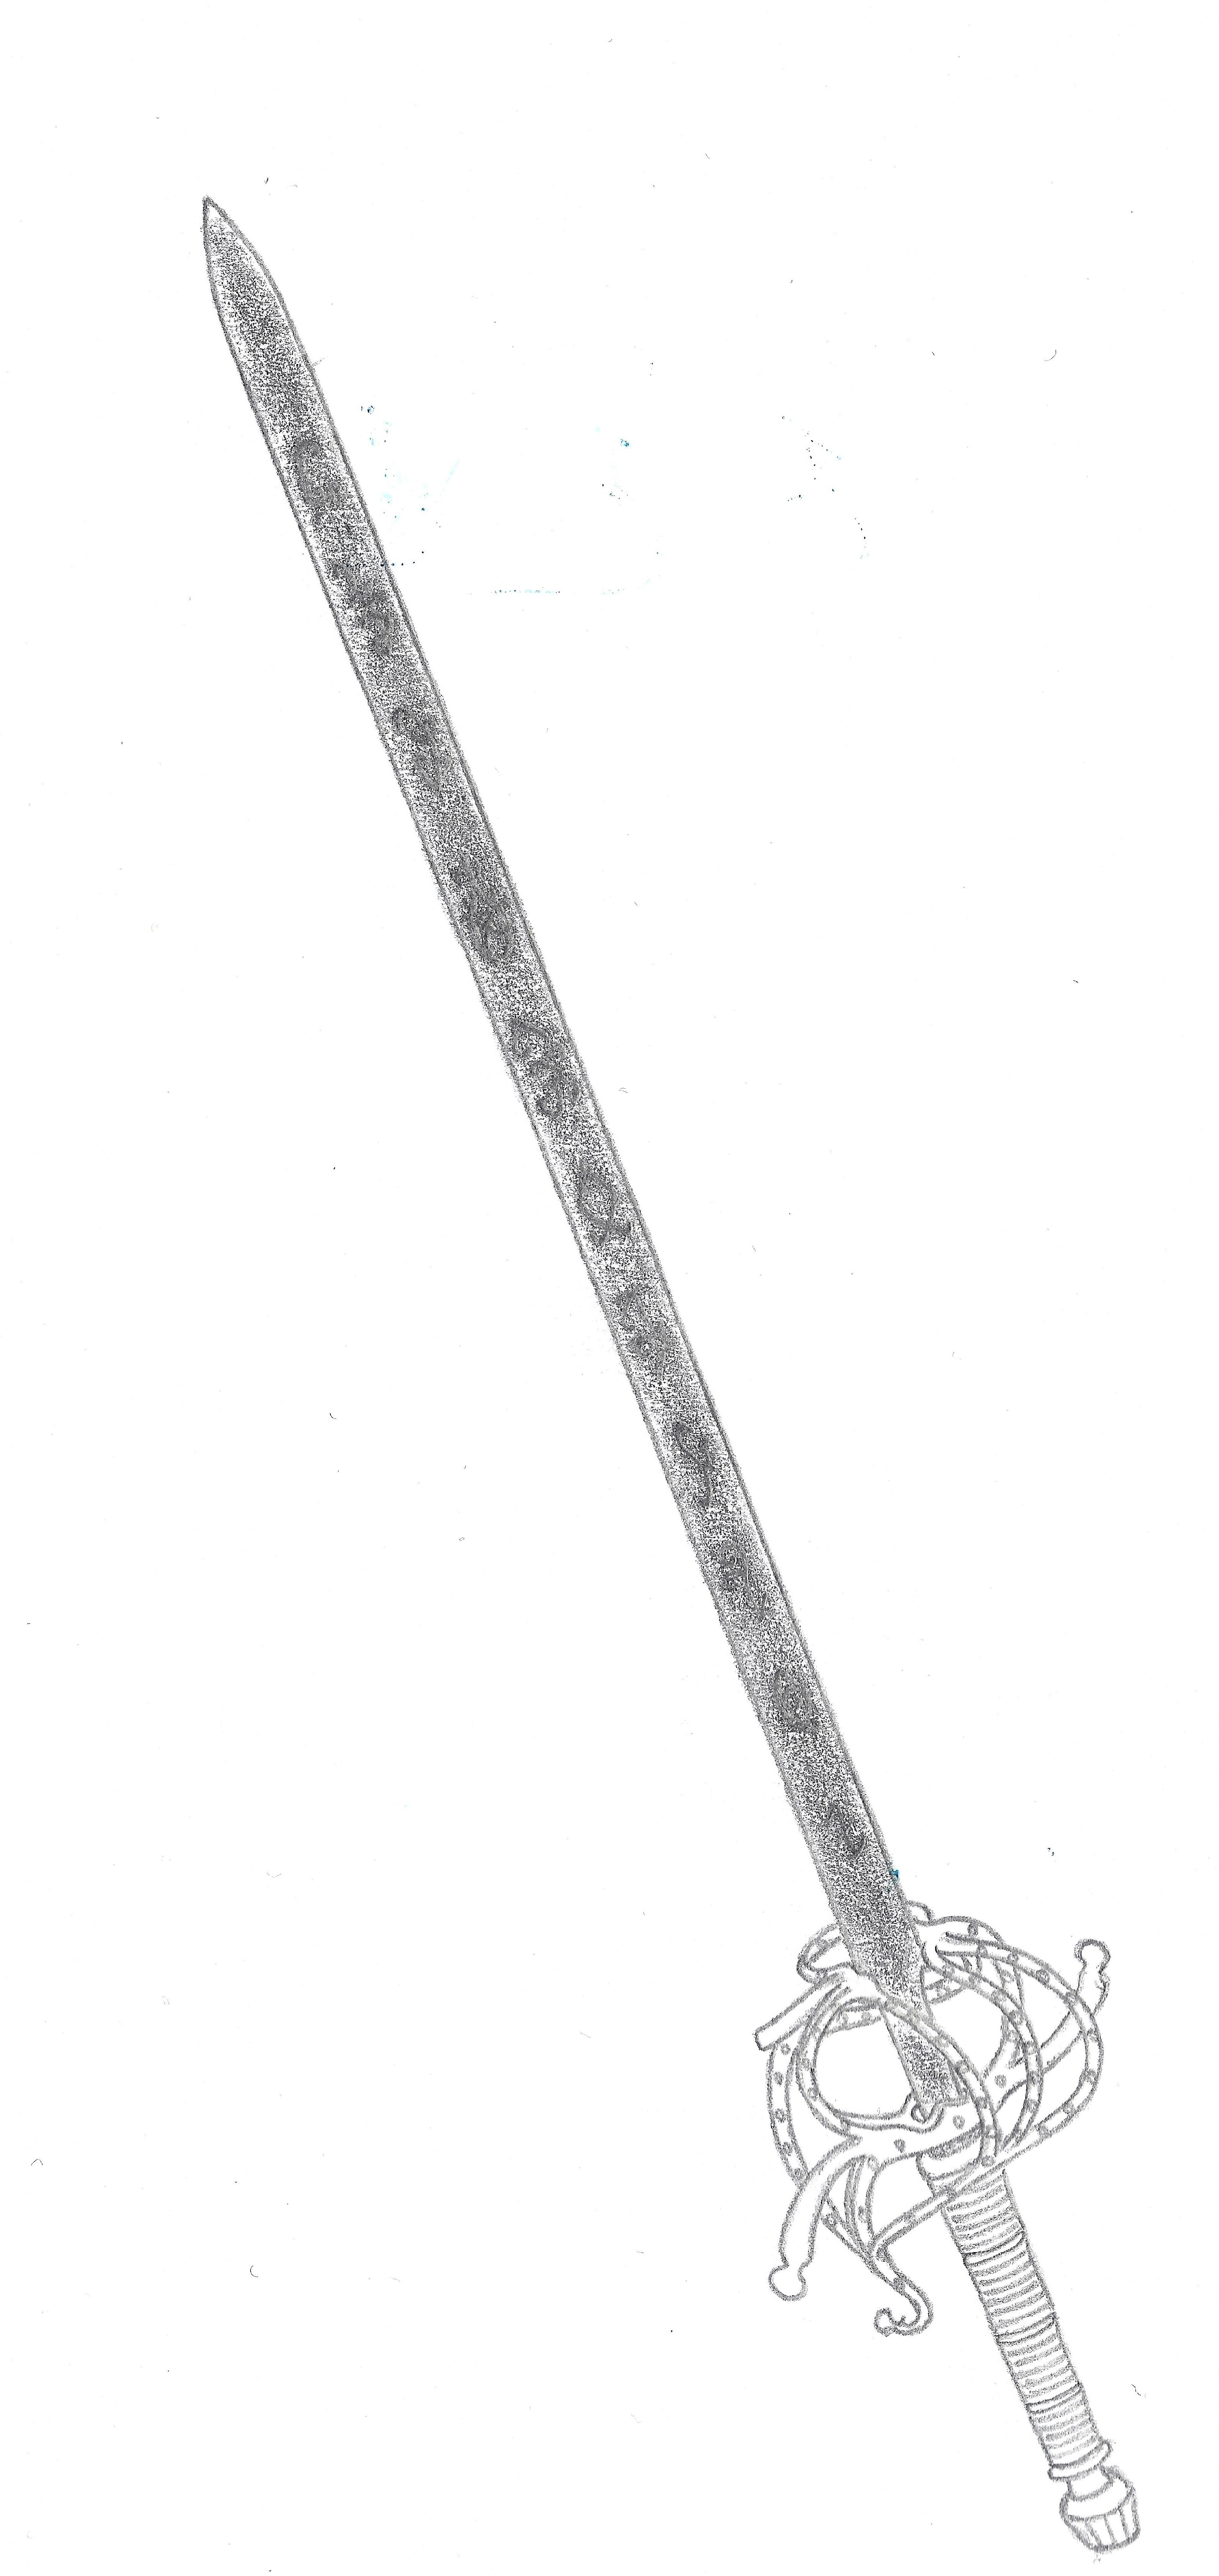
\includegraphics[width=\textwidth]{illustrations/firnen_endurium.jpg}
    \end{minipage}
    \begin{minipage}{0.3\linewidth}
    \centering
    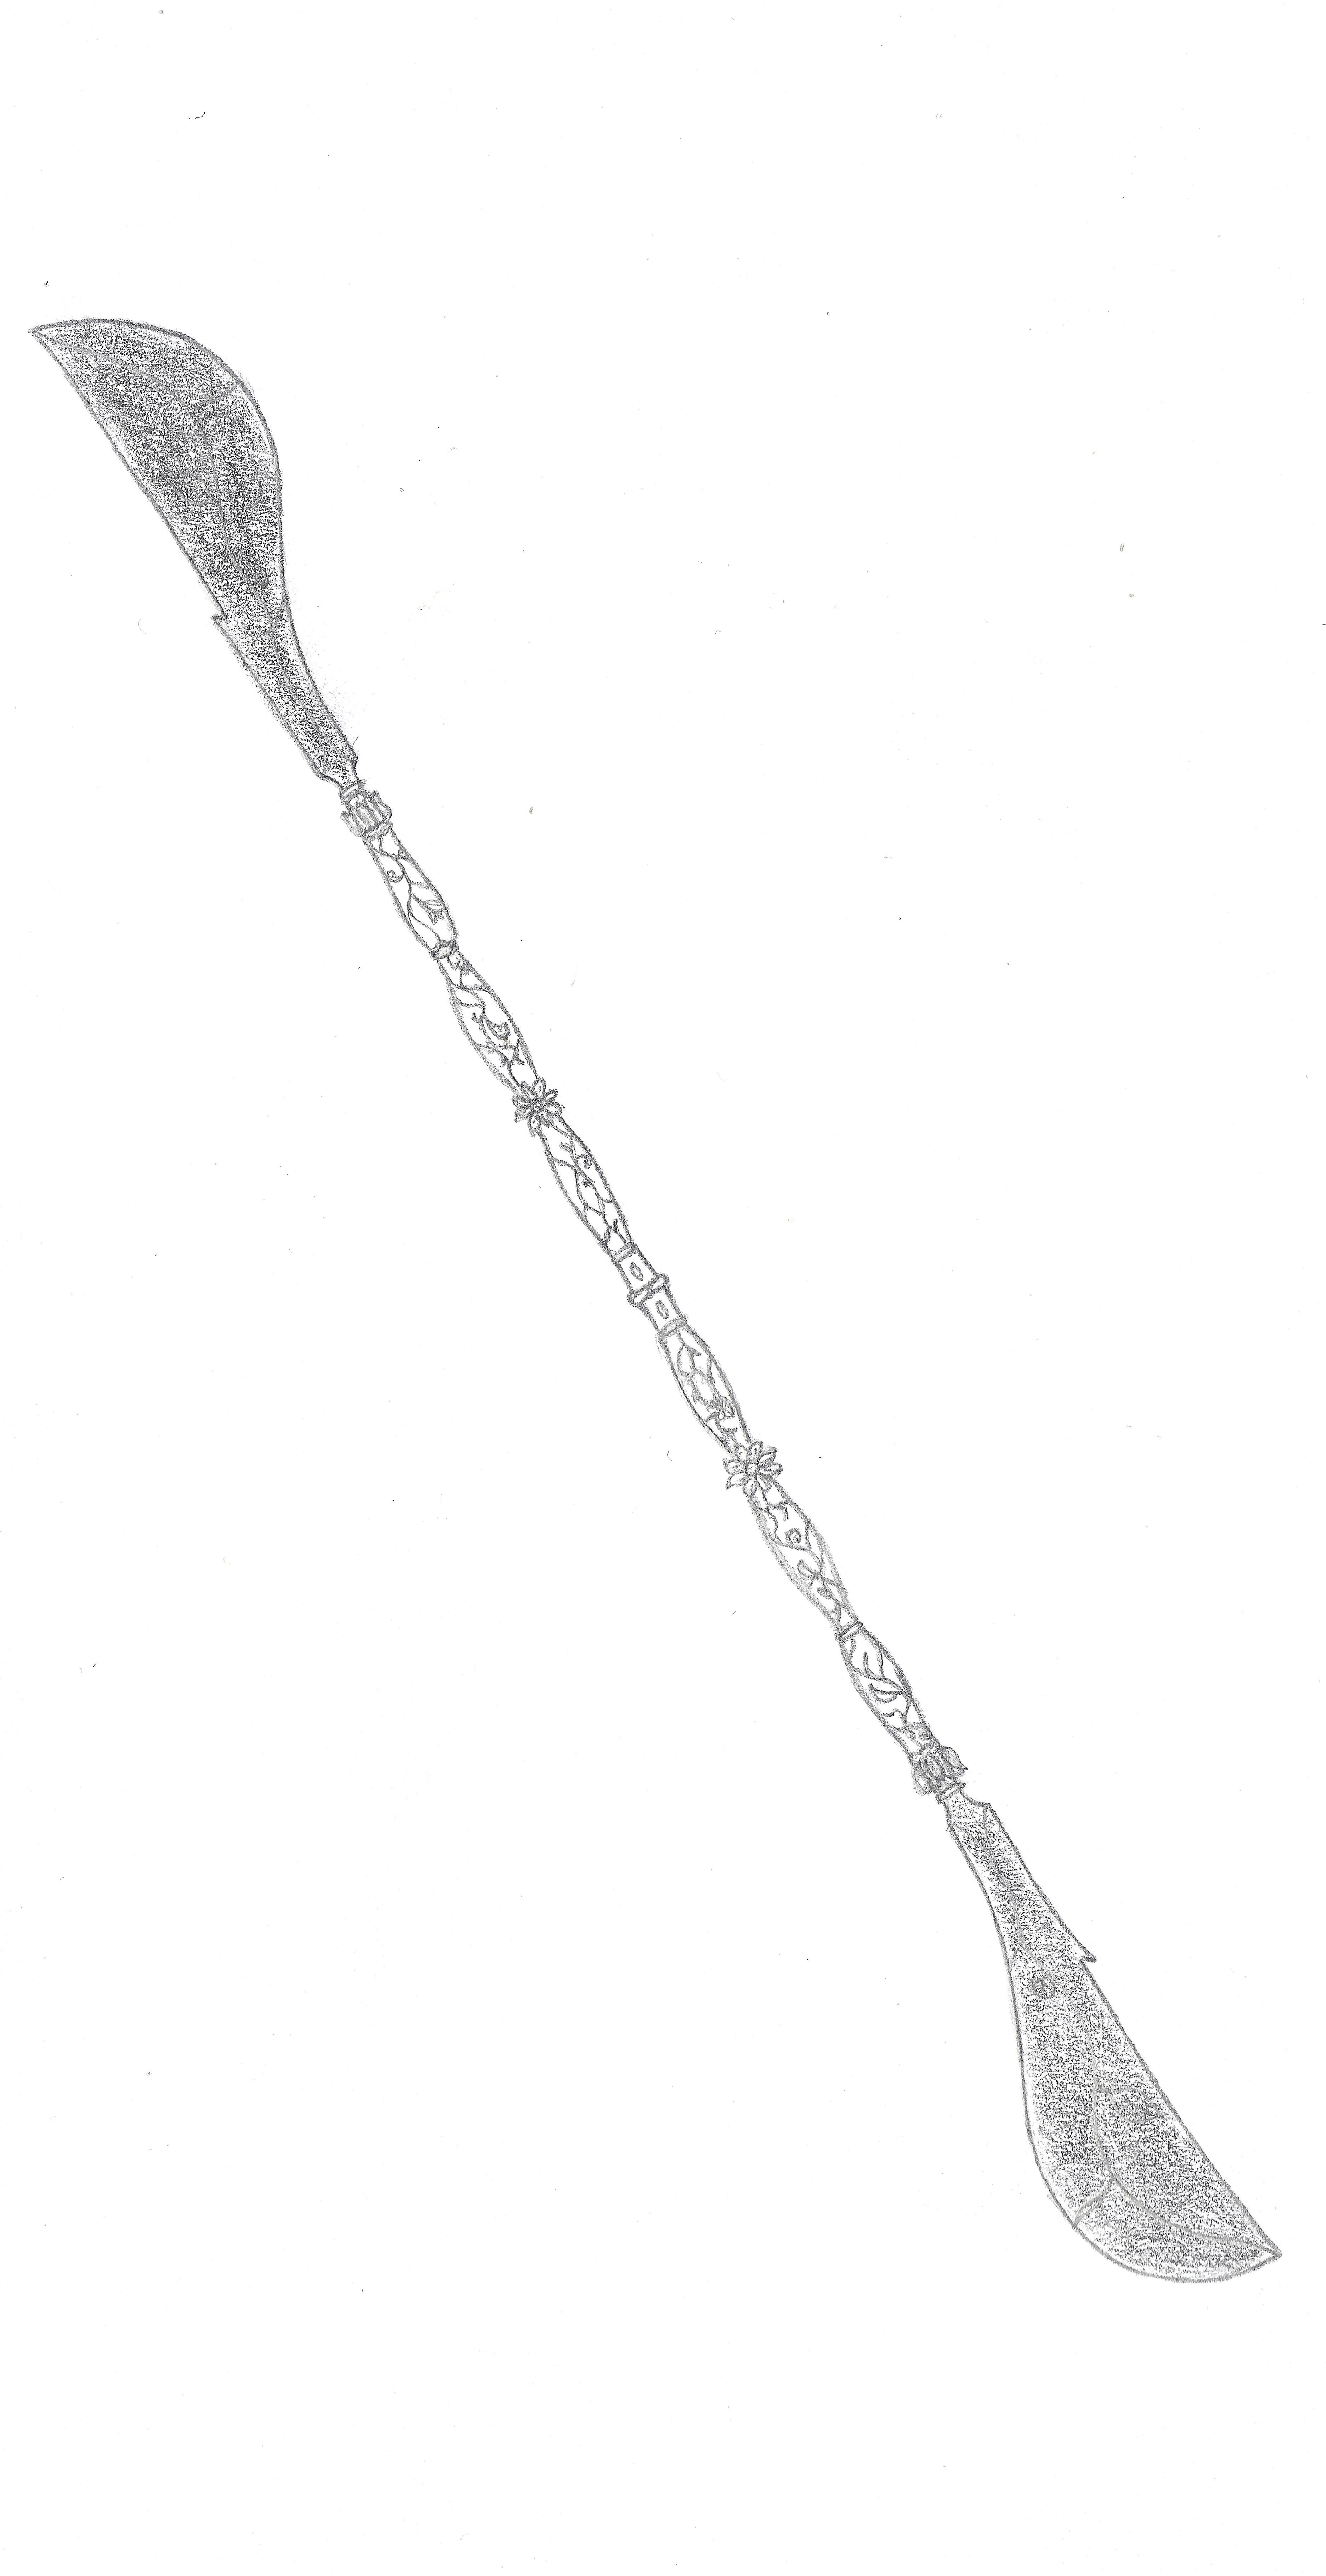
\includegraphics[width=\textwidth]{illustrations/toran_endurium.jpg}
    \end{minipage}
    \begin{minipage}{0.3\linewidth}
    \centering
    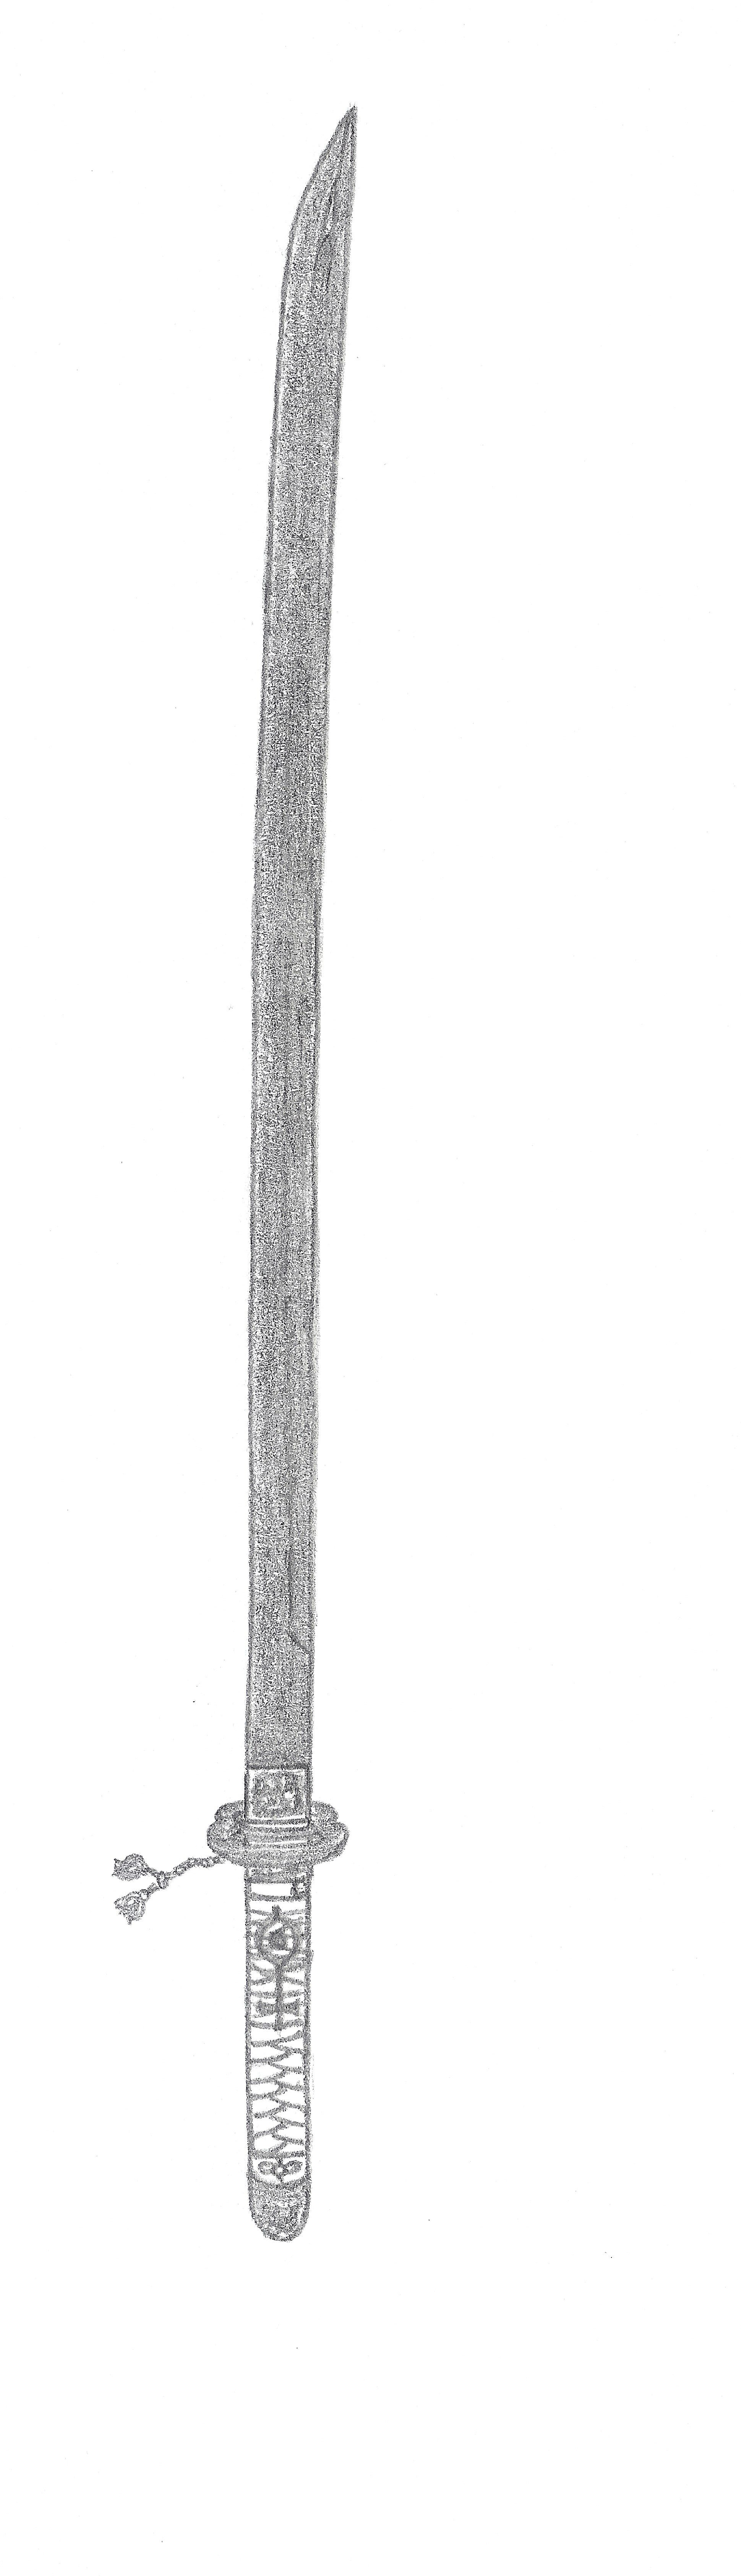
\includegraphics[width=0.6\textwidth]{illustrations/rezzanjin_endurium.jpg}
    \end{minipage}
\end{figure*}

\paragraph{Aussehen}
Der lange Magierdegen wurde aus feinstem Endurium gefertigt. Die Intarsien sind aus Mondsilber und bilden Schutz- und Bannglyphen in den magischen Runen des Arkanil. Das Heft ist von einem Kunstvollen Korb umflochten, der mit kleinen Quarzen besetzt ist.

\paragraph{Herstellung}
Das etwa ein Schritt lange Schwert ist ein Meisterwerk der Feinschmiedekunst, erschaffen von Sephira Eisenlieb, einer einfachen und doch begnadeten Geweihten des Ingerimm aus Angbar. 

\paragraph{Weihe}
Schwester Eisenlieb weihte das Werk permanent dem Ingerimm im Tempel des Ingerimm zu Angbar.


\section{Die Zweililie des Toran Ostik: Zahrabel, Blüte der Herrin}

\paragraph{Aussehen:}
Der Stab liegt schwerer in deiner Hand als dein alter, und ist aus dunklem Eichenholz gefertigt. Die Klingenblätter an beiden Enden glänzen schwarz und die Griffstange ist mit einem filigranen Geflecht aus geschnitzten Ranken und Blumen verziehrt. 

\paragraph{Herkunft:}
Der Stab der Waffe wurde dem Tsapriester Zadikar von Borbra von einem Elfen geschenkt, die Klingen wurden von einem Grangorer Meisterschmied gefertigt.

\paragraph{Weihe:}
Bruder Zadikar weihte die Zweililie permanent seiner Göttin um gegen die Pervertierung des Lebens stehen zu können.

\section{Das Schwert des Rezzanjin Al'Ahjan: Seyf, Schwert}

\paragraph{Aussehen:}
Das schwere Tuzakmesser ist etwas länger als üblich und aus tiefschwarzem Endurium gefertigt. Rote und Goldene Intarsien ziehen sich über die Klinge, wie Blut und geben der Waffe ein fließendes Aussehen. Der Griff ist mit rotem Leder umwickelt und mit goldenem Draht gesichert. Der Knauf wird von einem goldenen Löwenkopf geziert. 

\paragraph{Herkunft:}
Der Erschaffer dieses Meisterwerks ist der maraskanische Exilant Mulziber von Tuzak, der Schüler und Erbe des legendären Meisterschmiedes Grijomacon, der einst das Kaiserschwert Silpion erschuf.

\paragraph{Weihe:}
Die Erhabene Ayla von Schattengrund weihte die Waffe in einer Zeremonie feierlich permanent der leuengleichen Göttin Rondra.

\section{Der Bogen des Ragnos vom Svelltal: Cúnamorn ar Cún'anga}

\paragraph{Aussehen:}
Der mächtige Kriegsbogen ist aus Steineiche gefertigt und größer als alle Bögen, die du bisher geführt hast. Der Griff und die Spitzen sind mit schwarzem Endurium beschlagen. Beide Hörner des Bogens gleichen den Hörnern des Drachen, den du in deinem jetzt schon legendären Kampf vertrieben hast.
Köcher mit hundert enduriumbestückten Pfeilen liegen bei, sowie sieben Pfeile mit roten Federn, die in eine Rehhaut eingeschlagen sind.

\paragraph{Herkunft:}
Der Bogen wurde vom Roten Pfeil, Tenobaal Totenamsel, aus einer Steineiche gefertigt und von einem elfischen Schmied aus Donnerbach mit Endurium verziehrt.

\paragraph{Weihe:}
Der Bogen wurde durch einen unbekannten Firunpriester permanent dem Grimmigen Wintervater geweiht.

\section{Das Schwert des Arngrimm von Ehrenstein: Wolfsklaue}

\paragraph{Aussehen:}
Das lange, schlanke Bastardschwert ist wie seine Geschwisterwaffen aus tiefschwarzem Endurium gefertigt. Die Klinge ist gerade und so perfekt glatt, dass sich trotz der Schwärze des Stahl dein Gesicht darin spiegelt, als du es ziehst. 
Das Heft ist aus Ebenholz gefertigt und mit Silber und Elfenbein beschlagen. Den Knauf ziehrt ein weißer Wolfskopf, dessen gelbe Augen glatt polierte Bernsteine sind.

\paragraph{Herkunft:}
Thorn Eisinger, der bekannteste Waffenschmied Gareths schmiedete das Schwert für den heldenhaften Spross des Hauses Eherenstein aus dem in Maraskan geraubten Endurium.

\paragraph{Weihe:}
Das Schwert wurde vom Raben persönlich in einer stillen Zeremonie dem Gott Boron permanent geweiht.

\begin{figure*}[b]
    \centering
    \begin{minipage}{0.3\linewidth}
    \centering
    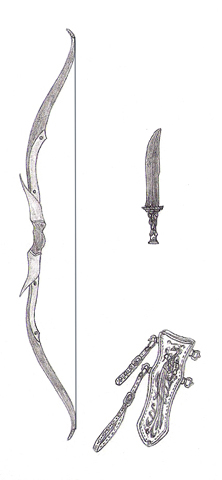
\includegraphics[width=\textwidth]{illustrations/ragnos_endurium.jpg}
    \end{minipage}
    \begin{minipage}{0.3\linewidth}
    \centering
    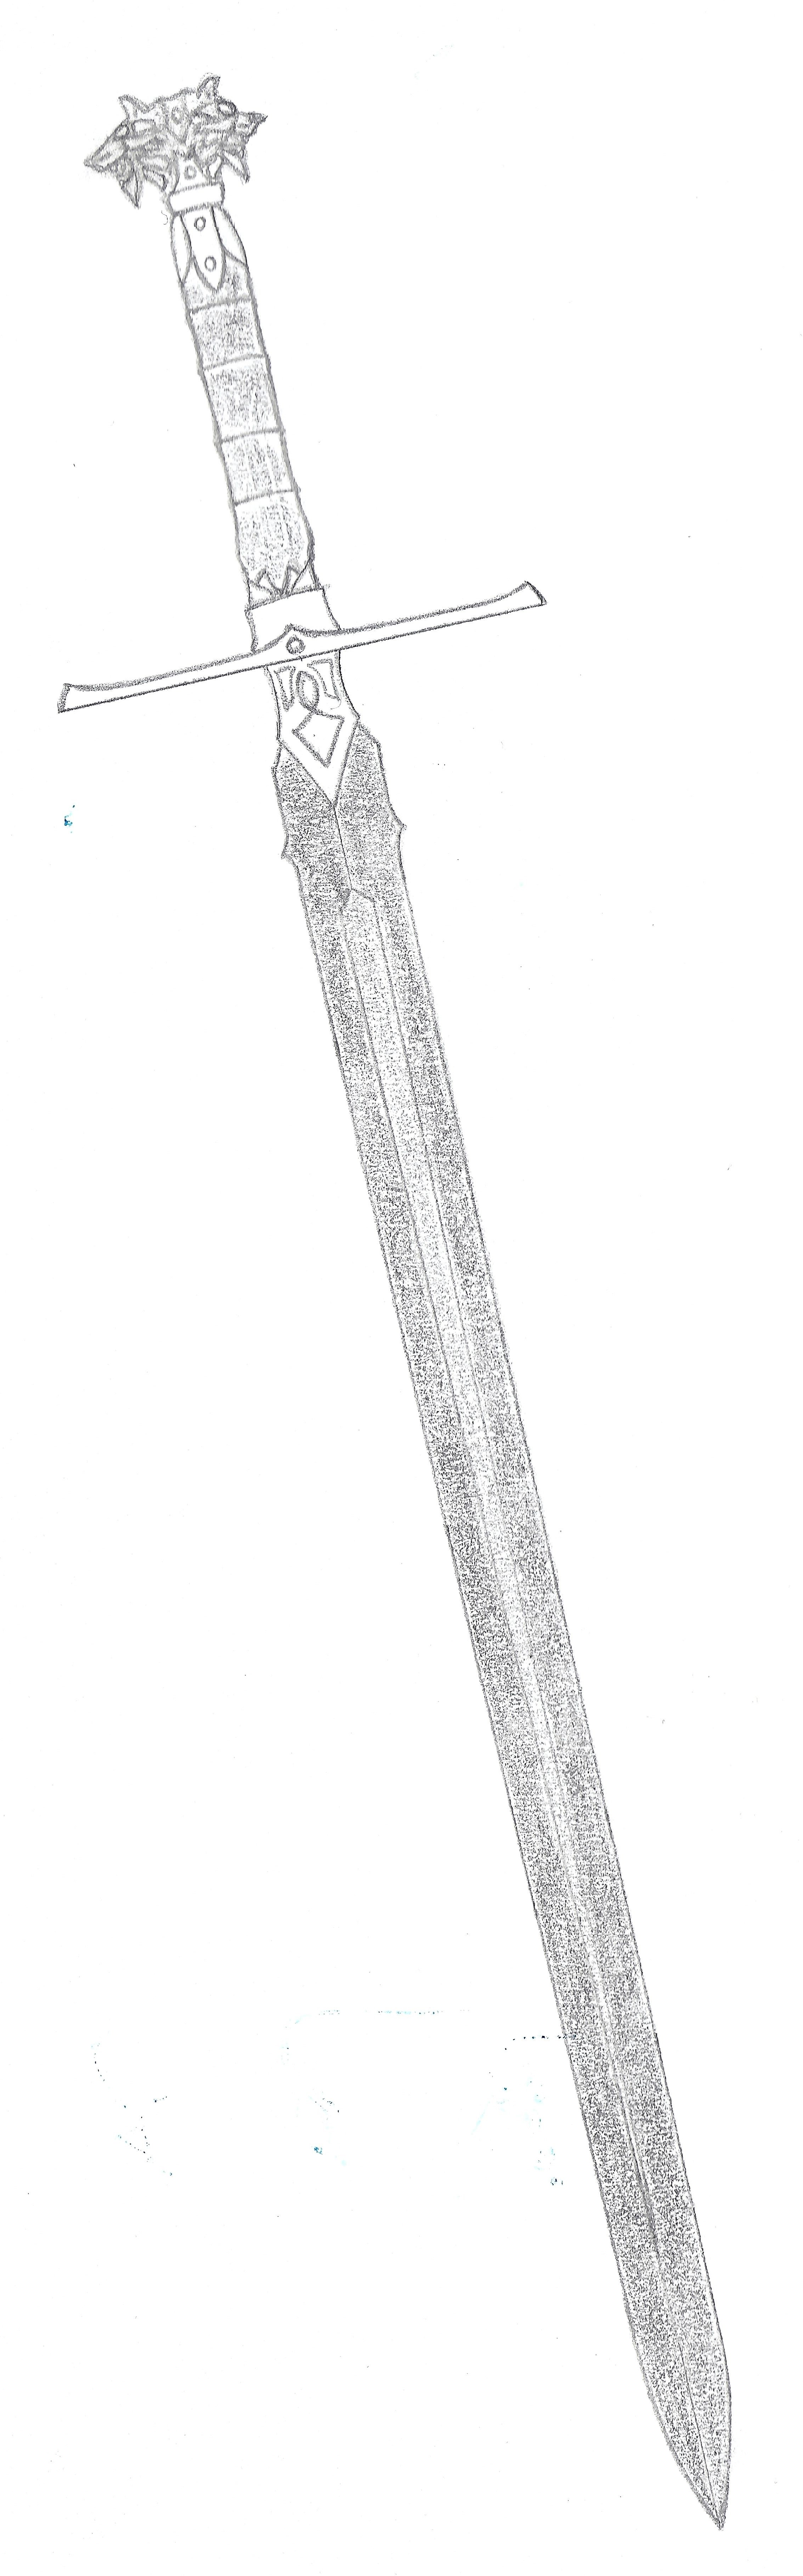
\includegraphics[width=0.6\textwidth]{illustrations/irian_endurium.jpg}
    \end{minipage}
\end{figure*}

\newpage
\FloatBarrier


\includepdf[scale=0.9,pages=1]{handouts/part_4/rv_einladung_magierkonvent.pdf}

\includepdf[scale=0.9,pages=-]{handouts/part_4/rv_einladung_toran.pdf}
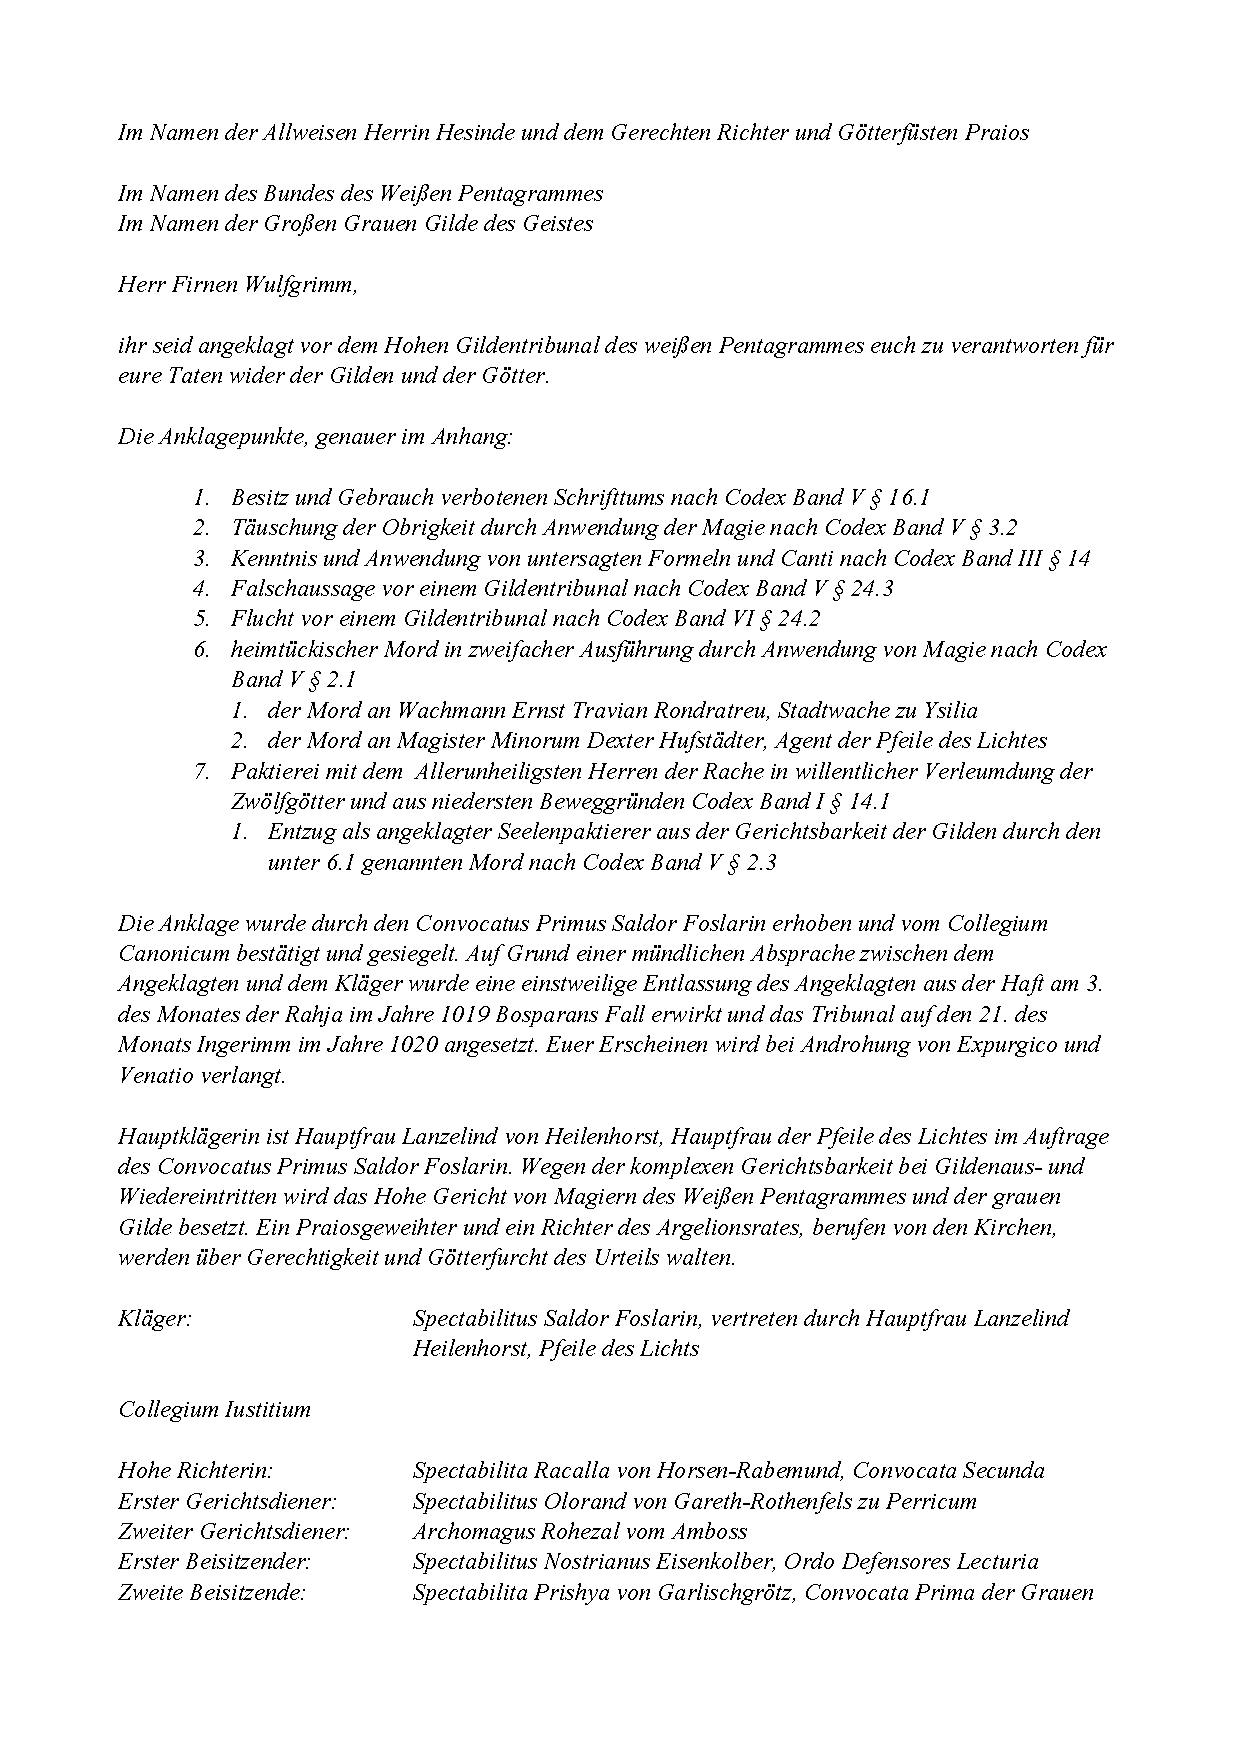
\includepdf[scale=0.9,pages=-]{handouts/part_4/rv_vorladung_firnen.pdf}
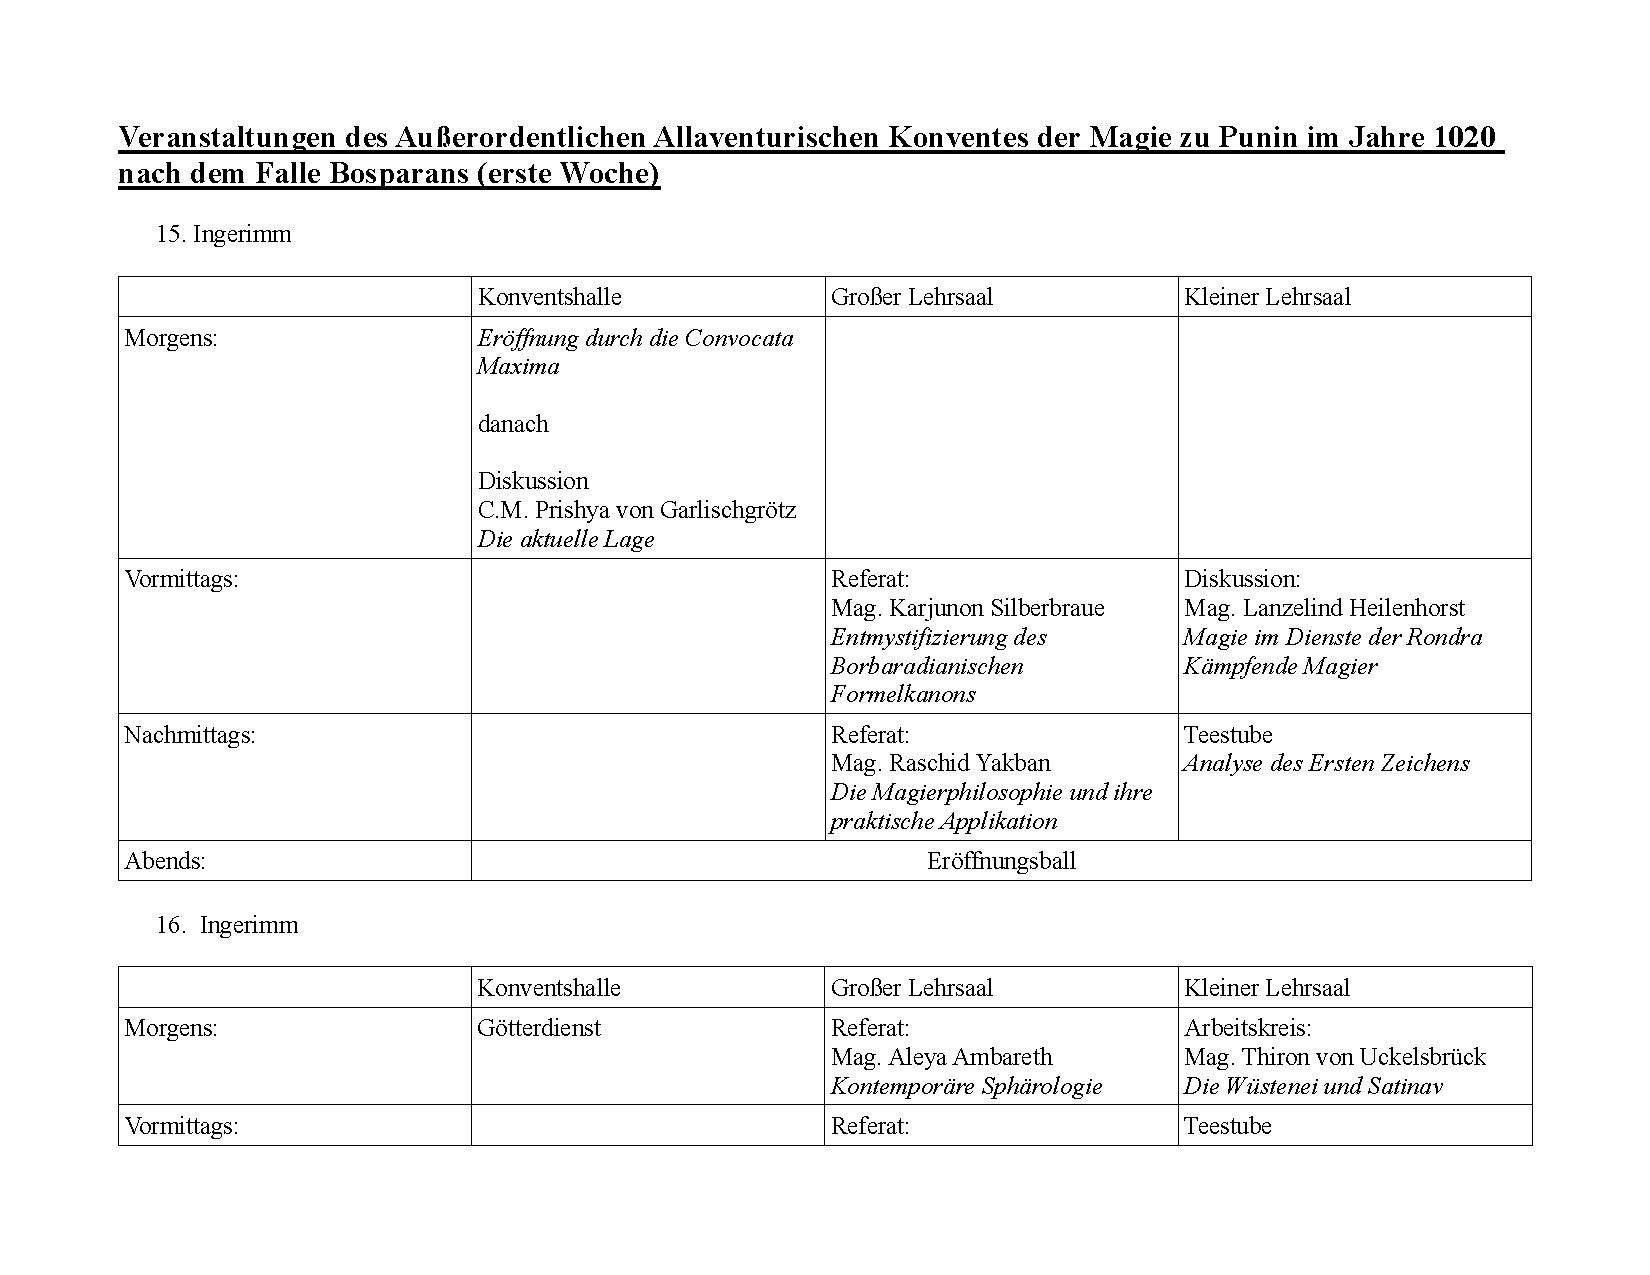
\includepdf[scale=1.0,pages=-,nup=1x2]{handouts/part_4/rv_tagesordnung.pdf}

\part{Die Zeichen}

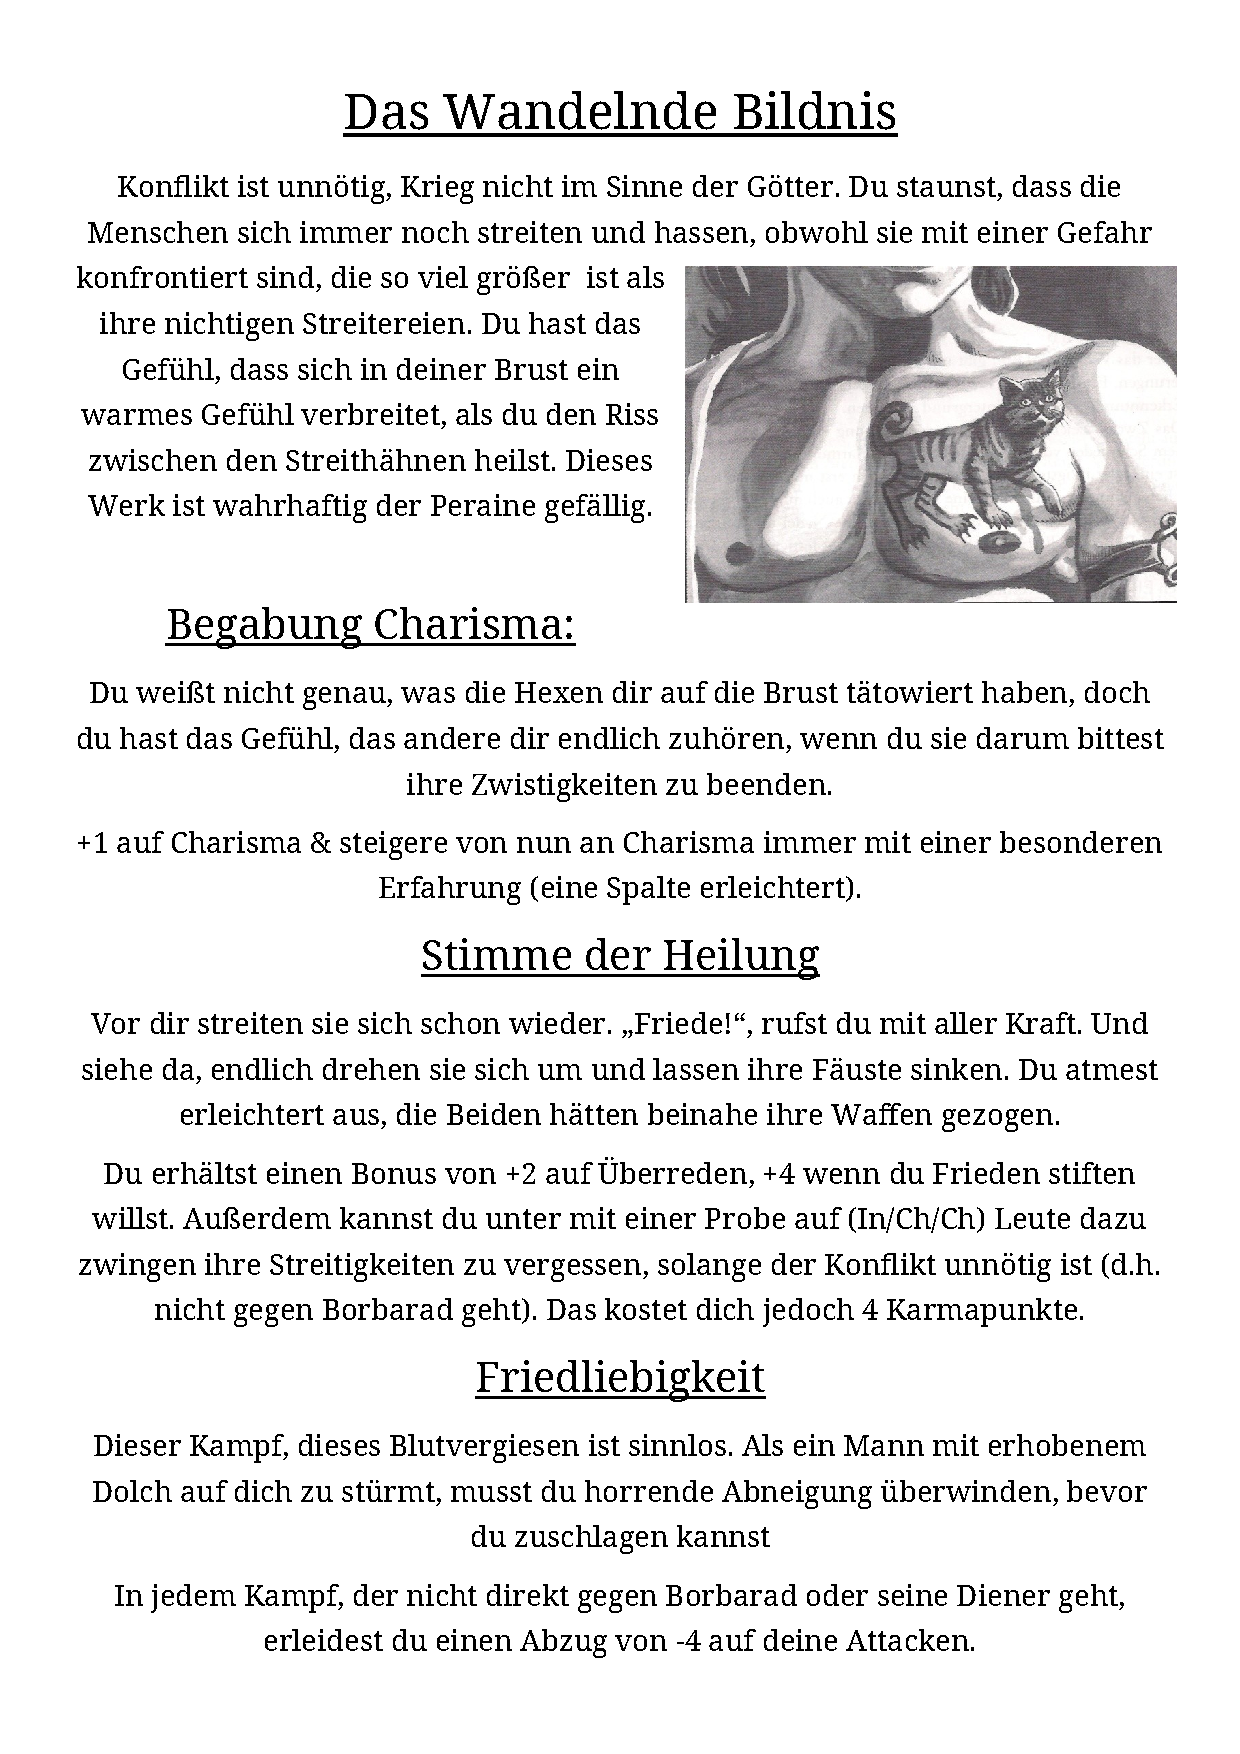
\includepdf[scale=0.9,pages=-]{handouts/zeichen/zweites_zeichen.pdf}
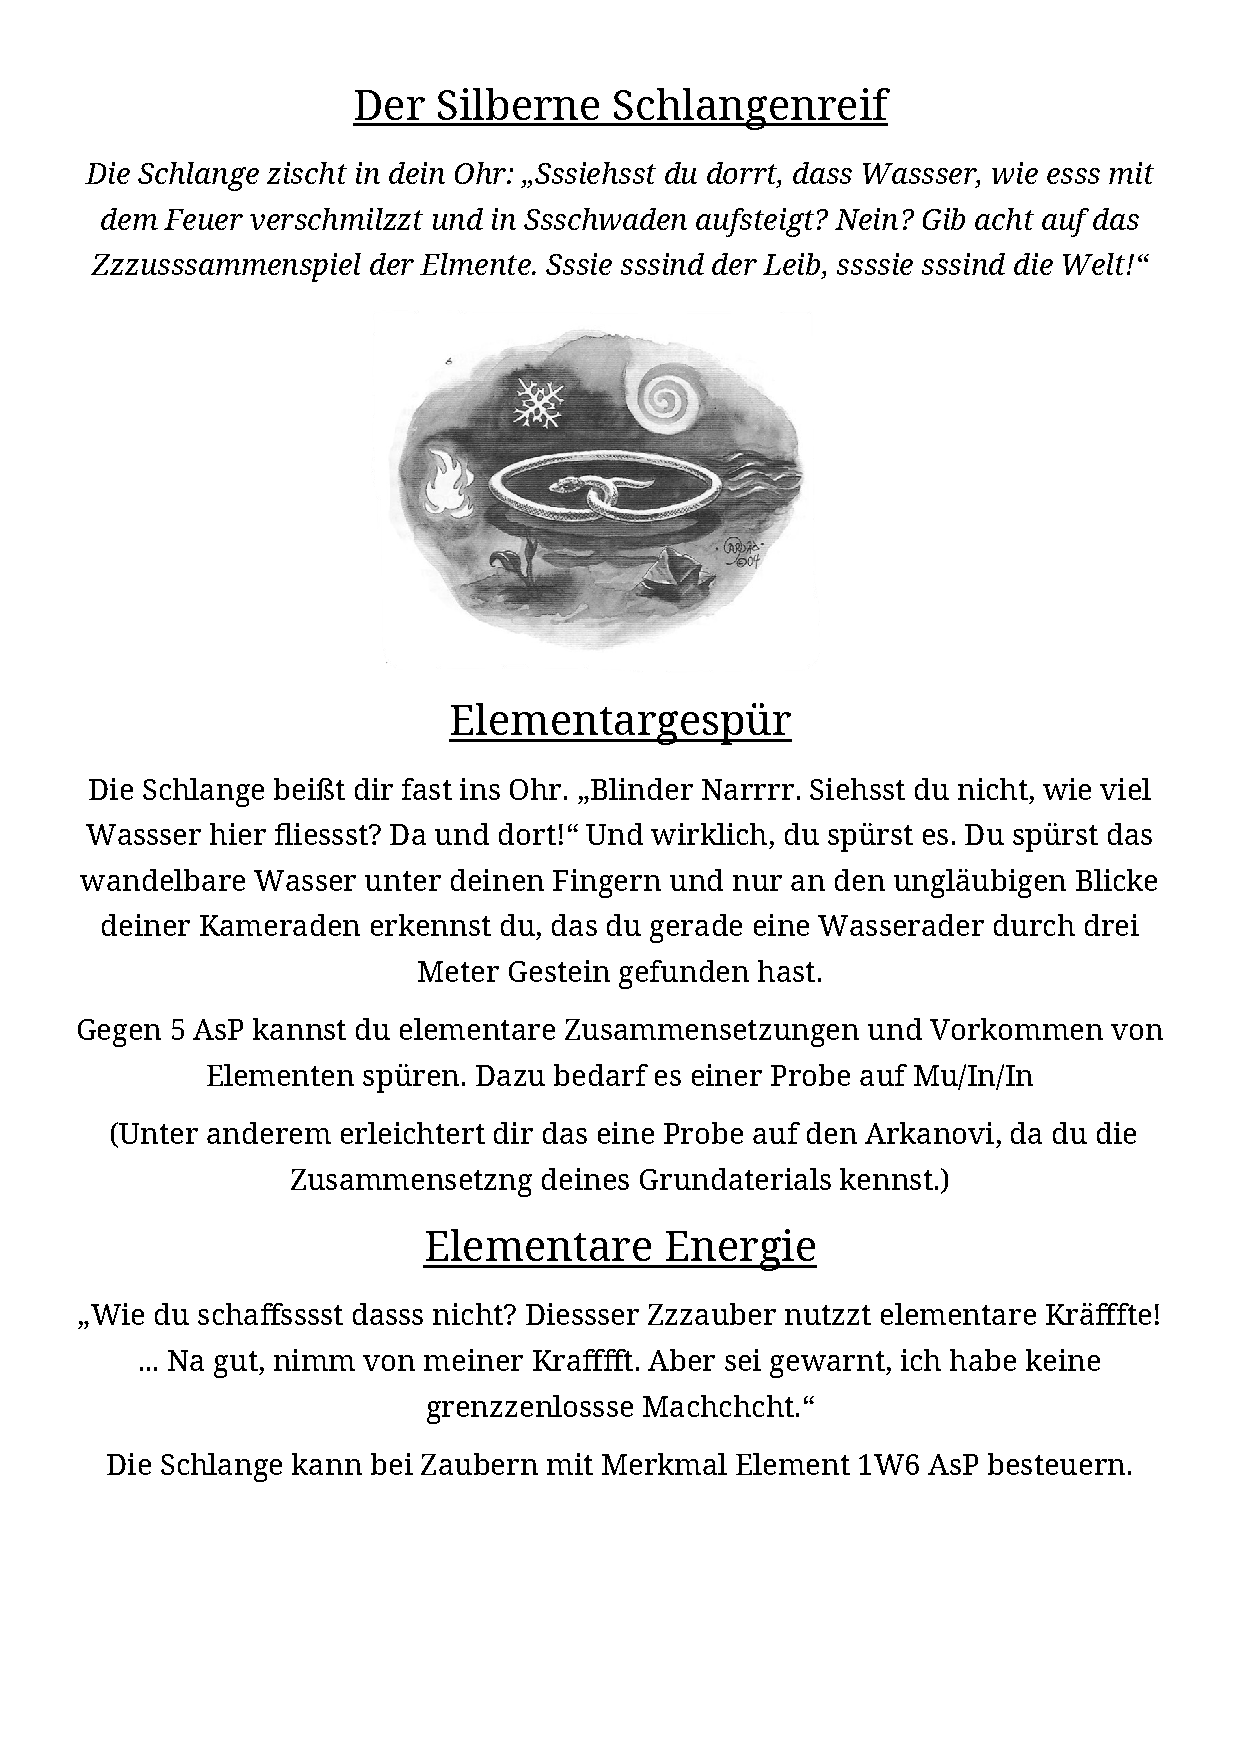
\includepdf[scale=0.9,pages=-]{handouts/zeichen/schlangenreif.pdf}
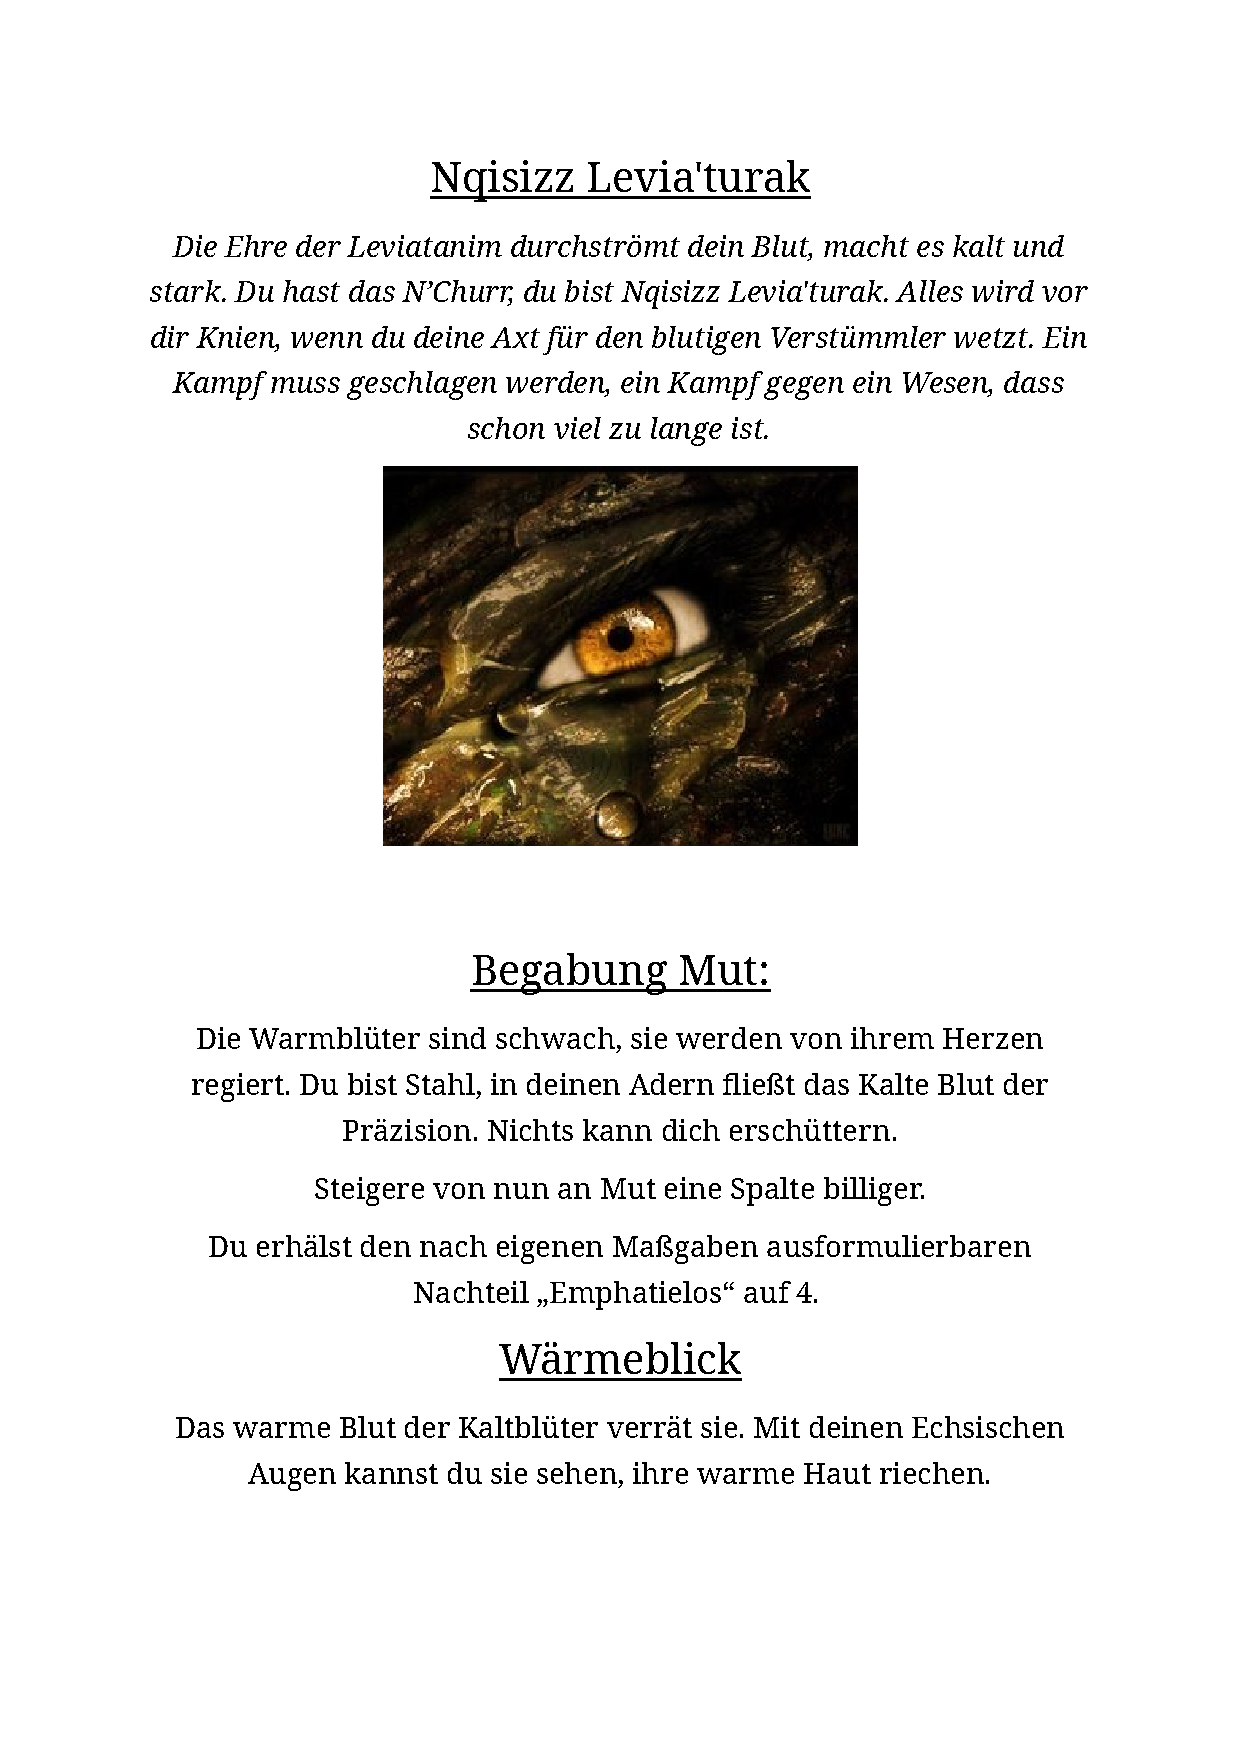
\includepdf[scale=0.9,pages=-]{handouts/zeichen/drittes_zeichen.pdf}

\part{Abschied}

\section{Verschmierter Brief, gefunden in den Unterlagen des verschollenen Waldemar Tiefhuser}

Lieber Waldemar,

Es ist wohl verständlich dass die Gezeichneten selbst keinen Bericht über die Geschehnisse an der Trollpforte ablegen konnten.
Und zugleich ist über die letzten Momente unserer Freunde sehr viel Tinte vergossen worden, so das ich kaum glaube, dass ich noch viel dazu beitragen könnte.

Aber die folgenden Informationen sind nur für deine Augen bestimmt, und unter den Lebenden befinden sich nur drei weitere, die um diese Geschehnisse wissen: Aria, Ayla, und ich. Tarlisin wird mir helfen meinen Weg zu beschreiten, aber selbst er kennt nicht die ganze Wahrheit.

Dies wird mein letzter Brief an dich sein. Nachdem er gesiegelt ist, wird der Hochmeister der Grauen Stäbe mich ins besetzte Maraskan schicken, wo ich sterben werde.
Wohin ich tatsächlich gehen werde, vermag ich dir nicht zu sagen, aber es wird kein Ort auf Deren sein.
Mir wurde eine Drachenschuppe zugespielt, ein wahrlich wunderschönes, und zugleich beängstigendes Artefakt.
Auf jener waren Worte eingeritzt, in einer Schrift, die ich nach all diesen Jahren kenne wie meine eigene: Ich habe eine Nachricht von Temyr erhalten, mit Informationen, wohin ich mich begeben soll.

Wir sehen uns wieder, eines Tages! Halte Ausschau nach einer Schuppen Menacors, denn alle, die an der Seite der Gezeichneten stritten, sind vorbestimmt die Schöpfung zu schützen.

Dein alter Freund,\\
Iliricon


\end{document}